\documentclass{book}
\usepackage[a4paper,top=2.5cm,bottom=2.5cm,left=2.5cm,right=2.5cm]{geometry}
\usepackage{makeidx}
\usepackage{natbib}
\usepackage{graphicx}
\usepackage{multicol}
\usepackage{float}
\usepackage{listings}
\usepackage{color}
\usepackage{ifthen}
\usepackage[table]{xcolor}
\usepackage{textcomp}
\usepackage{alltt}
\usepackage{ifpdf}
\ifpdf
\usepackage[pdftex,
            pagebackref=true,
            colorlinks=true,
            linkcolor=blue,
            unicode
           ]{hyperref}
\else
\usepackage[ps2pdf,
            pagebackref=true,
            colorlinks=true,
            linkcolor=blue,
            unicode
           ]{hyperref}
\usepackage{pspicture}
\fi
\usepackage[utf8]{inputenc}
\usepackage{mathptmx}
\usepackage[scaled=.90]{helvet}
\usepackage{courier}
\usepackage{sectsty}
\usepackage[titles]{tocloft}
\usepackage{doxygen}
\lstset{language=C++,inputencoding=utf8,basicstyle=\footnotesize,breaklines=true,breakatwhitespace=true,tabsize=4,numbers=left }
\makeindex
\setcounter{tocdepth}{3}
\renewcommand{\footrulewidth}{0.4pt}
\renewcommand{\familydefault}{\sfdefault}
\hfuzz=15pt
\setlength{\emergencystretch}{15pt}
\hbadness=750
\tolerance=750
\begin{document}
\hypersetup{pageanchor=false,citecolor=blue}
\begin{titlepage}
\vspace*{7cm}
\begin{center}
{\Large P\-B-\/\-S\-A\-M \\[1ex]\large V1 }\\
\vspace*{1cm}
{\large Generated by Doxygen 1.8.1}\\
\vspace*{0.5cm}
{\small Thu Aug 7 2014 13:09:03}\\
\end{center}
\end{titlepage}
\clearemptydoublepage
\pagenumbering{roman}
\tableofcontents
\clearemptydoublepage
\pagenumbering{arabic}
\hypersetup{pageanchor=true,citecolor=blue}
\chapter{Class Index}
\section{Class Hierarchy}
This inheritance list is sorted roughly, but not completely, alphabetically\-:\begin{DoxyCompactList}
\item \contentsline{section}{C\-B\-Dmulti}{\pageref{classCBDmulti}}{}
\item \contentsline{section}{C\-B\-Dnam}{\pageref{classCBDnam}}{}
\item \contentsline{section}{C\-Contact}{\pageref{classCContact}}{}
\item \contentsline{section}{C\-Expan}{\pageref{classCExpan}}{}
\begin{DoxyCompactList}
\item \contentsline{section}{C\-Local\-Expan}{\pageref{classCLocalExpan}}{}
\begin{DoxyCompactList}
\item \contentsline{section}{C\-L\-Expan}{\pageref{classCLExpan}}{}
\end{DoxyCompactList}
\item \contentsline{section}{C\-Mul\-Expan}{\pageref{classCMulExpan}}{}
\begin{DoxyCompactList}
\item \contentsline{section}{C\-M\-Expan}{\pageref{classCMExpan}}{}
\end{DoxyCompactList}
\item \contentsline{section}{C\-S\-H\-Expan}{\pageref{classCSHExpan}}{}
\begin{DoxyCompactList}
\item \contentsline{section}{C\-R\-Expan}{\pageref{classCRExpan}}{}
\begin{DoxyCompactList}
\item \contentsline{section}{C\-L\-Expan}{\pageref{classCLExpan}}{}
\item \contentsline{section}{C\-M\-Expan}{\pageref{classCMExpan}}{}
\end{DoxyCompactList}
\end{DoxyCompactList}
\end{DoxyCompactList}
\item \contentsline{section}{C\-Exp\-Center}{\pageref{classCExpCenter}}{}
\begin{DoxyCompactList}
\item \contentsline{section}{C\-Sol\-Exp\-Center}{\pageref{classCSolExpCenter}}{}
\end{DoxyCompactList}
\item \contentsline{section}{C\-Full\-Sphere\-I\-D}{\pageref{classCFullSphereID}}{}
\item \contentsline{section}{C\-Full\-Sphere\-I\-D\-Pair}{\pageref{classCFullSphereIDPair}}{}
\item \contentsline{section}{class\-Compare\-C\-Full\-Sphere\-I\-D}{\pageref{structclassCompareCFullSphereID}}{}
\item \contentsline{section}{class\-Compare\-C\-Full\-Sphere\-I\-D\-Pair}{\pageref{structclassCompareCFullSphereIDPair}}{}
\item \contentsline{section}{class\-Compare\-C\-Sphere\-I\-D\-Pair}{\pageref{structclassCompareCSphereIDPair}}{}
\item \contentsline{section}{C\-Mol\-Cell}{\pageref{classCMolCell}}{}
\item \contentsline{section}{C\-Mol\-Contact}{\pageref{classCMolContact}}{}
\item \contentsline{section}{C\-Mol\-Contact\-Rigid}{\pageref{classCMolContactRigid}}{}
\item \contentsline{section}{C\-Molecule}{\pageref{classCMolecule}}{}
\item \contentsline{section}{C\-Pnt}{\pageref{classCPnt}}{}
\item \contentsline{section}{C\-Quat}{\pageref{classCQuat}}{}
\item \contentsline{section}{C\-Range}{\pageref{classCRange}}{}
\item \contentsline{section}{C\-R\-Expan\-Constructor$<$ T $>$}{\pageref{classCRExpanConstructor}}{}
\item \contentsline{section}{C\-Rot\-Coeff}{\pageref{classCRotCoeff}}{}
\item \contentsline{section}{C\-Sphere\-I\-D}{\pageref{classCSphereID}}{}
\item \contentsline{section}{C\-Sphere\-I\-D\-Pair}{\pageref{classCSphereIDPair}}{}
\item \contentsline{section}{C\-Sp\-Pnt}{\pageref{classCSpPnt}}{}
\item \contentsline{section}{C\-System}{\pageref{classCSystem}}{}
\item \contentsline{section}{C\-Trans\-Coeff}{\pageref{classCTransCoeff}}{}
\item \contentsline{section}{C\-Transform}{\pageref{classCTransform}}{}
\begin{DoxyCompactList}
\item \contentsline{section}{C\-Lto\-L\-Transform\-Full}{\pageref{classCLtoLTransformFull}}{}
\item \contentsline{section}{C\-Lto\-M\-Transform\-Full}{\pageref{classCLtoMTransformFull}}{}
\item \contentsline{section}{C\-Mto\-L\-Transform\-Full}{\pageref{classCMtoLTransformFull}}{}
\item \contentsline{section}{C\-Mto\-M\-Transform\-Full}{\pageref{classCMtoMTransformFull}}{}
\end{DoxyCompactList}
\item \contentsline{section}{C\-Tri\-Expan}{\pageref{classCTriExpan}}{}
\begin{DoxyCompactList}
\item \contentsline{section}{C\-Grad\-Expan}{\pageref{classCGradExpan}}{}
\end{DoxyCompactList}
\item \contentsline{section}{C\-X\-Form\-Base}{\pageref{classCXFormBase}}{}
\begin{DoxyCompactList}
\item \contentsline{section}{C\-X\-Form\-A}{\pageref{classCXFormA}}{}
\begin{DoxyCompactList}
\item \contentsline{section}{C\-X\-Form\-A\-Intra}{\pageref{classCXFormAIntra}}{}
\end{DoxyCompactList}
\item \contentsline{section}{C\-X\-Form\-N}{\pageref{classCXFormN}}{}
\begin{DoxyCompactList}
\item \contentsline{section}{C\-X\-Form\-N\-Intra}{\pageref{classCXFormNIntra}}{}
\end{DoxyCompactList}
\end{DoxyCompactList}
\item \contentsline{section}{Grid\-Pnt}{\pageref{structGridPnt}}{}
\end{DoxyCompactList}

\chapter{Class Index}
\section{Class List}
Here are the classes, structs, unions and interfaces with brief descriptions\-:\begin{DoxyCompactList}
\item\contentsline{section}{\hyperlink{classCBDmulti}{C\-B\-Dmulti} }{\pageref{classCBDmulti}}{}
\item\contentsline{section}{\hyperlink{classCBDnam}{C\-B\-Dnam} \\*The \hyperlink{classCBDnam}{C\-B\-Dnam} class }{\pageref{classCBDnam}}{}
\item\contentsline{section}{\hyperlink{classCContact}{C\-Contact} \\*The \hyperlink{classCContact}{C\-Contact} class }{\pageref{classCContact}}{}
\item\contentsline{section}{\hyperlink{classCExpan}{C\-Expan} }{\pageref{classCExpan}}{}
\item\contentsline{section}{\hyperlink{classCExpCenter}{C\-Exp\-Center} \\*\hyperlink{classCExpCenter}{C\-Exp\-Center} class }{\pageref{classCExpCenter}}{}
\item\contentsline{section}{\hyperlink{classCFullSphereID}{C\-Full\-Sphere\-I\-D} \\*\hyperlink{classCFullSphereID}{C\-Full\-Sphere\-I\-D} class }{\pageref{classCFullSphereID}}{}
\item\contentsline{section}{\hyperlink{classCFullSphereIDPair}{C\-Full\-Sphere\-I\-D\-Pair} \\*\hyperlink{classCFullSphereIDPair}{C\-Full\-Sphere\-I\-D\-Pair} class }{\pageref{classCFullSphereIDPair}}{}
\item\contentsline{section}{\hyperlink{classCGradExpan}{C\-Grad\-Expan} }{\pageref{classCGradExpan}}{}
\item\contentsline{section}{\hyperlink{structclassCompareCFullSphereID}{class\-Compare\-C\-Full\-Sphere\-I\-D} \\*Class\-Compare\-C\-Full\-Sphere\-I\-D class }{\pageref{structclassCompareCFullSphereID}}{}
\item\contentsline{section}{\hyperlink{structclassCompareCFullSphereIDPair}{class\-Compare\-C\-Full\-Sphere\-I\-D\-Pair} \\*Class\-Compare\-C\-Full\-Sphere\-I\-D\-Pair class }{\pageref{structclassCompareCFullSphereIDPair}}{}
\item\contentsline{section}{\hyperlink{structclassCompareCSphereIDPair}{class\-Compare\-C\-Sphere\-I\-D\-Pair} \\*Class\-Compare\-C\-Sphere\-I\-D\-Pair class }{\pageref{structclassCompareCSphereIDPair}}{}
\item\contentsline{section}{\hyperlink{classCLExpan}{C\-L\-Expan} }{\pageref{classCLExpan}}{}
\item\contentsline{section}{\hyperlink{classCLocalExpan}{C\-Local\-Expan} }{\pageref{classCLocalExpan}}{}
\item\contentsline{section}{\hyperlink{classCLtoLTransformFull}{C\-Lto\-L\-Transform\-Full} }{\pageref{classCLtoLTransformFull}}{}
\item\contentsline{section}{\hyperlink{classCLtoMTransformFull}{C\-Lto\-M\-Transform\-Full} }{\pageref{classCLtoMTransformFull}}{}
\item\contentsline{section}{\hyperlink{classCMExpan}{C\-M\-Expan} }{\pageref{classCMExpan}}{}
\item\contentsline{section}{\hyperlink{classCMolCell}{C\-Mol\-Cell} \\*The \hyperlink{classCMolCell}{C\-Mol\-Cell} class }{\pageref{classCMolCell}}{}
\item\contentsline{section}{\hyperlink{classCMolContact}{C\-Mol\-Contact} \\*The \hyperlink{classCMolContact}{C\-Mol\-Contact} class }{\pageref{classCMolContact}}{}
\item\contentsline{section}{\hyperlink{classCMolContactRigid}{C\-Mol\-Contact\-Rigid} \\*The \hyperlink{classCMolContactRigid}{C\-Mol\-Contact\-Rigid} class }{\pageref{classCMolContactRigid}}{}
\item\contentsline{section}{\hyperlink{classCMolecule}{C\-Molecule} \\*The \hyperlink{classCMolecule}{C\-Molecule} class }{\pageref{classCMolecule}}{}
\item\contentsline{section}{\hyperlink{classCMtoLTransformFull}{C\-Mto\-L\-Transform\-Full} }{\pageref{classCMtoLTransformFull}}{}
\item\contentsline{section}{\hyperlink{classCMtoMTransformFull}{C\-Mto\-M\-Transform\-Full} }{\pageref{classCMtoMTransformFull}}{}
\item\contentsline{section}{\hyperlink{classCMulExpan}{C\-Mul\-Expan} }{\pageref{classCMulExpan}}{}
\item\contentsline{section}{\hyperlink{classCPnt}{C\-Pnt} \\*The \hyperlink{classCPnt}{C\-Pnt} class }{\pageref{classCPnt}}{}
\item\contentsline{section}{\hyperlink{classCQuat}{C\-Quat} \\*The quaternion class }{\pageref{classCQuat}}{}
\item\contentsline{section}{\hyperlink{classCRange}{C\-Range} }{\pageref{classCRange}}{}
\item\contentsline{section}{\hyperlink{classCRExpan}{C\-R\-Expan} }{\pageref{classCRExpan}}{}
\item\contentsline{section}{\hyperlink{classCRExpanConstructor}{C\-R\-Expan\-Constructor$<$ T $>$} }{\pageref{classCRExpanConstructor}}{}
\item\contentsline{section}{\hyperlink{classCRotCoeff}{C\-Rot\-Coeff} \\*The rotation coefficient class }{\pageref{classCRotCoeff}}{}
\item\contentsline{section}{\hyperlink{classCSHExpan}{C\-S\-H\-Expan} }{\pageref{classCSHExpan}}{}
\item\contentsline{section}{\hyperlink{classCSolExpCenter}{C\-Sol\-Exp\-Center} \\*\hyperlink{classCSolExpCenter}{C\-Sol\-Exp\-Center} class }{\pageref{classCSolExpCenter}}{}
\item\contentsline{section}{\hyperlink{classCSphereID}{C\-Sphere\-I\-D} \\*\hyperlink{classCSphereID}{C\-Sphere\-I\-D} class }{\pageref{classCSphereID}}{}
\item\contentsline{section}{\hyperlink{classCSphereIDPair}{C\-Sphere\-I\-D\-Pair} \\*\hyperlink{classCSphereIDPair}{C\-Sphere\-I\-D\-Pair} class }{\pageref{classCSphereIDPair}}{}
\item\contentsline{section}{\hyperlink{classCSpPnt}{C\-Sp\-Pnt} \\*The \hyperlink{classCSpPnt}{C\-Sp\-Pnt} class }{\pageref{classCSpPnt}}{}
\item\contentsline{section}{\hyperlink{classCSystem}{C\-System} \\*The \hyperlink{classCSystem}{C\-System} class }{\pageref{classCSystem}}{}
\item\contentsline{section}{\hyperlink{classCTransCoeff}{C\-Trans\-Coeff} \\*The Trans\-Coeff class }{\pageref{classCTransCoeff}}{}
\item\contentsline{section}{\hyperlink{classCTransform}{C\-Transform} }{\pageref{classCTransform}}{}
\item\contentsline{section}{\hyperlink{classCTriExpan}{C\-Tri\-Expan} \\*\hyperlink{classCTriExpan}{C\-Tri\-Expan} class }{\pageref{classCTriExpan}}{}
\item\contentsline{section}{\hyperlink{classCXFormA}{C\-X\-Form\-A} \\*The \hyperlink{classCXFormA}{C\-X\-Form\-A} class }{\pageref{classCXFormA}}{}
\item\contentsline{section}{\hyperlink{classCXFormAIntra}{C\-X\-Form\-A\-Intra} \\*The \hyperlink{classCXFormAIntra}{C\-X\-Form\-A\-Intra} class }{\pageref{classCXFormAIntra}}{}
\item\contentsline{section}{\hyperlink{classCXFormBase}{C\-X\-Form\-Base} \\*The \hyperlink{classCXFormBase}{C\-X\-Form\-Base} class }{\pageref{classCXFormBase}}{}
\item\contentsline{section}{\hyperlink{classCXFormN}{C\-X\-Form\-N} \\*The \hyperlink{classCXFormN}{C\-X\-Form\-N} class }{\pageref{classCXFormN}}{}
\item\contentsline{section}{\hyperlink{classCXFormNIntra}{C\-X\-Form\-N\-Intra} \\*The \hyperlink{classCXFormNIntra}{C\-X\-Form\-N\-Intra} class }{\pageref{classCXFormNIntra}}{}
\item\contentsline{section}{\hyperlink{structGridPnt}{Grid\-Pnt} \\*\hyperlink{structGridPnt}{Grid\-Pnt} structure }{\pageref{structGridPnt}}{}
\end{DoxyCompactList}

\chapter{File Index}
\section{File List}
Here is a list of all files with brief descriptions\-:\begin{DoxyCompactList}
\item\contentsline{section}{\hyperlink{BDmulti_8cpp}{B\-Dmulti.\-cpp} }{\pageref{BDmulti_8cpp}}{}
\item\contentsline{section}{\hyperlink{BDmulti_8h}{B\-Dmulti.\-h} }{\pageref{BDmulti_8h}}{}
\item\contentsline{section}{\hyperlink{BDmulti__main_8cpp}{B\-Dmulti\-\_\-main.\-cpp} }{\pageref{BDmulti__main_8cpp}}{}
\item\contentsline{section}{\hyperlink{BDnam_8cpp}{B\-Dnam.\-cpp} }{\pageref{BDnam_8cpp}}{}
\item\contentsline{section}{\hyperlink{BDnam_8h}{B\-Dnam.\-h} }{\pageref{BDnam_8h}}{}
\item\contentsline{section}{\hyperlink{BDnam__main_8cpp}{B\-Dnam\-\_\-main.\-cpp} }{\pageref{BDnam__main_8cpp}}{}
\item\contentsline{section}{\hyperlink{cell_8h}{cell.\-h} }{\pageref{cell_8h}}{}
\item\contentsline{section}{\hyperlink{contact_8cpp}{contact.\-cpp} }{\pageref{contact_8cpp}}{}
\item\contentsline{section}{\hyperlink{contact_8h}{contact.\-h} }{\pageref{contact_8h}}{}
\item\contentsline{section}{\hyperlink{contactRigid_8h}{contact\-Rigid.\-h} }{\pageref{contactRigid_8h}}{}
\item\contentsline{section}{\hyperlink{expansion_8cpp}{expansion.\-cpp} }{\pageref{expansion_8cpp}}{}
\item\contentsline{section}{\hyperlink{expansion_8h}{expansion.\-h} }{\pageref{expansion_8h}}{}
\item\contentsline{section}{\hyperlink{expcenter_8cpp}{expcenter.\-cpp} }{\pageref{expcenter_8cpp}}{}
\item\contentsline{section}{\hyperlink{expcenter_8h}{expcenter.\-h} }{\pageref{expcenter_8h}}{}
\item\contentsline{section}{\hyperlink{findContacts_8cpp}{find\-Contacts.\-cpp} }{\pageref{findContacts_8cpp}}{}
\item\contentsline{section}{\hyperlink{getmemory_8cpp}{getmemory.\-cpp} }{\pageref{getmemory_8cpp}}{}
\item\contentsline{section}{\hyperlink{getmemory_8h}{getmemory.\-h} }{\pageref{getmemory_8h}}{}
\item\contentsline{section}{\hyperlink{hash_8h}{hash.\-h} }{\pageref{hash_8h}}{}
\item\contentsline{section}{\hyperlink{lautil_8cpp}{lautil.\-cpp} }{\pageref{lautil_8cpp}}{}
\item\contentsline{section}{\hyperlink{lautil_8h}{lautil.\-h} }{\pageref{lautil_8h}}{}
\item\contentsline{section}{\hyperlink{makesphere_8cpp}{makesphere.\-cpp} }{\pageref{makesphere_8cpp}}{}
\item\contentsline{section}{\hyperlink{memory_8h}{memory.\-h} }{\pageref{memory_8h}}{}
\item\contentsline{section}{\hyperlink{moldynamics_8cpp}{moldynamics.\-cpp} }{\pageref{moldynamics_8cpp}}{}
\item\contentsline{section}{\hyperlink{molecule_8cpp}{molecule.\-cpp} }{\pageref{molecule_8cpp}}{}
\item\contentsline{section}{\hyperlink{molecule_8h}{molecule.\-h} }{\pageref{molecule_8h}}{}
\item\contentsline{section}{\hyperlink{readutil_8cpp}{readutil.\-cpp} }{\pageref{readutil_8cpp}}{}
\item\contentsline{section}{\hyperlink{readutil_8h}{readutil.\-h} }{\pageref{readutil_8h}}{}
\item\contentsline{section}{\hyperlink{rotcoeff_8cpp}{rotcoeff.\-cpp} }{\pageref{rotcoeff_8cpp}}{}
\item\contentsline{section}{\hyperlink{rotcoeff_8h}{rotcoeff.\-h} }{\pageref{rotcoeff_8h}}{}
\item\contentsline{section}{\hyperlink{selfp__makemat_8cpp}{selfp\-\_\-makemat.\-cpp} }{\pageref{selfp__makemat_8cpp}}{}
\item\contentsline{section}{\hyperlink{spheres_8cpp}{spheres.\-cpp} }{\pageref{spheres_8cpp}}{}
\item\contentsline{section}{\hyperlink{spheres_8h}{spheres.\-h} }{\pageref{spheres_8h}}{}
\item\contentsline{section}{\hyperlink{system_8cpp}{system.\-cpp} }{\pageref{system_8cpp}}{}
\item\contentsline{section}{\hyperlink{system_8h}{system.\-h} }{\pageref{system_8h}}{}
\item\contentsline{section}{\hyperlink{transcoeff_8cpp}{transcoeff.\-cpp} }{\pageref{transcoeff_8cpp}}{}
\item\contentsline{section}{\hyperlink{transcoeff_8h}{transcoeff.\-h} }{\pageref{transcoeff_8h}}{}
\item\contentsline{section}{\hyperlink{transform_8h}{transform.\-h} }{\pageref{transform_8h}}{}
\item\contentsline{section}{\hyperlink{triexpan_8cpp}{triexpan.\-cpp} }{\pageref{triexpan_8cpp}}{}
\item\contentsline{section}{\hyperlink{triexpan_8h}{triexpan.\-h} }{\pageref{triexpan_8h}}{}
\item\contentsline{section}{\hyperlink{util_8h}{util.\-h} }{\pageref{util_8h}}{}
\item\contentsline{section}{\hyperlink{xforms_8cpp}{xforms.\-cpp} }{\pageref{xforms_8cpp}}{}
\item\contentsline{section}{\hyperlink{xforms_8h}{xforms.\-h} }{\pageref{xforms_8h}}{}
\end{DoxyCompactList}

\chapter{Class Documentation}
\hypertarget{classCBDmulti}{\section{C\-B\-Dmulti Class Reference}
\label{classCBDmulti}\index{C\-B\-Dmulti@{C\-B\-Dmulti}}
}


{\ttfamily \#include $<$B\-Dmulti.\-h$>$}

\subsection*{Public Member Functions}
\begin{DoxyCompactItemize}
\item 
\hyperlink{classCBDmulti_a2091db088b9a6a1a6ec2b7c6c5d8996f}{C\-B\-Dmulti} (int Np1, int Np2, const vector$<$ char $\ast$ $>$ \&molfnames1, const vector$<$ char $\ast$ $>$ \&molfnames2, \hyperlink{util_8h_a5821460e95a0800cf9f24c38915cbbde}{R\-E\-A\-L} idiel)
\item 
\hyperlink{classCBDmulti_adab1c621face82806068b94f89d1417d}{$\sim$\-C\-B\-Dmulti} ()
\item 
void \hyperlink{classCBDmulti_a635ea038d73100f6945a69a7cfaf5f66}{reset\-Lattice} ()
\item 
void \hyperlink{classCBDmulti_ad3f1d4ade11ecb178d99125ba81fefe5}{restart\-Config} (char $\ast$configname)
\item 
double \hyperlink{classCBDmulti_a62bd0bcd8a4e060e63093d318f0b39c1}{run\-First\-Dock\-Time} (double maxtime, char $\ast$fname)
\item 
\hyperlink{classCMolecule}{C\-Molecule} $\ast$ \hyperlink{classCBDmulti_ae22be9dc35b7e0c97f778d917f12d56b}{get\-Mol} (int i)
\end{DoxyCompactItemize}
\subsection*{Static Public Member Functions}
\begin{DoxyCompactItemize}
\item 
static void \hyperlink{classCBDmulti_ab02b45910f422bc234e90ba4f5cfb7c3}{init\-Constants} (int n\-Mol\-Type)
\item 
static void \hyperlink{classCBDmulti_aa78e69e7897bef6e00108079323b3fb4}{add\-Mol\-Contact} (int mol1type, const vector$<$ \hyperlink{classCMolContact}{C\-Mol\-Contact} $>$ \&molcontactlist)
\item 
static \hyperlink{classCPnt}{C\-Pnt} \hyperlink{classCBDmulti_ae70695a83936614ba8b8ec9cd8f2728e}{get\-Rand\-Vec} (\hyperlink{util_8h_a5821460e95a0800cf9f24c38915cbbde}{R\-E\-A\-L} std)
\end{DoxyCompactItemize}
\subsection*{Public Attributes}
\begin{DoxyCompactItemize}
\item 
vector$<$ \hyperlink{classCMolecule}{C\-Molecule} $\ast$ $>$ \hyperlink{classCBDmulti_a1648f5007c6c0e3458e11e65f266bc9e}{m\-\_\-mols}
\item 
vector$<$ vector$<$ \hyperlink{classCPnt}{C\-Pnt} $>$ $>$ \hyperlink{classCBDmulti_a59241b29096bb88713aba753b0e0142c}{m\-\_\-\-S\-Pxes}
\item 
vector$<$ \hyperlink{classCMolCell}{C\-Mol\-Cell} $>$ \hyperlink{classCBDmulti_a477fcf39d8a1fe28e14dbc1580b4a250}{m\-\_\-molcells}
\end{DoxyCompactItemize}


\subsection{Constructor \& Destructor Documentation}
\hypertarget{classCBDmulti_a2091db088b9a6a1a6ec2b7c6c5d8996f}{\index{C\-B\-Dmulti@{C\-B\-Dmulti}!C\-B\-Dmulti@{C\-B\-Dmulti}}
\index{C\-B\-Dmulti@{C\-B\-Dmulti}!CBDmulti@{C\-B\-Dmulti}}
\subsubsection[{C\-B\-Dmulti}]{\setlength{\rightskip}{0pt plus 5cm}C\-B\-Dmulti\-::\-C\-B\-Dmulti (
\begin{DoxyParamCaption}
\item[{int}]{Np1, }
\item[{int}]{Np2, }
\item[{const vector$<$ char $\ast$ $>$ \&}]{molfnames1, }
\item[{const vector$<$ char $\ast$ $>$ \&}]{molfnames2, }
\item[{{\bf R\-E\-A\-L}}]{idiel}
\end{DoxyParamCaption}
)}}\label{classCBDmulti_a2091db088b9a6a1a6ec2b7c6c5d8996f}


Here is the call graph for this function\-:\nopagebreak
\begin{figure}[H]
\begin{center}
\leavevmode
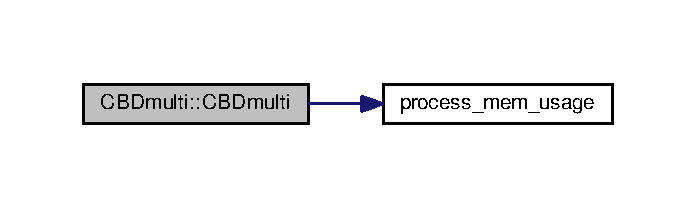
\includegraphics[width=334pt]{classCBDmulti_a2091db088b9a6a1a6ec2b7c6c5d8996f_cgraph}
\end{center}
\end{figure}


\hypertarget{classCBDmulti_adab1c621face82806068b94f89d1417d}{\index{C\-B\-Dmulti@{C\-B\-Dmulti}!$\sim$\-C\-B\-Dmulti@{$\sim$\-C\-B\-Dmulti}}
\index{$\sim$\-C\-B\-Dmulti@{$\sim$\-C\-B\-Dmulti}!CBDmulti@{C\-B\-Dmulti}}
\subsubsection[{$\sim$\-C\-B\-Dmulti}]{\setlength{\rightskip}{0pt plus 5cm}C\-B\-Dmulti\-::$\sim$\-C\-B\-Dmulti (
\begin{DoxyParamCaption}
{}
\end{DoxyParamCaption}
)\hspace{0.3cm}{\ttfamily [inline]}}}\label{classCBDmulti_adab1c621face82806068b94f89d1417d}


\subsection{Member Function Documentation}
\hypertarget{classCBDmulti_aa78e69e7897bef6e00108079323b3fb4}{\index{C\-B\-Dmulti@{C\-B\-Dmulti}!add\-Mol\-Contact@{add\-Mol\-Contact}}
\index{add\-Mol\-Contact@{add\-Mol\-Contact}!CBDmulti@{C\-B\-Dmulti}}
\subsubsection[{add\-Mol\-Contact}]{\setlength{\rightskip}{0pt plus 5cm}void C\-B\-Dmulti\-::add\-Mol\-Contact (
\begin{DoxyParamCaption}
\item[{int}]{mol1type, }
\item[{const vector$<$ {\bf C\-Mol\-Contact} $>$ \&}]{molcontactlist}
\end{DoxyParamCaption}
)\hspace{0.3cm}{\ttfamily [static]}}}\label{classCBDmulti_aa78e69e7897bef6e00108079323b3fb4}
\hypertarget{classCBDmulti_ae22be9dc35b7e0c97f778d917f12d56b}{\index{C\-B\-Dmulti@{C\-B\-Dmulti}!get\-Mol@{get\-Mol}}
\index{get\-Mol@{get\-Mol}!CBDmulti@{C\-B\-Dmulti}}
\subsubsection[{get\-Mol}]{\setlength{\rightskip}{0pt plus 5cm}{\bf C\-Molecule}$\ast$ C\-B\-Dmulti\-::get\-Mol (
\begin{DoxyParamCaption}
\item[{int}]{i}
\end{DoxyParamCaption}
)\hspace{0.3cm}{\ttfamily [inline]}}}\label{classCBDmulti_ae22be9dc35b7e0c97f778d917f12d56b}
\hypertarget{classCBDmulti_ae70695a83936614ba8b8ec9cd8f2728e}{\index{C\-B\-Dmulti@{C\-B\-Dmulti}!get\-Rand\-Vec@{get\-Rand\-Vec}}
\index{get\-Rand\-Vec@{get\-Rand\-Vec}!CBDmulti@{C\-B\-Dmulti}}
\subsubsection[{get\-Rand\-Vec}]{\setlength{\rightskip}{0pt plus 5cm}static {\bf C\-Pnt} C\-B\-Dmulti\-::get\-Rand\-Vec (
\begin{DoxyParamCaption}
\item[{{\bf R\-E\-A\-L}}]{std}
\end{DoxyParamCaption}
)\hspace{0.3cm}{\ttfamily [inline]}, {\ttfamily [static]}}}\label{classCBDmulti_ae70695a83936614ba8b8ec9cd8f2728e}


Here is the call graph for this function\-:\nopagebreak
\begin{figure}[H]
\begin{center}
\leavevmode
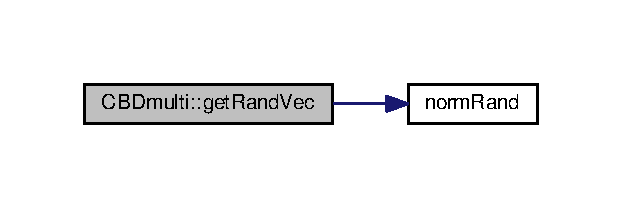
\includegraphics[width=298pt]{classCBDmulti_ae70695a83936614ba8b8ec9cd8f2728e_cgraph}
\end{center}
\end{figure}


\hypertarget{classCBDmulti_ab02b45910f422bc234e90ba4f5cfb7c3}{\index{C\-B\-Dmulti@{C\-B\-Dmulti}!init\-Constants@{init\-Constants}}
\index{init\-Constants@{init\-Constants}!CBDmulti@{C\-B\-Dmulti}}
\subsubsection[{init\-Constants}]{\setlength{\rightskip}{0pt plus 5cm}void C\-B\-Dmulti\-::init\-Constants (
\begin{DoxyParamCaption}
\item[{int}]{n\-Mol\-Type}
\end{DoxyParamCaption}
)\hspace{0.3cm}{\ttfamily [static]}}}\label{classCBDmulti_ab02b45910f422bc234e90ba4f5cfb7c3}
\hypertarget{classCBDmulti_a635ea038d73100f6945a69a7cfaf5f66}{\index{C\-B\-Dmulti@{C\-B\-Dmulti}!reset\-Lattice@{reset\-Lattice}}
\index{reset\-Lattice@{reset\-Lattice}!CBDmulti@{C\-B\-Dmulti}}
\subsubsection[{reset\-Lattice}]{\setlength{\rightskip}{0pt plus 5cm}void C\-B\-Dmulti\-::reset\-Lattice (
\begin{DoxyParamCaption}
{}
\end{DoxyParamCaption}
)}}\label{classCBDmulti_a635ea038d73100f6945a69a7cfaf5f66}


Here is the call graph for this function\-:\nopagebreak
\begin{figure}[H]
\begin{center}
\leavevmode
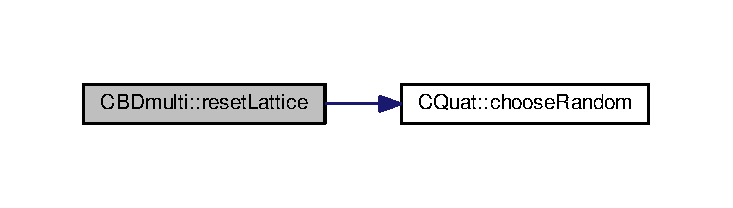
\includegraphics[width=350pt]{classCBDmulti_a635ea038d73100f6945a69a7cfaf5f66_cgraph}
\end{center}
\end{figure}


\hypertarget{classCBDmulti_ad3f1d4ade11ecb178d99125ba81fefe5}{\index{C\-B\-Dmulti@{C\-B\-Dmulti}!restart\-Config@{restart\-Config}}
\index{restart\-Config@{restart\-Config}!CBDmulti@{C\-B\-Dmulti}}
\subsubsection[{restart\-Config}]{\setlength{\rightskip}{0pt plus 5cm}void C\-B\-Dmulti\-::restart\-Config (
\begin{DoxyParamCaption}
\item[{char $\ast$}]{configname}
\end{DoxyParamCaption}
)}}\label{classCBDmulti_ad3f1d4ade11ecb178d99125ba81fefe5}
\hypertarget{classCBDmulti_a62bd0bcd8a4e060e63093d318f0b39c1}{\index{C\-B\-Dmulti@{C\-B\-Dmulti}!run\-First\-Dock\-Time@{run\-First\-Dock\-Time}}
\index{run\-First\-Dock\-Time@{run\-First\-Dock\-Time}!CBDmulti@{C\-B\-Dmulti}}
\subsubsection[{run\-First\-Dock\-Time}]{\setlength{\rightskip}{0pt plus 5cm}double C\-B\-Dmulti\-::run\-First\-Dock\-Time (
\begin{DoxyParamCaption}
\item[{double}]{maxtime, }
\item[{char $\ast$}]{fname}
\end{DoxyParamCaption}
)}}\label{classCBDmulti_a62bd0bcd8a4e060e63093d318f0b39c1}


Here is the call graph for this function\-:\nopagebreak
\begin{figure}[H]
\begin{center}
\leavevmode
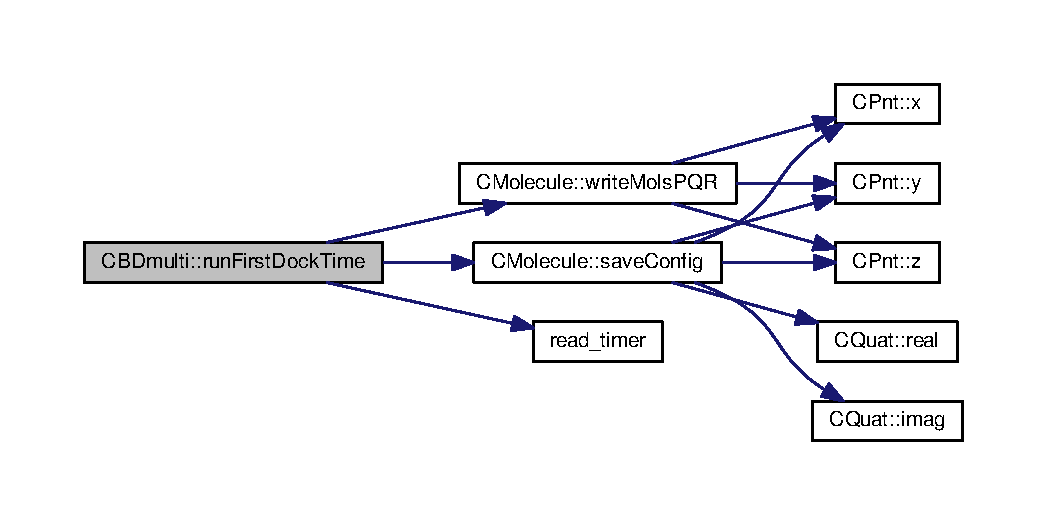
\includegraphics[width=350pt]{classCBDmulti_a62bd0bcd8a4e060e63093d318f0b39c1_cgraph}
\end{center}
\end{figure}




\subsection{Member Data Documentation}
\hypertarget{classCBDmulti_a477fcf39d8a1fe28e14dbc1580b4a250}{\index{C\-B\-Dmulti@{C\-B\-Dmulti}!m\-\_\-molcells@{m\-\_\-molcells}}
\index{m\-\_\-molcells@{m\-\_\-molcells}!CBDmulti@{C\-B\-Dmulti}}
\subsubsection[{m\-\_\-molcells}]{\setlength{\rightskip}{0pt plus 5cm}vector$<${\bf C\-Mol\-Cell}$>$ C\-B\-Dmulti\-::m\-\_\-molcells}}\label{classCBDmulti_a477fcf39d8a1fe28e14dbc1580b4a250}
\hypertarget{classCBDmulti_a1648f5007c6c0e3458e11e65f266bc9e}{\index{C\-B\-Dmulti@{C\-B\-Dmulti}!m\-\_\-mols@{m\-\_\-mols}}
\index{m\-\_\-mols@{m\-\_\-mols}!CBDmulti@{C\-B\-Dmulti}}
\subsubsection[{m\-\_\-mols}]{\setlength{\rightskip}{0pt plus 5cm}vector$<${\bf C\-Molecule}$\ast$$>$ C\-B\-Dmulti\-::m\-\_\-mols}}\label{classCBDmulti_a1648f5007c6c0e3458e11e65f266bc9e}
\hypertarget{classCBDmulti_a59241b29096bb88713aba753b0e0142c}{\index{C\-B\-Dmulti@{C\-B\-Dmulti}!m\-\_\-\-S\-Pxes@{m\-\_\-\-S\-Pxes}}
\index{m\-\_\-\-S\-Pxes@{m\-\_\-\-S\-Pxes}!CBDmulti@{C\-B\-Dmulti}}
\subsubsection[{m\-\_\-\-S\-Pxes}]{\setlength{\rightskip}{0pt plus 5cm}vector$<$vector$<${\bf C\-Pnt}$>$ $>$ C\-B\-Dmulti\-::m\-\_\-\-S\-Pxes}}\label{classCBDmulti_a59241b29096bb88713aba753b0e0142c}


The documentation for this class was generated from the following files\-:\begin{DoxyCompactItemize}
\item 
\hyperlink{BDmulti_8h}{B\-Dmulti.\-h}\item 
\hyperlink{BDmulti_8cpp}{B\-Dmulti.\-cpp}\end{DoxyCompactItemize}

\hypertarget{classCBDnam}{\section{C\-B\-Dnam Class Reference}
\label{classCBDnam}\index{C\-B\-Dnam@{C\-B\-Dnam}}
}


The \hyperlink{classCBDnam}{C\-B\-Dnam} class.  




{\ttfamily \#include $<$B\-Dnam.\-h$>$}

\subsection*{Public Types}
\begin{DoxyCompactItemize}
\item 
enum \hyperlink{classCBDnam_a9b511229c3d251ea1d4bae1c67d0ea8f}{S\-T\-A\-T\-U\-S} \{ \hyperlink{classCBDnam_a9b511229c3d251ea1d4bae1c67d0ea8fa9e12a628623c6235f9df2086d7b801ca}{E\-S\-C\-A\-P\-E\-D}, 
\hyperlink{classCBDnam_a9b511229c3d251ea1d4bae1c67d0ea8fabea72b0c444a7d389435b3b22be00b90}{D\-O\-C\-K\-E\-D}, 
\hyperlink{classCBDnam_a9b511229c3d251ea1d4bae1c67d0ea8fab5cac5babdaabba5b3c28b55b54bcfbc}{R\-U\-N\-N\-I\-N\-G}, 
\hyperlink{classCBDnam_a9b511229c3d251ea1d4bae1c67d0ea8fa09fbb1316278782c3117ea3c6192e696}{S\-T\-U\-C\-K}
 \}
\end{DoxyCompactItemize}
\subsection*{Public Member Functions}
\begin{DoxyCompactItemize}
\item 
\hyperlink{classCBDnam_a0032bfc247d677d5b6cd3937ed5f9fbb}{C\-B\-Dnam} (vector$<$ char $\ast$ $>$ molfnames1, vector$<$ char $\ast$ $>$ molfnames2, \hyperlink{util_8h_a5821460e95a0800cf9f24c38915cbbde}{R\-E\-A\-L} idiel)
\item 
\hyperlink{classCBDnam_a9b511229c3d251ea1d4bae1c67d0ea8f}{C\-B\-Dnam\-::\-S\-T\-A\-T\-U\-S} \hyperlink{classCBDnam_a07205701ed2267dc0457a4d621bb8aa8}{run} (int \&scount, char $\ast$fname)
\item 
\hyperlink{classCMolecule}{C\-Molecule} $\ast$ \hyperlink{classCBDnam_a715cfb64faa6369a733f9f6d0bd64350}{get\-Mol} (int i)
\end{DoxyCompactItemize}
\subsection*{Static Public Member Functions}
\begin{DoxyCompactItemize}
\item 
static void \hyperlink{classCBDnam_abee84e16de486d43f3bed18117c7031d}{init\-Constants} (int n\-Mol\-Type)
\item 
static void \hyperlink{classCBDnam_ab8b1d8c651f08545a9779617fbb3ba28}{add\-Mol\-Contact} (int mol1type, const vector$<$ \hyperlink{classCMolContact}{C\-Mol\-Contact} $>$ \&molcontactlist)
\item 
static \hyperlink{classCPnt}{C\-Pnt} \hyperlink{classCBDnam_a3f3175ac827dba969004309109e8e70c}{get\-Rand\-Vec} (\hyperlink{util_8h_a5821460e95a0800cf9f24c38915cbbde}{R\-E\-A\-L} std)
\end{DoxyCompactItemize}
\subsection*{Static Public Attributes}
\begin{DoxyCompactItemize}
\item 
static const char \hyperlink{classCBDnam_a0ca7d3cb1a694687bc249cb90bd549f0}{S\-T\-A\-T\-U\-S\-\_\-\-S\-T\-R\-I\-N\-G} \mbox{[}4\mbox{]}\mbox{[}10\mbox{]} = \{\char`\"{}E\-S\-C\-A\-P\-E\-D\char`\"{}, \char`\"{}\hyperlink{classCBDnam_a9b511229c3d251ea1d4bae1c67d0ea8fabea72b0c444a7d389435b3b22be00b90}{D\-O\-C\-K\-E\-D}\char`\"{}, \char`\"{}\hyperlink{classCBDnam_a9b511229c3d251ea1d4bae1c67d0ea8fab5cac5babdaabba5b3c28b55b54bcfbc}{R\-U\-N\-N\-I\-N\-G}\char`\"{}, \char`\"{}\hyperlink{classCBDnam_a9b511229c3d251ea1d4bae1c67d0ea8fa09fbb1316278782c3117ea3c6192e696}{S\-T\-U\-C\-K}\char`\"{}\}
\end{DoxyCompactItemize}


\subsection{Detailed Description}
The \hyperlink{classCBDnam}{C\-B\-Dnam} class. 

The class that contains information about a N\-A\-M run 

\subsection{Member Enumeration Documentation}
\hypertarget{classCBDnam_a9b511229c3d251ea1d4bae1c67d0ea8f}{\index{C\-B\-Dnam@{C\-B\-Dnam}!S\-T\-A\-T\-U\-S@{S\-T\-A\-T\-U\-S}}
\index{S\-T\-A\-T\-U\-S@{S\-T\-A\-T\-U\-S}!CBDnam@{C\-B\-Dnam}}
\subsubsection[{S\-T\-A\-T\-U\-S}]{\setlength{\rightskip}{0pt plus 5cm}enum {\bf C\-B\-Dnam\-::\-S\-T\-A\-T\-U\-S}}}\label{classCBDnam_a9b511229c3d251ea1d4bae1c67d0ea8f}
\begin{Desc}
\item[Enumerator\-: ]\par
\begin{description}
\index{E\-S\-C\-A\-P\-E\-D@{E\-S\-C\-A\-P\-E\-D}!C\-B\-Dnam@{C\-B\-Dnam}}\index{C\-B\-Dnam@{C\-B\-Dnam}!E\-S\-C\-A\-P\-E\-D@{E\-S\-C\-A\-P\-E\-D}}\item[{\em 
\hypertarget{classCBDnam_a9b511229c3d251ea1d4bae1c67d0ea8fa9e12a628623c6235f9df2086d7b801ca}{E\-S\-C\-A\-P\-E\-D}\label{classCBDnam_a9b511229c3d251ea1d4bae1c67d0ea8fa9e12a628623c6235f9df2086d7b801ca}
}]\index{D\-O\-C\-K\-E\-D@{D\-O\-C\-K\-E\-D}!C\-B\-Dnam@{C\-B\-Dnam}}\index{C\-B\-Dnam@{C\-B\-Dnam}!D\-O\-C\-K\-E\-D@{D\-O\-C\-K\-E\-D}}\item[{\em 
\hypertarget{classCBDnam_a9b511229c3d251ea1d4bae1c67d0ea8fabea72b0c444a7d389435b3b22be00b90}{D\-O\-C\-K\-E\-D}\label{classCBDnam_a9b511229c3d251ea1d4bae1c67d0ea8fabea72b0c444a7d389435b3b22be00b90}
}]\index{R\-U\-N\-N\-I\-N\-G@{R\-U\-N\-N\-I\-N\-G}!C\-B\-Dnam@{C\-B\-Dnam}}\index{C\-B\-Dnam@{C\-B\-Dnam}!R\-U\-N\-N\-I\-N\-G@{R\-U\-N\-N\-I\-N\-G}}\item[{\em 
\hypertarget{classCBDnam_a9b511229c3d251ea1d4bae1c67d0ea8fab5cac5babdaabba5b3c28b55b54bcfbc}{R\-U\-N\-N\-I\-N\-G}\label{classCBDnam_a9b511229c3d251ea1d4bae1c67d0ea8fab5cac5babdaabba5b3c28b55b54bcfbc}
}]\index{S\-T\-U\-C\-K@{S\-T\-U\-C\-K}!C\-B\-Dnam@{C\-B\-Dnam}}\index{C\-B\-Dnam@{C\-B\-Dnam}!S\-T\-U\-C\-K@{S\-T\-U\-C\-K}}\item[{\em 
\hypertarget{classCBDnam_a9b511229c3d251ea1d4bae1c67d0ea8fa09fbb1316278782c3117ea3c6192e696}{S\-T\-U\-C\-K}\label{classCBDnam_a9b511229c3d251ea1d4bae1c67d0ea8fa09fbb1316278782c3117ea3c6192e696}
}]\end{description}
\end{Desc}



\subsection{Constructor \& Destructor Documentation}
\hypertarget{classCBDnam_a0032bfc247d677d5b6cd3937ed5f9fbb}{\index{C\-B\-Dnam@{C\-B\-Dnam}!C\-B\-Dnam@{C\-B\-Dnam}}
\index{C\-B\-Dnam@{C\-B\-Dnam}!CBDnam@{C\-B\-Dnam}}
\subsubsection[{C\-B\-Dnam}]{\setlength{\rightskip}{0pt plus 5cm}C\-B\-Dnam\-::\-C\-B\-Dnam (
\begin{DoxyParamCaption}
\item[{vector$<$ char $\ast$ $>$}]{molfnames1, }
\item[{vector$<$ char $\ast$ $>$}]{molfnames2, }
\item[{{\bf R\-E\-A\-L}}]{idiel}
\end{DoxyParamCaption}
)}}\label{classCBDnam_a0032bfc247d677d5b6cd3937ed5f9fbb}
B\-Dnam constructor 

Here is the call graph for this function\-:\nopagebreak
\begin{figure}[H]
\begin{center}
\leavevmode
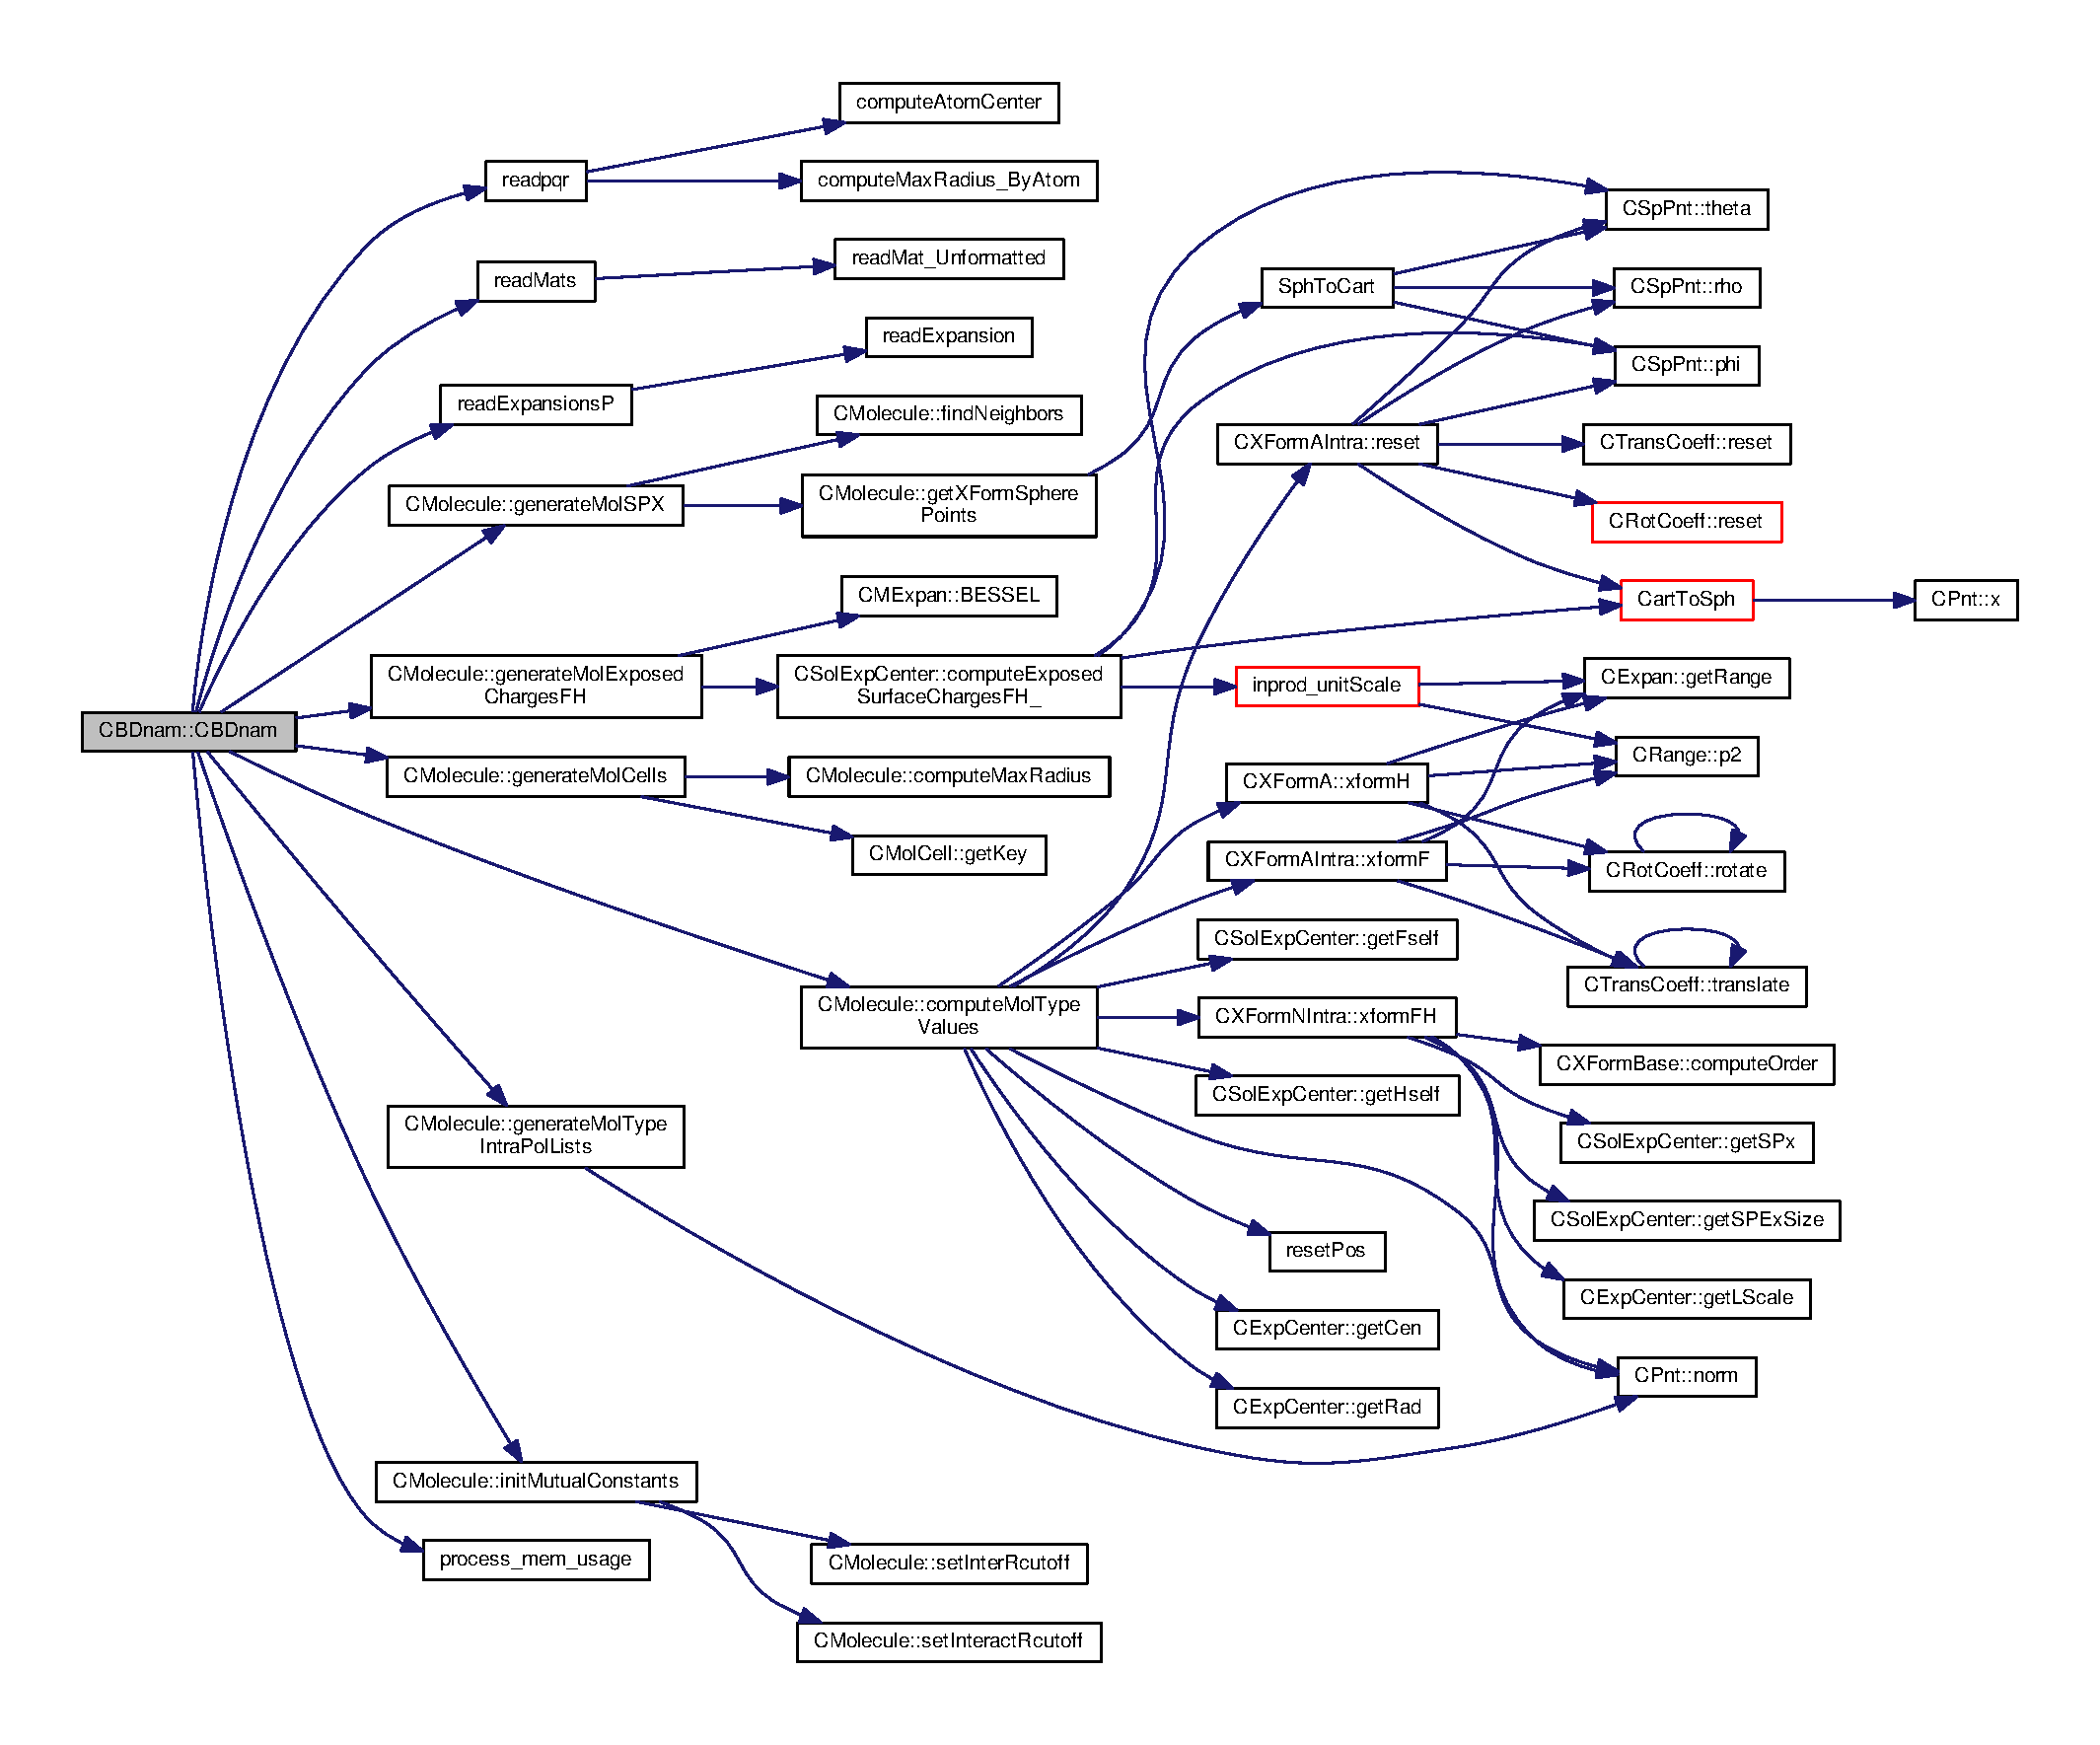
\includegraphics[width=350pt]{classCBDnam_a0032bfc247d677d5b6cd3937ed5f9fbb_cgraph}
\end{center}
\end{figure}




\subsection{Member Function Documentation}
\hypertarget{classCBDnam_ab8b1d8c651f08545a9779617fbb3ba28}{\index{C\-B\-Dnam@{C\-B\-Dnam}!add\-Mol\-Contact@{add\-Mol\-Contact}}
\index{add\-Mol\-Contact@{add\-Mol\-Contact}!CBDnam@{C\-B\-Dnam}}
\subsubsection[{add\-Mol\-Contact}]{\setlength{\rightskip}{0pt plus 5cm}void C\-B\-Dnam\-::add\-Mol\-Contact (
\begin{DoxyParamCaption}
\item[{int}]{mol1type, }
\item[{const vector$<$ {\bf C\-Mol\-Contact} $>$ \&}]{molcontactlist}
\end{DoxyParamCaption}
)\hspace{0.3cm}{\ttfamily [static]}}}\label{classCBDnam_ab8b1d8c651f08545a9779617fbb3ba28}
B\-Dnam add molecule to the contact list \hypertarget{classCBDnam_a715cfb64faa6369a733f9f6d0bd64350}{\index{C\-B\-Dnam@{C\-B\-Dnam}!get\-Mol@{get\-Mol}}
\index{get\-Mol@{get\-Mol}!CBDnam@{C\-B\-Dnam}}
\subsubsection[{get\-Mol}]{\setlength{\rightskip}{0pt plus 5cm}{\bf C\-Molecule}$\ast$ C\-B\-Dnam\-::get\-Mol (
\begin{DoxyParamCaption}
\item[{int}]{i}
\end{DoxyParamCaption}
)\hspace{0.3cm}{\ttfamily [inline]}}}\label{classCBDnam_a715cfb64faa6369a733f9f6d0bd64350}
\hypertarget{classCBDnam_a3f3175ac827dba969004309109e8e70c}{\index{C\-B\-Dnam@{C\-B\-Dnam}!get\-Rand\-Vec@{get\-Rand\-Vec}}
\index{get\-Rand\-Vec@{get\-Rand\-Vec}!CBDnam@{C\-B\-Dnam}}
\subsubsection[{get\-Rand\-Vec}]{\setlength{\rightskip}{0pt plus 5cm}static {\bf C\-Pnt} C\-B\-Dnam\-::get\-Rand\-Vec (
\begin{DoxyParamCaption}
\item[{{\bf R\-E\-A\-L}}]{std}
\end{DoxyParamCaption}
)\hspace{0.3cm}{\ttfamily [inline]}, {\ttfamily [static]}}}\label{classCBDnam_a3f3175ac827dba969004309109e8e70c}


Here is the call graph for this function\-:\nopagebreak
\begin{figure}[H]
\begin{center}
\leavevmode
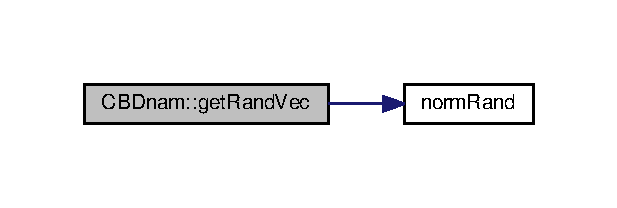
\includegraphics[width=296pt]{classCBDnam_a3f3175ac827dba969004309109e8e70c_cgraph}
\end{center}
\end{figure}


\hypertarget{classCBDnam_abee84e16de486d43f3bed18117c7031d}{\index{C\-B\-Dnam@{C\-B\-Dnam}!init\-Constants@{init\-Constants}}
\index{init\-Constants@{init\-Constants}!CBDnam@{C\-B\-Dnam}}
\subsubsection[{init\-Constants}]{\setlength{\rightskip}{0pt plus 5cm}void C\-B\-Dnam\-::init\-Constants (
\begin{DoxyParamCaption}
\item[{int}]{n\-Mol\-Type}
\end{DoxyParamCaption}
)\hspace{0.3cm}{\ttfamily [static]}}}\label{classCBDnam_abee84e16de486d43f3bed18117c7031d}
Initialize constants for a nam run \hypertarget{classCBDnam_a07205701ed2267dc0457a4d621bb8aa8}{\index{C\-B\-Dnam@{C\-B\-Dnam}!run@{run}}
\index{run@{run}!CBDnam@{C\-B\-Dnam}}
\subsubsection[{run}]{\setlength{\rightskip}{0pt plus 5cm}{\bf C\-B\-Dnam\-::\-S\-T\-A\-T\-U\-S} C\-B\-Dnam\-::run (
\begin{DoxyParamCaption}
\item[{int \&}]{scount, }
\item[{char $\ast$}]{runname}
\end{DoxyParamCaption}
)}}\label{classCBDnam_a07205701ed2267dc0457a4d621bb8aa8}
B\-Dnam run function\-: generally what happens here\-:
\begin{DoxyEnumerate}
\item two molecules position and orientation are set
\item one is in the center, the other at some random distance from it in the simulation box both have random orientations
\item Then the timestep is set, and for the time that they are not S\-T\-U\-C\-K, D\-O\-C\-K\-E\-D or E\-S\-C\-A\-P\-E\-D, a B\-D simulation advances 
\end{DoxyEnumerate}

Here is the call graph for this function\-:\nopagebreak
\begin{figure}[H]
\begin{center}
\leavevmode
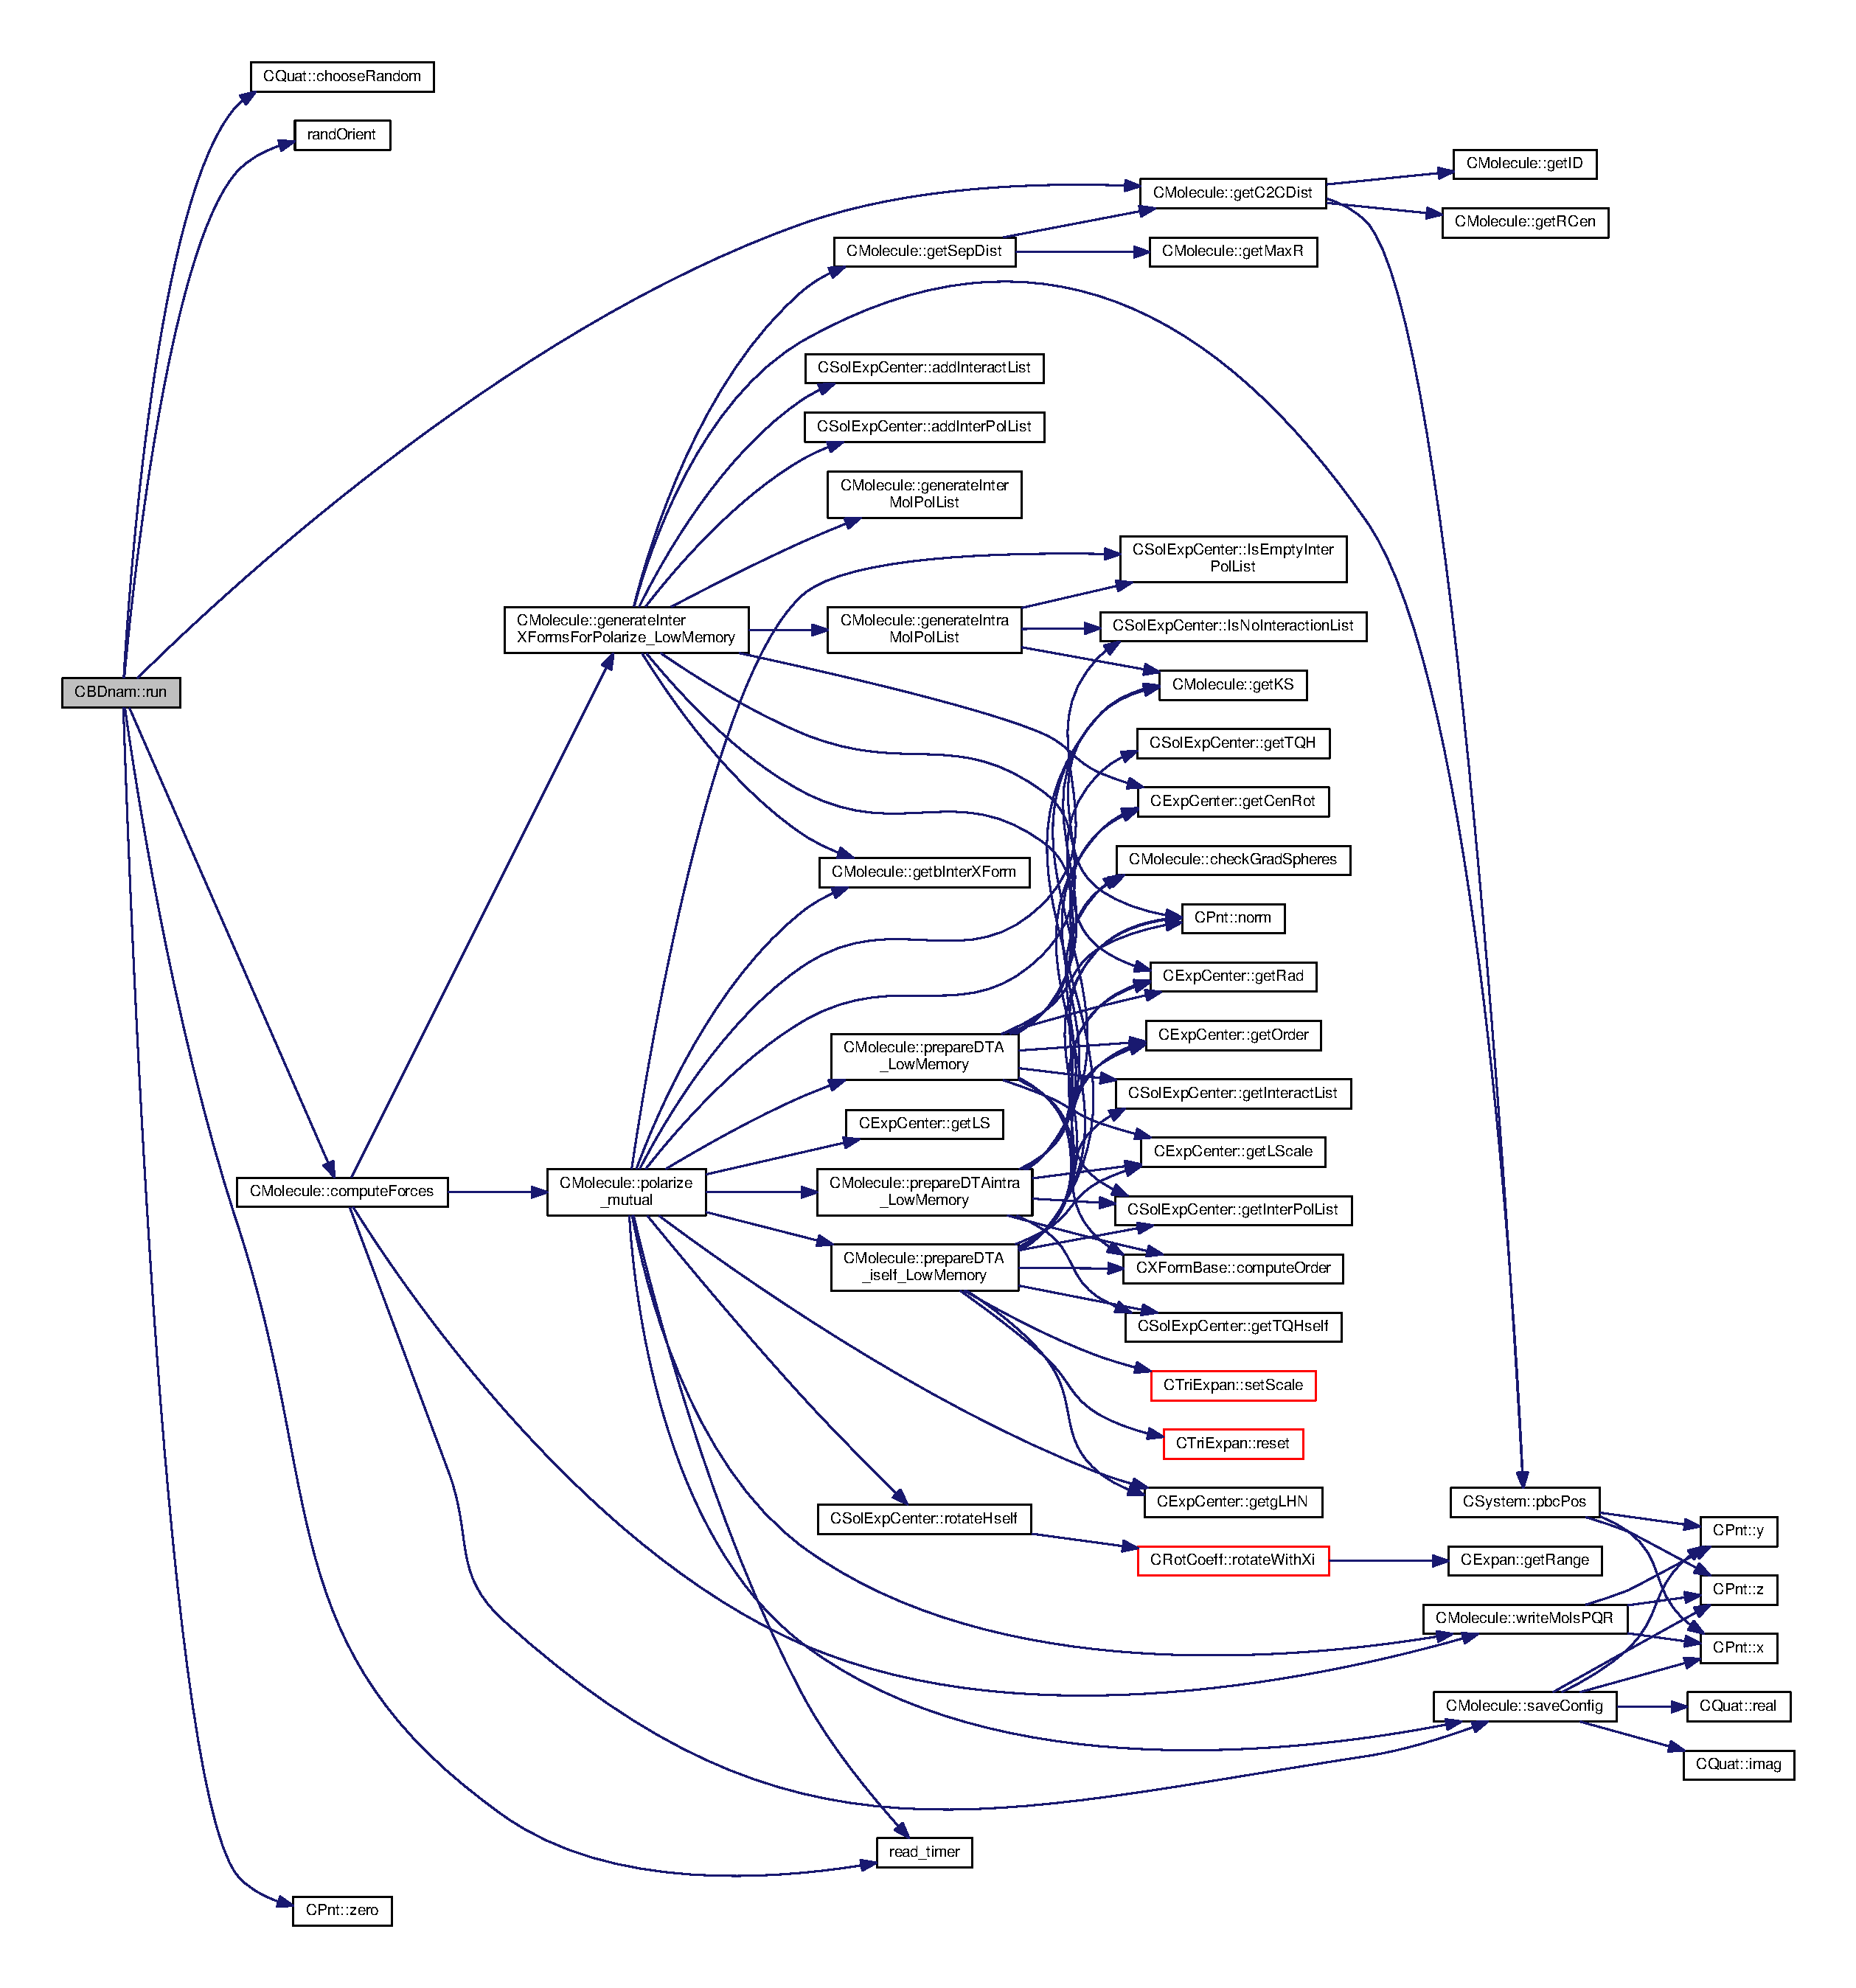
\includegraphics[width=350pt]{classCBDnam_a07205701ed2267dc0457a4d621bb8aa8_cgraph}
\end{center}
\end{figure}




\subsection{Member Data Documentation}
\hypertarget{classCBDnam_a0ca7d3cb1a694687bc249cb90bd549f0}{\index{C\-B\-Dnam@{C\-B\-Dnam}!S\-T\-A\-T\-U\-S\-\_\-\-S\-T\-R\-I\-N\-G@{S\-T\-A\-T\-U\-S\-\_\-\-S\-T\-R\-I\-N\-G}}
\index{S\-T\-A\-T\-U\-S\-\_\-\-S\-T\-R\-I\-N\-G@{S\-T\-A\-T\-U\-S\-\_\-\-S\-T\-R\-I\-N\-G}!CBDnam@{C\-B\-Dnam}}
\subsubsection[{S\-T\-A\-T\-U\-S\-\_\-\-S\-T\-R\-I\-N\-G}]{\setlength{\rightskip}{0pt plus 5cm}const char C\-B\-Dnam\-::\-S\-T\-A\-T\-U\-S\-\_\-\-S\-T\-R\-I\-N\-G = \{\char`\"{}E\-S\-C\-A\-P\-E\-D\char`\"{}, \char`\"{}{\bf D\-O\-C\-K\-E\-D}\char`\"{}, \char`\"{}{\bf R\-U\-N\-N\-I\-N\-G}\char`\"{}, \char`\"{}{\bf S\-T\-U\-C\-K}\char`\"{}\}\hspace{0.3cm}{\ttfamily [static]}}}\label{classCBDnam_a0ca7d3cb1a694687bc249cb90bd549f0}


The documentation for this class was generated from the following files\-:\begin{DoxyCompactItemize}
\item 
\hyperlink{BDnam_8h}{B\-Dnam.\-h}\item 
\hyperlink{BDnam_8cpp}{B\-Dnam.\-cpp}\end{DoxyCompactItemize}

\hypertarget{classCContact}{\section{C\-Contact Class Reference}
\label{classCContact}\index{C\-Contact@{C\-Contact}}
}


The \hyperlink{classCContact}{C\-Contact} class.  




{\ttfamily \#include $<$contact.\-h$>$}

\subsection*{Public Member Functions}
\begin{DoxyCompactItemize}
\item 
\hyperlink{classCContact_a2e2b9fcbde1245b12dfbf5c525f2e2f2}{C\-Contact} (int id1, int id2, \hyperlink{util_8h_a5821460e95a0800cf9f24c38915cbbde}{R\-E\-A\-L} dist=\hyperlink{classCContact_ad644f8a39a8f8778cac26a8c7a56e7fa}{S\-E\-P\-D\-I\-S\-T})
\begin{DoxyCompactList}\small\item\em The \hyperlink{classCContact}{C\-Contact} class constructor. \end{DoxyCompactList}\item 
int \hyperlink{classCContact_a8e28fd0d482ba1aadff37f41895e1027}{get\-I\-D1} () const 
\item 
int \hyperlink{classCContact_a7120e6624807063f3a4a40b2dd3228cf}{get\-I\-D2} () const 
\item 
double \hyperlink{classCContact_a78ffd6a0dff43ba55c25aa05a9258302}{get\-Dist} () const 
\end{DoxyCompactItemize}
\subsection*{Static Public Member Functions}
\begin{DoxyCompactItemize}
\item 
static void \hyperlink{classCContact_a868386a669900e33db303fa530b4fe65}{set\-Sep\-Dist} (\hyperlink{util_8h_a5821460e95a0800cf9f24c38915cbbde}{R\-E\-A\-L} dist)
\end{DoxyCompactItemize}
\subsection*{Static Public Attributes}
\begin{DoxyCompactItemize}
\item 
static \hyperlink{util_8h_a5821460e95a0800cf9f24c38915cbbde}{R\-E\-A\-L} \hyperlink{classCContact_ad644f8a39a8f8778cac26a8c7a56e7fa}{S\-E\-P\-D\-I\-S\-T} = 2.\-0
\begin{DoxyCompactList}\small\item\em A separation distance. \end{DoxyCompactList}\end{DoxyCompactItemize}


\subsection{Detailed Description}
The \hyperlink{classCContact}{C\-Contact} class. 

The class that contains information about atomic molecule contacts 

\subsection{Constructor \& Destructor Documentation}
\hypertarget{classCContact_a2e2b9fcbde1245b12dfbf5c525f2e2f2}{\index{C\-Contact@{C\-Contact}!C\-Contact@{C\-Contact}}
\index{C\-Contact@{C\-Contact}!CContact@{C\-Contact}}
\subsubsection[{C\-Contact}]{\setlength{\rightskip}{0pt plus 5cm}C\-Contact\-::\-C\-Contact (
\begin{DoxyParamCaption}
\item[{int}]{id1, }
\item[{int}]{id2, }
\item[{{\bf R\-E\-A\-L}}]{dist = {\ttfamily {\bf S\-E\-P\-D\-I\-S\-T}}}
\end{DoxyParamCaption}
)\hspace{0.3cm}{\ttfamily [inline]}}}\label{classCContact_a2e2b9fcbde1245b12dfbf5c525f2e2f2}


The \hyperlink{classCContact}{C\-Contact} class constructor. 

The constructor that creates a \hyperlink{classCContact}{C\-Contact} object 
\begin{DoxyParams}{Parameters}
{\em id1} & the integer I\-D of atom on molecule 1 in contact \\
\hline
{\em id2} & the integer I\-D of atom on molecule 2 in contact \\
\hline
{\em dist} & a floating point of the physical distance between the two atoms when in contact \\
\hline
\end{DoxyParams}


\subsection{Member Function Documentation}
\hypertarget{classCContact_a78ffd6a0dff43ba55c25aa05a9258302}{\index{C\-Contact@{C\-Contact}!get\-Dist@{get\-Dist}}
\index{get\-Dist@{get\-Dist}!CContact@{C\-Contact}}
\subsubsection[{get\-Dist}]{\setlength{\rightskip}{0pt plus 5cm}double C\-Contact\-::get\-Dist (
\begin{DoxyParamCaption}
{}
\end{DoxyParamCaption}
) const\hspace{0.3cm}{\ttfamily [inline]}}}\label{classCContact_a78ffd6a0dff43ba55c25aa05a9258302}
\hypertarget{classCContact_a8e28fd0d482ba1aadff37f41895e1027}{\index{C\-Contact@{C\-Contact}!get\-I\-D1@{get\-I\-D1}}
\index{get\-I\-D1@{get\-I\-D1}!CContact@{C\-Contact}}
\subsubsection[{get\-I\-D1}]{\setlength{\rightskip}{0pt plus 5cm}int C\-Contact\-::get\-I\-D1 (
\begin{DoxyParamCaption}
{}
\end{DoxyParamCaption}
) const\hspace{0.3cm}{\ttfamily [inline]}}}\label{classCContact_a8e28fd0d482ba1aadff37f41895e1027}
\hypertarget{classCContact_a7120e6624807063f3a4a40b2dd3228cf}{\index{C\-Contact@{C\-Contact}!get\-I\-D2@{get\-I\-D2}}
\index{get\-I\-D2@{get\-I\-D2}!CContact@{C\-Contact}}
\subsubsection[{get\-I\-D2}]{\setlength{\rightskip}{0pt plus 5cm}int C\-Contact\-::get\-I\-D2 (
\begin{DoxyParamCaption}
{}
\end{DoxyParamCaption}
) const\hspace{0.3cm}{\ttfamily [inline]}}}\label{classCContact_a7120e6624807063f3a4a40b2dd3228cf}
\hypertarget{classCContact_a868386a669900e33db303fa530b4fe65}{\index{C\-Contact@{C\-Contact}!set\-Sep\-Dist@{set\-Sep\-Dist}}
\index{set\-Sep\-Dist@{set\-Sep\-Dist}!CContact@{C\-Contact}}
\subsubsection[{set\-Sep\-Dist}]{\setlength{\rightskip}{0pt plus 5cm}static void C\-Contact\-::set\-Sep\-Dist (
\begin{DoxyParamCaption}
\item[{{\bf R\-E\-A\-L}}]{dist}
\end{DoxyParamCaption}
)\hspace{0.3cm}{\ttfamily [inline]}, {\ttfamily [static]}}}\label{classCContact_a868386a669900e33db303fa530b4fe65}


\subsection{Member Data Documentation}
\hypertarget{classCContact_ad644f8a39a8f8778cac26a8c7a56e7fa}{\index{C\-Contact@{C\-Contact}!S\-E\-P\-D\-I\-S\-T@{S\-E\-P\-D\-I\-S\-T}}
\index{S\-E\-P\-D\-I\-S\-T@{S\-E\-P\-D\-I\-S\-T}!CContact@{C\-Contact}}
\subsubsection[{S\-E\-P\-D\-I\-S\-T}]{\setlength{\rightskip}{0pt plus 5cm}double C\-Contact\-::\-S\-E\-P\-D\-I\-S\-T = 2.\-0\hspace{0.3cm}{\ttfamily [static]}}}\label{classCContact_ad644f8a39a8f8778cac26a8c7a56e7fa}


A separation distance. 



The documentation for this class was generated from the following files\-:\begin{DoxyCompactItemize}
\item 
\hyperlink{contact_8h}{contact.\-h}\item 
\hyperlink{contact_8cpp}{contact.\-cpp}\item 
\hyperlink{findContacts_8cpp}{find\-Contacts.\-cpp}\end{DoxyCompactItemize}

\hypertarget{classCExpan}{\section{C\-Expan Class Reference}
\label{classCExpan}\index{C\-Expan@{C\-Expan}}
}


{\ttfamily \#include $<$expansion.\-h$>$}



Inheritance diagram for C\-Expan\-:\nopagebreak
\begin{figure}[H]
\begin{center}
\leavevmode
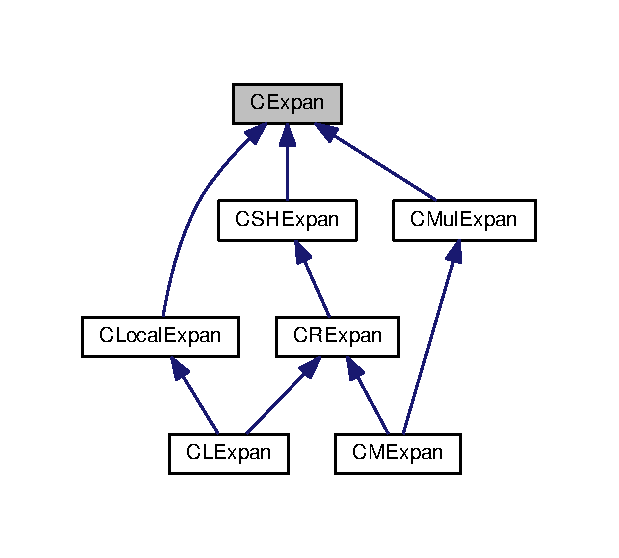
\includegraphics[width=297pt]{classCExpan__inherit__graph}
\end{center}
\end{figure}


Collaboration diagram for C\-Expan\-:\nopagebreak
\begin{figure}[H]
\begin{center}
\leavevmode
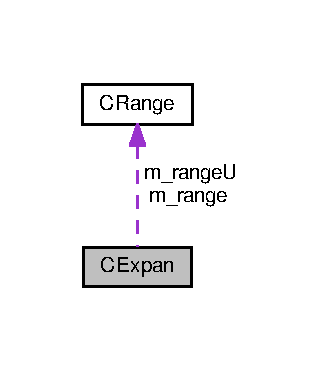
\includegraphics[width=155pt]{classCExpan__coll__graph}
\end{center}
\end{figure}
\subsection*{Public Member Functions}
\begin{DoxyCompactItemize}
\item 
\hyperlink{classCExpan_abc75d2ba91c4eedfa5661ab40dc768e8}{C\-Expan} (int p=0, \hyperlink{util_8h_a5821460e95a0800cf9f24c38915cbbde}{R\-E\-A\-L} scale=1.\-0)
\item 
\hyperlink{classCExpan_a7b7603483a63741e1fa4a0f8dfee9588}{C\-Expan} (const \hyperlink{classCRange}{C\-Range} \&R, double scale=1.\-0)
\item 
void \hyperlink{classCExpan_aa72484521209a587e90bc46ed204a59a}{copy} (const \hyperlink{classCExpan}{C\-Expan} \&M, const int p)
\item 
void \hyperlink{classCExpan_acc9b0757c5c8ce7f30a3b2dca9559128}{copy\-\_\-p} (const \hyperlink{classCExpan}{C\-Expan} \&M, const int p)
\item 
\hyperlink{classCExpan_adc9fc140dbe8c422c568d0c9db0114e2}{C\-Expan} (const double $\ast$v, const \hyperlink{classCRange}{C\-Range} \&R, double scale=1.\-0)
\item 
\hyperlink{classCExpan_a723a9f25b0c284fea509e7a5bdd76ce0}{C\-Expan} (const vector$<$ \hyperlink{util_8h_a5821460e95a0800cf9f24c38915cbbde}{R\-E\-A\-L} $>$ \&M, const \hyperlink{classCRange}{C\-Range} \&R, double scale=1.\-0)
\item 
\hyperlink{classCExpan_a896dcdd00c40227c6b2299c7859dcb24}{C\-Expan} (const double $\ast$v, int m, int i, const \hyperlink{classCRange}{C\-Range} \&R, double scale=1.\-0)
\item 
\hyperlink{classCExpan}{C\-Expan} \& \hyperlink{classCExpan_a2d3ed1e4ae47409a06009cba50d74024}{operator=} (const \hyperlink{classCExpan}{C\-Expan} \&M)
\item 
\hyperlink{classCExpan_a6ac0c2ff3c5692067ce40c16e4c564e2}{C\-Expan} (const \hyperlink{classCExpan}{C\-Expan} \&M)
\item 
void \hyperlink{classCExpan_a5c603986cd9b905dafefd83370a89d8c}{recip} ()
\item 
void \hyperlink{classCExpan_a8a6140fec725f418de3895bbf954e830}{reset} (const \hyperlink{classCRange}{C\-Range} \&R)
\item 
void \hyperlink{classCExpan_a0804b9108e1b448fe6fd101b338f1814}{clear} ()
\item 
void \hyperlink{classCExpan_ab384e5b3d427707106d655d8d9585ecc}{set\-Vector} (const \hyperlink{util_8h_a5821460e95a0800cf9f24c38915cbbde}{R\-E\-A\-L} $\ast$M, int len)
\item 
\hyperlink{util_8h_a5821460e95a0800cf9f24c38915cbbde}{R\-E\-A\-L} \hyperlink{classCExpan_a320228753bd00097b31017fbbc0564ca}{operator\mbox{[}$\,$\mbox{]}} (int i) const 
\item 
\hyperlink{util_8h_a5821460e95a0800cf9f24c38915cbbde}{R\-E\-A\-L} \& \hyperlink{classCExpan_af4292c53f4cdd9856b5e42c26e1231ce}{operator\mbox{[}$\,$\mbox{]}} (int i)
\item 
\hyperlink{util_8h_a0ef19d29521fc1e3356ea268ba175cfc}{Complex} \hyperlink{classCExpan_a4ffcff1d5e9bb8e93587f86871808fde}{comp} (int n, int m) const 
\item 
\hyperlink{util_8h_a5821460e95a0800cf9f24c38915cbbde}{R\-E\-A\-L} \hyperlink{classCExpan_ad161884680e4926b1425d65c26239610}{operator()} (int n, int mm) const 
\item 
\hyperlink{util_8h_a5821460e95a0800cf9f24c38915cbbde}{R\-E\-A\-L} \& \hyperlink{classCExpan_a72b76c1c1448f9fd55f384e20443e821}{operator()} (int n, int mm)
\item 
const vector$<$ \hyperlink{util_8h_a5821460e95a0800cf9f24c38915cbbde}{R\-E\-A\-L} $>$ \& \hyperlink{classCExpan_ad7f40483437c9d78f5353843b381ddd8}{get\-Vector} () const 
\item 
const vector$<$ \hyperlink{util_8h_a5821460e95a0800cf9f24c38915cbbde}{R\-E\-A\-L} $>$ \hyperlink{classCExpan_aea4a9b2183cf94572429330c6a3cdb54}{get\-Vector} (int p) const 
\item 
double \hyperlink{classCExpan_a849c5d81bbc37ea52dd660d5950f264c}{get\-Scale} () const 
\item 
void \hyperlink{classCExpan_aa36e147d92fd44b430f8962b2f358e8d}{set\-Scale} (double scale)
\item 
\hyperlink{classCExpan}{C\-Expan} \& \hyperlink{classCExpan_a6310d334b4ed3b3edb9cde827092c5b3}{operator$\ast$=} (const \hyperlink{util_8h_a5821460e95a0800cf9f24c38915cbbde}{R\-E\-A\-L} s)
\item 
\hyperlink{classCExpan}{C\-Expan} \& \hyperlink{classCExpan_a862fc4cbc571689e4e0e1e5ba74f990f}{operator$\ast$=} (const \hyperlink{util_8h_a5821460e95a0800cf9f24c38915cbbde}{R\-E\-A\-L} $\ast$C)
\item 
\hyperlink{classCExpan}{C\-Expan} \& \hyperlink{classCExpan_a25b49493b32656ff9caeeecd74566170}{operator+=} (const \hyperlink{classCExpan}{C\-Expan} \&E)
\item 
\hyperlink{classCExpan}{C\-Expan} \& \hyperlink{classCExpan_ae438fdfbb6573bb8036bd3413fbb1996}{operator-\/=} (const \hyperlink{classCExpan}{C\-Expan} \&E)
\item 
\hyperlink{classCExpan}{C\-Expan} \hyperlink{classCExpan_a3dd0f73609a7ae52b9203a8aed56b481}{operator-\/} () const 
\item 
void \hyperlink{classCExpan_aa4ce064fc22518c150cabbbe15bba67f}{set\-Range} (const \hyperlink{classCRange}{C\-Range} \&range)
\item 
void \hyperlink{classCExpan_ac044e829b5ac153720826b7d29c32afd}{set\-Range} (int p)
\item 
virtual const \hyperlink{classCRange}{C\-Range} \& \hyperlink{classCExpan_a8603cbb7c8f67972e825d583711d59fd}{get\-Range} () const 
\item 
int \hyperlink{classCExpan_a3f11252425c30b1ec0e81cde708d0672}{length} () const 
\item 
void \hyperlink{classCExpan_ae1c99eafb59e32ef4bf81ab6ab355d23}{output} (int p1, int p2)
\item 
void \hyperlink{classCExpan_aa394bd74d23ce1ef31185026b82a7016}{output} ()
\item 
void \hyperlink{classCExpan_ad5f9d12cd91388ca3530732c6ce16e84}{output\-Complex} (\hyperlink{util_8h_a5821460e95a0800cf9f24c38915cbbde}{R\-E\-A\-L} fact=1.\-0) const 
\item 
void \hyperlink{classCExpan_adc5e166d57954d68c63558750d4f3a00}{save\-Undo} ()
\item 
void \hyperlink{classCExpan_a61536819576535d2eb64f977b28134a0}{undo} ()
\item 
bool \hyperlink{classCExpan_aa3f0da342adec3dc09c9d8def24e5e0a}{is\-Blownup} ()
\end{DoxyCompactItemize}
\subsection*{Static Public Member Functions}
\begin{DoxyCompactItemize}
\item 
static void \hyperlink{classCExpan_a510850651229135cf89ff9f83a30c9d5}{init\-Constants} ()
\begin{DoxyCompactList}\small\item\em \hyperlink{classCExpan}{C\-Expan} init\-Constants function. \end{DoxyCompactList}\item 
static \hyperlink{util_8h_a5821460e95a0800cf9f24c38915cbbde}{R\-E\-A\-L} \hyperlink{classCExpan_ab048f9434fdfccf8289375a1b689393f}{choose\-Scale} (const vector$<$ \hyperlink{classCPnt}{C\-Pnt} $>$ \&pos)
\item 
static \hyperlink{util_8h_a5821460e95a0800cf9f24c38915cbbde}{R\-E\-A\-L} \hyperlink{classCExpan_a1b350268475522736c8a85065093a0ca}{choose\-Scale} (double min, double max)
\item 
static \hyperlink{util_8h_a5821460e95a0800cf9f24c38915cbbde}{R\-E\-A\-L} \hyperlink{classCExpan_a2d6598330609237ddb956f14705c264a}{compute\-Dev} (const \hyperlink{classCExpan}{C\-Expan} \&M1, const \hyperlink{classCExpan}{C\-Expan} \&M2)
\end{DoxyCompactItemize}
\subsection*{Static Public Attributes}
\begin{DoxyCompactItemize}
\item 
static int \hyperlink{classCExpan_a0e7564a3c13370795a342ce9d4b263a7}{I\-D\-X} \mbox{[}2 $\ast$\hyperlink{expansion_8h_ac23f9c13c5d07d9ce386f7a830c35e5a}{N\-\_\-\-P\-O\-L\-E\-S}+1\mbox{]}
\begin{DoxyCompactList}\small\item\em Contains the index for first position of constants of every n level. \end{DoxyCompactList}\item 
static \hyperlink{util_8h_a5821460e95a0800cf9f24c38915cbbde}{R\-E\-A\-L} \hyperlink{classCExpan_aa5282327718d2c6dbff1ef2fbc0fe4dd}{S\-Q\-R\-T2} = sqrt( 1.\-0 )
\item 
static \hyperlink{util_8h_a5821460e95a0800cf9f24c38915cbbde}{R\-E\-A\-L} \hyperlink{classCExpan_a4b0d1b36d98257b16600f1ffc6d20ba3}{I\-S\-Q\-R\-T2} = sqrt( 1.\-0 )
\end{DoxyCompactItemize}
\subsection*{Protected Attributes}
\begin{DoxyCompactItemize}
\item 
vector$<$ \hyperlink{util_8h_a5821460e95a0800cf9f24c38915cbbde}{R\-E\-A\-L} $>$ \hyperlink{classCExpan_a6016c7f7b961e2f69c6d7ca9daedbbf5}{m\-\_\-\-M}
\item 
vector$<$ \hyperlink{util_8h_a5821460e95a0800cf9f24c38915cbbde}{R\-E\-A\-L} $>$ \hyperlink{classCExpan_a151aff07c3667229bfa6d9d3e6e87dfc}{m\-\_\-\-M\-U}
\item 
\hyperlink{classCRange}{C\-Range} \hyperlink{classCExpan_adca887f9cd66e5e5c800a41c3e406559}{m\-\_\-range}
\begin{DoxyCompactList}\small\item\em A range object of current expansion. \end{DoxyCompactList}\item 
\hyperlink{classCRange}{C\-Range} \hyperlink{classCExpan_ae9c36d68e7ef5bdf74ad220141367792}{m\-\_\-range\-U}
\begin{DoxyCompactList}\small\item\em A saved range object of previous expansion, stored for undo. \end{DoxyCompactList}\item 
double \hyperlink{classCExpan_a4dba59941eefe0f6d70fb89f1e610d77}{m\-\_\-scale}
\item 
double \hyperlink{classCExpan_a16aade514bb13da387040369e7137aeb}{m\-\_\-scale\-U}
\end{DoxyCompactItemize}
\subsection*{Static Protected Attributes}
\begin{DoxyCompactItemize}
\item 
static \hyperlink{util_8h_a5821460e95a0800cf9f24c38915cbbde}{R\-E\-A\-L} \hyperlink{classCExpan_a1e3c0894a6550c4b01722e9741c83666}{R\-A\-T\-I\-O} = 18.\-0
\end{DoxyCompactItemize}
\subsection*{Friends}
\begin{DoxyCompactItemize}
\item 
bool \hyperlink{classCExpan_a35fefc436ee691468cdc7390ec783400}{Is\-Scale\-Equal} (const \hyperlink{classCExpan}{C\-Expan} \&M1, const \hyperlink{classCExpan}{C\-Expan} \&M2)
\item 
\hyperlink{classCExpan}{C\-Expan} \hyperlink{classCExpan_af86f70797548daca1b4c94f306eb22c3}{operator+} (const \hyperlink{classCExpan}{C\-Expan} \&E1, const \hyperlink{classCExpan}{C\-Expan} \&E2)
\item 
\hyperlink{classCExpan}{C\-Expan} \hyperlink{classCExpan_a61b8986661aaa2d6f0eff5e5f2c58488}{operator-\/} (const \hyperlink{classCExpan}{C\-Expan} \&E1, const \hyperlink{classCExpan}{C\-Expan} \&E2)
\item 
double \hyperlink{classCExpan_a0dfbb05f2e29baa6aa8c097598bf9d45}{operator$\ast$} (const \hyperlink{classCExpan}{C\-Expan} \&E1, const \hyperlink{classCExpan}{C\-Expan} \&E2)
\item 
\hyperlink{classCExpan}{C\-Expan} \hyperlink{classCExpan_a70abf8064fc2c038c82602327d23da1a}{operator$\ast$} (const \hyperlink{classCExpan}{C\-Expan} \&E, const \hyperlink{util_8h_a5821460e95a0800cf9f24c38915cbbde}{R\-E\-A\-L} $\ast$C)
\item 
\hyperlink{classCExpan}{C\-Expan} \hyperlink{classCExpan_ac0b2a0b0ce2280f60412bb96aed5f3dd}{operator$\ast$} (\hyperlink{util_8h_a5821460e95a0800cf9f24c38915cbbde}{R\-E\-A\-L} s, const \hyperlink{classCExpan}{C\-Expan} \&E)
\item 
\hyperlink{util_8h_a5821460e95a0800cf9f24c38915cbbde}{R\-E\-A\-L} \hyperlink{classCExpan_a5b8852acff77a8c6c5a167d050c7cee2}{inprod\-\_\-unit\-Scale} (const \hyperlink{classCExpan}{C\-Expan} \&E1, const \hyperlink{classCExpan}{C\-Expan} \&E2)
\item 
ostream \& \hyperlink{classCExpan_adfca34b8a78f7e0647ee4113707047c4}{operator$<$$<$} (ostream \&out, const \hyperlink{classCExpan}{C\-Expan} \&p)
\end{DoxyCompactItemize}


\subsection{Detailed Description}
The \hyperlink{classCExpan}{C\-Expan} class

The \hyperlink{classCExpan}{C\-Expan} class contains information about basic expansions. 

\subsection{Constructor \& Destructor Documentation}
\hypertarget{classCExpan_abc75d2ba91c4eedfa5661ab40dc768e8}{\index{C\-Expan@{C\-Expan}!C\-Expan@{C\-Expan}}
\index{C\-Expan@{C\-Expan}!CExpan@{C\-Expan}}
\subsubsection[{C\-Expan}]{\setlength{\rightskip}{0pt plus 5cm}C\-Expan\-::\-C\-Expan (
\begin{DoxyParamCaption}
\item[{int}]{p = {\ttfamily 0}, }
\item[{{\bf R\-E\-A\-L}}]{scale = {\ttfamily 1.0}}
\end{DoxyParamCaption}
)\hspace{0.3cm}{\ttfamily [inline]}}}\label{classCExpan_abc75d2ba91c4eedfa5661ab40dc768e8}
\hypertarget{classCExpan_a7b7603483a63741e1fa4a0f8dfee9588}{\index{C\-Expan@{C\-Expan}!C\-Expan@{C\-Expan}}
\index{C\-Expan@{C\-Expan}!CExpan@{C\-Expan}}
\subsubsection[{C\-Expan}]{\setlength{\rightskip}{0pt plus 5cm}C\-Expan\-::\-C\-Expan (
\begin{DoxyParamCaption}
\item[{const {\bf C\-Range} \&}]{R, }
\item[{double}]{scale = {\ttfamily 1.0}}
\end{DoxyParamCaption}
)\hspace{0.3cm}{\ttfamily [inline]}}}\label{classCExpan_a7b7603483a63741e1fa4a0f8dfee9588}
\hypertarget{classCExpan_adc9fc140dbe8c422c568d0c9db0114e2}{\index{C\-Expan@{C\-Expan}!C\-Expan@{C\-Expan}}
\index{C\-Expan@{C\-Expan}!CExpan@{C\-Expan}}
\subsubsection[{C\-Expan}]{\setlength{\rightskip}{0pt plus 5cm}C\-Expan\-::\-C\-Expan (
\begin{DoxyParamCaption}
\item[{const double $\ast$}]{v, }
\item[{const {\bf C\-Range} \&}]{range, }
\item[{double}]{scale = {\ttfamily 1.0}}
\end{DoxyParamCaption}
)}}\label{classCExpan_adc9fc140dbe8c422c568d0c9db0114e2}
Create an expansion using the supplied coefficients. 

Here is the call graph for this function\-:\nopagebreak
\begin{figure}[H]
\begin{center}
\leavevmode
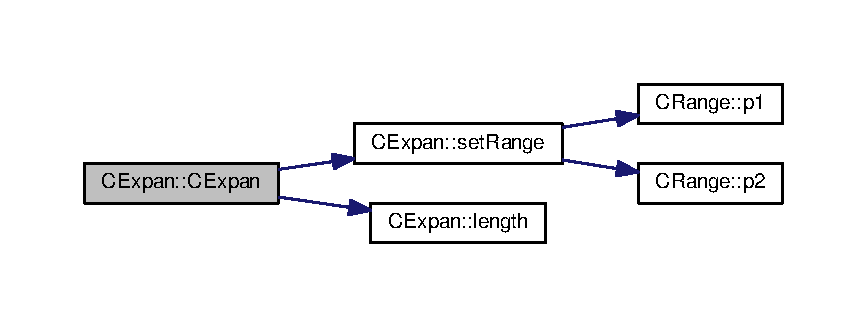
\includegraphics[width=350pt]{classCExpan_adc9fc140dbe8c422c568d0c9db0114e2_cgraph}
\end{center}
\end{figure}


\hypertarget{classCExpan_a723a9f25b0c284fea509e7a5bdd76ce0}{\index{C\-Expan@{C\-Expan}!C\-Expan@{C\-Expan}}
\index{C\-Expan@{C\-Expan}!CExpan@{C\-Expan}}
\subsubsection[{C\-Expan}]{\setlength{\rightskip}{0pt plus 5cm}C\-Expan\-::\-C\-Expan (
\begin{DoxyParamCaption}
\item[{const vector$<$ {\bf R\-E\-A\-L} $>$ \&}]{M, }
\item[{const {\bf C\-Range} \&}]{range, }
\item[{double}]{scale = {\ttfamily 1.0}}
\end{DoxyParamCaption}
)}}\label{classCExpan_a723a9f25b0c284fea509e7a5bdd76ce0}
Create an expansion using the supplied coefficients. 

Here is the call graph for this function\-:\nopagebreak
\begin{figure}[H]
\begin{center}
\leavevmode
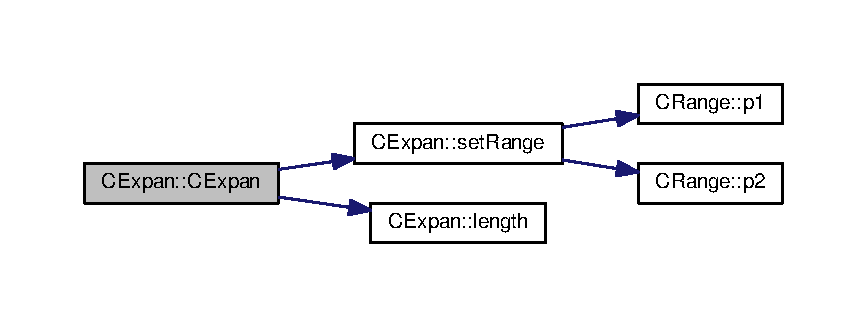
\includegraphics[width=350pt]{classCExpan_a723a9f25b0c284fea509e7a5bdd76ce0_cgraph}
\end{center}
\end{figure}


\hypertarget{classCExpan_a896dcdd00c40227c6b2299c7859dcb24}{\index{C\-Expan@{C\-Expan}!C\-Expan@{C\-Expan}}
\index{C\-Expan@{C\-Expan}!CExpan@{C\-Expan}}
\subsubsection[{C\-Expan}]{\setlength{\rightskip}{0pt plus 5cm}C\-Expan\-::\-C\-Expan (
\begin{DoxyParamCaption}
\item[{const double $\ast$}]{A, }
\item[{int}]{m, }
\item[{int}]{i, }
\item[{const {\bf C\-Range} \&}]{range, }
\item[{double}]{scale = {\ttfamily 1.0}}
\end{DoxyParamCaption}
)}}\label{classCExpan_a896dcdd00c40227c6b2299c7859dcb24}
Create an expansion using the supplied coefficients in the i-\/th row of the column-\/major matrix 

Here is the call graph for this function\-:\nopagebreak
\begin{figure}[H]
\begin{center}
\leavevmode
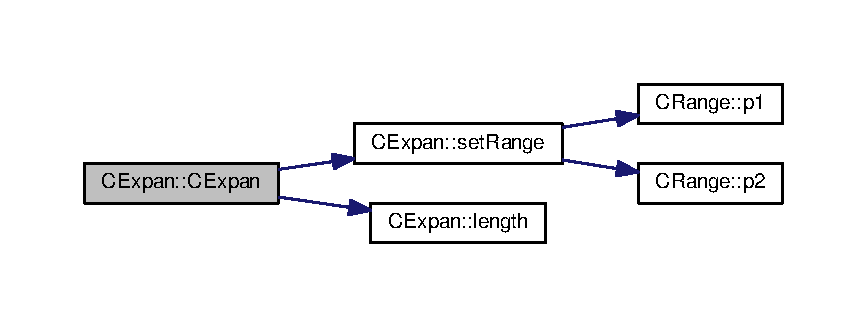
\includegraphics[width=350pt]{classCExpan_a896dcdd00c40227c6b2299c7859dcb24_cgraph}
\end{center}
\end{figure}


\hypertarget{classCExpan_a6ac0c2ff3c5692067ce40c16e4c564e2}{\index{C\-Expan@{C\-Expan}!C\-Expan@{C\-Expan}}
\index{C\-Expan@{C\-Expan}!CExpan@{C\-Expan}}
\subsubsection[{C\-Expan}]{\setlength{\rightskip}{0pt plus 5cm}C\-Expan\-::\-C\-Expan (
\begin{DoxyParamCaption}
\item[{const {\bf C\-Expan} \&}]{M}
\end{DoxyParamCaption}
)\hspace{0.3cm}{\ttfamily [inline]}}}\label{classCExpan_a6ac0c2ff3c5692067ce40c16e4c564e2}


\subsection{Member Function Documentation}
\hypertarget{classCExpan_ab048f9434fdfccf8289375a1b689393f}{\index{C\-Expan@{C\-Expan}!choose\-Scale@{choose\-Scale}}
\index{choose\-Scale@{choose\-Scale}!CExpan@{C\-Expan}}
\subsubsection[{choose\-Scale}]{\setlength{\rightskip}{0pt plus 5cm}double C\-Expan\-::choose\-Scale (
\begin{DoxyParamCaption}
\item[{const vector$<$ {\bf C\-Pnt} $>$ \&}]{pos}
\end{DoxyParamCaption}
)\hspace{0.3cm}{\ttfamily [static]}}}\label{classCExpan_ab048f9434fdfccf8289375a1b689393f}
Choose an appropriate scaling factor for the expansion based on the given set of charge positions \hypertarget{classCExpan_a1b350268475522736c8a85065093a0ca}{\index{C\-Expan@{C\-Expan}!choose\-Scale@{choose\-Scale}}
\index{choose\-Scale@{choose\-Scale}!CExpan@{C\-Expan}}
\subsubsection[{choose\-Scale}]{\setlength{\rightskip}{0pt plus 5cm}double C\-Expan\-::choose\-Scale (
\begin{DoxyParamCaption}
\item[{double}]{min, }
\item[{double}]{max}
\end{DoxyParamCaption}
)\hspace{0.3cm}{\ttfamily [static]}}}\label{classCExpan_a1b350268475522736c8a85065093a0ca}
Choose an appropriate scaling factor for the expansion based on min and max distance of the charges from the center \hypertarget{classCExpan_a0804b9108e1b448fe6fd101b338f1814}{\index{C\-Expan@{C\-Expan}!clear@{clear}}
\index{clear@{clear}!CExpan@{C\-Expan}}
\subsubsection[{clear}]{\setlength{\rightskip}{0pt plus 5cm}void C\-Expan\-::clear (
\begin{DoxyParamCaption}
{}
\end{DoxyParamCaption}
)\hspace{0.3cm}{\ttfamily [inline]}}}\label{classCExpan_a0804b9108e1b448fe6fd101b338f1814}
\hypertarget{classCExpan_a4ffcff1d5e9bb8e93587f86871808fde}{\index{C\-Expan@{C\-Expan}!comp@{comp}}
\index{comp@{comp}!CExpan@{C\-Expan}}
\subsubsection[{comp}]{\setlength{\rightskip}{0pt plus 5cm}{\bf Complex} C\-Expan\-::comp (
\begin{DoxyParamCaption}
\item[{int}]{n, }
\item[{int}]{m}
\end{DoxyParamCaption}
) const\hspace{0.3cm}{\ttfamily [inline]}}}\label{classCExpan_a4ffcff1d5e9bb8e93587f86871808fde}
\hypertarget{classCExpan_a2d6598330609237ddb956f14705c264a}{\index{C\-Expan@{C\-Expan}!compute\-Dev@{compute\-Dev}}
\index{compute\-Dev@{compute\-Dev}!CExpan@{C\-Expan}}
\subsubsection[{compute\-Dev}]{\setlength{\rightskip}{0pt plus 5cm}{\bf R\-E\-A\-L} C\-Expan\-::compute\-Dev (
\begin{DoxyParamCaption}
\item[{const {\bf C\-Expan} \&}]{M1, }
\item[{const {\bf C\-Expan} \&}]{M2}
\end{DoxyParamCaption}
)\hspace{0.3cm}{\ttfamily [inline]}, {\ttfamily [static]}}}\label{classCExpan_a2d6598330609237ddb956f14705c264a}


Here is the call graph for this function\-:\nopagebreak
\begin{figure}[H]
\begin{center}
\leavevmode
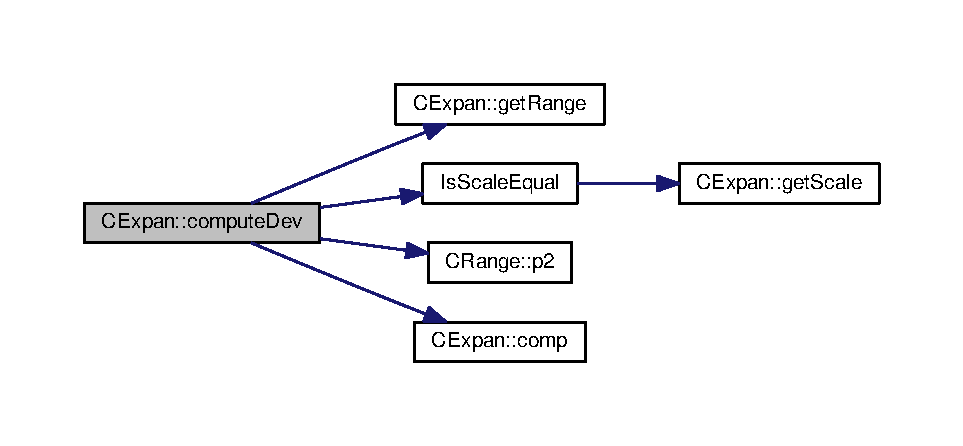
\includegraphics[width=350pt]{classCExpan_a2d6598330609237ddb956f14705c264a_cgraph}
\end{center}
\end{figure}


\hypertarget{classCExpan_aa72484521209a587e90bc46ed204a59a}{\index{C\-Expan@{C\-Expan}!copy@{copy}}
\index{copy@{copy}!CExpan@{C\-Expan}}
\subsubsection[{copy}]{\setlength{\rightskip}{0pt plus 5cm}void C\-Expan\-::copy (
\begin{DoxyParamCaption}
\item[{const {\bf C\-Expan} \&}]{M, }
\item[{const int}]{p}
\end{DoxyParamCaption}
)\hspace{0.3cm}{\ttfamily [inline]}}}\label{classCExpan_aa72484521209a587e90bc46ed204a59a}


Here is the call graph for this function\-:\nopagebreak
\begin{figure}[H]
\begin{center}
\leavevmode
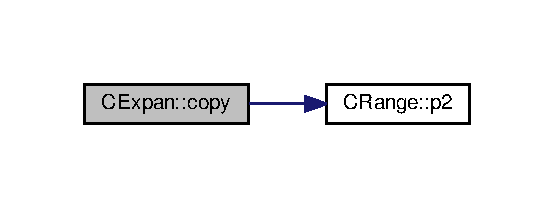
\includegraphics[width=266pt]{classCExpan_aa72484521209a587e90bc46ed204a59a_cgraph}
\end{center}
\end{figure}


\hypertarget{classCExpan_acc9b0757c5c8ce7f30a3b2dca9559128}{\index{C\-Expan@{C\-Expan}!copy\-\_\-p@{copy\-\_\-p}}
\index{copy\-\_\-p@{copy\-\_\-p}!CExpan@{C\-Expan}}
\subsubsection[{copy\-\_\-p}]{\setlength{\rightskip}{0pt plus 5cm}void C\-Expan\-::copy\-\_\-p (
\begin{DoxyParamCaption}
\item[{const {\bf C\-Expan} \&}]{M, }
\item[{const int}]{p}
\end{DoxyParamCaption}
)\hspace{0.3cm}{\ttfamily [inline]}}}\label{classCExpan_acc9b0757c5c8ce7f30a3b2dca9559128}


Here is the call graph for this function\-:\nopagebreak
\begin{figure}[H]
\begin{center}
\leavevmode
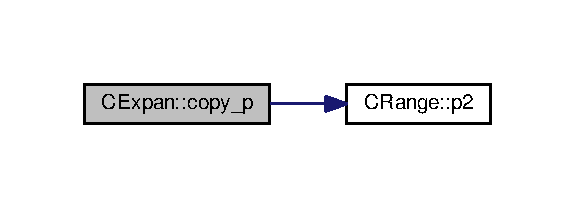
\includegraphics[width=276pt]{classCExpan_acc9b0757c5c8ce7f30a3b2dca9559128_cgraph}
\end{center}
\end{figure}


\hypertarget{classCExpan_a8603cbb7c8f67972e825d583711d59fd}{\index{C\-Expan@{C\-Expan}!get\-Range@{get\-Range}}
\index{get\-Range@{get\-Range}!CExpan@{C\-Expan}}
\subsubsection[{get\-Range}]{\setlength{\rightskip}{0pt plus 5cm}virtual const {\bf C\-Range}\& C\-Expan\-::get\-Range (
\begin{DoxyParamCaption}
{}
\end{DoxyParamCaption}
) const\hspace{0.3cm}{\ttfamily [inline]}, {\ttfamily [virtual]}}}\label{classCExpan_a8603cbb7c8f67972e825d583711d59fd}
\hypertarget{classCExpan_a849c5d81bbc37ea52dd660d5950f264c}{\index{C\-Expan@{C\-Expan}!get\-Scale@{get\-Scale}}
\index{get\-Scale@{get\-Scale}!CExpan@{C\-Expan}}
\subsubsection[{get\-Scale}]{\setlength{\rightskip}{0pt plus 5cm}double C\-Expan\-::get\-Scale (
\begin{DoxyParamCaption}
{}
\end{DoxyParamCaption}
) const\hspace{0.3cm}{\ttfamily [inline]}}}\label{classCExpan_a849c5d81bbc37ea52dd660d5950f264c}
\hypertarget{classCExpan_ad7f40483437c9d78f5353843b381ddd8}{\index{C\-Expan@{C\-Expan}!get\-Vector@{get\-Vector}}
\index{get\-Vector@{get\-Vector}!CExpan@{C\-Expan}}
\subsubsection[{get\-Vector}]{\setlength{\rightskip}{0pt plus 5cm}const vector$<${\bf R\-E\-A\-L}$>$\& C\-Expan\-::get\-Vector (
\begin{DoxyParamCaption}
{}
\end{DoxyParamCaption}
) const\hspace{0.3cm}{\ttfamily [inline]}}}\label{classCExpan_ad7f40483437c9d78f5353843b381ddd8}
\hypertarget{classCExpan_aea4a9b2183cf94572429330c6a3cdb54}{\index{C\-Expan@{C\-Expan}!get\-Vector@{get\-Vector}}
\index{get\-Vector@{get\-Vector}!CExpan@{C\-Expan}}
\subsubsection[{get\-Vector}]{\setlength{\rightskip}{0pt plus 5cm}const vector$<${\bf R\-E\-A\-L}$>$ C\-Expan\-::get\-Vector (
\begin{DoxyParamCaption}
\item[{int}]{p}
\end{DoxyParamCaption}
) const\hspace{0.3cm}{\ttfamily [inline]}}}\label{classCExpan_aea4a9b2183cf94572429330c6a3cdb54}
\hypertarget{classCExpan_a510850651229135cf89ff9f83a30c9d5}{\index{C\-Expan@{C\-Expan}!init\-Constants@{init\-Constants}}
\index{init\-Constants@{init\-Constants}!CExpan@{C\-Expan}}
\subsubsection[{init\-Constants}]{\setlength{\rightskip}{0pt plus 5cm}void C\-Expan\-::init\-Constants (
\begin{DoxyParamCaption}
{}
\end{DoxyParamCaption}
)\hspace{0.3cm}{\ttfamily [static]}}}\label{classCExpan_a510850651229135cf89ff9f83a30c9d5}


\hyperlink{classCExpan}{C\-Expan} init\-Constants function. 

This function is used to initialize system constants I\-D\-X.

\hyperlink{classCExpan}{C\-Expan} init\-Constants for initializing constants of a basic expansion. 

Reimplemented in \hyperlink{classCSHExpan_a0bc80f8710a4da0982b650089bcb94db}{C\-S\-H\-Expan}.

\hypertarget{classCExpan_aa3f0da342adec3dc09c9d8def24e5e0a}{\index{C\-Expan@{C\-Expan}!is\-Blownup@{is\-Blownup}}
\index{is\-Blownup@{is\-Blownup}!CExpan@{C\-Expan}}
\subsubsection[{is\-Blownup}]{\setlength{\rightskip}{0pt plus 5cm}bool C\-Expan\-::is\-Blownup (
\begin{DoxyParamCaption}
{}
\end{DoxyParamCaption}
)\hspace{0.3cm}{\ttfamily [inline]}}}\label{classCExpan_aa3f0da342adec3dc09c9d8def24e5e0a}
\hypertarget{classCExpan_a3f11252425c30b1ec0e81cde708d0672}{\index{C\-Expan@{C\-Expan}!length@{length}}
\index{length@{length}!CExpan@{C\-Expan}}
\subsubsection[{length}]{\setlength{\rightskip}{0pt plus 5cm}int C\-Expan\-::length (
\begin{DoxyParamCaption}
{}
\end{DoxyParamCaption}
) const\hspace{0.3cm}{\ttfamily [inline]}}}\label{classCExpan_a3f11252425c30b1ec0e81cde708d0672}
\hypertarget{classCExpan_ad161884680e4926b1425d65c26239610}{\index{C\-Expan@{C\-Expan}!operator()@{operator()}}
\index{operator()@{operator()}!CExpan@{C\-Expan}}
\subsubsection[{operator()}]{\setlength{\rightskip}{0pt plus 5cm}{\bf R\-E\-A\-L} C\-Expan\-::operator() (
\begin{DoxyParamCaption}
\item[{int}]{n, }
\item[{int}]{mm}
\end{DoxyParamCaption}
) const\hspace{0.3cm}{\ttfamily [inline]}}}\label{classCExpan_ad161884680e4926b1425d65c26239610}
\hypertarget{classCExpan_a72b76c1c1448f9fd55f384e20443e821}{\index{C\-Expan@{C\-Expan}!operator()@{operator()}}
\index{operator()@{operator()}!CExpan@{C\-Expan}}
\subsubsection[{operator()}]{\setlength{\rightskip}{0pt plus 5cm}{\bf R\-E\-A\-L} \& C\-Expan\-::operator() (
\begin{DoxyParamCaption}
\item[{int}]{n, }
\item[{int}]{mm}
\end{DoxyParamCaption}
)\hspace{0.3cm}{\ttfamily [inline]}}}\label{classCExpan_a72b76c1c1448f9fd55f384e20443e821}
\hypertarget{classCExpan_a6310d334b4ed3b3edb9cde827092c5b3}{\index{C\-Expan@{C\-Expan}!operator$\ast$=@{operator$\ast$=}}
\index{operator$\ast$=@{operator$\ast$=}!CExpan@{C\-Expan}}
\subsubsection[{operator$\ast$=}]{\setlength{\rightskip}{0pt plus 5cm}{\bf C\-Expan} \& C\-Expan\-::operator$\ast$= (
\begin{DoxyParamCaption}
\item[{const {\bf R\-E\-A\-L}}]{s}
\end{DoxyParamCaption}
)\hspace{0.3cm}{\ttfamily [inline]}}}\label{classCExpan_a6310d334b4ed3b3edb9cde827092c5b3}
\hypertarget{classCExpan_a862fc4cbc571689e4e0e1e5ba74f990f}{\index{C\-Expan@{C\-Expan}!operator$\ast$=@{operator$\ast$=}}
\index{operator$\ast$=@{operator$\ast$=}!CExpan@{C\-Expan}}
\subsubsection[{operator$\ast$=}]{\setlength{\rightskip}{0pt plus 5cm}{\bf C\-Expan} \& C\-Expan\-::operator$\ast$= (
\begin{DoxyParamCaption}
\item[{const {\bf R\-E\-A\-L} $\ast$}]{C}
\end{DoxyParamCaption}
)\hspace{0.3cm}{\ttfamily [inline]}}}\label{classCExpan_a862fc4cbc571689e4e0e1e5ba74f990f}
\hypertarget{classCExpan_a25b49493b32656ff9caeeecd74566170}{\index{C\-Expan@{C\-Expan}!operator+=@{operator+=}}
\index{operator+=@{operator+=}!CExpan@{C\-Expan}}
\subsubsection[{operator+=}]{\setlength{\rightskip}{0pt plus 5cm}{\bf C\-Expan} \& C\-Expan\-::operator+= (
\begin{DoxyParamCaption}
\item[{const {\bf C\-Expan} \&}]{E}
\end{DoxyParamCaption}
)\hspace{0.3cm}{\ttfamily [inline]}}}\label{classCExpan_a25b49493b32656ff9caeeecd74566170}


Here is the call graph for this function\-:\nopagebreak
\begin{figure}[H]
\begin{center}
\leavevmode
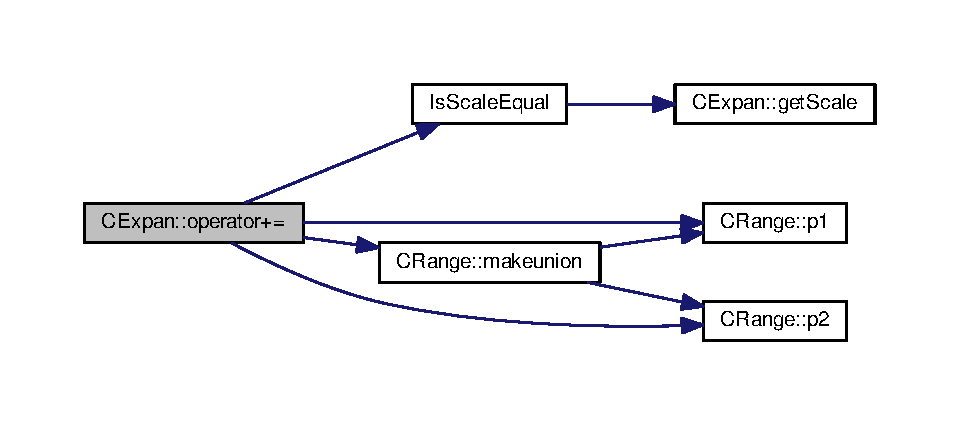
\includegraphics[width=350pt]{classCExpan_a25b49493b32656ff9caeeecd74566170_cgraph}
\end{center}
\end{figure}


\hypertarget{classCExpan_a3dd0f73609a7ae52b9203a8aed56b481}{\index{C\-Expan@{C\-Expan}!operator-\/@{operator-\/}}
\index{operator-\/@{operator-\/}!CExpan@{C\-Expan}}
\subsubsection[{operator-\/}]{\setlength{\rightskip}{0pt plus 5cm}{\bf C\-Expan} C\-Expan\-::operator-\/ (
\begin{DoxyParamCaption}
{}
\end{DoxyParamCaption}
) const\hspace{0.3cm}{\ttfamily [inline]}}}\label{classCExpan_a3dd0f73609a7ae52b9203a8aed56b481}
\hypertarget{classCExpan_ae438fdfbb6573bb8036bd3413fbb1996}{\index{C\-Expan@{C\-Expan}!operator-\/=@{operator-\/=}}
\index{operator-\/=@{operator-\/=}!CExpan@{C\-Expan}}
\subsubsection[{operator-\/=}]{\setlength{\rightskip}{0pt plus 5cm}{\bf C\-Expan} \& C\-Expan\-::operator-\/= (
\begin{DoxyParamCaption}
\item[{const {\bf C\-Expan} \&}]{E}
\end{DoxyParamCaption}
)\hspace{0.3cm}{\ttfamily [inline]}}}\label{classCExpan_ae438fdfbb6573bb8036bd3413fbb1996}


Here is the call graph for this function\-:\nopagebreak
\begin{figure}[H]
\begin{center}
\leavevmode
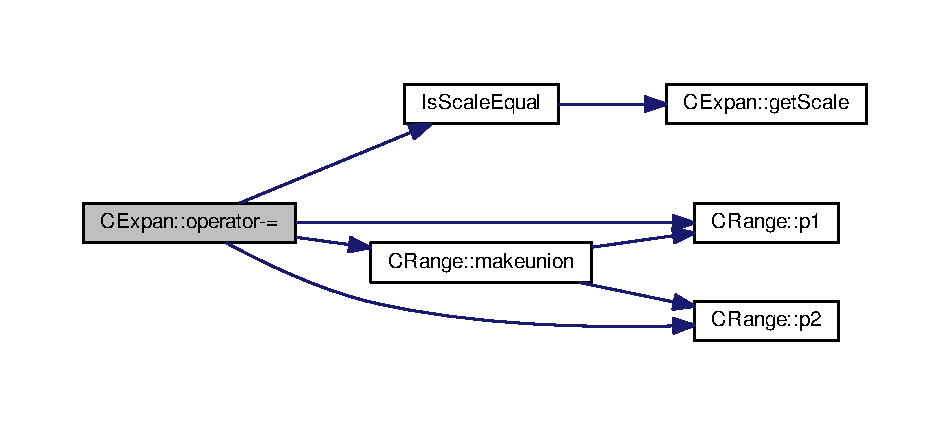
\includegraphics[width=350pt]{classCExpan_ae438fdfbb6573bb8036bd3413fbb1996_cgraph}
\end{center}
\end{figure}


\hypertarget{classCExpan_a2d3ed1e4ae47409a06009cba50d74024}{\index{C\-Expan@{C\-Expan}!operator=@{operator=}}
\index{operator=@{operator=}!CExpan@{C\-Expan}}
\subsubsection[{operator=}]{\setlength{\rightskip}{0pt plus 5cm}{\bf C\-Expan} \& C\-Expan\-::operator= (
\begin{DoxyParamCaption}
\item[{const {\bf C\-Expan} \&}]{M}
\end{DoxyParamCaption}
)}}\label{classCExpan_a2d3ed1e4ae47409a06009cba50d74024}
The expansion class = operator \hypertarget{classCExpan_a320228753bd00097b31017fbbc0564ca}{\index{C\-Expan@{C\-Expan}!operator\mbox{[}$\,$\mbox{]}@{operator[]}}
\index{operator\mbox{[}$\,$\mbox{]}@{operator[]}!CExpan@{C\-Expan}}
\subsubsection[{operator[]}]{\setlength{\rightskip}{0pt plus 5cm}{\bf R\-E\-A\-L} C\-Expan\-::operator\mbox{[}$\,$\mbox{]} (
\begin{DoxyParamCaption}
\item[{int}]{i}
\end{DoxyParamCaption}
) const\hspace{0.3cm}{\ttfamily [inline]}}}\label{classCExpan_a320228753bd00097b31017fbbc0564ca}
\hypertarget{classCExpan_af4292c53f4cdd9856b5e42c26e1231ce}{\index{C\-Expan@{C\-Expan}!operator\mbox{[}$\,$\mbox{]}@{operator[]}}
\index{operator\mbox{[}$\,$\mbox{]}@{operator[]}!CExpan@{C\-Expan}}
\subsubsection[{operator[]}]{\setlength{\rightskip}{0pt plus 5cm}{\bf R\-E\-A\-L}\& C\-Expan\-::operator\mbox{[}$\,$\mbox{]} (
\begin{DoxyParamCaption}
\item[{int}]{i}
\end{DoxyParamCaption}
)\hspace{0.3cm}{\ttfamily [inline]}}}\label{classCExpan_af4292c53f4cdd9856b5e42c26e1231ce}
\hypertarget{classCExpan_ae1c99eafb59e32ef4bf81ab6ab355d23}{\index{C\-Expan@{C\-Expan}!output@{output}}
\index{output@{output}!CExpan@{C\-Expan}}
\subsubsection[{output}]{\setlength{\rightskip}{0pt plus 5cm}void C\-Expan\-::output (
\begin{DoxyParamCaption}
\item[{int}]{p1, }
\item[{int}]{p2}
\end{DoxyParamCaption}
)}}\label{classCExpan_ae1c99eafb59e32ef4bf81ab6ab355d23}
Output expansion for a range from p1 to p2 \hypertarget{classCExpan_aa394bd74d23ce1ef31185026b82a7016}{\index{C\-Expan@{C\-Expan}!output@{output}}
\index{output@{output}!CExpan@{C\-Expan}}
\subsubsection[{output}]{\setlength{\rightskip}{0pt plus 5cm}void C\-Expan\-::output (
\begin{DoxyParamCaption}
{}
\end{DoxyParamCaption}
)\hspace{0.3cm}{\ttfamily [inline]}}}\label{classCExpan_aa394bd74d23ce1ef31185026b82a7016}


Here is the call graph for this function\-:\nopagebreak
\begin{figure}[H]
\begin{center}
\leavevmode
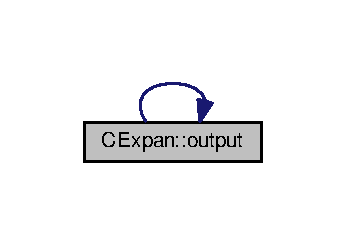
\includegraphics[width=166pt]{classCExpan_aa394bd74d23ce1ef31185026b82a7016_cgraph}
\end{center}
\end{figure}


\hypertarget{classCExpan_ad5f9d12cd91388ca3530732c6ce16e84}{\index{C\-Expan@{C\-Expan}!output\-Complex@{output\-Complex}}
\index{output\-Complex@{output\-Complex}!CExpan@{C\-Expan}}
\subsubsection[{output\-Complex}]{\setlength{\rightskip}{0pt plus 5cm}void C\-Expan\-::output\-Complex (
\begin{DoxyParamCaption}
\item[{{\bf R\-E\-A\-L}}]{fact = {\ttfamily 1.0}}
\end{DoxyParamCaption}
) const}}\label{classCExpan_ad5f9d12cd91388ca3530732c6ce16e84}
Output the complex part of an expansion class 

Here is the call graph for this function\-:\nopagebreak
\begin{figure}[H]
\begin{center}
\leavevmode
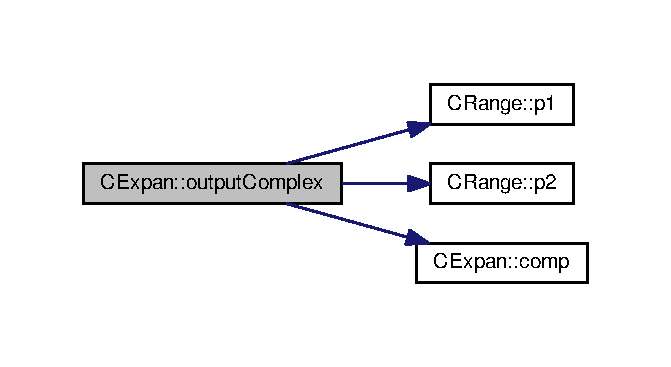
\includegraphics[width=322pt]{classCExpan_ad5f9d12cd91388ca3530732c6ce16e84_cgraph}
\end{center}
\end{figure}


\hypertarget{classCExpan_a5c603986cd9b905dafefd83370a89d8c}{\index{C\-Expan@{C\-Expan}!recip@{recip}}
\index{recip@{recip}!CExpan@{C\-Expan}}
\subsubsection[{recip}]{\setlength{\rightskip}{0pt plus 5cm}void C\-Expan\-::recip (
\begin{DoxyParamCaption}
{}
\end{DoxyParamCaption}
)\hspace{0.3cm}{\ttfamily [inline]}}}\label{classCExpan_a5c603986cd9b905dafefd83370a89d8c}
\hypertarget{classCExpan_a8a6140fec725f418de3895bbf954e830}{\index{C\-Expan@{C\-Expan}!reset@{reset}}
\index{reset@{reset}!CExpan@{C\-Expan}}
\subsubsection[{reset}]{\setlength{\rightskip}{0pt plus 5cm}void C\-Expan\-::reset (
\begin{DoxyParamCaption}
\item[{const {\bf C\-Range} \&}]{R}
\end{DoxyParamCaption}
)\hspace{0.3cm}{\ttfamily [inline]}}}\label{classCExpan_a8a6140fec725f418de3895bbf954e830}


Here is the call graph for this function\-:\nopagebreak
\begin{figure}[H]
\begin{center}
\leavevmode
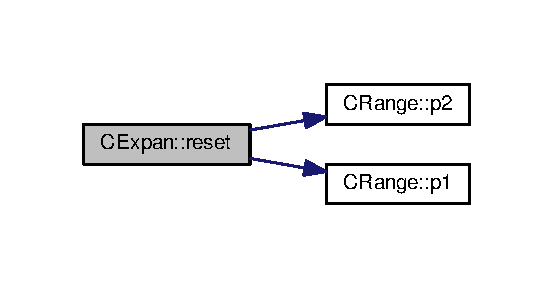
\includegraphics[width=266pt]{classCExpan_a8a6140fec725f418de3895bbf954e830_cgraph}
\end{center}
\end{figure}


\hypertarget{classCExpan_adc5e166d57954d68c63558750d4f3a00}{\index{C\-Expan@{C\-Expan}!save\-Undo@{save\-Undo}}
\index{save\-Undo@{save\-Undo}!CExpan@{C\-Expan}}
\subsubsection[{save\-Undo}]{\setlength{\rightskip}{0pt plus 5cm}void C\-Expan\-::save\-Undo (
\begin{DoxyParamCaption}
{}
\end{DoxyParamCaption}
)\hspace{0.3cm}{\ttfamily [inline]}}}\label{classCExpan_adc5e166d57954d68c63558750d4f3a00}
\hypertarget{classCExpan_aa4ce064fc22518c150cabbbe15bba67f}{\index{C\-Expan@{C\-Expan}!set\-Range@{set\-Range}}
\index{set\-Range@{set\-Range}!CExpan@{C\-Expan}}
\subsubsection[{set\-Range}]{\setlength{\rightskip}{0pt plus 5cm}void C\-Expan\-::set\-Range (
\begin{DoxyParamCaption}
\item[{const {\bf C\-Range} \&}]{range}
\end{DoxyParamCaption}
)\hspace{0.3cm}{\ttfamily [inline]}}}\label{classCExpan_aa4ce064fc22518c150cabbbe15bba67f}


Here is the call graph for this function\-:\nopagebreak
\begin{figure}[H]
\begin{center}
\leavevmode
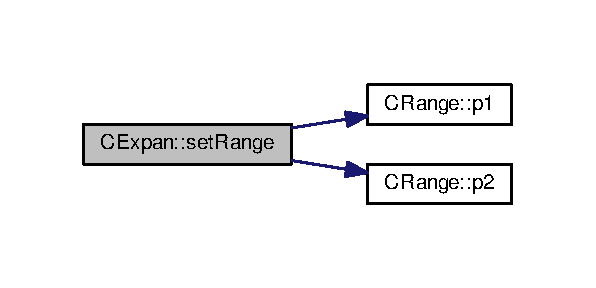
\includegraphics[width=286pt]{classCExpan_aa4ce064fc22518c150cabbbe15bba67f_cgraph}
\end{center}
\end{figure}


\hypertarget{classCExpan_ac044e829b5ac153720826b7d29c32afd}{\index{C\-Expan@{C\-Expan}!set\-Range@{set\-Range}}
\index{set\-Range@{set\-Range}!CExpan@{C\-Expan}}
\subsubsection[{set\-Range}]{\setlength{\rightskip}{0pt plus 5cm}void C\-Expan\-::set\-Range (
\begin{DoxyParamCaption}
\item[{int}]{p}
\end{DoxyParamCaption}
)\hspace{0.3cm}{\ttfamily [inline]}}}\label{classCExpan_ac044e829b5ac153720826b7d29c32afd}


Here is the call graph for this function\-:\nopagebreak
\begin{figure}[H]
\begin{center}
\leavevmode
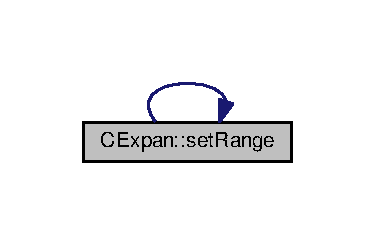
\includegraphics[width=180pt]{classCExpan_ac044e829b5ac153720826b7d29c32afd_cgraph}
\end{center}
\end{figure}


\hypertarget{classCExpan_aa36e147d92fd44b430f8962b2f358e8d}{\index{C\-Expan@{C\-Expan}!set\-Scale@{set\-Scale}}
\index{set\-Scale@{set\-Scale}!CExpan@{C\-Expan}}
\subsubsection[{set\-Scale}]{\setlength{\rightskip}{0pt plus 5cm}void C\-Expan\-::set\-Scale (
\begin{DoxyParamCaption}
\item[{double}]{scale}
\end{DoxyParamCaption}
)\hspace{0.3cm}{\ttfamily [inline]}}}\label{classCExpan_aa36e147d92fd44b430f8962b2f358e8d}
\hypertarget{classCExpan_ab384e5b3d427707106d655d8d9585ecc}{\index{C\-Expan@{C\-Expan}!set\-Vector@{set\-Vector}}
\index{set\-Vector@{set\-Vector}!CExpan@{C\-Expan}}
\subsubsection[{set\-Vector}]{\setlength{\rightskip}{0pt plus 5cm}void C\-Expan\-::set\-Vector (
\begin{DoxyParamCaption}
\item[{const {\bf R\-E\-A\-L} $\ast$}]{M, }
\item[{int}]{len}
\end{DoxyParamCaption}
)\hspace{0.3cm}{\ttfamily [inline]}}}\label{classCExpan_ab384e5b3d427707106d655d8d9585ecc}
\hypertarget{classCExpan_a61536819576535d2eb64f977b28134a0}{\index{C\-Expan@{C\-Expan}!undo@{undo}}
\index{undo@{undo}!CExpan@{C\-Expan}}
\subsubsection[{undo}]{\setlength{\rightskip}{0pt plus 5cm}void C\-Expan\-::undo (
\begin{DoxyParamCaption}
{}
\end{DoxyParamCaption}
)\hspace{0.3cm}{\ttfamily [inline]}}}\label{classCExpan_a61536819576535d2eb64f977b28134a0}


\subsection{Friends And Related Function Documentation}
\hypertarget{classCExpan_a5b8852acff77a8c6c5a167d050c7cee2}{\index{C\-Expan@{C\-Expan}!inprod\-\_\-unit\-Scale@{inprod\-\_\-unit\-Scale}}
\index{inprod\-\_\-unit\-Scale@{inprod\-\_\-unit\-Scale}!CExpan@{C\-Expan}}
\subsubsection[{inprod\-\_\-unit\-Scale}]{\setlength{\rightskip}{0pt plus 5cm}{\bf R\-E\-A\-L} inprod\-\_\-unit\-Scale (
\begin{DoxyParamCaption}
\item[{const {\bf C\-Expan} \&}]{E1, }
\item[{const {\bf C\-Expan} \&}]{E2}
\end{DoxyParamCaption}
)\hspace{0.3cm}{\ttfamily [friend]}}}\label{classCExpan_a5b8852acff77a8c6c5a167d050c7cee2}
\hypertarget{classCExpan_a35fefc436ee691468cdc7390ec783400}{\index{C\-Expan@{C\-Expan}!Is\-Scale\-Equal@{Is\-Scale\-Equal}}
\index{Is\-Scale\-Equal@{Is\-Scale\-Equal}!CExpan@{C\-Expan}}
\subsubsection[{Is\-Scale\-Equal}]{\setlength{\rightskip}{0pt plus 5cm}bool Is\-Scale\-Equal (
\begin{DoxyParamCaption}
\item[{const {\bf C\-Expan} \&}]{M1, }
\item[{const {\bf C\-Expan} \&}]{M2}
\end{DoxyParamCaption}
)\hspace{0.3cm}{\ttfamily [friend]}}}\label{classCExpan_a35fefc436ee691468cdc7390ec783400}
\hypertarget{classCExpan_a0dfbb05f2e29baa6aa8c097598bf9d45}{\index{C\-Expan@{C\-Expan}!operator$\ast$@{operator$\ast$}}
\index{operator$\ast$@{operator$\ast$}!CExpan@{C\-Expan}}
\subsubsection[{operator$\ast$}]{\setlength{\rightskip}{0pt plus 5cm}double operator$\ast$ (
\begin{DoxyParamCaption}
\item[{const {\bf C\-Expan} \&}]{E1, }
\item[{const {\bf C\-Expan} \&}]{E2}
\end{DoxyParamCaption}
)\hspace{0.3cm}{\ttfamily [friend]}}}\label{classCExpan_a0dfbb05f2e29baa6aa8c097598bf9d45}
\hypertarget{classCExpan_a70abf8064fc2c038c82602327d23da1a}{\index{C\-Expan@{C\-Expan}!operator$\ast$@{operator$\ast$}}
\index{operator$\ast$@{operator$\ast$}!CExpan@{C\-Expan}}
\subsubsection[{operator$\ast$}]{\setlength{\rightskip}{0pt plus 5cm}{\bf C\-Expan} operator$\ast$ (
\begin{DoxyParamCaption}
\item[{const {\bf C\-Expan} \&}]{E, }
\item[{const {\bf R\-E\-A\-L} $\ast$}]{C}
\end{DoxyParamCaption}
)\hspace{0.3cm}{\ttfamily [friend]}}}\label{classCExpan_a70abf8064fc2c038c82602327d23da1a}
\hypertarget{classCExpan_ac0b2a0b0ce2280f60412bb96aed5f3dd}{\index{C\-Expan@{C\-Expan}!operator$\ast$@{operator$\ast$}}
\index{operator$\ast$@{operator$\ast$}!CExpan@{C\-Expan}}
\subsubsection[{operator$\ast$}]{\setlength{\rightskip}{0pt plus 5cm}{\bf C\-Expan} operator$\ast$ (
\begin{DoxyParamCaption}
\item[{{\bf R\-E\-A\-L}}]{s, }
\item[{const {\bf C\-Expan} \&}]{E}
\end{DoxyParamCaption}
)\hspace{0.3cm}{\ttfamily [friend]}}}\label{classCExpan_ac0b2a0b0ce2280f60412bb96aed5f3dd}
\hypertarget{classCExpan_af86f70797548daca1b4c94f306eb22c3}{\index{C\-Expan@{C\-Expan}!operator+@{operator+}}
\index{operator+@{operator+}!CExpan@{C\-Expan}}
\subsubsection[{operator+}]{\setlength{\rightskip}{0pt plus 5cm}{\bf C\-Expan} operator+ (
\begin{DoxyParamCaption}
\item[{const {\bf C\-Expan} \&}]{E1, }
\item[{const {\bf C\-Expan} \&}]{E2}
\end{DoxyParamCaption}
)\hspace{0.3cm}{\ttfamily [friend]}}}\label{classCExpan_af86f70797548daca1b4c94f306eb22c3}
\hypertarget{classCExpan_a61b8986661aaa2d6f0eff5e5f2c58488}{\index{C\-Expan@{C\-Expan}!operator-\/@{operator-\/}}
\index{operator-\/@{operator-\/}!CExpan@{C\-Expan}}
\subsubsection[{operator-\/}]{\setlength{\rightskip}{0pt plus 5cm}{\bf C\-Expan} operator-\/ (
\begin{DoxyParamCaption}
\item[{const {\bf C\-Expan} \&}]{E1, }
\item[{const {\bf C\-Expan} \&}]{E2}
\end{DoxyParamCaption}
)\hspace{0.3cm}{\ttfamily [friend]}}}\label{classCExpan_a61b8986661aaa2d6f0eff5e5f2c58488}
\hypertarget{classCExpan_adfca34b8a78f7e0647ee4113707047c4}{\index{C\-Expan@{C\-Expan}!operator$<$$<$@{operator$<$$<$}}
\index{operator$<$$<$@{operator$<$$<$}!CExpan@{C\-Expan}}
\subsubsection[{operator$<$$<$}]{\setlength{\rightskip}{0pt plus 5cm}ostream\& operator$<$$<$ (
\begin{DoxyParamCaption}
\item[{ostream \&}]{out, }
\item[{const {\bf C\-Expan} \&}]{p}
\end{DoxyParamCaption}
)\hspace{0.3cm}{\ttfamily [friend]}}}\label{classCExpan_adfca34b8a78f7e0647ee4113707047c4}
Output the multipole expansion to a file 

\subsection{Member Data Documentation}
\hypertarget{classCExpan_a0e7564a3c13370795a342ce9d4b263a7}{\index{C\-Expan@{C\-Expan}!I\-D\-X@{I\-D\-X}}
\index{I\-D\-X@{I\-D\-X}!CExpan@{C\-Expan}}
\subsubsection[{I\-D\-X}]{\setlength{\rightskip}{0pt plus 5cm}int C\-Expan\-::\-I\-D\-X\hspace{0.3cm}{\ttfamily [static]}}}\label{classCExpan_a0e7564a3c13370795a342ce9d4b263a7}


Contains the index for first position of constants of every n level. 

\hypertarget{classCExpan_a4b0d1b36d98257b16600f1ffc6d20ba3}{\index{C\-Expan@{C\-Expan}!I\-S\-Q\-R\-T2@{I\-S\-Q\-R\-T2}}
\index{I\-S\-Q\-R\-T2@{I\-S\-Q\-R\-T2}!CExpan@{C\-Expan}}
\subsubsection[{I\-S\-Q\-R\-T2}]{\setlength{\rightskip}{0pt plus 5cm}{\bf R\-E\-A\-L} C\-Expan\-::\-I\-S\-Q\-R\-T2 = sqrt( 1.\-0 )\hspace{0.3cm}{\ttfamily [static]}}}\label{classCExpan_a4b0d1b36d98257b16600f1ffc6d20ba3}
\hypertarget{classCExpan_a6016c7f7b961e2f69c6d7ca9daedbbf5}{\index{C\-Expan@{C\-Expan}!m\-\_\-\-M@{m\-\_\-\-M}}
\index{m\-\_\-\-M@{m\-\_\-\-M}!CExpan@{C\-Expan}}
\subsubsection[{m\-\_\-\-M}]{\setlength{\rightskip}{0pt plus 5cm}vector$<${\bf R\-E\-A\-L}$>$ C\-Expan\-::m\-\_\-\-M\hspace{0.3cm}{\ttfamily [protected]}}}\label{classCExpan_a6016c7f7b961e2f69c6d7ca9daedbbf5}
\hypertarget{classCExpan_a151aff07c3667229bfa6d9d3e6e87dfc}{\index{C\-Expan@{C\-Expan}!m\-\_\-\-M\-U@{m\-\_\-\-M\-U}}
\index{m\-\_\-\-M\-U@{m\-\_\-\-M\-U}!CExpan@{C\-Expan}}
\subsubsection[{m\-\_\-\-M\-U}]{\setlength{\rightskip}{0pt plus 5cm}vector$<${\bf R\-E\-A\-L}$>$ C\-Expan\-::m\-\_\-\-M\-U\hspace{0.3cm}{\ttfamily [protected]}}}\label{classCExpan_a151aff07c3667229bfa6d9d3e6e87dfc}
\hypertarget{classCExpan_adca887f9cd66e5e5c800a41c3e406559}{\index{C\-Expan@{C\-Expan}!m\-\_\-range@{m\-\_\-range}}
\index{m\-\_\-range@{m\-\_\-range}!CExpan@{C\-Expan}}
\subsubsection[{m\-\_\-range}]{\setlength{\rightskip}{0pt plus 5cm}{\bf C\-Range} C\-Expan\-::m\-\_\-range\hspace{0.3cm}{\ttfamily [protected]}}}\label{classCExpan_adca887f9cd66e5e5c800a41c3e406559}


A range object of current expansion. 

\hypertarget{classCExpan_ae9c36d68e7ef5bdf74ad220141367792}{\index{C\-Expan@{C\-Expan}!m\-\_\-range\-U@{m\-\_\-range\-U}}
\index{m\-\_\-range\-U@{m\-\_\-range\-U}!CExpan@{C\-Expan}}
\subsubsection[{m\-\_\-range\-U}]{\setlength{\rightskip}{0pt plus 5cm}{\bf C\-Range} C\-Expan\-::m\-\_\-range\-U\hspace{0.3cm}{\ttfamily [protected]}}}\label{classCExpan_ae9c36d68e7ef5bdf74ad220141367792}


A saved range object of previous expansion, stored for undo. 

\hypertarget{classCExpan_a4dba59941eefe0f6d70fb89f1e610d77}{\index{C\-Expan@{C\-Expan}!m\-\_\-scale@{m\-\_\-scale}}
\index{m\-\_\-scale@{m\-\_\-scale}!CExpan@{C\-Expan}}
\subsubsection[{m\-\_\-scale}]{\setlength{\rightskip}{0pt plus 5cm}double C\-Expan\-::m\-\_\-scale\hspace{0.3cm}{\ttfamily [protected]}}}\label{classCExpan_a4dba59941eefe0f6d70fb89f1e610d77}
\hypertarget{classCExpan_a16aade514bb13da387040369e7137aeb}{\index{C\-Expan@{C\-Expan}!m\-\_\-scale\-U@{m\-\_\-scale\-U}}
\index{m\-\_\-scale\-U@{m\-\_\-scale\-U}!CExpan@{C\-Expan}}
\subsubsection[{m\-\_\-scale\-U}]{\setlength{\rightskip}{0pt plus 5cm}double C\-Expan\-::m\-\_\-scale\-U\hspace{0.3cm}{\ttfamily [protected]}}}\label{classCExpan_a16aade514bb13da387040369e7137aeb}
\hypertarget{classCExpan_a1e3c0894a6550c4b01722e9741c83666}{\index{C\-Expan@{C\-Expan}!R\-A\-T\-I\-O@{R\-A\-T\-I\-O}}
\index{R\-A\-T\-I\-O@{R\-A\-T\-I\-O}!CExpan@{C\-Expan}}
\subsubsection[{R\-A\-T\-I\-O}]{\setlength{\rightskip}{0pt plus 5cm}{\bf R\-E\-A\-L} C\-Expan\-::\-R\-A\-T\-I\-O = 18.\-0\hspace{0.3cm}{\ttfamily [static]}, {\ttfamily [protected]}}}\label{classCExpan_a1e3c0894a6550c4b01722e9741c83666}
\hypertarget{classCExpan_aa5282327718d2c6dbff1ef2fbc0fe4dd}{\index{C\-Expan@{C\-Expan}!S\-Q\-R\-T2@{S\-Q\-R\-T2}}
\index{S\-Q\-R\-T2@{S\-Q\-R\-T2}!CExpan@{C\-Expan}}
\subsubsection[{S\-Q\-R\-T2}]{\setlength{\rightskip}{0pt plus 5cm}{\bf R\-E\-A\-L} C\-Expan\-::\-S\-Q\-R\-T2 = sqrt( 1.\-0 )\hspace{0.3cm}{\ttfamily [static]}}}\label{classCExpan_aa5282327718d2c6dbff1ef2fbc0fe4dd}


The documentation for this class was generated from the following files\-:\begin{DoxyCompactItemize}
\item 
\hyperlink{expansion_8h}{expansion.\-h}\item 
\hyperlink{expansion_8cpp}{expansion.\-cpp}\end{DoxyCompactItemize}

\hypertarget{classCExpCenter}{\section{C\-Exp\-Center Class Reference}
\label{classCExpCenter}\index{C\-Exp\-Center@{C\-Exp\-Center}}
}


\hyperlink{classCExpCenter}{C\-Exp\-Center} class.  




{\ttfamily \#include $<$expcenter.\-h$>$}



Inheritance diagram for C\-Exp\-Center\-:\nopagebreak
\begin{figure}[H]
\begin{center}
\leavevmode
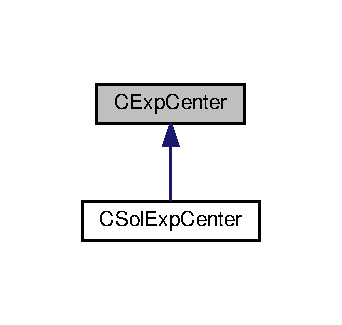
\includegraphics[width=164pt]{classCExpCenter__inherit__graph}
\end{center}
\end{figure}


Collaboration diagram for C\-Exp\-Center\-:\nopagebreak
\begin{figure}[H]
\begin{center}
\leavevmode
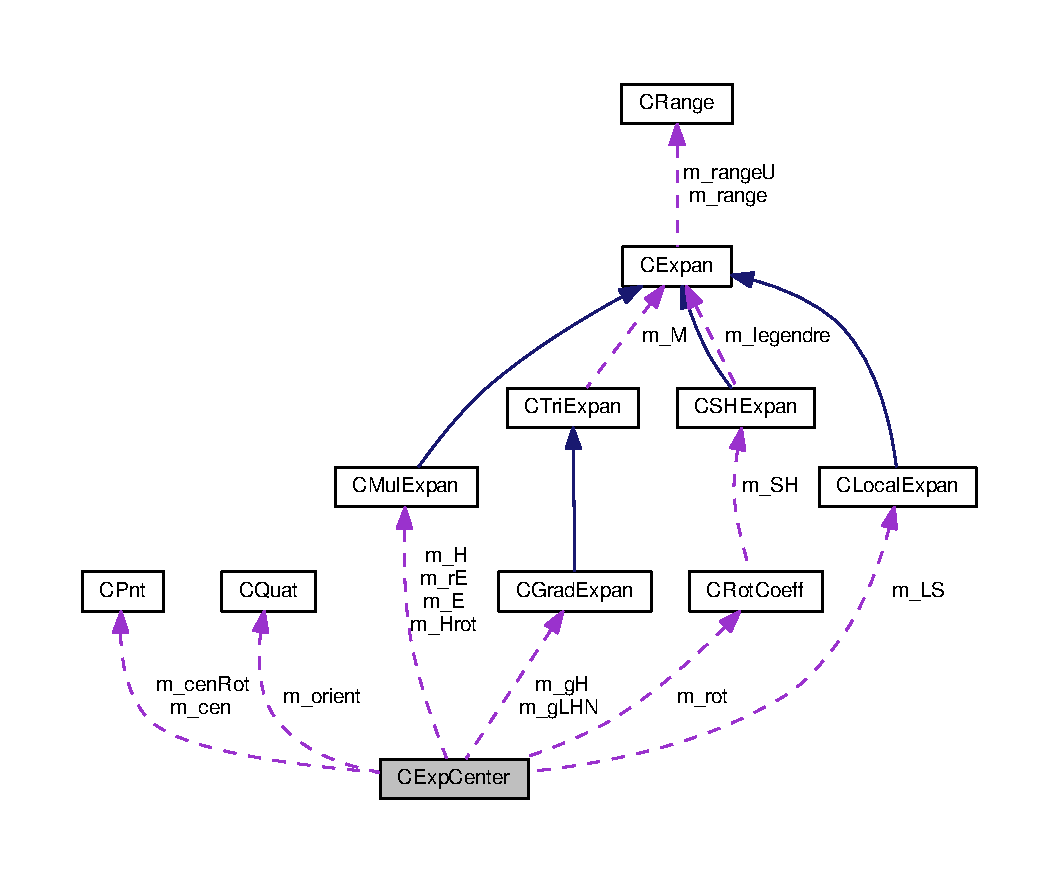
\includegraphics[width=350pt]{classCExpCenter__coll__graph}
\end{center}
\end{figure}
\subsection*{Public Member Functions}
\begin{DoxyCompactItemize}
\item 
\hyperlink{classCExpCenter_abd3f14d423a6a1f8404380edb34f8d7c}{C\-Exp\-Center} ()
\item 
\hyperlink{classCExpCenter_a91bbc8f8561e58eeab18595df4f320b4}{C\-Exp\-Center} (int ki, \hyperlink{classCPnt}{C\-Pnt} cen, double rad)
\item 
\hyperlink{classCExpCenter_a8272991c2429ea236f18b2ae4fe33546}{C\-Exp\-Center} (int ki, \hyperlink{classCPnt}{C\-Pnt} cen, double rad, double idiel, bool b\-Kappa, const vector$<$ double $>$ \&chg\-Assigned, const vector$<$ \hyperlink{classCPnt}{C\-Pnt} $>$ \&pos\-Assigned, \hyperlink{classCQuat}{C\-Quat} $\ast$orient=N\-U\-L\-L, \hyperlink{classCRotCoeff}{C\-Rot\-Coeff} $\ast$rot=N\-U\-L\-L)
\item 
void \hyperlink{classCExpCenter_a6d4be76f4a28b68eca9dcd4a778ca387}{set\-Order} (const int p, const \hyperlink{classCRotCoeff}{C\-Rot\-Coeff} \&rot)
\item 
void \hyperlink{classCExpCenter_a91e9e5e3ffbf36281c1b7da46aa12c75}{inc\-Order} (const \hyperlink{classCRotCoeff}{C\-Rot\-Coeff} \&rot)
\item 
const \hyperlink{util_8h_a5821460e95a0800cf9f24c38915cbbde}{R\-E\-A\-L} \hyperlink{classCExpCenter_adff5ce73777a1d3045f0609dd0e955cf}{compute\-Pot} () const 
\item 
const double \hyperlink{classCExpCenter_adc18426f677b5984a468101ebfeefef6}{get\-Rad} () const 
\item 
const \hyperlink{classCPnt}{C\-Pnt} \hyperlink{classCExpCenter_a84f867868f8eb0785e95561f26cd0194}{get\-Cen} () const 
\item 
const \hyperlink{classCPnt}{C\-Pnt} \hyperlink{classCExpCenter_a69ce8d87ba63324aa16349019e6b71d4}{get\-Cen\-Rot} () const 
\item 
const \hyperlink{classCQuat}{C\-Quat} \hyperlink{classCExpCenter_a069965ee754068a0f59e3b80dbb8252c}{get\-Orient} () const 
\item 
const int \hyperlink{classCExpCenter_a18e5340638fc144dfa255cef7d5214d9}{get\-Order} () const 
\item 
const double \hyperlink{classCExpCenter_a30c3a26e0dc5bc9c2d84d366200243e5}{get\-L\-Scale} () const 
\item 
const double \hyperlink{classCExpCenter_ab58aa40813bf06929764f6b9ae4a25d1}{get\-M\-Scale} () const 
\item 
const bool \hyperlink{classCExpCenter_aac86d77bd8353ccf10bb6b8f229575c7}{getb\-Kappa} () const 
\item 
const \hyperlink{classCMulExpan}{C\-Mul\-Expan} $\ast$const \hyperlink{classCExpCenter_a6f8eb6dfa6331e8d75a04ec7998a603c}{getp\-H} () const 
\item 
\hyperlink{classCMulExpan}{C\-Mul\-Expan} $\ast$const \hyperlink{classCExpCenter_a6a9a76aa4ddcbb79a4cee534f7c48d07}{getp\-H} ()
\item 
\hyperlink{classCMulExpan}{C\-Mul\-Expan} \& \hyperlink{classCExpCenter_a2051390bfbef8a9fd1e045cab42b99ba}{get\-H} ()
\item 
const \hyperlink{classCMulExpan}{C\-Mul\-Expan} \hyperlink{classCExpCenter_ad4efe45a4f948726fcfcecb975d5044d}{get\-H} () const 
\item 
\hyperlink{classCMulExpan}{C\-Mul\-Expan} \& \hyperlink{classCExpCenter_aff64017f498b93ed212c674865f95f40}{get\-Hrot} ()
\item 
const \hyperlink{classCMulExpan}{C\-Mul\-Expan} \hyperlink{classCExpCenter_aff23edad5050d0e1b80e72a90d1fbb7a}{get\-Hrot} () const 
\item 
const double \hyperlink{classCExpCenter_a1206c32b0699ae5eef35dd1f88cf9816}{get\-Hrot\-Mono} () const 
\item 
\hyperlink{classCLocalExpan}{C\-Local\-Expan} \& \hyperlink{classCExpCenter_aba7d7d3c0f0b49e28d66f96621be677e}{get\-L\-S} ()
\item 
const \hyperlink{classCLocalExpan}{C\-Local\-Expan} \& \hyperlink{classCExpCenter_a7269ed18262fdfff4d066fbe8521b928}{get\-L\-S} () const 
\item 
const \hyperlink{classCMulExpan}{C\-Mul\-Expan} \hyperlink{classCExpCenter_a1e57fde5e2b0b605633dd57a083347bd}{getr\-E} () const 
\item 
\hyperlink{classCGradExpan}{C\-Grad\-Expan} \& \hyperlink{classCExpCenter_a070d0724a38ffb86095a95eacb55aac1}{getg\-L\-H\-N} ()
\item 
const \hyperlink{classCGradExpan}{C\-Grad\-Expan} \hyperlink{classCExpCenter_a94e7b22b07e8224827c489e84d26e155}{getg\-L\-H\-N} () const 
\item 
\hyperlink{classCExpCenter}{C\-Exp\-Center} \& \hyperlink{classCExpCenter_a169ca7822910b6a9906b1d6050278af8}{operator=} (const \hyperlink{classCExpCenter}{C\-Exp\-Center} \&M)
\item 
const \hyperlink{classCRotCoeff}{C\-Rot\-Coeff} \hyperlink{classCExpCenter_a74d5d90cdcf9b6a61540b607b0269a23}{get\-Rot\-Coeff} () const 
\end{DoxyCompactItemize}
\subsection*{Static Public Member Functions}
\begin{DoxyCompactItemize}
\item 
static void \hyperlink{classCExpCenter_a4b8dab75eef2c0fee471f844a55d1af3}{init\-Constants} (double sdiel, double kappa)
\begin{DoxyCompactList}\small\item\em \hyperlink{classCExpCenter}{C\-Exp\-Center} init\-Constants function. \end{DoxyCompactList}\end{DoxyCompactItemize}
\subsection*{Protected Member Functions}
\begin{DoxyCompactItemize}
\item 
void \hyperlink{classCExpCenter_a44ea6f7aa0c0c37c721ed35e0b702703}{set\-Fixed\-Charges} ()
\end{DoxyCompactItemize}
\subsection*{Protected Attributes}
\begin{DoxyCompactItemize}
\item 
\hyperlink{classCPnt}{C\-Pnt} \hyperlink{classCExpCenter_a57a81c26f40939d189a88b82c77f16e8}{m\-\_\-cen}
\begin{DoxyCompactList}\small\item\em An xyz of the center of the molecule in the standard frame. \end{DoxyCompactList}\item 
\hyperlink{classCPnt}{C\-Pnt} \hyperlink{classCExpCenter_a73b0d497d54258b3ab503167ae6f7e75}{m\-\_\-cen\-Rot}
\item 
double \hyperlink{classCExpCenter_abc237f77679da4a21619a384e6ff4f6b}{m\-\_\-rad}
\begin{DoxyCompactList}\small\item\em A floating point of the current C\-G sphere's radius (a$^\wedge$(I,k)) \end{DoxyCompactList}\item 
double \hyperlink{classCExpCenter_aac9d9de905652a9d78115a1b53091bce}{m\-\_\-lscale}
\begin{DoxyCompactList}\small\item\em A floating point of the length scale of the current sphere, defaulted to m\-\_\-rad. \end{DoxyCompactList}\item 
double \hyperlink{classCExpCenter_a7182695f02cc43411ebc67e64258a2ec}{m\-\_\-mscale}
\begin{DoxyCompactList}\small\item\em A floating point of another length scale, defaulted to 1/m\-\_\-rad. \end{DoxyCompactList}\item 
double \hyperlink{classCExpCenter_a2ebe2d840aaaa9329706514fa6957efa}{m\-\_\-idiel}
\begin{DoxyCompactList}\small\item\em A floating point of the molecule's interior dielectric constant. \end{DoxyCompactList}\item 
bool \hyperlink{classCExpCenter_a9012e39bbe103cd93190156817b0efb4}{m\-\_\-b\-Kappa}
\item 
vector$<$ double $>$ \hyperlink{classCExpCenter_a834cd8238e3d5fd2b29a487d08f93978}{m\-\_\-ch}
\item 
vector$<$ \hyperlink{classCPnt}{C\-Pnt} $>$ \hyperlink{classCExpCenter_a6d2bc11475081445ad8838d6deb889d3}{m\-\_\-pos}
\item 
\hyperlink{classCLocalExpan}{C\-Local\-Expan} \hyperlink{classCExpCenter_a89612776d4a057bdd4d36a7b4e10e647}{m\-\_\-\-L\-S}
\begin{DoxyCompactList}\small\item\em only due to external source ( selected ) \end{DoxyCompactList}\item 
\hyperlink{classCMulExpan}{C\-Mul\-Expan} \hyperlink{classCExpCenter_a41728832a9a82eec510548f438e65734}{m\-\_\-\-E}
\item 
\hyperlink{classCMulExpan}{C\-Mul\-Expan} \hyperlink{classCExpCenter_a4c494c322b3272097b3b6aadfc2959f6}{m\-\_\-r\-E}
\item 
\hyperlink{classCMulExpan}{C\-Mul\-Expan} \hyperlink{classCExpCenter_a6cf480aad64c9baf8a126d308ca63f85}{m\-\_\-\-H}
\begin{DoxyCompactList}\small\item\em A multipole expansion of the effective polarization charges on sphere k of the exposed surf. \end{DoxyCompactList}\item 
\hyperlink{classCMulExpan}{C\-Mul\-Expan} \hyperlink{classCExpCenter_acfe6c4c74d9fd3069d00fef085eafbd8}{m\-\_\-\-Hrot}
\begin{DoxyCompactList}\small\item\em A rotated M\-P\-E of the effective polarization charges on sphere k of the exposed surf. \end{DoxyCompactList}\item 
\hyperlink{classCGradExpan}{C\-Grad\-Expan} \hyperlink{classCExpCenter_ae860d91bb83f5b31eff56694f6428e20}{m\-\_\-g\-H}
\item 
\hyperlink{classCGradExpan}{C\-Grad\-Expan} \hyperlink{classCExpCenter_a2ac196fbf3b2a5623553b4ecdc30cd7f}{m\-\_\-g\-L\-H\-N}
\item 
\hyperlink{classCQuat}{C\-Quat} $\ast$ \hyperlink{classCExpCenter_a49742562fd68129ab17aa716e6e661e8}{m\-\_\-orient}
\begin{DoxyCompactList}\small\item\em A quaterion of the the current rotation of the molecule. \end{DoxyCompactList}\item 
\hyperlink{classCRotCoeff}{C\-Rot\-Coeff} $\ast$ \hyperlink{classCExpCenter_a284a13e418738579f101ad9dc0af4dec}{m\-\_\-rot}
\item 
int \hyperlink{classCExpCenter_a2a3e3bc7c527c49e9ea4149dd33f4dba}{m\-\_\-p}
\begin{DoxyCompactList}\small\item\em An integer of the number of poles in the expansion. \end{DoxyCompactList}\item 
int \hyperlink{classCExpCenter_a7dcda3540f2ff0b3bfd668889ef1e95a}{m\-\_\-id}
\begin{DoxyCompactList}\small\item\em An integer of the I\-D number of the C\-G sphere. \end{DoxyCompactList}\end{DoxyCompactItemize}
\subsection*{Static Protected Attributes}
\begin{DoxyCompactItemize}
\item 
static double \hyperlink{classCExpCenter_a027b6ddd209098aa7f6c71f7b43367b3}{m\-\_\-sdiel}
\begin{DoxyCompactList}\small\item\em A floating point of the solvent dielectric constant. \end{DoxyCompactList}\item 
static double \hyperlink{classCExpCenter_aca58b7a93949d83d4b7883b54d0473e5}{m\-\_\-kappa}
\begin{DoxyCompactList}\small\item\em A floating point of the system's inverse debye length. \end{DoxyCompactList}\end{DoxyCompactItemize}


\subsection{Detailed Description}
\hyperlink{classCExpCenter}{C\-Exp\-Center} class. 

This class is the base class for all expansion centers 

\subsection{Constructor \& Destructor Documentation}
\hypertarget{classCExpCenter_abd3f14d423a6a1f8404380edb34f8d7c}{\index{C\-Exp\-Center@{C\-Exp\-Center}!C\-Exp\-Center@{C\-Exp\-Center}}
\index{C\-Exp\-Center@{C\-Exp\-Center}!CExpCenter@{C\-Exp\-Center}}
\subsubsection[{C\-Exp\-Center}]{\setlength{\rightskip}{0pt plus 5cm}C\-Exp\-Center\-::\-C\-Exp\-Center (
\begin{DoxyParamCaption}
{}
\end{DoxyParamCaption}
)}}\label{classCExpCenter_abd3f14d423a6a1f8404380edb34f8d7c}
Constructor for Exp\-Center class \hypertarget{classCExpCenter_a91bbc8f8561e58eeab18595df4f320b4}{\index{C\-Exp\-Center@{C\-Exp\-Center}!C\-Exp\-Center@{C\-Exp\-Center}}
\index{C\-Exp\-Center@{C\-Exp\-Center}!CExpCenter@{C\-Exp\-Center}}
\subsubsection[{C\-Exp\-Center}]{\setlength{\rightskip}{0pt plus 5cm}C\-Exp\-Center\-::\-C\-Exp\-Center (
\begin{DoxyParamCaption}
\item[{int}]{ki, }
\item[{{\bf C\-Pnt}}]{cen, }
\item[{double}]{rad}
\end{DoxyParamCaption}
)}}\label{classCExpCenter_a91bbc8f8561e58eeab18595df4f320b4}
Constructor for Exp\-Center class \hypertarget{classCExpCenter_a8272991c2429ea236f18b2ae4fe33546}{\index{C\-Exp\-Center@{C\-Exp\-Center}!C\-Exp\-Center@{C\-Exp\-Center}}
\index{C\-Exp\-Center@{C\-Exp\-Center}!CExpCenter@{C\-Exp\-Center}}
\subsubsection[{C\-Exp\-Center}]{\setlength{\rightskip}{0pt plus 5cm}C\-Exp\-Center\-::\-C\-Exp\-Center (
\begin{DoxyParamCaption}
\item[{int}]{ki, }
\item[{{\bf C\-Pnt}}]{cen, }
\item[{double}]{rad, }
\item[{double}]{idiel, }
\item[{bool}]{b\-Kappa, }
\item[{const vector$<$ double $>$ \&}]{chg\-Assigned, }
\item[{const vector$<$ {\bf C\-Pnt} $>$ \&}]{pos\-Assigned, }
\item[{{\bf C\-Quat} $\ast$}]{orient = {\ttfamily NULL}, }
\item[{{\bf C\-Rot\-Coeff} $\ast$}]{rot = {\ttfamily NULL}}
\end{DoxyParamCaption}
)}}\label{classCExpCenter_a8272991c2429ea236f18b2ae4fe33546}
Constructor for Exp\-Center class 

Here is the call graph for this function\-:\nopagebreak
\begin{figure}[H]
\begin{center}
\leavevmode
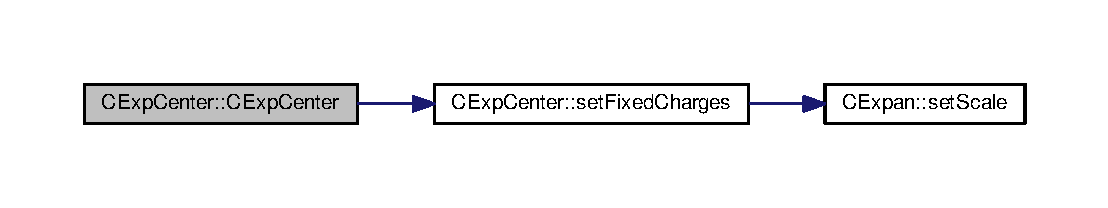
\includegraphics[width=350pt]{classCExpCenter_a8272991c2429ea236f18b2ae4fe33546_cgraph}
\end{center}
\end{figure}




\subsection{Member Function Documentation}
\hypertarget{classCExpCenter_adff5ce73777a1d3045f0609dd0e955cf}{\index{C\-Exp\-Center@{C\-Exp\-Center}!compute\-Pot@{compute\-Pot}}
\index{compute\-Pot@{compute\-Pot}!CExpCenter@{C\-Exp\-Center}}
\subsubsection[{compute\-Pot}]{\setlength{\rightskip}{0pt plus 5cm}const {\bf R\-E\-A\-L} C\-Exp\-Center\-::compute\-Pot (
\begin{DoxyParamCaption}
{}
\end{DoxyParamCaption}
) const}}\label{classCExpCenter_adff5ce73777a1d3045f0609dd0e955cf}
Computes interaction energy of center with ext potential 

Here is the call graph for this function\-:\nopagebreak
\begin{figure}[H]
\begin{center}
\leavevmode
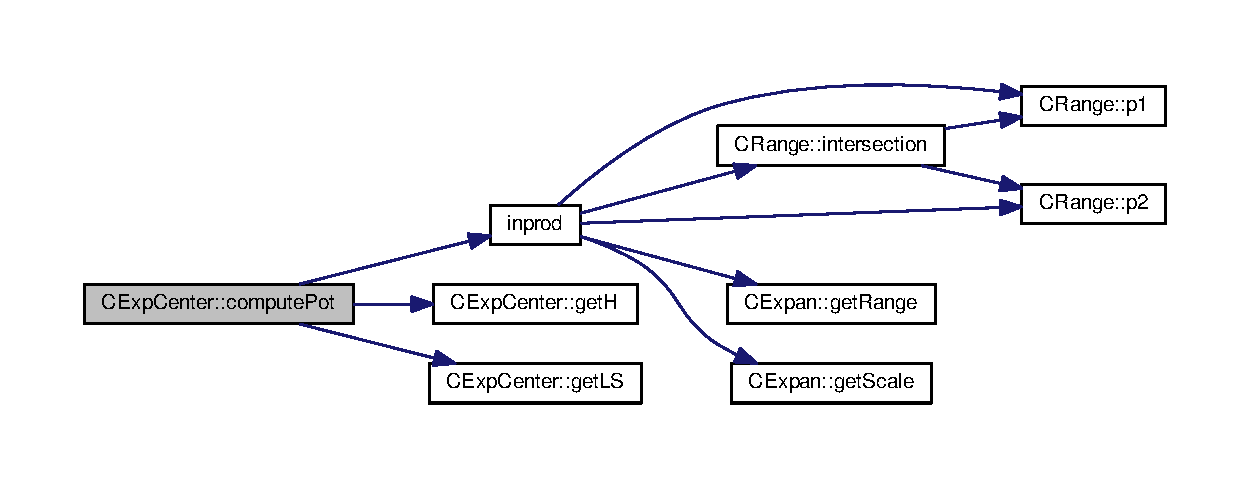
\includegraphics[width=350pt]{classCExpCenter_adff5ce73777a1d3045f0609dd0e955cf_cgraph}
\end{center}
\end{figure}


\hypertarget{classCExpCenter_aac86d77bd8353ccf10bb6b8f229575c7}{\index{C\-Exp\-Center@{C\-Exp\-Center}!getb\-Kappa@{getb\-Kappa}}
\index{getb\-Kappa@{getb\-Kappa}!CExpCenter@{C\-Exp\-Center}}
\subsubsection[{getb\-Kappa}]{\setlength{\rightskip}{0pt plus 5cm}const bool C\-Exp\-Center\-::getb\-Kappa (
\begin{DoxyParamCaption}
{}
\end{DoxyParamCaption}
) const\hspace{0.3cm}{\ttfamily [inline]}}}\label{classCExpCenter_aac86d77bd8353ccf10bb6b8f229575c7}
\hypertarget{classCExpCenter_a84f867868f8eb0785e95561f26cd0194}{\index{C\-Exp\-Center@{C\-Exp\-Center}!get\-Cen@{get\-Cen}}
\index{get\-Cen@{get\-Cen}!CExpCenter@{C\-Exp\-Center}}
\subsubsection[{get\-Cen}]{\setlength{\rightskip}{0pt plus 5cm}const {\bf C\-Pnt} C\-Exp\-Center\-::get\-Cen (
\begin{DoxyParamCaption}
{}
\end{DoxyParamCaption}
) const\hspace{0.3cm}{\ttfamily [inline]}}}\label{classCExpCenter_a84f867868f8eb0785e95561f26cd0194}
\hypertarget{classCExpCenter_a69ce8d87ba63324aa16349019e6b71d4}{\index{C\-Exp\-Center@{C\-Exp\-Center}!get\-Cen\-Rot@{get\-Cen\-Rot}}
\index{get\-Cen\-Rot@{get\-Cen\-Rot}!CExpCenter@{C\-Exp\-Center}}
\subsubsection[{get\-Cen\-Rot}]{\setlength{\rightskip}{0pt plus 5cm}const {\bf C\-Pnt} C\-Exp\-Center\-::get\-Cen\-Rot (
\begin{DoxyParamCaption}
{}
\end{DoxyParamCaption}
) const\hspace{0.3cm}{\ttfamily [inline]}}}\label{classCExpCenter_a69ce8d87ba63324aa16349019e6b71d4}
\hypertarget{classCExpCenter_a070d0724a38ffb86095a95eacb55aac1}{\index{C\-Exp\-Center@{C\-Exp\-Center}!getg\-L\-H\-N@{getg\-L\-H\-N}}
\index{getg\-L\-H\-N@{getg\-L\-H\-N}!CExpCenter@{C\-Exp\-Center}}
\subsubsection[{getg\-L\-H\-N}]{\setlength{\rightskip}{0pt plus 5cm}{\bf C\-Grad\-Expan}\& C\-Exp\-Center\-::getg\-L\-H\-N (
\begin{DoxyParamCaption}
{}
\end{DoxyParamCaption}
)\hspace{0.3cm}{\ttfamily [inline]}}}\label{classCExpCenter_a070d0724a38ffb86095a95eacb55aac1}
\hypertarget{classCExpCenter_a94e7b22b07e8224827c489e84d26e155}{\index{C\-Exp\-Center@{C\-Exp\-Center}!getg\-L\-H\-N@{getg\-L\-H\-N}}
\index{getg\-L\-H\-N@{getg\-L\-H\-N}!CExpCenter@{C\-Exp\-Center}}
\subsubsection[{getg\-L\-H\-N}]{\setlength{\rightskip}{0pt plus 5cm}const {\bf C\-Grad\-Expan} C\-Exp\-Center\-::getg\-L\-H\-N (
\begin{DoxyParamCaption}
{}
\end{DoxyParamCaption}
) const\hspace{0.3cm}{\ttfamily [inline]}}}\label{classCExpCenter_a94e7b22b07e8224827c489e84d26e155}
\hypertarget{classCExpCenter_a2051390bfbef8a9fd1e045cab42b99ba}{\index{C\-Exp\-Center@{C\-Exp\-Center}!get\-H@{get\-H}}
\index{get\-H@{get\-H}!CExpCenter@{C\-Exp\-Center}}
\subsubsection[{get\-H}]{\setlength{\rightskip}{0pt plus 5cm}{\bf C\-Mul\-Expan}\& C\-Exp\-Center\-::get\-H (
\begin{DoxyParamCaption}
{}
\end{DoxyParamCaption}
)\hspace{0.3cm}{\ttfamily [inline]}}}\label{classCExpCenter_a2051390bfbef8a9fd1e045cab42b99ba}
\hypertarget{classCExpCenter_ad4efe45a4f948726fcfcecb975d5044d}{\index{C\-Exp\-Center@{C\-Exp\-Center}!get\-H@{get\-H}}
\index{get\-H@{get\-H}!CExpCenter@{C\-Exp\-Center}}
\subsubsection[{get\-H}]{\setlength{\rightskip}{0pt plus 5cm}const {\bf C\-Mul\-Expan} C\-Exp\-Center\-::get\-H (
\begin{DoxyParamCaption}
{}
\end{DoxyParamCaption}
) const\hspace{0.3cm}{\ttfamily [inline]}}}\label{classCExpCenter_ad4efe45a4f948726fcfcecb975d5044d}
\hypertarget{classCExpCenter_aff64017f498b93ed212c674865f95f40}{\index{C\-Exp\-Center@{C\-Exp\-Center}!get\-Hrot@{get\-Hrot}}
\index{get\-Hrot@{get\-Hrot}!CExpCenter@{C\-Exp\-Center}}
\subsubsection[{get\-Hrot}]{\setlength{\rightskip}{0pt plus 5cm}{\bf C\-Mul\-Expan}\& C\-Exp\-Center\-::get\-Hrot (
\begin{DoxyParamCaption}
{}
\end{DoxyParamCaption}
)\hspace{0.3cm}{\ttfamily [inline]}}}\label{classCExpCenter_aff64017f498b93ed212c674865f95f40}
\hypertarget{classCExpCenter_aff23edad5050d0e1b80e72a90d1fbb7a}{\index{C\-Exp\-Center@{C\-Exp\-Center}!get\-Hrot@{get\-Hrot}}
\index{get\-Hrot@{get\-Hrot}!CExpCenter@{C\-Exp\-Center}}
\subsubsection[{get\-Hrot}]{\setlength{\rightskip}{0pt plus 5cm}const {\bf C\-Mul\-Expan} C\-Exp\-Center\-::get\-Hrot (
\begin{DoxyParamCaption}
{}
\end{DoxyParamCaption}
) const\hspace{0.3cm}{\ttfamily [inline]}}}\label{classCExpCenter_aff23edad5050d0e1b80e72a90d1fbb7a}
\hypertarget{classCExpCenter_a1206c32b0699ae5eef35dd1f88cf9816}{\index{C\-Exp\-Center@{C\-Exp\-Center}!get\-Hrot\-Mono@{get\-Hrot\-Mono}}
\index{get\-Hrot\-Mono@{get\-Hrot\-Mono}!CExpCenter@{C\-Exp\-Center}}
\subsubsection[{get\-Hrot\-Mono}]{\setlength{\rightskip}{0pt plus 5cm}const double C\-Exp\-Center\-::get\-Hrot\-Mono (
\begin{DoxyParamCaption}
{}
\end{DoxyParamCaption}
) const\hspace{0.3cm}{\ttfamily [inline]}}}\label{classCExpCenter_a1206c32b0699ae5eef35dd1f88cf9816}
\hypertarget{classCExpCenter_aba7d7d3c0f0b49e28d66f96621be677e}{\index{C\-Exp\-Center@{C\-Exp\-Center}!get\-L\-S@{get\-L\-S}}
\index{get\-L\-S@{get\-L\-S}!CExpCenter@{C\-Exp\-Center}}
\subsubsection[{get\-L\-S}]{\setlength{\rightskip}{0pt plus 5cm}{\bf C\-Local\-Expan}\& C\-Exp\-Center\-::get\-L\-S (
\begin{DoxyParamCaption}
{}
\end{DoxyParamCaption}
)\hspace{0.3cm}{\ttfamily [inline]}}}\label{classCExpCenter_aba7d7d3c0f0b49e28d66f96621be677e}
\hypertarget{classCExpCenter_a7269ed18262fdfff4d066fbe8521b928}{\index{C\-Exp\-Center@{C\-Exp\-Center}!get\-L\-S@{get\-L\-S}}
\index{get\-L\-S@{get\-L\-S}!CExpCenter@{C\-Exp\-Center}}
\subsubsection[{get\-L\-S}]{\setlength{\rightskip}{0pt plus 5cm}const {\bf C\-Local\-Expan}\& C\-Exp\-Center\-::get\-L\-S (
\begin{DoxyParamCaption}
{}
\end{DoxyParamCaption}
) const\hspace{0.3cm}{\ttfamily [inline]}}}\label{classCExpCenter_a7269ed18262fdfff4d066fbe8521b928}
\hypertarget{classCExpCenter_a30c3a26e0dc5bc9c2d84d366200243e5}{\index{C\-Exp\-Center@{C\-Exp\-Center}!get\-L\-Scale@{get\-L\-Scale}}
\index{get\-L\-Scale@{get\-L\-Scale}!CExpCenter@{C\-Exp\-Center}}
\subsubsection[{get\-L\-Scale}]{\setlength{\rightskip}{0pt plus 5cm}const double C\-Exp\-Center\-::get\-L\-Scale (
\begin{DoxyParamCaption}
{}
\end{DoxyParamCaption}
) const\hspace{0.3cm}{\ttfamily [inline]}}}\label{classCExpCenter_a30c3a26e0dc5bc9c2d84d366200243e5}
\hypertarget{classCExpCenter_ab58aa40813bf06929764f6b9ae4a25d1}{\index{C\-Exp\-Center@{C\-Exp\-Center}!get\-M\-Scale@{get\-M\-Scale}}
\index{get\-M\-Scale@{get\-M\-Scale}!CExpCenter@{C\-Exp\-Center}}
\subsubsection[{get\-M\-Scale}]{\setlength{\rightskip}{0pt plus 5cm}const double C\-Exp\-Center\-::get\-M\-Scale (
\begin{DoxyParamCaption}
{}
\end{DoxyParamCaption}
) const\hspace{0.3cm}{\ttfamily [inline]}}}\label{classCExpCenter_ab58aa40813bf06929764f6b9ae4a25d1}
\hypertarget{classCExpCenter_a18e5340638fc144dfa255cef7d5214d9}{\index{C\-Exp\-Center@{C\-Exp\-Center}!get\-Order@{get\-Order}}
\index{get\-Order@{get\-Order}!CExpCenter@{C\-Exp\-Center}}
\subsubsection[{get\-Order}]{\setlength{\rightskip}{0pt plus 5cm}const int C\-Exp\-Center\-::get\-Order (
\begin{DoxyParamCaption}
{}
\end{DoxyParamCaption}
) const\hspace{0.3cm}{\ttfamily [inline]}}}\label{classCExpCenter_a18e5340638fc144dfa255cef7d5214d9}
\hypertarget{classCExpCenter_a069965ee754068a0f59e3b80dbb8252c}{\index{C\-Exp\-Center@{C\-Exp\-Center}!get\-Orient@{get\-Orient}}
\index{get\-Orient@{get\-Orient}!CExpCenter@{C\-Exp\-Center}}
\subsubsection[{get\-Orient}]{\setlength{\rightskip}{0pt plus 5cm}const {\bf C\-Quat} C\-Exp\-Center\-::get\-Orient (
\begin{DoxyParamCaption}
{}
\end{DoxyParamCaption}
) const\hspace{0.3cm}{\ttfamily [inline]}}}\label{classCExpCenter_a069965ee754068a0f59e3b80dbb8252c}
\hypertarget{classCExpCenter_a6f8eb6dfa6331e8d75a04ec7998a603c}{\index{C\-Exp\-Center@{C\-Exp\-Center}!getp\-H@{getp\-H}}
\index{getp\-H@{getp\-H}!CExpCenter@{C\-Exp\-Center}}
\subsubsection[{getp\-H}]{\setlength{\rightskip}{0pt plus 5cm}const {\bf C\-Mul\-Expan}$\ast$ const C\-Exp\-Center\-::getp\-H (
\begin{DoxyParamCaption}
{}
\end{DoxyParamCaption}
) const\hspace{0.3cm}{\ttfamily [inline]}}}\label{classCExpCenter_a6f8eb6dfa6331e8d75a04ec7998a603c}
\hypertarget{classCExpCenter_a6a9a76aa4ddcbb79a4cee534f7c48d07}{\index{C\-Exp\-Center@{C\-Exp\-Center}!getp\-H@{getp\-H}}
\index{getp\-H@{getp\-H}!CExpCenter@{C\-Exp\-Center}}
\subsubsection[{getp\-H}]{\setlength{\rightskip}{0pt plus 5cm}{\bf C\-Mul\-Expan}$\ast$ const C\-Exp\-Center\-::getp\-H (
\begin{DoxyParamCaption}
{}
\end{DoxyParamCaption}
)\hspace{0.3cm}{\ttfamily [inline]}}}\label{classCExpCenter_a6a9a76aa4ddcbb79a4cee534f7c48d07}
\hypertarget{classCExpCenter_adc18426f677b5984a468101ebfeefef6}{\index{C\-Exp\-Center@{C\-Exp\-Center}!get\-Rad@{get\-Rad}}
\index{get\-Rad@{get\-Rad}!CExpCenter@{C\-Exp\-Center}}
\subsubsection[{get\-Rad}]{\setlength{\rightskip}{0pt plus 5cm}const double C\-Exp\-Center\-::get\-Rad (
\begin{DoxyParamCaption}
{}
\end{DoxyParamCaption}
) const\hspace{0.3cm}{\ttfamily [inline]}}}\label{classCExpCenter_adc18426f677b5984a468101ebfeefef6}
\hypertarget{classCExpCenter_a1e57fde5e2b0b605633dd57a083347bd}{\index{C\-Exp\-Center@{C\-Exp\-Center}!getr\-E@{getr\-E}}
\index{getr\-E@{getr\-E}!CExpCenter@{C\-Exp\-Center}}
\subsubsection[{getr\-E}]{\setlength{\rightskip}{0pt plus 5cm}const {\bf C\-Mul\-Expan} C\-Exp\-Center\-::getr\-E (
\begin{DoxyParamCaption}
{}
\end{DoxyParamCaption}
) const\hspace{0.3cm}{\ttfamily [inline]}}}\label{classCExpCenter_a1e57fde5e2b0b605633dd57a083347bd}
\hypertarget{classCExpCenter_a74d5d90cdcf9b6a61540b607b0269a23}{\index{C\-Exp\-Center@{C\-Exp\-Center}!get\-Rot\-Coeff@{get\-Rot\-Coeff}}
\index{get\-Rot\-Coeff@{get\-Rot\-Coeff}!CExpCenter@{C\-Exp\-Center}}
\subsubsection[{get\-Rot\-Coeff}]{\setlength{\rightskip}{0pt plus 5cm}const {\bf C\-Rot\-Coeff} C\-Exp\-Center\-::get\-Rot\-Coeff (
\begin{DoxyParamCaption}
{}
\end{DoxyParamCaption}
) const\hspace{0.3cm}{\ttfamily [inline]}}}\label{classCExpCenter_a74d5d90cdcf9b6a61540b607b0269a23}
\hypertarget{classCExpCenter_a91e9e5e3ffbf36281c1b7da46aa12c75}{\index{C\-Exp\-Center@{C\-Exp\-Center}!inc\-Order@{inc\-Order}}
\index{inc\-Order@{inc\-Order}!CExpCenter@{C\-Exp\-Center}}
\subsubsection[{inc\-Order}]{\setlength{\rightskip}{0pt plus 5cm}void C\-Exp\-Center\-::inc\-Order (
\begin{DoxyParamCaption}
\item[{const {\bf C\-Rot\-Coeff} \&}]{rot}
\end{DoxyParamCaption}
)}}\label{classCExpCenter_a91e9e5e3ffbf36281c1b7da46aa12c75}
\hypertarget{classCExpCenter_a4b8dab75eef2c0fee471f844a55d1af3}{\index{C\-Exp\-Center@{C\-Exp\-Center}!init\-Constants@{init\-Constants}}
\index{init\-Constants@{init\-Constants}!CExpCenter@{C\-Exp\-Center}}
\subsubsection[{init\-Constants}]{\setlength{\rightskip}{0pt plus 5cm}void C\-Exp\-Center\-::init\-Constants (
\begin{DoxyParamCaption}
\item[{double}]{sdiel, }
\item[{double}]{kappa}
\end{DoxyParamCaption}
)\hspace{0.3cm}{\ttfamily [static]}}}\label{classCExpCenter_a4b8dab75eef2c0fee471f844a55d1af3}


\hyperlink{classCExpCenter}{C\-Exp\-Center} init\-Constants function. 

This function is used to initialize kappa and sdiel. Also calls an initialization of the R\-Expan object constants 
\begin{DoxyParams}{Parameters}
{\em sdiel} & a floating point of the solvent's dielectric constant \\
\hline
{\em kappa} & a floating point of the inverse debye length\\
\hline
\end{DoxyParams}
\hyperlink{classCExpCenter}{C\-Exp\-Center} init\-Constants for initializing constants of a solvent exposed expansion. Also calls an initialization of the R\-Expan object constants 

Reimplemented in \hyperlink{classCSolExpCenter_ad653d2d896fb0afeb738948c19cfd6d2}{C\-Sol\-Exp\-Center}.

\hypertarget{classCExpCenter_a169ca7822910b6a9906b1d6050278af8}{\index{C\-Exp\-Center@{C\-Exp\-Center}!operator=@{operator=}}
\index{operator=@{operator=}!CExpCenter@{C\-Exp\-Center}}
\subsubsection[{operator=}]{\setlength{\rightskip}{0pt plus 5cm}{\bf C\-Exp\-Center} \& C\-Exp\-Center\-::operator= (
\begin{DoxyParamCaption}
\item[{const {\bf C\-Exp\-Center} \&}]{M}
\end{DoxyParamCaption}
)}}\label{classCExpCenter_a169ca7822910b6a9906b1d6050278af8}
assignment operator overloading ( S. Liu ) \hypertarget{classCExpCenter_a44ea6f7aa0c0c37c721ed35e0b702703}{\index{C\-Exp\-Center@{C\-Exp\-Center}!set\-Fixed\-Charges@{set\-Fixed\-Charges}}
\index{set\-Fixed\-Charges@{set\-Fixed\-Charges}!CExpCenter@{C\-Exp\-Center}}
\subsubsection[{set\-Fixed\-Charges}]{\setlength{\rightskip}{0pt plus 5cm}void C\-Exp\-Center\-::set\-Fixed\-Charges (
\begin{DoxyParamCaption}
{}
\end{DoxyParamCaption}
)\hspace{0.3cm}{\ttfamily [protected]}}}\label{classCExpCenter_a44ea6f7aa0c0c37c721ed35e0b702703}
generate m\-\_\-\-E, m\-\_\-\-H m\-\_\-\-E, m\-\_\-r\-E strictly not neccessary because we depend on m\-\_\-\-Efix and m\-\_\-\-Lfix of C\-Solvent centers to represent fixed charges that get subsequently incorporated into m\-\_\-\-H useful only as initial guess for H=E -- to delete this later 

Here is the call graph for this function\-:\nopagebreak
\begin{figure}[H]
\begin{center}
\leavevmode
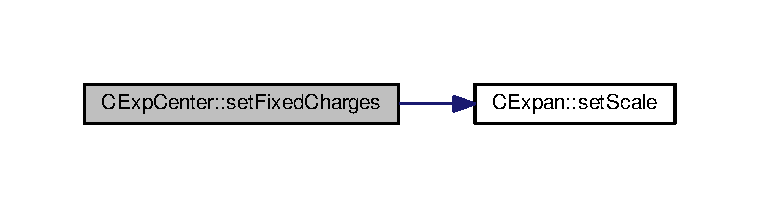
\includegraphics[width=350pt]{classCExpCenter_a44ea6f7aa0c0c37c721ed35e0b702703_cgraph}
\end{center}
\end{figure}


\hypertarget{classCExpCenter_a6d4be76f4a28b68eca9dcd4a778ca387}{\index{C\-Exp\-Center@{C\-Exp\-Center}!set\-Order@{set\-Order}}
\index{set\-Order@{set\-Order}!CExpCenter@{C\-Exp\-Center}}
\subsubsection[{set\-Order}]{\setlength{\rightskip}{0pt plus 5cm}void C\-Exp\-Center\-::set\-Order (
\begin{DoxyParamCaption}
\item[{const int}]{p, }
\item[{const {\bf C\-Rot\-Coeff} \&}]{rot}
\end{DoxyParamCaption}
)\hspace{0.3cm}{\ttfamily [inline]}}}\label{classCExpCenter_a6d4be76f4a28b68eca9dcd4a778ca387}
Exp\-Center function set\-Order a function that sets the order of the expansion and increases or decreases it accordingly 

Here is the call graph for this function\-:\nopagebreak
\begin{figure}[H]
\begin{center}
\leavevmode
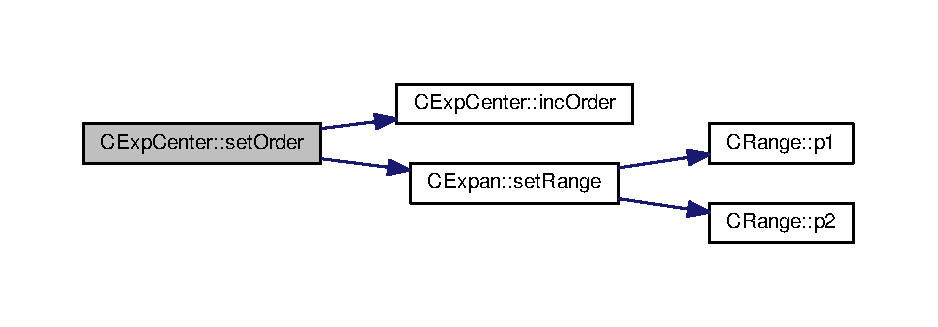
\includegraphics[width=350pt]{classCExpCenter_a6d4be76f4a28b68eca9dcd4a778ca387_cgraph}
\end{center}
\end{figure}




\subsection{Member Data Documentation}
\hypertarget{classCExpCenter_a9012e39bbe103cd93190156817b0efb4}{\index{C\-Exp\-Center@{C\-Exp\-Center}!m\-\_\-b\-Kappa@{m\-\_\-b\-Kappa}}
\index{m\-\_\-b\-Kappa@{m\-\_\-b\-Kappa}!CExpCenter@{C\-Exp\-Center}}
\subsubsection[{m\-\_\-b\-Kappa}]{\setlength{\rightskip}{0pt plus 5cm}bool C\-Exp\-Center\-::m\-\_\-b\-Kappa\hspace{0.3cm}{\ttfamily [protected]}}}\label{classCExpCenter_a9012e39bbe103cd93190156817b0efb4}
\hypertarget{classCExpCenter_a57a81c26f40939d189a88b82c77f16e8}{\index{C\-Exp\-Center@{C\-Exp\-Center}!m\-\_\-cen@{m\-\_\-cen}}
\index{m\-\_\-cen@{m\-\_\-cen}!CExpCenter@{C\-Exp\-Center}}
\subsubsection[{m\-\_\-cen}]{\setlength{\rightskip}{0pt plus 5cm}{\bf C\-Pnt} C\-Exp\-Center\-::m\-\_\-cen\hspace{0.3cm}{\ttfamily [protected]}}}\label{classCExpCenter_a57a81c26f40939d189a88b82c77f16e8}


An xyz of the center of the molecule in the standard frame. 

\hypertarget{classCExpCenter_a73b0d497d54258b3ab503167ae6f7e75}{\index{C\-Exp\-Center@{C\-Exp\-Center}!m\-\_\-cen\-Rot@{m\-\_\-cen\-Rot}}
\index{m\-\_\-cen\-Rot@{m\-\_\-cen\-Rot}!CExpCenter@{C\-Exp\-Center}}
\subsubsection[{m\-\_\-cen\-Rot}]{\setlength{\rightskip}{0pt plus 5cm}{\bf C\-Pnt} C\-Exp\-Center\-::m\-\_\-cen\-Rot\hspace{0.3cm}{\ttfamily [protected]}}}\label{classCExpCenter_a73b0d497d54258b3ab503167ae6f7e75}
\hypertarget{classCExpCenter_a834cd8238e3d5fd2b29a487d08f93978}{\index{C\-Exp\-Center@{C\-Exp\-Center}!m\-\_\-ch@{m\-\_\-ch}}
\index{m\-\_\-ch@{m\-\_\-ch}!CExpCenter@{C\-Exp\-Center}}
\subsubsection[{m\-\_\-ch}]{\setlength{\rightskip}{0pt plus 5cm}vector$<$double$>$ C\-Exp\-Center\-::m\-\_\-ch\hspace{0.3cm}{\ttfamily [protected]}}}\label{classCExpCenter_a834cd8238e3d5fd2b29a487d08f93978}
\hypertarget{classCExpCenter_a41728832a9a82eec510548f438e65734}{\index{C\-Exp\-Center@{C\-Exp\-Center}!m\-\_\-\-E@{m\-\_\-\-E}}
\index{m\-\_\-\-E@{m\-\_\-\-E}!CExpCenter@{C\-Exp\-Center}}
\subsubsection[{m\-\_\-\-E}]{\setlength{\rightskip}{0pt plus 5cm}{\bf C\-Mul\-Expan} C\-Exp\-Center\-::m\-\_\-\-E\hspace{0.3cm}{\ttfamily [protected]}}}\label{classCExpCenter_a41728832a9a82eec510548f438e65734}
\hypertarget{classCExpCenter_ae860d91bb83f5b31eff56694f6428e20}{\index{C\-Exp\-Center@{C\-Exp\-Center}!m\-\_\-g\-H@{m\-\_\-g\-H}}
\index{m\-\_\-g\-H@{m\-\_\-g\-H}!CExpCenter@{C\-Exp\-Center}}
\subsubsection[{m\-\_\-g\-H}]{\setlength{\rightskip}{0pt plus 5cm}{\bf C\-Grad\-Expan} C\-Exp\-Center\-::m\-\_\-g\-H\hspace{0.3cm}{\ttfamily [protected]}}}\label{classCExpCenter_ae860d91bb83f5b31eff56694f6428e20}
\hypertarget{classCExpCenter_a2ac196fbf3b2a5623553b4ecdc30cd7f}{\index{C\-Exp\-Center@{C\-Exp\-Center}!m\-\_\-g\-L\-H\-N@{m\-\_\-g\-L\-H\-N}}
\index{m\-\_\-g\-L\-H\-N@{m\-\_\-g\-L\-H\-N}!CExpCenter@{C\-Exp\-Center}}
\subsubsection[{m\-\_\-g\-L\-H\-N}]{\setlength{\rightskip}{0pt plus 5cm}{\bf C\-Grad\-Expan} C\-Exp\-Center\-::m\-\_\-g\-L\-H\-N\hspace{0.3cm}{\ttfamily [protected]}}}\label{classCExpCenter_a2ac196fbf3b2a5623553b4ecdc30cd7f}
\hypertarget{classCExpCenter_a6cf480aad64c9baf8a126d308ca63f85}{\index{C\-Exp\-Center@{C\-Exp\-Center}!m\-\_\-\-H@{m\-\_\-\-H}}
\index{m\-\_\-\-H@{m\-\_\-\-H}!CExpCenter@{C\-Exp\-Center}}
\subsubsection[{m\-\_\-\-H}]{\setlength{\rightskip}{0pt plus 5cm}{\bf C\-Mul\-Expan} C\-Exp\-Center\-::m\-\_\-\-H\hspace{0.3cm}{\ttfamily [protected]}}}\label{classCExpCenter_a6cf480aad64c9baf8a126d308ca63f85}


A multipole expansion of the effective polarization charges on sphere k of the exposed surf. 

\hypertarget{classCExpCenter_acfe6c4c74d9fd3069d00fef085eafbd8}{\index{C\-Exp\-Center@{C\-Exp\-Center}!m\-\_\-\-Hrot@{m\-\_\-\-Hrot}}
\index{m\-\_\-\-Hrot@{m\-\_\-\-Hrot}!CExpCenter@{C\-Exp\-Center}}
\subsubsection[{m\-\_\-\-Hrot}]{\setlength{\rightskip}{0pt plus 5cm}{\bf C\-Mul\-Expan} C\-Exp\-Center\-::m\-\_\-\-Hrot\hspace{0.3cm}{\ttfamily [protected]}}}\label{classCExpCenter_acfe6c4c74d9fd3069d00fef085eafbd8}


A rotated M\-P\-E of the effective polarization charges on sphere k of the exposed surf. 

\hypertarget{classCExpCenter_a7dcda3540f2ff0b3bfd668889ef1e95a}{\index{C\-Exp\-Center@{C\-Exp\-Center}!m\-\_\-id@{m\-\_\-id}}
\index{m\-\_\-id@{m\-\_\-id}!CExpCenter@{C\-Exp\-Center}}
\subsubsection[{m\-\_\-id}]{\setlength{\rightskip}{0pt plus 5cm}int C\-Exp\-Center\-::m\-\_\-id\hspace{0.3cm}{\ttfamily [protected]}}}\label{classCExpCenter_a7dcda3540f2ff0b3bfd668889ef1e95a}


An integer of the I\-D number of the C\-G sphere. 

\hypertarget{classCExpCenter_a2ebe2d840aaaa9329706514fa6957efa}{\index{C\-Exp\-Center@{C\-Exp\-Center}!m\-\_\-idiel@{m\-\_\-idiel}}
\index{m\-\_\-idiel@{m\-\_\-idiel}!CExpCenter@{C\-Exp\-Center}}
\subsubsection[{m\-\_\-idiel}]{\setlength{\rightskip}{0pt plus 5cm}double C\-Exp\-Center\-::m\-\_\-idiel\hspace{0.3cm}{\ttfamily [protected]}}}\label{classCExpCenter_a2ebe2d840aaaa9329706514fa6957efa}


A floating point of the molecule's interior dielectric constant. 

\hypertarget{classCExpCenter_aca58b7a93949d83d4b7883b54d0473e5}{\index{C\-Exp\-Center@{C\-Exp\-Center}!m\-\_\-kappa@{m\-\_\-kappa}}
\index{m\-\_\-kappa@{m\-\_\-kappa}!CExpCenter@{C\-Exp\-Center}}
\subsubsection[{m\-\_\-kappa}]{\setlength{\rightskip}{0pt plus 5cm}double C\-Exp\-Center\-::m\-\_\-kappa\hspace{0.3cm}{\ttfamily [static]}, {\ttfamily [protected]}}}\label{classCExpCenter_aca58b7a93949d83d4b7883b54d0473e5}


A floating point of the system's inverse debye length. 

\hypertarget{classCExpCenter_a89612776d4a057bdd4d36a7b4e10e647}{\index{C\-Exp\-Center@{C\-Exp\-Center}!m\-\_\-\-L\-S@{m\-\_\-\-L\-S}}
\index{m\-\_\-\-L\-S@{m\-\_\-\-L\-S}!CExpCenter@{C\-Exp\-Center}}
\subsubsection[{m\-\_\-\-L\-S}]{\setlength{\rightskip}{0pt plus 5cm}{\bf C\-Local\-Expan} C\-Exp\-Center\-::m\-\_\-\-L\-S\hspace{0.3cm}{\ttfamily [protected]}}}\label{classCExpCenter_a89612776d4a057bdd4d36a7b4e10e647}


only due to external source ( selected ) 

\hypertarget{classCExpCenter_aac9d9de905652a9d78115a1b53091bce}{\index{C\-Exp\-Center@{C\-Exp\-Center}!m\-\_\-lscale@{m\-\_\-lscale}}
\index{m\-\_\-lscale@{m\-\_\-lscale}!CExpCenter@{C\-Exp\-Center}}
\subsubsection[{m\-\_\-lscale}]{\setlength{\rightskip}{0pt plus 5cm}double C\-Exp\-Center\-::m\-\_\-lscale\hspace{0.3cm}{\ttfamily [protected]}}}\label{classCExpCenter_aac9d9de905652a9d78115a1b53091bce}


A floating point of the length scale of the current sphere, defaulted to m\-\_\-rad. 

\hypertarget{classCExpCenter_a7182695f02cc43411ebc67e64258a2ec}{\index{C\-Exp\-Center@{C\-Exp\-Center}!m\-\_\-mscale@{m\-\_\-mscale}}
\index{m\-\_\-mscale@{m\-\_\-mscale}!CExpCenter@{C\-Exp\-Center}}
\subsubsection[{m\-\_\-mscale}]{\setlength{\rightskip}{0pt plus 5cm}double C\-Exp\-Center\-::m\-\_\-mscale\hspace{0.3cm}{\ttfamily [protected]}}}\label{classCExpCenter_a7182695f02cc43411ebc67e64258a2ec}


A floating point of another length scale, defaulted to 1/m\-\_\-rad. 

\hypertarget{classCExpCenter_a49742562fd68129ab17aa716e6e661e8}{\index{C\-Exp\-Center@{C\-Exp\-Center}!m\-\_\-orient@{m\-\_\-orient}}
\index{m\-\_\-orient@{m\-\_\-orient}!CExpCenter@{C\-Exp\-Center}}
\subsubsection[{m\-\_\-orient}]{\setlength{\rightskip}{0pt plus 5cm}{\bf C\-Quat}$\ast$ C\-Exp\-Center\-::m\-\_\-orient\hspace{0.3cm}{\ttfamily [protected]}}}\label{classCExpCenter_a49742562fd68129ab17aa716e6e661e8}


A quaterion of the the current rotation of the molecule. 

\hypertarget{classCExpCenter_a2a3e3bc7c527c49e9ea4149dd33f4dba}{\index{C\-Exp\-Center@{C\-Exp\-Center}!m\-\_\-p@{m\-\_\-p}}
\index{m\-\_\-p@{m\-\_\-p}!CExpCenter@{C\-Exp\-Center}}
\subsubsection[{m\-\_\-p}]{\setlength{\rightskip}{0pt plus 5cm}int C\-Exp\-Center\-::m\-\_\-p\hspace{0.3cm}{\ttfamily [protected]}}}\label{classCExpCenter_a2a3e3bc7c527c49e9ea4149dd33f4dba}


An integer of the number of poles in the expansion. 

\hypertarget{classCExpCenter_a6d2bc11475081445ad8838d6deb889d3}{\index{C\-Exp\-Center@{C\-Exp\-Center}!m\-\_\-pos@{m\-\_\-pos}}
\index{m\-\_\-pos@{m\-\_\-pos}!CExpCenter@{C\-Exp\-Center}}
\subsubsection[{m\-\_\-pos}]{\setlength{\rightskip}{0pt plus 5cm}vector$<${\bf C\-Pnt}$>$ C\-Exp\-Center\-::m\-\_\-pos\hspace{0.3cm}{\ttfamily [protected]}}}\label{classCExpCenter_a6d2bc11475081445ad8838d6deb889d3}
\hypertarget{classCExpCenter_abc237f77679da4a21619a384e6ff4f6b}{\index{C\-Exp\-Center@{C\-Exp\-Center}!m\-\_\-rad@{m\-\_\-rad}}
\index{m\-\_\-rad@{m\-\_\-rad}!CExpCenter@{C\-Exp\-Center}}
\subsubsection[{m\-\_\-rad}]{\setlength{\rightskip}{0pt plus 5cm}double C\-Exp\-Center\-::m\-\_\-rad\hspace{0.3cm}{\ttfamily [protected]}}}\label{classCExpCenter_abc237f77679da4a21619a384e6ff4f6b}


A floating point of the current C\-G sphere's radius (a$^\wedge$(I,k)) 

\hypertarget{classCExpCenter_a4c494c322b3272097b3b6aadfc2959f6}{\index{C\-Exp\-Center@{C\-Exp\-Center}!m\-\_\-r\-E@{m\-\_\-r\-E}}
\index{m\-\_\-r\-E@{m\-\_\-r\-E}!CExpCenter@{C\-Exp\-Center}}
\subsubsection[{m\-\_\-r\-E}]{\setlength{\rightskip}{0pt plus 5cm}{\bf C\-Mul\-Expan} C\-Exp\-Center\-::m\-\_\-r\-E\hspace{0.3cm}{\ttfamily [protected]}}}\label{classCExpCenter_a4c494c322b3272097b3b6aadfc2959f6}
\hypertarget{classCExpCenter_a284a13e418738579f101ad9dc0af4dec}{\index{C\-Exp\-Center@{C\-Exp\-Center}!m\-\_\-rot@{m\-\_\-rot}}
\index{m\-\_\-rot@{m\-\_\-rot}!CExpCenter@{C\-Exp\-Center}}
\subsubsection[{m\-\_\-rot}]{\setlength{\rightskip}{0pt plus 5cm}{\bf C\-Rot\-Coeff}$\ast$ C\-Exp\-Center\-::m\-\_\-rot\hspace{0.3cm}{\ttfamily [protected]}}}\label{classCExpCenter_a284a13e418738579f101ad9dc0af4dec}
\hypertarget{classCExpCenter_a027b6ddd209098aa7f6c71f7b43367b3}{\index{C\-Exp\-Center@{C\-Exp\-Center}!m\-\_\-sdiel@{m\-\_\-sdiel}}
\index{m\-\_\-sdiel@{m\-\_\-sdiel}!CExpCenter@{C\-Exp\-Center}}
\subsubsection[{m\-\_\-sdiel}]{\setlength{\rightskip}{0pt plus 5cm}double C\-Exp\-Center\-::m\-\_\-sdiel\hspace{0.3cm}{\ttfamily [static]}, {\ttfamily [protected]}}}\label{classCExpCenter_a027b6ddd209098aa7f6c71f7b43367b3}


A floating point of the solvent dielectric constant. 



The documentation for this class was generated from the following files\-:\begin{DoxyCompactItemize}
\item 
\hyperlink{expcenter_8h}{expcenter.\-h}\item 
\hyperlink{expcenter_8cpp}{expcenter.\-cpp}\end{DoxyCompactItemize}

\hypertarget{classCFullSphereID}{\section{C\-Full\-Sphere\-I\-D Class Reference}
\label{classCFullSphereID}\index{C\-Full\-Sphere\-I\-D@{C\-Full\-Sphere\-I\-D}}
}


\hyperlink{classCFullSphereID}{C\-Full\-Sphere\-I\-D} class.  




{\ttfamily \#include $<$hash.\-h$>$}

\subsection*{Public Member Functions}
\begin{DoxyCompactItemize}
\item 
\hyperlink{classCFullSphereID_a19629df0afdd443b9caab10f89ea003e}{C\-Full\-Sphere\-I\-D} (int im\-\_\-, int is\-\_\-)
\item 
int \hyperlink{classCFullSphereID_a47e4f4ec9658b78cf19eb138b00387ae}{mid} () const 
\item 
int \hyperlink{classCFullSphereID_a92b739a3485beda70e2a20cca784fdef}{kid} () const 
\end{DoxyCompactItemize}
\subsection*{Public Attributes}
\begin{DoxyCompactItemize}
\item 
int \hyperlink{classCFullSphereID_a50ef0261eac4aa50470938544de904bf}{im}
\item 
int \hyperlink{classCFullSphereID_abfe8fd426e07fa9a9ebbeb3a9f21b498}{is}
\end{DoxyCompactItemize}


\subsection{Detailed Description}
\hyperlink{classCFullSphereID}{C\-Full\-Sphere\-I\-D} class. 

This class is a class containing all I\-D information about a sphere. 

\subsection{Constructor \& Destructor Documentation}
\hypertarget{classCFullSphereID_a19629df0afdd443b9caab10f89ea003e}{\index{C\-Full\-Sphere\-I\-D@{C\-Full\-Sphere\-I\-D}!C\-Full\-Sphere\-I\-D@{C\-Full\-Sphere\-I\-D}}
\index{C\-Full\-Sphere\-I\-D@{C\-Full\-Sphere\-I\-D}!CFullSphereID@{C\-Full\-Sphere\-I\-D}}
\subsubsection[{C\-Full\-Sphere\-I\-D}]{\setlength{\rightskip}{0pt plus 5cm}C\-Full\-Sphere\-I\-D\-::\-C\-Full\-Sphere\-I\-D (
\begin{DoxyParamCaption}
\item[{int}]{im\-\_\-, }
\item[{int}]{is\-\_\-}
\end{DoxyParamCaption}
)\hspace{0.3cm}{\ttfamily [inline]}}}\label{classCFullSphereID_a19629df0afdd443b9caab10f89ea003e}


\subsection{Member Function Documentation}
\hypertarget{classCFullSphereID_a92b739a3485beda70e2a20cca784fdef}{\index{C\-Full\-Sphere\-I\-D@{C\-Full\-Sphere\-I\-D}!kid@{kid}}
\index{kid@{kid}!CFullSphereID@{C\-Full\-Sphere\-I\-D}}
\subsubsection[{kid}]{\setlength{\rightskip}{0pt plus 5cm}int C\-Full\-Sphere\-I\-D\-::kid (
\begin{DoxyParamCaption}
{}
\end{DoxyParamCaption}
) const\hspace{0.3cm}{\ttfamily [inline]}}}\label{classCFullSphereID_a92b739a3485beda70e2a20cca784fdef}
\hypertarget{classCFullSphereID_a47e4f4ec9658b78cf19eb138b00387ae}{\index{C\-Full\-Sphere\-I\-D@{C\-Full\-Sphere\-I\-D}!mid@{mid}}
\index{mid@{mid}!CFullSphereID@{C\-Full\-Sphere\-I\-D}}
\subsubsection[{mid}]{\setlength{\rightskip}{0pt plus 5cm}int C\-Full\-Sphere\-I\-D\-::mid (
\begin{DoxyParamCaption}
{}
\end{DoxyParamCaption}
) const\hspace{0.3cm}{\ttfamily [inline]}}}\label{classCFullSphereID_a47e4f4ec9658b78cf19eb138b00387ae}


\subsection{Member Data Documentation}
\hypertarget{classCFullSphereID_a50ef0261eac4aa50470938544de904bf}{\index{C\-Full\-Sphere\-I\-D@{C\-Full\-Sphere\-I\-D}!im@{im}}
\index{im@{im}!CFullSphereID@{C\-Full\-Sphere\-I\-D}}
\subsubsection[{im}]{\setlength{\rightskip}{0pt plus 5cm}int C\-Full\-Sphere\-I\-D\-::im}}\label{classCFullSphereID_a50ef0261eac4aa50470938544de904bf}
\hypertarget{classCFullSphereID_abfe8fd426e07fa9a9ebbeb3a9f21b498}{\index{C\-Full\-Sphere\-I\-D@{C\-Full\-Sphere\-I\-D}!is@{is}}
\index{is@{is}!CFullSphereID@{C\-Full\-Sphere\-I\-D}}
\subsubsection[{is}]{\setlength{\rightskip}{0pt plus 5cm}int C\-Full\-Sphere\-I\-D\-::is}}\label{classCFullSphereID_abfe8fd426e07fa9a9ebbeb3a9f21b498}


The documentation for this class was generated from the following file\-:\begin{DoxyCompactItemize}
\item 
\hyperlink{hash_8h}{hash.\-h}\end{DoxyCompactItemize}

\hypertarget{classCFullSphereIDPair}{\section{C\-Full\-Sphere\-I\-D\-Pair Class Reference}
\label{classCFullSphereIDPair}\index{C\-Full\-Sphere\-I\-D\-Pair@{C\-Full\-Sphere\-I\-D\-Pair}}
}


\hyperlink{classCFullSphereIDPair}{C\-Full\-Sphere\-I\-D\-Pair} class.  




{\ttfamily \#include $<$hash.\-h$>$}

\subsection*{Public Member Functions}
\begin{DoxyCompactItemize}
\item 
\hyperlink{classCFullSphereIDPair_a9ce7c9ddb7371ee54413bf7a98288b80}{C\-Full\-Sphere\-I\-D\-Pair} (int im\-\_\-, int is\-\_\-, int jm\-\_\-, int js\-\_\-)
\end{DoxyCompactItemize}
\subsection*{Public Attributes}
\begin{DoxyCompactItemize}
\item 
int \hyperlink{classCFullSphereIDPair_a60629b97e6033458a0f053553e420a33}{im}
\item 
int \hyperlink{classCFullSphereIDPair_a8a6a419f8b195dad9eaf0efdef334160}{is}
\item 
int \hyperlink{classCFullSphereIDPair_a8d5d6e6632c185395142b1c0e9775f4b}{jm}
\item 
int \hyperlink{classCFullSphereIDPair_a5cf4df87753da2163a40a0bb08d50bd4}{js}
\end{DoxyCompactItemize}


\subsection{Detailed Description}
\hyperlink{classCFullSphereIDPair}{C\-Full\-Sphere\-I\-D\-Pair} class. 

This class is a class containing all I\-D information about a pair of spheres. 

\subsection{Constructor \& Destructor Documentation}
\hypertarget{classCFullSphereIDPair_a9ce7c9ddb7371ee54413bf7a98288b80}{\index{C\-Full\-Sphere\-I\-D\-Pair@{C\-Full\-Sphere\-I\-D\-Pair}!C\-Full\-Sphere\-I\-D\-Pair@{C\-Full\-Sphere\-I\-D\-Pair}}
\index{C\-Full\-Sphere\-I\-D\-Pair@{C\-Full\-Sphere\-I\-D\-Pair}!CFullSphereIDPair@{C\-Full\-Sphere\-I\-D\-Pair}}
\subsubsection[{C\-Full\-Sphere\-I\-D\-Pair}]{\setlength{\rightskip}{0pt plus 5cm}C\-Full\-Sphere\-I\-D\-Pair\-::\-C\-Full\-Sphere\-I\-D\-Pair (
\begin{DoxyParamCaption}
\item[{int}]{im\-\_\-, }
\item[{int}]{is\-\_\-, }
\item[{int}]{jm\-\_\-, }
\item[{int}]{js\-\_\-}
\end{DoxyParamCaption}
)\hspace{0.3cm}{\ttfamily [inline]}}}\label{classCFullSphereIDPair_a9ce7c9ddb7371ee54413bf7a98288b80}


\subsection{Member Data Documentation}
\hypertarget{classCFullSphereIDPair_a60629b97e6033458a0f053553e420a33}{\index{C\-Full\-Sphere\-I\-D\-Pair@{C\-Full\-Sphere\-I\-D\-Pair}!im@{im}}
\index{im@{im}!CFullSphereIDPair@{C\-Full\-Sphere\-I\-D\-Pair}}
\subsubsection[{im}]{\setlength{\rightskip}{0pt plus 5cm}int C\-Full\-Sphere\-I\-D\-Pair\-::im}}\label{classCFullSphereIDPair_a60629b97e6033458a0f053553e420a33}
\hypertarget{classCFullSphereIDPair_a8a6a419f8b195dad9eaf0efdef334160}{\index{C\-Full\-Sphere\-I\-D\-Pair@{C\-Full\-Sphere\-I\-D\-Pair}!is@{is}}
\index{is@{is}!CFullSphereIDPair@{C\-Full\-Sphere\-I\-D\-Pair}}
\subsubsection[{is}]{\setlength{\rightskip}{0pt plus 5cm}int C\-Full\-Sphere\-I\-D\-Pair\-::is}}\label{classCFullSphereIDPair_a8a6a419f8b195dad9eaf0efdef334160}
\hypertarget{classCFullSphereIDPair_a8d5d6e6632c185395142b1c0e9775f4b}{\index{C\-Full\-Sphere\-I\-D\-Pair@{C\-Full\-Sphere\-I\-D\-Pair}!jm@{jm}}
\index{jm@{jm}!CFullSphereIDPair@{C\-Full\-Sphere\-I\-D\-Pair}}
\subsubsection[{jm}]{\setlength{\rightskip}{0pt plus 5cm}int C\-Full\-Sphere\-I\-D\-Pair\-::jm}}\label{classCFullSphereIDPair_a8d5d6e6632c185395142b1c0e9775f4b}
\hypertarget{classCFullSphereIDPair_a5cf4df87753da2163a40a0bb08d50bd4}{\index{C\-Full\-Sphere\-I\-D\-Pair@{C\-Full\-Sphere\-I\-D\-Pair}!js@{js}}
\index{js@{js}!CFullSphereIDPair@{C\-Full\-Sphere\-I\-D\-Pair}}
\subsubsection[{js}]{\setlength{\rightskip}{0pt plus 5cm}int C\-Full\-Sphere\-I\-D\-Pair\-::js}}\label{classCFullSphereIDPair_a5cf4df87753da2163a40a0bb08d50bd4}


The documentation for this class was generated from the following file\-:\begin{DoxyCompactItemize}
\item 
\hyperlink{hash_8h}{hash.\-h}\end{DoxyCompactItemize}

\hypertarget{classCGradExpan}{\section{C\-Grad\-Expan Class Reference}
\label{classCGradExpan}\index{C\-Grad\-Expan@{C\-Grad\-Expan}}
}


{\ttfamily \#include $<$triexpan.\-h$>$}



Inheritance diagram for C\-Grad\-Expan\-:\nopagebreak
\begin{figure}[H]
\begin{center}
\leavevmode
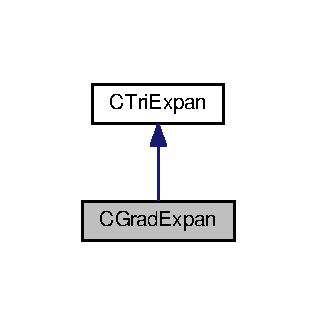
\includegraphics[width=152pt]{classCGradExpan__inherit__graph}
\end{center}
\end{figure}


Collaboration diagram for C\-Grad\-Expan\-:\nopagebreak
\begin{figure}[H]
\begin{center}
\leavevmode
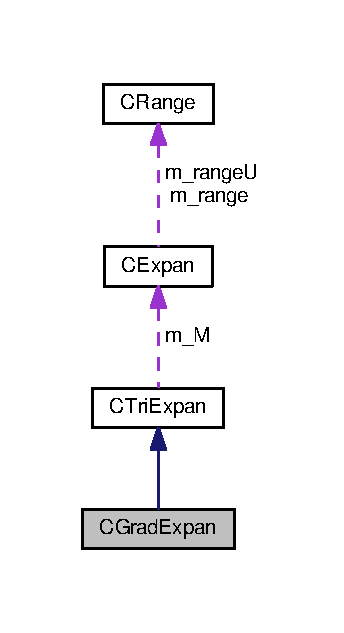
\includegraphics[width=165pt]{classCGradExpan__coll__graph}
\end{center}
\end{figure}
\subsection*{Public Member Functions}
\begin{DoxyCompactItemize}
\item 
\hyperlink{classCGradExpan_a4ddece353cfe42d5e43da09f8897d74a}{C\-Grad\-Expan} (int p=0, int res=\hyperlink{expansion_8h_ac23f9c13c5d07d9ce386f7a830c35e5a}{N\-\_\-\-P\-O\-L\-E\-S})
\item 
\hyperlink{classCGradExpan_a3c7cd4c78753f7809c5adb15cccf8ddb}{C\-Grad\-Expan} (const \hyperlink{classCPnt}{C\-Pnt} $\ast$g, const vector$<$ \hyperlink{classCPnt}{C\-Pnt} $>$ \&pos, int p, bool b\-Kappa, \hyperlink{util_8h_a5821460e95a0800cf9f24c38915cbbde}{R\-E\-A\-L} scale, bool b\-Multipole)
\item 
\hyperlink{classCGradExpan_a48acf31a1b0f93096b36979b0a183c6e}{C\-Grad\-Expan} (const \hyperlink{classCTriExpan}{C\-Tri\-Expan} \&G)
\item 
\hyperlink{classCGradExpan}{C\-Grad\-Expan} \hyperlink{classCGradExpan_a3cde1e2392ceb3319d808717da1cf990}{sph\-To\-Cart} (const \hyperlink{classCPnt}{C\-Pnt} $\ast$R)
\end{DoxyCompactItemize}
\subsection*{Additional Inherited Members}


\subsection{Detailed Description}

\begin{DoxyItemize}
\item \hyperlink{classCGradExpan}{C\-Grad\-Expan}\-: Not sure whether necessary but define anyway 
\end{DoxyItemize}

\subsection{Constructor \& Destructor Documentation}
\hypertarget{classCGradExpan_a4ddece353cfe42d5e43da09f8897d74a}{\index{C\-Grad\-Expan@{C\-Grad\-Expan}!C\-Grad\-Expan@{C\-Grad\-Expan}}
\index{C\-Grad\-Expan@{C\-Grad\-Expan}!CGradExpan@{C\-Grad\-Expan}}
\subsubsection[{C\-Grad\-Expan}]{\setlength{\rightskip}{0pt plus 5cm}C\-Grad\-Expan\-::\-C\-Grad\-Expan (
\begin{DoxyParamCaption}
\item[{int}]{p = {\ttfamily 0}, }
\item[{int}]{res = {\ttfamily {\bf N\-\_\-\-P\-O\-L\-E\-S}}}
\end{DoxyParamCaption}
)\hspace{0.3cm}{\ttfamily [inline]}}}\label{classCGradExpan_a4ddece353cfe42d5e43da09f8897d74a}
\hypertarget{classCGradExpan_a3c7cd4c78753f7809c5adb15cccf8ddb}{\index{C\-Grad\-Expan@{C\-Grad\-Expan}!C\-Grad\-Expan@{C\-Grad\-Expan}}
\index{C\-Grad\-Expan@{C\-Grad\-Expan}!CGradExpan@{C\-Grad\-Expan}}
\subsubsection[{C\-Grad\-Expan}]{\setlength{\rightskip}{0pt plus 5cm}C\-Grad\-Expan\-::\-C\-Grad\-Expan (
\begin{DoxyParamCaption}
\item[{const {\bf C\-Pnt} $\ast$}]{g, }
\item[{const vector$<$ {\bf C\-Pnt} $>$ \&}]{pos, }
\item[{int}]{p, }
\item[{bool}]{b\-Kappa, }
\item[{{\bf R\-E\-A\-L}}]{scale, }
\item[{bool}]{b\-Multipole}
\end{DoxyParamCaption}
)}}\label{classCGradExpan_a3c7cd4c78753f7809c5adb15cccf8ddb}
\hyperlink{classCGradExpan}{C\-Grad\-Expan} class constructor. Makes a gradient expansion class 

Here is the call graph for this function\-:\nopagebreak
\begin{figure}[H]
\begin{center}
\leavevmode
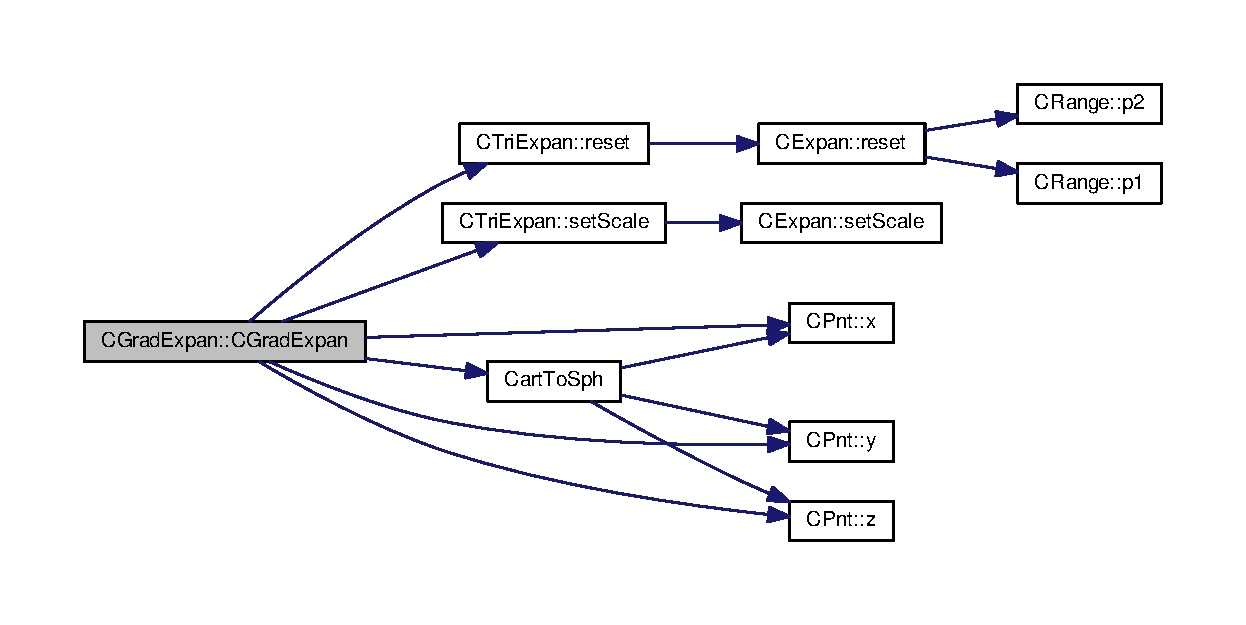
\includegraphics[width=350pt]{classCGradExpan_a3c7cd4c78753f7809c5adb15cccf8ddb_cgraph}
\end{center}
\end{figure}


\hypertarget{classCGradExpan_a48acf31a1b0f93096b36979b0a183c6e}{\index{C\-Grad\-Expan@{C\-Grad\-Expan}!C\-Grad\-Expan@{C\-Grad\-Expan}}
\index{C\-Grad\-Expan@{C\-Grad\-Expan}!CGradExpan@{C\-Grad\-Expan}}
\subsubsection[{C\-Grad\-Expan}]{\setlength{\rightskip}{0pt plus 5cm}C\-Grad\-Expan\-::\-C\-Grad\-Expan (
\begin{DoxyParamCaption}
\item[{const {\bf C\-Tri\-Expan} \&}]{G}
\end{DoxyParamCaption}
)\hspace{0.3cm}{\ttfamily [inline]}}}\label{classCGradExpan_a48acf31a1b0f93096b36979b0a183c6e}


\subsection{Member Function Documentation}
\hypertarget{classCGradExpan_a3cde1e2392ceb3319d808717da1cf990}{\index{C\-Grad\-Expan@{C\-Grad\-Expan}!sph\-To\-Cart@{sph\-To\-Cart}}
\index{sph\-To\-Cart@{sph\-To\-Cart}!CGradExpan@{C\-Grad\-Expan}}
\subsubsection[{sph\-To\-Cart}]{\setlength{\rightskip}{0pt plus 5cm}{\bf C\-Grad\-Expan} C\-Grad\-Expan\-::sph\-To\-Cart (
\begin{DoxyParamCaption}
\item[{const {\bf C\-Pnt} $\ast$}]{R}
\end{DoxyParamCaption}
)\hspace{0.3cm}{\ttfamily [inline]}}}\label{classCGradExpan_a3cde1e2392ceb3319d808717da1cf990}

\begin{DoxyItemize}
\item Convert spherical derivatives to cartesian coords 
\end{DoxyItemize}

Here is the call graph for this function\-:\nopagebreak
\begin{figure}[H]
\begin{center}
\leavevmode
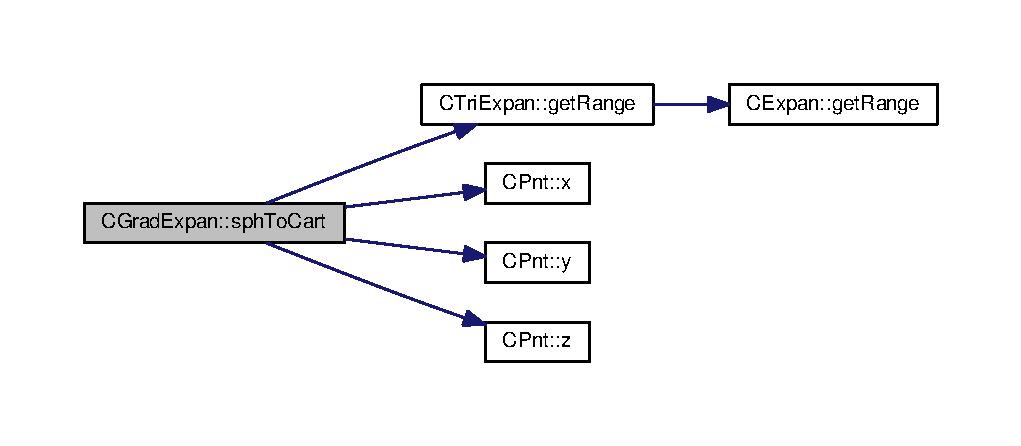
\includegraphics[width=350pt]{classCGradExpan_a3cde1e2392ceb3319d808717da1cf990_cgraph}
\end{center}
\end{figure}




The documentation for this class was generated from the following files\-:\begin{DoxyCompactItemize}
\item 
\hyperlink{triexpan_8h}{triexpan.\-h}\item 
\hyperlink{triexpan_8cpp}{triexpan.\-cpp}\end{DoxyCompactItemize}

\hypertarget{structclassCompareCFullSphereID}{\section{class\-Compare\-C\-Full\-Sphere\-I\-D Struct Reference}
\label{structclassCompareCFullSphereID}\index{class\-Compare\-C\-Full\-Sphere\-I\-D@{class\-Compare\-C\-Full\-Sphere\-I\-D}}
}


\hyperlink{structclassCompareCFullSphereID}{class\-Compare\-C\-Full\-Sphere\-I\-D} class  




{\ttfamily \#include $<$hash.\-h$>$}

\subsection*{Public Member Functions}
\begin{DoxyCompactItemize}
\item 
bool \hyperlink{structclassCompareCFullSphereID_a4c269ff95e0dda8eddfc1ebf4ede4db4}{operator()} (const \hyperlink{classCFullSphereID}{C\-Full\-Sphere\-I\-D} \&lhs, const \hyperlink{classCFullSphereID}{C\-Full\-Sphere\-I\-D} \&rhs)
\end{DoxyCompactItemize}


\subsection{Detailed Description}
\hyperlink{structclassCompareCFullSphereID}{class\-Compare\-C\-Full\-Sphere\-I\-D} class 

This class is a class containing information about the relationship between two sphere's I\-D objects. Returns true if the first one is smaller. False if the second one is smaller. And otherwise compares the objects first spheres. 

\subsection{Member Function Documentation}
\hypertarget{structclassCompareCFullSphereID_a4c269ff95e0dda8eddfc1ebf4ede4db4}{\index{class\-Compare\-C\-Full\-Sphere\-I\-D@{class\-Compare\-C\-Full\-Sphere\-I\-D}!operator()@{operator()}}
\index{operator()@{operator()}!classCompareCFullSphereID@{class\-Compare\-C\-Full\-Sphere\-I\-D}}
\subsubsection[{operator()}]{\setlength{\rightskip}{0pt plus 5cm}bool class\-Compare\-C\-Full\-Sphere\-I\-D\-::operator() (
\begin{DoxyParamCaption}
\item[{const {\bf C\-Full\-Sphere\-I\-D} \&}]{lhs, }
\item[{const {\bf C\-Full\-Sphere\-I\-D} \&}]{rhs}
\end{DoxyParamCaption}
)\hspace{0.3cm}{\ttfamily [inline]}}}\label{structclassCompareCFullSphereID_a4c269ff95e0dda8eddfc1ebf4ede4db4}


The documentation for this struct was generated from the following file\-:\begin{DoxyCompactItemize}
\item 
\hyperlink{hash_8h}{hash.\-h}\end{DoxyCompactItemize}

\hypertarget{structclassCompareCFullSphereIDPair}{\section{class\-Compare\-C\-Full\-Sphere\-I\-D\-Pair Struct Reference}
\label{structclassCompareCFullSphereIDPair}\index{class\-Compare\-C\-Full\-Sphere\-I\-D\-Pair@{class\-Compare\-C\-Full\-Sphere\-I\-D\-Pair}}
}


\hyperlink{structclassCompareCFullSphereIDPair}{class\-Compare\-C\-Full\-Sphere\-I\-D\-Pair} class  




{\ttfamily \#include $<$hash.\-h$>$}

\subsection*{Public Member Functions}
\begin{DoxyCompactItemize}
\item 
bool \hyperlink{structclassCompareCFullSphereIDPair_a407ccf0e6ce1692d0ab9b24fdbe526ba}{operator()} (const \hyperlink{classCFullSphereIDPair}{C\-Full\-Sphere\-I\-D\-Pair} \&lhs, const \hyperlink{classCFullSphereIDPair}{C\-Full\-Sphere\-I\-D\-Pair} \&rhs)
\end{DoxyCompactItemize}


\subsection{Detailed Description}
\hyperlink{structclassCompareCFullSphereIDPair}{class\-Compare\-C\-Full\-Sphere\-I\-D\-Pair} class 

This class is a class containing information about the relationship between two sphere's I\-D objects. Returns true if the first one is smaller. False if the second one is smaller. And otherwise compares the objects first spheres. 

\subsection{Member Function Documentation}
\hypertarget{structclassCompareCFullSphereIDPair_a407ccf0e6ce1692d0ab9b24fdbe526ba}{\index{class\-Compare\-C\-Full\-Sphere\-I\-D\-Pair@{class\-Compare\-C\-Full\-Sphere\-I\-D\-Pair}!operator()@{operator()}}
\index{operator()@{operator()}!classCompareCFullSphereIDPair@{class\-Compare\-C\-Full\-Sphere\-I\-D\-Pair}}
\subsubsection[{operator()}]{\setlength{\rightskip}{0pt plus 5cm}bool class\-Compare\-C\-Full\-Sphere\-I\-D\-Pair\-::operator() (
\begin{DoxyParamCaption}
\item[{const {\bf C\-Full\-Sphere\-I\-D\-Pair} \&}]{lhs, }
\item[{const {\bf C\-Full\-Sphere\-I\-D\-Pair} \&}]{rhs}
\end{DoxyParamCaption}
)\hspace{0.3cm}{\ttfamily [inline]}}}\label{structclassCompareCFullSphereIDPair_a407ccf0e6ce1692d0ab9b24fdbe526ba}


The documentation for this struct was generated from the following file\-:\begin{DoxyCompactItemize}
\item 
\hyperlink{hash_8h}{hash.\-h}\end{DoxyCompactItemize}

\hypertarget{structclassCompareCSphereIDPair}{\section{class\-Compare\-C\-Sphere\-I\-D\-Pair Struct Reference}
\label{structclassCompareCSphereIDPair}\index{class\-Compare\-C\-Sphere\-I\-D\-Pair@{class\-Compare\-C\-Sphere\-I\-D\-Pair}}
}


\hyperlink{structclassCompareCSphereIDPair}{class\-Compare\-C\-Sphere\-I\-D\-Pair} class  




{\ttfamily \#include $<$hash.\-h$>$}

\subsection*{Public Member Functions}
\begin{DoxyCompactItemize}
\item 
bool \hyperlink{structclassCompareCSphereIDPair_aee7fd4dab46a0c6e7ed1f1ccd3d5eea2}{operator()} (const \hyperlink{classCSphereIDPair}{C\-Sphere\-I\-D\-Pair} \&lhs, const \hyperlink{classCSphereIDPair}{C\-Sphere\-I\-D\-Pair} \&rhs)
\end{DoxyCompactItemize}


\subsection{Detailed Description}
\hyperlink{structclassCompareCSphereIDPair}{class\-Compare\-C\-Sphere\-I\-D\-Pair} class 

This class is a class containing information about the relationship between two sphere's I\-D objects. Returns true if the first one is smaller. False if the second one is smaller. And otherwise compares the objects first spheres. 

\subsection{Member Function Documentation}
\hypertarget{structclassCompareCSphereIDPair_aee7fd4dab46a0c6e7ed1f1ccd3d5eea2}{\index{class\-Compare\-C\-Sphere\-I\-D\-Pair@{class\-Compare\-C\-Sphere\-I\-D\-Pair}!operator()@{operator()}}
\index{operator()@{operator()}!classCompareCSphereIDPair@{class\-Compare\-C\-Sphere\-I\-D\-Pair}}
\subsubsection[{operator()}]{\setlength{\rightskip}{0pt plus 5cm}bool class\-Compare\-C\-Sphere\-I\-D\-Pair\-::operator() (
\begin{DoxyParamCaption}
\item[{const {\bf C\-Sphere\-I\-D\-Pair} \&}]{lhs, }
\item[{const {\bf C\-Sphere\-I\-D\-Pair} \&}]{rhs}
\end{DoxyParamCaption}
)\hspace{0.3cm}{\ttfamily [inline]}}}\label{structclassCompareCSphereIDPair_aee7fd4dab46a0c6e7ed1f1ccd3d5eea2}


The documentation for this struct was generated from the following file\-:\begin{DoxyCompactItemize}
\item 
\hyperlink{hash_8h}{hash.\-h}\end{DoxyCompactItemize}

\hypertarget{classCLExpan}{\section{C\-L\-Expan Class Reference}
\label{classCLExpan}\index{C\-L\-Expan@{C\-L\-Expan}}
}


{\ttfamily \#include $<$expansion.\-h$>$}



Inheritance diagram for C\-L\-Expan\-:\nopagebreak
\begin{figure}[H]
\begin{center}
\leavevmode
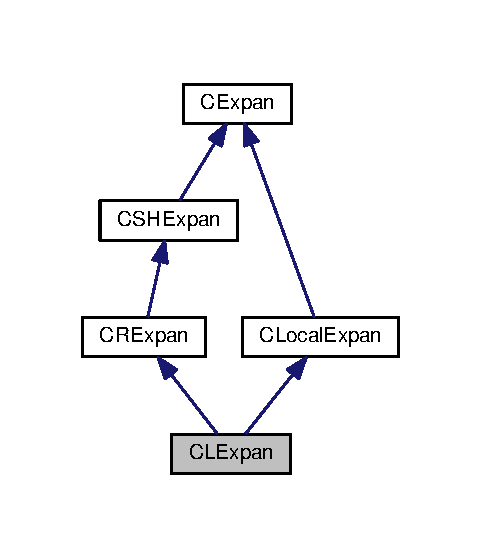
\includegraphics[width=231pt]{classCLExpan__inherit__graph}
\end{center}
\end{figure}


Collaboration diagram for C\-L\-Expan\-:\nopagebreak
\begin{figure}[H]
\begin{center}
\leavevmode
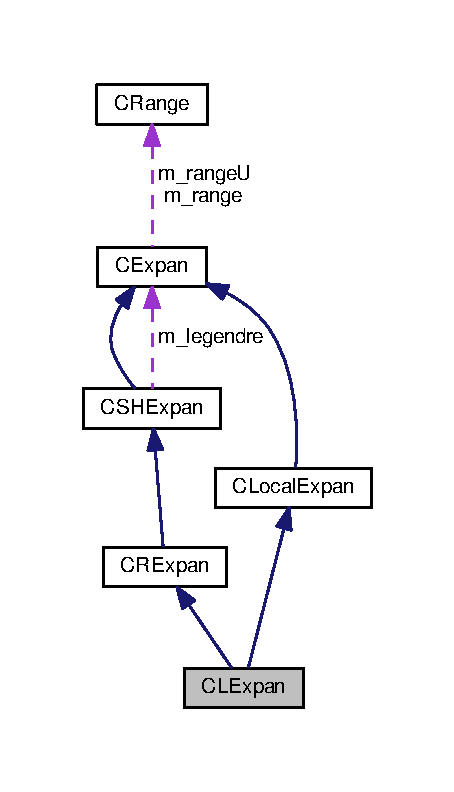
\includegraphics[width=218pt]{classCLExpan__coll__graph}
\end{center}
\end{figure}
\subsection*{Public Member Functions}
\begin{DoxyCompactItemize}
\item 
\hyperlink{classCLExpan_a70aa27dc869e15334f170a5ce6de0060}{C\-L\-Expan} (\hyperlink{util_8h_a5821460e95a0800cf9f24c38915cbbde}{R\-E\-A\-L} ch, const \hyperlink{classCSpPnt}{C\-Sp\-Pnt} \&spos, bool b\-Kappa, int p, double scale=1.\-0)
\item 
\hyperlink{classCLExpan_abdad541bae891eaf8c8c6c5e1910c339}{C\-L\-Expan} (const \hyperlink{classCLExpan}{C\-L\-Expan} \&L)
\item 
virtual void \hyperlink{classCLExpan_a965e320a6287db9e6f2b79ad0e0c7861}{init} ()
\item 
const \hyperlink{classCLExpan}{C\-L\-Expan} \& \hyperlink{classCLExpan_af787b152eb9c35ed7e554d9d68519c4a}{operator=} (const \hyperlink{classCLExpan}{C\-L\-Expan} \&M)
\item 
virtual \hyperlink{classCExpan}{C\-Expan} \hyperlink{classCLExpan_acdececf909b426f67e079418ff01bc45}{d\-Mdr} () const 
\end{DoxyCompactItemize}


Collaboration diagram for C\-Local\-Expan\-:\nopagebreak
\begin{figure}[H]
\begin{center}
\leavevmode
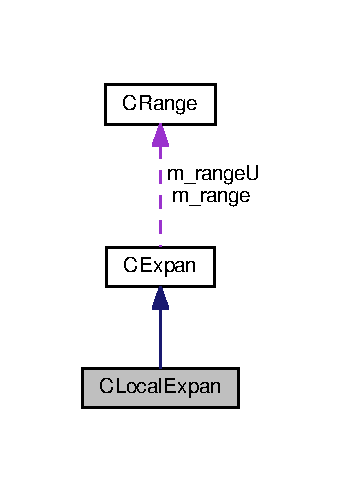
\includegraphics[width=166pt]{classCLocalExpan__coll__graph}
\end{center}
\end{figure}
\subsection*{Public Member Functions}
\begin{DoxyCompactItemize}
\item 
\hyperlink{classCLocalExpan_a16c516c3997efee3e4db44e826af7a74}{C\-Local\-Expan} (const double $\ast$v, const \hyperlink{classCRange}{C\-Range} \&range, double scale=1.\-0)
\item 
\hyperlink{classCLocalExpan_a1d8189f26cb590dbf2ed84724784277a}{C\-Local\-Expan} (const vector$<$ \hyperlink{util_8h_a5821460e95a0800cf9f24c38915cbbde}{R\-E\-A\-L} $>$ M, const \hyperlink{classCRange}{C\-Range} \&range, double scale=1.\-0)
\item 
\hyperlink{classCLocalExpan_aecedf22ca8c5169f0c064b0b5a7e772d}{C\-Local\-Expan} (const vector$<$ \hyperlink{util_8h_a5821460e95a0800cf9f24c38915cbbde}{R\-E\-A\-L} $>$ \&ch, const vector$<$ \hyperlink{classCPnt}{C\-Pnt} $>$ \&pos, int p, bool b\-Kappa, \hyperlink{util_8h_a5821460e95a0800cf9f24c38915cbbde}{R\-E\-A\-L} scale)
\item 
\hyperlink{classCLocalExpan_aefec98860c64c14640ff7c1099687ced}{C\-Local\-Expan} (const \hyperlink{util_8h_a5821460e95a0800cf9f24c38915cbbde}{R\-E\-A\-L} $\ast$ch, const vector$<$ \hyperlink{classCPnt}{C\-Pnt} $>$ \&pos, int p, bool b\-Kappa, \hyperlink{util_8h_a5821460e95a0800cf9f24c38915cbbde}{R\-E\-A\-L} scale)
\item 
\hyperlink{classCLocalExpan_a70a4260de05dfbc5a98e0660e10269ce}{C\-Local\-Expan} (int p=0)
\item 
\hyperlink{classCLocalExpan_a09cdbca66aa809acd1a4dc15387982f1}{C\-Local\-Expan} (const \hyperlink{classCRange}{C\-Range} \&range, \hyperlink{util_8h_a5821460e95a0800cf9f24c38915cbbde}{R\-E\-A\-L} scale=1.\-0)
\end{DoxyCompactItemize}
\subsection*{Friends}
\begin{DoxyCompactItemize}
\item 
\hyperlink{util_8h_a5821460e95a0800cf9f24c38915cbbde}{R\-E\-A\-L} \hyperlink{classCLocalExpan_a020c55be9514911fc8ecde0a8d81a919}{inprod} (const \hyperlink{classCMulExpan}{C\-Mul\-Expan} \&M, const \hyperlink{classCLocalExpan}{C\-Local\-Expan} \&L)
\end{DoxyCompactItemize}
\subsection*{Additional Inherited Members}


\subsection{Detailed Description}
The \hyperlink{classCLocalExpan}{C\-Local\-Expan} class

The \hyperlink{classCLocalExpan}{C\-Local\-Expan} class contains information about general local expansion class. 

\subsection{Constructor \& Destructor Documentation}
\hypertarget{classCLocalExpan_a16c516c3997efee3e4db44e826af7a74}{\index{C\-Local\-Expan@{C\-Local\-Expan}!C\-Local\-Expan@{C\-Local\-Expan}}
\index{C\-Local\-Expan@{C\-Local\-Expan}!CLocalExpan@{C\-Local\-Expan}}
\subsubsection[{C\-Local\-Expan}]{\setlength{\rightskip}{0pt plus 5cm}C\-Local\-Expan\-::\-C\-Local\-Expan (
\begin{DoxyParamCaption}
\item[{const double $\ast$}]{v, }
\item[{const {\bf C\-Range} \&}]{range, }
\item[{double}]{scale = {\ttfamily 1.0}}
\end{DoxyParamCaption}
)\hspace{0.3cm}{\ttfamily [inline]}}}\label{classCLocalExpan_a16c516c3997efee3e4db44e826af7a74}
\hypertarget{classCLocalExpan_a1d8189f26cb590dbf2ed84724784277a}{\index{C\-Local\-Expan@{C\-Local\-Expan}!C\-Local\-Expan@{C\-Local\-Expan}}
\index{C\-Local\-Expan@{C\-Local\-Expan}!CLocalExpan@{C\-Local\-Expan}}
\subsubsection[{C\-Local\-Expan}]{\setlength{\rightskip}{0pt plus 5cm}C\-Local\-Expan\-::\-C\-Local\-Expan (
\begin{DoxyParamCaption}
\item[{const vector$<$ {\bf R\-E\-A\-L} $>$}]{M, }
\item[{const {\bf C\-Range} \&}]{range, }
\item[{double}]{scale = {\ttfamily 1.0}}
\end{DoxyParamCaption}
)\hspace{0.3cm}{\ttfamily [inline]}}}\label{classCLocalExpan_a1d8189f26cb590dbf2ed84724784277a}
\hypertarget{classCLocalExpan_aecedf22ca8c5169f0c064b0b5a7e772d}{\index{C\-Local\-Expan@{C\-Local\-Expan}!C\-Local\-Expan@{C\-Local\-Expan}}
\index{C\-Local\-Expan@{C\-Local\-Expan}!CLocalExpan@{C\-Local\-Expan}}
\subsubsection[{C\-Local\-Expan}]{\setlength{\rightskip}{0pt plus 5cm}C\-Local\-Expan\-::\-C\-Local\-Expan (
\begin{DoxyParamCaption}
\item[{const vector$<$ {\bf R\-E\-A\-L} $>$ \&}]{ch, }
\item[{const vector$<$ {\bf C\-Pnt} $>$ \&}]{pos, }
\item[{int}]{p, }
\item[{bool}]{b\-Kappa, }
\item[{{\bf R\-E\-A\-L}}]{scale}
\end{DoxyParamCaption}
)}}\label{classCLocalExpan_aecedf22ca8c5169f0c064b0b5a7e772d}
Initialize a local expansion object 

Here is the call graph for this function\-:\nopagebreak
\begin{figure}[H]
\begin{center}
\leavevmode
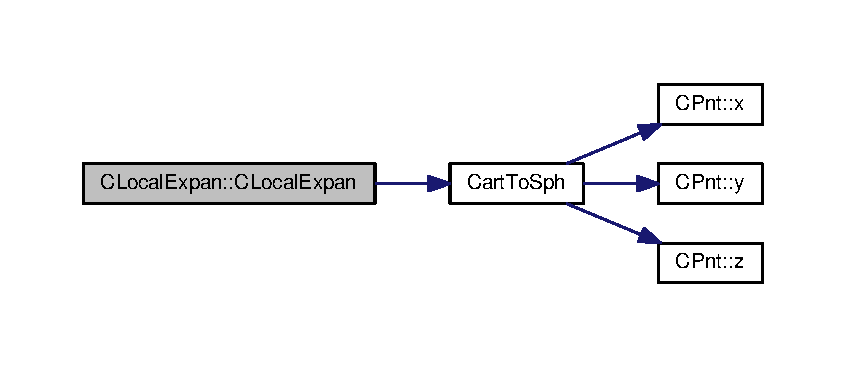
\includegraphics[width=350pt]{classCLocalExpan_aecedf22ca8c5169f0c064b0b5a7e772d_cgraph}
\end{center}
\end{figure}


\hypertarget{classCLocalExpan_aefec98860c64c14640ff7c1099687ced}{\index{C\-Local\-Expan@{C\-Local\-Expan}!C\-Local\-Expan@{C\-Local\-Expan}}
\index{C\-Local\-Expan@{C\-Local\-Expan}!CLocalExpan@{C\-Local\-Expan}}
\subsubsection[{C\-Local\-Expan}]{\setlength{\rightskip}{0pt plus 5cm}C\-Local\-Expan\-::\-C\-Local\-Expan (
\begin{DoxyParamCaption}
\item[{const {\bf R\-E\-A\-L} $\ast$}]{ch, }
\item[{const vector$<$ {\bf C\-Pnt} $>$ \&}]{pos, }
\item[{int}]{p, }
\item[{bool}]{b\-Kappa, }
\item[{{\bf R\-E\-A\-L}}]{scale}
\end{DoxyParamCaption}
)}}\label{classCLocalExpan_aefec98860c64c14640ff7c1099687ced}
Construct a local expansion for a set of charges 

Here is the call graph for this function\-:\nopagebreak
\begin{figure}[H]
\begin{center}
\leavevmode
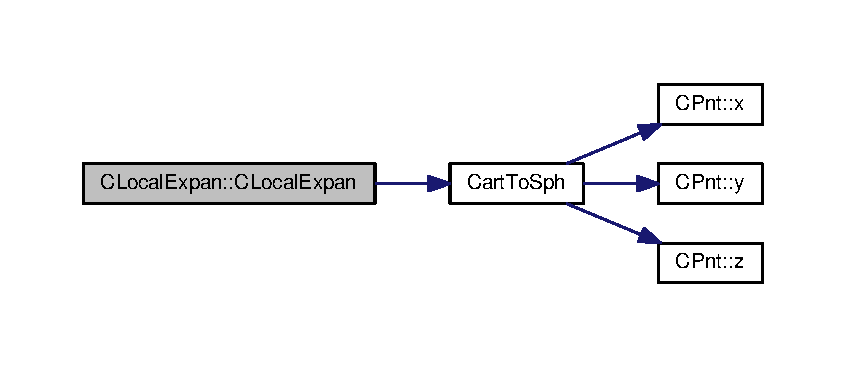
\includegraphics[width=350pt]{classCLocalExpan_aefec98860c64c14640ff7c1099687ced_cgraph}
\end{center}
\end{figure}


\hypertarget{classCLocalExpan_a70a4260de05dfbc5a98e0660e10269ce}{\index{C\-Local\-Expan@{C\-Local\-Expan}!C\-Local\-Expan@{C\-Local\-Expan}}
\index{C\-Local\-Expan@{C\-Local\-Expan}!CLocalExpan@{C\-Local\-Expan}}
\subsubsection[{C\-Local\-Expan}]{\setlength{\rightskip}{0pt plus 5cm}C\-Local\-Expan\-::\-C\-Local\-Expan (
\begin{DoxyParamCaption}
\item[{int}]{p = {\ttfamily 0}}
\end{DoxyParamCaption}
)\hspace{0.3cm}{\ttfamily [inline]}}}\label{classCLocalExpan_a70a4260de05dfbc5a98e0660e10269ce}
\hypertarget{classCLocalExpan_a09cdbca66aa809acd1a4dc15387982f1}{\index{C\-Local\-Expan@{C\-Local\-Expan}!C\-Local\-Expan@{C\-Local\-Expan}}
\index{C\-Local\-Expan@{C\-Local\-Expan}!CLocalExpan@{C\-Local\-Expan}}
\subsubsection[{C\-Local\-Expan}]{\setlength{\rightskip}{0pt plus 5cm}C\-Local\-Expan\-::\-C\-Local\-Expan (
\begin{DoxyParamCaption}
\item[{const {\bf C\-Range} \&}]{range, }
\item[{{\bf R\-E\-A\-L}}]{scale = {\ttfamily 1.0}}
\end{DoxyParamCaption}
)\hspace{0.3cm}{\ttfamily [inline]}}}\label{classCLocalExpan_a09cdbca66aa809acd1a4dc15387982f1}


\subsection{Friends And Related Function Documentation}
\hypertarget{classCLocalExpan_a020c55be9514911fc8ecde0a8d81a919}{\index{C\-Local\-Expan@{C\-Local\-Expan}!inprod@{inprod}}
\index{inprod@{inprod}!CLocalExpan@{C\-Local\-Expan}}
\subsubsection[{inprod}]{\setlength{\rightskip}{0pt plus 5cm}{\bf R\-E\-A\-L} inprod (
\begin{DoxyParamCaption}
\item[{const {\bf C\-Mul\-Expan} \&}]{M, }
\item[{const {\bf C\-Local\-Expan} \&}]{L}
\end{DoxyParamCaption}
)\hspace{0.3cm}{\ttfamily [friend]}}}\label{classCLocalExpan_a020c55be9514911fc8ecde0a8d81a919}


The documentation for this class was generated from the following files\-:\begin{DoxyCompactItemize}
\item 
\hyperlink{expansion_8h}{expansion.\-h}\item 
\hyperlink{expansion_8cpp}{expansion.\-cpp}\end{DoxyCompactItemize}

\input{classCLocalExpan}
\hypertarget{classCLtoLTransformFull}{\section{C\-Lto\-L\-Transform\-Full Class Reference}
\label{classCLtoLTransformFull}\index{C\-Lto\-L\-Transform\-Full@{C\-Lto\-L\-Transform\-Full}}
}


{\ttfamily \#include $<$transform.\-h$>$}



Inheritance diagram for C\-Lto\-L\-Transform\-Full\-:\nopagebreak
\begin{figure}[H]
\begin{center}
\leavevmode
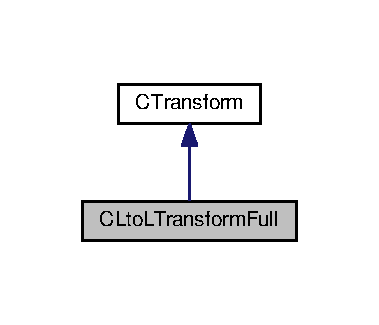
\includegraphics[width=182pt]{classCLtoLTransformFull__inherit__graph}
\end{center}
\end{figure}


Collaboration diagram for C\-Lto\-L\-Transform\-Full\-:\nopagebreak
\begin{figure}[H]
\begin{center}
\leavevmode
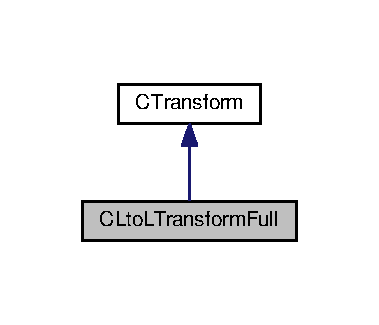
\includegraphics[width=182pt]{classCLtoLTransformFull__coll__graph}
\end{center}
\end{figure}
\subsection*{Public Member Functions}
\begin{DoxyCompactItemize}
\item 
\hyperlink{classCLtoLTransformFull_a592d0060608a21103a0fbbc1128210db}{C\-Lto\-L\-Transform\-Full} (const double $\ast$mat, int pm, int pn, double scale)
\item 
void \hyperlink{classCLtoLTransformFull_ad864ff448dcbf66777aeb968b00ad56e}{apply} (const \hyperlink{classCLocalExpan}{C\-Local\-Expan} \&Lin, \hyperlink{classCLocalExpan}{C\-Local\-Expan} \&Lout) const 
\item 
void \hyperlink{classCLtoLTransformFull_a94f06010f02e569eb05bea892ab0ac59}{apply} (const \hyperlink{classCTriExpan}{C\-Tri\-Expan} \&Ein, \hyperlink{classCTriExpan}{C\-Tri\-Expan} \&Eout) const 
\begin{DoxyCompactList}\small\item\em The \hyperlink{classCTransform}{C\-Transform} apply function. \end{DoxyCompactList}\end{DoxyCompactItemize}
\subsection*{Additional Inherited Members}


\subsection{Detailed Description}
The \hyperlink{classCLtoLTransformFull}{C\-Lto\-L\-Transform\-Full} class

Converts Full matrix local-\/to-\/local transform 

\subsection{Constructor \& Destructor Documentation}
\hypertarget{classCLtoLTransformFull_a592d0060608a21103a0fbbc1128210db}{\index{C\-Lto\-L\-Transform\-Full@{C\-Lto\-L\-Transform\-Full}!C\-Lto\-L\-Transform\-Full@{C\-Lto\-L\-Transform\-Full}}
\index{C\-Lto\-L\-Transform\-Full@{C\-Lto\-L\-Transform\-Full}!CLtoLTransformFull@{C\-Lto\-L\-Transform\-Full}}
\subsubsection[{C\-Lto\-L\-Transform\-Full}]{\setlength{\rightskip}{0pt plus 5cm}C\-Lto\-L\-Transform\-Full\-::\-C\-Lto\-L\-Transform\-Full (
\begin{DoxyParamCaption}
\item[{const double $\ast$}]{mat, }
\item[{int}]{pm, }
\item[{int}]{pn, }
\item[{double}]{scale}
\end{DoxyParamCaption}
)\hspace{0.3cm}{\ttfamily [inline]}}}\label{classCLtoLTransformFull_a592d0060608a21103a0fbbc1128210db}


\subsection{Member Function Documentation}
\hypertarget{classCLtoLTransformFull_ad864ff448dcbf66777aeb968b00ad56e}{\index{C\-Lto\-L\-Transform\-Full@{C\-Lto\-L\-Transform\-Full}!apply@{apply}}
\index{apply@{apply}!CLtoLTransformFull@{C\-Lto\-L\-Transform\-Full}}
\subsubsection[{apply}]{\setlength{\rightskip}{0pt plus 5cm}void C\-Lto\-L\-Transform\-Full\-::apply (
\begin{DoxyParamCaption}
\item[{const {\bf C\-Local\-Expan} \&}]{Lin, }
\item[{{\bf C\-Local\-Expan} \&}]{Lout}
\end{DoxyParamCaption}
) const\hspace{0.3cm}{\ttfamily [inline]}}}\label{classCLtoLTransformFull_ad864ff448dcbf66777aeb968b00ad56e}
\hypertarget{classCLtoLTransformFull_a94f06010f02e569eb05bea892ab0ac59}{\index{C\-Lto\-L\-Transform\-Full@{C\-Lto\-L\-Transform\-Full}!apply@{apply}}
\index{apply@{apply}!CLtoLTransformFull@{C\-Lto\-L\-Transform\-Full}}
\subsubsection[{apply}]{\setlength{\rightskip}{0pt plus 5cm}void C\-Lto\-L\-Transform\-Full\-::apply (
\begin{DoxyParamCaption}
\item[{const {\bf C\-Tri\-Expan} \&}]{Ein, }
\item[{{\bf C\-Tri\-Expan} \&}]{Eout}
\end{DoxyParamCaption}
) const\hspace{0.3cm}{\ttfamily [inline]}}}\label{classCLtoLTransformFull_a94f06010f02e569eb05bea892ab0ac59}


The \hyperlink{classCTransform}{C\-Transform} apply function. 

Applies a transform to a tricoeff object 

Reimplemented from \hyperlink{classCTransform_a986c0b58c44e47823f6811eeb4b5d096}{C\-Transform}.



Here is the call graph for this function\-:\nopagebreak
\begin{figure}[H]
\begin{center}
\leavevmode
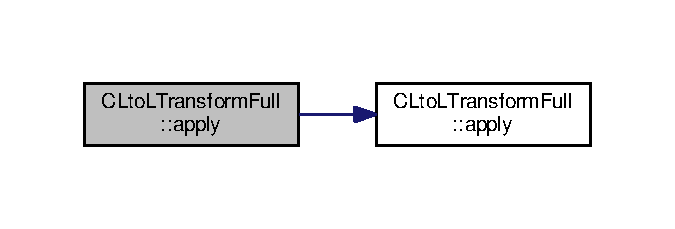
\includegraphics[width=324pt]{classCLtoLTransformFull_a94f06010f02e569eb05bea892ab0ac59_cgraph}
\end{center}
\end{figure}




The documentation for this class was generated from the following file\-:\begin{DoxyCompactItemize}
\item 
\hyperlink{transform_8h}{transform.\-h}\end{DoxyCompactItemize}

\hypertarget{classCLtoMTransformFull}{\section{C\-Lto\-M\-Transform\-Full Class Reference}
\label{classCLtoMTransformFull}\index{C\-Lto\-M\-Transform\-Full@{C\-Lto\-M\-Transform\-Full}}
}


{\ttfamily \#include $<$transform.\-h$>$}



Inheritance diagram for C\-Lto\-M\-Transform\-Full\-:\nopagebreak
\begin{figure}[H]
\begin{center}
\leavevmode
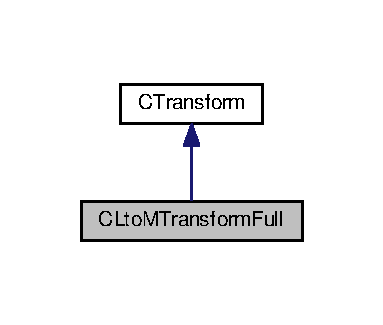
\includegraphics[width=184pt]{classCLtoMTransformFull__inherit__graph}
\end{center}
\end{figure}


Collaboration diagram for C\-Lto\-M\-Transform\-Full\-:\nopagebreak
\begin{figure}[H]
\begin{center}
\leavevmode
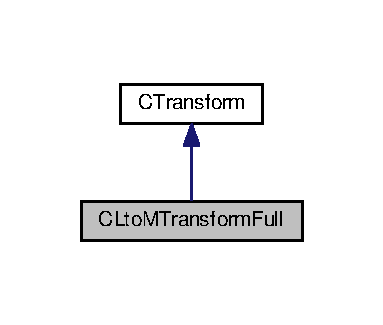
\includegraphics[width=184pt]{classCLtoMTransformFull__coll__graph}
\end{center}
\end{figure}
\subsection*{Public Member Functions}
\begin{DoxyCompactItemize}
\item 
\hyperlink{classCLtoMTransformFull_a6edc06029984f8eae5c4bac6f468afe1}{C\-Lto\-M\-Transform\-Full} (const double $\ast$mat, int pm, int pn, double scale)
\item 
void \hyperlink{classCLtoMTransformFull_a1262793a8fa9737e883db21560df7974}{apply} (const \hyperlink{classCLocalExpan}{C\-Local\-Expan} \&Lin, \hyperlink{classCMulExpan}{C\-Mul\-Expan} \&Mout) const 
\item 
void \hyperlink{classCLtoMTransformFull_a33fc7534a1f9a6db9f55353f12df96dd}{apply} (const \hyperlink{classCTriExpan}{C\-Tri\-Expan} \&Ein, \hyperlink{classCTriExpan}{C\-Tri\-Expan} \&Eout) const 
\begin{DoxyCompactList}\small\item\em The \hyperlink{classCTransform}{C\-Transform} apply function. \end{DoxyCompactList}\end{DoxyCompactItemize}
\subsection*{Additional Inherited Members}


\subsection{Detailed Description}
The \hyperlink{classCLtoMTransformFull}{C\-Lto\-M\-Transform\-Full} class

Converts local to multipole transform 

\subsection{Constructor \& Destructor Documentation}
\hypertarget{classCLtoMTransformFull_a6edc06029984f8eae5c4bac6f468afe1}{\index{C\-Lto\-M\-Transform\-Full@{C\-Lto\-M\-Transform\-Full}!C\-Lto\-M\-Transform\-Full@{C\-Lto\-M\-Transform\-Full}}
\index{C\-Lto\-M\-Transform\-Full@{C\-Lto\-M\-Transform\-Full}!CLtoMTransformFull@{C\-Lto\-M\-Transform\-Full}}
\subsubsection[{C\-Lto\-M\-Transform\-Full}]{\setlength{\rightskip}{0pt plus 5cm}C\-Lto\-M\-Transform\-Full\-::\-C\-Lto\-M\-Transform\-Full (
\begin{DoxyParamCaption}
\item[{const double $\ast$}]{mat, }
\item[{int}]{pm, }
\item[{int}]{pn, }
\item[{double}]{scale}
\end{DoxyParamCaption}
)\hspace{0.3cm}{\ttfamily [inline]}}}\label{classCLtoMTransformFull_a6edc06029984f8eae5c4bac6f468afe1}


\subsection{Member Function Documentation}
\hypertarget{classCLtoMTransformFull_a1262793a8fa9737e883db21560df7974}{\index{C\-Lto\-M\-Transform\-Full@{C\-Lto\-M\-Transform\-Full}!apply@{apply}}
\index{apply@{apply}!CLtoMTransformFull@{C\-Lto\-M\-Transform\-Full}}
\subsubsection[{apply}]{\setlength{\rightskip}{0pt plus 5cm}void C\-Lto\-M\-Transform\-Full\-::apply (
\begin{DoxyParamCaption}
\item[{const {\bf C\-Local\-Expan} \&}]{Lin, }
\item[{{\bf C\-Mul\-Expan} \&}]{Mout}
\end{DoxyParamCaption}
) const\hspace{0.3cm}{\ttfamily [inline]}}}\label{classCLtoMTransformFull_a1262793a8fa9737e883db21560df7974}
\hypertarget{classCLtoMTransformFull_a33fc7534a1f9a6db9f55353f12df96dd}{\index{C\-Lto\-M\-Transform\-Full@{C\-Lto\-M\-Transform\-Full}!apply@{apply}}
\index{apply@{apply}!CLtoMTransformFull@{C\-Lto\-M\-Transform\-Full}}
\subsubsection[{apply}]{\setlength{\rightskip}{0pt plus 5cm}void C\-Lto\-M\-Transform\-Full\-::apply (
\begin{DoxyParamCaption}
\item[{const {\bf C\-Tri\-Expan} \&}]{Ein, }
\item[{{\bf C\-Tri\-Expan} \&}]{Eout}
\end{DoxyParamCaption}
) const\hspace{0.3cm}{\ttfamily [inline]}}}\label{classCLtoMTransformFull_a33fc7534a1f9a6db9f55353f12df96dd}


The \hyperlink{classCTransform}{C\-Transform} apply function. 

Applies a transform to a tricoeff object 

Reimplemented from \hyperlink{classCTransform_a986c0b58c44e47823f6811eeb4b5d096}{C\-Transform}.



Here is the call graph for this function\-:\nopagebreak
\begin{figure}[H]
\begin{center}
\leavevmode
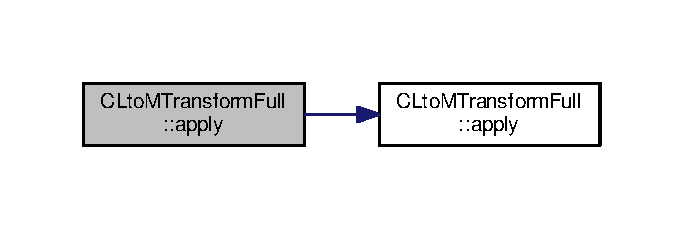
\includegraphics[width=328pt]{classCLtoMTransformFull_a33fc7534a1f9a6db9f55353f12df96dd_cgraph}
\end{center}
\end{figure}




The documentation for this class was generated from the following file\-:\begin{DoxyCompactItemize}
\item 
\hyperlink{transform_8h}{transform.\-h}\end{DoxyCompactItemize}

\hypertarget{classCMExpan}{\section{C\-M\-Expan Class Reference}
\label{classCMExpan}\index{C\-M\-Expan@{C\-M\-Expan}}
}


{\ttfamily \#include $<$expansion.\-h$>$}



Inheritance diagram for C\-M\-Expan\-:\nopagebreak
\begin{figure}[H]
\begin{center}
\leavevmode
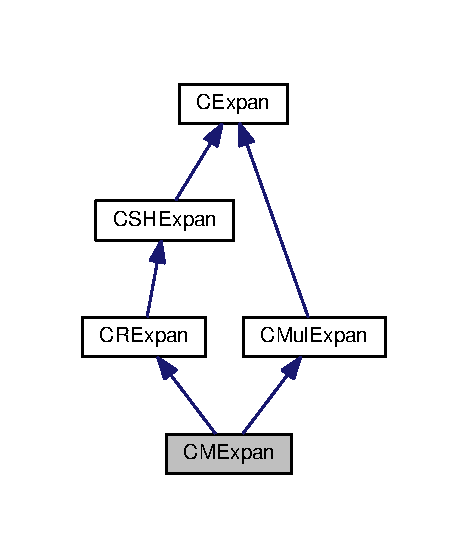
\includegraphics[width=225pt]{classCMExpan__inherit__graph}
\end{center}
\end{figure}


Collaboration diagram for C\-M\-Expan\-:\nopagebreak
\begin{figure}[H]
\begin{center}
\leavevmode
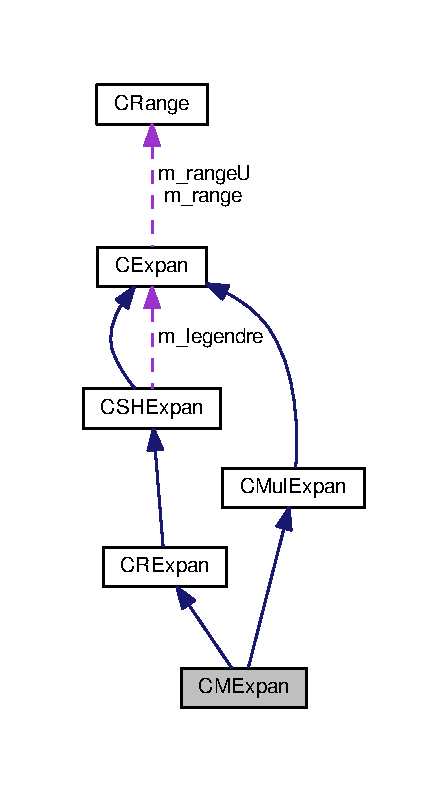
\includegraphics[width=215pt]{classCMExpan__coll__graph}
\end{center}
\end{figure}
\subsection*{Public Member Functions}
\begin{DoxyCompactItemize}
\item 
\hyperlink{classCMExpan_afc2ced05f674474dee519627ca6f46ee}{C\-M\-Expan} (\hyperlink{util_8h_a5821460e95a0800cf9f24c38915cbbde}{R\-E\-A\-L} ch, const \hyperlink{classCSpPnt}{C\-Sp\-Pnt} \&spos, bool b\-Kappa, int p, double scale=1.\-0)
\begin{DoxyCompactList}\small\item\em \hyperlink{classCMExpan}{C\-M\-Expan} class constructor. \end{DoxyCompactList}\item 
\hyperlink{classCMExpan_ab7ef3ccf42356939efa9936eff3ad2b7}{C\-M\-Expan} (const \hyperlink{classCMExpan}{C\-M\-Expan} \&M)
\item 
virtual void \hyperlink{classCMExpan_a699048991f3a09ed9b7991e33ad422d7}{init} ()
\begin{DoxyCompactList}\small\item\em \hyperlink{classCMExpan}{C\-M\-Expan} init function. \end{DoxyCompactList}\item 
const \hyperlink{classCMExpan}{C\-M\-Expan} \& \hyperlink{classCMExpan_a8c16ac85626b9bdbbe3953ca2c285158}{operator=} (const \hyperlink{classCMExpan}{C\-M\-Expan} \&M)
\item 
virtual \hyperlink{classCExpan}{C\-Expan} \hyperlink{classCMExpan_af9582edc26146339150b209b7cdd2f0e}{d\-Mdr} () const 
\end{DoxyCompactItemize}


Collaboration diagram for C\-Mto\-L\-Transform\-Full\-:\nopagebreak
\begin{figure}[H]
\begin{center}
\leavevmode
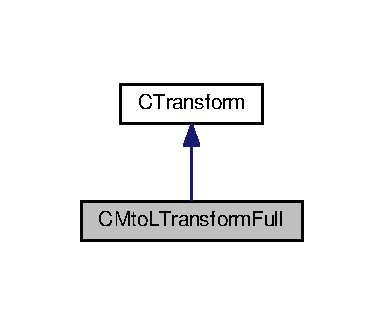
\includegraphics[width=184pt]{classCMtoLTransformFull__coll__graph}
\end{center}
\end{figure}
\subsection*{Public Member Functions}
\begin{DoxyCompactItemize}
\item 
\hyperlink{classCMtoLTransformFull_ad215fa519e66560c6b02a855ea027a14}{C\-Mto\-L\-Transform\-Full} (const double $\ast$mat, int pm, int pn, double scale)
\item 
void \hyperlink{classCMtoLTransformFull_ad5b9982a8350902b84a36426e910cee0}{apply} (const \hyperlink{classCMulExpan}{C\-Mul\-Expan} \&Min, \hyperlink{classCLocalExpan}{C\-Local\-Expan} \&Lout) const 
\end{DoxyCompactItemize}
\subsection*{Additional Inherited Members}


\subsection{Detailed Description}
The \hyperlink{classCMtoLTransformFull}{C\-Mto\-L\-Transform\-Full} class

Converts multipole to local transform 

\subsection{Constructor \& Destructor Documentation}
\hypertarget{classCMtoLTransformFull_ad215fa519e66560c6b02a855ea027a14}{\index{C\-Mto\-L\-Transform\-Full@{C\-Mto\-L\-Transform\-Full}!C\-Mto\-L\-Transform\-Full@{C\-Mto\-L\-Transform\-Full}}
\index{C\-Mto\-L\-Transform\-Full@{C\-Mto\-L\-Transform\-Full}!CMtoLTransformFull@{C\-Mto\-L\-Transform\-Full}}
\subsubsection[{C\-Mto\-L\-Transform\-Full}]{\setlength{\rightskip}{0pt plus 5cm}C\-Mto\-L\-Transform\-Full\-::\-C\-Mto\-L\-Transform\-Full (
\begin{DoxyParamCaption}
\item[{const double $\ast$}]{mat, }
\item[{int}]{pm, }
\item[{int}]{pn, }
\item[{double}]{scale}
\end{DoxyParamCaption}
)\hspace{0.3cm}{\ttfamily [inline]}}}\label{classCMtoLTransformFull_ad215fa519e66560c6b02a855ea027a14}


\subsection{Member Function Documentation}
\hypertarget{classCMtoLTransformFull_ad5b9982a8350902b84a36426e910cee0}{\index{C\-Mto\-L\-Transform\-Full@{C\-Mto\-L\-Transform\-Full}!apply@{apply}}
\index{apply@{apply}!CMtoLTransformFull@{C\-Mto\-L\-Transform\-Full}}
\subsubsection[{apply}]{\setlength{\rightskip}{0pt plus 5cm}void C\-Mto\-L\-Transform\-Full\-::apply (
\begin{DoxyParamCaption}
\item[{const {\bf C\-Mul\-Expan} \&}]{Min, }
\item[{{\bf C\-Local\-Expan} \&}]{Lout}
\end{DoxyParamCaption}
) const\hspace{0.3cm}{\ttfamily [inline]}}}\label{classCMtoLTransformFull_ad5b9982a8350902b84a36426e910cee0}


The documentation for this class was generated from the following file\-:\begin{DoxyCompactItemize}
\item 
\hyperlink{transform_8h}{transform.\-h}\end{DoxyCompactItemize}

\input{classCMolCell}
\input{classCMolContact}
\input{classCMolContactRigid}
\input{classCMolecule}
\input{classCMtoLTransformFull}
\hypertarget{classCMtoMTransformFull}{\section{C\-Mto\-M\-Transform\-Full Class Reference}
\label{classCMtoMTransformFull}\index{C\-Mto\-M\-Transform\-Full@{C\-Mto\-M\-Transform\-Full}}
}


{\ttfamily \#include $<$transform.\-h$>$}



Inheritance diagram for C\-Mto\-M\-Transform\-Full\-:\nopagebreak
\begin{figure}[H]
\begin{center}
\leavevmode
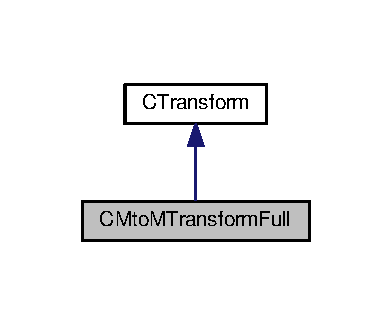
\includegraphics[width=188pt]{classCMtoMTransformFull__inherit__graph}
\end{center}
\end{figure}


Collaboration diagram for C\-Mto\-M\-Transform\-Full\-:\nopagebreak
\begin{figure}[H]
\begin{center}
\leavevmode
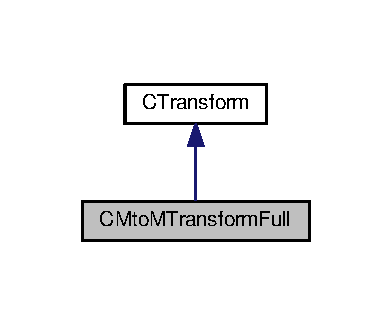
\includegraphics[width=188pt]{classCMtoMTransformFull__coll__graph}
\end{center}
\end{figure}
\subsection*{Public Member Functions}
\begin{DoxyCompactItemize}
\item 
\hyperlink{classCMtoMTransformFull_a153149877b790867c17e7a1ad7d64747}{C\-Mto\-M\-Transform\-Full} (const double $\ast$mat, int pm, int pn, double scale)
\item 
void \hyperlink{classCMtoMTransformFull_a188edd638a34bc0228eb8197145c288a}{apply} (const \hyperlink{classCMulExpan}{C\-Mul\-Expan} \&Min, \hyperlink{classCMulExpan}{C\-Mul\-Expan} \&Mout) const 
\end{DoxyCompactItemize}
\subsection*{Additional Inherited Members}


\subsection{Detailed Description}
The \hyperlink{classCMtoMTransformFull}{C\-Mto\-M\-Transform\-Full} class

Converts Full matrix multipole-\/to-\/multipole transform 

\subsection{Constructor \& Destructor Documentation}
\hypertarget{classCMtoMTransformFull_a153149877b790867c17e7a1ad7d64747}{\index{C\-Mto\-M\-Transform\-Full@{C\-Mto\-M\-Transform\-Full}!C\-Mto\-M\-Transform\-Full@{C\-Mto\-M\-Transform\-Full}}
\index{C\-Mto\-M\-Transform\-Full@{C\-Mto\-M\-Transform\-Full}!CMtoMTransformFull@{C\-Mto\-M\-Transform\-Full}}
\subsubsection[{C\-Mto\-M\-Transform\-Full}]{\setlength{\rightskip}{0pt plus 5cm}C\-Mto\-M\-Transform\-Full\-::\-C\-Mto\-M\-Transform\-Full (
\begin{DoxyParamCaption}
\item[{const double $\ast$}]{mat, }
\item[{int}]{pm, }
\item[{int}]{pn, }
\item[{double}]{scale}
\end{DoxyParamCaption}
)\hspace{0.3cm}{\ttfamily [inline]}}}\label{classCMtoMTransformFull_a153149877b790867c17e7a1ad7d64747}


\subsection{Member Function Documentation}
\hypertarget{classCMtoMTransformFull_a188edd638a34bc0228eb8197145c288a}{\index{C\-Mto\-M\-Transform\-Full@{C\-Mto\-M\-Transform\-Full}!apply@{apply}}
\index{apply@{apply}!CMtoMTransformFull@{C\-Mto\-M\-Transform\-Full}}
\subsubsection[{apply}]{\setlength{\rightskip}{0pt plus 5cm}void C\-Mto\-M\-Transform\-Full\-::apply (
\begin{DoxyParamCaption}
\item[{const {\bf C\-Mul\-Expan} \&}]{Min, }
\item[{{\bf C\-Mul\-Expan} \&}]{Mout}
\end{DoxyParamCaption}
) const\hspace{0.3cm}{\ttfamily [inline]}}}\label{classCMtoMTransformFull_a188edd638a34bc0228eb8197145c288a}


The documentation for this class was generated from the following file\-:\begin{DoxyCompactItemize}
\item 
\hyperlink{transform_8h}{transform.\-h}\end{DoxyCompactItemize}

\hypertarget{classCMulExpan}{\section{C\-Mul\-Expan Class Reference}
\label{classCMulExpan}\index{C\-Mul\-Expan@{C\-Mul\-Expan}}
}


{\ttfamily \#include $<$expansion.\-h$>$}



Inheritance diagram for C\-Mul\-Expan\-:\nopagebreak
\begin{figure}[H]
\begin{center}
\leavevmode
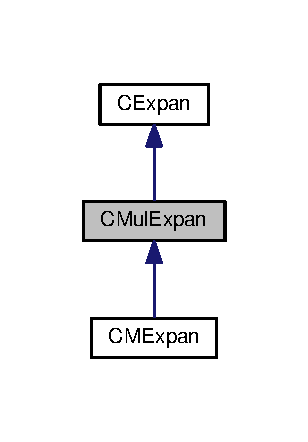
\includegraphics[width=148pt]{classCMulExpan__inherit__graph}
\end{center}
\end{figure}


Collaboration diagram for C\-Mul\-Expan\-:\nopagebreak
\begin{figure}[H]
\begin{center}
\leavevmode
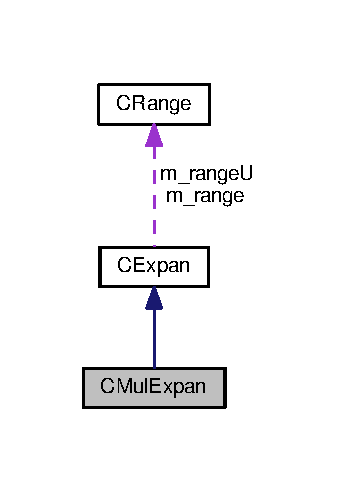
\includegraphics[width=163pt]{classCMulExpan__coll__graph}
\end{center}
\end{figure}
\subsection*{Public Member Functions}
\begin{DoxyCompactItemize}
\item 
\hyperlink{classCMulExpan_abcef941fb90e2e5c3e220d43396dfc37}{C\-Mul\-Expan} (const double $\ast$v, const \hyperlink{classCRange}{C\-Range} \&range, double scale=1.\-0)
\begin{DoxyCompactList}\small\item\em The \hyperlink{classCMulExpan}{C\-Mul\-Expan} class constructor. \end{DoxyCompactList}\item 
\hyperlink{classCMulExpan_a931ae750321cb051d5d374854bc8a424}{C\-Mul\-Expan} (const vector$<$ \hyperlink{util_8h_a5821460e95a0800cf9f24c38915cbbde}{R\-E\-A\-L} $>$ M, const \hyperlink{classCRange}{C\-Range} \&range, double scale=1.\-0)
\item 
\hyperlink{classCMulExpan_a4256da905269df8c3f78230b69e8e3e1}{C\-Mul\-Expan} (const vector$<$ \hyperlink{util_8h_a5821460e95a0800cf9f24c38915cbbde}{R\-E\-A\-L} $>$ \&ch, const vector$<$ \hyperlink{classCPnt}{C\-Pnt} $>$ \&pos, int p, bool b\-Kappa, \hyperlink{util_8h_a5821460e95a0800cf9f24c38915cbbde}{R\-E\-A\-L} scale)
\begin{DoxyCompactList}\small\item\em The \hyperlink{classCMulExpan}{C\-Mul\-Expan} class constructor. \end{DoxyCompactList}\item 
\hyperlink{classCMulExpan_ae557c77c098763a39a0c5ad266517304}{C\-Mul\-Expan} (int p=0)
\item 
\hyperlink{classCMulExpan_a95beaf89b77d13f7525562138d0ac2df}{C\-Mul\-Expan} (const \hyperlink{classCRange}{C\-Range} \&range, \hyperlink{util_8h_a5821460e95a0800cf9f24c38915cbbde}{R\-E\-A\-L} scale=1.\-0)
\end{DoxyCompactItemize}
\subsection*{Friends}
\begin{DoxyCompactItemize}
\item 
\hyperlink{util_8h_a5821460e95a0800cf9f24c38915cbbde}{R\-E\-A\-L} \hyperlink{classCMulExpan_a020c55be9514911fc8ecde0a8d81a919}{inprod} (const \hyperlink{classCMulExpan}{C\-Mul\-Expan} \&M, const \hyperlink{classCLocalExpan}{C\-Local\-Expan} \&L)
\end{DoxyCompactItemize}
\subsection*{Additional Inherited Members}


\subsection{Detailed Description}
The \hyperlink{classCMulExpan}{C\-Mul\-Expan} class

The \hyperlink{classCMulExpan}{C\-Mul\-Expan} class contains information about general multipole expansion class. 

\subsection{Constructor \& Destructor Documentation}
\hypertarget{classCMulExpan_abcef941fb90e2e5c3e220d43396dfc37}{\index{C\-Mul\-Expan@{C\-Mul\-Expan}!C\-Mul\-Expan@{C\-Mul\-Expan}}
\index{C\-Mul\-Expan@{C\-Mul\-Expan}!CMulExpan@{C\-Mul\-Expan}}
\subsubsection[{C\-Mul\-Expan}]{\setlength{\rightskip}{0pt plus 5cm}C\-Mul\-Expan\-::\-C\-Mul\-Expan (
\begin{DoxyParamCaption}
\item[{const double $\ast$}]{v, }
\item[{const {\bf C\-Range} \&}]{range, }
\item[{double}]{scale = {\ttfamily 1.0}}
\end{DoxyParamCaption}
)\hspace{0.3cm}{\ttfamily [inline]}}}\label{classCMulExpan_abcef941fb90e2e5c3e220d43396dfc37}


The \hyperlink{classCMulExpan}{C\-Mul\-Expan} class constructor. 

Initialize a \hyperlink{classCMulExpan}{C\-Mul\-Expan} object from a vector of coefficients. 
\begin{DoxyParams}{Parameters}
{\em p} & is an int that is a minimal number of poles. Default is zero. \\
\hline
{\em range} & a \hyperlink{classCRange}{C\-Range} object of the range of \\
\hline
\end{DoxyParams}
\hypertarget{classCMulExpan_a931ae750321cb051d5d374854bc8a424}{\index{C\-Mul\-Expan@{C\-Mul\-Expan}!C\-Mul\-Expan@{C\-Mul\-Expan}}
\index{C\-Mul\-Expan@{C\-Mul\-Expan}!CMulExpan@{C\-Mul\-Expan}}
\subsubsection[{C\-Mul\-Expan}]{\setlength{\rightskip}{0pt plus 5cm}C\-Mul\-Expan\-::\-C\-Mul\-Expan (
\begin{DoxyParamCaption}
\item[{const vector$<$ {\bf R\-E\-A\-L} $>$}]{M, }
\item[{const {\bf C\-Range} \&}]{range, }
\item[{double}]{scale = {\ttfamily 1.0}}
\end{DoxyParamCaption}
)\hspace{0.3cm}{\ttfamily [inline]}}}\label{classCMulExpan_a931ae750321cb051d5d374854bc8a424}
\hypertarget{classCMulExpan_a4256da905269df8c3f78230b69e8e3e1}{\index{C\-Mul\-Expan@{C\-Mul\-Expan}!C\-Mul\-Expan@{C\-Mul\-Expan}}
\index{C\-Mul\-Expan@{C\-Mul\-Expan}!CMulExpan@{C\-Mul\-Expan}}
\subsubsection[{C\-Mul\-Expan}]{\setlength{\rightskip}{0pt plus 5cm}C\-Mul\-Expan\-::\-C\-Mul\-Expan (
\begin{DoxyParamCaption}
\item[{const vector$<$ {\bf R\-E\-A\-L} $>$ \&}]{ch, }
\item[{const vector$<$ {\bf C\-Pnt} $>$ \&}]{pos, }
\item[{int}]{p, }
\item[{bool}]{b\-Kappa, }
\item[{{\bf R\-E\-A\-L}}]{scale}
\end{DoxyParamCaption}
)}}\label{classCMulExpan_a4256da905269df8c3f78230b69e8e3e1}


The \hyperlink{classCMulExpan}{C\-Mul\-Expan} class constructor. 

Initialize a \hyperlink{classCMulExpan}{C\-Mul\-Expan} object of a set of charges, creates an M\-Expan object. 
\begin{DoxyParams}{Parameters}
{\em ch} & a vector of point charges \\
\hline
{\em pos} & a vector of point charge X\-Y\-Z coordinates \\
\hline
{\em p} & is an int that is the number of poles. \\
\hline
{\em b\-Kappa} & a boolean of whether of not to include screened charges \\
\hline
{\em scale} & a length scale for the expansion\\
\hline
\end{DoxyParams}
Construct a multipole expansion for a set of charges, calls M\-Expan constructor 

Here is the call graph for this function\-:\nopagebreak
\begin{figure}[H]
\begin{center}
\leavevmode
\includegraphics[width=350pt]{classCMulExpan_a4256da905269df8c3f78230b69e8e3e1_cgraph}
\end{center}
\end{figure}


\hypertarget{classCMulExpan_ae557c77c098763a39a0c5ad266517304}{\index{C\-Mul\-Expan@{C\-Mul\-Expan}!C\-Mul\-Expan@{C\-Mul\-Expan}}
\index{C\-Mul\-Expan@{C\-Mul\-Expan}!CMulExpan@{C\-Mul\-Expan}}
\subsubsection[{C\-Mul\-Expan}]{\setlength{\rightskip}{0pt plus 5cm}C\-Mul\-Expan\-::\-C\-Mul\-Expan (
\begin{DoxyParamCaption}
\item[{int}]{p = {\ttfamily 0}}
\end{DoxyParamCaption}
)\hspace{0.3cm}{\ttfamily [inline]}}}\label{classCMulExpan_ae557c77c098763a39a0c5ad266517304}
\hypertarget{classCMulExpan_a95beaf89b77d13f7525562138d0ac2df}{\index{C\-Mul\-Expan@{C\-Mul\-Expan}!C\-Mul\-Expan@{C\-Mul\-Expan}}
\index{C\-Mul\-Expan@{C\-Mul\-Expan}!CMulExpan@{C\-Mul\-Expan}}
\subsubsection[{C\-Mul\-Expan}]{\setlength{\rightskip}{0pt plus 5cm}C\-Mul\-Expan\-::\-C\-Mul\-Expan (
\begin{DoxyParamCaption}
\item[{const {\bf C\-Range} \&}]{range, }
\item[{{\bf R\-E\-A\-L}}]{scale = {\ttfamily 1.0}}
\end{DoxyParamCaption}
)\hspace{0.3cm}{\ttfamily [inline]}}}\label{classCMulExpan_a95beaf89b77d13f7525562138d0ac2df}


\subsection{Friends And Related Function Documentation}
\hypertarget{classCMulExpan_a020c55be9514911fc8ecde0a8d81a919}{\index{C\-Mul\-Expan@{C\-Mul\-Expan}!inprod@{inprod}}
\index{inprod@{inprod}!CMulExpan@{C\-Mul\-Expan}}
\subsubsection[{inprod}]{\setlength{\rightskip}{0pt plus 5cm}{\bf R\-E\-A\-L} inprod (
\begin{DoxyParamCaption}
\item[{const {\bf C\-Mul\-Expan} \&}]{M, }
\item[{const {\bf C\-Local\-Expan} \&}]{L}
\end{DoxyParamCaption}
)\hspace{0.3cm}{\ttfamily [friend]}}}\label{classCMulExpan_a020c55be9514911fc8ecde0a8d81a919}


The documentation for this class was generated from the following files\-:\begin{DoxyCompactItemize}
\item 
\hyperlink{expansion_8h}{expansion.\-h}\item 
\hyperlink{expansion_8cpp}{expansion.\-cpp}\end{DoxyCompactItemize}

\hypertarget{classCPnt}{\section{C\-Pnt Class Reference}
\label{classCPnt}\index{C\-Pnt@{C\-Pnt}}
}


The \hyperlink{classCPnt}{C\-Pnt} class.  




{\ttfamily \#include $<$util.\-h$>$}

\subsection*{Public Member Functions}
\begin{DoxyCompactItemize}
\item 
\hyperlink{classCPnt_a6792dcfc8b95c18c03bda5a6dde7765a}{C\-Pnt} ()
\begin{DoxyCompactList}\small\item\em The \hyperlink{classCPnt}{C\-Pnt} class constructor. \end{DoxyCompactList}\item 
\hyperlink{classCPnt_a91907d073421cdf75000d27f982f058b}{C\-Pnt} (\hyperlink{util_8h_a5821460e95a0800cf9f24c38915cbbde}{R\-E\-A\-L} x\-\_\-, \hyperlink{util_8h_a5821460e95a0800cf9f24c38915cbbde}{R\-E\-A\-L} y\-\_\-, \hyperlink{util_8h_a5821460e95a0800cf9f24c38915cbbde}{R\-E\-A\-L} z\-\_\-)
\begin{DoxyCompactList}\small\item\em The \hyperlink{classCPnt}{C\-Pnt} class constructor. \end{DoxyCompactList}\item 
\hyperlink{classCPnt_aca4d8d7044e71700128b497cfcc4f1d8}{C\-Pnt} (const \hyperlink{classCPnt}{C\-Pnt} \&p)
\begin{DoxyCompactList}\small\item\em The \hyperlink{classCPnt}{C\-Pnt} class constructor. \end{DoxyCompactList}\item 
const \hyperlink{classCPnt}{C\-Pnt} \& \hyperlink{classCPnt_abd18aa7c83ac70f5e73847a8cd154e9d}{operator=} (const \hyperlink{classCPnt}{C\-Pnt} \&c)
\begin{DoxyCompactList}\small\item\em The \hyperlink{classCPnt}{C\-Pnt} class = operator. \end{DoxyCompactList}\item 
void \hyperlink{classCPnt_a619a71665a5a40fddbc8e6c6a6b450cc}{zero} ()
\begin{DoxyCompactList}\small\item\em The \hyperlink{classCPnt}{C\-Pnt} class zero function. \end{DoxyCompactList}\item 
\hyperlink{util_8h_a5821460e95a0800cf9f24c38915cbbde}{R\-E\-A\-L} \hyperlink{classCPnt_ac4dcf209c35c4ef0c119cd59fbddd18f}{normsq} () const 
\begin{DoxyCompactList}\small\item\em The \hyperlink{classCSpPnt}{C\-Sp\-Pnt} class normsq function. \end{DoxyCompactList}\item 
\hyperlink{util_8h_a5821460e95a0800cf9f24c38915cbbde}{R\-E\-A\-L} \hyperlink{classCPnt_ab92f2e6cc3891ff6a00eddb483b854ab}{norm} () const 
\begin{DoxyCompactList}\small\item\em The \hyperlink{classCPnt}{C\-Pnt} norm function. \end{DoxyCompactList}\item 
const \hyperlink{classCPnt}{C\-Pnt} \& \hyperlink{classCPnt_a79e4515e6479905942ce4b48990943f0}{normalize} ()
\begin{DoxyCompactList}\small\item\em The \hyperlink{classCPnt}{C\-Pnt} normalize function. \end{DoxyCompactList}\item 
\hyperlink{classCPnt}{C\-Pnt} \hyperlink{classCPnt_a59899074de56c4ad55583fc58d48ea0a}{normalize} () const 
\begin{DoxyCompactList}\small\item\em The \hyperlink{classCPnt}{C\-Pnt} normalize function. \end{DoxyCompactList}\item 
void \hyperlink{classCPnt_ab9aa57d527e60e0ba46fd44ee515ebb0}{operator+=} (const \hyperlink{classCPnt}{C\-Pnt} \&p)
\item 
void \hyperlink{classCPnt_aad46f39ec4811f1f7c39b33b0ef55f42}{operator-\/=} (const \hyperlink{classCPnt}{C\-Pnt} \&p)
\item 
void \hyperlink{classCPnt_a30b6c20eb5777d321202db9006fe5dc0}{operator$\ast$=} (\hyperlink{util_8h_a5821460e95a0800cf9f24c38915cbbde}{R\-E\-A\-L} s)
\item 
void \hyperlink{classCPnt_a5ef5437f322871129c1398ab5f5e8764}{operator/=} (\hyperlink{util_8h_a5821460e95a0800cf9f24c38915cbbde}{R\-E\-A\-L} s)
\item 
const \hyperlink{util_8h_a5821460e95a0800cf9f24c38915cbbde}{R\-E\-A\-L} \hyperlink{classCPnt_a5867d45fc05ae371116367067eb23f48}{x} () const 
\begin{DoxyCompactList}\small\item\em The \hyperlink{classCSpPnt}{C\-Sp\-Pnt} class print x. \end{DoxyCompactList}\item 
const \hyperlink{util_8h_a5821460e95a0800cf9f24c38915cbbde}{R\-E\-A\-L} \hyperlink{classCPnt_ac9283f60e70f312ee1784de6c6ea5aec}{y} () const 
\begin{DoxyCompactList}\small\item\em The \hyperlink{classCSpPnt}{C\-Sp\-Pnt} class print y. \end{DoxyCompactList}\item 
const \hyperlink{util_8h_a5821460e95a0800cf9f24c38915cbbde}{R\-E\-A\-L} \hyperlink{classCPnt_a37d139ebe50234ab753472b896c7d17c}{z} () const 
\begin{DoxyCompactList}\small\item\em The \hyperlink{classCSpPnt}{C\-Sp\-Pnt} class print z. \end{DoxyCompactList}\item 
\hyperlink{util_8h_a5821460e95a0800cf9f24c38915cbbde}{R\-E\-A\-L} \& \hyperlink{classCPnt_ac7a36844c1474f7d89f27c5ab3e083b2}{x} ()
\begin{DoxyCompactList}\small\item\em The \hyperlink{classCSpPnt}{C\-Sp\-Pnt} class print x. \end{DoxyCompactList}\item 
\hyperlink{util_8h_a5821460e95a0800cf9f24c38915cbbde}{R\-E\-A\-L} \& \hyperlink{classCPnt_afa7c12f6ae5daf81779e92692c5024ce}{y} ()
\begin{DoxyCompactList}\small\item\em The \hyperlink{classCSpPnt}{C\-Sp\-Pnt} class print y. \end{DoxyCompactList}\item 
\hyperlink{util_8h_a5821460e95a0800cf9f24c38915cbbde}{R\-E\-A\-L} \& \hyperlink{classCPnt_a6a5263d7b30cc4776336ac9598416757}{z} ()
\begin{DoxyCompactList}\small\item\em The \hyperlink{classCSpPnt}{C\-Sp\-Pnt} class print z. \end{DoxyCompactList}\end{DoxyCompactItemize}
\subsection*{Friends}
\begin{DoxyCompactItemize}
\item 
\hyperlink{classCPnt}{C\-Pnt} \hyperlink{classCPnt_a793e034bed9900c45412db255d708e84}{operator+} (const \hyperlink{classCPnt}{C\-Pnt} \&p1, const \hyperlink{classCPnt}{C\-Pnt} \&p2)
\begin{DoxyCompactList}\small\item\em \hyperlink{classCPnt}{C\-Pnt} +. \end{DoxyCompactList}\item 
\hyperlink{classCPnt}{C\-Pnt} \hyperlink{classCPnt_a7b0ef59814c5c3ae6a9165df62ab8598}{operator-\/} (const \hyperlink{classCPnt}{C\-Pnt} \&p1, const \hyperlink{classCPnt}{C\-Pnt} \&p2)
\begin{DoxyCompactList}\small\item\em \hyperlink{classCPnt}{C\-Pnt} -\/. \end{DoxyCompactList}\item 
\hyperlink{classCPnt}{C\-Pnt} \hyperlink{classCPnt_ab4553c75d2ac17d0539471baeb0c0237}{cross} (const \hyperlink{classCPnt}{C\-Pnt} \&p1, const \hyperlink{classCPnt}{C\-Pnt} \&p2)
\begin{DoxyCompactList}\small\item\em \hyperlink{classCPnt}{C\-Pnt} cross. \end{DoxyCompactList}\item 
\hyperlink{classCPnt}{C\-Pnt} \hyperlink{classCPnt_a6bf4a1152989f36cdb084e617a81214b}{operator$\ast$} (\hyperlink{util_8h_a5821460e95a0800cf9f24c38915cbbde}{R\-E\-A\-L} c, const \hyperlink{classCPnt}{C\-Pnt} \&p1)
\begin{DoxyCompactList}\small\item\em \hyperlink{classCPnt}{C\-Pnt} $\ast$ scalar. \end{DoxyCompactList}\item 
\hyperlink{classCPnt}{C\-Pnt} \hyperlink{classCPnt_a77ba614aeb115f5ab29247677cc4fa05}{operator-\/} (const \hyperlink{classCPnt}{C\-Pnt} \&p)
\begin{DoxyCompactList}\small\item\em \hyperlink{classCPnt}{C\-Pnt} -\/. \end{DoxyCompactList}\item 
ostream \& \hyperlink{classCPnt_a5d9fde839f5480f04e4b64a9621e3370}{operator$<$$<$} (ostream \&out, const \hyperlink{classCPnt}{C\-Pnt} \&p)
\begin{DoxyCompactList}\small\item\em \hyperlink{classCPnt}{C\-Pnt} $<$$<$. \end{DoxyCompactList}\item 
\hyperlink{classCPnt}{C\-Pnt} \hyperlink{classCPnt_af8b263bb80bb3a76271a7f57d5057df3}{Sph\-To\-Cart} (const \hyperlink{classCSpPnt}{C\-Sp\-Pnt} \&s)
\begin{DoxyCompactList}\small\item\em \hyperlink{classCSpPnt}{C\-Sp\-Pnt} Sph\-To\-Cart. \end{DoxyCompactList}\item 
\hyperlink{classCSpPnt}{C\-Sp\-Pnt} \hyperlink{classCPnt_ad05fbf75e7550a927bc817f97115f2fc}{Cart\-To\-Sph} (const \hyperlink{classCPnt}{C\-Pnt} \&c)
\begin{DoxyCompactList}\small\item\em \hyperlink{classCSpPnt}{C\-Sp\-Pnt} Cart\-To\-Sph. \end{DoxyCompactList}\item 
\hyperlink{util_8h_a5821460e95a0800cf9f24c38915cbbde}{R\-E\-A\-L} \hyperlink{classCPnt_ac25278586b4a84caf4098513d812d60b}{torsion} (const \hyperlink{classCPnt}{C\-Pnt} \&p1, const \hyperlink{classCPnt}{C\-Pnt} \&p2, const \hyperlink{classCPnt}{C\-Pnt} \&p3, const \hyperlink{classCPnt}{C\-Pnt} \&p4)
\begin{DoxyCompactList}\small\item\em \hyperlink{classCPnt}{C\-Pnt} torsion. \end{DoxyCompactList}\item 
\hyperlink{util_8h_a5821460e95a0800cf9f24c38915cbbde}{R\-E\-A\-L} \hyperlink{classCPnt_a774fe41d28888a078993d8d3384c34d8}{torsion} (const \hyperlink{classCPnt}{C\-Pnt} \&v1, const \hyperlink{classCPnt}{C\-Pnt} \&v2, const \hyperlink{classCPnt}{C\-Pnt} \&v3)
\begin{DoxyCompactList}\small\item\em \hyperlink{classCPnt}{C\-Pnt} torsion. \end{DoxyCompactList}\end{DoxyCompactItemize}


\subsection{Detailed Description}
The \hyperlink{classCPnt}{C\-Pnt} class. 

The cartesian coordinate class. Contains a set of cartesian coordinates and operations that may be performed on it. 

\subsection{Constructor \& Destructor Documentation}
\hypertarget{classCPnt_a6792dcfc8b95c18c03bda5a6dde7765a}{\index{C\-Pnt@{C\-Pnt}!C\-Pnt@{C\-Pnt}}
\index{C\-Pnt@{C\-Pnt}!CPnt@{C\-Pnt}}
\subsubsection[{C\-Pnt}]{\setlength{\rightskip}{0pt plus 5cm}C\-Pnt\-::\-C\-Pnt (
\begin{DoxyParamCaption}
{}
\end{DoxyParamCaption}
)\hspace{0.3cm}{\ttfamily [inline]}}}\label{classCPnt_a6792dcfc8b95c18c03bda5a6dde7765a}


The \hyperlink{classCPnt}{C\-Pnt} class constructor. 

The cartesian coordinate class constructor. Initializes a cartesian coordinate class of (0,0,0) \hypertarget{classCPnt_a91907d073421cdf75000d27f982f058b}{\index{C\-Pnt@{C\-Pnt}!C\-Pnt@{C\-Pnt}}
\index{C\-Pnt@{C\-Pnt}!CPnt@{C\-Pnt}}
\subsubsection[{C\-Pnt}]{\setlength{\rightskip}{0pt plus 5cm}C\-Pnt\-::\-C\-Pnt (
\begin{DoxyParamCaption}
\item[{{\bf R\-E\-A\-L}}]{x\-\_\-, }
\item[{{\bf R\-E\-A\-L}}]{y\-\_\-, }
\item[{{\bf R\-E\-A\-L}}]{z\-\_\-}
\end{DoxyParamCaption}
)\hspace{0.3cm}{\ttfamily [inline]}}}\label{classCPnt_a91907d073421cdf75000d27f982f058b}


The \hyperlink{classCPnt}{C\-Pnt} class constructor. 

The cartesian coordinate class constructor\-: (x,y,z). 
\begin{DoxyParams}{Parameters}
{\em x} & an input x \\
\hline
{\em y} & an input y \\
\hline
{\em z} & an input z \\
\hline
\end{DoxyParams}
\hypertarget{classCPnt_aca4d8d7044e71700128b497cfcc4f1d8}{\index{C\-Pnt@{C\-Pnt}!C\-Pnt@{C\-Pnt}}
\index{C\-Pnt@{C\-Pnt}!CPnt@{C\-Pnt}}
\subsubsection[{C\-Pnt}]{\setlength{\rightskip}{0pt plus 5cm}C\-Pnt\-::\-C\-Pnt (
\begin{DoxyParamCaption}
\item[{const {\bf C\-Pnt} \&}]{p}
\end{DoxyParamCaption}
)\hspace{0.3cm}{\ttfamily [inline]}}}\label{classCPnt_aca4d8d7044e71700128b497cfcc4f1d8}


The \hyperlink{classCPnt}{C\-Pnt} class constructor. 

The cartesian coordinate class constructor\-: (x,y,z). 
\begin{DoxyParams}{Parameters}
{\em p} & an input cartesian coord object \\
\hline
\end{DoxyParams}


\subsection{Member Function Documentation}
\hypertarget{classCPnt_ab92f2e6cc3891ff6a00eddb483b854ab}{\index{C\-Pnt@{C\-Pnt}!norm@{norm}}
\index{norm@{norm}!CPnt@{C\-Pnt}}
\subsubsection[{norm}]{\setlength{\rightskip}{0pt plus 5cm}{\bf R\-E\-A\-L} C\-Pnt\-::norm (
\begin{DoxyParamCaption}
{}
\end{DoxyParamCaption}
) const\hspace{0.3cm}{\ttfamily [inline]}}}\label{classCPnt_ab92f2e6cc3891ff6a00eddb483b854ab}


The \hyperlink{classCPnt}{C\-Pnt} norm function. 

Return the norm of a vector ( i$^\wedge$2 + j$^\wedge$2 + k$^\wedge$2 )$^\wedge$0.5 \hypertarget{classCPnt_a79e4515e6479905942ce4b48990943f0}{\index{C\-Pnt@{C\-Pnt}!normalize@{normalize}}
\index{normalize@{normalize}!CPnt@{C\-Pnt}}
\subsubsection[{normalize}]{\setlength{\rightskip}{0pt plus 5cm}const {\bf C\-Pnt}\& C\-Pnt\-::normalize (
\begin{DoxyParamCaption}
{}
\end{DoxyParamCaption}
)\hspace{0.3cm}{\ttfamily [inline]}}}\label{classCPnt_a79e4515e6479905942ce4b48990943f0}


The \hyperlink{classCPnt}{C\-Pnt} normalize function. 

Return a normalized vector ( vec / $|$$|$ vec $|$$|$ ) \hypertarget{classCPnt_a59899074de56c4ad55583fc58d48ea0a}{\index{C\-Pnt@{C\-Pnt}!normalize@{normalize}}
\index{normalize@{normalize}!CPnt@{C\-Pnt}}
\subsubsection[{normalize}]{\setlength{\rightskip}{0pt plus 5cm}{\bf C\-Pnt} C\-Pnt\-::normalize (
\begin{DoxyParamCaption}
{}
\end{DoxyParamCaption}
) const\hspace{0.3cm}{\ttfamily [inline]}}}\label{classCPnt_a59899074de56c4ad55583fc58d48ea0a}


The \hyperlink{classCPnt}{C\-Pnt} normalize function. 

Return a normalized vector ( vec / $|$$|$ vec $|$$|$ ) \hypertarget{classCPnt_ac4dcf209c35c4ef0c119cd59fbddd18f}{\index{C\-Pnt@{C\-Pnt}!normsq@{normsq}}
\index{normsq@{normsq}!CPnt@{C\-Pnt}}
\subsubsection[{normsq}]{\setlength{\rightskip}{0pt plus 5cm}{\bf R\-E\-A\-L} C\-Pnt\-::normsq (
\begin{DoxyParamCaption}
{}
\end{DoxyParamCaption}
) const\hspace{0.3cm}{\ttfamily [inline]}}}\label{classCPnt_ac4dcf209c35c4ef0c119cd59fbddd18f}


The \hyperlink{classCSpPnt}{C\-Sp\-Pnt} class normsq function. 

Return the norm$^\wedge$2 of a vector ( i$^\wedge$2 + j$^\wedge$2 + k$^\wedge$2 ) 

Here is the call graph for this function\-:\nopagebreak
\begin{figure}[H]
\begin{center}
\leavevmode
\includegraphics[width=310pt]{classCPnt_ac4dcf209c35c4ef0c119cd59fbddd18f_cgraph}
\end{center}
\end{figure}


\hypertarget{classCPnt_a30b6c20eb5777d321202db9006fe5dc0}{\index{C\-Pnt@{C\-Pnt}!operator$\ast$=@{operator$\ast$=}}
\index{operator$\ast$=@{operator$\ast$=}!CPnt@{C\-Pnt}}
\subsubsection[{operator$\ast$=}]{\setlength{\rightskip}{0pt plus 5cm}void C\-Pnt\-::operator$\ast$= (
\begin{DoxyParamCaption}
\item[{{\bf R\-E\-A\-L}}]{s}
\end{DoxyParamCaption}
)\hspace{0.3cm}{\ttfamily [inline]}}}\label{classCPnt_a30b6c20eb5777d321202db9006fe5dc0}
\hypertarget{classCPnt_ab9aa57d527e60e0ba46fd44ee515ebb0}{\index{C\-Pnt@{C\-Pnt}!operator+=@{operator+=}}
\index{operator+=@{operator+=}!CPnt@{C\-Pnt}}
\subsubsection[{operator+=}]{\setlength{\rightskip}{0pt plus 5cm}void C\-Pnt\-::operator+= (
\begin{DoxyParamCaption}
\item[{const {\bf C\-Pnt} \&}]{p}
\end{DoxyParamCaption}
)\hspace{0.3cm}{\ttfamily [inline]}}}\label{classCPnt_ab9aa57d527e60e0ba46fd44ee515ebb0}


Here is the call graph for this function\-:\nopagebreak
\begin{figure}[H]
\begin{center}
\leavevmode
\includegraphics[width=258pt]{classCPnt_ab9aa57d527e60e0ba46fd44ee515ebb0_cgraph}
\end{center}
\end{figure}


\hypertarget{classCPnt_aad46f39ec4811f1f7c39b33b0ef55f42}{\index{C\-Pnt@{C\-Pnt}!operator-\/=@{operator-\/=}}
\index{operator-\/=@{operator-\/=}!CPnt@{C\-Pnt}}
\subsubsection[{operator-\/=}]{\setlength{\rightskip}{0pt plus 5cm}void C\-Pnt\-::operator-\/= (
\begin{DoxyParamCaption}
\item[{const {\bf C\-Pnt} \&}]{p}
\end{DoxyParamCaption}
)\hspace{0.3cm}{\ttfamily [inline]}}}\label{classCPnt_aad46f39ec4811f1f7c39b33b0ef55f42}


Here is the call graph for this function\-:\nopagebreak
\begin{figure}[H]
\begin{center}
\leavevmode
\includegraphics[width=256pt]{classCPnt_aad46f39ec4811f1f7c39b33b0ef55f42_cgraph}
\end{center}
\end{figure}


\hypertarget{classCPnt_a5ef5437f322871129c1398ab5f5e8764}{\index{C\-Pnt@{C\-Pnt}!operator/=@{operator/=}}
\index{operator/=@{operator/=}!CPnt@{C\-Pnt}}
\subsubsection[{operator/=}]{\setlength{\rightskip}{0pt plus 5cm}void C\-Pnt\-::operator/= (
\begin{DoxyParamCaption}
\item[{{\bf R\-E\-A\-L}}]{s}
\end{DoxyParamCaption}
)\hspace{0.3cm}{\ttfamily [inline]}}}\label{classCPnt_a5ef5437f322871129c1398ab5f5e8764}
\hypertarget{classCPnt_abd18aa7c83ac70f5e73847a8cd154e9d}{\index{C\-Pnt@{C\-Pnt}!operator=@{operator=}}
\index{operator=@{operator=}!CPnt@{C\-Pnt}}
\subsubsection[{operator=}]{\setlength{\rightskip}{0pt plus 5cm}const {\bf C\-Pnt}\& C\-Pnt\-::operator= (
\begin{DoxyParamCaption}
\item[{const {\bf C\-Pnt} \&}]{c}
\end{DoxyParamCaption}
)\hspace{0.3cm}{\ttfamily [inline]}}}\label{classCPnt_abd18aa7c83ac70f5e73847a8cd154e9d}


The \hyperlink{classCPnt}{C\-Pnt} class = operator. 



Here is the call graph for this function\-:\nopagebreak
\begin{figure}[H]
\begin{center}
\leavevmode
\includegraphics[width=252pt]{classCPnt_abd18aa7c83ac70f5e73847a8cd154e9d_cgraph}
\end{center}
\end{figure}


\hypertarget{classCPnt_a5867d45fc05ae371116367067eb23f48}{\index{C\-Pnt@{C\-Pnt}!x@{x}}
\index{x@{x}!CPnt@{C\-Pnt}}
\subsubsection[{x}]{\setlength{\rightskip}{0pt plus 5cm}const {\bf R\-E\-A\-L} C\-Pnt\-::x (
\begin{DoxyParamCaption}
{}
\end{DoxyParamCaption}
) const\hspace{0.3cm}{\ttfamily [inline]}}}\label{classCPnt_a5867d45fc05ae371116367067eb23f48}


The \hyperlink{classCSpPnt}{C\-Sp\-Pnt} class print x. 

\hypertarget{classCPnt_ac7a36844c1474f7d89f27c5ab3e083b2}{\index{C\-Pnt@{C\-Pnt}!x@{x}}
\index{x@{x}!CPnt@{C\-Pnt}}
\subsubsection[{x}]{\setlength{\rightskip}{0pt plus 5cm}{\bf R\-E\-A\-L}\& C\-Pnt\-::x (
\begin{DoxyParamCaption}
{}
\end{DoxyParamCaption}
)\hspace{0.3cm}{\ttfamily [inline]}}}\label{classCPnt_ac7a36844c1474f7d89f27c5ab3e083b2}


The \hyperlink{classCSpPnt}{C\-Sp\-Pnt} class print x. 

\hypertarget{classCPnt_ac9283f60e70f312ee1784de6c6ea5aec}{\index{C\-Pnt@{C\-Pnt}!y@{y}}
\index{y@{y}!CPnt@{C\-Pnt}}
\subsubsection[{y}]{\setlength{\rightskip}{0pt plus 5cm}const {\bf R\-E\-A\-L} C\-Pnt\-::y (
\begin{DoxyParamCaption}
{}
\end{DoxyParamCaption}
) const\hspace{0.3cm}{\ttfamily [inline]}}}\label{classCPnt_ac9283f60e70f312ee1784de6c6ea5aec}


The \hyperlink{classCSpPnt}{C\-Sp\-Pnt} class print y. 

\hypertarget{classCPnt_afa7c12f6ae5daf81779e92692c5024ce}{\index{C\-Pnt@{C\-Pnt}!y@{y}}
\index{y@{y}!CPnt@{C\-Pnt}}
\subsubsection[{y}]{\setlength{\rightskip}{0pt plus 5cm}{\bf R\-E\-A\-L}\& C\-Pnt\-::y (
\begin{DoxyParamCaption}
{}
\end{DoxyParamCaption}
)\hspace{0.3cm}{\ttfamily [inline]}}}\label{classCPnt_afa7c12f6ae5daf81779e92692c5024ce}


The \hyperlink{classCSpPnt}{C\-Sp\-Pnt} class print y. 

\hypertarget{classCPnt_a37d139ebe50234ab753472b896c7d17c}{\index{C\-Pnt@{C\-Pnt}!z@{z}}
\index{z@{z}!CPnt@{C\-Pnt}}
\subsubsection[{z}]{\setlength{\rightskip}{0pt plus 5cm}const {\bf R\-E\-A\-L} C\-Pnt\-::z (
\begin{DoxyParamCaption}
{}
\end{DoxyParamCaption}
) const\hspace{0.3cm}{\ttfamily [inline]}}}\label{classCPnt_a37d139ebe50234ab753472b896c7d17c}


The \hyperlink{classCSpPnt}{C\-Sp\-Pnt} class print z. 

\hypertarget{classCPnt_a6a5263d7b30cc4776336ac9598416757}{\index{C\-Pnt@{C\-Pnt}!z@{z}}
\index{z@{z}!CPnt@{C\-Pnt}}
\subsubsection[{z}]{\setlength{\rightskip}{0pt plus 5cm}{\bf R\-E\-A\-L}\& C\-Pnt\-::z (
\begin{DoxyParamCaption}
{}
\end{DoxyParamCaption}
)\hspace{0.3cm}{\ttfamily [inline]}}}\label{classCPnt_a6a5263d7b30cc4776336ac9598416757}


The \hyperlink{classCSpPnt}{C\-Sp\-Pnt} class print z. 

\hypertarget{classCPnt_a619a71665a5a40fddbc8e6c6a6b450cc}{\index{C\-Pnt@{C\-Pnt}!zero@{zero}}
\index{zero@{zero}!CPnt@{C\-Pnt}}
\subsubsection[{zero}]{\setlength{\rightskip}{0pt plus 5cm}void C\-Pnt\-::zero (
\begin{DoxyParamCaption}
{}
\end{DoxyParamCaption}
)\hspace{0.3cm}{\ttfamily [inline]}}}\label{classCPnt_a619a71665a5a40fddbc8e6c6a6b450cc}


The \hyperlink{classCPnt}{C\-Pnt} class zero function. 



\subsection{Friends And Related Function Documentation}
\hypertarget{classCPnt_ad05fbf75e7550a927bc817f97115f2fc}{\index{C\-Pnt@{C\-Pnt}!Cart\-To\-Sph@{Cart\-To\-Sph}}
\index{Cart\-To\-Sph@{Cart\-To\-Sph}!CPnt@{C\-Pnt}}
\subsubsection[{Cart\-To\-Sph}]{\setlength{\rightskip}{0pt plus 5cm}{\bf C\-Sp\-Pnt} Cart\-To\-Sph (
\begin{DoxyParamCaption}
\item[{const {\bf C\-Pnt} \&}]{c}
\end{DoxyParamCaption}
)\hspace{0.3cm}{\ttfamily [friend]}}}\label{classCPnt_ad05fbf75e7550a927bc817f97115f2fc}


\hyperlink{classCSpPnt}{C\-Sp\-Pnt} Cart\-To\-Sph. 

The \hyperlink{classCSpPnt}{C\-Sp\-Pnt} class convert cartesian to spherical.

Converting from cartesian to spherical coordinates \hypertarget{classCPnt_ab4553c75d2ac17d0539471baeb0c0237}{\index{C\-Pnt@{C\-Pnt}!cross@{cross}}
\index{cross@{cross}!CPnt@{C\-Pnt}}
\subsubsection[{cross}]{\setlength{\rightskip}{0pt plus 5cm}{\bf C\-Pnt} cross (
\begin{DoxyParamCaption}
\item[{const {\bf C\-Pnt} \&}]{p1, }
\item[{const {\bf C\-Pnt} \&}]{p2}
\end{DoxyParamCaption}
)\hspace{0.3cm}{\ttfamily [friend]}}}\label{classCPnt_ab4553c75d2ac17d0539471baeb0c0237}


\hyperlink{classCPnt}{C\-Pnt} cross. 

Cross product of two vectors \hypertarget{classCPnt_a6bf4a1152989f36cdb084e617a81214b}{\index{C\-Pnt@{C\-Pnt}!operator$\ast$@{operator$\ast$}}
\index{operator$\ast$@{operator$\ast$}!CPnt@{C\-Pnt}}
\subsubsection[{operator$\ast$}]{\setlength{\rightskip}{0pt plus 5cm}{\bf C\-Pnt} operator$\ast$ (
\begin{DoxyParamCaption}
\item[{{\bf R\-E\-A\-L}}]{c, }
\item[{const {\bf C\-Pnt} \&}]{p1}
\end{DoxyParamCaption}
)\hspace{0.3cm}{\ttfamily [friend]}}}\label{classCPnt_a6bf4a1152989f36cdb084e617a81214b}


\hyperlink{classCPnt}{C\-Pnt} $\ast$ scalar. 

Multiplying xyz coordinate times a scalar \hypertarget{classCPnt_a793e034bed9900c45412db255d708e84}{\index{C\-Pnt@{C\-Pnt}!operator+@{operator+}}
\index{operator+@{operator+}!CPnt@{C\-Pnt}}
\subsubsection[{operator+}]{\setlength{\rightskip}{0pt plus 5cm}{\bf C\-Pnt} operator+ (
\begin{DoxyParamCaption}
\item[{const {\bf C\-Pnt} \&}]{p1, }
\item[{const {\bf C\-Pnt} \&}]{p2}
\end{DoxyParamCaption}
)\hspace{0.3cm}{\ttfamily [friend]}}}\label{classCPnt_a793e034bed9900c45412db255d708e84}


\hyperlink{classCPnt}{C\-Pnt} +. 

Adding one xyz coordinate to another \hypertarget{classCPnt_a7b0ef59814c5c3ae6a9165df62ab8598}{\index{C\-Pnt@{C\-Pnt}!operator-\/@{operator-\/}}
\index{operator-\/@{operator-\/}!CPnt@{C\-Pnt}}
\subsubsection[{operator-\/}]{\setlength{\rightskip}{0pt plus 5cm}{\bf C\-Pnt} operator-\/ (
\begin{DoxyParamCaption}
\item[{const {\bf C\-Pnt} \&}]{p1, }
\item[{const {\bf C\-Pnt} \&}]{p2}
\end{DoxyParamCaption}
)\hspace{0.3cm}{\ttfamily [friend]}}}\label{classCPnt_a7b0ef59814c5c3ae6a9165df62ab8598}


\hyperlink{classCPnt}{C\-Pnt} -\/. 

Subtracting one xyz coordinate from another \hypertarget{classCPnt_a77ba614aeb115f5ab29247677cc4fa05}{\index{C\-Pnt@{C\-Pnt}!operator-\/@{operator-\/}}
\index{operator-\/@{operator-\/}!CPnt@{C\-Pnt}}
\subsubsection[{operator-\/}]{\setlength{\rightskip}{0pt plus 5cm}{\bf C\-Pnt} operator-\/ (
\begin{DoxyParamCaption}
\item[{const {\bf C\-Pnt} \&}]{p}
\end{DoxyParamCaption}
)\hspace{0.3cm}{\ttfamily [friend]}}}\label{classCPnt_a77ba614aeb115f5ab29247677cc4fa05}


\hyperlink{classCPnt}{C\-Pnt} -\/. 

Reversing the direction of a vector \hypertarget{classCPnt_a5d9fde839f5480f04e4b64a9621e3370}{\index{C\-Pnt@{C\-Pnt}!operator$<$$<$@{operator$<$$<$}}
\index{operator$<$$<$@{operator$<$$<$}!CPnt@{C\-Pnt}}
\subsubsection[{operator$<$$<$}]{\setlength{\rightskip}{0pt plus 5cm}ostream\& operator$<$$<$ (
\begin{DoxyParamCaption}
\item[{ostream \&}]{out, }
\item[{const {\bf C\-Pnt} \&}]{p}
\end{DoxyParamCaption}
)\hspace{0.3cm}{\ttfamily [friend]}}}\label{classCPnt_a5d9fde839f5480f04e4b64a9621e3370}


\hyperlink{classCPnt}{C\-Pnt} $<$$<$. 

Printing out a \hyperlink{classCPnt}{C\-Pnt} object \hypertarget{classCPnt_af8b263bb80bb3a76271a7f57d5057df3}{\index{C\-Pnt@{C\-Pnt}!Sph\-To\-Cart@{Sph\-To\-Cart}}
\index{Sph\-To\-Cart@{Sph\-To\-Cart}!CPnt@{C\-Pnt}}
\subsubsection[{Sph\-To\-Cart}]{\setlength{\rightskip}{0pt plus 5cm}{\bf C\-Pnt} Sph\-To\-Cart (
\begin{DoxyParamCaption}
\item[{const {\bf C\-Sp\-Pnt} \&}]{s}
\end{DoxyParamCaption}
)\hspace{0.3cm}{\ttfamily [friend]}}}\label{classCPnt_af8b263bb80bb3a76271a7f57d5057df3}


\hyperlink{classCSpPnt}{C\-Sp\-Pnt} Sph\-To\-Cart. 

The \hyperlink{classCSpPnt}{C\-Sp\-Pnt} class convert spherical to cartesian.

Converting from spherical to cartesian coordinates \hypertarget{classCPnt_ac25278586b4a84caf4098513d812d60b}{\index{C\-Pnt@{C\-Pnt}!torsion@{torsion}}
\index{torsion@{torsion}!CPnt@{C\-Pnt}}
\subsubsection[{torsion}]{\setlength{\rightskip}{0pt plus 5cm}{\bf R\-E\-A\-L} torsion (
\begin{DoxyParamCaption}
\item[{const {\bf C\-Pnt} \&}]{p1, }
\item[{const {\bf C\-Pnt} \&}]{p2, }
\item[{const {\bf C\-Pnt} \&}]{p3, }
\item[{const {\bf C\-Pnt} \&}]{p4}
\end{DoxyParamCaption}
)\hspace{0.3cm}{\ttfamily [friend]}}}\label{classCPnt_ac25278586b4a84caf4098513d812d60b}


\hyperlink{classCPnt}{C\-Pnt} torsion. 

Returning the dihedral angle between 4 points in rad \hypertarget{classCPnt_a774fe41d28888a078993d8d3384c34d8}{\index{C\-Pnt@{C\-Pnt}!torsion@{torsion}}
\index{torsion@{torsion}!CPnt@{C\-Pnt}}
\subsubsection[{torsion}]{\setlength{\rightskip}{0pt plus 5cm}{\bf R\-E\-A\-L} torsion (
\begin{DoxyParamCaption}
\item[{const {\bf C\-Pnt} \&}]{v1, }
\item[{const {\bf C\-Pnt} \&}]{v2, }
\item[{const {\bf C\-Pnt} \&}]{v3}
\end{DoxyParamCaption}
)\hspace{0.3cm}{\ttfamily [friend]}}}\label{classCPnt_a774fe41d28888a078993d8d3384c34d8}


\hyperlink{classCPnt}{C\-Pnt} torsion. 

Returning the dihedral angle between 3 vectors in rad 

The documentation for this class was generated from the following file\-:\begin{DoxyCompactItemize}
\item 
\hyperlink{util_8h}{util.\-h}\end{DoxyCompactItemize}

\hypertarget{classCQuat}{\section{C\-Quat Class Reference}
\label{classCQuat}\index{C\-Quat@{C\-Quat}}
}


The quaternion class.  




{\ttfamily \#include $<$util.\-h$>$}

\subsection*{Public Member Functions}
\begin{DoxyCompactItemize}
\item 
\hyperlink{classCQuat_aa8497e624cd8c83814ee708beed80be8}{C\-Quat} ()
\begin{DoxyCompactList}\small\item\em The quaternion constructor. \end{DoxyCompactList}\item 
\hyperlink{classCQuat_a9e2eb21a9c7ec78d94e0fe38e34b242b}{C\-Quat} (\hyperlink{util_8h_a5821460e95a0800cf9f24c38915cbbde}{R\-E\-A\-L} \hyperlink{classCQuat_a7f18efa604d788a39bb6726de6546ce2}{real}, const \hyperlink{classCPnt}{C\-Pnt} \&\hyperlink{classCQuat_a783b34fbc307fbb00fd112c8441b0f30}{imag})
\begin{DoxyCompactList}\small\item\em The quaternion constructor. \end{DoxyCompactList}\item 
\hyperlink{classCQuat_a5225432b6d2298207cadd596073a500c}{C\-Quat} (const \hyperlink{classCPnt}{C\-Pnt} \&axis, \hyperlink{util_8h_a5821460e95a0800cf9f24c38915cbbde}{R\-E\-A\-L} angle)
\begin{DoxyCompactList}\small\item\em The quaternion constructor. \end{DoxyCompactList}\item 
\hyperlink{classCQuat_acd11b75e7090f6a6992425bcc5416219}{C\-Quat} (const \hyperlink{classCQuat}{C\-Quat} \&q)
\begin{DoxyCompactList}\small\item\em The quaternion constructor. \end{DoxyCompactList}\item 
\hyperlink{classCQuat}{C\-Quat} \& \hyperlink{classCQuat_ad7a24172721a059adcbf40f6db7584fb}{operator=} (const \hyperlink{classCQuat}{C\-Quat} \&q)
\item 
void \hyperlink{classCQuat_a9a0a307a7660ba46e1587b67f5cc35ea}{identity} ()
\begin{DoxyCompactList}\small\item\em \hyperlink{classCQuat}{C\-Quat} identity. \end{DoxyCompactList}\item 
void \hyperlink{classCQuat_ab6e67daab741dfb157e3e5562a804706}{normalize} ()
\begin{DoxyCompactList}\small\item\em \hyperlink{classCQuat}{C\-Quat} normalize. \end{DoxyCompactList}\item 
void \hyperlink{classCQuat_a03c7815f439647be9e4cc8f3937cd0d0}{conj} ()
\begin{DoxyCompactList}\small\item\em \hyperlink{classCQuat}{C\-Quat} conj. \end{DoxyCompactList}\item 
\hyperlink{util_8h_a5821460e95a0800cf9f24c38915cbbde}{R\-E\-A\-L} \hyperlink{classCQuat_a7f18efa604d788a39bb6726de6546ce2}{real} () const 
\item 
const \hyperlink{classCPnt}{C\-Pnt} \& \hyperlink{classCQuat_a783b34fbc307fbb00fd112c8441b0f30}{imag} () const 
\item 
\hyperlink{util_8h_a5821460e95a0800cf9f24c38915cbbde}{R\-E\-A\-L} \hyperlink{classCQuat_ae6b5a06a27a9253ec3737101ddd02ee5}{x} () const 
\item 
\hyperlink{util_8h_a5821460e95a0800cf9f24c38915cbbde}{R\-E\-A\-L} \hyperlink{classCQuat_a01fcb600b793533c9f7554668739ac86}{y} () const 
\item 
\hyperlink{util_8h_a5821460e95a0800cf9f24c38915cbbde}{R\-E\-A\-L} \hyperlink{classCQuat_a1d2b9113413336187282a0dffcf5b39b}{z} () const 
\item 
\hyperlink{util_8h_a5821460e95a0800cf9f24c38915cbbde}{R\-E\-A\-L} \hyperlink{classCQuat_a8e83cf929e0e4f669482b419b20a096c}{w} () const 
\item 
\hyperlink{classCQuat}{C\-Quat} \& \hyperlink{classCQuat_a91a9f75dd706a025a68121522d30a561}{operator$\ast$=} (const \hyperlink{classCQuat}{C\-Quat} \&q)
\begin{DoxyCompactList}\small\item\em \hyperlink{classCQuat}{C\-Quat} $\ast$=. \end{DoxyCompactList}\end{DoxyCompactItemize}
\subsection*{Static Public Member Functions}
\begin{DoxyCompactItemize}
\item 
static \hyperlink{classCQuat}{C\-Quat} \hyperlink{classCQuat_a3788f9ce393c8c6e7dc2df6e7675c594}{choose\-Random} ()
\begin{DoxyCompactList}\small\item\em \hyperlink{classCQuat}{C\-Quat} choose\-Random, choose random quaternion. \end{DoxyCompactList}\end{DoxyCompactItemize}
\subsection*{Friends}
\begin{DoxyCompactItemize}
\item 
\hyperlink{classCQuat}{C\-Quat} \hyperlink{classCQuat_a56293e53132060601a281240804d9302}{operator$\ast$} (const \hyperlink{classCQuat}{C\-Quat} \&q1, const \hyperlink{classCQuat}{C\-Quat} \&q2)
\begin{DoxyCompactList}\small\item\em \hyperlink{classCQuat}{C\-Quat} $\ast$. \end{DoxyCompactList}\item 
\hyperlink{classCPnt}{C\-Pnt} \hyperlink{classCQuat_ac98154ed89178004c9023423651b58a9}{operator$\ast$} (const \hyperlink{classCQuat}{C\-Quat} \&q1, const \hyperlink{classCPnt}{C\-Pnt} \&p1)
\begin{DoxyCompactList}\small\item\em \hyperlink{classCQuat}{C\-Quat} $\ast$ \hyperlink{classCPnt}{C\-Pnt}. \end{DoxyCompactList}\item 
\hyperlink{classCQuat}{C\-Quat} \hyperlink{classCQuat_a751f3ac0c157ff6967eaf2673ce1527e}{conj} (const \hyperlink{classCQuat}{C\-Quat} \&q)
\begin{DoxyCompactList}\small\item\em \hyperlink{classCQuat}{C\-Quat} conj. \end{DoxyCompactList}\item 
ostream \& \hyperlink{classCQuat_afeef42a3ba6ea600e39ee2accca10836}{operator$<$$<$} (ostream \&out, const \hyperlink{classCQuat}{C\-Quat} \&q)
\begin{DoxyCompactList}\small\item\em \hyperlink{classCQuat}{C\-Quat} $<$$<$. \end{DoxyCompactList}\end{DoxyCompactItemize}


\subsection{Detailed Description}
The quaternion class. 

The class that contains all details for a quaternion object. Quaterions can be used to describe spatial rotations in space. It is represented here as\-:

Q = m\-\_\-real + m\-\_\-imag.\-x$\ast$i + m\-\_\-imag.\-y$\ast$j + m\-\_\-imag.\-z$\ast$k

the conjugate is

Q.\-conj = m\-\_\-real -\/ m\-\_\-imag.\-x$\ast$i -\/ m\-\_\-imag.\-y$\ast$j -\/ m\-\_\-imag.\-z$\ast$k

For more, see \href{http://mathworld.wolfram.com/Quaternion.html}{\tt http\-://mathworld.\-wolfram.\-com/\-Quaternion.\-html} 

\subsection{Constructor \& Destructor Documentation}
\hypertarget{classCQuat_aa8497e624cd8c83814ee708beed80be8}{\index{C\-Quat@{C\-Quat}!C\-Quat@{C\-Quat}}
\index{C\-Quat@{C\-Quat}!CQuat@{C\-Quat}}
\subsubsection[{C\-Quat}]{\setlength{\rightskip}{0pt plus 5cm}C\-Quat\-::\-C\-Quat (
\begin{DoxyParamCaption}
{}
\end{DoxyParamCaption}
)\hspace{0.3cm}{\ttfamily [inline]}}}\label{classCQuat_aa8497e624cd8c83814ee708beed80be8}


The quaternion constructor. 

Create an identity quaternion object \hypertarget{classCQuat_a9e2eb21a9c7ec78d94e0fe38e34b242b}{\index{C\-Quat@{C\-Quat}!C\-Quat@{C\-Quat}}
\index{C\-Quat@{C\-Quat}!CQuat@{C\-Quat}}
\subsubsection[{C\-Quat}]{\setlength{\rightskip}{0pt plus 5cm}C\-Quat\-::\-C\-Quat (
\begin{DoxyParamCaption}
\item[{{\bf R\-E\-A\-L}}]{real, }
\item[{const {\bf C\-Pnt} \&}]{imag}
\end{DoxyParamCaption}
)\hspace{0.3cm}{\ttfamily [inline]}}}\label{classCQuat_a9e2eb21a9c7ec78d94e0fe38e34b242b}


The quaternion constructor. 

Create an identity quaternion object from real and imag components and normalize them. 
\begin{DoxyParams}{Parameters}
{\em real} & the real component of the quaternion \\
\hline
{\em imag} & a \hyperlink{classCPnt}{C\-Pnt} object of imaginary components for the quaternion \\
\hline
\end{DoxyParams}
\hypertarget{classCQuat_a5225432b6d2298207cadd596073a500c}{\index{C\-Quat@{C\-Quat}!C\-Quat@{C\-Quat}}
\index{C\-Quat@{C\-Quat}!CQuat@{C\-Quat}}
\subsubsection[{C\-Quat}]{\setlength{\rightskip}{0pt plus 5cm}C\-Quat\-::\-C\-Quat (
\begin{DoxyParamCaption}
\item[{const {\bf C\-Pnt} \&}]{axis, }
\item[{{\bf R\-E\-A\-L}}]{angle}
\end{DoxyParamCaption}
)\hspace{0.3cm}{\ttfamily [inline]}}}\label{classCQuat_a5225432b6d2298207cadd596073a500c}


The quaternion constructor. 

Create an identity quaternion object from an axis and an angle 
\begin{DoxyParams}{Parameters}
{\em axis} & a vector defining an axis of rotation \\
\hline
{\em angle} & an angle to rotate around the axis by in radians \\
\hline
\end{DoxyParams}


Here is the call graph for this function\-:\nopagebreak
\begin{figure}[H]
\begin{center}
\leavevmode
\includegraphics[width=350pt]{classCQuat_a5225432b6d2298207cadd596073a500c_cgraph}
\end{center}
\end{figure}


\hypertarget{classCQuat_acd11b75e7090f6a6992425bcc5416219}{\index{C\-Quat@{C\-Quat}!C\-Quat@{C\-Quat}}
\index{C\-Quat@{C\-Quat}!CQuat@{C\-Quat}}
\subsubsection[{C\-Quat}]{\setlength{\rightskip}{0pt plus 5cm}C\-Quat\-::\-C\-Quat (
\begin{DoxyParamCaption}
\item[{const {\bf C\-Quat} \&}]{q}
\end{DoxyParamCaption}
)\hspace{0.3cm}{\ttfamily [inline]}}}\label{classCQuat_acd11b75e7090f6a6992425bcc5416219}


The quaternion constructor. 

Create an identity quaternion object from another quaternion 
\begin{DoxyParams}{Parameters}
{\em q} & an input quaternion to create the new object from \\
\hline
\end{DoxyParams}


\subsection{Member Function Documentation}
\hypertarget{classCQuat_a3788f9ce393c8c6e7dc2df6e7675c594}{\index{C\-Quat@{C\-Quat}!choose\-Random@{choose\-Random}}
\index{choose\-Random@{choose\-Random}!CQuat@{C\-Quat}}
\subsubsection[{choose\-Random}]{\setlength{\rightskip}{0pt plus 5cm}{\bf C\-Quat} C\-Quat\-::choose\-Random (
\begin{DoxyParamCaption}
{}
\end{DoxyParamCaption}
)\hspace{0.3cm}{\ttfamily [inline]}, {\ttfamily [static]}}}\label{classCQuat_a3788f9ce393c8c6e7dc2df6e7675c594}


\hyperlink{classCQuat}{C\-Quat} choose\-Random, choose random quaternion. 

\hyperlink{classCQuat}{C\-Quat} choose\-Random.

Choose a random quaternion \hypertarget{classCQuat_a03c7815f439647be9e4cc8f3937cd0d0}{\index{C\-Quat@{C\-Quat}!conj@{conj}}
\index{conj@{conj}!CQuat@{C\-Quat}}
\subsubsection[{conj}]{\setlength{\rightskip}{0pt plus 5cm}void C\-Quat\-::conj (
\begin{DoxyParamCaption}
{}
\end{DoxyParamCaption}
)\hspace{0.3cm}{\ttfamily [inline]}}}\label{classCQuat_a03c7815f439647be9e4cc8f3937cd0d0}


\hyperlink{classCQuat}{C\-Quat} conj. 

Set the imaginary part to their conjugates. \hypertarget{classCQuat_a9a0a307a7660ba46e1587b67f5cc35ea}{\index{C\-Quat@{C\-Quat}!identity@{identity}}
\index{identity@{identity}!CQuat@{C\-Quat}}
\subsubsection[{identity}]{\setlength{\rightskip}{0pt plus 5cm}void C\-Quat\-::identity (
\begin{DoxyParamCaption}
{}
\end{DoxyParamCaption}
)\hspace{0.3cm}{\ttfamily [inline]}}}\label{classCQuat_a9a0a307a7660ba46e1587b67f5cc35ea}


\hyperlink{classCQuat}{C\-Quat} identity. 

Generate the identity quaternion, with imag parts set to (0,0,0) and the real part to 1.\-0 \hypertarget{classCQuat_a783b34fbc307fbb00fd112c8441b0f30}{\index{C\-Quat@{C\-Quat}!imag@{imag}}
\index{imag@{imag}!CQuat@{C\-Quat}}
\subsubsection[{imag}]{\setlength{\rightskip}{0pt plus 5cm}const {\bf C\-Pnt}\& C\-Quat\-::imag (
\begin{DoxyParamCaption}
{}
\end{DoxyParamCaption}
) const\hspace{0.3cm}{\ttfamily [inline]}}}\label{classCQuat_a783b34fbc307fbb00fd112c8441b0f30}
\hypertarget{classCQuat_ab6e67daab741dfb157e3e5562a804706}{\index{C\-Quat@{C\-Quat}!normalize@{normalize}}
\index{normalize@{normalize}!CQuat@{C\-Quat}}
\subsubsection[{normalize}]{\setlength{\rightskip}{0pt plus 5cm}void C\-Quat\-::normalize (
\begin{DoxyParamCaption}
{}
\end{DoxyParamCaption}
)\hspace{0.3cm}{\ttfamily [inline]}}}\label{classCQuat_ab6e67daab741dfb157e3e5562a804706}


\hyperlink{classCQuat}{C\-Quat} normalize. 

Normalize the quaternion, compute the norm and then reset the imaginary and real parts of the quaternion \hypertarget{classCQuat_a91a9f75dd706a025a68121522d30a561}{\index{C\-Quat@{C\-Quat}!operator$\ast$=@{operator$\ast$=}}
\index{operator$\ast$=@{operator$\ast$=}!CQuat@{C\-Quat}}
\subsubsection[{operator$\ast$=}]{\setlength{\rightskip}{0pt plus 5cm}{\bf C\-Quat} \& C\-Quat\-::operator$\ast$= (
\begin{DoxyParamCaption}
\item[{const {\bf C\-Quat} \&}]{q}
\end{DoxyParamCaption}
)\hspace{0.3cm}{\ttfamily [inline]}}}\label{classCQuat_a91a9f75dd706a025a68121522d30a561}


\hyperlink{classCQuat}{C\-Quat} $\ast$=. 

Multiplying one quaternion by another 

Here is the call graph for this function\-:\nopagebreak
\begin{figure}[H]
\begin{center}
\leavevmode
\includegraphics[width=350pt]{classCQuat_a91a9f75dd706a025a68121522d30a561_cgraph}
\end{center}
\end{figure}


\hypertarget{classCQuat_ad7a24172721a059adcbf40f6db7584fb}{\index{C\-Quat@{C\-Quat}!operator=@{operator=}}
\index{operator=@{operator=}!CQuat@{C\-Quat}}
\subsubsection[{operator=}]{\setlength{\rightskip}{0pt plus 5cm}{\bf C\-Quat}\& C\-Quat\-::operator= (
\begin{DoxyParamCaption}
\item[{const {\bf C\-Quat} \&}]{q}
\end{DoxyParamCaption}
)\hspace{0.3cm}{\ttfamily [inline]}}}\label{classCQuat_ad7a24172721a059adcbf40f6db7584fb}
\hypertarget{classCQuat_a7f18efa604d788a39bb6726de6546ce2}{\index{C\-Quat@{C\-Quat}!real@{real}}
\index{real@{real}!CQuat@{C\-Quat}}
\subsubsection[{real}]{\setlength{\rightskip}{0pt plus 5cm}{\bf R\-E\-A\-L} C\-Quat\-::real (
\begin{DoxyParamCaption}
{}
\end{DoxyParamCaption}
) const\hspace{0.3cm}{\ttfamily [inline]}}}\label{classCQuat_a7f18efa604d788a39bb6726de6546ce2}
\hypertarget{classCQuat_a8e83cf929e0e4f669482b419b20a096c}{\index{C\-Quat@{C\-Quat}!w@{w}}
\index{w@{w}!CQuat@{C\-Quat}}
\subsubsection[{w}]{\setlength{\rightskip}{0pt plus 5cm}{\bf R\-E\-A\-L} C\-Quat\-::w (
\begin{DoxyParamCaption}
{}
\end{DoxyParamCaption}
) const\hspace{0.3cm}{\ttfamily [inline]}}}\label{classCQuat_a8e83cf929e0e4f669482b419b20a096c}
\hypertarget{classCQuat_ae6b5a06a27a9253ec3737101ddd02ee5}{\index{C\-Quat@{C\-Quat}!x@{x}}
\index{x@{x}!CQuat@{C\-Quat}}
\subsubsection[{x}]{\setlength{\rightskip}{0pt plus 5cm}{\bf R\-E\-A\-L} C\-Quat\-::x (
\begin{DoxyParamCaption}
{}
\end{DoxyParamCaption}
) const\hspace{0.3cm}{\ttfamily [inline]}}}\label{classCQuat_ae6b5a06a27a9253ec3737101ddd02ee5}


Here is the call graph for this function\-:\nopagebreak
\begin{figure}[H]
\begin{center}
\leavevmode
\includegraphics[width=222pt]{classCQuat_ae6b5a06a27a9253ec3737101ddd02ee5_cgraph}
\end{center}
\end{figure}


\hypertarget{classCQuat_a01fcb600b793533c9f7554668739ac86}{\index{C\-Quat@{C\-Quat}!y@{y}}
\index{y@{y}!CQuat@{C\-Quat}}
\subsubsection[{y}]{\setlength{\rightskip}{0pt plus 5cm}{\bf R\-E\-A\-L} C\-Quat\-::y (
\begin{DoxyParamCaption}
{}
\end{DoxyParamCaption}
) const\hspace{0.3cm}{\ttfamily [inline]}}}\label{classCQuat_a01fcb600b793533c9f7554668739ac86}
\hypertarget{classCQuat_a1d2b9113413336187282a0dffcf5b39b}{\index{C\-Quat@{C\-Quat}!z@{z}}
\index{z@{z}!CQuat@{C\-Quat}}
\subsubsection[{z}]{\setlength{\rightskip}{0pt plus 5cm}{\bf R\-E\-A\-L} C\-Quat\-::z (
\begin{DoxyParamCaption}
{}
\end{DoxyParamCaption}
) const\hspace{0.3cm}{\ttfamily [inline]}}}\label{classCQuat_a1d2b9113413336187282a0dffcf5b39b}


\subsection{Friends And Related Function Documentation}
\hypertarget{classCQuat_a751f3ac0c157ff6967eaf2673ce1527e}{\index{C\-Quat@{C\-Quat}!conj@{conj}}
\index{conj@{conj}!CQuat@{C\-Quat}}
\subsubsection[{conj}]{\setlength{\rightskip}{0pt plus 5cm}{\bf C\-Quat} conj (
\begin{DoxyParamCaption}
\item[{const {\bf C\-Quat} \&}]{q}
\end{DoxyParamCaption}
)\hspace{0.3cm}{\ttfamily [friend]}}}\label{classCQuat_a751f3ac0c157ff6967eaf2673ce1527e}


\hyperlink{classCQuat}{C\-Quat} conj. 

Return complex conjugate of a quaternion \hypertarget{classCQuat_a56293e53132060601a281240804d9302}{\index{C\-Quat@{C\-Quat}!operator$\ast$@{operator$\ast$}}
\index{operator$\ast$@{operator$\ast$}!CQuat@{C\-Quat}}
\subsubsection[{operator$\ast$}]{\setlength{\rightskip}{0pt plus 5cm}{\bf C\-Quat} operator$\ast$ (
\begin{DoxyParamCaption}
\item[{const {\bf C\-Quat} \&}]{q1, }
\item[{const {\bf C\-Quat} \&}]{q2}
\end{DoxyParamCaption}
)\hspace{0.3cm}{\ttfamily [friend]}}}\label{classCQuat_a56293e53132060601a281240804d9302}


\hyperlink{classCQuat}{C\-Quat} $\ast$. 

Multiplying one quaternion by another \hypertarget{classCQuat_ac98154ed89178004c9023423651b58a9}{\index{C\-Quat@{C\-Quat}!operator$\ast$@{operator$\ast$}}
\index{operator$\ast$@{operator$\ast$}!CQuat@{C\-Quat}}
\subsubsection[{operator$\ast$}]{\setlength{\rightskip}{0pt plus 5cm}{\bf C\-Pnt} operator$\ast$ (
\begin{DoxyParamCaption}
\item[{const {\bf C\-Quat} \&}]{q1, }
\item[{const {\bf C\-Pnt} \&}]{p1}
\end{DoxyParamCaption}
)\hspace{0.3cm}{\ttfamily [friend]}}}\label{classCQuat_ac98154ed89178004c9023423651b58a9}


\hyperlink{classCQuat}{C\-Quat} $\ast$ \hyperlink{classCPnt}{C\-Pnt}. 

Multiplying quaternion by cartesian coordinates, for rotation \hypertarget{classCQuat_afeef42a3ba6ea600e39ee2accca10836}{\index{C\-Quat@{C\-Quat}!operator$<$$<$@{operator$<$$<$}}
\index{operator$<$$<$@{operator$<$$<$}!CQuat@{C\-Quat}}
\subsubsection[{operator$<$$<$}]{\setlength{\rightskip}{0pt plus 5cm}ostream\& operator$<$$<$ (
\begin{DoxyParamCaption}
\item[{ostream \&}]{out, }
\item[{const {\bf C\-Quat} \&}]{q}
\end{DoxyParamCaption}
)\hspace{0.3cm}{\ttfamily [friend]}}}\label{classCQuat_afeef42a3ba6ea600e39ee2accca10836}


\hyperlink{classCQuat}{C\-Quat} $<$$<$. 

Print out quaternion 

The documentation for this class was generated from the following file\-:\begin{DoxyCompactItemize}
\item 
\hyperlink{util_8h}{util.\-h}\end{DoxyCompactItemize}

\hypertarget{classCRange}{\section{C\-Range Class Reference}
\label{classCRange}\index{C\-Range@{C\-Range}}
}


{\ttfamily \#include $<$expansion.\-h$>$}

\subsection*{Public Member Functions}
\begin{DoxyCompactItemize}
\item 
\hyperlink{classCRange_a12bb43c1078b3312943eb4487b216b56}{C\-Range} ()
\item 
\hyperlink{classCRange_a5d07db4ff572c4b5139ad1261a0ff756}{C\-Range} (int \hyperlink{classCRange_a88c073347df45fa05a0e88fd91021d2b}{p2})
\item 
\hyperlink{classCRange_aa3f19739b3afcbc71708458f36c5341f}{C\-Range} (int \hyperlink{classCRange_a300319aff8dd27fefc004b6c724b4655}{p1}, int \hyperlink{classCRange_a88c073347df45fa05a0e88fd91021d2b}{p2})
\item 
\hyperlink{classCRange_a4707c0cdf4ec6f6eb462da9a2d59957a}{C\-Range} (int \hyperlink{classCRange_a300319aff8dd27fefc004b6c724b4655}{p1}, int \hyperlink{classCRange_a88c073347df45fa05a0e88fd91021d2b}{p2}, bool b\-Rot)
\item 
const \hyperlink{classCRange}{C\-Range} \& \hyperlink{classCRange_a6fb1ea1d0fcafbd10537719856df18e3}{operator=} (const \hyperlink{classCRange}{C\-Range} \&R)
\item 
\hyperlink{classCRange_a5a9670bdf5a390163a8fe12114385a17}{C\-Range} (const \hyperlink{classCRange}{C\-Range} \&R)
\item 
bool \hyperlink{classCRange_aed2b0d5257a9b972c242cfc12bc1a9d0}{operator==} (const \hyperlink{classCRange}{C\-Range} \&R) const 
\item 
int \hyperlink{classCRange_a300319aff8dd27fefc004b6c724b4655}{p1} () const 
\item 
int \hyperlink{classCRange_a88c073347df45fa05a0e88fd91021d2b}{p2} () const 
\item 
bool \hyperlink{classCRange_a1bc4be786243482ff5b493933b9906bc}{is\-Empty} () const 
\item 
bool \hyperlink{classCRange_ab634198a2af9e23bc52202ed1df5ad09}{in\-Range} (int n) const 
\item 
void \hyperlink{classCRange_a52a80e221024456c29a2022f9566d181}{inc\-Range} ()
\item 
void \hyperlink{classCRange_a99e330c80b10a04916651662d28ac7ed}{dec\-Range} ()
\end{DoxyCompactItemize}
\subsection*{Static Public Member Functions}
\begin{DoxyCompactItemize}
\item 
static \hyperlink{classCRange}{C\-Range} \hyperlink{classCRange_af9d1231238478fa4a9edfc2ea7f81372}{makeunion} (const \hyperlink{classCRange}{C\-Range} \&R1, const \hyperlink{classCRange}{C\-Range} \&R2)
\item 
static \hyperlink{classCRange}{C\-Range} \hyperlink{classCRange_a589cce90cd0bc2766c3b08f7f3d1175a}{intersection} (const \hyperlink{classCRange}{C\-Range} \&R1, const \hyperlink{classCRange}{C\-Range} \&R2)
\end{DoxyCompactItemize}
\subsection*{Friends}
\begin{DoxyCompactItemize}
\item 
ostream \& \hyperlink{classCRange_a928efec3b48ede05120f92a548f86b69}{operator$<$$<$} (ostream \&out, const \hyperlink{classCRange}{C\-Range} \&R)
\end{DoxyCompactItemize}


\subsection{Detailed Description}
The \hyperlink{classCRange}{C\-Range} class

The \hyperlink{classCRange}{C\-Range} class contains information about a range for an expansion \mbox{[}p1,p2\mbox{]} p1 is the index of the lowest order and p2 is one larger than the index of the highest order. 

\subsection{Constructor \& Destructor Documentation}
\hypertarget{classCRange_a12bb43c1078b3312943eb4487b216b56}{\index{C\-Range@{C\-Range}!C\-Range@{C\-Range}}
\index{C\-Range@{C\-Range}!CRange@{C\-Range}}
\subsubsection[{C\-Range}]{\setlength{\rightskip}{0pt plus 5cm}C\-Range\-::\-C\-Range (
\begin{DoxyParamCaption}
{}
\end{DoxyParamCaption}
)\hspace{0.3cm}{\ttfamily [inline]}}}\label{classCRange_a12bb43c1078b3312943eb4487b216b56}
\hypertarget{classCRange_a5d07db4ff572c4b5139ad1261a0ff756}{\index{C\-Range@{C\-Range}!C\-Range@{C\-Range}}
\index{C\-Range@{C\-Range}!CRange@{C\-Range}}
\subsubsection[{C\-Range}]{\setlength{\rightskip}{0pt plus 5cm}C\-Range\-::\-C\-Range (
\begin{DoxyParamCaption}
\item[{int}]{p2}
\end{DoxyParamCaption}
)\hspace{0.3cm}{\ttfamily [inline]}}}\label{classCRange_a5d07db4ff572c4b5139ad1261a0ff756}
\hypertarget{classCRange_aa3f19739b3afcbc71708458f36c5341f}{\index{C\-Range@{C\-Range}!C\-Range@{C\-Range}}
\index{C\-Range@{C\-Range}!CRange@{C\-Range}}
\subsubsection[{C\-Range}]{\setlength{\rightskip}{0pt plus 5cm}C\-Range\-::\-C\-Range (
\begin{DoxyParamCaption}
\item[{int}]{p1, }
\item[{int}]{p2}
\end{DoxyParamCaption}
)\hspace{0.3cm}{\ttfamily [inline]}}}\label{classCRange_aa3f19739b3afcbc71708458f36c5341f}
\hypertarget{classCRange_a4707c0cdf4ec6f6eb462da9a2d59957a}{\index{C\-Range@{C\-Range}!C\-Range@{C\-Range}}
\index{C\-Range@{C\-Range}!CRange@{C\-Range}}
\subsubsection[{C\-Range}]{\setlength{\rightskip}{0pt plus 5cm}C\-Range\-::\-C\-Range (
\begin{DoxyParamCaption}
\item[{int}]{p1, }
\item[{int}]{p2, }
\item[{bool}]{b\-Rot}
\end{DoxyParamCaption}
)\hspace{0.3cm}{\ttfamily [inline]}}}\label{classCRange_a4707c0cdf4ec6f6eb462da9a2d59957a}
\hypertarget{classCRange_a5a9670bdf5a390163a8fe12114385a17}{\index{C\-Range@{C\-Range}!C\-Range@{C\-Range}}
\index{C\-Range@{C\-Range}!CRange@{C\-Range}}
\subsubsection[{C\-Range}]{\setlength{\rightskip}{0pt plus 5cm}C\-Range\-::\-C\-Range (
\begin{DoxyParamCaption}
\item[{const {\bf C\-Range} \&}]{R}
\end{DoxyParamCaption}
)\hspace{0.3cm}{\ttfamily [inline]}}}\label{classCRange_a5a9670bdf5a390163a8fe12114385a17}


\subsection{Member Function Documentation}
\hypertarget{classCRange_a99e330c80b10a04916651662d28ac7ed}{\index{C\-Range@{C\-Range}!dec\-Range@{dec\-Range}}
\index{dec\-Range@{dec\-Range}!CRange@{C\-Range}}
\subsubsection[{dec\-Range}]{\setlength{\rightskip}{0pt plus 5cm}void C\-Range\-::dec\-Range (
\begin{DoxyParamCaption}
{}
\end{DoxyParamCaption}
)\hspace{0.3cm}{\ttfamily [inline]}}}\label{classCRange_a99e330c80b10a04916651662d28ac7ed}
\hypertarget{classCRange_a52a80e221024456c29a2022f9566d181}{\index{C\-Range@{C\-Range}!inc\-Range@{inc\-Range}}
\index{inc\-Range@{inc\-Range}!CRange@{C\-Range}}
\subsubsection[{inc\-Range}]{\setlength{\rightskip}{0pt plus 5cm}void C\-Range\-::inc\-Range (
\begin{DoxyParamCaption}
{}
\end{DoxyParamCaption}
)\hspace{0.3cm}{\ttfamily [inline]}}}\label{classCRange_a52a80e221024456c29a2022f9566d181}
\hypertarget{classCRange_ab634198a2af9e23bc52202ed1df5ad09}{\index{C\-Range@{C\-Range}!in\-Range@{in\-Range}}
\index{in\-Range@{in\-Range}!CRange@{C\-Range}}
\subsubsection[{in\-Range}]{\setlength{\rightskip}{0pt plus 5cm}bool C\-Range\-::in\-Range (
\begin{DoxyParamCaption}
\item[{int}]{n}
\end{DoxyParamCaption}
) const\hspace{0.3cm}{\ttfamily [inline]}}}\label{classCRange_ab634198a2af9e23bc52202ed1df5ad09}
\hypertarget{classCRange_a589cce90cd0bc2766c3b08f7f3d1175a}{\index{C\-Range@{C\-Range}!intersection@{intersection}}
\index{intersection@{intersection}!CRange@{C\-Range}}
\subsubsection[{intersection}]{\setlength{\rightskip}{0pt plus 5cm}static {\bf C\-Range} C\-Range\-::intersection (
\begin{DoxyParamCaption}
\item[{const {\bf C\-Range} \&}]{R1, }
\item[{const {\bf C\-Range} \&}]{R2}
\end{DoxyParamCaption}
)\hspace{0.3cm}{\ttfamily [inline]}, {\ttfamily [static]}}}\label{classCRange_a589cce90cd0bc2766c3b08f7f3d1175a}


Here is the call graph for this function\-:\nopagebreak
\begin{figure}[H]
\begin{center}
\leavevmode
\includegraphics[width=296pt]{classCRange_a589cce90cd0bc2766c3b08f7f3d1175a_cgraph}
\end{center}
\end{figure}


\hypertarget{classCRange_a1bc4be786243482ff5b493933b9906bc}{\index{C\-Range@{C\-Range}!is\-Empty@{is\-Empty}}
\index{is\-Empty@{is\-Empty}!CRange@{C\-Range}}
\subsubsection[{is\-Empty}]{\setlength{\rightskip}{0pt plus 5cm}bool C\-Range\-::is\-Empty (
\begin{DoxyParamCaption}
{}
\end{DoxyParamCaption}
) const\hspace{0.3cm}{\ttfamily [inline]}}}\label{classCRange_a1bc4be786243482ff5b493933b9906bc}
\hypertarget{classCRange_af9d1231238478fa4a9edfc2ea7f81372}{\index{C\-Range@{C\-Range}!makeunion@{makeunion}}
\index{makeunion@{makeunion}!CRange@{C\-Range}}
\subsubsection[{makeunion}]{\setlength{\rightskip}{0pt plus 5cm}static {\bf C\-Range} C\-Range\-::makeunion (
\begin{DoxyParamCaption}
\item[{const {\bf C\-Range} \&}]{R1, }
\item[{const {\bf C\-Range} \&}]{R2}
\end{DoxyParamCaption}
)\hspace{0.3cm}{\ttfamily [inline]}, {\ttfamily [static]}}}\label{classCRange_af9d1231238478fa4a9edfc2ea7f81372}


Here is the call graph for this function\-:\nopagebreak
\begin{figure}[H]
\begin{center}
\leavevmode
\includegraphics[width=292pt]{classCRange_af9d1231238478fa4a9edfc2ea7f81372_cgraph}
\end{center}
\end{figure}


\hypertarget{classCRange_a6fb1ea1d0fcafbd10537719856df18e3}{\index{C\-Range@{C\-Range}!operator=@{operator=}}
\index{operator=@{operator=}!CRange@{C\-Range}}
\subsubsection[{operator=}]{\setlength{\rightskip}{0pt plus 5cm}const {\bf C\-Range}\& C\-Range\-::operator= (
\begin{DoxyParamCaption}
\item[{const {\bf C\-Range} \&}]{R}
\end{DoxyParamCaption}
)\hspace{0.3cm}{\ttfamily [inline]}}}\label{classCRange_a6fb1ea1d0fcafbd10537719856df18e3}


Here is the call graph for this function\-:\nopagebreak
\begin{figure}[H]
\begin{center}
\leavevmode
\includegraphics[width=286pt]{classCRange_a6fb1ea1d0fcafbd10537719856df18e3_cgraph}
\end{center}
\end{figure}


\hypertarget{classCRange_aed2b0d5257a9b972c242cfc12bc1a9d0}{\index{C\-Range@{C\-Range}!operator==@{operator==}}
\index{operator==@{operator==}!CRange@{C\-Range}}
\subsubsection[{operator==}]{\setlength{\rightskip}{0pt plus 5cm}bool C\-Range\-::operator== (
\begin{DoxyParamCaption}
\item[{const {\bf C\-Range} \&}]{R}
\end{DoxyParamCaption}
) const\hspace{0.3cm}{\ttfamily [inline]}}}\label{classCRange_aed2b0d5257a9b972c242cfc12bc1a9d0}


Here is the call graph for this function\-:\nopagebreak
\begin{figure}[H]
\begin{center}
\leavevmode
\includegraphics[width=292pt]{classCRange_aed2b0d5257a9b972c242cfc12bc1a9d0_cgraph}
\end{center}
\end{figure}


\hypertarget{classCRange_a300319aff8dd27fefc004b6c724b4655}{\index{C\-Range@{C\-Range}!p1@{p1}}
\index{p1@{p1}!CRange@{C\-Range}}
\subsubsection[{p1}]{\setlength{\rightskip}{0pt plus 5cm}int C\-Range\-::p1 (
\begin{DoxyParamCaption}
{}
\end{DoxyParamCaption}
) const\hspace{0.3cm}{\ttfamily [inline]}}}\label{classCRange_a300319aff8dd27fefc004b6c724b4655}
\hypertarget{classCRange_a88c073347df45fa05a0e88fd91021d2b}{\index{C\-Range@{C\-Range}!p2@{p2}}
\index{p2@{p2}!CRange@{C\-Range}}
\subsubsection[{p2}]{\setlength{\rightskip}{0pt plus 5cm}int C\-Range\-::p2 (
\begin{DoxyParamCaption}
{}
\end{DoxyParamCaption}
) const\hspace{0.3cm}{\ttfamily [inline]}}}\label{classCRange_a88c073347df45fa05a0e88fd91021d2b}


\subsection{Friends And Related Function Documentation}
\hypertarget{classCRange_a928efec3b48ede05120f92a548f86b69}{\index{C\-Range@{C\-Range}!operator$<$$<$@{operator$<$$<$}}
\index{operator$<$$<$@{operator$<$$<$}!CRange@{C\-Range}}
\subsubsection[{operator$<$$<$}]{\setlength{\rightskip}{0pt plus 5cm}ostream\& operator$<$$<$ (
\begin{DoxyParamCaption}
\item[{ostream \&}]{out, }
\item[{const {\bf C\-Range} \&}]{R}
\end{DoxyParamCaption}
)\hspace{0.3cm}{\ttfamily [friend]}}}\label{classCRange_a928efec3b48ede05120f92a548f86b69}
Range output a range of polarization to output file 

The documentation for this class was generated from the following file\-:\begin{DoxyCompactItemize}
\item 
\hyperlink{expansion_8h}{expansion.\-h}\end{DoxyCompactItemize}

\hypertarget{classCRExpan}{\section{C\-R\-Expan Class Reference}
\label{classCRExpan}\index{C\-R\-Expan@{C\-R\-Expan}}
}


{\ttfamily \#include $<$expansion.\-h$>$}



Inheritance diagram for C\-R\-Expan\-:\nopagebreak
\begin{figure}[H]
\begin{center}
\leavevmode
\includegraphics[width=215pt]{classCRExpan__inherit__graph}
\end{center}
\end{figure}


Collaboration diagram for C\-R\-Expan\-:\nopagebreak
\begin{figure}[H]
\begin{center}
\leavevmode
\includegraphics[width=167pt]{classCRExpan__coll__graph}
\end{center}
\end{figure}
\subsection*{Public Member Functions}
\begin{DoxyCompactItemize}
\item 
const \hyperlink{classCRExpan}{C\-R\-Expan} \& \hyperlink{classCRExpan_a9afa22e894d350c76064f3140f5da568}{operator=} (const \hyperlink{classCRExpan}{C\-R\-Expan} \&M)
\item 
virtual \hyperlink{classCExpan}{C\-Expan} \hyperlink{classCRExpan_aa466d783488ad5f9411f4433d74f1cb6}{d\-Mdr} () const =0
\item 
virtual void \hyperlink{classCRExpan_a348f2b26d17940dce9f8d607096a0d0f}{init} ()
\begin{DoxyCompactList}\small\item\em \hyperlink{classCRExpan}{C\-R\-Expan} init function. \end{DoxyCompactList}\end{DoxyCompactItemize}
\subsection*{Static Public Member Functions}
\begin{DoxyCompactItemize}
\item 
static void \hyperlink{classCRExpan_abd512b8848655ec2c6abcc945acbd33c}{init\-Constants} (\hyperlink{util_8h_a5821460e95a0800cf9f24c38915cbbde}{R\-E\-A\-L} kappa)
\begin{DoxyCompactList}\small\item\em \hyperlink{classCRExpan}{C\-R\-Expan} init\-Constants function. \end{DoxyCompactList}\end{DoxyCompactItemize}
\subsection*{Static Public Attributes}
\begin{DoxyCompactItemize}
\item 
static \hyperlink{util_8h_a5821460e95a0800cf9f24c38915cbbde}{R\-E\-A\-L} \hyperlink{classCRExpan_a953d378c552af1956038577788ffcd2e}{K\-A\-P\-P\-A} = 0.\-0
\begin{DoxyCompactList}\small\item\em A floating point of the inverse debye length. \end{DoxyCompactList}\end{DoxyCompactItemize}
\subsection*{Protected Member Functions}
\begin{DoxyCompactItemize}
\item 
\hyperlink{classCRExpan_ad0996a806c924de51cf24d5206491e4f}{C\-R\-Expan} (\hyperlink{util_8h_a5821460e95a0800cf9f24c38915cbbde}{R\-E\-A\-L} ch, const \hyperlink{classCSpPnt}{C\-Sp\-Pnt} \&spos, bool b\-Kappa, int p)
\item 
void \hyperlink{classCRExpan_a86bd4b126a24a02d6c12c7e97890dab0}{apply\-Radial\-Component} ()
\item 
virtual void \hyperlink{classCRExpan_af757855cd2921767096d749dc8a73c1a}{bessel} ()
\begin{DoxyCompactList}\small\item\em \hyperlink{classCRExpan}{C\-R\-Expan} bessel function. \end{DoxyCompactList}\item 
virtual void \hyperlink{classCRExpan_a84363b4b1da0da40753f1602c77b5401}{inc\-Bessel} ()
\end{DoxyCompactItemize}
\subsection*{Protected Attributes}
\begin{DoxyCompactItemize}
\item 
vector$<$ \hyperlink{util_8h_a5821460e95a0800cf9f24c38915cbbde}{R\-E\-A\-L} $>$ \hyperlink{classCRExpan_a7e1b20ce607fcf2650ddbfca1f2b97a0}{m\-\_\-bessel}
\begin{DoxyCompactList}\small\item\em A vector of bessel functions for 0 to N\-P\-O\-L\-E\-S. \end{DoxyCompactList}\item 
bool \hyperlink{classCRExpan_a4da0a777c6bb220946cb921e4b45e987}{m\-\_\-b\-Kappa}
\begin{DoxyCompactList}\small\item\em A boolean of whether or not to include charge screening. \end{DoxyCompactList}\item 
\hyperlink{util_8h_a5821460e95a0800cf9f24c38915cbbde}{R\-E\-A\-L} \hyperlink{classCRExpan_a7957dc7c75cb4f62d8e387c63ec82692}{m\-\_\-rho}
\begin{DoxyCompactList}\small\item\em The radial component of spherical coordinates. \end{DoxyCompactList}\item 
\hyperlink{util_8h_a5821460e95a0800cf9f24c38915cbbde}{R\-E\-A\-L} \hyperlink{classCRExpan_ad4aa5ad1140a14d8d51dc65054797739}{m\-\_\-val}
\begin{DoxyCompactList}\small\item\em A double of the product of kappa and of rho. \end{DoxyCompactList}\item 
\hyperlink{util_8h_a5821460e95a0800cf9f24c38915cbbde}{R\-E\-A\-L} \hyperlink{classCRExpan_a7a51c089318b660b6dd29f4b200d55ca}{m\-\_\-r}
\begin{DoxyCompactList}\small\item\em A double of the ratio of m\-\_\-rho/rad\-\_\-ki for M\-P\-E, of rad\-\_\-ki/m\-\_\-rho for Local. \end{DoxyCompactList}\item 
\hyperlink{util_8h_a5821460e95a0800cf9f24c38915cbbde}{R\-E\-A\-L} \hyperlink{classCRExpan_a8c07810ecf1ec1138d0f035295561072}{m\-\_\-k}
\begin{DoxyCompactList}\small\item\em A double of exp(-\/kappa$\ast$rho)/m\-\_\-rho for Local. \end{DoxyCompactList}\end{DoxyCompactItemize}
\subsection*{Static Protected Attributes}
\begin{DoxyCompactItemize}
\item 
static \hyperlink{util_8h_a5821460e95a0800cf9f24c38915cbbde}{R\-E\-A\-L} \hyperlink{classCRExpan_a90c774b531e542d17cb3f4db6a1d413c}{C\-O\-N\-S\-T4} \mbox{[}2 $\ast$\hyperlink{expansion_8h_ac23f9c13c5d07d9ce386f7a830c35e5a}{N\-\_\-\-P\-O\-L\-E\-S}\mbox{]}
\begin{DoxyCompactList}\small\item\em 1.\-0/((2$\ast$n-\/1)$\ast$(2$\ast$n-\/3)), Used for bessel\-K recursion E\-Q3 in Lotan 2006 \end{DoxyCompactList}\end{DoxyCompactItemize}
\subsection*{Additional Inherited Members}


\subsection{Detailed Description}
\hyperlink{classCRExpan}{C\-R\-Expan} class

This class is the radial expansion abstract base class ( adding the radial component of the expansion to the spherical harmonics ) 

\subsection{Constructor \& Destructor Documentation}
\hypertarget{classCRExpan_ad0996a806c924de51cf24d5206491e4f}{\index{C\-R\-Expan@{C\-R\-Expan}!C\-R\-Expan@{C\-R\-Expan}}
\index{C\-R\-Expan@{C\-R\-Expan}!CRExpan@{C\-R\-Expan}}
\subsubsection[{C\-R\-Expan}]{\setlength{\rightskip}{0pt plus 5cm}C\-R\-Expan\-::\-C\-R\-Expan (
\begin{DoxyParamCaption}
\item[{{\bf R\-E\-A\-L}}]{ch, }
\item[{const {\bf C\-Sp\-Pnt} \&}]{spos, }
\item[{bool}]{b\-Kappa, }
\item[{int}]{p}
\end{DoxyParamCaption}
)\hspace{0.3cm}{\ttfamily [inline]}, {\ttfamily [protected]}}}\label{classCRExpan_ad0996a806c924de51cf24d5206491e4f}


\subsection{Member Function Documentation}
\hypertarget{classCRExpan_a86bd4b126a24a02d6c12c7e97890dab0}{\index{C\-R\-Expan@{C\-R\-Expan}!apply\-Radial\-Component@{apply\-Radial\-Component}}
\index{apply\-Radial\-Component@{apply\-Radial\-Component}!CRExpan@{C\-R\-Expan}}
\subsubsection[{apply\-Radial\-Component}]{\setlength{\rightskip}{0pt plus 5cm}void C\-R\-Expan\-::apply\-Radial\-Component (
\begin{DoxyParamCaption}
{}
\end{DoxyParamCaption}
)\hspace{0.3cm}{\ttfamily [protected]}}}\label{classCRExpan_a86bd4b126a24a02d6c12c7e97890dab0}
Apply the radial component of the expansion to the spherical harmonics part that was already computed. 

Here is the call graph for this function\-:\nopagebreak
\begin{figure}[H]
\begin{center}
\leavevmode
\includegraphics[width=350pt]{classCRExpan_a86bd4b126a24a02d6c12c7e97890dab0_cgraph}
\end{center}
\end{figure}


\hypertarget{classCRExpan_af757855cd2921767096d749dc8a73c1a}{\index{C\-R\-Expan@{C\-R\-Expan}!bessel@{bessel}}
\index{bessel@{bessel}!CRExpan@{C\-R\-Expan}}
\subsubsection[{bessel}]{\setlength{\rightskip}{0pt plus 5cm}virtual void C\-R\-Expan\-::bessel (
\begin{DoxyParamCaption}
{}
\end{DoxyParamCaption}
)\hspace{0.3cm}{\ttfamily [inline]}, {\ttfamily [protected]}, {\ttfamily [virtual]}}}\label{classCRExpan_af757855cd2921767096d749dc8a73c1a}


\hyperlink{classCRExpan}{C\-R\-Expan} bessel function. 

This function is used to create a bessel function. 

Reimplemented in \hyperlink{classCLExpan_a9b751c7d9d3769d752bc4e32d2bdf428}{C\-L\-Expan}, and \hyperlink{classCMExpan_aff6324bbf66c5996080c8cd29e1a7bfe}{C\-M\-Expan}.

\hypertarget{classCRExpan_aa466d783488ad5f9411f4433d74f1cb6}{\index{C\-R\-Expan@{C\-R\-Expan}!d\-Mdr@{d\-Mdr}}
\index{d\-Mdr@{d\-Mdr}!CRExpan@{C\-R\-Expan}}
\subsubsection[{d\-Mdr}]{\setlength{\rightskip}{0pt plus 5cm}virtual {\bf C\-Expan} C\-R\-Expan\-::d\-Mdr (
\begin{DoxyParamCaption}
{}
\end{DoxyParamCaption}
) const\hspace{0.3cm}{\ttfamily [pure virtual]}}}\label{classCRExpan_aa466d783488ad5f9411f4433d74f1cb6}


Implemented in \hyperlink{classCLExpan_acdececf909b426f67e079418ff01bc45}{C\-L\-Expan}, and \hyperlink{classCMExpan_af9582edc26146339150b209b7cdd2f0e}{C\-M\-Expan}.

\hypertarget{classCRExpan_a84363b4b1da0da40753f1602c77b5401}{\index{C\-R\-Expan@{C\-R\-Expan}!inc\-Bessel@{inc\-Bessel}}
\index{inc\-Bessel@{inc\-Bessel}!CRExpan@{C\-R\-Expan}}
\subsubsection[{inc\-Bessel}]{\setlength{\rightskip}{0pt plus 5cm}virtual void C\-R\-Expan\-::inc\-Bessel (
\begin{DoxyParamCaption}
{}
\end{DoxyParamCaption}
)\hspace{0.3cm}{\ttfamily [inline]}, {\ttfamily [protected]}, {\ttfamily [virtual]}}}\label{classCRExpan_a84363b4b1da0da40753f1602c77b5401}


Reimplemented in \hyperlink{classCLExpan_a2aa182e5bf46af8fdc7f4c2e680e986a}{C\-L\-Expan}, and \hyperlink{classCMExpan_a8c189a8d7f3e217a56aedb34250ca78e}{C\-M\-Expan}.

\hypertarget{classCRExpan_a348f2b26d17940dce9f8d607096a0d0f}{\index{C\-R\-Expan@{C\-R\-Expan}!init@{init}}
\index{init@{init}!CRExpan@{C\-R\-Expan}}
\subsubsection[{init}]{\setlength{\rightskip}{0pt plus 5cm}virtual void C\-R\-Expan\-::init (
\begin{DoxyParamCaption}
{}
\end{DoxyParamCaption}
)\hspace{0.3cm}{\ttfamily [inline]}, {\ttfamily [virtual]}}}\label{classCRExpan_a348f2b26d17940dce9f8d607096a0d0f}


\hyperlink{classCRExpan}{C\-R\-Expan} init function. 

This function is used to initialize k$\ast$r and creates a bessel function too. 

Reimplemented in \hyperlink{classCLExpan_a965e320a6287db9e6f2b79ad0e0c7861}{C\-L\-Expan}, and \hyperlink{classCMExpan_a699048991f3a09ed9b7991e33ad422d7}{C\-M\-Expan}.

\hypertarget{classCRExpan_abd512b8848655ec2c6abcc945acbd33c}{\index{C\-R\-Expan@{C\-R\-Expan}!init\-Constants@{init\-Constants}}
\index{init\-Constants@{init\-Constants}!CRExpan@{C\-R\-Expan}}
\subsubsection[{init\-Constants}]{\setlength{\rightskip}{0pt plus 5cm}void C\-R\-Expan\-::init\-Constants (
\begin{DoxyParamCaption}
\item[{{\bf R\-E\-A\-L}}]{kappa}
\end{DoxyParamCaption}
)\hspace{0.3cm}{\ttfamily [static]}}}\label{classCRExpan_abd512b8848655ec2c6abcc945acbd33c}


\hyperlink{classCRExpan}{C\-R\-Expan} init\-Constants function. 

This function is used to initialize kappa. Calls init\-Constants for S\-H\-Expan as well 
\begin{DoxyParams}{Parameters}
{\em kappa} & a floating point of the inverse debye length\\
\hline
\end{DoxyParams}
\hyperlink{classCRExpan}{C\-R\-Expan} init\-Constants for initializing constants of a radial expansion. Also calls an initialization of the S\-H\-Expan object constants 

Here is the call graph for this function\-:\nopagebreak
\begin{figure}[H]
\begin{center}
\leavevmode
\includegraphics[width=350pt]{classCRExpan_abd512b8848655ec2c6abcc945acbd33c_cgraph}
\end{center}
\end{figure}


\hypertarget{classCRExpan_a9afa22e894d350c76064f3140f5da568}{\index{C\-R\-Expan@{C\-R\-Expan}!operator=@{operator=}}
\index{operator=@{operator=}!CRExpan@{C\-R\-Expan}}
\subsubsection[{operator=}]{\setlength{\rightskip}{0pt plus 5cm}const {\bf C\-R\-Expan} \& C\-R\-Expan\-::operator= (
\begin{DoxyParamCaption}
\item[{const {\bf C\-R\-Expan} \&}]{M}
\end{DoxyParamCaption}
)}}\label{classCRExpan_a9afa22e894d350c76064f3140f5da568}
The = operator for a reexpansion class 

\subsection{Member Data Documentation}
\hypertarget{classCRExpan_a90c774b531e542d17cb3f4db6a1d413c}{\index{C\-R\-Expan@{C\-R\-Expan}!C\-O\-N\-S\-T4@{C\-O\-N\-S\-T4}}
\index{C\-O\-N\-S\-T4@{C\-O\-N\-S\-T4}!CRExpan@{C\-R\-Expan}}
\subsubsection[{C\-O\-N\-S\-T4}]{\setlength{\rightskip}{0pt plus 5cm}{\bf R\-E\-A\-L} C\-R\-Expan\-::\-C\-O\-N\-S\-T4\hspace{0.3cm}{\ttfamily [static]}, {\ttfamily [protected]}}}\label{classCRExpan_a90c774b531e542d17cb3f4db6a1d413c}


1.\-0/((2$\ast$n-\/1)$\ast$(2$\ast$n-\/3)), Used for bessel\-K recursion E\-Q3 in Lotan 2006 

\hypertarget{classCRExpan_a953d378c552af1956038577788ffcd2e}{\index{C\-R\-Expan@{C\-R\-Expan}!K\-A\-P\-P\-A@{K\-A\-P\-P\-A}}
\index{K\-A\-P\-P\-A@{K\-A\-P\-P\-A}!CRExpan@{C\-R\-Expan}}
\subsubsection[{K\-A\-P\-P\-A}]{\setlength{\rightskip}{0pt plus 5cm}{\bf R\-E\-A\-L} C\-R\-Expan\-::\-K\-A\-P\-P\-A = 0.\-0\hspace{0.3cm}{\ttfamily [static]}}}\label{classCRExpan_a953d378c552af1956038577788ffcd2e}


A floating point of the inverse debye length. 

\hypertarget{classCRExpan_a7e1b20ce607fcf2650ddbfca1f2b97a0}{\index{C\-R\-Expan@{C\-R\-Expan}!m\-\_\-bessel@{m\-\_\-bessel}}
\index{m\-\_\-bessel@{m\-\_\-bessel}!CRExpan@{C\-R\-Expan}}
\subsubsection[{m\-\_\-bessel}]{\setlength{\rightskip}{0pt plus 5cm}vector$<${\bf R\-E\-A\-L}$>$ C\-R\-Expan\-::m\-\_\-bessel\hspace{0.3cm}{\ttfamily [protected]}}}\label{classCRExpan_a7e1b20ce607fcf2650ddbfca1f2b97a0}


A vector of bessel functions for 0 to N\-P\-O\-L\-E\-S. 

\hypertarget{classCRExpan_a4da0a777c6bb220946cb921e4b45e987}{\index{C\-R\-Expan@{C\-R\-Expan}!m\-\_\-b\-Kappa@{m\-\_\-b\-Kappa}}
\index{m\-\_\-b\-Kappa@{m\-\_\-b\-Kappa}!CRExpan@{C\-R\-Expan}}
\subsubsection[{m\-\_\-b\-Kappa}]{\setlength{\rightskip}{0pt plus 5cm}bool C\-R\-Expan\-::m\-\_\-b\-Kappa\hspace{0.3cm}{\ttfamily [protected]}}}\label{classCRExpan_a4da0a777c6bb220946cb921e4b45e987}


A boolean of whether or not to include charge screening. 

\hypertarget{classCRExpan_a8c07810ecf1ec1138d0f035295561072}{\index{C\-R\-Expan@{C\-R\-Expan}!m\-\_\-k@{m\-\_\-k}}
\index{m\-\_\-k@{m\-\_\-k}!CRExpan@{C\-R\-Expan}}
\subsubsection[{m\-\_\-k}]{\setlength{\rightskip}{0pt plus 5cm}{\bf R\-E\-A\-L} C\-R\-Expan\-::m\-\_\-k\hspace{0.3cm}{\ttfamily [protected]}}}\label{classCRExpan_a8c07810ecf1ec1138d0f035295561072}


A double of exp(-\/kappa$\ast$rho)/m\-\_\-rho for Local. 

\hypertarget{classCRExpan_a7a51c089318b660b6dd29f4b200d55ca}{\index{C\-R\-Expan@{C\-R\-Expan}!m\-\_\-r@{m\-\_\-r}}
\index{m\-\_\-r@{m\-\_\-r}!CRExpan@{C\-R\-Expan}}
\subsubsection[{m\-\_\-r}]{\setlength{\rightskip}{0pt plus 5cm}{\bf R\-E\-A\-L} C\-R\-Expan\-::m\-\_\-r\hspace{0.3cm}{\ttfamily [protected]}}}\label{classCRExpan_a7a51c089318b660b6dd29f4b200d55ca}


A double of the ratio of m\-\_\-rho/rad\-\_\-ki for M\-P\-E, of rad\-\_\-ki/m\-\_\-rho for Local. 

\hypertarget{classCRExpan_a7957dc7c75cb4f62d8e387c63ec82692}{\index{C\-R\-Expan@{C\-R\-Expan}!m\-\_\-rho@{m\-\_\-rho}}
\index{m\-\_\-rho@{m\-\_\-rho}!CRExpan@{C\-R\-Expan}}
\subsubsection[{m\-\_\-rho}]{\setlength{\rightskip}{0pt plus 5cm}{\bf R\-E\-A\-L} C\-R\-Expan\-::m\-\_\-rho\hspace{0.3cm}{\ttfamily [protected]}}}\label{classCRExpan_a7957dc7c75cb4f62d8e387c63ec82692}


The radial component of spherical coordinates. 

\hypertarget{classCRExpan_ad4aa5ad1140a14d8d51dc65054797739}{\index{C\-R\-Expan@{C\-R\-Expan}!m\-\_\-val@{m\-\_\-val}}
\index{m\-\_\-val@{m\-\_\-val}!CRExpan@{C\-R\-Expan}}
\subsubsection[{m\-\_\-val}]{\setlength{\rightskip}{0pt plus 5cm}{\bf R\-E\-A\-L} C\-R\-Expan\-::m\-\_\-val\hspace{0.3cm}{\ttfamily [protected]}}}\label{classCRExpan_ad4aa5ad1140a14d8d51dc65054797739}


A double of the product of kappa and of rho. 



The documentation for this class was generated from the following files\-:\begin{DoxyCompactItemize}
\item 
\hyperlink{expansion_8h}{expansion.\-h}\item 
\hyperlink{expansion_8cpp}{expansion.\-cpp}\end{DoxyCompactItemize}

\hypertarget{classCRExpanConstructor}{\section{C\-R\-Expan\-Constructor$<$ T $>$ Class Template Reference}
\label{classCRExpanConstructor}\index{C\-R\-Expan\-Constructor$<$ T $>$@{C\-R\-Expan\-Constructor$<$ T $>$}}
}


{\ttfamily \#include $<$expansion.\-h$>$}

\subsection*{Public Member Functions}
\begin{DoxyCompactItemize}
\item 
\hyperlink{classCRExpanConstructor_a11da2bf427692346cb03277fe8de27bc}{C\-R\-Expan\-Constructor} (bool b\-Kappa=false)
\item 
T \hyperlink{classCRExpanConstructor_a2607c118bd29d856a93ed4fc7d8b9927}{operator()} (double ch, const \hyperlink{classCSpPnt}{C\-Sp\-Pnt} \&q, int p, double scale) const 
\end{DoxyCompactItemize}
\subsection*{Protected Attributes}
\begin{DoxyCompactItemize}
\item 
bool \hyperlink{classCRExpanConstructor_aa871c16479ec221f29c857e0dedf74fb}{m\-\_\-b\-Kappa}
\end{DoxyCompactItemize}


\subsection{Constructor \& Destructor Documentation}
\hypertarget{classCRExpanConstructor_a11da2bf427692346cb03277fe8de27bc}{\index{C\-R\-Expan\-Constructor@{C\-R\-Expan\-Constructor}!C\-R\-Expan\-Constructor@{C\-R\-Expan\-Constructor}}
\index{C\-R\-Expan\-Constructor@{C\-R\-Expan\-Constructor}!CRExpanConstructor@{C\-R\-Expan\-Constructor}}
\subsubsection[{C\-R\-Expan\-Constructor}]{\setlength{\rightskip}{0pt plus 5cm}template$<$class T $>$ {\bf C\-R\-Expan\-Constructor}$<$ T $>$\-::{\bf C\-R\-Expan\-Constructor} (
\begin{DoxyParamCaption}
\item[{bool}]{b\-Kappa = {\ttfamily false}}
\end{DoxyParamCaption}
)\hspace{0.3cm}{\ttfamily [inline]}}}\label{classCRExpanConstructor_a11da2bf427692346cb03277fe8de27bc}


\subsection{Member Function Documentation}
\hypertarget{classCRExpanConstructor_a2607c118bd29d856a93ed4fc7d8b9927}{\index{C\-R\-Expan\-Constructor@{C\-R\-Expan\-Constructor}!operator()@{operator()}}
\index{operator()@{operator()}!CRExpanConstructor@{C\-R\-Expan\-Constructor}}
\subsubsection[{operator()}]{\setlength{\rightskip}{0pt plus 5cm}template$<$class T $>$ T {\bf C\-R\-Expan\-Constructor}$<$ T $>$\-::operator() (
\begin{DoxyParamCaption}
\item[{double}]{ch, }
\item[{const {\bf C\-Sp\-Pnt} \&}]{q, }
\item[{int}]{p, }
\item[{double}]{scale}
\end{DoxyParamCaption}
) const\hspace{0.3cm}{\ttfamily [inline]}}}\label{classCRExpanConstructor_a2607c118bd29d856a93ed4fc7d8b9927}


\subsection{Member Data Documentation}
\hypertarget{classCRExpanConstructor_aa871c16479ec221f29c857e0dedf74fb}{\index{C\-R\-Expan\-Constructor@{C\-R\-Expan\-Constructor}!m\-\_\-b\-Kappa@{m\-\_\-b\-Kappa}}
\index{m\-\_\-b\-Kappa@{m\-\_\-b\-Kappa}!CRExpanConstructor@{C\-R\-Expan\-Constructor}}
\subsubsection[{m\-\_\-b\-Kappa}]{\setlength{\rightskip}{0pt plus 5cm}template$<$class T $>$ bool {\bf C\-R\-Expan\-Constructor}$<$ T $>$\-::m\-\_\-b\-Kappa\hspace{0.3cm}{\ttfamily [protected]}}}\label{classCRExpanConstructor_aa871c16479ec221f29c857e0dedf74fb}


The documentation for this class was generated from the following file\-:\begin{DoxyCompactItemize}
\item 
\hyperlink{expansion_8h}{expansion.\-h}\end{DoxyCompactItemize}

\hypertarget{classCRotCoeff}{\section{C\-Rot\-Coeff Class Reference}
\label{classCRotCoeff}\index{C\-Rot\-Coeff@{C\-Rot\-Coeff}}
}


The rotation coefficient class.  




{\ttfamily \#include $<$rotcoeff.\-h$>$}



Collaboration diagram for C\-Rot\-Coeff\-:\nopagebreak
\begin{figure}[H]
\begin{center}
\leavevmode
\includegraphics[width=167pt]{classCRotCoeff__coll__graph}
\end{center}
\end{figure}
\subsection*{Public Member Functions}
\begin{DoxyCompactItemize}
\item 
\hyperlink{classCRotCoeff_a5dae485fb061a3c231365159aefc9bb5}{C\-Rot\-Coeff} (bool b\-Grad=true)
\begin{DoxyCompactList}\small\item\em The rotation coefficient class constructor. \end{DoxyCompactList}\item 
\hyperlink{classCRotCoeff_a678f18f352f6fbb2f4ebf883be492c58}{$\sim$\-C\-Rot\-Coeff} ()
\begin{DoxyCompactList}\small\item\em The rotation coefficient class deconstructor. \end{DoxyCompactList}\item 
void \hyperlink{classCRotCoeff_aa52111e9c4cb2949dfae960437742536}{reset} (\hyperlink{util_8h_a5821460e95a0800cf9f24c38915cbbde}{R\-E\-A\-L} theta, \hyperlink{util_8h_a5821460e95a0800cf9f24c38915cbbde}{R\-E\-A\-L} phi, \hyperlink{util_8h_a5821460e95a0800cf9f24c38915cbbde}{R\-E\-A\-L} xi, int p)
\item 
void \hyperlink{classCRotCoeff_a6dea4a3900cc4ac8c012cc8790b92719}{reset} (const \hyperlink{classCQuat}{C\-Quat} \&Q, int p)
\item 
void \hyperlink{classCRotCoeff_a81aa02ca1487dab4a101741bae0debfb}{rotate} (const \hyperlink{classCTriExpan}{C\-Tri\-Expan} \&Tin, \hyperlink{classCTriExpan}{C\-Tri\-Expan} \&Tout, bool b\-For) const 
\begin{DoxyCompactList}\small\item\em \hyperlink{classCRotCoeff}{C\-Rot\-Coeff} rotate function. \end{DoxyCompactList}\item 
void \hyperlink{classCRotCoeff_a4bae6a8a4d9c8e215d7722b7de42f551}{rotate} (const \hyperlink{classCTriExpan}{C\-Tri\-Expan} \&Tin, \hyperlink{classCTriExpan}{C\-Tri\-Expan} \&Tout, int p1, int p2, bool b\-For) const 
\begin{DoxyCompactList}\small\item\em \hyperlink{classCRotCoeff}{C\-Rot\-Coeff} rotate function. \end{DoxyCompactList}\item 
void \hyperlink{classCRotCoeff_a2bad5246632d2a1b71c84a4cae8d03d6}{rotate} (const \hyperlink{classCExpan}{C\-Expan} \&Min, \hyperlink{classCExpan}{C\-Expan} \&Mout, bool b\-For) const 
\begin{DoxyCompactList}\small\item\em \hyperlink{classCRotCoeff}{C\-Rot\-Coeff} rotate function. \end{DoxyCompactList}\item 
void \hyperlink{classCRotCoeff_a7e40be29cfa7e68bed6ed6c536d0a63d}{rotate} (const \hyperlink{classCExpan}{C\-Expan} \&Min, \hyperlink{classCExpan}{C\-Expan} \&Mout, int p1, int p2, bool b\-For) const 
\begin{DoxyCompactList}\small\item\em \hyperlink{classCRotCoeff}{C\-Rot\-Coeff} rotate function. \end{DoxyCompactList}\item 
void \hyperlink{classCRotCoeff_ae3eb09daf8ec42fd14f94e027f14bbbc}{d\-Rotate\-T} (const \hyperlink{classCExpan}{C\-Expan} \&Min, \hyperlink{classCExpan}{C\-Expan} \&Mout, bool b\-For) const 
\begin{DoxyCompactList}\small\item\em \hyperlink{classCRotCoeff}{C\-Rot\-Coeff} d\-Rotate\-T function. \end{DoxyCompactList}\item 
void \hyperlink{classCRotCoeff_a888c0b53003ee5da4684bf066ed9469f}{d\-Rotate\-T} (const \hyperlink{classCExpan}{C\-Expan} \&Min, \hyperlink{classCExpan}{C\-Expan} \&Mout, int p1, int p2, bool b\-For) const 
\begin{DoxyCompactList}\small\item\em \hyperlink{classCRotCoeff}{C\-Rot\-Coeff} d\-Rotate\-T function. \end{DoxyCompactList}\item 
void \hyperlink{classCRotCoeff_a80e8ee93f78a14024e2d22e229ba5db9}{d\-Rotate\-P} (const \hyperlink{classCExpan}{C\-Expan} \&Min, \hyperlink{classCExpan}{C\-Expan} \&Mout, bool b\-For) const 
\begin{DoxyCompactList}\small\item\em \hyperlink{classCRotCoeff}{C\-Rot\-Coeff} d\-Rotate\-P function. \end{DoxyCompactList}\item 
void \hyperlink{classCRotCoeff_a284a25380e0a1544b64ab337e019f0c2}{d\-Rotate\-P} (const \hyperlink{classCExpan}{C\-Expan} \&Min, \hyperlink{classCExpan}{C\-Expan} \&Mout, int p1, int p2, bool b\-For) const 
\begin{DoxyCompactList}\small\item\em \hyperlink{classCRotCoeff}{C\-Rot\-Coeff} d\-Rotate\-P function. \end{DoxyCompactList}\item 
void \hyperlink{classCRotCoeff_a109f259f6c38c7fc050a9524dbae6bae}{rotate\-With\-Xi} (const \hyperlink{classCExpan}{C\-Expan} \&Min, \hyperlink{classCExpan}{C\-Expan} \&Mout, int p1, int p2, bool b\-For) const 
\begin{DoxyCompactList}\small\item\em \hyperlink{classCRotCoeff}{C\-Rot\-Coeff} rotate\-With\-Xi function. \end{DoxyCompactList}\item 
void \hyperlink{classCRotCoeff_ab25aef3ee99aa2038cb66fc05b44d6b1}{rotate\-With\-Xi} (const \hyperlink{classCTriExpan}{C\-Tri\-Expan} \&Tin, \hyperlink{classCTriExpan}{C\-Tri\-Expan} \&Tout, int p1, int p2, bool b\-For) const 
\begin{DoxyCompactList}\small\item\em \hyperlink{classCRotCoeff}{C\-Rot\-Coeff} rotate\-With\-Xi function. \end{DoxyCompactList}\item 
void \hyperlink{classCRotCoeff_a1416603a77ab7c9b7af515a7bad684f1}{inc\-Order} ()
\item 
void \hyperlink{classCRotCoeff_ae9fa83e941510deeda3aac1b8aecc58b}{dec\-Order} ()
\item 
const int \hyperlink{classCRotCoeff_a639db3de3db977bbf9c98bd2fe423476}{get\-Order} () const 
\item 
void \hyperlink{classCRotCoeff_acf2c3650570013fee7e54491fa1d5920}{save\-Undo} ()
\item 
void \hyperlink{classCRotCoeff_a976ea6ff504912701f549e988fd217dc}{undo} ()
\item 
void \hyperlink{classCRotCoeff_a505db8551887fabe49b0f7b6076c2060}{output\-Rot} (int p) const 
\item 
void \hyperlink{classCRotCoeff_a23dff497ccb1ca53dba01af9a27fdab8}{outputd\-Rot} (int p) const 
\item 
void \hyperlink{classCRotCoeff_a27b0198e460737ea20601fa4f0667df5}{get\-Params} (\hyperlink{util_8h_a5821460e95a0800cf9f24c38915cbbde}{R\-E\-A\-L} \&st, \hyperlink{util_8h_a5821460e95a0800cf9f24c38915cbbde}{R\-E\-A\-L} \&ct, \hyperlink{util_8h_a5821460e95a0800cf9f24c38915cbbde}{R\-E\-A\-L} \&sp, \hyperlink{util_8h_a5821460e95a0800cf9f24c38915cbbde}{R\-E\-A\-L} \&cp) const 
\item 
bool \hyperlink{classCRotCoeff_a4668070c3eacacf17be98bc2fb348287}{is\-Singular} () const 
\item 
bool \hyperlink{classCRotCoeff_a9edced64385c044fe51074614c7857a9}{check\-R} (int n, int s, int m) const 
\item 
bool \hyperlink{classCRotCoeff_a232dcb4f4118a19f58e631564ecb7e99}{checkd\-R} (int n, int s, int m) const 
\end{DoxyCompactItemize}
\subsection*{Static Public Member Functions}
\begin{DoxyCompactItemize}
\item 
static void \hyperlink{classCRotCoeff_aa51371c84f373916cd8e35031b38cb52}{init\-Constants} ()
\begin{DoxyCompactList}\small\item\em The rotation coefficient init\-Constants function. \end{DoxyCompactList}\end{DoxyCompactItemize}
\subsection*{Public Attributes}
\begin{DoxyCompactItemize}
\item 
\hyperlink{classCSHExpan}{C\-S\-H\-Expan} \hyperlink{classCRotCoeff_a77aec6c83371e0f2f1932ae43dc7e240}{m\-\_\-\-S\-H}
\end{DoxyCompactItemize}


\subsection{Detailed Description}
The rotation coefficient class. 

The class that contains all details for rotation coefficients, which are described in the Appendix, section A.\-1 of Lotan 2006. 

\subsection{Constructor \& Destructor Documentation}
\hypertarget{classCRotCoeff_a5dae485fb061a3c231365159aefc9bb5}{\index{C\-Rot\-Coeff@{C\-Rot\-Coeff}!C\-Rot\-Coeff@{C\-Rot\-Coeff}}
\index{C\-Rot\-Coeff@{C\-Rot\-Coeff}!CRotCoeff@{C\-Rot\-Coeff}}
\subsubsection[{C\-Rot\-Coeff}]{\setlength{\rightskip}{0pt plus 5cm}C\-Rot\-Coeff\-::\-C\-Rot\-Coeff (
\begin{DoxyParamCaption}
\item[{bool}]{b\-Grad = {\ttfamily true}}
\end{DoxyParamCaption}
)}}\label{classCRotCoeff_a5dae485fb061a3c231365159aefc9bb5}


The rotation coefficient class constructor. 

This creates an object of the Rot\-Coeff class, using input of the user. Sets b\-Sing to false and N\-P\-O\-L\-E\-S to 1 
\begin{DoxyParams}{Parameters}
{\em b\-Grad} & a boolean that identifies whether or not the gradients of rotation coefficients should be computed or not. Default is yes.\\
\hline
\end{DoxyParams}
The rotation coefficient class constructor \hypertarget{classCRotCoeff_a678f18f352f6fbb2f4ebf883be492c58}{\index{C\-Rot\-Coeff@{C\-Rot\-Coeff}!$\sim$\-C\-Rot\-Coeff@{$\sim$\-C\-Rot\-Coeff}}
\index{$\sim$\-C\-Rot\-Coeff@{$\sim$\-C\-Rot\-Coeff}!CRotCoeff@{C\-Rot\-Coeff}}
\subsubsection[{$\sim$\-C\-Rot\-Coeff}]{\setlength{\rightskip}{0pt plus 5cm}C\-Rot\-Coeff\-::$\sim$\-C\-Rot\-Coeff (
\begin{DoxyParamCaption}
{}
\end{DoxyParamCaption}
)\hspace{0.3cm}{\ttfamily [inline]}}}\label{classCRotCoeff_a678f18f352f6fbb2f4ebf883be492c58}


The rotation coefficient class deconstructor. 



\subsection{Member Function Documentation}
\hypertarget{classCRotCoeff_a232dcb4f4118a19f58e631564ecb7e99}{\index{C\-Rot\-Coeff@{C\-Rot\-Coeff}!checkd\-R@{checkd\-R}}
\index{checkd\-R@{checkd\-R}!CRotCoeff@{C\-Rot\-Coeff}}
\subsubsection[{checkd\-R}]{\setlength{\rightskip}{0pt plus 5cm}bool C\-Rot\-Coeff\-::checkd\-R (
\begin{DoxyParamCaption}
\item[{int}]{n, }
\item[{int}]{s, }
\item[{int}]{m}
\end{DoxyParamCaption}
) const}}\label{classCRotCoeff_a232dcb4f4118a19f58e631564ecb7e99}
Function to check the derivative rotation matrix size and ensure that there is a matrix coefficient at a given position. s\-\_\- = actual index address ( should be = n+s when called ) \hypertarget{classCRotCoeff_a9edced64385c044fe51074614c7857a9}{\index{C\-Rot\-Coeff@{C\-Rot\-Coeff}!check\-R@{check\-R}}
\index{check\-R@{check\-R}!CRotCoeff@{C\-Rot\-Coeff}}
\subsubsection[{check\-R}]{\setlength{\rightskip}{0pt plus 5cm}bool C\-Rot\-Coeff\-::check\-R (
\begin{DoxyParamCaption}
\item[{int}]{n, }
\item[{int}]{s, }
\item[{int}]{m}
\end{DoxyParamCaption}
) const}}\label{classCRotCoeff_a9edced64385c044fe51074614c7857a9}
Function to check the rotation matrix size and ensure that there is a matrix coefficient at a given position. s\-\_\- = actual index address ( should be = n+s when called ) \hypertarget{classCRotCoeff_ae9fa83e941510deeda3aac1b8aecc58b}{\index{C\-Rot\-Coeff@{C\-Rot\-Coeff}!dec\-Order@{dec\-Order}}
\index{dec\-Order@{dec\-Order}!CRotCoeff@{C\-Rot\-Coeff}}
\subsubsection[{dec\-Order}]{\setlength{\rightskip}{0pt plus 5cm}void C\-Rot\-Coeff\-::dec\-Order (
\begin{DoxyParamCaption}
{}
\end{DoxyParamCaption}
)\hspace{0.3cm}{\ttfamily [inline]}}}\label{classCRotCoeff_ae9fa83e941510deeda3aac1b8aecc58b}
\hypertarget{classCRotCoeff_a80e8ee93f78a14024e2d22e229ba5db9}{\index{C\-Rot\-Coeff@{C\-Rot\-Coeff}!d\-Rotate\-P@{d\-Rotate\-P}}
\index{d\-Rotate\-P@{d\-Rotate\-P}!CRotCoeff@{C\-Rot\-Coeff}}
\subsubsection[{d\-Rotate\-P}]{\setlength{\rightskip}{0pt plus 5cm}void C\-Rot\-Coeff\-::d\-Rotate\-P (
\begin{DoxyParamCaption}
\item[{const {\bf C\-Expan} \&}]{Min, }
\item[{{\bf C\-Expan} \&}]{Mout, }
\item[{bool}]{b\-For}
\end{DoxyParamCaption}
) const\hspace{0.3cm}{\ttfamily [inline]}}}\label{classCRotCoeff_a80e8ee93f78a14024e2d22e229ba5db9}


\hyperlink{classCRotCoeff}{C\-Rot\-Coeff} d\-Rotate\-P function. 

Function to apply the gradient of rotation operator to the M\-P coefficents with respect to P\-H\-I 
\begin{DoxyParams}{Parameters}
{\em Min} & mp coefficient input \\
\hline
{\em Mout} & mp coefficient output \\
\hline
{\em p1} & an integer indicating the number of poles \\
\hline
{\em p2} & an integer indicating the number of poles \\
\hline
{\em b\-For} & boolean to indicate to compute the original coefficient (true) or the conjugate transpose \\
\hline
\end{DoxyParams}


Here is the call graph for this function\-:\nopagebreak
\begin{figure}[H]
\begin{center}
\leavevmode
\includegraphics[width=192pt]{classCRotCoeff_a80e8ee93f78a14024e2d22e229ba5db9_cgraph}
\end{center}
\end{figure}


\hypertarget{classCRotCoeff_a284a25380e0a1544b64ab337e019f0c2}{\index{C\-Rot\-Coeff@{C\-Rot\-Coeff}!d\-Rotate\-P@{d\-Rotate\-P}}
\index{d\-Rotate\-P@{d\-Rotate\-P}!CRotCoeff@{C\-Rot\-Coeff}}
\subsubsection[{d\-Rotate\-P}]{\setlength{\rightskip}{0pt plus 5cm}void C\-Rot\-Coeff\-::d\-Rotate\-P (
\begin{DoxyParamCaption}
\item[{const {\bf C\-Expan} \&}]{Min, }
\item[{{\bf C\-Expan} \&}]{Mout, }
\item[{int}]{p1, }
\item[{int}]{p2, }
\item[{bool}]{b\-For}
\end{DoxyParamCaption}
) const}}\label{classCRotCoeff_a284a25380e0a1544b64ab337e019f0c2}


\hyperlink{classCRotCoeff}{C\-Rot\-Coeff} d\-Rotate\-P function. 

Function to apply the gradient of rotation operator to the M\-P coefficents with respect to P\-H\-I 
\begin{DoxyParams}{Parameters}
{\em Min} & mp coefficient input \\
\hline
{\em Mout} & mp coefficient output \\
\hline
{\em p1} & an integer indicating the lowest number of poles \\
\hline
{\em p2} & an integer indicating the highest number of poles \\
\hline
{\em b\-For} & boolean to indicate to compute the original coefficient (true) or the conjugate transpose\\
\hline
\end{DoxyParams}
Apply the derivative of the rotation operator with respect to P\-H\-I to the M\-P coeffs 

Here is the call graph for this function\-:\nopagebreak
\begin{figure}[H]
\begin{center}
\leavevmode
\includegraphics[width=350pt]{classCRotCoeff_a284a25380e0a1544b64ab337e019f0c2_cgraph}
\end{center}
\end{figure}


\hypertarget{classCRotCoeff_ae3eb09daf8ec42fd14f94e027f14bbbc}{\index{C\-Rot\-Coeff@{C\-Rot\-Coeff}!d\-Rotate\-T@{d\-Rotate\-T}}
\index{d\-Rotate\-T@{d\-Rotate\-T}!CRotCoeff@{C\-Rot\-Coeff}}
\subsubsection[{d\-Rotate\-T}]{\setlength{\rightskip}{0pt plus 5cm}void C\-Rot\-Coeff\-::d\-Rotate\-T (
\begin{DoxyParamCaption}
\item[{const {\bf C\-Expan} \&}]{Min, }
\item[{{\bf C\-Expan} \&}]{Mout, }
\item[{bool}]{b\-For}
\end{DoxyParamCaption}
) const\hspace{0.3cm}{\ttfamily [inline]}}}\label{classCRotCoeff_ae3eb09daf8ec42fd14f94e027f14bbbc}


\hyperlink{classCRotCoeff}{C\-Rot\-Coeff} d\-Rotate\-T function. 

Function to apply the gradient of rotation operator to the M\-P coefficents with respect to T\-H\-E\-T\-A 
\begin{DoxyParams}{Parameters}
{\em Min} & mp coefficient input \\
\hline
{\em Mout} & mp coefficient output \\
\hline
{\em b\-For} & boolean to indicate to compute the original coefficient (true) or the conjugate transpose \\
\hline
\end{DoxyParams}


Here is the call graph for this function\-:\nopagebreak
\begin{figure}[H]
\begin{center}
\leavevmode
\includegraphics[width=190pt]{classCRotCoeff_ae3eb09daf8ec42fd14f94e027f14bbbc_cgraph}
\end{center}
\end{figure}


\hypertarget{classCRotCoeff_a888c0b53003ee5da4684bf066ed9469f}{\index{C\-Rot\-Coeff@{C\-Rot\-Coeff}!d\-Rotate\-T@{d\-Rotate\-T}}
\index{d\-Rotate\-T@{d\-Rotate\-T}!CRotCoeff@{C\-Rot\-Coeff}}
\subsubsection[{d\-Rotate\-T}]{\setlength{\rightskip}{0pt plus 5cm}void C\-Rot\-Coeff\-::d\-Rotate\-T (
\begin{DoxyParamCaption}
\item[{const {\bf C\-Expan} \&}]{Min, }
\item[{{\bf C\-Expan} \&}]{Mout, }
\item[{int}]{p1, }
\item[{int}]{p2, }
\item[{bool}]{b\-For}
\end{DoxyParamCaption}
) const}}\label{classCRotCoeff_a888c0b53003ee5da4684bf066ed9469f}


\hyperlink{classCRotCoeff}{C\-Rot\-Coeff} d\-Rotate\-T function. 

Function to apply the gradient of rotation operator to the M\-P coefficents with respect to T\-H\-E\-T\-A 
\begin{DoxyParams}{Parameters}
{\em Min} & mp coefficient input \\
\hline
{\em Mout} & mp coefficient output \\
\hline
{\em p1} & an integer indicating the lowest number of poles \\
\hline
{\em p2} & an integer indicating the highest number of poles \\
\hline
{\em b\-For} & boolean to indicate to compute the original coefficient (true) or the conjugate transpose\\
\hline
\end{DoxyParams}
Apply the derivative of the rotation operator with respect to T\-H\-E\-T\-A to the M\-P coeffs 

Here is the call graph for this function\-:\nopagebreak
\begin{figure}[H]
\begin{center}
\leavevmode
\includegraphics[width=350pt]{classCRotCoeff_a888c0b53003ee5da4684bf066ed9469f_cgraph}
\end{center}
\end{figure}


\hypertarget{classCRotCoeff_a639db3de3db977bbf9c98bd2fe423476}{\index{C\-Rot\-Coeff@{C\-Rot\-Coeff}!get\-Order@{get\-Order}}
\index{get\-Order@{get\-Order}!CRotCoeff@{C\-Rot\-Coeff}}
\subsubsection[{get\-Order}]{\setlength{\rightskip}{0pt plus 5cm}const int C\-Rot\-Coeff\-::get\-Order (
\begin{DoxyParamCaption}
{}
\end{DoxyParamCaption}
) const\hspace{0.3cm}{\ttfamily [inline]}}}\label{classCRotCoeff_a639db3de3db977bbf9c98bd2fe423476}
\hypertarget{classCRotCoeff_a27b0198e460737ea20601fa4f0667df5}{\index{C\-Rot\-Coeff@{C\-Rot\-Coeff}!get\-Params@{get\-Params}}
\index{get\-Params@{get\-Params}!CRotCoeff@{C\-Rot\-Coeff}}
\subsubsection[{get\-Params}]{\setlength{\rightskip}{0pt plus 5cm}void C\-Rot\-Coeff\-::get\-Params (
\begin{DoxyParamCaption}
\item[{{\bf R\-E\-A\-L} \&}]{st, }
\item[{{\bf R\-E\-A\-L} \&}]{ct, }
\item[{{\bf R\-E\-A\-L} \&}]{sp, }
\item[{{\bf R\-E\-A\-L} \&}]{cp}
\end{DoxyParamCaption}
) const\hspace{0.3cm}{\ttfamily [inline]}}}\label{classCRotCoeff_a27b0198e460737ea20601fa4f0667df5}
\hypertarget{classCRotCoeff_a1416603a77ab7c9b7af515a7bad684f1}{\index{C\-Rot\-Coeff@{C\-Rot\-Coeff}!inc\-Order@{inc\-Order}}
\index{inc\-Order@{inc\-Order}!CRotCoeff@{C\-Rot\-Coeff}}
\subsubsection[{inc\-Order}]{\setlength{\rightskip}{0pt plus 5cm}void C\-Rot\-Coeff\-::inc\-Order (
\begin{DoxyParamCaption}
{}
\end{DoxyParamCaption}
)}}\label{classCRotCoeff_a1416603a77ab7c9b7af515a7bad684f1}
Function to increase the number of poles and recompute rotation coefficients 

Here is the call graph for this function\-:\nopagebreak
\begin{figure}[H]
\begin{center}
\leavevmode
\includegraphics[width=350pt]{classCRotCoeff_a1416603a77ab7c9b7af515a7bad684f1_cgraph}
\end{center}
\end{figure}


\hypertarget{classCRotCoeff_aa51371c84f373916cd8e35031b38cb52}{\index{C\-Rot\-Coeff@{C\-Rot\-Coeff}!init\-Constants@{init\-Constants}}
\index{init\-Constants@{init\-Constants}!CRotCoeff@{C\-Rot\-Coeff}}
\subsubsection[{init\-Constants}]{\setlength{\rightskip}{0pt plus 5cm}void C\-Rot\-Coeff\-::init\-Constants (
\begin{DoxyParamCaption}
{}
\end{DoxyParamCaption}
)\hspace{0.3cm}{\ttfamily [static]}}}\label{classCRotCoeff_aa51371c84f373916cd8e35031b38cb52}


The rotation coefficient init\-Constants function. 

This function initializes the rotation coefficients as described in A.\-1 of Lotan 2006. It initializes a and b constants as described in the appendix. Calls compute\-Q\-Coeff

Initialize the rotation coefficients (includes coeff equs from 2006 paper \hypertarget{classCRotCoeff_a4668070c3eacacf17be98bc2fb348287}{\index{C\-Rot\-Coeff@{C\-Rot\-Coeff}!is\-Singular@{is\-Singular}}
\index{is\-Singular@{is\-Singular}!CRotCoeff@{C\-Rot\-Coeff}}
\subsubsection[{is\-Singular}]{\setlength{\rightskip}{0pt plus 5cm}bool C\-Rot\-Coeff\-::is\-Singular (
\begin{DoxyParamCaption}
{}
\end{DoxyParamCaption}
) const\hspace{0.3cm}{\ttfamily [inline]}}}\label{classCRotCoeff_a4668070c3eacacf17be98bc2fb348287}
\hypertarget{classCRotCoeff_a23dff497ccb1ca53dba01af9a27fdab8}{\index{C\-Rot\-Coeff@{C\-Rot\-Coeff}!outputd\-Rot@{outputd\-Rot}}
\index{outputd\-Rot@{outputd\-Rot}!CRotCoeff@{C\-Rot\-Coeff}}
\subsubsection[{outputd\-Rot}]{\setlength{\rightskip}{0pt plus 5cm}void C\-Rot\-Coeff\-::outputd\-Rot (
\begin{DoxyParamCaption}
\item[{int}]{p}
\end{DoxyParamCaption}
) const}}\label{classCRotCoeff_a23dff497ccb1ca53dba01af9a27fdab8}
Print out derivatives of rot coefficients \hypertarget{classCRotCoeff_a505db8551887fabe49b0f7b6076c2060}{\index{C\-Rot\-Coeff@{C\-Rot\-Coeff}!output\-Rot@{output\-Rot}}
\index{output\-Rot@{output\-Rot}!CRotCoeff@{C\-Rot\-Coeff}}
\subsubsection[{output\-Rot}]{\setlength{\rightskip}{0pt plus 5cm}void C\-Rot\-Coeff\-::output\-Rot (
\begin{DoxyParamCaption}
\item[{int}]{p}
\end{DoxyParamCaption}
) const}}\label{classCRotCoeff_a505db8551887fabe49b0f7b6076c2060}
Print out rotation coefficients \hypertarget{classCRotCoeff_aa52111e9c4cb2949dfae960437742536}{\index{C\-Rot\-Coeff@{C\-Rot\-Coeff}!reset@{reset}}
\index{reset@{reset}!CRotCoeff@{C\-Rot\-Coeff}}
\subsubsection[{reset}]{\setlength{\rightskip}{0pt plus 5cm}void C\-Rot\-Coeff\-::reset (
\begin{DoxyParamCaption}
\item[{{\bf R\-E\-A\-L}}]{theta, }
\item[{{\bf R\-E\-A\-L}}]{phi, }
\item[{{\bf R\-E\-A\-L}}]{xi, }
\item[{int}]{p}
\end{DoxyParamCaption}
)}}\label{classCRotCoeff_aa52111e9c4cb2949dfae960437742536}
reset rotation coefficient given an angle for theta, phi and xi and a number of poles 
\begin{DoxyParams}{Parameters}
{\em theta,a} & real number of angle theta \\
\hline
{\em phi,a} & real number for phi angle in rad \\
\hline
{\em xi} & a \\
\hline
{\em p} & an integer indicating the number of poles \\
\hline
\end{DoxyParams}


Here is the call graph for this function\-:\nopagebreak
\begin{figure}[H]
\begin{center}
\leavevmode
\includegraphics[width=322pt]{classCRotCoeff_aa52111e9c4cb2949dfae960437742536_cgraph}
\end{center}
\end{figure}


\hypertarget{classCRotCoeff_a6dea4a3900cc4ac8c012cc8790b92719}{\index{C\-Rot\-Coeff@{C\-Rot\-Coeff}!reset@{reset}}
\index{reset@{reset}!CRotCoeff@{C\-Rot\-Coeff}}
\subsubsection[{reset}]{\setlength{\rightskip}{0pt plus 5cm}void C\-Rot\-Coeff\-::reset (
\begin{DoxyParamCaption}
\item[{const {\bf C\-Quat} \&}]{Q, }
\item[{int}]{p}
\end{DoxyParamCaption}
)}}\label{classCRotCoeff_a6dea4a3900cc4ac8c012cc8790b92719}
reset\-: Resets the rotation coefficients for a given number of poles 
\begin{DoxyParams}{Parameters}
{\em Q} & a quaternion for rotation \\
\hline
{\em p} & an int describing the number of poles \\
\hline
\end{DoxyParams}


Here is the call graph for this function\-:\nopagebreak
\begin{figure}[H]
\begin{center}
\leavevmode
\includegraphics[width=350pt]{classCRotCoeff_a6dea4a3900cc4ac8c012cc8790b92719_cgraph}
\end{center}
\end{figure}


\hypertarget{classCRotCoeff_a81aa02ca1487dab4a101741bae0debfb}{\index{C\-Rot\-Coeff@{C\-Rot\-Coeff}!rotate@{rotate}}
\index{rotate@{rotate}!CRotCoeff@{C\-Rot\-Coeff}}
\subsubsection[{rotate}]{\setlength{\rightskip}{0pt plus 5cm}void C\-Rot\-Coeff\-::rotate (
\begin{DoxyParamCaption}
\item[{const {\bf C\-Tri\-Expan} \&}]{Tin, }
\item[{{\bf C\-Tri\-Expan} \&}]{Tout, }
\item[{bool}]{b\-For}
\end{DoxyParamCaption}
) const\hspace{0.3cm}{\ttfamily [inline]}}}\label{classCRotCoeff_a81aa02ca1487dab4a101741bae0debfb}


\hyperlink{classCRotCoeff}{C\-Rot\-Coeff} rotate function. 

Function to apply the rotation operator to the tricoefficents 
\begin{DoxyParams}{Parameters}
{\em Tin} & tri expansion coefficient input \\
\hline
{\em Tout} & tri expansion coefficient output \\
\hline
{\em b\-For} & boolean to indicate to compute the original coefficient or the conjugate transpose \\
\hline
\end{DoxyParams}


Here is the call graph for this function\-:\nopagebreak
\begin{figure}[H]
\begin{center}
\leavevmode
\includegraphics[width=176pt]{classCRotCoeff_a81aa02ca1487dab4a101741bae0debfb_cgraph}
\end{center}
\end{figure}


\hypertarget{classCRotCoeff_a4bae6a8a4d9c8e215d7722b7de42f551}{\index{C\-Rot\-Coeff@{C\-Rot\-Coeff}!rotate@{rotate}}
\index{rotate@{rotate}!CRotCoeff@{C\-Rot\-Coeff}}
\subsubsection[{rotate}]{\setlength{\rightskip}{0pt plus 5cm}void C\-Rot\-Coeff\-::rotate (
\begin{DoxyParamCaption}
\item[{const {\bf C\-Tri\-Expan} \&}]{Tin, }
\item[{{\bf C\-Tri\-Expan} \&}]{Tout, }
\item[{int}]{p1, }
\item[{int}]{p2, }
\item[{bool}]{b\-For}
\end{DoxyParamCaption}
) const}}\label{classCRotCoeff_a4bae6a8a4d9c8e215d7722b7de42f551}


\hyperlink{classCRotCoeff}{C\-Rot\-Coeff} rotate function. 

Function to apply the rotation operator to the tricoefficents 
\begin{DoxyParams}{Parameters}
{\em Tin} & tri expansion coefficient input \\
\hline
{\em Tout} & tri expansion coefficient output \\
\hline
{\em p1} & an integer indicating the lowest number of poles \\
\hline
{\em p2} & an integer indicating the highest number of poles \\
\hline
{\em b\-For} & boolean to indicate to compute the original coefficient (true) or the conjugate transpose \\
\hline
\end{DoxyParams}
\hypertarget{classCRotCoeff_a2bad5246632d2a1b71c84a4cae8d03d6}{\index{C\-Rot\-Coeff@{C\-Rot\-Coeff}!rotate@{rotate}}
\index{rotate@{rotate}!CRotCoeff@{C\-Rot\-Coeff}}
\subsubsection[{rotate}]{\setlength{\rightskip}{0pt plus 5cm}void C\-Rot\-Coeff\-::rotate (
\begin{DoxyParamCaption}
\item[{const {\bf C\-Expan} \&}]{Min, }
\item[{{\bf C\-Expan} \&}]{Mout, }
\item[{bool}]{b\-For}
\end{DoxyParamCaption}
) const\hspace{0.3cm}{\ttfamily [inline]}}}\label{classCRotCoeff_a2bad5246632d2a1b71c84a4cae8d03d6}


\hyperlink{classCRotCoeff}{C\-Rot\-Coeff} rotate function. 

Function to apply the rotation operator to the M\-P coefficents 
\begin{DoxyParams}{Parameters}
{\em Min} & mp coefficient input \\
\hline
{\em Mout} & mp coefficient output \\
\hline
{\em b\-For} & boolean to indicate to compute the original coefficient (true) or the conjugate transpose \\
\hline
\end{DoxyParams}


Here is the call graph for this function\-:\nopagebreak
\begin{figure}[H]
\begin{center}
\leavevmode
\includegraphics[width=176pt]{classCRotCoeff_a2bad5246632d2a1b71c84a4cae8d03d6_cgraph}
\end{center}
\end{figure}


\hypertarget{classCRotCoeff_a7e40be29cfa7e68bed6ed6c536d0a63d}{\index{C\-Rot\-Coeff@{C\-Rot\-Coeff}!rotate@{rotate}}
\index{rotate@{rotate}!CRotCoeff@{C\-Rot\-Coeff}}
\subsubsection[{rotate}]{\setlength{\rightskip}{0pt plus 5cm}void C\-Rot\-Coeff\-::rotate (
\begin{DoxyParamCaption}
\item[{const {\bf C\-Expan} \&}]{Min, }
\item[{{\bf C\-Expan} \&}]{Mout, }
\item[{int}]{p1, }
\item[{int}]{p2, }
\item[{bool}]{b\-For}
\end{DoxyParamCaption}
) const}}\label{classCRotCoeff_a7e40be29cfa7e68bed6ed6c536d0a63d}


\hyperlink{classCRotCoeff}{C\-Rot\-Coeff} rotate function. 

Function to apply the rotation operator to the M\-P coefficents 
\begin{DoxyParams}{Parameters}
{\em Min} & mp coefficient input \\
\hline
{\em Mout} & mp coefficient output \\
\hline
{\em p1} & an integer indicating the lowest number of poles \\
\hline
{\em p2} & an integer indicating the highest number of poles \\
\hline
{\em b\-For} & boolean to indicate to compute the original coefficient (true) or the conjugate transpose \\
\hline
\end{DoxyParams}


Here is the call graph for this function\-:\nopagebreak
\begin{figure}[H]
\begin{center}
\leavevmode
\includegraphics[width=350pt]{classCRotCoeff_a7e40be29cfa7e68bed6ed6c536d0a63d_cgraph}
\end{center}
\end{figure}


\hypertarget{classCRotCoeff_a109f259f6c38c7fc050a9524dbae6bae}{\index{C\-Rot\-Coeff@{C\-Rot\-Coeff}!rotate\-With\-Xi@{rotate\-With\-Xi}}
\index{rotate\-With\-Xi@{rotate\-With\-Xi}!CRotCoeff@{C\-Rot\-Coeff}}
\subsubsection[{rotate\-With\-Xi}]{\setlength{\rightskip}{0pt plus 5cm}void C\-Rot\-Coeff\-::rotate\-With\-Xi (
\begin{DoxyParamCaption}
\item[{const {\bf C\-Expan} \&}]{Min, }
\item[{{\bf C\-Expan} \&}]{Mout, }
\item[{int}]{p1, }
\item[{int}]{p2, }
\item[{bool}]{b\-For}
\end{DoxyParamCaption}
) const}}\label{classCRotCoeff_a109f259f6c38c7fc050a9524dbae6bae}


\hyperlink{classCRotCoeff}{C\-Rot\-Coeff} rotate\-With\-Xi function. 

Function to apply the rotation operator to the matrix coefficients, for general rotation 
\begin{DoxyParams}{Parameters}
{\em Min} & expansion coefficient input \\
\hline
{\em Mout} & expansion coefficient output \\
\hline
{\em p1} & an integer indicating the lowest number of poles \\
\hline
{\em p2} & an integer indicating the highest number of poles \\
\hline
{\em b\-For} & boolean to indicate to compute the original coefficient (true) or the conjugate transpose \\
\hline
\end{DoxyParams}


Here is the call graph for this function\-:\nopagebreak
\begin{figure}[H]
\begin{center}
\leavevmode
\includegraphics[width=350pt]{classCRotCoeff_a109f259f6c38c7fc050a9524dbae6bae_cgraph}
\end{center}
\end{figure}


\hypertarget{classCRotCoeff_ab25aef3ee99aa2038cb66fc05b44d6b1}{\index{C\-Rot\-Coeff@{C\-Rot\-Coeff}!rotate\-With\-Xi@{rotate\-With\-Xi}}
\index{rotate\-With\-Xi@{rotate\-With\-Xi}!CRotCoeff@{C\-Rot\-Coeff}}
\subsubsection[{rotate\-With\-Xi}]{\setlength{\rightskip}{0pt plus 5cm}void C\-Rot\-Coeff\-::rotate\-With\-Xi (
\begin{DoxyParamCaption}
\item[{const {\bf C\-Tri\-Expan} \&}]{Tin, }
\item[{{\bf C\-Tri\-Expan} \&}]{Tout, }
\item[{int}]{p1, }
\item[{int}]{p2, }
\item[{bool}]{b\-For}
\end{DoxyParamCaption}
) const\hspace{0.3cm}{\ttfamily [inline]}}}\label{classCRotCoeff_ab25aef3ee99aa2038cb66fc05b44d6b1}


\hyperlink{classCRotCoeff}{C\-Rot\-Coeff} rotate\-With\-Xi function. 

Function to apply the rotation operator to the tricoefficents, for general rotation 
\begin{DoxyParams}{Parameters}
{\em Tin} & tri expansion coefficient input \\
\hline
{\em Tout} & tri expansion coefficient output \\
\hline
{\em p1} & an integer indicating the lowest number of poles \\
\hline
{\em p2} & an integer indicating the highest number of poles \\
\hline
{\em b\-For} & boolean to indicate to compute the original coefficient (true) or the conjugate transpose\\
\hline
\end{DoxyParams}
Allocating space for the R and d\-R matrices 

Here is the call graph for this function\-:\nopagebreak
\begin{figure}[H]
\begin{center}
\leavevmode
\includegraphics[width=350pt]{classCRotCoeff_ab25aef3ee99aa2038cb66fc05b44d6b1_cgraph}
\end{center}
\end{figure}


\hypertarget{classCRotCoeff_acf2c3650570013fee7e54491fa1d5920}{\index{C\-Rot\-Coeff@{C\-Rot\-Coeff}!save\-Undo@{save\-Undo}}
\index{save\-Undo@{save\-Undo}!CRotCoeff@{C\-Rot\-Coeff}}
\subsubsection[{save\-Undo}]{\setlength{\rightskip}{0pt plus 5cm}void C\-Rot\-Coeff\-::save\-Undo (
\begin{DoxyParamCaption}
{}
\end{DoxyParamCaption}
)}}\label{classCRotCoeff_acf2c3650570013fee7e54491fa1d5920}
\hypertarget{classCRotCoeff_a976ea6ff504912701f549e988fd217dc}{\index{C\-Rot\-Coeff@{C\-Rot\-Coeff}!undo@{undo}}
\index{undo@{undo}!CRotCoeff@{C\-Rot\-Coeff}}
\subsubsection[{undo}]{\setlength{\rightskip}{0pt plus 5cm}void C\-Rot\-Coeff\-::undo (
\begin{DoxyParamCaption}
{}
\end{DoxyParamCaption}
)}}\label{classCRotCoeff_a976ea6ff504912701f549e988fd217dc}


\subsection{Member Data Documentation}
\hypertarget{classCRotCoeff_a77aec6c83371e0f2f1932ae43dc7e240}{\index{C\-Rot\-Coeff@{C\-Rot\-Coeff}!m\-\_\-\-S\-H@{m\-\_\-\-S\-H}}
\index{m\-\_\-\-S\-H@{m\-\_\-\-S\-H}!CRotCoeff@{C\-Rot\-Coeff}}
\subsubsection[{m\-\_\-\-S\-H}]{\setlength{\rightskip}{0pt plus 5cm}{\bf C\-S\-H\-Expan} C\-Rot\-Coeff\-::m\-\_\-\-S\-H}}\label{classCRotCoeff_a77aec6c83371e0f2f1932ae43dc7e240}


The documentation for this class was generated from the following files\-:\begin{DoxyCompactItemize}
\item 
\hyperlink{rotcoeff_8h}{rotcoeff.\-h}\item 
\hyperlink{rotcoeff_8cpp}{rotcoeff.\-cpp}\end{DoxyCompactItemize}

\hypertarget{classCSHExpan}{\section{C\-S\-H\-Expan Class Reference}
\label{classCSHExpan}\index{C\-S\-H\-Expan@{C\-S\-H\-Expan}}
}


{\ttfamily \#include $<$expansion.\-h$>$}



Inheritance diagram for C\-S\-H\-Expan\-:\nopagebreak
\begin{figure}[H]
\begin{center}
\leavevmode
\includegraphics[width=215pt]{classCSHExpan__inherit__graph}
\end{center}
\end{figure}


Collaboration diagram for C\-S\-H\-Expan\-:\nopagebreak
\begin{figure}[H]
\begin{center}
\leavevmode
\includegraphics[width=167pt]{classCSHExpan__coll__graph}
\end{center}
\end{figure}
\subsection*{Public Member Functions}
\begin{DoxyCompactItemize}
\item 
\hyperlink{classCSHExpan_a141e091316ee9113593dfa67ebd6671a}{C\-S\-H\-Expan} ()
\item 
\hyperlink{classCSHExpan_a9a5e37eb917fe30ccc1431c4ade75ad4}{C\-S\-H\-Expan} (\hyperlink{util_8h_a5821460e95a0800cf9f24c38915cbbde}{R\-E\-A\-L} theta, \hyperlink{util_8h_a5821460e95a0800cf9f24c38915cbbde}{R\-E\-A\-L} phi, int p)
\item 
\hyperlink{classCSHExpan_a0d136bdf88d91c6803e01fb2647a985d}{C\-S\-H\-Expan} (\hyperlink{util_8h_a5821460e95a0800cf9f24c38915cbbde}{R\-E\-A\-L} theta, \hyperlink{util_8h_a5821460e95a0800cf9f24c38915cbbde}{R\-E\-A\-L} phi, int p, bool b\-Rot)
\begin{DoxyCompactList}\small\item\em The C\-S\-H\-Coeff class constructor. \end{DoxyCompactList}\item 
const \hyperlink{classCSHExpan}{C\-S\-H\-Expan} \& \hyperlink{classCSHExpan_a8f0538b8cc6aace440bac8e7a90d8ed2}{operator=} (const \hyperlink{classCSHExpan}{C\-S\-H\-Expan} \&M)
\item 
\hyperlink{classCSHExpan}{C\-S\-H\-Expan} \hyperlink{classCSHExpan_af82377d4cfa223c33e9c2ba13f66ff55}{d\-Mdt} () const 
\item 
\hyperlink{classCSHExpan}{C\-S\-H\-Expan} \hyperlink{classCSHExpan_a3fa07d47acb2bd13df277011d2a748b0}{d\-Mdp} () const 
\item 
void \hyperlink{classCSHExpan_abc73ef3972a3fe3ad67209b6bcd0afc5}{inc} ()
\begin{DoxyCompactList}\small\item\em The C\-S\-H\-Coeff inc function. \end{DoxyCompactList}\item 
void \hyperlink{classCSHExpan_acc1ac9eff8f656057b6490be14de09d3}{dec} ()
\end{DoxyCompactItemize}
\subsection*{Static Public Member Functions}
\begin{DoxyCompactItemize}
\item 
static void \hyperlink{classCSHExpan_a0bc80f8710a4da0982b650089bcb94db}{init\-Constants} ()
\begin{DoxyCompactList}\small\item\em \hyperlink{classCSHExpan}{C\-S\-H\-Expan} init\-Constants function. \end{DoxyCompactList}\item 
static void \hyperlink{classCSHExpan_abf3a3735263858213f32f702ca8d8ea8}{special\-S\-H} (vector$<$ \hyperlink{util_8h_a5821460e95a0800cf9f24c38915cbbde}{R\-E\-A\-L} $>$ \&S\-H, int n, \hyperlink{util_8h_a5821460e95a0800cf9f24c38915cbbde}{R\-E\-A\-L} val)
\end{DoxyCompactItemize}
\subsection*{Public Attributes}
\begin{DoxyCompactItemize}
\item 
\hyperlink{classCExpan}{C\-Expan} \hyperlink{classCSHExpan_aa1762978841609a0e44e0a67ab8c14ae}{m\-\_\-legendre}
\end{DoxyCompactItemize}
\subsection*{Protected Member Functions}
\begin{DoxyCompactItemize}
\item 
void \hyperlink{classCSHExpan_aef64dd554e7b065b558611b26f9b29e3}{deriv\-Theta} ()
\item 
void \hyperlink{classCSHExpan_a89004d8e01e26b6c767477015dd8486c}{deriv\-Phi} ()
\end{DoxyCompactItemize}
\subsection*{Protected Attributes}
\begin{DoxyCompactItemize}
\item 
\hyperlink{util_8h_a5821460e95a0800cf9f24c38915cbbde}{R\-E\-A\-L} \hyperlink{classCSHExpan_acd0e3ac848f0196a389d66124601cc39}{m\-\_\-theta}
\item 
\hyperlink{util_8h_a5821460e95a0800cf9f24c38915cbbde}{R\-E\-A\-L} \hyperlink{classCSHExpan_a57187dc86ecba1c73324e1305715cc63}{m\-\_\-phi}
\end{DoxyCompactItemize}
\subsection*{Additional Inherited Members}


\subsection{Detailed Description}
The C\-S\-H\-Coeff class

The C\-S\-H\-Coeff class contains information about spherical harmonics. Contains computations for E\-Q(1) of Lotan 2006 as well as bessel function calculations for equations 2 and 3 

\subsection{Constructor \& Destructor Documentation}
\hypertarget{classCSHExpan_a141e091316ee9113593dfa67ebd6671a}{\index{C\-S\-H\-Expan@{C\-S\-H\-Expan}!C\-S\-H\-Expan@{C\-S\-H\-Expan}}
\index{C\-S\-H\-Expan@{C\-S\-H\-Expan}!CSHExpan@{C\-S\-H\-Expan}}
\subsubsection[{C\-S\-H\-Expan}]{\setlength{\rightskip}{0pt plus 5cm}C\-S\-H\-Expan\-::\-C\-S\-H\-Expan (
\begin{DoxyParamCaption}
{}
\end{DoxyParamCaption}
)\hspace{0.3cm}{\ttfamily [inline]}}}\label{classCSHExpan_a141e091316ee9113593dfa67ebd6671a}
\hypertarget{classCSHExpan_a9a5e37eb917fe30ccc1431c4ade75ad4}{\index{C\-S\-H\-Expan@{C\-S\-H\-Expan}!C\-S\-H\-Expan@{C\-S\-H\-Expan}}
\index{C\-S\-H\-Expan@{C\-S\-H\-Expan}!CSHExpan@{C\-S\-H\-Expan}}
\subsubsection[{C\-S\-H\-Expan}]{\setlength{\rightskip}{0pt plus 5cm}C\-S\-H\-Expan\-::\-C\-S\-H\-Expan (
\begin{DoxyParamCaption}
\item[{{\bf R\-E\-A\-L}}]{theta, }
\item[{{\bf R\-E\-A\-L}}]{phi, }
\item[{int}]{p}
\end{DoxyParamCaption}
)\hspace{0.3cm}{\ttfamily [inline]}}}\label{classCSHExpan_a9a5e37eb917fe30ccc1431c4ade75ad4}
\hypertarget{classCSHExpan_a0d136bdf88d91c6803e01fb2647a985d}{\index{C\-S\-H\-Expan@{C\-S\-H\-Expan}!C\-S\-H\-Expan@{C\-S\-H\-Expan}}
\index{C\-S\-H\-Expan@{C\-S\-H\-Expan}!CSHExpan@{C\-S\-H\-Expan}}
\subsubsection[{C\-S\-H\-Expan}]{\setlength{\rightskip}{0pt plus 5cm}C\-S\-H\-Expan\-::\-C\-S\-H\-Expan (
\begin{DoxyParamCaption}
\item[{{\bf R\-E\-A\-L}}]{theta, }
\item[{{\bf R\-E\-A\-L}}]{phi, }
\item[{int}]{p, }
\item[{bool}]{b\-Rot}
\end{DoxyParamCaption}
)\hspace{0.3cm}{\ttfamily [inline]}}}\label{classCSHExpan_a0d136bdf88d91c6803e01fb2647a985d}


The C\-S\-H\-Coeff class constructor. 

Initialize a C\-S\-H\-Coeff object. 
\begin{DoxyParams}{Parameters}
{\em p} & is an int that is a minimal number of poles. Default is zero. \\
\hline
{\em res} & is an in that describes the total number of residuals (poles) for the expansion. Default is N\-\_\-\-P\-O\-L\-E\-S \\
\hline
\end{DoxyParams}
\begin{DoxyReturn}{Returns}
an object of the C\-S\-H\-Coeff class. 
\end{DoxyReturn}


\subsection{Member Function Documentation}
\hypertarget{classCSHExpan_acc1ac9eff8f656057b6490be14de09d3}{\index{C\-S\-H\-Expan@{C\-S\-H\-Expan}!dec@{dec}}
\index{dec@{dec}!CSHExpan@{C\-S\-H\-Expan}}
\subsubsection[{dec}]{\setlength{\rightskip}{0pt plus 5cm}void C\-S\-H\-Expan\-::dec (
\begin{DoxyParamCaption}
{}
\end{DoxyParamCaption}
)\hspace{0.3cm}{\ttfamily [inline]}}}\label{classCSHExpan_acc1ac9eff8f656057b6490be14de09d3}
\hypertarget{classCSHExpan_a89004d8e01e26b6c767477015dd8486c}{\index{C\-S\-H\-Expan@{C\-S\-H\-Expan}!deriv\-Phi@{deriv\-Phi}}
\index{deriv\-Phi@{deriv\-Phi}!CSHExpan@{C\-S\-H\-Expan}}
\subsubsection[{deriv\-Phi}]{\setlength{\rightskip}{0pt plus 5cm}void C\-S\-H\-Expan\-::deriv\-Phi (
\begin{DoxyParamCaption}
{}
\end{DoxyParamCaption}
)\hspace{0.3cm}{\ttfamily [protected]}}}\label{classCSHExpan_a89004d8e01e26b6c767477015dd8486c}
Convert the spherical harmonics expansion to its derivative with respect to phi. 

Here is the call graph for this function\-:\nopagebreak
\begin{figure}[H]
\begin{center}
\leavevmode
\includegraphics[width=294pt]{classCSHExpan_a89004d8e01e26b6c767477015dd8486c_cgraph}
\end{center}
\end{figure}


\hypertarget{classCSHExpan_aef64dd554e7b065b558611b26f9b29e3}{\index{C\-S\-H\-Expan@{C\-S\-H\-Expan}!deriv\-Theta@{deriv\-Theta}}
\index{deriv\-Theta@{deriv\-Theta}!CSHExpan@{C\-S\-H\-Expan}}
\subsubsection[{deriv\-Theta}]{\setlength{\rightskip}{0pt plus 5cm}void C\-S\-H\-Expan\-::deriv\-Theta (
\begin{DoxyParamCaption}
{}
\end{DoxyParamCaption}
)\hspace{0.3cm}{\ttfamily [protected]}}}\label{classCSHExpan_aef64dd554e7b065b558611b26f9b29e3}
Convert the spherical harmonics expansion to its derivative with respect to theta. 

Here is the call graph for this function\-:\nopagebreak
\begin{figure}[H]
\begin{center}
\leavevmode
\includegraphics[width=304pt]{classCSHExpan_aef64dd554e7b065b558611b26f9b29e3_cgraph}
\end{center}
\end{figure}


\hypertarget{classCSHExpan_a3fa07d47acb2bd13df277011d2a748b0}{\index{C\-S\-H\-Expan@{C\-S\-H\-Expan}!d\-Mdp@{d\-Mdp}}
\index{d\-Mdp@{d\-Mdp}!CSHExpan@{C\-S\-H\-Expan}}
\subsubsection[{d\-Mdp}]{\setlength{\rightskip}{0pt plus 5cm}{\bf C\-S\-H\-Expan} C\-S\-H\-Expan\-::d\-Mdp (
\begin{DoxyParamCaption}
{}
\end{DoxyParamCaption}
) const}}\label{classCSHExpan_a3fa07d47acb2bd13df277011d2a748b0}
Compute the derivative of an S\-H expansion with respect to phi 

Here is the call graph for this function\-:\nopagebreak
\begin{figure}[H]
\begin{center}
\leavevmode
\includegraphics[width=350pt]{classCSHExpan_a3fa07d47acb2bd13df277011d2a748b0_cgraph}
\end{center}
\end{figure}


\hypertarget{classCSHExpan_af82377d4cfa223c33e9c2ba13f66ff55}{\index{C\-S\-H\-Expan@{C\-S\-H\-Expan}!d\-Mdt@{d\-Mdt}}
\index{d\-Mdt@{d\-Mdt}!CSHExpan@{C\-S\-H\-Expan}}
\subsubsection[{d\-Mdt}]{\setlength{\rightskip}{0pt plus 5cm}{\bf C\-S\-H\-Expan} C\-S\-H\-Expan\-::d\-Mdt (
\begin{DoxyParamCaption}
{}
\end{DoxyParamCaption}
) const}}\label{classCSHExpan_af82377d4cfa223c33e9c2ba13f66ff55}
Convert the spherical harmonics expansion to its derivative with respect to theta. 

Here is the call graph for this function\-:\nopagebreak
\begin{figure}[H]
\begin{center}
\leavevmode
\includegraphics[width=350pt]{classCSHExpan_af82377d4cfa223c33e9c2ba13f66ff55_cgraph}
\end{center}
\end{figure}


\hypertarget{classCSHExpan_abc73ef3972a3fe3ad67209b6bcd0afc5}{\index{C\-S\-H\-Expan@{C\-S\-H\-Expan}!inc@{inc}}
\index{inc@{inc}!CSHExpan@{C\-S\-H\-Expan}}
\subsubsection[{inc}]{\setlength{\rightskip}{0pt plus 5cm}void C\-S\-H\-Expan\-::inc (
\begin{DoxyParamCaption}
{}
\end{DoxyParamCaption}
)}}\label{classCSHExpan_abc73ef3972a3fe3ad67209b6bcd0afc5}


The C\-S\-H\-Coeff inc function. 

Function to increase S\-H for N\-P\-O\-L\-E\-S=m\-\_\-p+1

Increase the order of a spherical harmonic expansion 

Here is the call graph for this function\-:\nopagebreak
\begin{figure}[H]
\begin{center}
\leavevmode
\includegraphics[width=350pt]{classCSHExpan_abc73ef3972a3fe3ad67209b6bcd0afc5_cgraph}
\end{center}
\end{figure}


\hypertarget{classCSHExpan_a0bc80f8710a4da0982b650089bcb94db}{\index{C\-S\-H\-Expan@{C\-S\-H\-Expan}!init\-Constants@{init\-Constants}}
\index{init\-Constants@{init\-Constants}!CSHExpan@{C\-S\-H\-Expan}}
\subsubsection[{init\-Constants}]{\setlength{\rightskip}{0pt plus 5cm}void C\-S\-H\-Expan\-::init\-Constants (
\begin{DoxyParamCaption}
{}
\end{DoxyParamCaption}
)\hspace{0.3cm}{\ttfamily [static]}}}\label{classCSHExpan_a0bc80f8710a4da0982b650089bcb94db}


\hyperlink{classCSHExpan}{C\-S\-H\-Expan} init\-Constants function. 

This function is used to initialize kappa and system constants. Calls init\-Constants for \hyperlink{classCExpan}{C\-Expan} as well 
\begin{DoxyParams}{Parameters}
{\em kappa} & a floating point of the inverse debye length\\
\hline
\end{DoxyParams}
\hyperlink{classCSHExpan}{C\-S\-H\-Expan} init\-Constants for initializing constants of a spherical harmonics expansion. Also calls an initialization of the Expan object constants 

Reimplemented from \hyperlink{classCExpan_a510850651229135cf89ff9f83a30c9d5}{C\-Expan}.

\hypertarget{classCSHExpan_a8f0538b8cc6aace440bac8e7a90d8ed2}{\index{C\-S\-H\-Expan@{C\-S\-H\-Expan}!operator=@{operator=}}
\index{operator=@{operator=}!CSHExpan@{C\-S\-H\-Expan}}
\subsubsection[{operator=}]{\setlength{\rightskip}{0pt plus 5cm}const {\bf C\-S\-H\-Expan}\& C\-S\-H\-Expan\-::operator= (
\begin{DoxyParamCaption}
\item[{const {\bf C\-S\-H\-Expan} \&}]{M}
\end{DoxyParamCaption}
)\hspace{0.3cm}{\ttfamily [inline]}}}\label{classCSHExpan_a8f0538b8cc6aace440bac8e7a90d8ed2}
\hypertarget{classCSHExpan_abf3a3735263858213f32f702ca8d8ea8}{\index{C\-S\-H\-Expan@{C\-S\-H\-Expan}!special\-S\-H@{special\-S\-H}}
\index{special\-S\-H@{special\-S\-H}!CSHExpan@{C\-S\-H\-Expan}}
\subsubsection[{special\-S\-H}]{\setlength{\rightskip}{0pt plus 5cm}void C\-S\-H\-Expan\-::special\-S\-H (
\begin{DoxyParamCaption}
\item[{vector$<$ {\bf R\-E\-A\-L} $>$ \&}]{S\-H, }
\item[{int}]{n, }
\item[{{\bf R\-E\-A\-L}}]{val}
\end{DoxyParamCaption}
)\hspace{0.3cm}{\ttfamily [static]}}}\label{classCSHExpan_abf3a3735263858213f32f702ca8d8ea8}
Special spherical harmonics that are used in singular cases. 

\subsection{Member Data Documentation}
\hypertarget{classCSHExpan_aa1762978841609a0e44e0a67ab8c14ae}{\index{C\-S\-H\-Expan@{C\-S\-H\-Expan}!m\-\_\-legendre@{m\-\_\-legendre}}
\index{m\-\_\-legendre@{m\-\_\-legendre}!CSHExpan@{C\-S\-H\-Expan}}
\subsubsection[{m\-\_\-legendre}]{\setlength{\rightskip}{0pt plus 5cm}{\bf C\-Expan} C\-S\-H\-Expan\-::m\-\_\-legendre}}\label{classCSHExpan_aa1762978841609a0e44e0a67ab8c14ae}
\hypertarget{classCSHExpan_a57187dc86ecba1c73324e1305715cc63}{\index{C\-S\-H\-Expan@{C\-S\-H\-Expan}!m\-\_\-phi@{m\-\_\-phi}}
\index{m\-\_\-phi@{m\-\_\-phi}!CSHExpan@{C\-S\-H\-Expan}}
\subsubsection[{m\-\_\-phi}]{\setlength{\rightskip}{0pt plus 5cm}{\bf R\-E\-A\-L} C\-S\-H\-Expan\-::m\-\_\-phi\hspace{0.3cm}{\ttfamily [protected]}}}\label{classCSHExpan_a57187dc86ecba1c73324e1305715cc63}
\hypertarget{classCSHExpan_acd0e3ac848f0196a389d66124601cc39}{\index{C\-S\-H\-Expan@{C\-S\-H\-Expan}!m\-\_\-theta@{m\-\_\-theta}}
\index{m\-\_\-theta@{m\-\_\-theta}!CSHExpan@{C\-S\-H\-Expan}}
\subsubsection[{m\-\_\-theta}]{\setlength{\rightskip}{0pt plus 5cm}{\bf R\-E\-A\-L} C\-S\-H\-Expan\-::m\-\_\-theta\hspace{0.3cm}{\ttfamily [protected]}}}\label{classCSHExpan_acd0e3ac848f0196a389d66124601cc39}


The documentation for this class was generated from the following files\-:\begin{DoxyCompactItemize}
\item 
\hyperlink{expansion_8h}{expansion.\-h}\item 
\hyperlink{expansion_8cpp}{expansion.\-cpp}\end{DoxyCompactItemize}

\hypertarget{classCSolExpCenter}{\section{C\-Sol\-Exp\-Center Class Reference}
\label{classCSolExpCenter}\index{C\-Sol\-Exp\-Center@{C\-Sol\-Exp\-Center}}
}


\hyperlink{classCSolExpCenter}{C\-Sol\-Exp\-Center} class.  




{\ttfamily \#include $<$expcenter.\-h$>$}



Inheritance diagram for C\-Sol\-Exp\-Center\-:\nopagebreak
\begin{figure}[H]
\begin{center}
\leavevmode
\includegraphics[width=164pt]{classCSolExpCenter__inherit__graph}
\end{center}
\end{figure}


Collaboration diagram for C\-Sol\-Exp\-Center\-:\nopagebreak
\begin{figure}[H]
\begin{center}
\leavevmode
\includegraphics[width=350pt]{classCSolExpCenter__coll__graph}
\end{center}
\end{figure}
\subsection*{Public Member Functions}
\begin{DoxyCompactItemize}
\item 
\hyperlink{classCSolExpCenter_a832f4e5161ce855c857942952f49f562}{C\-Sol\-Exp\-Center} (int ki, \hyperlink{classCPnt}{C\-Pnt} cen, double rad, const vector$<$ \hyperlink{classCPnt}{C\-Pnt} $>$ \&S\-P\-E, const vector$<$ \hyperlink{classCPnt}{C\-Pnt} $>$ \&S\-P\-B, const vector$<$ \hyperlink{classCPnt}{C\-Pnt} $>$ \&S\-Px, const int \&n\-S\-Px, const vector$<$ int $>$ \&neigh, const vector$<$ int $>$ \&intra\-Pol\-List\-\_\-near, double idiel, bool b\-Kappa, const vector$<$ double $>$ \&allchg, const vector$<$ \hyperlink{classCPnt}{C\-Pnt} $>$ \&allpos, const vector$<$ double $>$ \&chg\-Assigned, const vector$<$ \hyperlink{classCPnt}{C\-Pnt} $>$ \&pos\-Assigned)
\begin{DoxyCompactList}\small\item\em \hyperlink{classCSolExpCenter}{C\-Sol\-Exp\-Center} class constructor. \end{DoxyCompactList}\item 
\hyperlink{classCSolExpCenter_a2a239ef180a471d6aea6d750e09b70b8}{C\-Sol\-Exp\-Center} (int ki, \hyperlink{classCPnt}{C\-Pnt} cen, double rad, const vector$<$ \hyperlink{classCPnt}{C\-Pnt} $>$ \&S\-Px, const int \&n\-S\-Px, const vector$<$ int $>$ \&neigh, const vector$<$ int $>$ \&intra\-Pol\-List\-\_\-near, double idiel, bool b\-Kappa, const vector$<$ double $>$ \&allchg, const vector$<$ \hyperlink{classCPnt}{C\-Pnt} $>$ \&allpos, const vector$<$ double $>$ \&chg\-Assigned, const vector$<$ \hyperlink{classCPnt}{C\-Pnt} $>$ \&pos\-Assigned, \hyperlink{util_8h_a5821460e95a0800cf9f24c38915cbbde}{R\-E\-A\-L} $\ast$i\-Mat)
\begin{DoxyCompactList}\small\item\em \hyperlink{classCSolExpCenter}{C\-Sol\-Exp\-Center} class constructor. \end{DoxyCompactList}\item 
\hyperlink{classCSolExpCenter_a5ef36bcf68fa30133becd9c25803f2b0}{C\-Sol\-Exp\-Center} (int ki, \hyperlink{classCPnt}{C\-Pnt} cen, double rad, const vector$<$ \hyperlink{classCPnt}{C\-Pnt} $>$ \&S\-Px, const int \&n\-S\-Px, const vector$<$ int $>$ \&neigh, const vector$<$ int $>$ \&intra\-Pol\-List\-\_\-near, double idiel, bool b\-Kappa, const vector$<$ double $>$ \&allchg, const vector$<$ \hyperlink{classCPnt}{C\-Pnt} $>$ \&allpos, const vector$<$ double $>$ \&chg\-Assigned, const vector$<$ \hyperlink{classCPnt}{C\-Pnt} $>$ \&pos\-Assigned, \hyperlink{util_8h_a5821460e95a0800cf9f24c38915cbbde}{R\-E\-A\-L} $\ast$i\-Mat, const \hyperlink{classCMulExpan}{C\-Mul\-Expan} $\ast$Fself, const \hyperlink{classCMulExpan}{C\-Mul\-Expan} $\ast$Hself, const \hyperlink{classCLocalExpan}{C\-Local\-Expan} $\ast$L\-F\-\_\-intra\-Self, const \hyperlink{classCLocalExpan}{C\-Local\-Expan} $\ast$L\-H\-\_\-intra\-Self, const \hyperlink{classCLocalExpan}{C\-Local\-Expan} $\ast$L\-F\-\_\-intra\-Self\-\_\-far, const \hyperlink{classCLocalExpan}{C\-Local\-Expan} $\ast$L\-H\-\_\-intra\-Self\-\_\-far, const double $\ast$q\-Solved\-Fself, const double $\ast$q\-Solved\-Hself, const double $\ast$total\-Fself, const double $\ast$total\-Hself, \hyperlink{classCQuat}{C\-Quat} $\ast$orient, \hyperlink{classCRotCoeff}{C\-Rot\-Coeff} $\ast$rot, bool b\-Grad)
\begin{DoxyCompactList}\small\item\em \hyperlink{classCSolExpCenter}{C\-Sol\-Exp\-Center} class constructor. \end{DoxyCompactList}\item 
\hyperlink{classCSolExpCenter_a3900c52290f78ddb0338142d45ae6f1a}{C\-Sol\-Exp\-Center} (int ki, \hyperlink{classCPnt}{C\-Pnt} cen, double rad, const vector$<$ \hyperlink{classCPnt}{C\-Pnt} $>$ \&S\-Px, const int \&n\-S\-Px, const vector$<$ int $>$ \&neigh, const vector$<$ int $>$ \&intra\-Pol\-List\-\_\-near, const \hyperlink{classCMulExpan}{C\-Mul\-Expan} $\ast$Fself, const \hyperlink{classCMulExpan}{C\-Mul\-Expan} $\ast$Hself, const double $\ast$q\-Solved\-Fself, const double $\ast$q\-Solved\-Hself, const double $\ast$total\-Fself, const double $\ast$total\-Hself)
\item 
\hyperlink{classCSolExpCenter_a9a9956cff337b4a4f05ab820592da34f}{C\-Sol\-Exp\-Center} (int ki, \hyperlink{classCPnt}{C\-Pnt} cen, double rad, const \hyperlink{classCMulExpan}{C\-Mul\-Expan} $\ast$Hself, const vector$<$ \hyperlink{classCPnt}{C\-Pnt} $>$ \&S\-Px=vector$<$ \hyperlink{classCPnt}{C\-Pnt} $>$(0), const int \&n\-S\-Px=0, const vector$<$ int $>$ \&intra\-Pol\-List\-\_\-near=vector$<$ int $>$(0))
\item 
\hyperlink{classCSolExpCenter_a949fa959b318f2074a1407ac3ed9c6cb}{$\sim$\-C\-Sol\-Exp\-Center} ()
\item 
double \hyperlink{classCSolExpCenter_acb655be5f48a409571c6b7dacf4246bd}{solve\-Surface\-Charges} ()
\begin{DoxyCompactList}\small\item\em \hyperlink{classCSolExpCenter}{C\-Sol\-Exp\-Center} solve\-Surface\-Charges function. \end{DoxyCompactList}\item 
double \hyperlink{classCSolExpCenter_a0c8ce070d8eda3cfc44450c80f526338}{solve\-Surface\-Charges} (const \hyperlink{classCMulExpan}{C\-Mul\-Expan} \&Finit, const \hyperlink{classCMulExpan}{C\-Mul\-Expan} \&Hinit, bool b\-Rotate\-H)
\item 
double \hyperlink{classCSolExpCenter_a8b20cab73adf0d2553dcee84b0f0cb9a}{solve\-Surface\-Gradient} (int j, \hyperlink{classCGradExpan}{C\-Grad\-Expan} \&g\-F, \hyperlink{classCGradExpan}{C\-Grad\-Expan} \&g\-H, \hyperlink{classCGradExpan}{C\-Grad\-Expan} \&g\-Hrot, const \hyperlink{classCGradExpan}{C\-Grad\-Expan} \&L\-G\-F\-\_\-j, const \hyperlink{classCGradExpan}{C\-Grad\-Expan} \&L\-G\-H\-\_\-j)
\item 
void \hyperlink{classCSolExpCenter_a28f12f11f479d838ad50545211bd2b2c}{init\-Gradient} (int nmol)
\item 
void \hyperlink{classCSolExpCenter_a9aeed3ddeb31d18f2639a776bbe386e3}{reset\-Expansions} (const \hyperlink{classCMulExpan}{C\-Mul\-Expan} \&i\-F, const \hyperlink{classCMulExpan}{C\-Mul\-Expan} \&i\-H)
\item 
void \hyperlink{classCSolExpCenter_a3ac164a26cb0777948e0e967960a8933}{set\-To\-Self\-Pol\-Values} (bool b\-Reset\-Charges)
\item 
const vector$<$ \hyperlink{util_8h_a5821460e95a0800cf9f24c38915cbbde}{R\-E\-A\-L} $>$ \& \hyperlink{classCSolExpCenter_af736a5799b28be29a9e9068de43f38d6}{get\-Exposed\-Surface\-Charges\-H} () const 
\item 
const vector$<$ \hyperlink{util_8h_a5821460e95a0800cf9f24c38915cbbde}{R\-E\-A\-L} $>$ \& \hyperlink{classCSolExpCenter_a8bd14d03d09f13eb6a5668c94c999d20}{get\-Exposed\-Surface\-Charges\-F} () const 
\item 
void \hyperlink{classCSolExpCenter_af90febadc818c915df8f3725a08d3506}{rotate\-Centers} ()
\item 
void \hyperlink{classCSolExpCenter_a774c8c28875f73a268a5cf6f485b574c}{rotate\-Hself} ()
\item 
\hyperlink{util_8h_a5821460e95a0800cf9f24c38915cbbde}{R\-E\-A\-L} \hyperlink{classCSolExpCenter_a3caaadab06c5e564a1ac18b38f45c5bf}{get\-Dev} () const 
\item 
\hyperlink{classCMulExpan}{C\-Mul\-Expan} \& \hyperlink{classCSolExpCenter_ae5746f40c12b4d7a3b2b7e20f96c505d}{get\-F} ()
\item 
const \hyperlink{classCMulExpan}{C\-Mul\-Expan} \hyperlink{classCSolExpCenter_a525b527c4ed3b15dc53288629abe454b}{get\-F} () const 
\item 
\hyperlink{classCGradExpan}{C\-Grad\-Expan} \& \hyperlink{classCSolExpCenter_a43d12ee9c4f5426b419118e9c4d85c8c}{get\-G\-H} ()
\item 
const \hyperlink{classCGradExpan}{C\-Grad\-Expan} \hyperlink{classCSolExpCenter_abb9805a1517d3af8ccd4cddf5a3d1c61}{get\-G\-H} () const 
\item 
const \hyperlink{classCPnt}{C\-Pnt} \hyperlink{classCSolExpCenter_a070fffcf879ddecf1532a9ded53fdf82}{get\-G\-H\-Mono} () const 
\item 
\hyperlink{classCLocalExpan}{C\-Local\-Expan} \& \hyperlink{classCSolExpCenter_ac6a6b9105b3a11bd1833ab065f02caa2}{get\-L\-H\-S} ()
\item 
const \hyperlink{classCLocalExpan}{C\-Local\-Expan} \hyperlink{classCSolExpCenter_a2431a4b48bfcd38c811de62a361fa40d}{get\-L\-H\-S} () const 
\item 
\hyperlink{classCLocalExpan}{C\-Local\-Expan} \& \hyperlink{classCSolExpCenter_a10c772e491d527515883892857f39d85}{get\-L\-F\-S} ()
\item 
const \hyperlink{classCLocalExpan}{C\-Local\-Expan} \hyperlink{classCSolExpCenter_ad5a4457adddab4b57910380e9d5f156c}{get\-L\-F\-S} () const 
\item 
\hyperlink{classCLocalExpan}{C\-Local\-Expan} \& \hyperlink{classCSolExpCenter_aa609779e1999c0127c22ad4c1b717377}{get\-L\-F\-S\-\_\-\-Far} ()
\item 
const \hyperlink{classCLocalExpan}{C\-Local\-Expan} \hyperlink{classCSolExpCenter_a81f62bb8f4c24422a9e433e96b7324af}{get\-L\-F\-S\-\_\-\-Far} () const 
\item 
\hyperlink{classCLocalExpan}{C\-Local\-Expan} \& \hyperlink{classCSolExpCenter_a494b5f30d5ca7edc5fb24ffe11e6545b}{get\-L\-H\-S\-\_\-\-Far} ()
\item 
const \hyperlink{classCLocalExpan}{C\-Local\-Expan} \hyperlink{classCSolExpCenter_aedfb60fc828a7b9d3cc0b36c5871c661}{get\-L\-H\-S\-\_\-\-Far} () const 
\item 
const vector$<$ \hyperlink{classCPnt}{C\-Pnt} $>$ \& \hyperlink{classCSolExpCenter_a25760cb1d325b99f3bd80cb1d5c0b117}{get\-S\-Px} () const 
\item 
const vector$<$ double $>$ \& \hyperlink{classCSolExpCenter_ac015a460a744ed6e090493f6ce7871f4}{get\-Q\-Solved\-F} () const 
\item 
const vector$<$ double $>$ \& \hyperlink{classCSolExpCenter_a5b205aa4af4aa340561e9fa85c427178}{get\-Q\-Solved\-H} () const 
\item 
const vector$<$ \hyperlink{classCPnt}{C\-Pnt} $>$ \& \hyperlink{classCSolExpCenter_af8f37caa51303722d0610b09c1a2b7af}{get\-G\-Solved\-F} () const 
\item 
const vector$<$ \hyperlink{classCPnt}{C\-Pnt} $>$ \& \hyperlink{classCSolExpCenter_ab67e165e1ca5d2cf386174cca36d6249}{get\-G\-Solved\-H} () const 
\item 
const int \hyperlink{classCSolExpCenter_a16443b8957561090a95c0e7c5731ea35}{get\-S\-P\-Ex\-Size} () const 
\item 
const \hyperlink{util_8h_a5821460e95a0800cf9f24c38915cbbde}{R\-E\-A\-L} \& \hyperlink{classCSolExpCenter_a327f1f62a10a5e49b2683188bd558e4f}{get\-T\-Q\-H} () const 
\item 
const \hyperlink{util_8h_a5821460e95a0800cf9f24c38915cbbde}{R\-E\-A\-L} \& \hyperlink{classCSolExpCenter_aa56891d92865c4fdc947b21351064c46}{get\-T\-Q\-F} () const 
\item 
const \hyperlink{util_8h_a5821460e95a0800cf9f24c38915cbbde}{R\-E\-A\-L} \& \hyperlink{classCSolExpCenter_a9518962ce79f25e7ec58d608e0af9afe}{get\-T\-G\-H} () const 
\item 
const \hyperlink{util_8h_a5821460e95a0800cf9f24c38915cbbde}{R\-E\-A\-L} \& \hyperlink{classCSolExpCenter_a9640ddf1bb2d053c0c4cbf20f323839b}{get\-T\-G\-F} () const 
\item 
const \hyperlink{classCMulExpan}{C\-Mul\-Expan} \& \hyperlink{classCSolExpCenter_a8c78ad99d4f703f8b6132be9fe256774}{get\-Fself} () const 
\item 
const \hyperlink{classCMulExpan}{C\-Mul\-Expan} \& \hyperlink{classCSolExpCenter_a3e6d7462d7b84de1fc77836e8755a887}{get\-Hself} () const 
\item 
const \hyperlink{classCMulExpan}{C\-Mul\-Expan} \& \hyperlink{classCSolExpCenter_a50527955349dcd9a5e86f3172eefdb2e}{get\-Hself\-Rot} () const 
\item 
const \hyperlink{classCLocalExpan}{C\-Local\-Expan} \hyperlink{classCSolExpCenter_a285cd7dd7d643d68e227793ccc21a668}{get\-L\-F\-\_\-intra\-Self} () const 
\item 
const \hyperlink{classCLocalExpan}{C\-Local\-Expan} \hyperlink{classCSolExpCenter_ae921d87a7c2f4eca4824c8f93e42433f}{get\-L\-H\-\_\-intra\-Self} () const 
\item 
const \hyperlink{classCLocalExpan}{C\-Local\-Expan} \hyperlink{classCSolExpCenter_a8c882bfb08c917b30cbad7c8e93f6bc7}{get\-L\-F\-\_\-intra\-Self\-\_\-far} () const 
\item 
const \hyperlink{classCLocalExpan}{C\-Local\-Expan} \hyperlink{classCSolExpCenter_aaf0a37d3c4635d9ba59f1965bcafd630}{get\-L\-H\-\_\-intra\-Self\-\_\-far} () const 
\item 
const \hyperlink{util_8h_a5821460e95a0800cf9f24c38915cbbde}{R\-E\-A\-L} $\ast$ \hyperlink{classCSolExpCenter_a248b6ec1d34cde98706238b8db8a03f4}{get\-Q\-Solved\-Fself} () const 
\item 
const \hyperlink{util_8h_a5821460e95a0800cf9f24c38915cbbde}{R\-E\-A\-L} $\ast$ \hyperlink{classCSolExpCenter_a8581cced17fcfc4afa7de4700870ef00}{get\-Q\-Solved\-Hself} () const 
\item 
const \hyperlink{util_8h_a5821460e95a0800cf9f24c38915cbbde}{R\-E\-A\-L} \hyperlink{classCSolExpCenter_adc5fc659d11a5d6a9a8305bec32e27ee}{get\-T\-Q\-Fself} () const 
\item 
const \hyperlink{util_8h_a5821460e95a0800cf9f24c38915cbbde}{R\-E\-A\-L} \hyperlink{classCSolExpCenter_a080880ed3843b820b9ed5bc6e12aa845}{get\-T\-Q\-Hself} () const 
\item 
\hyperlink{classCSolExpCenter}{C\-Sol\-Exp\-Center} \& \hyperlink{classCSolExpCenter_af3962206578a813ccea23baadb8b275d}{operator=} (const \hyperlink{classCSolExpCenter}{C\-Sol\-Exp\-Center} \&M)
\item 
const vector$<$ int $>$ \& \hyperlink{classCSolExpCenter_ae5d390d58340cf2a325e1af732749466}{get\-Intra\-Pol\-List\-\_\-near} ()
\item 
void \hyperlink{classCSolExpCenter_aa62fb8836a8a69f82366c69a21475d7b}{clear\-Inter\-Pol\-List} ()
\item 
void \hyperlink{classCSolExpCenter_a006b9bfbbd2cb92d66a22140a2a7db74}{add\-Inter\-Pol\-List} (\hyperlink{classCFullSphereID}{C\-Full\-Sphere\-I\-D} c)
\item 
void \hyperlink{classCSolExpCenter_ab507301f7d39d5a8d591b5f77b2476fc}{add\-Interact\-List} (\hyperlink{classCFullSphereID}{C\-Full\-Sphere\-I\-D} c)
\item 
const vector$<$ \hyperlink{classCFullSphereID}{C\-Full\-Sphere\-I\-D} $>$ \& \hyperlink{classCSolExpCenter_a61a341e0ae9325bf33e27aed01dd748c}{get\-Inter\-Pol\-List} () const 
\item 
const vector$<$ \hyperlink{classCFullSphereID}{C\-Full\-Sphere\-I\-D} $>$ \& \hyperlink{classCSolExpCenter_a32fdfae2b6cf8cd5ab4a1319b2c25b0e}{get\-Interact\-List} () const 
\item 
bool \hyperlink{classCSolExpCenter_adce98ad1dd45ff4382715e6281edf70b}{Is\-Empty\-Inter\-Pol\-List} () const 
\item 
bool \hyperlink{classCSolExpCenter_a3ef672da73c2caf77eaaf3eaf5b37ad1}{Is\-No\-Interaction\-List} () const 
\item 
bool \hyperlink{classCSolExpCenter_aefece12db7605c8f0d3dfe0271450471}{is\-On\-Inter\-Pol\-List} (int j, int kj) const 
\item 
virtual const \hyperlink{classCPnt}{C\-Pnt} \hyperlink{classCSolExpCenter_a9948ac19674e1ec785536d08d407f3ff}{compute\-Torque\-On\-\_\-0} (int i) const 
\item 
const \hyperlink{classCPnt}{C\-Pnt} \hyperlink{classCSolExpCenter_a635592a43c2e5d1c3e42fa8ad0251b13}{compute\-Force\-On\-\_\-0} () const 
\end{DoxyCompactItemize}
\subsection*{Static Public Member Functions}
\begin{DoxyCompactItemize}
\item 
static void \hyperlink{classCSolExpCenter_ad653d2d896fb0afeb738948c19cfd6d2}{init\-Constants} (double sdiel, double kappa)
\begin{DoxyCompactList}\small\item\em \hyperlink{classCSolExpCenter}{C\-Sol\-Exp\-Center} init\-Constants function. \end{DoxyCompactList}\item 
static void \hyperlink{classCSolExpCenter_aff368c517d5f7a1cebd836179cd0cc1d}{build\-\_\-\-I\-Mat} (const vector$<$ \hyperlink{classCPnt}{C\-Pnt} $>$ \&S\-P\-E, const vector$<$ \hyperlink{classCPnt}{C\-Pnt} $>$ \&S\-P\-B, \hyperlink{util_8h_a5821460e95a0800cf9f24c38915cbbde}{R\-E\-A\-L} $\ast$I\-Mat)
\item 
static void \hyperlink{classCSolExpCenter_aa12372dc727deec3421517950588e89e}{compute\-Exposed\-Surface\-Charges\-F\-H\-\_\-} (const vector$<$ \hyperlink{classCPnt}{C\-Pnt} $>$ \&S\-Px, const \hyperlink{classCMulExpan}{C\-Mul\-Expan} \&F, const \hyperlink{classCMulExpan}{C\-Mul\-Expan} \&H, double $\ast$const\-H, double n\-S\-Px, vector$<$ double $>$ \&q\-Solved\-F, vector$<$ double $>$ \&q\-Solved\-H, double \&total\-F, double \&total\-H, int p)
\end{DoxyCompactItemize}
\subsection*{Static Public Attributes}
\begin{DoxyCompactItemize}
\item 
static double \hyperlink{classCSolExpCenter_a59aa47d85373866df57f052da0dc0ba1}{C\-O\-N\-S\-T2} \mbox{[}\hyperlink{expansion_8h_ac23f9c13c5d07d9ce386f7a830c35e5a}{N\-\_\-\-P\-O\-L\-E\-S}\mbox{]}
\begin{DoxyCompactList}\small\item\em The constant (2l+1)/(4$\ast$pi) used in E\-Qs 15-\/17 in Yap 2010. \end{DoxyCompactList}\end{DoxyCompactItemize}
\subsection*{Additional Inherited Members}


\subsection{Detailed Description}
\hyperlink{classCSolExpCenter}{C\-Sol\-Exp\-Center} class. 

This class is for expansion centers for molecules with partially exposed surfaces 

\subsection{Constructor \& Destructor Documentation}
\hypertarget{classCSolExpCenter_a832f4e5161ce855c857942952f49f562}{\index{C\-Sol\-Exp\-Center@{C\-Sol\-Exp\-Center}!C\-Sol\-Exp\-Center@{C\-Sol\-Exp\-Center}}
\index{C\-Sol\-Exp\-Center@{C\-Sol\-Exp\-Center}!CSolExpCenter@{C\-Sol\-Exp\-Center}}
\subsubsection[{C\-Sol\-Exp\-Center}]{\setlength{\rightskip}{0pt plus 5cm}C\-Sol\-Exp\-Center\-::\-C\-Sol\-Exp\-Center (
\begin{DoxyParamCaption}
\item[{int}]{ki, }
\item[{{\bf C\-Pnt}}]{cen, }
\item[{double}]{rad, }
\item[{const vector$<$ {\bf C\-Pnt} $>$ \&}]{S\-P\-E, }
\item[{const vector$<$ {\bf C\-Pnt} $>$ \&}]{S\-P\-B, }
\item[{const vector$<$ {\bf C\-Pnt} $>$ \&}]{S\-Px, }
\item[{const int \&}]{n\-S\-Px, }
\item[{const vector$<$ int $>$ \&}]{neigh, }
\item[{const vector$<$ int $>$ \&}]{intra\-Pol\-List\-\_\-near, }
\item[{double}]{idiel, }
\item[{bool}]{b\-Kappa, }
\item[{const vector$<$ double $>$ \&}]{allchg, }
\item[{const vector$<$ {\bf C\-Pnt} $>$ \&}]{allpos, }
\item[{const vector$<$ double $>$ \&}]{chg\-Assigned, }
\item[{const vector$<$ {\bf C\-Pnt} $>$ \&}]{pos\-Assigned}
\end{DoxyParamCaption}
)}}\label{classCSolExpCenter_a832f4e5161ce855c857942952f49f562}


\hyperlink{classCSolExpCenter}{C\-Sol\-Exp\-Center} class constructor. 

This constructor is used for generating I\-M\-A\-T\-R\-I\-C\-E\-S 
\begin{DoxyParams}{Parameters}
{\em ki} & an integer of the C\-G sphere of interest \\
\hline
{\em cen} & an X\-Y\-Z vector of the sphere of interest \\
\hline
{\em rad} & a floating point of radius the spbere of interest \\
\hline
{\em S\-Px} & a vector of the expansion points for sphere ki \\
\hline
{\em n\-S\-Px} & an integer of the number of expansion points for ki \\
\hline
{\em neigh} & a vector of integers indicating the I\-Ds of the neighboring C\-G spheres \\
\hline
{\em intra\-Pol\-List\-\_\-near} & a list of the C\-G spheres considered near \\
\hline
{\em idiel} & a floating point of the interior dielectric \\
\hline
{\em b\-Kappa} & a boolean of whether or not an inverse debye length is given \\
\hline
{\em allchg} & a vector of all floating point charges in the molecule \\
\hline
{\em allpos} & a vector of X\-Y\-Z positions of point charges W\-R\-T to ki C\-G sphere \\
\hline
{\em chg\-Assigned} & a vector of all floating point charges within sphere ki \\
\hline
{\em pos\-Assigned} & a vector of coords of all floating point charges within sphere ki\\
\hline
\end{DoxyParams}
for building Imat ( S. Liu ) 

Here is the call graph for this function\-:\nopagebreak
\begin{figure}[H]
\begin{center}
\leavevmode
\includegraphics[width=350pt]{classCSolExpCenter_a832f4e5161ce855c857942952f49f562_cgraph}
\end{center}
\end{figure}


\hypertarget{classCSolExpCenter_a2a239ef180a471d6aea6d750e09b70b8}{\index{C\-Sol\-Exp\-Center@{C\-Sol\-Exp\-Center}!C\-Sol\-Exp\-Center@{C\-Sol\-Exp\-Center}}
\index{C\-Sol\-Exp\-Center@{C\-Sol\-Exp\-Center}!CSolExpCenter@{C\-Sol\-Exp\-Center}}
\subsubsection[{C\-Sol\-Exp\-Center}]{\setlength{\rightskip}{0pt plus 5cm}C\-Sol\-Exp\-Center\-::\-C\-Sol\-Exp\-Center (
\begin{DoxyParamCaption}
\item[{int}]{ki, }
\item[{{\bf C\-Pnt}}]{cen, }
\item[{double}]{rad, }
\item[{const vector$<$ {\bf C\-Pnt} $>$ \&}]{S\-Px, }
\item[{const int \&}]{n\-S\-Px, }
\item[{const vector$<$ int $>$ \&}]{neigh, }
\item[{const vector$<$ int $>$ \&}]{intra\-Pol\-List\-\_\-near, }
\item[{double}]{idiel, }
\item[{bool}]{b\-Kappa, }
\item[{const vector$<$ double $>$ \&}]{allchg, }
\item[{const vector$<$ {\bf C\-Pnt} $>$ \&}]{allpos, }
\item[{const vector$<$ double $>$ \&}]{chg\-Assigned, }
\item[{const vector$<$ {\bf C\-Pnt} $>$ \&}]{pos\-Assigned, }
\item[{{\bf R\-E\-A\-L} $\ast$}]{i\-Mat}
\end{DoxyParamCaption}
)}}\label{classCSolExpCenter_a2a239ef180a471d6aea6d750e09b70b8}


\hyperlink{classCSolExpCenter}{C\-Sol\-Exp\-Center} class constructor. 

This constructor is used for generating S\-E\-L\-F\-P\-O\-L 
\begin{DoxyParams}{Parameters}
{\em ki} & an integer of the C\-G sphere of interest \\
\hline
{\em cen} & an X\-Y\-Z vector of the sphere of interest \\
\hline
{\em rad} & a floating point of radius the spbere of interest \\
\hline
{\em S\-Px} & a vector of the expansion points for sphere ki \\
\hline
{\em n\-S\-Px} & an integer of the number of expansion points for ki \\
\hline
{\em neigh} & a vector of integers indicating the I\-Ds of the neighboring C\-G spheres \\
\hline
{\em intra\-Pol\-List\-\_\-near} & a list of the C\-G spheres considered near \\
\hline
{\em idiel} & a floating point of the interior dielectric \\
\hline
{\em b\-Kappa} & a boolean of whether or not an inverse debye length is given \\
\hline
{\em allchg} & a vector of all floating point charges in the molecule \\
\hline
{\em allpos} & a vector of X\-Y\-Z positions of point charges W\-R\-T to ki C\-G sphere \\
\hline
{\em chg\-Assigned} & a vector of all floating point charges within sphere ki \\
\hline
{\em pos\-Assigned} & a vector of coords of all floating point charges within sphere ki \\
\hline
{\em i\-Mat} & a vector of Imatrices for setting up the self polarization\\
\hline
\end{DoxyParams}
read in pointer to imat, for selfpolarization! 

Here is the call graph for this function\-:\nopagebreak
\begin{figure}[H]
\begin{center}
\leavevmode
\includegraphics[width=350pt]{classCSolExpCenter_a2a239ef180a471d6aea6d750e09b70b8_cgraph}
\end{center}
\end{figure}


\hypertarget{classCSolExpCenter_a5ef36bcf68fa30133becd9c25803f2b0}{\index{C\-Sol\-Exp\-Center@{C\-Sol\-Exp\-Center}!C\-Sol\-Exp\-Center@{C\-Sol\-Exp\-Center}}
\index{C\-Sol\-Exp\-Center@{C\-Sol\-Exp\-Center}!CSolExpCenter@{C\-Sol\-Exp\-Center}}
\subsubsection[{C\-Sol\-Exp\-Center}]{\setlength{\rightskip}{0pt plus 5cm}C\-Sol\-Exp\-Center\-::\-C\-Sol\-Exp\-Center (
\begin{DoxyParamCaption}
\item[{int}]{ki, }
\item[{{\bf C\-Pnt}}]{cen, }
\item[{double}]{rad, }
\item[{const vector$<$ {\bf C\-Pnt} $>$ \&}]{S\-Px, }
\item[{const int \&}]{n\-S\-Px, }
\item[{const vector$<$ int $>$ \&}]{neigh, }
\item[{const vector$<$ int $>$ \&}]{intra\-Pol\-List\-\_\-near, }
\item[{double}]{idiel, }
\item[{bool}]{b\-Kappa, }
\item[{const vector$<$ double $>$ \&}]{allchg, }
\item[{const vector$<$ {\bf C\-Pnt} $>$ \&}]{allpos, }
\item[{const vector$<$ double $>$ \&}]{chg\-Assigned, }
\item[{const vector$<$ {\bf C\-Pnt} $>$ \&}]{pos\-Assigned, }
\item[{{\bf R\-E\-A\-L} $\ast$}]{i\-Mat, }
\item[{const {\bf C\-Mul\-Expan} $\ast$}]{Fself, }
\item[{const {\bf C\-Mul\-Expan} $\ast$}]{Hself, }
\item[{const {\bf C\-Local\-Expan} $\ast$}]{L\-F\-\_\-intra\-Self, }
\item[{const {\bf C\-Local\-Expan} $\ast$}]{L\-H\-\_\-intra\-Self, }
\item[{const {\bf C\-Local\-Expan} $\ast$}]{L\-F\-\_\-intra\-Self\-\_\-far, }
\item[{const {\bf C\-Local\-Expan} $\ast$}]{L\-H\-\_\-intra\-Self\-\_\-far, }
\item[{const double $\ast$}]{q\-Solved\-Fself, }
\item[{const double $\ast$}]{q\-Solved\-Hself, }
\item[{const double $\ast$}]{total\-Fself, }
\item[{const double $\ast$}]{total\-Hself, }
\item[{{\bf C\-Quat} $\ast$}]{orient, }
\item[{{\bf C\-Rot\-Coeff} $\ast$}]{rot, }
\item[{bool}]{b\-Grad}
\end{DoxyParamCaption}
)}}\label{classCSolExpCenter_a5ef36bcf68fa30133becd9c25803f2b0}


\hyperlink{classCSolExpCenter}{C\-Sol\-Exp\-Center} class constructor. 

This constructor 
\begin{DoxyParams}{Parameters}
{\em ki} & an integer of the C\-G sphere of interest \\
\hline
{\em cen} & an X\-Y\-Z vector of the sphere of interest \\
\hline
{\em rad} & a floating point of radius the spbere of interest \\
\hline
{\em S\-Px} & a vector of the expansion points for sphere ki \\
\hline
{\em n\-S\-Px} & an integer of the number of expansion points for ki \\
\hline
{\em neigh} & a vector of integers indicating the I\-Ds of the neighboring C\-G spheres \\
\hline
{\em intra\-Pol\-List\-\_\-near} & a list of the C\-G spheres considered near \\
\hline
{\em idiel} & a floating point of the interior dielectric \\
\hline
{\em b\-Kappa} & a boolean of whether or not an inverse debye length is given \\
\hline
{\em allchg} & a vector of all floating point charges in the molecule \\
\hline
{\em allpos} & a vector of X\-Y\-Z positions of point charges W\-R\-T to ki C\-G sphere \\
\hline
{\em chg\-Assigned} & a vector of all floating point charges within sphere ki \\
\hline
{\em pos\-Assigned} & a vector of coords of all floating point charges within sphere ki \\
\hline
{\em i\-Mat} & a vector of Imatrices \\
\hline
{\em Fself} & an object of coefficients solved for with self polarization \\
\hline
{\em Hself} & an object of coefficients solved for with self polarization \\
\hline
{\em L\-F\-\_\-intra\-Self} & a local expansion object from self pol \\
\hline
{\em L\-H\-\_\-intra\-Self} & a local expansion object from self pol \\
\hline
{\em L\-F\-\_\-intra\-Self\-\_\-far} & a local expansion object from self pol \\
\hline
{\em L\-H\-\_\-intra\-Self\-\_\-far} & a local expansion object from self pol \\
\hline
{\em q\-Solved\-Fself} & a floating point of q from F \\
\hline
{\em q\-Solved\-Hself} & a floating point of q from H \\
\hline
{\em total\-Fself} & a floating point of the sum of F self-\/pol coefficients \\
\hline
{\em total\-Hself} & a floating point of the sum of H self-\/pol coefficients \\
\hline
{\em orient} & a quaternion of the expansion's orientation \\
\hline
{\em rot} & a Rot\-Coeff object of the expansion's rotation coefficients \\
\hline
{\em b\-Grad} & a boolean indicating whether or not to compute the gradient\\
\hline
\end{DoxyParams}
\hyperlink{classCSolExpCenter}{C\-Sol\-Exp\-Center} constructor to read in pointer to imat, and copy expansions 

Here is the call graph for this function\-:\nopagebreak
\begin{figure}[H]
\begin{center}
\leavevmode
\includegraphics[width=350pt]{classCSolExpCenter_a5ef36bcf68fa30133becd9c25803f2b0_cgraph}
\end{center}
\end{figure}


\hypertarget{classCSolExpCenter_a3900c52290f78ddb0338142d45ae6f1a}{\index{C\-Sol\-Exp\-Center@{C\-Sol\-Exp\-Center}!C\-Sol\-Exp\-Center@{C\-Sol\-Exp\-Center}}
\index{C\-Sol\-Exp\-Center@{C\-Sol\-Exp\-Center}!CSolExpCenter@{C\-Sol\-Exp\-Center}}
\subsubsection[{C\-Sol\-Exp\-Center}]{\setlength{\rightskip}{0pt plus 5cm}C\-Sol\-Exp\-Center\-::\-C\-Sol\-Exp\-Center (
\begin{DoxyParamCaption}
\item[{int}]{ki, }
\item[{{\bf C\-Pnt}}]{cen, }
\item[{double}]{rad, }
\item[{const vector$<$ {\bf C\-Pnt} $>$ \&}]{S\-Px, }
\item[{const int \&}]{n\-S\-Px, }
\item[{const vector$<$ int $>$ \&}]{neigh, }
\item[{const vector$<$ int $>$ \&}]{intra\-Pol\-List\-\_\-near, }
\item[{const {\bf C\-Mul\-Expan} $\ast$}]{Fself, }
\item[{const {\bf C\-Mul\-Expan} $\ast$}]{Hself, }
\item[{const double $\ast$}]{q\-Solved\-Fself, }
\item[{const double $\ast$}]{q\-Solved\-Hself, }
\item[{const double $\ast$}]{total\-Fself, }
\item[{const double $\ast$}]{total\-Hself}
\end{DoxyParamCaption}
)}}\label{classCSolExpCenter_a3900c52290f78ddb0338142d45ae6f1a}
\hyperlink{classCSolExpCenter}{C\-Sol\-Exp\-Center} constructor for preparing various moltype quantities \hypertarget{classCSolExpCenter_a9a9956cff337b4a4f05ab820592da34f}{\index{C\-Sol\-Exp\-Center@{C\-Sol\-Exp\-Center}!C\-Sol\-Exp\-Center@{C\-Sol\-Exp\-Center}}
\index{C\-Sol\-Exp\-Center@{C\-Sol\-Exp\-Center}!CSolExpCenter@{C\-Sol\-Exp\-Center}}
\subsubsection[{C\-Sol\-Exp\-Center}]{\setlength{\rightskip}{0pt plus 5cm}C\-Sol\-Exp\-Center\-::\-C\-Sol\-Exp\-Center (
\begin{DoxyParamCaption}
\item[{int}]{ki, }
\item[{{\bf C\-Pnt}}]{cen, }
\item[{double}]{rad, }
\item[{const {\bf C\-Mul\-Expan} $\ast$}]{Hself, }
\item[{const vector$<$ {\bf C\-Pnt} $>$ \&}]{S\-Px = {\ttfamily vector$<${\bf C\-Pnt}$>$(~0~)}, }
\item[{const int \&}]{n\-S\-Px = {\ttfamily 0}, }
\item[{const vector$<$ int $>$ \&}]{intra\-Pol\-List\-\_\-near = {\ttfamily vector$<$int$>$(~0~)}}
\end{DoxyParamCaption}
)}}\label{classCSolExpCenter_a9a9956cff337b4a4f05ab820592da34f}
\hyperlink{classCSolExpCenter}{C\-Sol\-Exp\-Center} constructor \hypertarget{classCSolExpCenter_a949fa959b318f2074a1407ac3ed9c6cb}{\index{C\-Sol\-Exp\-Center@{C\-Sol\-Exp\-Center}!$\sim$\-C\-Sol\-Exp\-Center@{$\sim$\-C\-Sol\-Exp\-Center}}
\index{$\sim$\-C\-Sol\-Exp\-Center@{$\sim$\-C\-Sol\-Exp\-Center}!CSolExpCenter@{C\-Sol\-Exp\-Center}}
\subsubsection[{$\sim$\-C\-Sol\-Exp\-Center}]{\setlength{\rightskip}{0pt plus 5cm}C\-Sol\-Exp\-Center\-::$\sim$\-C\-Sol\-Exp\-Center (
\begin{DoxyParamCaption}
{}
\end{DoxyParamCaption}
)\hspace{0.3cm}{\ttfamily [inline]}}}\label{classCSolExpCenter_a949fa959b318f2074a1407ac3ed9c6cb}


\subsection{Member Function Documentation}
\hypertarget{classCSolExpCenter_ab507301f7d39d5a8d591b5f77b2476fc}{\index{C\-Sol\-Exp\-Center@{C\-Sol\-Exp\-Center}!add\-Interact\-List@{add\-Interact\-List}}
\index{add\-Interact\-List@{add\-Interact\-List}!CSolExpCenter@{C\-Sol\-Exp\-Center}}
\subsubsection[{add\-Interact\-List}]{\setlength{\rightskip}{0pt plus 5cm}void C\-Sol\-Exp\-Center\-::add\-Interact\-List (
\begin{DoxyParamCaption}
\item[{{\bf C\-Full\-Sphere\-I\-D}}]{c}
\end{DoxyParamCaption}
)\hspace{0.3cm}{\ttfamily [inline]}}}\label{classCSolExpCenter_ab507301f7d39d5a8d591b5f77b2476fc}
\hypertarget{classCSolExpCenter_a006b9bfbbd2cb92d66a22140a2a7db74}{\index{C\-Sol\-Exp\-Center@{C\-Sol\-Exp\-Center}!add\-Inter\-Pol\-List@{add\-Inter\-Pol\-List}}
\index{add\-Inter\-Pol\-List@{add\-Inter\-Pol\-List}!CSolExpCenter@{C\-Sol\-Exp\-Center}}
\subsubsection[{add\-Inter\-Pol\-List}]{\setlength{\rightskip}{0pt plus 5cm}void C\-Sol\-Exp\-Center\-::add\-Inter\-Pol\-List (
\begin{DoxyParamCaption}
\item[{{\bf C\-Full\-Sphere\-I\-D}}]{c}
\end{DoxyParamCaption}
)\hspace{0.3cm}{\ttfamily [inline]}}}\label{classCSolExpCenter_a006b9bfbbd2cb92d66a22140a2a7db74}
\hypertarget{classCSolExpCenter_aff368c517d5f7a1cebd836179cd0cc1d}{\index{C\-Sol\-Exp\-Center@{C\-Sol\-Exp\-Center}!build\-\_\-\-I\-Mat@{build\-\_\-\-I\-Mat}}
\index{build\-\_\-\-I\-Mat@{build\-\_\-\-I\-Mat}!CSolExpCenter@{C\-Sol\-Exp\-Center}}
\subsubsection[{build\-\_\-\-I\-Mat}]{\setlength{\rightskip}{0pt plus 5cm}void C\-Sol\-Exp\-Center\-::build\-\_\-\-I\-Mat (
\begin{DoxyParamCaption}
\item[{const vector$<$ {\bf C\-Pnt} $>$ \&}]{S\-P\-E, }
\item[{const vector$<$ {\bf C\-Pnt} $>$ \&}]{S\-P\-B, }
\item[{{\bf R\-E\-A\-L} $\ast$}]{I\-Mat}
\end{DoxyParamCaption}
)\hspace{0.3cm}{\ttfamily [static]}}}\label{classCSolExpCenter_aff368c517d5f7a1cebd836179cd0cc1d}
prepare response matrix I\-M\-A\-T making use of symmetry in Ynm$\ast$\-Yls taken into account conjugation of Ynm with s\-Neg m\-Neg 

Here is the call graph for this function\-:\nopagebreak
\begin{figure}[H]
\begin{center}
\leavevmode
\includegraphics[width=350pt]{classCSolExpCenter_aff368c517d5f7a1cebd836179cd0cc1d_cgraph}
\end{center}
\end{figure}


\hypertarget{classCSolExpCenter_aa62fb8836a8a69f82366c69a21475d7b}{\index{C\-Sol\-Exp\-Center@{C\-Sol\-Exp\-Center}!clear\-Inter\-Pol\-List@{clear\-Inter\-Pol\-List}}
\index{clear\-Inter\-Pol\-List@{clear\-Inter\-Pol\-List}!CSolExpCenter@{C\-Sol\-Exp\-Center}}
\subsubsection[{clear\-Inter\-Pol\-List}]{\setlength{\rightskip}{0pt plus 5cm}void C\-Sol\-Exp\-Center\-::clear\-Inter\-Pol\-List (
\begin{DoxyParamCaption}
{}
\end{DoxyParamCaption}
)\hspace{0.3cm}{\ttfamily [inline]}}}\label{classCSolExpCenter_aa62fb8836a8a69f82366c69a21475d7b}
\hypertarget{classCSolExpCenter_aa12372dc727deec3421517950588e89e}{\index{C\-Sol\-Exp\-Center@{C\-Sol\-Exp\-Center}!compute\-Exposed\-Surface\-Charges\-F\-H\-\_\-@{compute\-Exposed\-Surface\-Charges\-F\-H\-\_\-}}
\index{compute\-Exposed\-Surface\-Charges\-F\-H\-\_\-@{compute\-Exposed\-Surface\-Charges\-F\-H\-\_\-}!CSolExpCenter@{C\-Sol\-Exp\-Center}}
\subsubsection[{compute\-Exposed\-Surface\-Charges\-F\-H\-\_\-}]{\setlength{\rightskip}{0pt plus 5cm}void C\-Sol\-Exp\-Center\-::compute\-Exposed\-Surface\-Charges\-F\-H\-\_\- (
\begin{DoxyParamCaption}
\item[{const vector$<$ {\bf C\-Pnt} $>$ \&}]{S\-Px, }
\item[{const {\bf C\-Mul\-Expan} \&}]{F, }
\item[{const {\bf C\-Mul\-Expan} \&}]{H, }
\item[{double $\ast$}]{const\-H, }
\item[{double}]{n\-S\-Px, }
\item[{vector$<$ double $>$ \&}]{q\-Solved\-F, }
\item[{vector$<$ double $>$ \&}]{q\-Solved\-H, }
\item[{double \&}]{total\-F, }
\item[{double \&}]{total\-H, }
\item[{int}]{p}
\end{DoxyParamCaption}
)\hspace{0.3cm}{\ttfamily [static]}}}\label{classCSolExpCenter_aa12372dc727deec3421517950588e89e}
Function to compute the exposed surface charges from F and H 

Here is the call graph for this function\-:\nopagebreak
\begin{figure}[H]
\begin{center}
\leavevmode
\includegraphics[width=350pt]{classCSolExpCenter_aa12372dc727deec3421517950588e89e_cgraph}
\end{center}
\end{figure}


\hypertarget{classCSolExpCenter_a635592a43c2e5d1c3e42fa8ad0251b13}{\index{C\-Sol\-Exp\-Center@{C\-Sol\-Exp\-Center}!compute\-Force\-On\-\_\-0@{compute\-Force\-On\-\_\-0}}
\index{compute\-Force\-On\-\_\-0@{compute\-Force\-On\-\_\-0}!CSolExpCenter@{C\-Sol\-Exp\-Center}}
\subsubsection[{compute\-Force\-On\-\_\-0}]{\setlength{\rightskip}{0pt plus 5cm}const {\bf C\-Pnt} C\-Sol\-Exp\-Center\-::compute\-Force\-On\-\_\-0 (
\begin{DoxyParamCaption}
{}
\end{DoxyParamCaption}
) const}}\label{classCSolExpCenter_a635592a43c2e5d1c3e42fa8ad0251b13}
force in original reference frame to convert to labframerotate by conj( m\-\_\-orient ) this will compute force on a specific sphere ( S. Liu ) 

Here is the call graph for this function\-:\nopagebreak
\begin{figure}[H]
\begin{center}
\leavevmode
\includegraphics[width=350pt]{classCSolExpCenter_a635592a43c2e5d1c3e42fa8ad0251b13_cgraph}
\end{center}
\end{figure}


\hypertarget{classCSolExpCenter_a9948ac19674e1ec785536d08d407f3ff}{\index{C\-Sol\-Exp\-Center@{C\-Sol\-Exp\-Center}!compute\-Torque\-On\-\_\-0@{compute\-Torque\-On\-\_\-0}}
\index{compute\-Torque\-On\-\_\-0@{compute\-Torque\-On\-\_\-0}!CSolExpCenter@{C\-Sol\-Exp\-Center}}
\subsubsection[{compute\-Torque\-On\-\_\-0}]{\setlength{\rightskip}{0pt plus 5cm}const {\bf C\-Pnt} C\-Sol\-Exp\-Center\-::compute\-Torque\-On\-\_\-0 (
\begin{DoxyParamCaption}
\item[{int}]{i}
\end{DoxyParamCaption}
) const\hspace{0.3cm}{\ttfamily [virtual]}}}\label{classCSolExpCenter_a9948ac19674e1ec785536d08d407f3ff}
Compute the torque on a given solexpcenter 

Here is the call graph for this function\-:\nopagebreak
\begin{figure}[H]
\begin{center}
\leavevmode
\includegraphics[width=350pt]{classCSolExpCenter_a9948ac19674e1ec785536d08d407f3ff_cgraph}
\end{center}
\end{figure}


\hypertarget{classCSolExpCenter_a3caaadab06c5e564a1ac18b38f45c5bf}{\index{C\-Sol\-Exp\-Center@{C\-Sol\-Exp\-Center}!get\-Dev@{get\-Dev}}
\index{get\-Dev@{get\-Dev}!CSolExpCenter@{C\-Sol\-Exp\-Center}}
\subsubsection[{get\-Dev}]{\setlength{\rightskip}{0pt plus 5cm}{\bf R\-E\-A\-L} C\-Sol\-Exp\-Center\-::get\-Dev (
\begin{DoxyParamCaption}
{}
\end{DoxyParamCaption}
) const\hspace{0.3cm}{\ttfamily [inline]}}}\label{classCSolExpCenter_a3caaadab06c5e564a1ac18b38f45c5bf}
\hypertarget{classCSolExpCenter_a8bd14d03d09f13eb6a5668c94c999d20}{\index{C\-Sol\-Exp\-Center@{C\-Sol\-Exp\-Center}!get\-Exposed\-Surface\-Charges\-F@{get\-Exposed\-Surface\-Charges\-F}}
\index{get\-Exposed\-Surface\-Charges\-F@{get\-Exposed\-Surface\-Charges\-F}!CSolExpCenter@{C\-Sol\-Exp\-Center}}
\subsubsection[{get\-Exposed\-Surface\-Charges\-F}]{\setlength{\rightskip}{0pt plus 5cm}const vector$<${\bf R\-E\-A\-L}$>$\& C\-Sol\-Exp\-Center\-::get\-Exposed\-Surface\-Charges\-F (
\begin{DoxyParamCaption}
{}
\end{DoxyParamCaption}
) const\hspace{0.3cm}{\ttfamily [inline]}}}\label{classCSolExpCenter_a8bd14d03d09f13eb6a5668c94c999d20}
\hypertarget{classCSolExpCenter_af736a5799b28be29a9e9068de43f38d6}{\index{C\-Sol\-Exp\-Center@{C\-Sol\-Exp\-Center}!get\-Exposed\-Surface\-Charges\-H@{get\-Exposed\-Surface\-Charges\-H}}
\index{get\-Exposed\-Surface\-Charges\-H@{get\-Exposed\-Surface\-Charges\-H}!CSolExpCenter@{C\-Sol\-Exp\-Center}}
\subsubsection[{get\-Exposed\-Surface\-Charges\-H}]{\setlength{\rightskip}{0pt plus 5cm}const vector$<${\bf R\-E\-A\-L}$>$\& C\-Sol\-Exp\-Center\-::get\-Exposed\-Surface\-Charges\-H (
\begin{DoxyParamCaption}
{}
\end{DoxyParamCaption}
) const\hspace{0.3cm}{\ttfamily [inline]}}}\label{classCSolExpCenter_af736a5799b28be29a9e9068de43f38d6}
\hypertarget{classCSolExpCenter_ae5746f40c12b4d7a3b2b7e20f96c505d}{\index{C\-Sol\-Exp\-Center@{C\-Sol\-Exp\-Center}!get\-F@{get\-F}}
\index{get\-F@{get\-F}!CSolExpCenter@{C\-Sol\-Exp\-Center}}
\subsubsection[{get\-F}]{\setlength{\rightskip}{0pt plus 5cm}{\bf C\-Mul\-Expan}\& C\-Sol\-Exp\-Center\-::get\-F (
\begin{DoxyParamCaption}
{}
\end{DoxyParamCaption}
)\hspace{0.3cm}{\ttfamily [inline]}}}\label{classCSolExpCenter_ae5746f40c12b4d7a3b2b7e20f96c505d}
\hypertarget{classCSolExpCenter_a525b527c4ed3b15dc53288629abe454b}{\index{C\-Sol\-Exp\-Center@{C\-Sol\-Exp\-Center}!get\-F@{get\-F}}
\index{get\-F@{get\-F}!CSolExpCenter@{C\-Sol\-Exp\-Center}}
\subsubsection[{get\-F}]{\setlength{\rightskip}{0pt plus 5cm}const {\bf C\-Mul\-Expan} C\-Sol\-Exp\-Center\-::get\-F (
\begin{DoxyParamCaption}
{}
\end{DoxyParamCaption}
) const\hspace{0.3cm}{\ttfamily [inline]}}}\label{classCSolExpCenter_a525b527c4ed3b15dc53288629abe454b}
\hypertarget{classCSolExpCenter_a8c78ad99d4f703f8b6132be9fe256774}{\index{C\-Sol\-Exp\-Center@{C\-Sol\-Exp\-Center}!get\-Fself@{get\-Fself}}
\index{get\-Fself@{get\-Fself}!CSolExpCenter@{C\-Sol\-Exp\-Center}}
\subsubsection[{get\-Fself}]{\setlength{\rightskip}{0pt plus 5cm}const {\bf C\-Mul\-Expan}\& C\-Sol\-Exp\-Center\-::get\-Fself (
\begin{DoxyParamCaption}
{}
\end{DoxyParamCaption}
) const\hspace{0.3cm}{\ttfamily [inline]}}}\label{classCSolExpCenter_a8c78ad99d4f703f8b6132be9fe256774}
\hypertarget{classCSolExpCenter_a43d12ee9c4f5426b419118e9c4d85c8c}{\index{C\-Sol\-Exp\-Center@{C\-Sol\-Exp\-Center}!get\-G\-H@{get\-G\-H}}
\index{get\-G\-H@{get\-G\-H}!CSolExpCenter@{C\-Sol\-Exp\-Center}}
\subsubsection[{get\-G\-H}]{\setlength{\rightskip}{0pt plus 5cm}{\bf C\-Grad\-Expan}\& C\-Sol\-Exp\-Center\-::get\-G\-H (
\begin{DoxyParamCaption}
{}
\end{DoxyParamCaption}
)\hspace{0.3cm}{\ttfamily [inline]}}}\label{classCSolExpCenter_a43d12ee9c4f5426b419118e9c4d85c8c}
\hypertarget{classCSolExpCenter_abb9805a1517d3af8ccd4cddf5a3d1c61}{\index{C\-Sol\-Exp\-Center@{C\-Sol\-Exp\-Center}!get\-G\-H@{get\-G\-H}}
\index{get\-G\-H@{get\-G\-H}!CSolExpCenter@{C\-Sol\-Exp\-Center}}
\subsubsection[{get\-G\-H}]{\setlength{\rightskip}{0pt plus 5cm}const {\bf C\-Grad\-Expan} C\-Sol\-Exp\-Center\-::get\-G\-H (
\begin{DoxyParamCaption}
{}
\end{DoxyParamCaption}
) const\hspace{0.3cm}{\ttfamily [inline]}}}\label{classCSolExpCenter_abb9805a1517d3af8ccd4cddf5a3d1c61}
\hypertarget{classCSolExpCenter_a070fffcf879ddecf1532a9ded53fdf82}{\index{C\-Sol\-Exp\-Center@{C\-Sol\-Exp\-Center}!get\-G\-H\-Mono@{get\-G\-H\-Mono}}
\index{get\-G\-H\-Mono@{get\-G\-H\-Mono}!CSolExpCenter@{C\-Sol\-Exp\-Center}}
\subsubsection[{get\-G\-H\-Mono}]{\setlength{\rightskip}{0pt plus 5cm}const {\bf C\-Pnt} C\-Sol\-Exp\-Center\-::get\-G\-H\-Mono (
\begin{DoxyParamCaption}
{}
\end{DoxyParamCaption}
) const\hspace{0.3cm}{\ttfamily [inline]}}}\label{classCSolExpCenter_a070fffcf879ddecf1532a9ded53fdf82}
\hypertarget{classCSolExpCenter_af8f37caa51303722d0610b09c1a2b7af}{\index{C\-Sol\-Exp\-Center@{C\-Sol\-Exp\-Center}!get\-G\-Solved\-F@{get\-G\-Solved\-F}}
\index{get\-G\-Solved\-F@{get\-G\-Solved\-F}!CSolExpCenter@{C\-Sol\-Exp\-Center}}
\subsubsection[{get\-G\-Solved\-F}]{\setlength{\rightskip}{0pt plus 5cm}const vector$<${\bf C\-Pnt}$>$\& C\-Sol\-Exp\-Center\-::get\-G\-Solved\-F (
\begin{DoxyParamCaption}
{}
\end{DoxyParamCaption}
) const\hspace{0.3cm}{\ttfamily [inline]}}}\label{classCSolExpCenter_af8f37caa51303722d0610b09c1a2b7af}
\hypertarget{classCSolExpCenter_ab67e165e1ca5d2cf386174cca36d6249}{\index{C\-Sol\-Exp\-Center@{C\-Sol\-Exp\-Center}!get\-G\-Solved\-H@{get\-G\-Solved\-H}}
\index{get\-G\-Solved\-H@{get\-G\-Solved\-H}!CSolExpCenter@{C\-Sol\-Exp\-Center}}
\subsubsection[{get\-G\-Solved\-H}]{\setlength{\rightskip}{0pt plus 5cm}const vector$<${\bf C\-Pnt}$>$\& C\-Sol\-Exp\-Center\-::get\-G\-Solved\-H (
\begin{DoxyParamCaption}
{}
\end{DoxyParamCaption}
) const\hspace{0.3cm}{\ttfamily [inline]}}}\label{classCSolExpCenter_ab67e165e1ca5d2cf386174cca36d6249}
\hypertarget{classCSolExpCenter_a3e6d7462d7b84de1fc77836e8755a887}{\index{C\-Sol\-Exp\-Center@{C\-Sol\-Exp\-Center}!get\-Hself@{get\-Hself}}
\index{get\-Hself@{get\-Hself}!CSolExpCenter@{C\-Sol\-Exp\-Center}}
\subsubsection[{get\-Hself}]{\setlength{\rightskip}{0pt plus 5cm}const {\bf C\-Mul\-Expan}\& C\-Sol\-Exp\-Center\-::get\-Hself (
\begin{DoxyParamCaption}
{}
\end{DoxyParamCaption}
) const\hspace{0.3cm}{\ttfamily [inline]}}}\label{classCSolExpCenter_a3e6d7462d7b84de1fc77836e8755a887}
\hypertarget{classCSolExpCenter_a50527955349dcd9a5e86f3172eefdb2e}{\index{C\-Sol\-Exp\-Center@{C\-Sol\-Exp\-Center}!get\-Hself\-Rot@{get\-Hself\-Rot}}
\index{get\-Hself\-Rot@{get\-Hself\-Rot}!CSolExpCenter@{C\-Sol\-Exp\-Center}}
\subsubsection[{get\-Hself\-Rot}]{\setlength{\rightskip}{0pt plus 5cm}const {\bf C\-Mul\-Expan}\& C\-Sol\-Exp\-Center\-::get\-Hself\-Rot (
\begin{DoxyParamCaption}
{}
\end{DoxyParamCaption}
) const\hspace{0.3cm}{\ttfamily [inline]}}}\label{classCSolExpCenter_a50527955349dcd9a5e86f3172eefdb2e}
\hypertarget{classCSolExpCenter_a32fdfae2b6cf8cd5ab4a1319b2c25b0e}{\index{C\-Sol\-Exp\-Center@{C\-Sol\-Exp\-Center}!get\-Interact\-List@{get\-Interact\-List}}
\index{get\-Interact\-List@{get\-Interact\-List}!CSolExpCenter@{C\-Sol\-Exp\-Center}}
\subsubsection[{get\-Interact\-List}]{\setlength{\rightskip}{0pt plus 5cm}const vector$<${\bf C\-Full\-Sphere\-I\-D}$>$\& C\-Sol\-Exp\-Center\-::get\-Interact\-List (
\begin{DoxyParamCaption}
{}
\end{DoxyParamCaption}
) const\hspace{0.3cm}{\ttfamily [inline]}}}\label{classCSolExpCenter_a32fdfae2b6cf8cd5ab4a1319b2c25b0e}
\hypertarget{classCSolExpCenter_a61a341e0ae9325bf33e27aed01dd748c}{\index{C\-Sol\-Exp\-Center@{C\-Sol\-Exp\-Center}!get\-Inter\-Pol\-List@{get\-Inter\-Pol\-List}}
\index{get\-Inter\-Pol\-List@{get\-Inter\-Pol\-List}!CSolExpCenter@{C\-Sol\-Exp\-Center}}
\subsubsection[{get\-Inter\-Pol\-List}]{\setlength{\rightskip}{0pt plus 5cm}const vector$<${\bf C\-Full\-Sphere\-I\-D}$>$\& C\-Sol\-Exp\-Center\-::get\-Inter\-Pol\-List (
\begin{DoxyParamCaption}
{}
\end{DoxyParamCaption}
) const\hspace{0.3cm}{\ttfamily [inline]}}}\label{classCSolExpCenter_a61a341e0ae9325bf33e27aed01dd748c}
\hypertarget{classCSolExpCenter_ae5d390d58340cf2a325e1af732749466}{\index{C\-Sol\-Exp\-Center@{C\-Sol\-Exp\-Center}!get\-Intra\-Pol\-List\-\_\-near@{get\-Intra\-Pol\-List\-\_\-near}}
\index{get\-Intra\-Pol\-List\-\_\-near@{get\-Intra\-Pol\-List\-\_\-near}!CSolExpCenter@{C\-Sol\-Exp\-Center}}
\subsubsection[{get\-Intra\-Pol\-List\-\_\-near}]{\setlength{\rightskip}{0pt plus 5cm}const vector$<$int$>$\& C\-Sol\-Exp\-Center\-::get\-Intra\-Pol\-List\-\_\-near (
\begin{DoxyParamCaption}
{}
\end{DoxyParamCaption}
)\hspace{0.3cm}{\ttfamily [inline]}}}\label{classCSolExpCenter_ae5d390d58340cf2a325e1af732749466}
\hypertarget{classCSolExpCenter_a285cd7dd7d643d68e227793ccc21a668}{\index{C\-Sol\-Exp\-Center@{C\-Sol\-Exp\-Center}!get\-L\-F\-\_\-intra\-Self@{get\-L\-F\-\_\-intra\-Self}}
\index{get\-L\-F\-\_\-intra\-Self@{get\-L\-F\-\_\-intra\-Self}!CSolExpCenter@{C\-Sol\-Exp\-Center}}
\subsubsection[{get\-L\-F\-\_\-intra\-Self}]{\setlength{\rightskip}{0pt plus 5cm}const {\bf C\-Local\-Expan} C\-Sol\-Exp\-Center\-::get\-L\-F\-\_\-intra\-Self (
\begin{DoxyParamCaption}
{}
\end{DoxyParamCaption}
) const\hspace{0.3cm}{\ttfamily [inline]}}}\label{classCSolExpCenter_a285cd7dd7d643d68e227793ccc21a668}
\hypertarget{classCSolExpCenter_a8c882bfb08c917b30cbad7c8e93f6bc7}{\index{C\-Sol\-Exp\-Center@{C\-Sol\-Exp\-Center}!get\-L\-F\-\_\-intra\-Self\-\_\-far@{get\-L\-F\-\_\-intra\-Self\-\_\-far}}
\index{get\-L\-F\-\_\-intra\-Self\-\_\-far@{get\-L\-F\-\_\-intra\-Self\-\_\-far}!CSolExpCenter@{C\-Sol\-Exp\-Center}}
\subsubsection[{get\-L\-F\-\_\-intra\-Self\-\_\-far}]{\setlength{\rightskip}{0pt plus 5cm}const {\bf C\-Local\-Expan} C\-Sol\-Exp\-Center\-::get\-L\-F\-\_\-intra\-Self\-\_\-far (
\begin{DoxyParamCaption}
{}
\end{DoxyParamCaption}
) const\hspace{0.3cm}{\ttfamily [inline]}}}\label{classCSolExpCenter_a8c882bfb08c917b30cbad7c8e93f6bc7}
\hypertarget{classCSolExpCenter_a10c772e491d527515883892857f39d85}{\index{C\-Sol\-Exp\-Center@{C\-Sol\-Exp\-Center}!get\-L\-F\-S@{get\-L\-F\-S}}
\index{get\-L\-F\-S@{get\-L\-F\-S}!CSolExpCenter@{C\-Sol\-Exp\-Center}}
\subsubsection[{get\-L\-F\-S}]{\setlength{\rightskip}{0pt plus 5cm}{\bf C\-Local\-Expan}\& C\-Sol\-Exp\-Center\-::get\-L\-F\-S (
\begin{DoxyParamCaption}
{}
\end{DoxyParamCaption}
)\hspace{0.3cm}{\ttfamily [inline]}}}\label{classCSolExpCenter_a10c772e491d527515883892857f39d85}
\hypertarget{classCSolExpCenter_ad5a4457adddab4b57910380e9d5f156c}{\index{C\-Sol\-Exp\-Center@{C\-Sol\-Exp\-Center}!get\-L\-F\-S@{get\-L\-F\-S}}
\index{get\-L\-F\-S@{get\-L\-F\-S}!CSolExpCenter@{C\-Sol\-Exp\-Center}}
\subsubsection[{get\-L\-F\-S}]{\setlength{\rightskip}{0pt plus 5cm}const {\bf C\-Local\-Expan} C\-Sol\-Exp\-Center\-::get\-L\-F\-S (
\begin{DoxyParamCaption}
{}
\end{DoxyParamCaption}
) const\hspace{0.3cm}{\ttfamily [inline]}}}\label{classCSolExpCenter_ad5a4457adddab4b57910380e9d5f156c}
\hypertarget{classCSolExpCenter_aa609779e1999c0127c22ad4c1b717377}{\index{C\-Sol\-Exp\-Center@{C\-Sol\-Exp\-Center}!get\-L\-F\-S\-\_\-\-Far@{get\-L\-F\-S\-\_\-\-Far}}
\index{get\-L\-F\-S\-\_\-\-Far@{get\-L\-F\-S\-\_\-\-Far}!CSolExpCenter@{C\-Sol\-Exp\-Center}}
\subsubsection[{get\-L\-F\-S\-\_\-\-Far}]{\setlength{\rightskip}{0pt plus 5cm}{\bf C\-Local\-Expan}\& C\-Sol\-Exp\-Center\-::get\-L\-F\-S\-\_\-\-Far (
\begin{DoxyParamCaption}
{}
\end{DoxyParamCaption}
)\hspace{0.3cm}{\ttfamily [inline]}}}\label{classCSolExpCenter_aa609779e1999c0127c22ad4c1b717377}
\hypertarget{classCSolExpCenter_a81f62bb8f4c24422a9e433e96b7324af}{\index{C\-Sol\-Exp\-Center@{C\-Sol\-Exp\-Center}!get\-L\-F\-S\-\_\-\-Far@{get\-L\-F\-S\-\_\-\-Far}}
\index{get\-L\-F\-S\-\_\-\-Far@{get\-L\-F\-S\-\_\-\-Far}!CSolExpCenter@{C\-Sol\-Exp\-Center}}
\subsubsection[{get\-L\-F\-S\-\_\-\-Far}]{\setlength{\rightskip}{0pt plus 5cm}const {\bf C\-Local\-Expan} C\-Sol\-Exp\-Center\-::get\-L\-F\-S\-\_\-\-Far (
\begin{DoxyParamCaption}
{}
\end{DoxyParamCaption}
) const\hspace{0.3cm}{\ttfamily [inline]}}}\label{classCSolExpCenter_a81f62bb8f4c24422a9e433e96b7324af}
\hypertarget{classCSolExpCenter_ae921d87a7c2f4eca4824c8f93e42433f}{\index{C\-Sol\-Exp\-Center@{C\-Sol\-Exp\-Center}!get\-L\-H\-\_\-intra\-Self@{get\-L\-H\-\_\-intra\-Self}}
\index{get\-L\-H\-\_\-intra\-Self@{get\-L\-H\-\_\-intra\-Self}!CSolExpCenter@{C\-Sol\-Exp\-Center}}
\subsubsection[{get\-L\-H\-\_\-intra\-Self}]{\setlength{\rightskip}{0pt plus 5cm}const {\bf C\-Local\-Expan} C\-Sol\-Exp\-Center\-::get\-L\-H\-\_\-intra\-Self (
\begin{DoxyParamCaption}
{}
\end{DoxyParamCaption}
) const\hspace{0.3cm}{\ttfamily [inline]}}}\label{classCSolExpCenter_ae921d87a7c2f4eca4824c8f93e42433f}
\hypertarget{classCSolExpCenter_aaf0a37d3c4635d9ba59f1965bcafd630}{\index{C\-Sol\-Exp\-Center@{C\-Sol\-Exp\-Center}!get\-L\-H\-\_\-intra\-Self\-\_\-far@{get\-L\-H\-\_\-intra\-Self\-\_\-far}}
\index{get\-L\-H\-\_\-intra\-Self\-\_\-far@{get\-L\-H\-\_\-intra\-Self\-\_\-far}!CSolExpCenter@{C\-Sol\-Exp\-Center}}
\subsubsection[{get\-L\-H\-\_\-intra\-Self\-\_\-far}]{\setlength{\rightskip}{0pt plus 5cm}const {\bf C\-Local\-Expan} C\-Sol\-Exp\-Center\-::get\-L\-H\-\_\-intra\-Self\-\_\-far (
\begin{DoxyParamCaption}
{}
\end{DoxyParamCaption}
) const\hspace{0.3cm}{\ttfamily [inline]}}}\label{classCSolExpCenter_aaf0a37d3c4635d9ba59f1965bcafd630}
\hypertarget{classCSolExpCenter_ac6a6b9105b3a11bd1833ab065f02caa2}{\index{C\-Sol\-Exp\-Center@{C\-Sol\-Exp\-Center}!get\-L\-H\-S@{get\-L\-H\-S}}
\index{get\-L\-H\-S@{get\-L\-H\-S}!CSolExpCenter@{C\-Sol\-Exp\-Center}}
\subsubsection[{get\-L\-H\-S}]{\setlength{\rightskip}{0pt plus 5cm}{\bf C\-Local\-Expan}\& C\-Sol\-Exp\-Center\-::get\-L\-H\-S (
\begin{DoxyParamCaption}
{}
\end{DoxyParamCaption}
)\hspace{0.3cm}{\ttfamily [inline]}}}\label{classCSolExpCenter_ac6a6b9105b3a11bd1833ab065f02caa2}
\hypertarget{classCSolExpCenter_a2431a4b48bfcd38c811de62a361fa40d}{\index{C\-Sol\-Exp\-Center@{C\-Sol\-Exp\-Center}!get\-L\-H\-S@{get\-L\-H\-S}}
\index{get\-L\-H\-S@{get\-L\-H\-S}!CSolExpCenter@{C\-Sol\-Exp\-Center}}
\subsubsection[{get\-L\-H\-S}]{\setlength{\rightskip}{0pt plus 5cm}const {\bf C\-Local\-Expan} C\-Sol\-Exp\-Center\-::get\-L\-H\-S (
\begin{DoxyParamCaption}
{}
\end{DoxyParamCaption}
) const\hspace{0.3cm}{\ttfamily [inline]}}}\label{classCSolExpCenter_a2431a4b48bfcd38c811de62a361fa40d}
\hypertarget{classCSolExpCenter_a494b5f30d5ca7edc5fb24ffe11e6545b}{\index{C\-Sol\-Exp\-Center@{C\-Sol\-Exp\-Center}!get\-L\-H\-S\-\_\-\-Far@{get\-L\-H\-S\-\_\-\-Far}}
\index{get\-L\-H\-S\-\_\-\-Far@{get\-L\-H\-S\-\_\-\-Far}!CSolExpCenter@{C\-Sol\-Exp\-Center}}
\subsubsection[{get\-L\-H\-S\-\_\-\-Far}]{\setlength{\rightskip}{0pt plus 5cm}{\bf C\-Local\-Expan}\& C\-Sol\-Exp\-Center\-::get\-L\-H\-S\-\_\-\-Far (
\begin{DoxyParamCaption}
{}
\end{DoxyParamCaption}
)\hspace{0.3cm}{\ttfamily [inline]}}}\label{classCSolExpCenter_a494b5f30d5ca7edc5fb24ffe11e6545b}
\hypertarget{classCSolExpCenter_aedfb60fc828a7b9d3cc0b36c5871c661}{\index{C\-Sol\-Exp\-Center@{C\-Sol\-Exp\-Center}!get\-L\-H\-S\-\_\-\-Far@{get\-L\-H\-S\-\_\-\-Far}}
\index{get\-L\-H\-S\-\_\-\-Far@{get\-L\-H\-S\-\_\-\-Far}!CSolExpCenter@{C\-Sol\-Exp\-Center}}
\subsubsection[{get\-L\-H\-S\-\_\-\-Far}]{\setlength{\rightskip}{0pt plus 5cm}const {\bf C\-Local\-Expan} C\-Sol\-Exp\-Center\-::get\-L\-H\-S\-\_\-\-Far (
\begin{DoxyParamCaption}
{}
\end{DoxyParamCaption}
) const\hspace{0.3cm}{\ttfamily [inline]}}}\label{classCSolExpCenter_aedfb60fc828a7b9d3cc0b36c5871c661}
\hypertarget{classCSolExpCenter_ac015a460a744ed6e090493f6ce7871f4}{\index{C\-Sol\-Exp\-Center@{C\-Sol\-Exp\-Center}!get\-Q\-Solved\-F@{get\-Q\-Solved\-F}}
\index{get\-Q\-Solved\-F@{get\-Q\-Solved\-F}!CSolExpCenter@{C\-Sol\-Exp\-Center}}
\subsubsection[{get\-Q\-Solved\-F}]{\setlength{\rightskip}{0pt plus 5cm}const vector$<$double$>$\& C\-Sol\-Exp\-Center\-::get\-Q\-Solved\-F (
\begin{DoxyParamCaption}
{}
\end{DoxyParamCaption}
) const\hspace{0.3cm}{\ttfamily [inline]}}}\label{classCSolExpCenter_ac015a460a744ed6e090493f6ce7871f4}
\hypertarget{classCSolExpCenter_a248b6ec1d34cde98706238b8db8a03f4}{\index{C\-Sol\-Exp\-Center@{C\-Sol\-Exp\-Center}!get\-Q\-Solved\-Fself@{get\-Q\-Solved\-Fself}}
\index{get\-Q\-Solved\-Fself@{get\-Q\-Solved\-Fself}!CSolExpCenter@{C\-Sol\-Exp\-Center}}
\subsubsection[{get\-Q\-Solved\-Fself}]{\setlength{\rightskip}{0pt plus 5cm}const {\bf R\-E\-A\-L}$\ast$ C\-Sol\-Exp\-Center\-::get\-Q\-Solved\-Fself (
\begin{DoxyParamCaption}
{}
\end{DoxyParamCaption}
) const\hspace{0.3cm}{\ttfamily [inline]}}}\label{classCSolExpCenter_a248b6ec1d34cde98706238b8db8a03f4}
\hypertarget{classCSolExpCenter_a5b205aa4af4aa340561e9fa85c427178}{\index{C\-Sol\-Exp\-Center@{C\-Sol\-Exp\-Center}!get\-Q\-Solved\-H@{get\-Q\-Solved\-H}}
\index{get\-Q\-Solved\-H@{get\-Q\-Solved\-H}!CSolExpCenter@{C\-Sol\-Exp\-Center}}
\subsubsection[{get\-Q\-Solved\-H}]{\setlength{\rightskip}{0pt plus 5cm}const vector$<$double$>$\& C\-Sol\-Exp\-Center\-::get\-Q\-Solved\-H (
\begin{DoxyParamCaption}
{}
\end{DoxyParamCaption}
) const\hspace{0.3cm}{\ttfamily [inline]}}}\label{classCSolExpCenter_a5b205aa4af4aa340561e9fa85c427178}
\hypertarget{classCSolExpCenter_a8581cced17fcfc4afa7de4700870ef00}{\index{C\-Sol\-Exp\-Center@{C\-Sol\-Exp\-Center}!get\-Q\-Solved\-Hself@{get\-Q\-Solved\-Hself}}
\index{get\-Q\-Solved\-Hself@{get\-Q\-Solved\-Hself}!CSolExpCenter@{C\-Sol\-Exp\-Center}}
\subsubsection[{get\-Q\-Solved\-Hself}]{\setlength{\rightskip}{0pt plus 5cm}const {\bf R\-E\-A\-L}$\ast$ C\-Sol\-Exp\-Center\-::get\-Q\-Solved\-Hself (
\begin{DoxyParamCaption}
{}
\end{DoxyParamCaption}
) const\hspace{0.3cm}{\ttfamily [inline]}}}\label{classCSolExpCenter_a8581cced17fcfc4afa7de4700870ef00}
\hypertarget{classCSolExpCenter_a16443b8957561090a95c0e7c5731ea35}{\index{C\-Sol\-Exp\-Center@{C\-Sol\-Exp\-Center}!get\-S\-P\-Ex\-Size@{get\-S\-P\-Ex\-Size}}
\index{get\-S\-P\-Ex\-Size@{get\-S\-P\-Ex\-Size}!CSolExpCenter@{C\-Sol\-Exp\-Center}}
\subsubsection[{get\-S\-P\-Ex\-Size}]{\setlength{\rightskip}{0pt plus 5cm}const int C\-Sol\-Exp\-Center\-::get\-S\-P\-Ex\-Size (
\begin{DoxyParamCaption}
{}
\end{DoxyParamCaption}
) const\hspace{0.3cm}{\ttfamily [inline]}}}\label{classCSolExpCenter_a16443b8957561090a95c0e7c5731ea35}
\hypertarget{classCSolExpCenter_a25760cb1d325b99f3bd80cb1d5c0b117}{\index{C\-Sol\-Exp\-Center@{C\-Sol\-Exp\-Center}!get\-S\-Px@{get\-S\-Px}}
\index{get\-S\-Px@{get\-S\-Px}!CSolExpCenter@{C\-Sol\-Exp\-Center}}
\subsubsection[{get\-S\-Px}]{\setlength{\rightskip}{0pt plus 5cm}const vector$<${\bf C\-Pnt}$>$\& C\-Sol\-Exp\-Center\-::get\-S\-Px (
\begin{DoxyParamCaption}
{}
\end{DoxyParamCaption}
) const\hspace{0.3cm}{\ttfamily [inline]}}}\label{classCSolExpCenter_a25760cb1d325b99f3bd80cb1d5c0b117}
\hypertarget{classCSolExpCenter_a9640ddf1bb2d053c0c4cbf20f323839b}{\index{C\-Sol\-Exp\-Center@{C\-Sol\-Exp\-Center}!get\-T\-G\-F@{get\-T\-G\-F}}
\index{get\-T\-G\-F@{get\-T\-G\-F}!CSolExpCenter@{C\-Sol\-Exp\-Center}}
\subsubsection[{get\-T\-G\-F}]{\setlength{\rightskip}{0pt plus 5cm}const {\bf R\-E\-A\-L}\& C\-Sol\-Exp\-Center\-::get\-T\-G\-F (
\begin{DoxyParamCaption}
{}
\end{DoxyParamCaption}
) const\hspace{0.3cm}{\ttfamily [inline]}}}\label{classCSolExpCenter_a9640ddf1bb2d053c0c4cbf20f323839b}
\hypertarget{classCSolExpCenter_a9518962ce79f25e7ec58d608e0af9afe}{\index{C\-Sol\-Exp\-Center@{C\-Sol\-Exp\-Center}!get\-T\-G\-H@{get\-T\-G\-H}}
\index{get\-T\-G\-H@{get\-T\-G\-H}!CSolExpCenter@{C\-Sol\-Exp\-Center}}
\subsubsection[{get\-T\-G\-H}]{\setlength{\rightskip}{0pt plus 5cm}const {\bf R\-E\-A\-L}\& C\-Sol\-Exp\-Center\-::get\-T\-G\-H (
\begin{DoxyParamCaption}
{}
\end{DoxyParamCaption}
) const\hspace{0.3cm}{\ttfamily [inline]}}}\label{classCSolExpCenter_a9518962ce79f25e7ec58d608e0af9afe}
\hypertarget{classCSolExpCenter_aa56891d92865c4fdc947b21351064c46}{\index{C\-Sol\-Exp\-Center@{C\-Sol\-Exp\-Center}!get\-T\-Q\-F@{get\-T\-Q\-F}}
\index{get\-T\-Q\-F@{get\-T\-Q\-F}!CSolExpCenter@{C\-Sol\-Exp\-Center}}
\subsubsection[{get\-T\-Q\-F}]{\setlength{\rightskip}{0pt plus 5cm}const {\bf R\-E\-A\-L}\& C\-Sol\-Exp\-Center\-::get\-T\-Q\-F (
\begin{DoxyParamCaption}
{}
\end{DoxyParamCaption}
) const\hspace{0.3cm}{\ttfamily [inline]}}}\label{classCSolExpCenter_aa56891d92865c4fdc947b21351064c46}
\hypertarget{classCSolExpCenter_adc5fc659d11a5d6a9a8305bec32e27ee}{\index{C\-Sol\-Exp\-Center@{C\-Sol\-Exp\-Center}!get\-T\-Q\-Fself@{get\-T\-Q\-Fself}}
\index{get\-T\-Q\-Fself@{get\-T\-Q\-Fself}!CSolExpCenter@{C\-Sol\-Exp\-Center}}
\subsubsection[{get\-T\-Q\-Fself}]{\setlength{\rightskip}{0pt plus 5cm}const {\bf R\-E\-A\-L} C\-Sol\-Exp\-Center\-::get\-T\-Q\-Fself (
\begin{DoxyParamCaption}
{}
\end{DoxyParamCaption}
) const\hspace{0.3cm}{\ttfamily [inline]}}}\label{classCSolExpCenter_adc5fc659d11a5d6a9a8305bec32e27ee}
\hypertarget{classCSolExpCenter_a327f1f62a10a5e49b2683188bd558e4f}{\index{C\-Sol\-Exp\-Center@{C\-Sol\-Exp\-Center}!get\-T\-Q\-H@{get\-T\-Q\-H}}
\index{get\-T\-Q\-H@{get\-T\-Q\-H}!CSolExpCenter@{C\-Sol\-Exp\-Center}}
\subsubsection[{get\-T\-Q\-H}]{\setlength{\rightskip}{0pt plus 5cm}const {\bf R\-E\-A\-L}\& C\-Sol\-Exp\-Center\-::get\-T\-Q\-H (
\begin{DoxyParamCaption}
{}
\end{DoxyParamCaption}
) const\hspace{0.3cm}{\ttfamily [inline]}}}\label{classCSolExpCenter_a327f1f62a10a5e49b2683188bd558e4f}
\hypertarget{classCSolExpCenter_a080880ed3843b820b9ed5bc6e12aa845}{\index{C\-Sol\-Exp\-Center@{C\-Sol\-Exp\-Center}!get\-T\-Q\-Hself@{get\-T\-Q\-Hself}}
\index{get\-T\-Q\-Hself@{get\-T\-Q\-Hself}!CSolExpCenter@{C\-Sol\-Exp\-Center}}
\subsubsection[{get\-T\-Q\-Hself}]{\setlength{\rightskip}{0pt plus 5cm}const {\bf R\-E\-A\-L} C\-Sol\-Exp\-Center\-::get\-T\-Q\-Hself (
\begin{DoxyParamCaption}
{}
\end{DoxyParamCaption}
) const\hspace{0.3cm}{\ttfamily [inline]}}}\label{classCSolExpCenter_a080880ed3843b820b9ed5bc6e12aa845}
\hypertarget{classCSolExpCenter_ad653d2d896fb0afeb738948c19cfd6d2}{\index{C\-Sol\-Exp\-Center@{C\-Sol\-Exp\-Center}!init\-Constants@{init\-Constants}}
\index{init\-Constants@{init\-Constants}!CSolExpCenter@{C\-Sol\-Exp\-Center}}
\subsubsection[{init\-Constants}]{\setlength{\rightskip}{0pt plus 5cm}void C\-Sol\-Exp\-Center\-::init\-Constants (
\begin{DoxyParamCaption}
\item[{double}]{sdiel, }
\item[{double}]{kappa}
\end{DoxyParamCaption}
)\hspace{0.3cm}{\ttfamily [static]}}}\label{classCSolExpCenter_ad653d2d896fb0afeb738948c19cfd6d2}


\hyperlink{classCSolExpCenter}{C\-Sol\-Exp\-Center} init\-Constants function. 

This function is used to initialize many system constants and conditions, like (2n+1)/(4$\ast$pi) in E\-Q 15-\/17 in Yap 2010. 
\begin{DoxyParams}{Parameters}
{\em sdiel} & a floating point of the solvent's dielectric constant \\
\hline
{\em kappa} & a floating point of the inverse debye length\\
\hline
\end{DoxyParams}
\hyperlink{classCSolExpCenter}{C\-Sol\-Exp\-Center} init\-Constants for initializing constants of a solvent exposed expansion 

Reimplemented from \hyperlink{classCExpCenter_a4b8dab75eef2c0fee471f844a55d1af3}{C\-Exp\-Center}.

\hypertarget{classCSolExpCenter_a28f12f11f479d838ad50545211bd2b2c}{\index{C\-Sol\-Exp\-Center@{C\-Sol\-Exp\-Center}!init\-Gradient@{init\-Gradient}}
\index{init\-Gradient@{init\-Gradient}!CSolExpCenter@{C\-Sol\-Exp\-Center}}
\subsubsection[{init\-Gradient}]{\setlength{\rightskip}{0pt plus 5cm}void C\-Sol\-Exp\-Center\-::init\-Gradient (
\begin{DoxyParamCaption}
\item[{int}]{nmol}
\end{DoxyParamCaption}
)}}\label{classCSolExpCenter_a28f12f11f479d838ad50545211bd2b2c}
init after system size ( nmol ) is known 

Here is the call graph for this function\-:\nopagebreak
\begin{figure}[H]
\begin{center}
\leavevmode
\includegraphics[width=350pt]{classCSolExpCenter_a28f12f11f479d838ad50545211bd2b2c_cgraph}
\end{center}
\end{figure}


\hypertarget{classCSolExpCenter_adce98ad1dd45ff4382715e6281edf70b}{\index{C\-Sol\-Exp\-Center@{C\-Sol\-Exp\-Center}!Is\-Empty\-Inter\-Pol\-List@{Is\-Empty\-Inter\-Pol\-List}}
\index{Is\-Empty\-Inter\-Pol\-List@{Is\-Empty\-Inter\-Pol\-List}!CSolExpCenter@{C\-Sol\-Exp\-Center}}
\subsubsection[{Is\-Empty\-Inter\-Pol\-List}]{\setlength{\rightskip}{0pt plus 5cm}bool C\-Sol\-Exp\-Center\-::\-Is\-Empty\-Inter\-Pol\-List (
\begin{DoxyParamCaption}
{}
\end{DoxyParamCaption}
) const\hspace{0.3cm}{\ttfamily [inline]}}}\label{classCSolExpCenter_adce98ad1dd45ff4382715e6281edf70b}
\hypertarget{classCSolExpCenter_a3ef672da73c2caf77eaaf3eaf5b37ad1}{\index{C\-Sol\-Exp\-Center@{C\-Sol\-Exp\-Center}!Is\-No\-Interaction\-List@{Is\-No\-Interaction\-List}}
\index{Is\-No\-Interaction\-List@{Is\-No\-Interaction\-List}!CSolExpCenter@{C\-Sol\-Exp\-Center}}
\subsubsection[{Is\-No\-Interaction\-List}]{\setlength{\rightskip}{0pt plus 5cm}bool C\-Sol\-Exp\-Center\-::\-Is\-No\-Interaction\-List (
\begin{DoxyParamCaption}
{}
\end{DoxyParamCaption}
) const\hspace{0.3cm}{\ttfamily [inline]}}}\label{classCSolExpCenter_a3ef672da73c2caf77eaaf3eaf5b37ad1}
\hypertarget{classCSolExpCenter_aefece12db7605c8f0d3dfe0271450471}{\index{C\-Sol\-Exp\-Center@{C\-Sol\-Exp\-Center}!is\-On\-Inter\-Pol\-List@{is\-On\-Inter\-Pol\-List}}
\index{is\-On\-Inter\-Pol\-List@{is\-On\-Inter\-Pol\-List}!CSolExpCenter@{C\-Sol\-Exp\-Center}}
\subsubsection[{is\-On\-Inter\-Pol\-List}]{\setlength{\rightskip}{0pt plus 5cm}bool C\-Sol\-Exp\-Center\-::is\-On\-Inter\-Pol\-List (
\begin{DoxyParamCaption}
\item[{int}]{j, }
\item[{int}]{kj}
\end{DoxyParamCaption}
) const}}\label{classCSolExpCenter_aefece12db7605c8f0d3dfe0271450471}
Check to see if a given index is on the interpolarization list \hypertarget{classCSolExpCenter_af3962206578a813ccea23baadb8b275d}{\index{C\-Sol\-Exp\-Center@{C\-Sol\-Exp\-Center}!operator=@{operator=}}
\index{operator=@{operator=}!CSolExpCenter@{C\-Sol\-Exp\-Center}}
\subsubsection[{operator=}]{\setlength{\rightskip}{0pt plus 5cm}{\bf C\-Sol\-Exp\-Center} \& C\-Sol\-Exp\-Center\-::operator= (
\begin{DoxyParamCaption}
\item[{const {\bf C\-Sol\-Exp\-Center} \&}]{M}
\end{DoxyParamCaption}
)}}\label{classCSolExpCenter_af3962206578a813ccea23baadb8b275d}
Rotate the given H with X\-I The \hyperlink{classCSolExpCenter}{C\-Sol\-Exp\-Center} = operator \hypertarget{classCSolExpCenter_a9aeed3ddeb31d18f2639a776bbe386e3}{\index{C\-Sol\-Exp\-Center@{C\-Sol\-Exp\-Center}!reset\-Expansions@{reset\-Expansions}}
\index{reset\-Expansions@{reset\-Expansions}!CSolExpCenter@{C\-Sol\-Exp\-Center}}
\subsubsection[{reset\-Expansions}]{\setlength{\rightskip}{0pt plus 5cm}void C\-Sol\-Exp\-Center\-::reset\-Expansions (
\begin{DoxyParamCaption}
\item[{const {\bf C\-Mul\-Expan} \&}]{i\-F, }
\item[{const {\bf C\-Mul\-Expan} \&}]{i\-H}
\end{DoxyParamCaption}
)}}\label{classCSolExpCenter_a9aeed3ddeb31d18f2639a776bbe386e3}
\hypertarget{classCSolExpCenter_af90febadc818c915df8f3725a08d3506}{\index{C\-Sol\-Exp\-Center@{C\-Sol\-Exp\-Center}!rotate\-Centers@{rotate\-Centers}}
\index{rotate\-Centers@{rotate\-Centers}!CSolExpCenter@{C\-Sol\-Exp\-Center}}
\subsubsection[{rotate\-Centers}]{\setlength{\rightskip}{0pt plus 5cm}void C\-Sol\-Exp\-Center\-::rotate\-Centers (
\begin{DoxyParamCaption}
{}
\end{DoxyParamCaption}
)}}\label{classCSolExpCenter_af90febadc818c915df8f3725a08d3506}
rotate the position of ki's rotated center wrt rcen \hypertarget{classCSolExpCenter_a774c8c28875f73a268a5cf6f485b574c}{\index{C\-Sol\-Exp\-Center@{C\-Sol\-Exp\-Center}!rotate\-Hself@{rotate\-Hself}}
\index{rotate\-Hself@{rotate\-Hself}!CSolExpCenter@{C\-Sol\-Exp\-Center}}
\subsubsection[{rotate\-Hself}]{\setlength{\rightskip}{0pt plus 5cm}void C\-Sol\-Exp\-Center\-::rotate\-Hself (
\begin{DoxyParamCaption}
{}
\end{DoxyParamCaption}
)}}\label{classCSolExpCenter_a774c8c28875f73a268a5cf6f485b574c}
Rotate the H with rotation contained in solexpcenter 

Here is the call graph for this function\-:\nopagebreak
\begin{figure}[H]
\begin{center}
\leavevmode
\includegraphics[width=350pt]{classCSolExpCenter_a774c8c28875f73a268a5cf6f485b574c_cgraph}
\end{center}
\end{figure}


\hypertarget{classCSolExpCenter_a3ac164a26cb0777948e0e967960a8933}{\index{C\-Sol\-Exp\-Center@{C\-Sol\-Exp\-Center}!set\-To\-Self\-Pol\-Values@{set\-To\-Self\-Pol\-Values}}
\index{set\-To\-Self\-Pol\-Values@{set\-To\-Self\-Pol\-Values}!CSolExpCenter@{C\-Sol\-Exp\-Center}}
\subsubsection[{set\-To\-Self\-Pol\-Values}]{\setlength{\rightskip}{0pt plus 5cm}void C\-Sol\-Exp\-Center\-::set\-To\-Self\-Pol\-Values (
\begin{DoxyParamCaption}
\item[{bool}]{b\-Reset\-Charges}
\end{DoxyParamCaption}
)}}\label{classCSolExpCenter_a3ac164a26cb0777948e0e967960a8933}
\hypertarget{classCSolExpCenter_acb655be5f48a409571c6b7dacf4246bd}{\index{C\-Sol\-Exp\-Center@{C\-Sol\-Exp\-Center}!solve\-Surface\-Charges@{solve\-Surface\-Charges}}
\index{solve\-Surface\-Charges@{solve\-Surface\-Charges}!CSolExpCenter@{C\-Sol\-Exp\-Center}}
\subsubsection[{solve\-Surface\-Charges}]{\setlength{\rightskip}{0pt plus 5cm}double C\-Sol\-Exp\-Center\-::solve\-Surface\-Charges (
\begin{DoxyParamCaption}
{}
\end{DoxyParamCaption}
)}}\label{classCSolExpCenter_acb655be5f48a409571c6b7dacf4246bd}


\hyperlink{classCSolExpCenter}{C\-Sol\-Exp\-Center} solve\-Surface\-Charges function. 

This function is

Function to solve surface charges for self-\/polarization \hypertarget{classCSolExpCenter_a0c8ce070d8eda3cfc44450c80f526338}{\index{C\-Sol\-Exp\-Center@{C\-Sol\-Exp\-Center}!solve\-Surface\-Charges@{solve\-Surface\-Charges}}
\index{solve\-Surface\-Charges@{solve\-Surface\-Charges}!CSolExpCenter@{C\-Sol\-Exp\-Center}}
\subsubsection[{solve\-Surface\-Charges}]{\setlength{\rightskip}{0pt plus 5cm}double C\-Sol\-Exp\-Center\-::solve\-Surface\-Charges (
\begin{DoxyParamCaption}
\item[{const {\bf C\-Mul\-Expan} \&}]{Finit, }
\item[{const {\bf C\-Mul\-Expan} \&}]{Hinit, }
\item[{bool}]{b\-Rotate\-H}
\end{DoxyParamCaption}
)}}\label{classCSolExpCenter_a0c8ce070d8eda3cfc44450c80f526338}
calculates the surface charges iteratively using y=Ax based on molecule in initial orientation ( i.\-e. L\-H must be rotated by to initial position by -\/rot, and keep a copy of H ( as Hrot ) to polarize other spheres 

Here is the call graph for this function\-:\nopagebreak
\begin{figure}[H]
\begin{center}
\leavevmode
\includegraphics[width=350pt]{classCSolExpCenter_a0c8ce070d8eda3cfc44450c80f526338_cgraph}
\end{center}
\end{figure}


\hypertarget{classCSolExpCenter_a8b20cab73adf0d2553dcee84b0f0cb9a}{\index{C\-Sol\-Exp\-Center@{C\-Sol\-Exp\-Center}!solve\-Surface\-Gradient@{solve\-Surface\-Gradient}}
\index{solve\-Surface\-Gradient@{solve\-Surface\-Gradient}!CSolExpCenter@{C\-Sol\-Exp\-Center}}
\subsubsection[{solve\-Surface\-Gradient}]{\setlength{\rightskip}{0pt plus 5cm}double C\-Sol\-Exp\-Center\-::solve\-Surface\-Gradient (
\begin{DoxyParamCaption}
\item[{int}]{j, }
\item[{{\bf C\-Grad\-Expan} \&}]{g\-F, }
\item[{{\bf C\-Grad\-Expan} \&}]{g\-H, }
\item[{{\bf C\-Grad\-Expan} \&}]{g\-Hrot, }
\item[{const {\bf C\-Grad\-Expan} \&}]{L\-G\-F\-\_\-j, }
\item[{const {\bf C\-Grad\-Expan} \&}]{L\-G\-H\-\_\-j}
\end{DoxyParamCaption}
)}}\label{classCSolExpCenter_a8b20cab73adf0d2553dcee84b0f0cb9a}
calculates the surface gradient iteratively using y=Ax based on molecule in initial orientation ( i.\-e. L\-H must be rotated by to initial position by -\/rot, and keep a copy of H ( as Hrot ) to polarize other spheres 

Here is the call graph for this function\-:\nopagebreak
\begin{figure}[H]
\begin{center}
\leavevmode
\includegraphics[width=350pt]{classCSolExpCenter_a8b20cab73adf0d2553dcee84b0f0cb9a_cgraph}
\end{center}
\end{figure}




\subsection{Member Data Documentation}
\hypertarget{classCSolExpCenter_a59aa47d85373866df57f052da0dc0ba1}{\index{C\-Sol\-Exp\-Center@{C\-Sol\-Exp\-Center}!C\-O\-N\-S\-T2@{C\-O\-N\-S\-T2}}
\index{C\-O\-N\-S\-T2@{C\-O\-N\-S\-T2}!CSolExpCenter@{C\-Sol\-Exp\-Center}}
\subsubsection[{C\-O\-N\-S\-T2}]{\setlength{\rightskip}{0pt plus 5cm}double C\-Sol\-Exp\-Center\-::\-C\-O\-N\-S\-T2\hspace{0.3cm}{\ttfamily [static]}}}\label{classCSolExpCenter_a59aa47d85373866df57f052da0dc0ba1}


The constant (2l+1)/(4$\ast$pi) used in E\-Qs 15-\/17 in Yap 2010. 



The documentation for this class was generated from the following files\-:\begin{DoxyCompactItemize}
\item 
\hyperlink{expcenter_8h}{expcenter.\-h}\item 
\hyperlink{expcenter_8cpp}{expcenter.\-cpp}\end{DoxyCompactItemize}

\hypertarget{classCSphereID}{\section{C\-Sphere\-I\-D Class Reference}
\label{classCSphereID}\index{C\-Sphere\-I\-D@{C\-Sphere\-I\-D}}
}


\hyperlink{classCSphereID}{C\-Sphere\-I\-D} class.  




{\ttfamily \#include $<$hash.\-h$>$}

\subsection*{Public Member Functions}
\begin{DoxyCompactItemize}
\item 
\hyperlink{classCSphereID_ac33db7ef58837f3b4e48dc26209fb82e}{C\-Sphere\-I\-D} (int is\-\_\-)
\item 
const int \hyperlink{classCSphereID_ae0658fbed864045bbad5bc277de7a167}{kid} ()
\end{DoxyCompactItemize}
\subsection*{Public Attributes}
\begin{DoxyCompactItemize}
\item 
int \hyperlink{classCSphereID_af58803c7f3af5c69b22dc7b069a15822}{is}
\end{DoxyCompactItemize}


\subsection{Detailed Description}
\hyperlink{classCSphereID}{C\-Sphere\-I\-D} class. 

This class is a class containing information about the sphere's I\-D number. 

\subsection{Constructor \& Destructor Documentation}
\hypertarget{classCSphereID_ac33db7ef58837f3b4e48dc26209fb82e}{\index{C\-Sphere\-I\-D@{C\-Sphere\-I\-D}!C\-Sphere\-I\-D@{C\-Sphere\-I\-D}}
\index{C\-Sphere\-I\-D@{C\-Sphere\-I\-D}!CSphereID@{C\-Sphere\-I\-D}}
\subsubsection[{C\-Sphere\-I\-D}]{\setlength{\rightskip}{0pt plus 5cm}C\-Sphere\-I\-D\-::\-C\-Sphere\-I\-D (
\begin{DoxyParamCaption}
\item[{int}]{is\-\_\-}
\end{DoxyParamCaption}
)\hspace{0.3cm}{\ttfamily [inline]}}}\label{classCSphereID_ac33db7ef58837f3b4e48dc26209fb82e}


\subsection{Member Function Documentation}
\hypertarget{classCSphereID_ae0658fbed864045bbad5bc277de7a167}{\index{C\-Sphere\-I\-D@{C\-Sphere\-I\-D}!kid@{kid}}
\index{kid@{kid}!CSphereID@{C\-Sphere\-I\-D}}
\subsubsection[{kid}]{\setlength{\rightskip}{0pt plus 5cm}const int C\-Sphere\-I\-D\-::kid (
\begin{DoxyParamCaption}
{}
\end{DoxyParamCaption}
)\hspace{0.3cm}{\ttfamily [inline]}}}\label{classCSphereID_ae0658fbed864045bbad5bc277de7a167}


\subsection{Member Data Documentation}
\hypertarget{classCSphereID_af58803c7f3af5c69b22dc7b069a15822}{\index{C\-Sphere\-I\-D@{C\-Sphere\-I\-D}!is@{is}}
\index{is@{is}!CSphereID@{C\-Sphere\-I\-D}}
\subsubsection[{is}]{\setlength{\rightskip}{0pt plus 5cm}int C\-Sphere\-I\-D\-::is}}\label{classCSphereID_af58803c7f3af5c69b22dc7b069a15822}


The documentation for this class was generated from the following file\-:\begin{DoxyCompactItemize}
\item 
\hyperlink{hash_8h}{hash.\-h}\end{DoxyCompactItemize}

\hypertarget{classCSphereIDPair}{\section{C\-Sphere\-I\-D\-Pair Class Reference}
\label{classCSphereIDPair}\index{C\-Sphere\-I\-D\-Pair@{C\-Sphere\-I\-D\-Pair}}
}


\hyperlink{classCSphereIDPair}{C\-Sphere\-I\-D\-Pair} class.  




{\ttfamily \#include $<$hash.\-h$>$}

\subsection*{Public Member Functions}
\begin{DoxyCompactItemize}
\item 
\hyperlink{classCSphereIDPair_ad60b9ec234b8b3e2ae4d92d7a965b5ee}{C\-Sphere\-I\-D\-Pair} (int is\-\_\-, int js\-\_\-)
\end{DoxyCompactItemize}
\subsection*{Public Attributes}
\begin{DoxyCompactItemize}
\item 
int \hyperlink{classCSphereIDPair_a3754efa63dc9c95877674e9726969692}{is}
\item 
int \hyperlink{classCSphereIDPair_a14b6e764c660755f6ecc351a806907a7}{js}
\end{DoxyCompactItemize}


\subsection{Detailed Description}
\hyperlink{classCSphereIDPair}{C\-Sphere\-I\-D\-Pair} class. 

This class is a class containing information about two sphere's I\-D numbers. 

\subsection{Constructor \& Destructor Documentation}
\hypertarget{classCSphereIDPair_ad60b9ec234b8b3e2ae4d92d7a965b5ee}{\index{C\-Sphere\-I\-D\-Pair@{C\-Sphere\-I\-D\-Pair}!C\-Sphere\-I\-D\-Pair@{C\-Sphere\-I\-D\-Pair}}
\index{C\-Sphere\-I\-D\-Pair@{C\-Sphere\-I\-D\-Pair}!CSphereIDPair@{C\-Sphere\-I\-D\-Pair}}
\subsubsection[{C\-Sphere\-I\-D\-Pair}]{\setlength{\rightskip}{0pt plus 5cm}C\-Sphere\-I\-D\-Pair\-::\-C\-Sphere\-I\-D\-Pair (
\begin{DoxyParamCaption}
\item[{int}]{is\-\_\-, }
\item[{int}]{js\-\_\-}
\end{DoxyParamCaption}
)\hspace{0.3cm}{\ttfamily [inline]}}}\label{classCSphereIDPair_ad60b9ec234b8b3e2ae4d92d7a965b5ee}


\subsection{Member Data Documentation}
\hypertarget{classCSphereIDPair_a3754efa63dc9c95877674e9726969692}{\index{C\-Sphere\-I\-D\-Pair@{C\-Sphere\-I\-D\-Pair}!is@{is}}
\index{is@{is}!CSphereIDPair@{C\-Sphere\-I\-D\-Pair}}
\subsubsection[{is}]{\setlength{\rightskip}{0pt plus 5cm}int C\-Sphere\-I\-D\-Pair\-::is}}\label{classCSphereIDPair_a3754efa63dc9c95877674e9726969692}
\hypertarget{classCSphereIDPair_a14b6e764c660755f6ecc351a806907a7}{\index{C\-Sphere\-I\-D\-Pair@{C\-Sphere\-I\-D\-Pair}!js@{js}}
\index{js@{js}!CSphereIDPair@{C\-Sphere\-I\-D\-Pair}}
\subsubsection[{js}]{\setlength{\rightskip}{0pt plus 5cm}int C\-Sphere\-I\-D\-Pair\-::js}}\label{classCSphereIDPair_a14b6e764c660755f6ecc351a806907a7}


The documentation for this class was generated from the following file\-:\begin{DoxyCompactItemize}
\item 
\hyperlink{hash_8h}{hash.\-h}\end{DoxyCompactItemize}

\hypertarget{classCSpPnt}{\section{C\-Sp\-Pnt Class Reference}
\label{classCSpPnt}\index{C\-Sp\-Pnt@{C\-Sp\-Pnt}}
}


The \hyperlink{classCSpPnt}{C\-Sp\-Pnt} class.  




{\ttfamily \#include $<$util.\-h$>$}

\subsection*{Public Member Functions}
\begin{DoxyCompactItemize}
\item 
\hyperlink{classCSpPnt_ab2366cfde717accefce56fc72aa5a2ed}{C\-Sp\-Pnt} ()
\begin{DoxyCompactList}\small\item\em The \hyperlink{classCSpPnt}{C\-Sp\-Pnt} class constructor. \end{DoxyCompactList}\item 
\hyperlink{classCSpPnt_a2d035000bbff43189d79affc0447a9a3}{C\-Sp\-Pnt} (\hyperlink{util_8h_a5821460e95a0800cf9f24c38915cbbde}{R\-E\-A\-L} rho\-\_\-, \hyperlink{util_8h_a5821460e95a0800cf9f24c38915cbbde}{R\-E\-A\-L} theta\-\_\-, \hyperlink{util_8h_a5821460e95a0800cf9f24c38915cbbde}{R\-E\-A\-L} phi\-\_\-)
\begin{DoxyCompactList}\small\item\em The \hyperlink{classCSpPnt}{C\-Sp\-Pnt} class constructor. \end{DoxyCompactList}\item 
const \hyperlink{classCSpPnt}{C\-Sp\-Pnt} \& \hyperlink{classCSpPnt_aee31a3b97c734fa150f1a33daadd6dfc}{operator=} (const \hyperlink{classCSpPnt}{C\-Sp\-Pnt} \&s)
\begin{DoxyCompactList}\small\item\em The \hyperlink{classCSpPnt}{C\-Sp\-Pnt} class = operator. \end{DoxyCompactList}\item 
void \hyperlink{classCSpPnt_a9525366e1c144421d07c0a1485256f82}{zero} ()
\begin{DoxyCompactList}\small\item\em The \hyperlink{classCSpPnt}{C\-Sp\-Pnt} class zero function. \end{DoxyCompactList}\item 
\hyperlink{util_8h_a5821460e95a0800cf9f24c38915cbbde}{R\-E\-A\-L} \& \hyperlink{classCSpPnt_af6364f003b923aa77c880869d27caa64}{rho} ()
\begin{DoxyCompactList}\small\item\em The \hyperlink{classCSpPnt}{C\-Sp\-Pnt} class print rho. \end{DoxyCompactList}\item 
\hyperlink{util_8h_a5821460e95a0800cf9f24c38915cbbde}{R\-E\-A\-L} \& \hyperlink{classCSpPnt_a4b48e7760135fc768ab6911a328194ba}{theta} ()
\begin{DoxyCompactList}\small\item\em The \hyperlink{classCSpPnt}{C\-Sp\-Pnt} class print theta. \end{DoxyCompactList}\item 
\hyperlink{util_8h_a5821460e95a0800cf9f24c38915cbbde}{R\-E\-A\-L} \& \hyperlink{classCSpPnt_af4f411d4a656dfec7c5a69ba065dbe1d}{phi} ()
\begin{DoxyCompactList}\small\item\em The \hyperlink{classCSpPnt}{C\-Sp\-Pnt} class print phi. \end{DoxyCompactList}\item 
const \hyperlink{util_8h_a5821460e95a0800cf9f24c38915cbbde}{R\-E\-A\-L} \hyperlink{classCSpPnt_ad7366f49f0fde0b19a3682ace6b606ba}{rho} () const 
\begin{DoxyCompactList}\small\item\em The \hyperlink{classCSpPnt}{C\-Sp\-Pnt} class print rho. \end{DoxyCompactList}\item 
const \hyperlink{util_8h_a5821460e95a0800cf9f24c38915cbbde}{R\-E\-A\-L} \hyperlink{classCSpPnt_aed72be0c307a800a1b7565ba80d87e1f}{theta} () const 
\begin{DoxyCompactList}\small\item\em The \hyperlink{classCSpPnt}{C\-Sp\-Pnt} class print theta. \end{DoxyCompactList}\item 
const \hyperlink{util_8h_a5821460e95a0800cf9f24c38915cbbde}{R\-E\-A\-L} \hyperlink{classCSpPnt_a4ecdc3162c71e20aed001b40a497a339}{phi} () const 
\begin{DoxyCompactList}\small\item\em The \hyperlink{classCSpPnt}{C\-Sp\-Pnt} class print phi. \end{DoxyCompactList}\end{DoxyCompactItemize}
\subsection*{Friends}
\begin{DoxyCompactItemize}
\item 
ostream \& \hyperlink{classCSpPnt_a53a39a67bc3f52a606be1d4e71085b3f}{operator$<$$<$} (ostream \&out, const \hyperlink{classCSpPnt}{C\-Sp\-Pnt} \&p)
\begin{DoxyCompactList}\small\item\em The \hyperlink{classCSpPnt}{C\-Sp\-Pnt} class $<$$<$ operator to print out rho, theta, phi. \end{DoxyCompactList}\item 
\hyperlink{classCPnt}{C\-Pnt} \hyperlink{classCSpPnt_af8b263bb80bb3a76271a7f57d5057df3}{Sph\-To\-Cart} (const \hyperlink{classCSpPnt}{C\-Sp\-Pnt} \&s)
\begin{DoxyCompactList}\small\item\em The \hyperlink{classCSpPnt}{C\-Sp\-Pnt} class convert spherical to cartesian. \end{DoxyCompactList}\item 
\hyperlink{classCSpPnt}{C\-Sp\-Pnt} \hyperlink{classCSpPnt_ad05fbf75e7550a927bc817f97115f2fc}{Cart\-To\-Sph} (const \hyperlink{classCPnt}{C\-Pnt} \&c)
\begin{DoxyCompactList}\small\item\em The \hyperlink{classCSpPnt}{C\-Sp\-Pnt} class convert cartesian to spherical. \end{DoxyCompactList}\end{DoxyCompactItemize}


\subsection{Detailed Description}
The \hyperlink{classCSpPnt}{C\-Sp\-Pnt} class. 

The spherical coordinate class. Contains a set of spherical coordinates and operations that may be performed on it. 

\subsection{Constructor \& Destructor Documentation}
\hypertarget{classCSpPnt_ab2366cfde717accefce56fc72aa5a2ed}{\index{C\-Sp\-Pnt@{C\-Sp\-Pnt}!C\-Sp\-Pnt@{C\-Sp\-Pnt}}
\index{C\-Sp\-Pnt@{C\-Sp\-Pnt}!CSpPnt@{C\-Sp\-Pnt}}
\subsubsection[{C\-Sp\-Pnt}]{\setlength{\rightskip}{0pt plus 5cm}C\-Sp\-Pnt\-::\-C\-Sp\-Pnt (
\begin{DoxyParamCaption}
{}
\end{DoxyParamCaption}
)\hspace{0.3cm}{\ttfamily [inline]}}}\label{classCSpPnt_ab2366cfde717accefce56fc72aa5a2ed}


The \hyperlink{classCSpPnt}{C\-Sp\-Pnt} class constructor. 

The spherical coordinate class constructor. Initializes a spherical coordinate class of (0,0,0) \hypertarget{classCSpPnt_a2d035000bbff43189d79affc0447a9a3}{\index{C\-Sp\-Pnt@{C\-Sp\-Pnt}!C\-Sp\-Pnt@{C\-Sp\-Pnt}}
\index{C\-Sp\-Pnt@{C\-Sp\-Pnt}!CSpPnt@{C\-Sp\-Pnt}}
\subsubsection[{C\-Sp\-Pnt}]{\setlength{\rightskip}{0pt plus 5cm}C\-Sp\-Pnt\-::\-C\-Sp\-Pnt (
\begin{DoxyParamCaption}
\item[{{\bf R\-E\-A\-L}}]{rho\-\_\-, }
\item[{{\bf R\-E\-A\-L}}]{theta\-\_\-, }
\item[{{\bf R\-E\-A\-L}}]{phi\-\_\-}
\end{DoxyParamCaption}
)\hspace{0.3cm}{\ttfamily [inline]}}}\label{classCSpPnt_a2d035000bbff43189d79affc0447a9a3}


The \hyperlink{classCSpPnt}{C\-Sp\-Pnt} class constructor. 

The spherical coordinate class constructor\-: (r, t, p). 
\begin{DoxyParams}{Parameters}
{\em rho} & an input r for radius \\
\hline
{\em theta} & an input t angle \\
\hline
{\em phi} & an input p angle \\
\hline
\end{DoxyParams}


\subsection{Member Function Documentation}
\hypertarget{classCSpPnt_aee31a3b97c734fa150f1a33daadd6dfc}{\index{C\-Sp\-Pnt@{C\-Sp\-Pnt}!operator=@{operator=}}
\index{operator=@{operator=}!CSpPnt@{C\-Sp\-Pnt}}
\subsubsection[{operator=}]{\setlength{\rightskip}{0pt plus 5cm}const {\bf C\-Sp\-Pnt}\& C\-Sp\-Pnt\-::operator= (
\begin{DoxyParamCaption}
\item[{const {\bf C\-Sp\-Pnt} \&}]{s}
\end{DoxyParamCaption}
)\hspace{0.3cm}{\ttfamily [inline]}}}\label{classCSpPnt_aee31a3b97c734fa150f1a33daadd6dfc}


The \hyperlink{classCSpPnt}{C\-Sp\-Pnt} class = operator. 



Here is the call graph for this function\-:\nopagebreak
\begin{figure}[H]
\begin{center}
\leavevmode
\includegraphics[width=294pt]{classCSpPnt_aee31a3b97c734fa150f1a33daadd6dfc_cgraph}
\end{center}
\end{figure}


\hypertarget{classCSpPnt_af4f411d4a656dfec7c5a69ba065dbe1d}{\index{C\-Sp\-Pnt@{C\-Sp\-Pnt}!phi@{phi}}
\index{phi@{phi}!CSpPnt@{C\-Sp\-Pnt}}
\subsubsection[{phi}]{\setlength{\rightskip}{0pt plus 5cm}{\bf R\-E\-A\-L}\& C\-Sp\-Pnt\-::phi (
\begin{DoxyParamCaption}
{}
\end{DoxyParamCaption}
)\hspace{0.3cm}{\ttfamily [inline]}}}\label{classCSpPnt_af4f411d4a656dfec7c5a69ba065dbe1d}


The \hyperlink{classCSpPnt}{C\-Sp\-Pnt} class print phi. 

\hypertarget{classCSpPnt_a4ecdc3162c71e20aed001b40a497a339}{\index{C\-Sp\-Pnt@{C\-Sp\-Pnt}!phi@{phi}}
\index{phi@{phi}!CSpPnt@{C\-Sp\-Pnt}}
\subsubsection[{phi}]{\setlength{\rightskip}{0pt plus 5cm}const {\bf R\-E\-A\-L} C\-Sp\-Pnt\-::phi (
\begin{DoxyParamCaption}
{}
\end{DoxyParamCaption}
) const\hspace{0.3cm}{\ttfamily [inline]}}}\label{classCSpPnt_a4ecdc3162c71e20aed001b40a497a339}


The \hyperlink{classCSpPnt}{C\-Sp\-Pnt} class print phi. 

\hypertarget{classCSpPnt_af6364f003b923aa77c880869d27caa64}{\index{C\-Sp\-Pnt@{C\-Sp\-Pnt}!rho@{rho}}
\index{rho@{rho}!CSpPnt@{C\-Sp\-Pnt}}
\subsubsection[{rho}]{\setlength{\rightskip}{0pt plus 5cm}{\bf R\-E\-A\-L}\& C\-Sp\-Pnt\-::rho (
\begin{DoxyParamCaption}
{}
\end{DoxyParamCaption}
)\hspace{0.3cm}{\ttfamily [inline]}}}\label{classCSpPnt_af6364f003b923aa77c880869d27caa64}


The \hyperlink{classCSpPnt}{C\-Sp\-Pnt} class print rho. 

\hypertarget{classCSpPnt_ad7366f49f0fde0b19a3682ace6b606ba}{\index{C\-Sp\-Pnt@{C\-Sp\-Pnt}!rho@{rho}}
\index{rho@{rho}!CSpPnt@{C\-Sp\-Pnt}}
\subsubsection[{rho}]{\setlength{\rightskip}{0pt plus 5cm}const {\bf R\-E\-A\-L} C\-Sp\-Pnt\-::rho (
\begin{DoxyParamCaption}
{}
\end{DoxyParamCaption}
) const\hspace{0.3cm}{\ttfamily [inline]}}}\label{classCSpPnt_ad7366f49f0fde0b19a3682ace6b606ba}


The \hyperlink{classCSpPnt}{C\-Sp\-Pnt} class print rho. 

\hypertarget{classCSpPnt_a4b48e7760135fc768ab6911a328194ba}{\index{C\-Sp\-Pnt@{C\-Sp\-Pnt}!theta@{theta}}
\index{theta@{theta}!CSpPnt@{C\-Sp\-Pnt}}
\subsubsection[{theta}]{\setlength{\rightskip}{0pt plus 5cm}{\bf R\-E\-A\-L}\& C\-Sp\-Pnt\-::theta (
\begin{DoxyParamCaption}
{}
\end{DoxyParamCaption}
)\hspace{0.3cm}{\ttfamily [inline]}}}\label{classCSpPnt_a4b48e7760135fc768ab6911a328194ba}


The \hyperlink{classCSpPnt}{C\-Sp\-Pnt} class print theta. 

\hypertarget{classCSpPnt_aed72be0c307a800a1b7565ba80d87e1f}{\index{C\-Sp\-Pnt@{C\-Sp\-Pnt}!theta@{theta}}
\index{theta@{theta}!CSpPnt@{C\-Sp\-Pnt}}
\subsubsection[{theta}]{\setlength{\rightskip}{0pt plus 5cm}const {\bf R\-E\-A\-L} C\-Sp\-Pnt\-::theta (
\begin{DoxyParamCaption}
{}
\end{DoxyParamCaption}
) const\hspace{0.3cm}{\ttfamily [inline]}}}\label{classCSpPnt_aed72be0c307a800a1b7565ba80d87e1f}


The \hyperlink{classCSpPnt}{C\-Sp\-Pnt} class print theta. 

\hypertarget{classCSpPnt_a9525366e1c144421d07c0a1485256f82}{\index{C\-Sp\-Pnt@{C\-Sp\-Pnt}!zero@{zero}}
\index{zero@{zero}!CSpPnt@{C\-Sp\-Pnt}}
\subsubsection[{zero}]{\setlength{\rightskip}{0pt plus 5cm}void C\-Sp\-Pnt\-::zero (
\begin{DoxyParamCaption}
{}
\end{DoxyParamCaption}
)\hspace{0.3cm}{\ttfamily [inline]}}}\label{classCSpPnt_a9525366e1c144421d07c0a1485256f82}


The \hyperlink{classCSpPnt}{C\-Sp\-Pnt} class zero function. 



\subsection{Friends And Related Function Documentation}
\hypertarget{classCSpPnt_ad05fbf75e7550a927bc817f97115f2fc}{\index{C\-Sp\-Pnt@{C\-Sp\-Pnt}!Cart\-To\-Sph@{Cart\-To\-Sph}}
\index{Cart\-To\-Sph@{Cart\-To\-Sph}!CSpPnt@{C\-Sp\-Pnt}}
\subsubsection[{Cart\-To\-Sph}]{\setlength{\rightskip}{0pt plus 5cm}{\bf C\-Sp\-Pnt} Cart\-To\-Sph (
\begin{DoxyParamCaption}
\item[{const {\bf C\-Pnt} \&}]{c}
\end{DoxyParamCaption}
)\hspace{0.3cm}{\ttfamily [friend]}}}\label{classCSpPnt_ad05fbf75e7550a927bc817f97115f2fc}


The \hyperlink{classCSpPnt}{C\-Sp\-Pnt} class convert cartesian to spherical. 


\begin{DoxyParams}{Parameters}
{\em c} & a cartesian coordinate object to convert \\
\hline
\end{DoxyParams}
\begin{DoxyReturn}{Returns}
a spherical coordinate object
\end{DoxyReturn}
Converting from cartesian to spherical coordinates \hypertarget{classCSpPnt_a53a39a67bc3f52a606be1d4e71085b3f}{\index{C\-Sp\-Pnt@{C\-Sp\-Pnt}!operator$<$$<$@{operator$<$$<$}}
\index{operator$<$$<$@{operator$<$$<$}!CSpPnt@{C\-Sp\-Pnt}}
\subsubsection[{operator$<$$<$}]{\setlength{\rightskip}{0pt plus 5cm}ostream\& operator$<$$<$ (
\begin{DoxyParamCaption}
\item[{ostream \&}]{out, }
\item[{const {\bf C\-Sp\-Pnt} \&}]{p}
\end{DoxyParamCaption}
)\hspace{0.3cm}{\ttfamily [friend]}}}\label{classCSpPnt_a53a39a67bc3f52a606be1d4e71085b3f}


The \hyperlink{classCSpPnt}{C\-Sp\-Pnt} class $<$$<$ operator to print out rho, theta, phi. 

Printing out a \hyperlink{classCSpPnt}{C\-Sp\-Pnt} object \hypertarget{classCSpPnt_af8b263bb80bb3a76271a7f57d5057df3}{\index{C\-Sp\-Pnt@{C\-Sp\-Pnt}!Sph\-To\-Cart@{Sph\-To\-Cart}}
\index{Sph\-To\-Cart@{Sph\-To\-Cart}!CSpPnt@{C\-Sp\-Pnt}}
\subsubsection[{Sph\-To\-Cart}]{\setlength{\rightskip}{0pt plus 5cm}{\bf C\-Pnt} Sph\-To\-Cart (
\begin{DoxyParamCaption}
\item[{const {\bf C\-Sp\-Pnt} \&}]{s}
\end{DoxyParamCaption}
)\hspace{0.3cm}{\ttfamily [friend]}}}\label{classCSpPnt_af8b263bb80bb3a76271a7f57d5057df3}


The \hyperlink{classCSpPnt}{C\-Sp\-Pnt} class convert spherical to cartesian. 


\begin{DoxyParams}{Parameters}
{\em s} & a spherical coordinate object to convert \\
\hline
\end{DoxyParams}
\begin{DoxyReturn}{Returns}
a cartesian coordinate object
\end{DoxyReturn}
Converting from spherical to cartesian coordinates 

The documentation for this class was generated from the following file\-:\begin{DoxyCompactItemize}
\item 
\hyperlink{util_8h}{util.\-h}\end{DoxyCompactItemize}

\hypertarget{classCSystem}{\section{C\-System Class Reference}
\label{classCSystem}\index{C\-System@{C\-System}}
}


The \hyperlink{classCSystem}{C\-System} class.  




{\ttfamily \#include $<$system.\-h$>$}

\subsection*{Static Public Member Functions}
\begin{DoxyCompactItemize}
\item 
static void \hyperlink{classCSystem_ac237dc9cd329e8886ab2b419596dded9}{init\-Constants} (double kappa, double sdiel, double temp, bool \hyperlink{classCSystem_ad4220c7ae13d01939b760aa998afe9f0}{b\-P\-B\-C}=false, double boxlength=D\-B\-L\-\_\-\-M\-A\-X)
\begin{DoxyCompactList}\small\item\em The \hyperlink{classCSystem}{C\-System} init\-Constants function. \end{DoxyCompactList}\item 
static void \hyperlink{classCSystem_a730251f2318aa9f1247808773903f57a}{set\-Box\-Length} (double bl)
\begin{DoxyCompactList}\small\item\em The \hyperlink{classCSystem}{C\-System} delete\-Constants function. \end{DoxyCompactList}\item 
static \hyperlink{classCPnt}{C\-Pnt} \hyperlink{classCSystem_a29136721e5abd3ee40781adbee13d9e0}{pbc\-Pos} (\hyperlink{classCPnt}{C\-Pnt} p)
\begin{DoxyCompactList}\small\item\em The \hyperlink{classCSystem}{C\-System} pbc\-Pos function. \end{DoxyCompactList}\end{DoxyCompactItemize}
\subsection*{Static Public Attributes}
\begin{DoxyCompactItemize}
\item 
static double \hyperlink{classCSystem_a26c3b08c72081eee05d8dd12010860de}{K\-A\-P\-P\-A}
\begin{DoxyCompactList}\small\item\em A floating point of the inverse debye length. \end{DoxyCompactList}\item 
static double \hyperlink{classCSystem_a759e213e8fc55da6be14382b90864e06}{m\-\_\-sdiel}
\begin{DoxyCompactList}\small\item\em A floating point for the solvent dielectric. \end{DoxyCompactList}\item 
static double \hyperlink{classCSystem_aa6fbb1e26af0341048dbdc26e6e44b44}{m\-\_\-temp}
\begin{DoxyCompactList}\small\item\em A floating point of the system temperature. \end{DoxyCompactList}\item 
static double \hyperlink{classCSystem_a59f4db8047443eac01a56ff40c7d1592}{B\-O\-X\-L\-E\-N\-G\-T\-H}
\begin{DoxyCompactList}\small\item\em A floating point of the box length for P\-B\-Cs. \end{DoxyCompactList}\item 
static bool \hyperlink{classCSystem_ad4220c7ae13d01939b760aa998afe9f0}{b\-P\-B\-C} = false
\begin{DoxyCompactList}\small\item\em A boolean indicating whether or not periodic boundary conds. are implemented. \end{DoxyCompactList}\end{DoxyCompactItemize}


\subsection{Detailed Description}
The \hyperlink{classCSystem}{C\-System} class. 

The class that contains all the constants for a system 

\subsection{Member Function Documentation}
\hypertarget{classCSystem_ac237dc9cd329e8886ab2b419596dded9}{\index{C\-System@{C\-System}!init\-Constants@{init\-Constants}}
\index{init\-Constants@{init\-Constants}!CSystem@{C\-System}}
\subsubsection[{init\-Constants}]{\setlength{\rightskip}{0pt plus 5cm}void C\-System\-::init\-Constants (
\begin{DoxyParamCaption}
\item[{double}]{kappa, }
\item[{double}]{sdiel, }
\item[{double}]{temp, }
\item[{bool}]{b\-P\-B\-C\-\_\- = {\ttfamily false}, }
\item[{double}]{boxlength = {\ttfamily DBL\-\_\-MAX}}
\end{DoxyParamCaption}
)\hspace{0.3cm}{\ttfamily [static]}}}\label{classCSystem_ac237dc9cd329e8886ab2b419596dded9}


The \hyperlink{classCSystem}{C\-System} init\-Constants function. 

The function to initialize system constants 
\begin{DoxyParams}{Parameters}
{\em kappa} & a floating point of the inverse debye length \\
\hline
{\em sdiel} & a floating point for the solvent dielectric \\
\hline
{\em temp} & a floating point of the system temperature \\
\hline
{\em b\-P\-B\-C} & a boolean indicating whether or not periodic boundary conds. are implemented \\
\hline
{\em boxlength} & a floating point of the box length for P\-B\-Cs\\
\hline
\end{DoxyParams}
init\-Constants initializes constants of the system from user input\-: \hypertarget{classCSystem_a29136721e5abd3ee40781adbee13d9e0}{\index{C\-System@{C\-System}!pbc\-Pos@{pbc\-Pos}}
\index{pbc\-Pos@{pbc\-Pos}!CSystem@{C\-System}}
\subsubsection[{pbc\-Pos}]{\setlength{\rightskip}{0pt plus 5cm}{\bf C\-Pnt} C\-System\-::pbc\-Pos (
\begin{DoxyParamCaption}
\item[{{\bf C\-Pnt}}]{p}
\end{DoxyParamCaption}
)\hspace{0.3cm}{\ttfamily [static]}}}\label{classCSystem_a29136721e5abd3ee40781adbee13d9e0}


The \hyperlink{classCSystem}{C\-System} pbc\-Pos function. 

The function to move a point to its position in original image of a periodic system 
\begin{DoxyParams}{Parameters}
{\em p} & an X\-Y\-Z cartesian object to move \\
\hline
\end{DoxyParams}
\begin{DoxyReturn}{Returns}
an X\-Y\-Z object of position in first periodic box
\end{DoxyReturn}
deletes any static array on heap Function to wrap a cartesian coordinate into its position in the first box. 

Here is the call graph for this function\-:\nopagebreak
\begin{figure}[H]
\begin{center}
\leavevmode
\includegraphics[width=264pt]{classCSystem_a29136721e5abd3ee40781adbee13d9e0_cgraph}
\end{center}
\end{figure}


\hypertarget{classCSystem_a730251f2318aa9f1247808773903f57a}{\index{C\-System@{C\-System}!set\-Box\-Length@{set\-Box\-Length}}
\index{set\-Box\-Length@{set\-Box\-Length}!CSystem@{C\-System}}
\subsubsection[{set\-Box\-Length}]{\setlength{\rightskip}{0pt plus 5cm}static void C\-System\-::set\-Box\-Length (
\begin{DoxyParamCaption}
\item[{double}]{bl}
\end{DoxyParamCaption}
)\hspace{0.3cm}{\ttfamily [inline]}, {\ttfamily [static]}}}\label{classCSystem_a730251f2318aa9f1247808773903f57a}


The \hyperlink{classCSystem}{C\-System} delete\-Constants function. 

The function to clear system constants The \hyperlink{classCSystem}{C\-System} set\-Box\-Length function

The function to set the boxlength as that given from in \mbox{[}Angstroms\mbox{]} 
\begin{DoxyParams}{Parameters}
{\em bl} & a floating point of the boxlength to set \\
\hline
\end{DoxyParams}


\subsection{Member Data Documentation}
\hypertarget{classCSystem_a59f4db8047443eac01a56ff40c7d1592}{\index{C\-System@{C\-System}!B\-O\-X\-L\-E\-N\-G\-T\-H@{B\-O\-X\-L\-E\-N\-G\-T\-H}}
\index{B\-O\-X\-L\-E\-N\-G\-T\-H@{B\-O\-X\-L\-E\-N\-G\-T\-H}!CSystem@{C\-System}}
\subsubsection[{B\-O\-X\-L\-E\-N\-G\-T\-H}]{\setlength{\rightskip}{0pt plus 5cm}double C\-System\-::\-B\-O\-X\-L\-E\-N\-G\-T\-H\hspace{0.3cm}{\ttfamily [static]}}}\label{classCSystem_a59f4db8047443eac01a56ff40c7d1592}


A floating point of the box length for P\-B\-Cs. 

\hypertarget{classCSystem_ad4220c7ae13d01939b760aa998afe9f0}{\index{C\-System@{C\-System}!b\-P\-B\-C@{b\-P\-B\-C}}
\index{b\-P\-B\-C@{b\-P\-B\-C}!CSystem@{C\-System}}
\subsubsection[{b\-P\-B\-C}]{\setlength{\rightskip}{0pt plus 5cm}bool C\-System\-::b\-P\-B\-C = false\hspace{0.3cm}{\ttfamily [static]}}}\label{classCSystem_ad4220c7ae13d01939b760aa998afe9f0}


A boolean indicating whether or not periodic boundary conds. are implemented. 

\hypertarget{classCSystem_a26c3b08c72081eee05d8dd12010860de}{\index{C\-System@{C\-System}!K\-A\-P\-P\-A@{K\-A\-P\-P\-A}}
\index{K\-A\-P\-P\-A@{K\-A\-P\-P\-A}!CSystem@{C\-System}}
\subsubsection[{K\-A\-P\-P\-A}]{\setlength{\rightskip}{0pt plus 5cm}double C\-System\-::\-K\-A\-P\-P\-A\hspace{0.3cm}{\ttfamily [static]}}}\label{classCSystem_a26c3b08c72081eee05d8dd12010860de}


A floating point of the inverse debye length. 

\hypertarget{classCSystem_a759e213e8fc55da6be14382b90864e06}{\index{C\-System@{C\-System}!m\-\_\-sdiel@{m\-\_\-sdiel}}
\index{m\-\_\-sdiel@{m\-\_\-sdiel}!CSystem@{C\-System}}
\subsubsection[{m\-\_\-sdiel}]{\setlength{\rightskip}{0pt plus 5cm}double C\-System\-::m\-\_\-sdiel\hspace{0.3cm}{\ttfamily [static]}}}\label{classCSystem_a759e213e8fc55da6be14382b90864e06}


A floating point for the solvent dielectric. 

\hypertarget{classCSystem_aa6fbb1e26af0341048dbdc26e6e44b44}{\index{C\-System@{C\-System}!m\-\_\-temp@{m\-\_\-temp}}
\index{m\-\_\-temp@{m\-\_\-temp}!CSystem@{C\-System}}
\subsubsection[{m\-\_\-temp}]{\setlength{\rightskip}{0pt plus 5cm}double C\-System\-::m\-\_\-temp\hspace{0.3cm}{\ttfamily [static]}}}\label{classCSystem_aa6fbb1e26af0341048dbdc26e6e44b44}


A floating point of the system temperature. 



The documentation for this class was generated from the following files\-:\begin{DoxyCompactItemize}
\item 
\hyperlink{system_8h}{system.\-h}\item 
\hyperlink{system_8cpp}{system.\-cpp}\end{DoxyCompactItemize}

\hypertarget{classCTransCoeff}{\section{C\-Trans\-Coeff Class Reference}
\label{classCTransCoeff}\index{C\-Trans\-Coeff@{C\-Trans\-Coeff}}
}


The Trans\-Coeff class.  




{\ttfamily \#include $<$transcoeff.\-h$>$}

\subsection*{Public Member Functions}
\begin{DoxyCompactItemize}
\item 
\hyperlink{classCTransCoeff_a79a18f1d749a64e16b6d5d509c1aab2e}{C\-Trans\-Coeff} (bool b\-Grad=false)
\begin{DoxyCompactList}\small\item\em The trans\-Coeff class constructor. \end{DoxyCompactList}\item 
\hyperlink{classCTransCoeff_ab8276c5cf90a2b8175349e8c805ac33e}{$\sim$\-C\-Trans\-Coeff} ()
\item 
void \hyperlink{classCTransCoeff_ae2bb4303078853ac8c4337d5fd35cb65}{reset} (\hyperlink{util_8h_a5821460e95a0800cf9f24c38915cbbde}{R\-E\-A\-L} rho, \hyperlink{util_8h_a5821460e95a0800cf9f24c38915cbbde}{R\-E\-A\-L} kappa, int p, \hyperlink{util_8h_a5821460e95a0800cf9f24c38915cbbde}{R\-E\-A\-L} scalei, \hyperlink{util_8h_a5821460e95a0800cf9f24c38915cbbde}{R\-E\-A\-L} scaleo)
\item 
void \hyperlink{classCTransCoeff_ae3bcec2662bcf639fb2bff1723521bdc}{reset} (\hyperlink{util_8h_a5821460e95a0800cf9f24c38915cbbde}{R\-E\-A\-L} rho, \hyperlink{util_8h_a5821460e95a0800cf9f24c38915cbbde}{R\-E\-A\-L} kappa, int p)
\begin{DoxyCompactList}\small\item\em Trans\-Coeff reset function. \end{DoxyCompactList}\item 
void \hyperlink{classCTransCoeff_adeb386e414771bb0809a24649a06fb7d}{init\-Scale} (\hyperlink{util_8h_a5821460e95a0800cf9f24c38915cbbde}{R\-E\-A\-L} scalei, \hyperlink{util_8h_a5821460e95a0800cf9f24c38915cbbde}{R\-E\-A\-L} scaleo)
\item 
bool \hyperlink{classCTransCoeff_aebfff37636999f4be3112643a7cc40db}{check\-T} (int l, int n, int m)
\item 
void \hyperlink{classCTransCoeff_a1d1d9ced218d76afb362aa1f7d5a27da}{translate} (const \hyperlink{classCMulExpan}{C\-Mul\-Expan} \&Min, \hyperlink{classCLocalExpan}{C\-Local\-Expan} \&Mout, bool tpose) const 
\begin{DoxyCompactList}\small\item\em Trans\-Coeff translate function. \end{DoxyCompactList}\item 
void \hyperlink{classCTransCoeff_ae2fdedf60a9c783701c45784ab253ad9}{translate} (const \hyperlink{classCMulExpan}{C\-Mul\-Expan} \&Min, \hyperlink{classCLocalExpan}{C\-Local\-Expan} \&Mout, int p, bool tpose) const 
\begin{DoxyCompactList}\small\item\em Trans\-Coeff translate function. \end{DoxyCompactList}\item 
void \hyperlink{classCTransCoeff_a0443940310cfbc7d0680f0216402d6af}{d\-Translate} (const \hyperlink{classCMulExpan}{C\-Mul\-Expan} \&Min, \hyperlink{classCLocalExpan}{C\-Local\-Expan} \&Mout, bool tpose) const 
\begin{DoxyCompactList}\small\item\em Trans\-Coeff d\-Translate function. \end{DoxyCompactList}\item 
void \hyperlink{classCTransCoeff_a12e162e5ba7b029ad5994a725d906a28}{d\-Translate} (const \hyperlink{classCMulExpan}{C\-Mul\-Expan} \&Min, \hyperlink{classCLocalExpan}{C\-Local\-Expan} \&Mout, int p, bool tpose) const 
\begin{DoxyCompactList}\small\item\em Trans\-Coeff d\-Translate function. \end{DoxyCompactList}\item 
\hyperlink{util_8h_a5821460e95a0800cf9f24c38915cbbde}{R\-E\-A\-L} \hyperlink{classCTransCoeff_a06deb02545ce41e66a0c6b9e7e13910f}{compute\-Error} (const \hyperlink{classCMulExpan}{C\-Mul\-Expan} \&t\-M1, const \hyperlink{classCMulExpan}{C\-Mul\-Expan} \&t\-M2, int p)
\begin{DoxyCompactList}\small\item\em Trans\-Coeff compute\-Error function. \end{DoxyCompactList}\item 
int \hyperlink{classCTransCoeff_a3c10d7ee9ead85dab5c5d2301cb6bb81}{get\-Order} () const 
\begin{DoxyCompactList}\small\item\em Get the number of poles in the transfer coefficient object. \end{DoxyCompactList}\item 
void \hyperlink{classCTransCoeff_a4148a93440f4f011c4fb8cb26667707e}{inc\-Order} ()
\item 
void \hyperlink{classCTransCoeff_a79b28e19c6f8c4a028296b351eb4a30a}{dec\-Order} ()
\item 
void \hyperlink{classCTransCoeff_a100c9adb6d3476193842504ddf0a1e99}{output\-Trans} (int p) const 
\item 
void \hyperlink{classCTransCoeff_af80128c89b9785e7d4a0e93702ac523f}{outputd\-Trans} (int p) const 
\item 
void \hyperlink{classCTransCoeff_abdfd0c88d82daed4913df4859087103d}{save\-Undo} ()
\item 
void \hyperlink{classCTransCoeff_ac310aa175fd393365941e426e96a290b}{undo} ()
\item 
void \hyperlink{classCTransCoeff_a16bd5045a9ba639775224cc7f121f4c6}{export\-Mat} (double $\ast$$\ast$T)
\begin{DoxyCompactList}\small\item\em Trans\-Coeff export\-Mat function. \end{DoxyCompactList}\end{DoxyCompactItemize}
\subsection*{Static Public Member Functions}
\begin{DoxyCompactItemize}
\item 
static void \hyperlink{classCTransCoeff_ae4be8ef01d28f5b8d9b4282252575bee}{init\-Constants} ()
\begin{DoxyCompactList}\small\item\em Trans\-Coeff init\-Constants function. \end{DoxyCompactList}\end{DoxyCompactItemize}


\subsection{Detailed Description}
The Trans\-Coeff class. 

The class that contains all details for a translation coefficients, as described by the appendix of Lotan 2006. 

\subsection{Constructor \& Destructor Documentation}
\hypertarget{classCTransCoeff_a79a18f1d749a64e16b6d5d509c1aab2e}{\index{C\-Trans\-Coeff@{C\-Trans\-Coeff}!C\-Trans\-Coeff@{C\-Trans\-Coeff}}
\index{C\-Trans\-Coeff@{C\-Trans\-Coeff}!CTransCoeff@{C\-Trans\-Coeff}}
\subsubsection[{C\-Trans\-Coeff}]{\setlength{\rightskip}{0pt plus 5cm}C\-Trans\-Coeff\-::\-C\-Trans\-Coeff (
\begin{DoxyParamCaption}
\item[{bool}]{b\-Grad = {\ttfamily false}}
\end{DoxyParamCaption}
)}}\label{classCTransCoeff_a79a18f1d749a64e16b6d5d509c1aab2e}


The trans\-Coeff class constructor. 

Constructing a transcoeff class, using input of whether or not to compute the gradient 
\begin{DoxyParams}{Parameters}
{\em b\-Grad} & is a boolean indicating of whether or not to compute gradients the default is yes\\
\hline
\end{DoxyParams}
Constructing a transcoeff class, using input of whether or not to compute the gradient \hypertarget{classCTransCoeff_ab8276c5cf90a2b8175349e8c805ac33e}{\index{C\-Trans\-Coeff@{C\-Trans\-Coeff}!$\sim$\-C\-Trans\-Coeff@{$\sim$\-C\-Trans\-Coeff}}
\index{$\sim$\-C\-Trans\-Coeff@{$\sim$\-C\-Trans\-Coeff}!CTransCoeff@{C\-Trans\-Coeff}}
\subsubsection[{$\sim$\-C\-Trans\-Coeff}]{\setlength{\rightskip}{0pt plus 5cm}C\-Trans\-Coeff\-::$\sim$\-C\-Trans\-Coeff (
\begin{DoxyParamCaption}
{}
\end{DoxyParamCaption}
)\hspace{0.3cm}{\ttfamily [inline]}}}\label{classCTransCoeff_ab8276c5cf90a2b8175349e8c805ac33e}


\subsection{Member Function Documentation}
\hypertarget{classCTransCoeff_aebfff37636999f4be3112643a7cc40db}{\index{C\-Trans\-Coeff@{C\-Trans\-Coeff}!check\-T@{check\-T}}
\index{check\-T@{check\-T}!CTransCoeff@{C\-Trans\-Coeff}}
\subsubsection[{check\-T}]{\setlength{\rightskip}{0pt plus 5cm}bool C\-Trans\-Coeff\-::check\-T (
\begin{DoxyParamCaption}
\item[{int}]{l, }
\item[{int}]{n, }
\item[{int}]{m}
\end{DoxyParamCaption}
)}}\label{classCTransCoeff_aebfff37636999f4be3112643a7cc40db}
Function to check the derivative rotation matrix size and ensure that there is a matrix coefficient at a given position. s\-\_\- = actual index address ( should be = n+s when called ) \hypertarget{classCTransCoeff_a06deb02545ce41e66a0c6b9e7e13910f}{\index{C\-Trans\-Coeff@{C\-Trans\-Coeff}!compute\-Error@{compute\-Error}}
\index{compute\-Error@{compute\-Error}!CTransCoeff@{C\-Trans\-Coeff}}
\subsubsection[{compute\-Error}]{\setlength{\rightskip}{0pt plus 5cm}{\bf R\-E\-A\-L} C\-Trans\-Coeff\-::compute\-Error (
\begin{DoxyParamCaption}
\item[{const {\bf C\-Mul\-Expan} \&}]{t\-M1, }
\item[{const {\bf C\-Mul\-Expan} \&}]{t\-M2, }
\item[{int}]{p}
\end{DoxyParamCaption}
)}}\label{classCTransCoeff_a06deb02545ce41e66a0c6b9e7e13910f}


Trans\-Coeff compute\-Error function. 

Function to compute the error between two matrix coefficients 
\begin{DoxyParams}{Parameters}
{\em Min} & matrix coefficient input \\
\hline
{\em Mout} & matrix coefficient output \\
\hline
{\em p} & an integer indicating the number of poles\\
\hline
\end{DoxyParams}
Computes the difference between inprod( t\-M2, S.\-t\-M1, p ) and inprod(t\-M2, S.\-t\-M1, p-\/1) 

Here is the call graph for this function\-:\nopagebreak
\begin{figure}[H]
\begin{center}
\leavevmode
\includegraphics[width=350pt]{classCTransCoeff_a06deb02545ce41e66a0c6b9e7e13910f_cgraph}
\end{center}
\end{figure}


\hypertarget{classCTransCoeff_a79b28e19c6f8c4a028296b351eb4a30a}{\index{C\-Trans\-Coeff@{C\-Trans\-Coeff}!dec\-Order@{dec\-Order}}
\index{dec\-Order@{dec\-Order}!CTransCoeff@{C\-Trans\-Coeff}}
\subsubsection[{dec\-Order}]{\setlength{\rightskip}{0pt plus 5cm}void C\-Trans\-Coeff\-::dec\-Order (
\begin{DoxyParamCaption}
{}
\end{DoxyParamCaption}
)}}\label{classCTransCoeff_a79b28e19c6f8c4a028296b351eb4a30a}
\hypertarget{classCTransCoeff_a0443940310cfbc7d0680f0216402d6af}{\index{C\-Trans\-Coeff@{C\-Trans\-Coeff}!d\-Translate@{d\-Translate}}
\index{d\-Translate@{d\-Translate}!CTransCoeff@{C\-Trans\-Coeff}}
\subsubsection[{d\-Translate}]{\setlength{\rightskip}{0pt plus 5cm}void C\-Trans\-Coeff\-::d\-Translate (
\begin{DoxyParamCaption}
\item[{const {\bf C\-Mul\-Expan} \&}]{Min, }
\item[{{\bf C\-Local\-Expan} \&}]{Mout, }
\item[{bool}]{tpose}
\end{DoxyParamCaption}
) const\hspace{0.3cm}{\ttfamily [inline]}}}\label{classCTransCoeff_a0443940310cfbc7d0680f0216402d6af}


Trans\-Coeff d\-Translate function. 

Function to apply the derivative tranlation operator to the M\-P coefficents 
\begin{DoxyParams}{Parameters}
{\em Min} & matrix coefficient input \\
\hline
{\em Mout} & matrix coefficient output \\
\hline
{\em tpose} & boolean to indicate whether or not to transpose matrix \\
\hline
\end{DoxyParams}


Here is the call graph for this function\-:\nopagebreak
\begin{figure}[H]
\begin{center}
\leavevmode
\includegraphics[width=206pt]{classCTransCoeff_a0443940310cfbc7d0680f0216402d6af_cgraph}
\end{center}
\end{figure}


\hypertarget{classCTransCoeff_a12e162e5ba7b029ad5994a725d906a28}{\index{C\-Trans\-Coeff@{C\-Trans\-Coeff}!d\-Translate@{d\-Translate}}
\index{d\-Translate@{d\-Translate}!CTransCoeff@{C\-Trans\-Coeff}}
\subsubsection[{d\-Translate}]{\setlength{\rightskip}{0pt plus 5cm}void C\-Trans\-Coeff\-::d\-Translate (
\begin{DoxyParamCaption}
\item[{const {\bf C\-Mul\-Expan} \&}]{Min, }
\item[{{\bf C\-Local\-Expan} \&}]{Mout, }
\item[{int}]{p, }
\item[{bool}]{tpose}
\end{DoxyParamCaption}
) const}}\label{classCTransCoeff_a12e162e5ba7b029ad5994a725d906a28}


Trans\-Coeff d\-Translate function. 

Function to apply the derivative tranlation operator to the M\-P coefficents 
\begin{DoxyParams}{Parameters}
{\em Min} & matrix coefficient input \\
\hline
{\em Mout} & matrix coefficient output \\
\hline
{\em p} & an integer indicating the number of poles \\
\hline
{\em tpose} & boolean to indicate whether or not to transpose matrix\\
\hline
\end{DoxyParams}
Apply the derivative of the translation operator 

Here is the call graph for this function\-:\nopagebreak
\begin{figure}[H]
\begin{center}
\leavevmode
\includegraphics[width=350pt]{classCTransCoeff_a12e162e5ba7b029ad5994a725d906a28_cgraph}
\end{center}
\end{figure}


\hypertarget{classCTransCoeff_a16bd5045a9ba639775224cc7f121f4c6}{\index{C\-Trans\-Coeff@{C\-Trans\-Coeff}!export\-Mat@{export\-Mat}}
\index{export\-Mat@{export\-Mat}!CTransCoeff@{C\-Trans\-Coeff}}
\subsubsection[{export\-Mat}]{\setlength{\rightskip}{0pt plus 5cm}void C\-Trans\-Coeff\-::export\-Mat (
\begin{DoxyParamCaption}
\item[{double $\ast$$\ast$}]{T}
\end{DoxyParamCaption}
)}}\label{classCTransCoeff_a16bd5045a9ba639775224cc7f121f4c6}


Trans\-Coeff export\-Mat function. 

Export the translation matrix as a 2\-X2 matrix

Export translation coefficient matrix as 2\-X2 \hypertarget{classCTransCoeff_a3c10d7ee9ead85dab5c5d2301cb6bb81}{\index{C\-Trans\-Coeff@{C\-Trans\-Coeff}!get\-Order@{get\-Order}}
\index{get\-Order@{get\-Order}!CTransCoeff@{C\-Trans\-Coeff}}
\subsubsection[{get\-Order}]{\setlength{\rightskip}{0pt plus 5cm}int C\-Trans\-Coeff\-::get\-Order (
\begin{DoxyParamCaption}
{}
\end{DoxyParamCaption}
) const\hspace{0.3cm}{\ttfamily [inline]}}}\label{classCTransCoeff_a3c10d7ee9ead85dab5c5d2301cb6bb81}


Get the number of poles in the transfer coefficient object. 

\hypertarget{classCTransCoeff_a4148a93440f4f011c4fb8cb26667707e}{\index{C\-Trans\-Coeff@{C\-Trans\-Coeff}!inc\-Order@{inc\-Order}}
\index{inc\-Order@{inc\-Order}!CTransCoeff@{C\-Trans\-Coeff}}
\subsubsection[{inc\-Order}]{\setlength{\rightskip}{0pt plus 5cm}void C\-Trans\-Coeff\-::inc\-Order (
\begin{DoxyParamCaption}
{}
\end{DoxyParamCaption}
)}}\label{classCTransCoeff_a4148a93440f4f011c4fb8cb26667707e}
\hypertarget{classCTransCoeff_ae4be8ef01d28f5b8d9b4282252575bee}{\index{C\-Trans\-Coeff@{C\-Trans\-Coeff}!init\-Constants@{init\-Constants}}
\index{init\-Constants@{init\-Constants}!CTransCoeff@{C\-Trans\-Coeff}}
\subsubsection[{init\-Constants}]{\setlength{\rightskip}{0pt plus 5cm}void C\-Trans\-Coeff\-::init\-Constants (
\begin{DoxyParamCaption}
{}
\end{DoxyParamCaption}
)\hspace{0.3cm}{\ttfamily [static]}}}\label{classCTransCoeff_ae4be8ef01d28f5b8d9b4282252575bee}


Trans\-Coeff init\-Constants function. 

Function to initialize constants used in trans. coeff recursion

Initialize the rotation coefficients (includes coeff equs from 2006 paper \hypertarget{classCTransCoeff_adeb386e414771bb0809a24649a06fb7d}{\index{C\-Trans\-Coeff@{C\-Trans\-Coeff}!init\-Scale@{init\-Scale}}
\index{init\-Scale@{init\-Scale}!CTransCoeff@{C\-Trans\-Coeff}}
\subsubsection[{init\-Scale}]{\setlength{\rightskip}{0pt plus 5cm}void C\-Trans\-Coeff\-::init\-Scale (
\begin{DoxyParamCaption}
\item[{{\bf R\-E\-A\-L}}]{scalei, }
\item[{{\bf R\-E\-A\-L}}]{scaleo}
\end{DoxyParamCaption}
)}}\label{classCTransCoeff_adeb386e414771bb0809a24649a06fb7d}
Initialize the scalin factors for translation coefficient matrix. One corresponds to the radius of molecule and the other corresponds to the radius of the specific C\-G sphere w/in the molecule in the system \hypertarget{classCTransCoeff_af80128c89b9785e7d4a0e93702ac523f}{\index{C\-Trans\-Coeff@{C\-Trans\-Coeff}!outputd\-Trans@{outputd\-Trans}}
\index{outputd\-Trans@{outputd\-Trans}!CTransCoeff@{C\-Trans\-Coeff}}
\subsubsection[{outputd\-Trans}]{\setlength{\rightskip}{0pt plus 5cm}void C\-Trans\-Coeff\-::outputd\-Trans (
\begin{DoxyParamCaption}
\item[{int}]{p}
\end{DoxyParamCaption}
) const}}\label{classCTransCoeff_af80128c89b9785e7d4a0e93702ac523f}
Print out derivatives of trans coefficients \hypertarget{classCTransCoeff_a100c9adb6d3476193842504ddf0a1e99}{\index{C\-Trans\-Coeff@{C\-Trans\-Coeff}!output\-Trans@{output\-Trans}}
\index{output\-Trans@{output\-Trans}!CTransCoeff@{C\-Trans\-Coeff}}
\subsubsection[{output\-Trans}]{\setlength{\rightskip}{0pt plus 5cm}void C\-Trans\-Coeff\-::output\-Trans (
\begin{DoxyParamCaption}
\item[{int}]{p}
\end{DoxyParamCaption}
) const}}\label{classCTransCoeff_a100c9adb6d3476193842504ddf0a1e99}
Print out trans coefficients \hypertarget{classCTransCoeff_ae2bb4303078853ac8c4337d5fd35cb65}{\index{C\-Trans\-Coeff@{C\-Trans\-Coeff}!reset@{reset}}
\index{reset@{reset}!CTransCoeff@{C\-Trans\-Coeff}}
\subsubsection[{reset}]{\setlength{\rightskip}{0pt plus 5cm}void C\-Trans\-Coeff\-::reset (
\begin{DoxyParamCaption}
\item[{{\bf R\-E\-A\-L}}]{rho, }
\item[{{\bf R\-E\-A\-L}}]{kappa, }
\item[{int}]{p, }
\item[{{\bf R\-E\-A\-L}}]{scalei, }
\item[{{\bf R\-E\-A\-L}}]{scaleo}
\end{DoxyParamCaption}
)}}\label{classCTransCoeff_ae2bb4303078853ac8c4337d5fd35cb65}
\hypertarget{classCTransCoeff_ae3bcec2662bcf639fb2bff1723521bdc}{\index{C\-Trans\-Coeff@{C\-Trans\-Coeff}!reset@{reset}}
\index{reset@{reset}!CTransCoeff@{C\-Trans\-Coeff}}
\subsubsection[{reset}]{\setlength{\rightskip}{0pt plus 5cm}void C\-Trans\-Coeff\-::reset (
\begin{DoxyParamCaption}
\item[{{\bf R\-E\-A\-L}}]{rho, }
\item[{{\bf R\-E\-A\-L}}]{kappa, }
\item[{int}]{p}
\end{DoxyParamCaption}
)}}\label{classCTransCoeff_ae3bcec2662bcf639fb2bff1723521bdc}


Trans\-Coeff reset function. 

Function to reset the translation coefficients and reallocate space 
\begin{DoxyParams}{Parameters}
{\em rho} & a floating point with the new desired distance, d \\
\hline
{\em p} & an int containing the new number of poles\\
\hline
\end{DoxyParams}
Reset distance, poles, and memory \hypertarget{classCTransCoeff_abdfd0c88d82daed4913df4859087103d}{\index{C\-Trans\-Coeff@{C\-Trans\-Coeff}!save\-Undo@{save\-Undo}}
\index{save\-Undo@{save\-Undo}!CTransCoeff@{C\-Trans\-Coeff}}
\subsubsection[{save\-Undo}]{\setlength{\rightskip}{0pt plus 5cm}void C\-Trans\-Coeff\-::save\-Undo (
\begin{DoxyParamCaption}
{}
\end{DoxyParamCaption}
)}}\label{classCTransCoeff_abdfd0c88d82daed4913df4859087103d}
\hypertarget{classCTransCoeff_a1d1d9ced218d76afb362aa1f7d5a27da}{\index{C\-Trans\-Coeff@{C\-Trans\-Coeff}!translate@{translate}}
\index{translate@{translate}!CTransCoeff@{C\-Trans\-Coeff}}
\subsubsection[{translate}]{\setlength{\rightskip}{0pt plus 5cm}void C\-Trans\-Coeff\-::translate (
\begin{DoxyParamCaption}
\item[{const {\bf C\-Mul\-Expan} \&}]{Min, }
\item[{{\bf C\-Local\-Expan} \&}]{Mout, }
\item[{bool}]{tpose}
\end{DoxyParamCaption}
) const\hspace{0.3cm}{\ttfamily [inline]}}}\label{classCTransCoeff_a1d1d9ced218d76afb362aa1f7d5a27da}


Trans\-Coeff translate function. 

Function to apply the tranlation operator to the M\-P coefficents 
\begin{DoxyParams}{Parameters}
{\em Min} & matrix coefficient input \\
\hline
{\em Mout} & matrix coefficient output \\
\hline
{\em tpose} & boolean to indicate whether or not to transpose matrix \\
\hline
\end{DoxyParams}


Here is the call graph for this function\-:\nopagebreak
\begin{figure}[H]
\begin{center}
\leavevmode
\includegraphics[width=196pt]{classCTransCoeff_a1d1d9ced218d76afb362aa1f7d5a27da_cgraph}
\end{center}
\end{figure}


\hypertarget{classCTransCoeff_ae2fdedf60a9c783701c45784ab253ad9}{\index{C\-Trans\-Coeff@{C\-Trans\-Coeff}!translate@{translate}}
\index{translate@{translate}!CTransCoeff@{C\-Trans\-Coeff}}
\subsubsection[{translate}]{\setlength{\rightskip}{0pt plus 5cm}void C\-Trans\-Coeff\-::translate (
\begin{DoxyParamCaption}
\item[{const {\bf C\-Mul\-Expan} \&}]{Min, }
\item[{{\bf C\-Local\-Expan} \&}]{Mout, }
\item[{int}]{p, }
\item[{bool}]{tpose}
\end{DoxyParamCaption}
) const}}\label{classCTransCoeff_ae2fdedf60a9c783701c45784ab253ad9}


Trans\-Coeff translate function. 

Function to apply the tranlation operator to the M\-P coefficents 
\begin{DoxyParams}{Parameters}
{\em Min} & matrix coefficient input \\
\hline
{\em Mout} & matrix coefficient output \\
\hline
{\em p} & an integer indicating the number of poles \\
\hline
{\em tpose} & boolean to indicate whether or not to transpose matrix\\
\hline
\end{DoxyParams}
Apply the translation operator to the M\-P coeffs 

Here is the call graph for this function\-:\nopagebreak
\begin{figure}[H]
\begin{center}
\leavevmode
\includegraphics[width=350pt]{classCTransCoeff_ae2fdedf60a9c783701c45784ab253ad9_cgraph}
\end{center}
\end{figure}


\hypertarget{classCTransCoeff_ac310aa175fd393365941e426e96a290b}{\index{C\-Trans\-Coeff@{C\-Trans\-Coeff}!undo@{undo}}
\index{undo@{undo}!CTransCoeff@{C\-Trans\-Coeff}}
\subsubsection[{undo}]{\setlength{\rightskip}{0pt plus 5cm}void C\-Trans\-Coeff\-::undo (
\begin{DoxyParamCaption}
{}
\end{DoxyParamCaption}
)}}\label{classCTransCoeff_ac310aa175fd393365941e426e96a290b}


The documentation for this class was generated from the following files\-:\begin{DoxyCompactItemize}
\item 
\hyperlink{transcoeff_8h}{transcoeff.\-h}\item 
\hyperlink{transcoeff_8cpp}{transcoeff.\-cpp}\end{DoxyCompactItemize}

\hypertarget{classCTransform}{\section{C\-Transform Class Reference}
\label{classCTransform}\index{C\-Transform@{C\-Transform}}
}


{\ttfamily \#include $<$transform.\-h$>$}



Inheritance diagram for C\-Transform\-:\nopagebreak
\begin{figure}[H]
\begin{center}
\leavevmode
\includegraphics[width=350pt]{classCTransform__inherit__graph}
\end{center}
\end{figure}
\subsection*{Public Member Functions}
\begin{DoxyCompactItemize}
\item 
\hyperlink{classCTransform_aaca4e7da74c5e112f0668574f59b142c}{C\-Transform} (const double $\ast$mat, int pm, int pn, double scale)
\begin{DoxyCompactList}\small\item\em The \hyperlink{classCTransform}{C\-Transform} constructor. \end{DoxyCompactList}\item 
void \hyperlink{classCTransform_adf0193b42b9f1795f8a17fceefbfa427}{output\-Row} (int mm) const 
\begin{DoxyCompactList}\small\item\em The \hyperlink{classCTransform}{C\-Transform} output\-Row function. \end{DoxyCompactList}\item 
void \hyperlink{classCTransform_a01467c37d6e3398be562c74516a1290e}{output\-Column} (int nn) const 
\begin{DoxyCompactList}\small\item\em The \hyperlink{classCTransform}{C\-Transform} output\-Column function. \end{DoxyCompactList}\item 
void \hyperlink{classCTransform_a33b3e751b4e0704a25c1b1086dbcaed5}{output} () const 
\begin{DoxyCompactList}\small\item\em The \hyperlink{classCTransform}{C\-Transform} output function. \end{DoxyCompactList}\item 
int \hyperlink{classCTransform_a8bd382c6cd79bb036f63d3469e5c586e}{get\-\_\-pm} () const 
\item 
int \hyperlink{classCTransform_a0c82963d5c30d77d66e9d4c46851e80f}{get\-\_\-pn} () const 
\item 
\hyperlink{classCExpan}{C\-Expan} \hyperlink{classCTransform_ae78cdbedd47c2f795f5ae43dd3f47bb4}{get\-Col\-Expan} (int nn) const 
\begin{DoxyCompactList}\small\item\em The \hyperlink{classCTransform}{C\-Transform} get\-Col\-Expan function. \end{DoxyCompactList}\item 
void \hyperlink{classCTransform_ad2787bd2e2007722952cc766047ad850}{set\-Matrix} (const double $\ast$mat, int pm, int pn)
\begin{DoxyCompactList}\small\item\em The \hyperlink{classCTransform}{C\-Transform} set\-Matrix function. \end{DoxyCompactList}\item 
void \hyperlink{classCTransform_a316b9e554734130d5154d19e38887cef}{apply} (const \hyperlink{classCExpan}{C\-Expan} \&Ein, \hyperlink{classCExpan}{C\-Expan} \&Eout) const 
\begin{DoxyCompactList}\small\item\em The \hyperlink{classCTransform}{C\-Transform} apply function. \end{DoxyCompactList}\item 
void \hyperlink{classCTransform_a986c0b58c44e47823f6811eeb4b5d096}{apply} (const \hyperlink{classCTriExpan}{C\-Tri\-Expan} \&Ein, \hyperlink{classCTriExpan}{C\-Tri\-Expan} \&Eout) const 
\begin{DoxyCompactList}\small\item\em The \hyperlink{classCTransform}{C\-Transform} apply function. \end{DoxyCompactList}\end{DoxyCompactItemize}
\subsection*{Protected Attributes}
\begin{DoxyCompactItemize}
\item 
double \hyperlink{classCTransform_a3acf3a68d49e7535a4dd40a8a754def1}{m\-\_\-scale}
\item 
int \hyperlink{classCTransform_ad94510961771c7528f770330f2e66ad2}{m\-\_\-pm}
\item 
int \hyperlink{classCTransform_aed813830606385011019c96b53cee18c}{m\-\_\-pn}
\item 
vector$<$ vector$<$ double $>$ $>$ \hyperlink{classCTransform_ac57b548a5882b9da492184c88dbe364c}{m\-\_\-mat}
\end{DoxyCompactItemize}
\subsection*{Friends}
\begin{DoxyCompactItemize}
\item 
ostream \& \hyperlink{classCTransform_a027f402dfdf090fb7f0620739b778622}{operator$<$$<$} (ostream \&out, const \hyperlink{classCTransform}{C\-Transform} T)
\begin{DoxyCompactList}\small\item\em The \hyperlink{classCTransform}{C\-Transform} $<$$<$ operator. \end{DoxyCompactList}\end{DoxyCompactItemize}


\subsection{Detailed Description}
The \hyperlink{classCTransform}{C\-Transform} class

The class that contains all details for all expansion transforms The transform is an pm$^\wedge$2 x pn$^\wedge$2 matrix transforming an expansion of maximum order pn to an expansion of maximum order pm 

\subsection{Constructor \& Destructor Documentation}
\hypertarget{classCTransform_aaca4e7da74c5e112f0668574f59b142c}{\index{C\-Transform@{C\-Transform}!C\-Transform@{C\-Transform}}
\index{C\-Transform@{C\-Transform}!CTransform@{C\-Transform}}
\subsubsection[{C\-Transform}]{\setlength{\rightskip}{0pt plus 5cm}C\-Transform\-::\-C\-Transform (
\begin{DoxyParamCaption}
\item[{const double $\ast$}]{mat, }
\item[{int}]{pm, }
\item[{int}]{pn, }
\item[{double}]{scale}
\end{DoxyParamCaption}
)\hspace{0.3cm}{\ttfamily [inline]}}}\label{classCTransform_aaca4e7da74c5e112f0668574f59b142c}


The \hyperlink{classCTransform}{C\-Transform} constructor. 

Creates a transform object with given inputs 
\begin{DoxyParams}{Parameters}
{\em mat} & a pointer to a matrix that performs transforms \\
\hline
{\em pm} & an int of the original number of poles \\
\hline
{\em pn} & an int of the new desired number of poles \\
\hline
{\em scale} & a floating point of the scale of the transform \\
\hline
\end{DoxyParams}


\subsection{Member Function Documentation}
\hypertarget{classCTransform_a316b9e554734130d5154d19e38887cef}{\index{C\-Transform@{C\-Transform}!apply@{apply}}
\index{apply@{apply}!CTransform@{C\-Transform}}
\subsubsection[{apply}]{\setlength{\rightskip}{0pt plus 5cm}void C\-Transform\-::apply (
\begin{DoxyParamCaption}
\item[{const {\bf C\-Expan} \&}]{Ein, }
\item[{{\bf C\-Expan} \&}]{Eout}
\end{DoxyParamCaption}
) const\hspace{0.3cm}{\ttfamily [inline]}}}\label{classCTransform_a316b9e554734130d5154d19e38887cef}


The \hyperlink{classCTransform}{C\-Transform} apply function. 

Applies a transform to Ein to create Eout 

Here is the call graph for this function\-:\nopagebreak
\begin{figure}[H]
\begin{center}
\leavevmode
\includegraphics[width=350pt]{classCTransform_a316b9e554734130d5154d19e38887cef_cgraph}
\end{center}
\end{figure}


\hypertarget{classCTransform_a986c0b58c44e47823f6811eeb4b5d096}{\index{C\-Transform@{C\-Transform}!apply@{apply}}
\index{apply@{apply}!CTransform@{C\-Transform}}
\subsubsection[{apply}]{\setlength{\rightskip}{0pt plus 5cm}void C\-Transform\-::apply (
\begin{DoxyParamCaption}
\item[{const {\bf C\-Tri\-Expan} \&}]{Ein, }
\item[{{\bf C\-Tri\-Expan} \&}]{Eout}
\end{DoxyParamCaption}
) const\hspace{0.3cm}{\ttfamily [inline]}}}\label{classCTransform_a986c0b58c44e47823f6811eeb4b5d096}


The \hyperlink{classCTransform}{C\-Transform} apply function. 

Applies a transform to a tricoeff object 

Reimplemented in \hyperlink{classCLtoLTransformFull_a94f06010f02e569eb05bea892ab0ac59}{C\-Lto\-L\-Transform\-Full}, and \hyperlink{classCLtoMTransformFull_a33fc7534a1f9a6db9f55353f12df96dd}{C\-Lto\-M\-Transform\-Full}.



Here is the call graph for this function\-:\nopagebreak
\begin{figure}[H]
\begin{center}
\leavevmode
\includegraphics[width=350pt]{classCTransform_a986c0b58c44e47823f6811eeb4b5d096_cgraph}
\end{center}
\end{figure}


\hypertarget{classCTransform_a8bd382c6cd79bb036f63d3469e5c586e}{\index{C\-Transform@{C\-Transform}!get\-\_\-pm@{get\-\_\-pm}}
\index{get\-\_\-pm@{get\-\_\-pm}!CTransform@{C\-Transform}}
\subsubsection[{get\-\_\-pm}]{\setlength{\rightskip}{0pt plus 5cm}int C\-Transform\-::get\-\_\-pm (
\begin{DoxyParamCaption}
{}
\end{DoxyParamCaption}
) const\hspace{0.3cm}{\ttfamily [inline]}}}\label{classCTransform_a8bd382c6cd79bb036f63d3469e5c586e}
\hypertarget{classCTransform_a0c82963d5c30d77d66e9d4c46851e80f}{\index{C\-Transform@{C\-Transform}!get\-\_\-pn@{get\-\_\-pn}}
\index{get\-\_\-pn@{get\-\_\-pn}!CTransform@{C\-Transform}}
\subsubsection[{get\-\_\-pn}]{\setlength{\rightskip}{0pt plus 5cm}int C\-Transform\-::get\-\_\-pn (
\begin{DoxyParamCaption}
{}
\end{DoxyParamCaption}
) const\hspace{0.3cm}{\ttfamily [inline]}}}\label{classCTransform_a0c82963d5c30d77d66e9d4c46851e80f}
\hypertarget{classCTransform_ae78cdbedd47c2f795f5ae43dd3f47bb4}{\index{C\-Transform@{C\-Transform}!get\-Col\-Expan@{get\-Col\-Expan}}
\index{get\-Col\-Expan@{get\-Col\-Expan}!CTransform@{C\-Transform}}
\subsubsection[{get\-Col\-Expan}]{\setlength{\rightskip}{0pt plus 5cm}{\bf C\-Expan} C\-Transform\-::get\-Col\-Expan (
\begin{DoxyParamCaption}
\item[{int}]{nn}
\end{DoxyParamCaption}
) const\hspace{0.3cm}{\ttfamily [inline]}}}\label{classCTransform_ae78cdbedd47c2f795f5ae43dd3f47bb4}


The \hyperlink{classCTransform}{C\-Transform} get\-Col\-Expan function. 

Outputs the an expansion object of the nnth col of the transform 
\begin{DoxyParams}{Parameters}
{\em nn} & an int of the desired col number \\
\hline
\end{DoxyParams}
\hypertarget{classCTransform_a33b3e751b4e0704a25c1b1086dbcaed5}{\index{C\-Transform@{C\-Transform}!output@{output}}
\index{output@{output}!CTransform@{C\-Transform}}
\subsubsection[{output}]{\setlength{\rightskip}{0pt plus 5cm}void C\-Transform\-::output (
\begin{DoxyParamCaption}
{}
\end{DoxyParamCaption}
) const\hspace{0.3cm}{\ttfamily [inline]}}}\label{classCTransform_a33b3e751b4e0704a25c1b1086dbcaed5}


The \hyperlink{classCTransform}{C\-Transform} output function. 

Outputs thetransform 

Here is the call graph for this function\-:\nopagebreak
\begin{figure}[H]
\begin{center}
\leavevmode
\includegraphics[width=340pt]{classCTransform_a33b3e751b4e0704a25c1b1086dbcaed5_cgraph}
\end{center}
\end{figure}


\hypertarget{classCTransform_a01467c37d6e3398be562c74516a1290e}{\index{C\-Transform@{C\-Transform}!output\-Column@{output\-Column}}
\index{output\-Column@{output\-Column}!CTransform@{C\-Transform}}
\subsubsection[{output\-Column}]{\setlength{\rightskip}{0pt plus 5cm}void C\-Transform\-::output\-Column (
\begin{DoxyParamCaption}
\item[{int}]{nn}
\end{DoxyParamCaption}
) const\hspace{0.3cm}{\ttfamily [inline]}}}\label{classCTransform_a01467c37d6e3398be562c74516a1290e}


The \hyperlink{classCTransform}{C\-Transform} output\-Column function. 

Outputs the nnth col of the transform 
\begin{DoxyParams}{Parameters}
{\em nn} & an int of the desired col number \\
\hline
\end{DoxyParams}
\hypertarget{classCTransform_adf0193b42b9f1795f8a17fceefbfa427}{\index{C\-Transform@{C\-Transform}!output\-Row@{output\-Row}}
\index{output\-Row@{output\-Row}!CTransform@{C\-Transform}}
\subsubsection[{output\-Row}]{\setlength{\rightskip}{0pt plus 5cm}void C\-Transform\-::output\-Row (
\begin{DoxyParamCaption}
\item[{int}]{mm}
\end{DoxyParamCaption}
) const\hspace{0.3cm}{\ttfamily [inline]}}}\label{classCTransform_adf0193b42b9f1795f8a17fceefbfa427}


The \hyperlink{classCTransform}{C\-Transform} output\-Row function. 

Outputs the mnth row of the transform 
\begin{DoxyParams}{Parameters}
{\em mn} & an int of the desired row number \\
\hline
\end{DoxyParams}
\hypertarget{classCTransform_ad2787bd2e2007722952cc766047ad850}{\index{C\-Transform@{C\-Transform}!set\-Matrix@{set\-Matrix}}
\index{set\-Matrix@{set\-Matrix}!CTransform@{C\-Transform}}
\subsubsection[{set\-Matrix}]{\setlength{\rightskip}{0pt plus 5cm}void C\-Transform\-::set\-Matrix (
\begin{DoxyParamCaption}
\item[{const double $\ast$}]{mat, }
\item[{int}]{pm, }
\item[{int}]{pn}
\end{DoxyParamCaption}
)\hspace{0.3cm}{\ttfamily [inline]}}}\label{classCTransform_ad2787bd2e2007722952cc766047ad850}


The \hyperlink{classCTransform}{C\-Transform} set\-Matrix function. 

Resets the current transform with given inputs 

\subsection{Friends And Related Function Documentation}
\hypertarget{classCTransform_a027f402dfdf090fb7f0620739b778622}{\index{C\-Transform@{C\-Transform}!operator$<$$<$@{operator$<$$<$}}
\index{operator$<$$<$@{operator$<$$<$}!CTransform@{C\-Transform}}
\subsubsection[{operator$<$$<$}]{\setlength{\rightskip}{0pt plus 5cm}ostream\& operator$<$$<$ (
\begin{DoxyParamCaption}
\item[{ostream \&}]{out, }
\item[{const {\bf C\-Transform}}]{T}
\end{DoxyParamCaption}
)\hspace{0.3cm}{\ttfamily [friend]}}}\label{classCTransform_a027f402dfdf090fb7f0620739b778622}


The \hyperlink{classCTransform}{C\-Transform} $<$$<$ operator. 

Prints out a transform 

\subsection{Member Data Documentation}
\hypertarget{classCTransform_ac57b548a5882b9da492184c88dbe364c}{\index{C\-Transform@{C\-Transform}!m\-\_\-mat@{m\-\_\-mat}}
\index{m\-\_\-mat@{m\-\_\-mat}!CTransform@{C\-Transform}}
\subsubsection[{m\-\_\-mat}]{\setlength{\rightskip}{0pt plus 5cm}vector$<$vector$<$double$>$ $>$ C\-Transform\-::m\-\_\-mat\hspace{0.3cm}{\ttfamily [protected]}}}\label{classCTransform_ac57b548a5882b9da492184c88dbe364c}
\hypertarget{classCTransform_ad94510961771c7528f770330f2e66ad2}{\index{C\-Transform@{C\-Transform}!m\-\_\-pm@{m\-\_\-pm}}
\index{m\-\_\-pm@{m\-\_\-pm}!CTransform@{C\-Transform}}
\subsubsection[{m\-\_\-pm}]{\setlength{\rightskip}{0pt plus 5cm}int C\-Transform\-::m\-\_\-pm\hspace{0.3cm}{\ttfamily [protected]}}}\label{classCTransform_ad94510961771c7528f770330f2e66ad2}
\hypertarget{classCTransform_aed813830606385011019c96b53cee18c}{\index{C\-Transform@{C\-Transform}!m\-\_\-pn@{m\-\_\-pn}}
\index{m\-\_\-pn@{m\-\_\-pn}!CTransform@{C\-Transform}}
\subsubsection[{m\-\_\-pn}]{\setlength{\rightskip}{0pt plus 5cm}int C\-Transform\-::m\-\_\-pn\hspace{0.3cm}{\ttfamily [protected]}}}\label{classCTransform_aed813830606385011019c96b53cee18c}
\hypertarget{classCTransform_a3acf3a68d49e7535a4dd40a8a754def1}{\index{C\-Transform@{C\-Transform}!m\-\_\-scale@{m\-\_\-scale}}
\index{m\-\_\-scale@{m\-\_\-scale}!CTransform@{C\-Transform}}
\subsubsection[{m\-\_\-scale}]{\setlength{\rightskip}{0pt plus 5cm}double C\-Transform\-::m\-\_\-scale\hspace{0.3cm}{\ttfamily [protected]}}}\label{classCTransform_a3acf3a68d49e7535a4dd40a8a754def1}


The documentation for this class was generated from the following file\-:\begin{DoxyCompactItemize}
\item 
\hyperlink{transform_8h}{transform.\-h}\end{DoxyCompactItemize}

\hypertarget{classCTriExpan}{\section{C\-Tri\-Expan Class Reference}
\label{classCTriExpan}\index{C\-Tri\-Expan@{C\-Tri\-Expan}}
}


\hyperlink{classCTriExpan}{C\-Tri\-Expan} class.  




{\ttfamily \#include $<$triexpan.\-h$>$}



Inheritance diagram for C\-Tri\-Expan\-:\nopagebreak
\begin{figure}[H]
\begin{center}
\leavevmode
\includegraphics[width=152pt]{classCTriExpan__inherit__graph}
\end{center}
\end{figure}


Collaboration diagram for C\-Tri\-Expan\-:\nopagebreak
\begin{figure}[H]
\begin{center}
\leavevmode
\includegraphics[width=160pt]{classCTriExpan__coll__graph}
\end{center}
\end{figure}
\subsection*{Public Member Functions}
\begin{DoxyCompactItemize}
\item 
\hyperlink{classCTriExpan_ad90a00f11b5e8c8bfb16a244a81406d4}{C\-Tri\-Expan} (int p=0, \hyperlink{util_8h_a5821460e95a0800cf9f24c38915cbbde}{R\-E\-A\-L} scale=1.\-0)
\item 
void \hyperlink{classCTriExpan_a6e55f787fa10d245b8a81abf6e1a2082}{rotate} (const \hyperlink{classCQuat}{C\-Quat} \&Q, int p)
\item 
void \hyperlink{classCTriExpan_a47cc8551e212cca521144e8f2619c42a}{inc\-Rotate} (const \hyperlink{classCQuat}{C\-Quat} \&Q)
\item 
void \hyperlink{classCTriExpan_ac2debbe18cecadb462b1573dcfd017cd}{output\-Complex} (\hyperlink{util_8h_a5821460e95a0800cf9f24c38915cbbde}{R\-E\-A\-L} fact=1.\-0) const 
\item 
const \hyperlink{classCExpan}{C\-Expan} \& \hyperlink{classCTriExpan_a27cd9f0bf1f58b91d89d3c12c03525b2}{operator\mbox{[}$\,$\mbox{]}} (int c) const 
\item 
\hyperlink{classCExpan}{C\-Expan} \& \hyperlink{classCTriExpan_a1551ab9311355e9275b9204faedeee02}{operator\mbox{[}$\,$\mbox{]}} (int c)
\item 
\hyperlink{classCTriExpan}{C\-Tri\-Expan} \& \hyperlink{classCTriExpan_a4a1e6feaebf3ceaf75ff2c35390b2978}{operator+=} (const \hyperlink{classCTriExpan}{C\-Tri\-Expan} \&E)
\item 
\hyperlink{classCTriExpan}{C\-Tri\-Expan} \& \hyperlink{classCTriExpan_a3ab3ddc4c13f65923693417538c339a7}{operator-\/=} (const \hyperlink{classCTriExpan}{C\-Tri\-Expan} \&E)
\item 
\hyperlink{classCTriExpan}{C\-Tri\-Expan} \& \hyperlink{classCTriExpan_a916a6a734f5e00c9bad0c5fc9c32f1c5}{operator$\ast$=} (const \hyperlink{util_8h_a5821460e95a0800cf9f24c38915cbbde}{R\-E\-A\-L} $\ast$C)
\item 
void \hyperlink{classCTriExpan_ab78ef5bb64df3d2d497968dfaecf0583}{set\-Range} (int p)
\item 
void \hyperlink{classCTriExpan_a03f02560398adc694835232d3b4e8f8b}{set\-Range} (\hyperlink{classCRange}{C\-Range} R)
\item 
void \hyperlink{classCTriExpan_a51f47a9ae7f19a2558400c525e1716cd}{set\-Scale} (\hyperlink{util_8h_a5821460e95a0800cf9f24c38915cbbde}{R\-E\-A\-L} scale)
\item 
void \hyperlink{classCTriExpan_a2abfca44411177f675cf9de0c5d96319}{reset} (\hyperlink{classCRange}{C\-Range} R)
\item 
void \hyperlink{classCTriExpan_a3afaa15f79472c486cb03af999292b68}{reset} (int p=0)
\item 
void \hyperlink{classCTriExpan_ada91fb0b3d1a9affe583996f3ef25d35}{recip} ()
\item 
vector$<$ \hyperlink{util_8h_a5821460e95a0800cf9f24c38915cbbde}{R\-E\-A\-L} $>$ \hyperlink{classCTriExpan_af35f34a4844423b37a4569e14caa04e8}{get\-One\-Vector} () const 
\item 
void \hyperlink{classCTriExpan_abe36fdfa4160421b9f9c4c6ae5c8818f}{set\-From\-One\-Vector} (const vector$<$ \hyperlink{util_8h_a5821460e95a0800cf9f24c38915cbbde}{R\-E\-A\-L} $>$ \&V)
\item 
void \hyperlink{classCTriExpan_a4f357cf3964776ee907370e054b25740}{copy} (const \hyperlink{classCTriExpan}{C\-Tri\-Expan} \&G, int p)
\item 
void \hyperlink{classCTriExpan_a21a9c70172ba7224c77bfa53dca8a177}{copy\-\_\-p} (const \hyperlink{classCTriExpan}{C\-Tri\-Expan} \&G, int p)
\item 
\hyperlink{classCTriExpan}{C\-Tri\-Expan} \hyperlink{classCTriExpan_afbe552370cd3a3f9f65742224d86bb16}{operator=} (const \hyperlink{classCTriExpan}{C\-Tri\-Expan} \&E)
\item 
\hyperlink{classCRange}{C\-Range} \hyperlink{classCTriExpan_a26a23540d1a6ad3547a370d10fb84a7e}{get\-Range} () const 
\item 
\hyperlink{util_8h_a5821460e95a0800cf9f24c38915cbbde}{R\-E\-A\-L} \hyperlink{classCTriExpan_a3fe2b894d13e1b698c3c76b82d00548c}{get\-Scale} () const 
\end{DoxyCompactItemize}
\subsection*{Static Public Member Functions}
\begin{DoxyCompactItemize}
\item 
static \hyperlink{util_8h_a5821460e95a0800cf9f24c38915cbbde}{R\-E\-A\-L} \hyperlink{classCTriExpan_a44e821fcef7cf9c02714d71772e7cbb9}{compute\-Dev} (const \hyperlink{classCTriExpan}{C\-Tri\-Expan} \&G1, const \hyperlink{classCTriExpan}{C\-Tri\-Expan} \&G2)
\end{DoxyCompactItemize}
\subsection*{Protected Attributes}
\begin{DoxyCompactItemize}
\item 
\hyperlink{classCExpan}{C\-Expan} \hyperlink{classCTriExpan_af8c7f3af976ff622b46ed050a1b3624d}{m\-\_\-\-M} \mbox{[}3\mbox{]}
\end{DoxyCompactItemize}
\subsection*{Friends}
\begin{DoxyCompactItemize}
\item 
ostream \& \hyperlink{classCTriExpan_a64145b0a055e5980a76370aaebd25988}{operator$<$$<$} (ostream \&out, const \hyperlink{classCTriExpan}{C\-Tri\-Expan} \&exp)
\item 
\hyperlink{classCPnt}{C\-Pnt} \hyperlink{classCTriExpan_a8f7ba505b67b68b4f24c567a9ac3d1c4}{inprod\-\_\-unit\-Scale} (const \hyperlink{classCExpan}{C\-Expan} \&M1, const \hyperlink{classCTriExpan}{C\-Tri\-Expan} \&M2)
\item 
\hyperlink{classCPnt}{C\-Pnt} \hyperlink{classCTriExpan_ab4474d855cad0782c65a3066d366b46d}{inprod} (const \hyperlink{classCMulExpan}{C\-Mul\-Expan} \&M1, const \hyperlink{classCTriExpan}{C\-Tri\-Expan} \&M2)
\item 
\hyperlink{classCPnt}{C\-Pnt} \hyperlink{classCTriExpan_a8e124621a3ce0c71a23287968eb83f33}{inprod} (const \hyperlink{classCTriExpan}{C\-Tri\-Expan} \&M1, const \hyperlink{classCLocalExpan}{C\-Local\-Expan} \&M2)
\item 
\hyperlink{classCPnt}{C\-Pnt} \hyperlink{classCTriExpan_ad813a2b432680bed12a9ae458ac2666d}{cross} (const \hyperlink{classCTriExpan}{C\-Tri\-Expan} \&G1, const \hyperlink{classCTriExpan}{C\-Tri\-Expan} \&G2)
\item 
\hyperlink{classCTriExpan}{C\-Tri\-Expan} \hyperlink{classCTriExpan_a522fbb3365db1caccb7f624e764fbdd9}{operator$\ast$} (const \hyperlink{classCExpan}{C\-Expan} E, const \hyperlink{classCPnt}{C\-Pnt} p)
\begin{DoxyCompactList}\small\item\em end copy\-\_\-p \end{DoxyCompactList}\end{DoxyCompactItemize}


\subsection{Detailed Description}
\hyperlink{classCTriExpan}{C\-Tri\-Expan} class. 

This class is the base class for for gradients 

\subsection{Constructor \& Destructor Documentation}
\hypertarget{classCTriExpan_ad90a00f11b5e8c8bfb16a244a81406d4}{\index{C\-Tri\-Expan@{C\-Tri\-Expan}!C\-Tri\-Expan@{C\-Tri\-Expan}}
\index{C\-Tri\-Expan@{C\-Tri\-Expan}!CTriExpan@{C\-Tri\-Expan}}
\subsubsection[{C\-Tri\-Expan}]{\setlength{\rightskip}{0pt plus 5cm}C\-Tri\-Expan\-::\-C\-Tri\-Expan (
\begin{DoxyParamCaption}
\item[{int}]{p = {\ttfamily 0}, }
\item[{{\bf R\-E\-A\-L}}]{scale = {\ttfamily 1.0}}
\end{DoxyParamCaption}
)}}\label{classCTriExpan_ad90a00f11b5e8c8bfb16a244a81406d4}
\hyperlink{classCExpCenter}{C\-Exp\-Center} constructor. 
\begin{DoxyParams}{Parameters}
{\em p} & an int of the number of poles of the triexpansion \\
\hline
{\em scale} & a scaling factor for the expansion trio \\
\hline
\end{DoxyParams}


Here is the call graph for this function\-:\nopagebreak
\begin{figure}[H]
\begin{center}
\leavevmode
\includegraphics[width=350pt]{classCTriExpan_ad90a00f11b5e8c8bfb16a244a81406d4_cgraph}
\end{center}
\end{figure}




\subsection{Member Function Documentation}
\hypertarget{classCTriExpan_a44e821fcef7cf9c02714d71772e7cbb9}{\index{C\-Tri\-Expan@{C\-Tri\-Expan}!compute\-Dev@{compute\-Dev}}
\index{compute\-Dev@{compute\-Dev}!CTriExpan@{C\-Tri\-Expan}}
\subsubsection[{compute\-Dev}]{\setlength{\rightskip}{0pt plus 5cm}{\bf R\-E\-A\-L} C\-Tri\-Expan\-::compute\-Dev (
\begin{DoxyParamCaption}
\item[{const {\bf C\-Tri\-Expan} \&}]{G1, }
\item[{const {\bf C\-Tri\-Expan} \&}]{G2}
\end{DoxyParamCaption}
)\hspace{0.3cm}{\ttfamily [inline]}, {\ttfamily [static]}}}\label{classCTriExpan_a44e821fcef7cf9c02714d71772e7cbb9}
Compute the deviation of the difference between 2 trio expansions 

Here is the call graph for this function\-:\nopagebreak
\begin{figure}[H]
\begin{center}
\leavevmode
\includegraphics[width=350pt]{classCTriExpan_a44e821fcef7cf9c02714d71772e7cbb9_cgraph}
\end{center}
\end{figure}


\hypertarget{classCTriExpan_a4f357cf3964776ee907370e054b25740}{\index{C\-Tri\-Expan@{C\-Tri\-Expan}!copy@{copy}}
\index{copy@{copy}!CTriExpan@{C\-Tri\-Expan}}
\subsubsection[{copy}]{\setlength{\rightskip}{0pt plus 5cm}void C\-Tri\-Expan\-::copy (
\begin{DoxyParamCaption}
\item[{const {\bf C\-Tri\-Expan} \&}]{G, }
\item[{int}]{p}
\end{DoxyParamCaption}
)\hspace{0.3cm}{\ttfamily [inline]}}}\label{classCTriExpan_a4f357cf3964776ee907370e054b25740}
Copy the number of poles and the tri expansion to current obj 

Here is the call graph for this function\-:\nopagebreak
\begin{figure}[H]
\begin{center}
\leavevmode
\includegraphics[width=350pt]{classCTriExpan_a4f357cf3964776ee907370e054b25740_cgraph}
\end{center}
\end{figure}


\hypertarget{classCTriExpan_a21a9c70172ba7224c77bfa53dca8a177}{\index{C\-Tri\-Expan@{C\-Tri\-Expan}!copy\-\_\-p@{copy\-\_\-p}}
\index{copy\-\_\-p@{copy\-\_\-p}!CTriExpan@{C\-Tri\-Expan}}
\subsubsection[{copy\-\_\-p}]{\setlength{\rightskip}{0pt plus 5cm}void C\-Tri\-Expan\-::copy\-\_\-p (
\begin{DoxyParamCaption}
\item[{const {\bf C\-Tri\-Expan} \&}]{G, }
\item[{int}]{p}
\end{DoxyParamCaption}
)\hspace{0.3cm}{\ttfamily [inline]}}}\label{classCTriExpan_a21a9c70172ba7224c77bfa53dca8a177}
Copy the number of poles and the tri expansion to current obj 

Here is the call graph for this function\-:\nopagebreak
\begin{figure}[H]
\begin{center}
\leavevmode
\includegraphics[width=350pt]{classCTriExpan_a21a9c70172ba7224c77bfa53dca8a177_cgraph}
\end{center}
\end{figure}


\hypertarget{classCTriExpan_af35f34a4844423b37a4569e14caa04e8}{\index{C\-Tri\-Expan@{C\-Tri\-Expan}!get\-One\-Vector@{get\-One\-Vector}}
\index{get\-One\-Vector@{get\-One\-Vector}!CTriExpan@{C\-Tri\-Expan}}
\subsubsection[{get\-One\-Vector}]{\setlength{\rightskip}{0pt plus 5cm}vector$<$ {\bf R\-E\-A\-L} $>$ C\-Tri\-Expan\-::get\-One\-Vector (
\begin{DoxyParamCaption}
{}
\end{DoxyParamCaption}
) const\hspace{0.3cm}{\ttfamily [inline]}}}\label{classCTriExpan_af35f34a4844423b37a4569e14caa04e8}
Function to return the vectors from each expansion in the triexpan concatenated into 1 long vector 

Here is the call graph for this function\-:\nopagebreak
\begin{figure}[H]
\begin{center}
\leavevmode
\includegraphics[width=346pt]{classCTriExpan_af35f34a4844423b37a4569e14caa04e8_cgraph}
\end{center}
\end{figure}


\hypertarget{classCTriExpan_a26a23540d1a6ad3547a370d10fb84a7e}{\index{C\-Tri\-Expan@{C\-Tri\-Expan}!get\-Range@{get\-Range}}
\index{get\-Range@{get\-Range}!CTriExpan@{C\-Tri\-Expan}}
\subsubsection[{get\-Range}]{\setlength{\rightskip}{0pt plus 5cm}{\bf C\-Range} C\-Tri\-Expan\-::get\-Range (
\begin{DoxyParamCaption}
{}
\end{DoxyParamCaption}
) const\hspace{0.3cm}{\ttfamily [inline]}}}\label{classCTriExpan_a26a23540d1a6ad3547a370d10fb84a7e}


Here is the call graph for this function\-:\nopagebreak
\begin{figure}[H]
\begin{center}
\leavevmode
\includegraphics[width=328pt]{classCTriExpan_a26a23540d1a6ad3547a370d10fb84a7e_cgraph}
\end{center}
\end{figure}


\hypertarget{classCTriExpan_a3fe2b894d13e1b698c3c76b82d00548c}{\index{C\-Tri\-Expan@{C\-Tri\-Expan}!get\-Scale@{get\-Scale}}
\index{get\-Scale@{get\-Scale}!CTriExpan@{C\-Tri\-Expan}}
\subsubsection[{get\-Scale}]{\setlength{\rightskip}{0pt plus 5cm}{\bf R\-E\-A\-L} C\-Tri\-Expan\-::get\-Scale (
\begin{DoxyParamCaption}
{}
\end{DoxyParamCaption}
) const\hspace{0.3cm}{\ttfamily [inline]}}}\label{classCTriExpan_a3fe2b894d13e1b698c3c76b82d00548c}


Here is the call graph for this function\-:\nopagebreak
\begin{figure}[H]
\begin{center}
\leavevmode
\includegraphics[width=320pt]{classCTriExpan_a3fe2b894d13e1b698c3c76b82d00548c_cgraph}
\end{center}
\end{figure}


\hypertarget{classCTriExpan_a47cc8551e212cca521144e8f2619c42a}{\index{C\-Tri\-Expan@{C\-Tri\-Expan}!inc\-Rotate@{inc\-Rotate}}
\index{inc\-Rotate@{inc\-Rotate}!CTriExpan@{C\-Tri\-Expan}}
\subsubsection[{inc\-Rotate}]{\setlength{\rightskip}{0pt plus 5cm}void C\-Tri\-Expan\-::inc\-Rotate (
\begin{DoxyParamCaption}
\item[{const {\bf C\-Quat} \&}]{Q}
\end{DoxyParamCaption}
)}}\label{classCTriExpan_a47cc8551e212cca521144e8f2619c42a}
rotate triexpan vectors, assume order has already been incremented elsewhere 

Here is the call graph for this function\-:\nopagebreak
\begin{figure}[H]
\begin{center}
\leavevmode
\includegraphics[width=350pt]{classCTriExpan_a47cc8551e212cca521144e8f2619c42a_cgraph}
\end{center}
\end{figure}


\hypertarget{classCTriExpan_a916a6a734f5e00c9bad0c5fc9c32f1c5}{\index{C\-Tri\-Expan@{C\-Tri\-Expan}!operator$\ast$=@{operator$\ast$=}}
\index{operator$\ast$=@{operator$\ast$=}!CTriExpan@{C\-Tri\-Expan}}
\subsubsection[{operator$\ast$=}]{\setlength{\rightskip}{0pt plus 5cm}{\bf C\-Tri\-Expan}\& C\-Tri\-Expan\-::operator$\ast$= (
\begin{DoxyParamCaption}
\item[{const {\bf R\-E\-A\-L} $\ast$}]{C}
\end{DoxyParamCaption}
)\hspace{0.3cm}{\ttfamily [inline]}}}\label{classCTriExpan_a916a6a734f5e00c9bad0c5fc9c32f1c5}
\hypertarget{classCTriExpan_a4a1e6feaebf3ceaf75ff2c35390b2978}{\index{C\-Tri\-Expan@{C\-Tri\-Expan}!operator+=@{operator+=}}
\index{operator+=@{operator+=}!CTriExpan@{C\-Tri\-Expan}}
\subsubsection[{operator+=}]{\setlength{\rightskip}{0pt plus 5cm}{\bf C\-Tri\-Expan}\& C\-Tri\-Expan\-::operator+= (
\begin{DoxyParamCaption}
\item[{const {\bf C\-Tri\-Expan} \&}]{E}
\end{DoxyParamCaption}
)\hspace{0.3cm}{\ttfamily [inline]}}}\label{classCTriExpan_a4a1e6feaebf3ceaf75ff2c35390b2978}
\hypertarget{classCTriExpan_a3ab3ddc4c13f65923693417538c339a7}{\index{C\-Tri\-Expan@{C\-Tri\-Expan}!operator-\/=@{operator-\/=}}
\index{operator-\/=@{operator-\/=}!CTriExpan@{C\-Tri\-Expan}}
\subsubsection[{operator-\/=}]{\setlength{\rightskip}{0pt plus 5cm}{\bf C\-Tri\-Expan}\& C\-Tri\-Expan\-::operator-\/= (
\begin{DoxyParamCaption}
\item[{const {\bf C\-Tri\-Expan} \&}]{E}
\end{DoxyParamCaption}
)\hspace{0.3cm}{\ttfamily [inline]}}}\label{classCTriExpan_a3ab3ddc4c13f65923693417538c339a7}
\hypertarget{classCTriExpan_afbe552370cd3a3f9f65742224d86bb16}{\index{C\-Tri\-Expan@{C\-Tri\-Expan}!operator=@{operator=}}
\index{operator=@{operator=}!CTriExpan@{C\-Tri\-Expan}}
\subsubsection[{operator=}]{\setlength{\rightskip}{0pt plus 5cm}{\bf C\-Tri\-Expan} C\-Tri\-Expan\-::operator= (
\begin{DoxyParamCaption}
\item[{const {\bf C\-Tri\-Expan} \&}]{E}
\end{DoxyParamCaption}
)\hspace{0.3cm}{\ttfamily [inline]}}}\label{classCTriExpan_afbe552370cd3a3f9f65742224d86bb16}

\begin{DoxyItemize}
\item The triexpansion = operator 
\end{DoxyItemize}

Here is the call graph for this function\-:\nopagebreak
\begin{figure}[H]
\begin{center}
\leavevmode
\includegraphics[width=350pt]{classCTriExpan_afbe552370cd3a3f9f65742224d86bb16_cgraph}
\end{center}
\end{figure}


\hypertarget{classCTriExpan_a27cd9f0bf1f58b91d89d3c12c03525b2}{\index{C\-Tri\-Expan@{C\-Tri\-Expan}!operator\mbox{[}$\,$\mbox{]}@{operator[]}}
\index{operator\mbox{[}$\,$\mbox{]}@{operator[]}!CTriExpan@{C\-Tri\-Expan}}
\subsubsection[{operator[]}]{\setlength{\rightskip}{0pt plus 5cm}const {\bf C\-Expan}\& C\-Tri\-Expan\-::operator\mbox{[}$\,$\mbox{]} (
\begin{DoxyParamCaption}
\item[{int}]{c}
\end{DoxyParamCaption}
) const\hspace{0.3cm}{\ttfamily [inline]}}}\label{classCTriExpan_a27cd9f0bf1f58b91d89d3c12c03525b2}
\hypertarget{classCTriExpan_a1551ab9311355e9275b9204faedeee02}{\index{C\-Tri\-Expan@{C\-Tri\-Expan}!operator\mbox{[}$\,$\mbox{]}@{operator[]}}
\index{operator\mbox{[}$\,$\mbox{]}@{operator[]}!CTriExpan@{C\-Tri\-Expan}}
\subsubsection[{operator[]}]{\setlength{\rightskip}{0pt plus 5cm}{\bf C\-Expan}\& C\-Tri\-Expan\-::operator\mbox{[}$\,$\mbox{]} (
\begin{DoxyParamCaption}
\item[{int}]{c}
\end{DoxyParamCaption}
)\hspace{0.3cm}{\ttfamily [inline]}}}\label{classCTriExpan_a1551ab9311355e9275b9204faedeee02}
\hypertarget{classCTriExpan_ac2debbe18cecadb462b1573dcfd017cd}{\index{C\-Tri\-Expan@{C\-Tri\-Expan}!output\-Complex@{output\-Complex}}
\index{output\-Complex@{output\-Complex}!CTriExpan@{C\-Tri\-Expan}}
\subsubsection[{output\-Complex}]{\setlength{\rightskip}{0pt plus 5cm}void C\-Tri\-Expan\-::output\-Complex (
\begin{DoxyParamCaption}
\item[{{\bf R\-E\-A\-L}}]{fact = {\ttfamily 1.0}}
\end{DoxyParamCaption}
) const}}\label{classCTriExpan_ac2debbe18cecadb462b1573dcfd017cd}
Output a complex number for a triexpansion class \hypertarget{classCTriExpan_ada91fb0b3d1a9affe583996f3ef25d35}{\index{C\-Tri\-Expan@{C\-Tri\-Expan}!recip@{recip}}
\index{recip@{recip}!CTriExpan@{C\-Tri\-Expan}}
\subsubsection[{recip}]{\setlength{\rightskip}{0pt plus 5cm}void C\-Tri\-Expan\-::recip (
\begin{DoxyParamCaption}
{}
\end{DoxyParamCaption}
)\hspace{0.3cm}{\ttfamily [inline]}}}\label{classCTriExpan_ada91fb0b3d1a9affe583996f3ef25d35}


Here is the call graph for this function\-:\nopagebreak
\begin{figure}[H]
\begin{center}
\leavevmode
\includegraphics[width=286pt]{classCTriExpan_ada91fb0b3d1a9affe583996f3ef25d35_cgraph}
\end{center}
\end{figure}


\hypertarget{classCTriExpan_a2abfca44411177f675cf9de0c5d96319}{\index{C\-Tri\-Expan@{C\-Tri\-Expan}!reset@{reset}}
\index{reset@{reset}!CTriExpan@{C\-Tri\-Expan}}
\subsubsection[{reset}]{\setlength{\rightskip}{0pt plus 5cm}void C\-Tri\-Expan\-::reset (
\begin{DoxyParamCaption}
\item[{{\bf C\-Range}}]{R}
\end{DoxyParamCaption}
)\hspace{0.3cm}{\ttfamily [inline]}}}\label{classCTriExpan_a2abfca44411177f675cf9de0c5d96319}


Here is the call graph for this function\-:\nopagebreak
\begin{figure}[H]
\begin{center}
\leavevmode
\includegraphics[width=350pt]{classCTriExpan_a2abfca44411177f675cf9de0c5d96319_cgraph}
\end{center}
\end{figure}


\hypertarget{classCTriExpan_a3afaa15f79472c486cb03af999292b68}{\index{C\-Tri\-Expan@{C\-Tri\-Expan}!reset@{reset}}
\index{reset@{reset}!CTriExpan@{C\-Tri\-Expan}}
\subsubsection[{reset}]{\setlength{\rightskip}{0pt plus 5cm}void C\-Tri\-Expan\-::reset (
\begin{DoxyParamCaption}
\item[{int}]{p = {\ttfamily 0}}
\end{DoxyParamCaption}
)\hspace{0.3cm}{\ttfamily [inline]}}}\label{classCTriExpan_a3afaa15f79472c486cb03af999292b68}


Here is the call graph for this function\-:\nopagebreak
\begin{figure}[H]
\begin{center}
\leavevmode
\includegraphics[width=172pt]{classCTriExpan_a3afaa15f79472c486cb03af999292b68_cgraph}
\end{center}
\end{figure}


\hypertarget{classCTriExpan_a6e55f787fa10d245b8a81abf6e1a2082}{\index{C\-Tri\-Expan@{C\-Tri\-Expan}!rotate@{rotate}}
\index{rotate@{rotate}!CTriExpan@{C\-Tri\-Expan}}
\subsubsection[{rotate}]{\setlength{\rightskip}{0pt plus 5cm}void C\-Tri\-Expan\-::rotate (
\begin{DoxyParamCaption}
\item[{const {\bf C\-Quat} \&}]{Q, }
\item[{int}]{p}
\end{DoxyParamCaption}
)}}\label{classCTriExpan_a6e55f787fa10d245b8a81abf6e1a2082}
Rotate a triexpansion object 

Here is the call graph for this function\-:\nopagebreak
\begin{figure}[H]
\begin{center}
\leavevmode
\includegraphics[width=350pt]{classCTriExpan_a6e55f787fa10d245b8a81abf6e1a2082_cgraph}
\end{center}
\end{figure}


\hypertarget{classCTriExpan_abe36fdfa4160421b9f9c4c6ae5c8818f}{\index{C\-Tri\-Expan@{C\-Tri\-Expan}!set\-From\-One\-Vector@{set\-From\-One\-Vector}}
\index{set\-From\-One\-Vector@{set\-From\-One\-Vector}!CTriExpan@{C\-Tri\-Expan}}
\subsubsection[{set\-From\-One\-Vector}]{\setlength{\rightskip}{0pt plus 5cm}void C\-Tri\-Expan\-::set\-From\-One\-Vector (
\begin{DoxyParamCaption}
\item[{const vector$<$ {\bf R\-E\-A\-L} $>$ \&}]{V}
\end{DoxyParamCaption}
)\hspace{0.3cm}{\ttfamily [inline]}}}\label{classCTriExpan_abe36fdfa4160421b9f9c4c6ae5c8818f}
Take one long vector and set the vectors in the expansions to 1/3 of the input vector \hypertarget{classCTriExpan_ab78ef5bb64df3d2d497968dfaecf0583}{\index{C\-Tri\-Expan@{C\-Tri\-Expan}!set\-Range@{set\-Range}}
\index{set\-Range@{set\-Range}!CTriExpan@{C\-Tri\-Expan}}
\subsubsection[{set\-Range}]{\setlength{\rightskip}{0pt plus 5cm}void C\-Tri\-Expan\-::set\-Range (
\begin{DoxyParamCaption}
\item[{int}]{p}
\end{DoxyParamCaption}
)\hspace{0.3cm}{\ttfamily [inline]}}}\label{classCTriExpan_ab78ef5bb64df3d2d497968dfaecf0583}


Here is the call graph for this function\-:\nopagebreak
\begin{figure}[H]
\begin{center}
\leavevmode
\includegraphics[width=192pt]{classCTriExpan_ab78ef5bb64df3d2d497968dfaecf0583_cgraph}
\end{center}
\end{figure}


\hypertarget{classCTriExpan_a03f02560398adc694835232d3b4e8f8b}{\index{C\-Tri\-Expan@{C\-Tri\-Expan}!set\-Range@{set\-Range}}
\index{set\-Range@{set\-Range}!CTriExpan@{C\-Tri\-Expan}}
\subsubsection[{set\-Range}]{\setlength{\rightskip}{0pt plus 5cm}void C\-Tri\-Expan\-::set\-Range (
\begin{DoxyParamCaption}
\item[{{\bf C\-Range}}]{R}
\end{DoxyParamCaption}
)\hspace{0.3cm}{\ttfamily [inline]}}}\label{classCTriExpan_a03f02560398adc694835232d3b4e8f8b}


Here is the call graph for this function\-:\nopagebreak
\begin{figure}[H]
\begin{center}
\leavevmode
\includegraphics[width=350pt]{classCTriExpan_a03f02560398adc694835232d3b4e8f8b_cgraph}
\end{center}
\end{figure}


\hypertarget{classCTriExpan_a51f47a9ae7f19a2558400c525e1716cd}{\index{C\-Tri\-Expan@{C\-Tri\-Expan}!set\-Scale@{set\-Scale}}
\index{set\-Scale@{set\-Scale}!CTriExpan@{C\-Tri\-Expan}}
\subsubsection[{set\-Scale}]{\setlength{\rightskip}{0pt plus 5cm}void C\-Tri\-Expan\-::set\-Scale (
\begin{DoxyParamCaption}
\item[{{\bf R\-E\-A\-L}}]{scale}
\end{DoxyParamCaption}
)\hspace{0.3cm}{\ttfamily [inline]}}}\label{classCTriExpan_a51f47a9ae7f19a2558400c525e1716cd}


Here is the call graph for this function\-:\nopagebreak
\begin{figure}[H]
\begin{center}
\leavevmode
\includegraphics[width=320pt]{classCTriExpan_a51f47a9ae7f19a2558400c525e1716cd_cgraph}
\end{center}
\end{figure}




\subsection{Friends And Related Function Documentation}
\hypertarget{classCTriExpan_ad813a2b432680bed12a9ae458ac2666d}{\index{C\-Tri\-Expan@{C\-Tri\-Expan}!cross@{cross}}
\index{cross@{cross}!CTriExpan@{C\-Tri\-Expan}}
\subsubsection[{cross}]{\setlength{\rightskip}{0pt plus 5cm}{\bf C\-Pnt} cross (
\begin{DoxyParamCaption}
\item[{const {\bf C\-Tri\-Expan} \&}]{G1, }
\item[{const {\bf C\-Tri\-Expan} \&}]{G2}
\end{DoxyParamCaption}
)\hspace{0.3cm}{\ttfamily [friend]}}}\label{classCTriExpan_ad813a2b432680bed12a9ae458ac2666d}
Compute the cross product between two tri expansions \hypertarget{classCTriExpan_ab4474d855cad0782c65a3066d366b46d}{\index{C\-Tri\-Expan@{C\-Tri\-Expan}!inprod@{inprod}}
\index{inprod@{inprod}!CTriExpan@{C\-Tri\-Expan}}
\subsubsection[{inprod}]{\setlength{\rightskip}{0pt plus 5cm}{\bf C\-Pnt} inprod (
\begin{DoxyParamCaption}
\item[{const {\bf C\-Mul\-Expan} \&}]{M1, }
\item[{const {\bf C\-Tri\-Expan} \&}]{M2}
\end{DoxyParamCaption}
)\hspace{0.3cm}{\ttfamily [friend]}}}\label{classCTriExpan_ab4474d855cad0782c65a3066d366b46d}
Compute the inner product of 1 expansion times each component of a tri expansion with a scale given by the tri expansion \hypertarget{classCTriExpan_a8e124621a3ce0c71a23287968eb83f33}{\index{C\-Tri\-Expan@{C\-Tri\-Expan}!inprod@{inprod}}
\index{inprod@{inprod}!CTriExpan@{C\-Tri\-Expan}}
\subsubsection[{inprod}]{\setlength{\rightskip}{0pt plus 5cm}{\bf C\-Pnt} inprod (
\begin{DoxyParamCaption}
\item[{const {\bf C\-Tri\-Expan} \&}]{M1, }
\item[{const {\bf C\-Local\-Expan} \&}]{M2}
\end{DoxyParamCaption}
)\hspace{0.3cm}{\ttfamily [friend]}}}\label{classCTriExpan_a8e124621a3ce0c71a23287968eb83f33}
Compute the inner product of a local expansion times each component of a tri expansion with a scale given by the tri expansion \hypertarget{classCTriExpan_a8f7ba505b67b68b4f24c567a9ac3d1c4}{\index{C\-Tri\-Expan@{C\-Tri\-Expan}!inprod\-\_\-unit\-Scale@{inprod\-\_\-unit\-Scale}}
\index{inprod\-\_\-unit\-Scale@{inprod\-\_\-unit\-Scale}!CTriExpan@{C\-Tri\-Expan}}
\subsubsection[{inprod\-\_\-unit\-Scale}]{\setlength{\rightskip}{0pt plus 5cm}{\bf C\-Pnt} inprod\-\_\-unit\-Scale (
\begin{DoxyParamCaption}
\item[{const {\bf C\-Expan} \&}]{M1, }
\item[{const {\bf C\-Tri\-Expan} \&}]{M2}
\end{DoxyParamCaption}
)\hspace{0.3cm}{\ttfamily [friend]}}}\label{classCTriExpan_a8f7ba505b67b68b4f24c567a9ac3d1c4}
Compute the inner product of 1 expansion times each component of a tri expansion with a scale of 1.\-0 \hypertarget{classCTriExpan_a522fbb3365db1caccb7f624e764fbdd9}{\index{C\-Tri\-Expan@{C\-Tri\-Expan}!operator$\ast$@{operator$\ast$}}
\index{operator$\ast$@{operator$\ast$}!CTriExpan@{C\-Tri\-Expan}}
\subsubsection[{operator$\ast$}]{\setlength{\rightskip}{0pt plus 5cm}{\bf C\-Tri\-Expan} operator$\ast$ (
\begin{DoxyParamCaption}
\item[{const {\bf C\-Expan}}]{E, }
\item[{const {\bf C\-Pnt}}]{p}
\end{DoxyParamCaption}
)\hspace{0.3cm}{\ttfamily [friend]}}}\label{classCTriExpan_a522fbb3365db1caccb7f624e764fbdd9}


end copy\-\_\-p 


\begin{DoxyItemize}
\item Create a triexpansion by multiplying each part of cartesian coordinates p, by E an expansion object. 
\end{DoxyItemize}\hypertarget{classCTriExpan_a64145b0a055e5980a76370aaebd25988}{\index{C\-Tri\-Expan@{C\-Tri\-Expan}!operator$<$$<$@{operator$<$$<$}}
\index{operator$<$$<$@{operator$<$$<$}!CTriExpan@{C\-Tri\-Expan}}
\subsubsection[{operator$<$$<$}]{\setlength{\rightskip}{0pt plus 5cm}ostream\& operator$<$$<$ (
\begin{DoxyParamCaption}
\item[{ostream \&}]{out, }
\item[{const {\bf C\-Tri\-Expan} \&}]{exp}
\end{DoxyParamCaption}
)\hspace{0.3cm}{\ttfamily [friend]}}}\label{classCTriExpan_a64145b0a055e5980a76370aaebd25988}
The printing operator for a triexpansion object 

\subsection{Member Data Documentation}
\hypertarget{classCTriExpan_af8c7f3af976ff622b46ed050a1b3624d}{\index{C\-Tri\-Expan@{C\-Tri\-Expan}!m\-\_\-\-M@{m\-\_\-\-M}}
\index{m\-\_\-\-M@{m\-\_\-\-M}!CTriExpan@{C\-Tri\-Expan}}
\subsubsection[{m\-\_\-\-M}]{\setlength{\rightskip}{0pt plus 5cm}{\bf C\-Expan} C\-Tri\-Expan\-::m\-\_\-\-M\mbox{[}3\mbox{]}\hspace{0.3cm}{\ttfamily [protected]}}}\label{classCTriExpan_af8c7f3af976ff622b46ed050a1b3624d}


The documentation for this class was generated from the following files\-:\begin{DoxyCompactItemize}
\item 
\hyperlink{triexpan_8h}{triexpan.\-h}\item 
\hyperlink{triexpan_8cpp}{triexpan.\-cpp}\end{DoxyCompactItemize}

\hypertarget{classCXFormA}{\section{C\-X\-Form\-A Class Reference}
\label{classCXFormA}\index{C\-X\-Form\-A@{C\-X\-Form\-A}}
}


The \hyperlink{classCXFormA}{C\-X\-Form\-A} class.  




{\ttfamily \#include $<$xforms.\-h$>$}



Inheritance diagram for C\-X\-Form\-A\-:\nopagebreak
\begin{figure}[H]
\begin{center}
\leavevmode
\includegraphics[width=160pt]{classCXFormA__inherit__graph}
\end{center}
\end{figure}


Collaboration diagram for C\-X\-Form\-A\-:\nopagebreak
\begin{figure}[H]
\begin{center}
\leavevmode
\includegraphics[width=329pt]{classCXFormA__coll__graph}
\end{center}
\end{figure}
\subsection*{Public Member Functions}
\begin{DoxyCompactItemize}
\item 
\hyperlink{classCXFormA_a5704b7b2ccd538c5b1bf084066bbc469}{C\-X\-Form\-A} ()
\item 
\hyperlink{classCXFormA_a5dd98ae9527148a185ed270e2b2e66ce}{C\-X\-Form\-A} (const \hyperlink{classCMulExpan}{C\-Mul\-Expan} \&M1, const \hyperlink{classCMulExpan}{C\-Mul\-Expan} \&M2, bool b\-Grad=false)
\item 
\hyperlink{classCXFormA_a9f0b4057d6a02fdddec928e482f2d229}{C\-X\-Form\-A} (const \hyperlink{classCSolExpCenter}{C\-Sol\-Exp\-Center} \&C1, const \hyperlink{classCSolExpCenter}{C\-Sol\-Exp\-Center} \&C2, bool b\-Grad=false)
\item 
virtual void \hyperlink{classCXFormA_a377093746246e73a94e54935b3016656}{reset} (const \hyperlink{classCPnt}{C\-Pnt} \&P, int p)
\item 
virtual void \hyperlink{classCXFormA_abae07c69c6e9e291f7969c006b369723}{xform\-H} (const \hyperlink{classCMulExpan}{C\-Mul\-Expan} \&Min, \hyperlink{classCLocalExpan}{C\-Local\-Expan} \&Mout, bool b\-For)
\item 
virtual void \hyperlink{classCXFormA_a2200c05156f40bcb5eee6dd5f186eb9c}{xform\-H} (const \hyperlink{classCExpan}{C\-Expan} \&Min, \hyperlink{classCGradExpan}{C\-Grad\-Expan} \&Gout, bool b\-For)
\item 
virtual void \hyperlink{classCXFormA_af469ed9f14a55fc62271e81ac0a51638}{xform\-H} (const \hyperlink{classCTriExpan}{C\-Tri\-Expan} \&Gin, \hyperlink{classCTriExpan}{C\-Tri\-Expan} \&Gout, bool b\-For)
\item 
virtual int \hyperlink{classCXFormA_a64847a3bb2698da1789d5e6a83522cfe}{get\-Order} () const 
\item 
virtual void \hyperlink{classCXFormA_a29f88d44ed9093c87890c11155b00ddb}{dec\-Order\-H} ()
\end{DoxyCompactItemize}
\subsection*{Static Public Member Functions}
\begin{DoxyCompactItemize}
\item 
static void \hyperlink{classCXFormA_a7577bd4619b9763a25f9eb2728b88bd5}{init\-Constants} ()
\end{DoxyCompactItemize}
\subsection*{Protected Attributes}
\begin{DoxyCompactItemize}
\item 
\hyperlink{classCRotCoeff}{C\-Rot\-Coeff} \hyperlink{classCXFormA_a5f1e8d96f4058a4a79bc7bae850cd8db}{m\-\_\-rot}
\item 
\hyperlink{classCTransCoeff}{C\-Trans\-Coeff} \hyperlink{classCXFormA_aded42876441ed8f86434fc69c4bbb266}{m\-\_\-trans\-H}
\item 
int \hyperlink{classCXFormA_a16303dc5004f2f1edb244ca3def93632}{m\-\_\-p\-H}
\end{DoxyCompactItemize}


\subsection{Detailed Description}
The \hyperlink{classCXFormA}{C\-X\-Form\-A} class. 

The class that contains all details for an abstract object 

\subsection{Constructor \& Destructor Documentation}
\hypertarget{classCXFormA_a5704b7b2ccd538c5b1bf084066bbc469}{\index{C\-X\-Form\-A@{C\-X\-Form\-A}!C\-X\-Form\-A@{C\-X\-Form\-A}}
\index{C\-X\-Form\-A@{C\-X\-Form\-A}!CXFormA@{C\-X\-Form\-A}}
\subsubsection[{C\-X\-Form\-A}]{\setlength{\rightskip}{0pt plus 5cm}C\-X\-Form\-A\-::\-C\-X\-Form\-A (
\begin{DoxyParamCaption}
{}
\end{DoxyParamCaption}
)\hspace{0.3cm}{\ttfamily [inline]}}}\label{classCXFormA_a5704b7b2ccd538c5b1bf084066bbc469}
\hypertarget{classCXFormA_a5dd98ae9527148a185ed270e2b2e66ce}{\index{C\-X\-Form\-A@{C\-X\-Form\-A}!C\-X\-Form\-A@{C\-X\-Form\-A}}
\index{C\-X\-Form\-A@{C\-X\-Form\-A}!CXFormA@{C\-X\-Form\-A}}
\subsubsection[{C\-X\-Form\-A}]{\setlength{\rightskip}{0pt plus 5cm}C\-X\-Form\-A\-::\-C\-X\-Form\-A (
\begin{DoxyParamCaption}
\item[{const {\bf C\-Mul\-Expan} \&}]{M1, }
\item[{const {\bf C\-Mul\-Expan} \&}]{M2, }
\item[{bool}]{b\-Grad = {\ttfamily false}}
\end{DoxyParamCaption}
)}}\label{classCXFormA_a5dd98ae9527148a185ed270e2b2e66ce}
\hyperlink{classCXFormA}{C\-X\-Form\-A} constructor 

Here is the call graph for this function\-:\nopagebreak
\begin{figure}[H]
\begin{center}
\leavevmode
\includegraphics[width=342pt]{classCXFormA_a5dd98ae9527148a185ed270e2b2e66ce_cgraph}
\end{center}
\end{figure}


\hypertarget{classCXFormA_a9f0b4057d6a02fdddec928e482f2d229}{\index{C\-X\-Form\-A@{C\-X\-Form\-A}!C\-X\-Form\-A@{C\-X\-Form\-A}}
\index{C\-X\-Form\-A@{C\-X\-Form\-A}!CXFormA@{C\-X\-Form\-A}}
\subsubsection[{C\-X\-Form\-A}]{\setlength{\rightskip}{0pt plus 5cm}C\-X\-Form\-A\-::\-C\-X\-Form\-A (
\begin{DoxyParamCaption}
\item[{const {\bf C\-Sol\-Exp\-Center} \&}]{C1, }
\item[{const {\bf C\-Sol\-Exp\-Center} \&}]{C2, }
\item[{bool}]{b\-Grad = {\ttfamily false}}
\end{DoxyParamCaption}
)}}\label{classCXFormA_a9f0b4057d6a02fdddec928e482f2d229}
\hyperlink{classCXFormA}{C\-X\-Form\-A} constructor 

Here is the call graph for this function\-:\nopagebreak
\begin{figure}[H]
\begin{center}
\leavevmode
\includegraphics[width=346pt]{classCXFormA_a9f0b4057d6a02fdddec928e482f2d229_cgraph}
\end{center}
\end{figure}




\subsection{Member Function Documentation}
\hypertarget{classCXFormA_a29f88d44ed9093c87890c11155b00ddb}{\index{C\-X\-Form\-A@{C\-X\-Form\-A}!dec\-Order\-H@{dec\-Order\-H}}
\index{dec\-Order\-H@{dec\-Order\-H}!CXFormA@{C\-X\-Form\-A}}
\subsubsection[{dec\-Order\-H}]{\setlength{\rightskip}{0pt plus 5cm}virtual void C\-X\-Form\-A\-::dec\-Order\-H (
\begin{DoxyParamCaption}
{}
\end{DoxyParamCaption}
)\hspace{0.3cm}{\ttfamily [inline]}, {\ttfamily [virtual]}}}\label{classCXFormA_a29f88d44ed9093c87890c11155b00ddb}


Reimplemented in \hyperlink{classCXFormAIntra_ae8be84c9a7a07d03fe24d941317fb40a}{C\-X\-Form\-A\-Intra}.

\hypertarget{classCXFormA_a64847a3bb2698da1789d5e6a83522cfe}{\index{C\-X\-Form\-A@{C\-X\-Form\-A}!get\-Order@{get\-Order}}
\index{get\-Order@{get\-Order}!CXFormA@{C\-X\-Form\-A}}
\subsubsection[{get\-Order}]{\setlength{\rightskip}{0pt plus 5cm}virtual int C\-X\-Form\-A\-::get\-Order (
\begin{DoxyParamCaption}
{}
\end{DoxyParamCaption}
) const\hspace{0.3cm}{\ttfamily [inline]}, {\ttfamily [virtual]}}}\label{classCXFormA_a64847a3bb2698da1789d5e6a83522cfe}


Reimplemented from \hyperlink{classCXFormBase_ab1e5f25024288d18deb58d0c220a0de1}{C\-X\-Form\-Base}.

\hypertarget{classCXFormA_a7577bd4619b9763a25f9eb2728b88bd5}{\index{C\-X\-Form\-A@{C\-X\-Form\-A}!init\-Constants@{init\-Constants}}
\index{init\-Constants@{init\-Constants}!CXFormA@{C\-X\-Form\-A}}
\subsubsection[{init\-Constants}]{\setlength{\rightskip}{0pt plus 5cm}void C\-X\-Form\-A\-::init\-Constants (
\begin{DoxyParamCaption}
{}
\end{DoxyParamCaption}
)\hspace{0.3cm}{\ttfamily [static]}}}\label{classCXFormA_a7577bd4619b9763a25f9eb2728b88bd5}
C\-Xform\-A initialize rotation and translation coefficients \hypertarget{classCXFormA_a377093746246e73a94e54935b3016656}{\index{C\-X\-Form\-A@{C\-X\-Form\-A}!reset@{reset}}
\index{reset@{reset}!CXFormA@{C\-X\-Form\-A}}
\subsubsection[{reset}]{\setlength{\rightskip}{0pt plus 5cm}void C\-X\-Form\-A\-::reset (
\begin{DoxyParamCaption}
\item[{const {\bf C\-Pnt} \&}]{P, }
\item[{int}]{p}
\end{DoxyParamCaption}
)\hspace{0.3cm}{\ttfamily [virtual]}}}\label{classCXFormA_a377093746246e73a94e54935b3016656}
Initialize to a Mto\-L transform by the vector P. 

Reimplemented from \hyperlink{classCXFormBase_a62ca31607107de9eba3c5190541a7598}{C\-X\-Form\-Base}.



Here is the call graph for this function\-:\nopagebreak
\begin{figure}[H]
\begin{center}
\leavevmode
\includegraphics[width=350pt]{classCXFormA_a377093746246e73a94e54935b3016656_cgraph}
\end{center}
\end{figure}


\hypertarget{classCXFormA_abae07c69c6e9e291f7969c006b369723}{\index{C\-X\-Form\-A@{C\-X\-Form\-A}!xform\-H@{xform\-H}}
\index{xform\-H@{xform\-H}!CXFormA@{C\-X\-Form\-A}}
\subsubsection[{xform\-H}]{\setlength{\rightskip}{0pt plus 5cm}void C\-X\-Form\-A\-::xform\-H (
\begin{DoxyParamCaption}
\item[{const {\bf C\-Mul\-Expan} \&}]{Min, }
\item[{{\bf C\-Local\-Expan} \&}]{Mout, }
\item[{bool}]{b\-For}
\end{DoxyParamCaption}
)\hspace{0.3cm}{\ttfamily [virtual]}}}\label{classCXFormA_abae07c69c6e9e291f7969c006b369723}
Transform the M\-P coeffs 

Reimplemented from \hyperlink{classCXFormBase_a1356f902576880830991f637036494d9}{C\-X\-Form\-Base}.



Here is the call graph for this function\-:\nopagebreak
\begin{figure}[H]
\begin{center}
\leavevmode
\includegraphics[width=330pt]{classCXFormA_abae07c69c6e9e291f7969c006b369723_cgraph}
\end{center}
\end{figure}


\hypertarget{classCXFormA_a2200c05156f40bcb5eee6dd5f186eb9c}{\index{C\-X\-Form\-A@{C\-X\-Form\-A}!xform\-H@{xform\-H}}
\index{xform\-H@{xform\-H}!CXFormA@{C\-X\-Form\-A}}
\subsubsection[{xform\-H}]{\setlength{\rightskip}{0pt plus 5cm}void C\-X\-Form\-A\-::xform\-H (
\begin{DoxyParamCaption}
\item[{const {\bf C\-Expan} \&}]{Min, }
\item[{{\bf C\-Grad\-Expan} \&}]{Gout, }
\item[{bool}]{b\-For}
\end{DoxyParamCaption}
)\hspace{0.3cm}{\ttfamily [virtual]}}}\label{classCXFormA_a2200c05156f40bcb5eee6dd5f186eb9c}
Compute the derivatives of the transformed M\-P coeffs ( d\-\_\-\-T(i,j ).A(j) ) 

Reimplemented from \hyperlink{classCXFormBase_a1cbf87c9b508c2ea2e558d298ff9af73}{C\-X\-Form\-Base}.



Here is the call graph for this function\-:\nopagebreak
\begin{figure}[H]
\begin{center}
\leavevmode
\includegraphics[width=340pt]{classCXFormA_a2200c05156f40bcb5eee6dd5f186eb9c_cgraph}
\end{center}
\end{figure}


\hypertarget{classCXFormA_af469ed9f14a55fc62271e81ac0a51638}{\index{C\-X\-Form\-A@{C\-X\-Form\-A}!xform\-H@{xform\-H}}
\index{xform\-H@{xform\-H}!CXFormA@{C\-X\-Form\-A}}
\subsubsection[{xform\-H}]{\setlength{\rightskip}{0pt plus 5cm}void C\-X\-Form\-A\-::xform\-H (
\begin{DoxyParamCaption}
\item[{const {\bf C\-Tri\-Expan} \&}]{Gin, }
\item[{{\bf C\-Tri\-Expan} \&}]{Gout, }
\item[{bool}]{b\-For}
\end{DoxyParamCaption}
)\hspace{0.3cm}{\ttfamily [virtual]}}}\label{classCXFormA_af469ed9f14a55fc62271e81ac0a51638}
Transform the M\-P coeff triplet ( for T.\-d\-\_\-\-A ) Why use Tri\-Expan and not \hyperlink{classCGradExpan}{C\-Grad\-Expan}? 

Reimplemented from \hyperlink{classCXFormBase_a11c0c4624ddcc5ceb416b14c21d26549}{C\-X\-Form\-Base}.



Here is the call graph for this function\-:\nopagebreak
\begin{figure}[H]
\begin{center}
\leavevmode
\includegraphics[width=350pt]{classCXFormA_af469ed9f14a55fc62271e81ac0a51638_cgraph}
\end{center}
\end{figure}




\subsection{Member Data Documentation}
\hypertarget{classCXFormA_a16303dc5004f2f1edb244ca3def93632}{\index{C\-X\-Form\-A@{C\-X\-Form\-A}!m\-\_\-p\-H@{m\-\_\-p\-H}}
\index{m\-\_\-p\-H@{m\-\_\-p\-H}!CXFormA@{C\-X\-Form\-A}}
\subsubsection[{m\-\_\-p\-H}]{\setlength{\rightskip}{0pt plus 5cm}int C\-X\-Form\-A\-::m\-\_\-p\-H\hspace{0.3cm}{\ttfamily [protected]}}}\label{classCXFormA_a16303dc5004f2f1edb244ca3def93632}
\hypertarget{classCXFormA_a5f1e8d96f4058a4a79bc7bae850cd8db}{\index{C\-X\-Form\-A@{C\-X\-Form\-A}!m\-\_\-rot@{m\-\_\-rot}}
\index{m\-\_\-rot@{m\-\_\-rot}!CXFormA@{C\-X\-Form\-A}}
\subsubsection[{m\-\_\-rot}]{\setlength{\rightskip}{0pt plus 5cm}{\bf C\-Rot\-Coeff} C\-X\-Form\-A\-::m\-\_\-rot\hspace{0.3cm}{\ttfamily [protected]}}}\label{classCXFormA_a5f1e8d96f4058a4a79bc7bae850cd8db}
\hypertarget{classCXFormA_aded42876441ed8f86434fc69c4bbb266}{\index{C\-X\-Form\-A@{C\-X\-Form\-A}!m\-\_\-trans\-H@{m\-\_\-trans\-H}}
\index{m\-\_\-trans\-H@{m\-\_\-trans\-H}!CXFormA@{C\-X\-Form\-A}}
\subsubsection[{m\-\_\-trans\-H}]{\setlength{\rightskip}{0pt plus 5cm}{\bf C\-Trans\-Coeff} C\-X\-Form\-A\-::m\-\_\-trans\-H\hspace{0.3cm}{\ttfamily [protected]}}}\label{classCXFormA_aded42876441ed8f86434fc69c4bbb266}


The documentation for this class was generated from the following files\-:\begin{DoxyCompactItemize}
\item 
\hyperlink{xforms_8h}{xforms.\-h}\item 
\hyperlink{xforms_8cpp}{xforms.\-cpp}\end{DoxyCompactItemize}

\hypertarget{classCXFormAIntra}{\section{C\-X\-Form\-A\-Intra Class Reference}
\label{classCXFormAIntra}\index{C\-X\-Form\-A\-Intra@{C\-X\-Form\-A\-Intra}}
}


The \hyperlink{classCXFormAIntra}{C\-X\-Form\-A\-Intra} class.  




{\ttfamily \#include $<$xforms.\-h$>$}



Inheritance diagram for C\-X\-Form\-A\-Intra\-:\nopagebreak
\begin{figure}[H]
\begin{center}
\leavevmode
\includegraphics[width=160pt]{classCXFormAIntra__inherit__graph}
\end{center}
\end{figure}


Collaboration diagram for C\-X\-Form\-A\-Intra\-:\nopagebreak
\begin{figure}[H]
\begin{center}
\leavevmode
\includegraphics[width=329pt]{classCXFormAIntra__coll__graph}
\end{center}
\end{figure}
\subsection*{Public Member Functions}
\begin{DoxyCompactItemize}
\item 
void \hyperlink{classCXFormAIntra_a01da18ef969852137ac66efabaa1c0a7}{reset} (const \hyperlink{classCPnt}{C\-Pnt} \&P, int p\-H, int p\-F)
\item 
\hyperlink{classCXFormAIntra_ae1c2353a8322b51861a34db57ade6ca0}{C\-X\-Form\-A\-Intra} (const \hyperlink{classCSolExpCenter}{C\-Sol\-Exp\-Center} \&C1, const \hyperlink{classCSolExpCenter}{C\-Sol\-Exp\-Center} \&C2)
\item 
virtual void \hyperlink{classCXFormAIntra_ab39d168aca3d0a247da8a0dca88d676b}{xform\-F} (const \hyperlink{classCMulExpan}{C\-Mul\-Expan} \&Min, \hyperlink{classCLocalExpan}{C\-Local\-Expan} \&Mout, bool b\-For)
\item 
virtual void \hyperlink{classCXFormAIntra_ad9c2a0dcde81751a71e49fb92d31919b}{xform\-F} (const \hyperlink{classCTriExpan}{C\-Tri\-Expan} \&Gin, \hyperlink{classCTriExpan}{C\-Tri\-Expan} \&Gout, bool b\-For)
\item 
virtual void \hyperlink{classCXFormAIntra_ae8be84c9a7a07d03fe24d941317fb40a}{dec\-Order\-H} ()
\item 
void \hyperlink{classCXFormAIntra_a87c39f1867c3651309364f33d52e70fd}{dec\-Order\-F} ()
\item 
void \hyperlink{classCXFormAIntra_ae9b0e731644f94182cbd9d1f35248975}{inc\-Order\-F} ()
\item 
int \hyperlink{classCXFormAIntra_aea505950be2ea23080eb697049195843}{get\-Order\-F} () const 
\item 
void \hyperlink{classCXFormAIntra_a0798bc5e1f8ddced4fce0171b4ac5c47}{set\-Order\-F} (int p)
\end{DoxyCompactItemize}
\subsection*{Additional Inherited Members}


\subsection{Detailed Description}
The \hyperlink{classCXFormAIntra}{C\-X\-Form\-A\-Intra} class. 

The class that contains all details for an intramolecular abstract object 

\subsection{Constructor \& Destructor Documentation}
\hypertarget{classCXFormAIntra_ae1c2353a8322b51861a34db57ade6ca0}{\index{C\-X\-Form\-A\-Intra@{C\-X\-Form\-A\-Intra}!C\-X\-Form\-A\-Intra@{C\-X\-Form\-A\-Intra}}
\index{C\-X\-Form\-A\-Intra@{C\-X\-Form\-A\-Intra}!CXFormAIntra@{C\-X\-Form\-A\-Intra}}
\subsubsection[{C\-X\-Form\-A\-Intra}]{\setlength{\rightskip}{0pt plus 5cm}C\-X\-Form\-A\-Intra\-::\-C\-X\-Form\-A\-Intra (
\begin{DoxyParamCaption}
\item[{const {\bf C\-Sol\-Exp\-Center} \&}]{C1, }
\item[{const {\bf C\-Sol\-Exp\-Center} \&}]{C2}
\end{DoxyParamCaption}
)}}\label{classCXFormAIntra_ae1c2353a8322b51861a34db57ade6ca0}
X\-Form\-A\-Intra constructor 

Here is the call graph for this function\-:\nopagebreak
\begin{figure}[H]
\begin{center}
\leavevmode
\includegraphics[width=350pt]{classCXFormAIntra_ae1c2353a8322b51861a34db57ade6ca0_cgraph}
\end{center}
\end{figure}




\subsection{Member Function Documentation}
\hypertarget{classCXFormAIntra_a87c39f1867c3651309364f33d52e70fd}{\index{C\-X\-Form\-A\-Intra@{C\-X\-Form\-A\-Intra}!dec\-Order\-F@{dec\-Order\-F}}
\index{dec\-Order\-F@{dec\-Order\-F}!CXFormAIntra@{C\-X\-Form\-A\-Intra}}
\subsubsection[{dec\-Order\-F}]{\setlength{\rightskip}{0pt plus 5cm}void C\-X\-Form\-A\-Intra\-::dec\-Order\-F (
\begin{DoxyParamCaption}
{}
\end{DoxyParamCaption}
)}}\label{classCXFormAIntra_a87c39f1867c3651309364f33d52e70fd}
\hypertarget{classCXFormAIntra_ae8be84c9a7a07d03fe24d941317fb40a}{\index{C\-X\-Form\-A\-Intra@{C\-X\-Form\-A\-Intra}!dec\-Order\-H@{dec\-Order\-H}}
\index{dec\-Order\-H@{dec\-Order\-H}!CXFormAIntra@{C\-X\-Form\-A\-Intra}}
\subsubsection[{dec\-Order\-H}]{\setlength{\rightskip}{0pt plus 5cm}virtual void C\-X\-Form\-A\-Intra\-::dec\-Order\-H (
\begin{DoxyParamCaption}
{}
\end{DoxyParamCaption}
)\hspace{0.3cm}{\ttfamily [inline]}, {\ttfamily [virtual]}}}\label{classCXFormAIntra_ae8be84c9a7a07d03fe24d941317fb40a}


Reimplemented from \hyperlink{classCXFormA_a29f88d44ed9093c87890c11155b00ddb}{C\-X\-Form\-A}.

\hypertarget{classCXFormAIntra_aea505950be2ea23080eb697049195843}{\index{C\-X\-Form\-A\-Intra@{C\-X\-Form\-A\-Intra}!get\-Order\-F@{get\-Order\-F}}
\index{get\-Order\-F@{get\-Order\-F}!CXFormAIntra@{C\-X\-Form\-A\-Intra}}
\subsubsection[{get\-Order\-F}]{\setlength{\rightskip}{0pt plus 5cm}int C\-X\-Form\-A\-Intra\-::get\-Order\-F (
\begin{DoxyParamCaption}
{}
\end{DoxyParamCaption}
) const\hspace{0.3cm}{\ttfamily [inline]}}}\label{classCXFormAIntra_aea505950be2ea23080eb697049195843}
\hypertarget{classCXFormAIntra_ae9b0e731644f94182cbd9d1f35248975}{\index{C\-X\-Form\-A\-Intra@{C\-X\-Form\-A\-Intra}!inc\-Order\-F@{inc\-Order\-F}}
\index{inc\-Order\-F@{inc\-Order\-F}!CXFormAIntra@{C\-X\-Form\-A\-Intra}}
\subsubsection[{inc\-Order\-F}]{\setlength{\rightskip}{0pt plus 5cm}void C\-X\-Form\-A\-Intra\-::inc\-Order\-F (
\begin{DoxyParamCaption}
{}
\end{DoxyParamCaption}
)}}\label{classCXFormAIntra_ae9b0e731644f94182cbd9d1f35248975}
\hypertarget{classCXFormAIntra_a01da18ef969852137ac66efabaa1c0a7}{\index{C\-X\-Form\-A\-Intra@{C\-X\-Form\-A\-Intra}!reset@{reset}}
\index{reset@{reset}!CXFormAIntra@{C\-X\-Form\-A\-Intra}}
\subsubsection[{reset}]{\setlength{\rightskip}{0pt plus 5cm}void C\-X\-Form\-A\-Intra\-::reset (
\begin{DoxyParamCaption}
\item[{const {\bf C\-Pnt} \&}]{P, }
\item[{int}]{p\-H, }
\item[{int}]{p\-F}
\end{DoxyParamCaption}
)}}\label{classCXFormAIntra_a01da18ef969852137ac66efabaa1c0a7}
X\-Form\-A\-Intra reset function. Function to reset number of poles 

Here is the call graph for this function\-:\nopagebreak
\begin{figure}[H]
\begin{center}
\leavevmode
\includegraphics[width=350pt]{classCXFormAIntra_a01da18ef969852137ac66efabaa1c0a7_cgraph}
\end{center}
\end{figure}


\hypertarget{classCXFormAIntra_a0798bc5e1f8ddced4fce0171b4ac5c47}{\index{C\-X\-Form\-A\-Intra@{C\-X\-Form\-A\-Intra}!set\-Order\-F@{set\-Order\-F}}
\index{set\-Order\-F@{set\-Order\-F}!CXFormAIntra@{C\-X\-Form\-A\-Intra}}
\subsubsection[{set\-Order\-F}]{\setlength{\rightskip}{0pt plus 5cm}void C\-X\-Form\-A\-Intra\-::set\-Order\-F (
\begin{DoxyParamCaption}
\item[{int}]{p}
\end{DoxyParamCaption}
)}}\label{classCXFormAIntra_a0798bc5e1f8ddced4fce0171b4ac5c47}
\hypertarget{classCXFormAIntra_ab39d168aca3d0a247da8a0dca88d676b}{\index{C\-X\-Form\-A\-Intra@{C\-X\-Form\-A\-Intra}!xform\-F@{xform\-F}}
\index{xform\-F@{xform\-F}!CXFormAIntra@{C\-X\-Form\-A\-Intra}}
\subsubsection[{xform\-F}]{\setlength{\rightskip}{0pt plus 5cm}void C\-X\-Form\-A\-Intra\-::xform\-F (
\begin{DoxyParamCaption}
\item[{const {\bf C\-Mul\-Expan} \&}]{Min, }
\item[{{\bf C\-Local\-Expan} \&}]{Mout, }
\item[{bool}]{b\-For}
\end{DoxyParamCaption}
)\hspace{0.3cm}{\ttfamily [virtual]}}}\label{classCXFormAIntra_ab39d168aca3d0a247da8a0dca88d676b}
Transform the M\-P coeffs with kappa = 0 

Reimplemented from \hyperlink{classCXFormBase_a41fa7934e0937f0da136d419488f1bea}{C\-X\-Form\-Base}.



Here is the call graph for this function\-:\nopagebreak
\begin{figure}[H]
\begin{center}
\leavevmode
\includegraphics[width=348pt]{classCXFormAIntra_ab39d168aca3d0a247da8a0dca88d676b_cgraph}
\end{center}
\end{figure}


\hypertarget{classCXFormAIntra_ad9c2a0dcde81751a71e49fb92d31919b}{\index{C\-X\-Form\-A\-Intra@{C\-X\-Form\-A\-Intra}!xform\-F@{xform\-F}}
\index{xform\-F@{xform\-F}!CXFormAIntra@{C\-X\-Form\-A\-Intra}}
\subsubsection[{xform\-F}]{\setlength{\rightskip}{0pt plus 5cm}void C\-X\-Form\-A\-Intra\-::xform\-F (
\begin{DoxyParamCaption}
\item[{const {\bf C\-Tri\-Expan} \&}]{Gin, }
\item[{{\bf C\-Tri\-Expan} \&}]{Gout, }
\item[{bool}]{b\-For}
\end{DoxyParamCaption}
)\hspace{0.3cm}{\ttfamily [virtual]}}}\label{classCXFormAIntra_ad9c2a0dcde81751a71e49fb92d31919b}
Transform the M\-P coeff triplet ( for T.\-d\-\_\-\-A ) Why use Tri\-Expan and not \hyperlink{classCGradExpan}{C\-Grad\-Expan}? 

Reimplemented from \hyperlink{classCXFormBase_a3bb720f48d6c43f73a064c73a29c5efd}{C\-X\-Form\-Base}.



Here is the call graph for this function\-:\nopagebreak
\begin{figure}[H]
\begin{center}
\leavevmode
\includegraphics[width=350pt]{classCXFormAIntra_ad9c2a0dcde81751a71e49fb92d31919b_cgraph}
\end{center}
\end{figure}




The documentation for this class was generated from the following files\-:\begin{DoxyCompactItemize}
\item 
\hyperlink{xforms_8h}{xforms.\-h}\item 
\hyperlink{xforms_8cpp}{xforms.\-cpp}\end{DoxyCompactItemize}

\hypertarget{classCXFormBase}{\section{C\-X\-Form\-Base Class Reference}
\label{classCXFormBase}\index{C\-X\-Form\-Base@{C\-X\-Form\-Base}}
}


The \hyperlink{classCXFormBase}{C\-X\-Form\-Base} class.  




{\ttfamily \#include $<$xforms.\-h$>$}



Inheritance diagram for C\-X\-Form\-Base\-:\nopagebreak
\begin{figure}[H]
\begin{center}
\leavevmode
\includegraphics[width=258pt]{classCXFormBase__inherit__graph}
\end{center}
\end{figure}


Collaboration diagram for C\-X\-Form\-Base\-:\nopagebreak
\begin{figure}[H]
\begin{center}
\leavevmode
\includegraphics[width=156pt]{classCXFormBase__coll__graph}
\end{center}
\end{figure}
\subsection*{Public Member Functions}
\begin{DoxyCompactItemize}
\item 
\hyperlink{classCXFormBase_a7d8bd2a4cb97c1f168466e06500cd20b}{$\sim$\-C\-X\-Form\-Base} ()
\item 
virtual void \hyperlink{classCXFormBase_a62ca31607107de9eba3c5190541a7598}{reset} (const \hyperlink{classCPnt}{C\-Pnt} \&P, int p)
\item 
virtual void \hyperlink{classCXFormBase_a41fa7934e0937f0da136d419488f1bea}{xform\-F} (const \hyperlink{classCMulExpan}{C\-Mul\-Expan} \&Min, \hyperlink{classCLocalExpan}{C\-Local\-Expan} \&Mout, bool b\-For)
\item 
virtual void \hyperlink{classCXFormBase_a3bb720f48d6c43f73a064c73a29c5efd}{xform\-F} (const \hyperlink{classCTriExpan}{C\-Tri\-Expan} \&Gin, \hyperlink{classCTriExpan}{C\-Tri\-Expan} \&Gout, bool b\-For)
\item 
virtual void \hyperlink{classCXFormBase_a1356f902576880830991f637036494d9}{xform\-H} (const \hyperlink{classCMulExpan}{C\-Mul\-Expan} \&Min, \hyperlink{classCLocalExpan}{C\-Local\-Expan} \&Mout, bool b\-For)
\item 
virtual void \hyperlink{classCXFormBase_a1cbf87c9b508c2ea2e558d298ff9af73}{xform\-H} (const \hyperlink{classCExpan}{C\-Expan} \&Min, \hyperlink{classCGradExpan}{C\-Grad\-Expan} \&Gout, bool b\-For)
\item 
virtual void \hyperlink{classCXFormBase_a11c0c4624ddcc5ceb416b14c21d26549}{xform\-H} (const \hyperlink{classCTriExpan}{C\-Tri\-Expan} \&Gin, \hyperlink{classCTriExpan}{C\-Tri\-Expan} \&Gout, bool b\-For)
\item 
virtual int \hyperlink{classCXFormBase_ab1e5f25024288d18deb58d0c220a0de1}{get\-Order} () const 
\end{DoxyCompactItemize}
\subsection*{Static Public Member Functions}
\begin{DoxyCompactItemize}
\item 
static int \hyperlink{classCXFormBase_a8c5d7b2304e9fb04d5d3020743639c24}{compute\-Order} (\hyperlink{util_8h_a5821460e95a0800cf9f24c38915cbbde}{R\-E\-A\-L} rho, \hyperlink{util_8h_a5821460e95a0800cf9f24c38915cbbde}{R\-E\-A\-L} source\-T\-Q, \hyperlink{util_8h_a5821460e95a0800cf9f24c38915cbbde}{R\-E\-A\-L} source\-Scale)
\item 
static void \hyperlink{classCXFormBase_ad0fd3198d0f3d4e57b90bb61fa113b35}{xform\-Hrot\-Mono} (const \hyperlink{classCSolExpCenter}{C\-Sol\-Exp\-Center} \&source, const \hyperlink{classCSolExpCenter}{C\-Sol\-Exp\-Center} \&target, \hyperlink{classCLocalExpan}{C\-Local\-Expan} \&Mout)
\item 
static void \hyperlink{classCXFormBase_ac842b6a7dc833bee2c924009afb8f5ad}{xform\-Hrot\-Mono\-G} (const \hyperlink{classCSolExpCenter}{C\-Sol\-Exp\-Center} \&source, const \hyperlink{classCSolExpCenter}{C\-Sol\-Exp\-Center} \&target, \hyperlink{classCTriExpan}{C\-Tri\-Expan} \&Mout)
\item 
static void \hyperlink{classCXFormBase_af22c7a6708f20815f19db4510ac80fbf}{xform\-Hrot\-Mono\-G} (const \hyperlink{classCSolExpCenter}{C\-Sol\-Exp\-Center} \&source, const \hyperlink{classCSolExpCenter}{C\-Sol\-Exp\-Center} \&target, \hyperlink{classCTriExpan}{C\-Tri\-Expan} \&Mout, double Q)
\item 
static void \hyperlink{classCXFormBase_acb6b9ff1c60ba3e117c975144ac67923}{xform\-G\-Hrot\-Mono} (const \hyperlink{classCSolExpCenter}{C\-Sol\-Exp\-Center} \&source, const \hyperlink{classCSolExpCenter}{C\-Sol\-Exp\-Center} \&target, \hyperlink{classCTriExpan}{C\-Tri\-Expan} \&Mout)
\item 
static void \hyperlink{classCXFormBase_a83d01036b747960639d459e5b14f4ba2}{xform\-G\-Hrot\-Mono} (const \hyperlink{classCSolExpCenter}{C\-Sol\-Exp\-Center} \&source, const \hyperlink{classCSolExpCenter}{C\-Sol\-Exp\-Center} \&target, \hyperlink{classCTriExpan}{C\-Tri\-Expan} \&Mout, \hyperlink{classCPnt}{C\-Pnt} g\-H)
\end{DoxyCompactItemize}
\subsection*{Protected Attributes}
\begin{DoxyCompactItemize}
\item 
\hyperlink{classCPnt}{C\-Pnt} \hyperlink{classCXFormBase_a024b11a051eaf8d857bbc44c96a02e92}{m\-\_\-\-P}
\end{DoxyCompactItemize}


\subsection{Detailed Description}
The \hyperlink{classCXFormBase}{C\-X\-Form\-Base} class. 

The class that contains all details for an Abstract Base object for Reexpansion Transforms 

\subsection{Constructor \& Destructor Documentation}
\hypertarget{classCXFormBase_a7d8bd2a4cb97c1f168466e06500cd20b}{\index{C\-X\-Form\-Base@{C\-X\-Form\-Base}!$\sim$\-C\-X\-Form\-Base@{$\sim$\-C\-X\-Form\-Base}}
\index{$\sim$\-C\-X\-Form\-Base@{$\sim$\-C\-X\-Form\-Base}!CXFormBase@{C\-X\-Form\-Base}}
\subsubsection[{$\sim$\-C\-X\-Form\-Base}]{\setlength{\rightskip}{0pt plus 5cm}C\-X\-Form\-Base\-::$\sim$\-C\-X\-Form\-Base (
\begin{DoxyParamCaption}
{}
\end{DoxyParamCaption}
)\hspace{0.3cm}{\ttfamily [inline]}}}\label{classCXFormBase_a7d8bd2a4cb97c1f168466e06500cd20b}


\subsection{Member Function Documentation}
\hypertarget{classCXFormBase_a8c5d7b2304e9fb04d5d3020743639c24}{\index{C\-X\-Form\-Base@{C\-X\-Form\-Base}!compute\-Order@{compute\-Order}}
\index{compute\-Order@{compute\-Order}!CXFormBase@{C\-X\-Form\-Base}}
\subsubsection[{compute\-Order}]{\setlength{\rightskip}{0pt plus 5cm}int C\-X\-Form\-Base\-::compute\-Order (
\begin{DoxyParamCaption}
\item[{{\bf R\-E\-A\-L}}]{rho, }
\item[{{\bf R\-E\-A\-L}}]{source\-T\-Q, }
\item[{{\bf R\-E\-A\-L}}]{source\-Scale}
\end{DoxyParamCaption}
)\hspace{0.3cm}{\ttfamily [static]}}}\label{classCXFormBase_a8c5d7b2304e9fb04d5d3020743639c24}
Compute the number of poles for the transform \hypertarget{classCXFormBase_ab1e5f25024288d18deb58d0c220a0de1}{\index{C\-X\-Form\-Base@{C\-X\-Form\-Base}!get\-Order@{get\-Order}}
\index{get\-Order@{get\-Order}!CXFormBase@{C\-X\-Form\-Base}}
\subsubsection[{get\-Order}]{\setlength{\rightskip}{0pt plus 5cm}virtual int C\-X\-Form\-Base\-::get\-Order (
\begin{DoxyParamCaption}
{}
\end{DoxyParamCaption}
) const\hspace{0.3cm}{\ttfamily [inline]}, {\ttfamily [virtual]}}}\label{classCXFormBase_ab1e5f25024288d18deb58d0c220a0de1}


Reimplemented in \hyperlink{classCXFormN_a9c91a0b8e1826ace254d2945a63903ab}{C\-X\-Form\-N}, and \hyperlink{classCXFormA_a64847a3bb2698da1789d5e6a83522cfe}{C\-X\-Form\-A}.

\hypertarget{classCXFormBase_a62ca31607107de9eba3c5190541a7598}{\index{C\-X\-Form\-Base@{C\-X\-Form\-Base}!reset@{reset}}
\index{reset@{reset}!CXFormBase@{C\-X\-Form\-Base}}
\subsubsection[{reset}]{\setlength{\rightskip}{0pt plus 5cm}virtual void C\-X\-Form\-Base\-::reset (
\begin{DoxyParamCaption}
\item[{const {\bf C\-Pnt} \&}]{P, }
\item[{int}]{p}
\end{DoxyParamCaption}
)\hspace{0.3cm}{\ttfamily [inline]}, {\ttfamily [virtual]}}}\label{classCXFormBase_a62ca31607107de9eba3c5190541a7598}


Reimplemented in \hyperlink{classCXFormN_a69a5a64ec063b3cd944b2757d64e52ae}{C\-X\-Form\-N}, and \hyperlink{classCXFormA_a377093746246e73a94e54935b3016656}{C\-X\-Form\-A}.

\hypertarget{classCXFormBase_a41fa7934e0937f0da136d419488f1bea}{\index{C\-X\-Form\-Base@{C\-X\-Form\-Base}!xform\-F@{xform\-F}}
\index{xform\-F@{xform\-F}!CXFormBase@{C\-X\-Form\-Base}}
\subsubsection[{xform\-F}]{\setlength{\rightskip}{0pt plus 5cm}virtual void C\-X\-Form\-Base\-::xform\-F (
\begin{DoxyParamCaption}
\item[{const {\bf C\-Mul\-Expan} \&}]{Min, }
\item[{{\bf C\-Local\-Expan} \&}]{Mout, }
\item[{bool}]{b\-For}
\end{DoxyParamCaption}
)\hspace{0.3cm}{\ttfamily [inline]}, {\ttfamily [virtual]}}}\label{classCXFormBase_a41fa7934e0937f0da136d419488f1bea}


Reimplemented in \hyperlink{classCXFormNIntra_a7cb321b0194bfeb01d42b5af7ea82f22}{C\-X\-Form\-N\-Intra}, and \hyperlink{classCXFormAIntra_ab39d168aca3d0a247da8a0dca88d676b}{C\-X\-Form\-A\-Intra}.

\hypertarget{classCXFormBase_a3bb720f48d6c43f73a064c73a29c5efd}{\index{C\-X\-Form\-Base@{C\-X\-Form\-Base}!xform\-F@{xform\-F}}
\index{xform\-F@{xform\-F}!CXFormBase@{C\-X\-Form\-Base}}
\subsubsection[{xform\-F}]{\setlength{\rightskip}{0pt plus 5cm}virtual void C\-X\-Form\-Base\-::xform\-F (
\begin{DoxyParamCaption}
\item[{const {\bf C\-Tri\-Expan} \&}]{Gin, }
\item[{{\bf C\-Tri\-Expan} \&}]{Gout, }
\item[{bool}]{b\-For}
\end{DoxyParamCaption}
)\hspace{0.3cm}{\ttfamily [inline]}, {\ttfamily [virtual]}}}\label{classCXFormBase_a3bb720f48d6c43f73a064c73a29c5efd}


Reimplemented in \hyperlink{classCXFormNIntra_ac7b9cc9bfee83febbca74f0a1cbf2fef}{C\-X\-Form\-N\-Intra}, and \hyperlink{classCXFormAIntra_ad9c2a0dcde81751a71e49fb92d31919b}{C\-X\-Form\-A\-Intra}.

\hypertarget{classCXFormBase_acb6b9ff1c60ba3e117c975144ac67923}{\index{C\-X\-Form\-Base@{C\-X\-Form\-Base}!xform\-G\-Hrot\-Mono@{xform\-G\-Hrot\-Mono}}
\index{xform\-G\-Hrot\-Mono@{xform\-G\-Hrot\-Mono}!CXFormBase@{C\-X\-Form\-Base}}
\subsubsection[{xform\-G\-Hrot\-Mono}]{\setlength{\rightskip}{0pt plus 5cm}static void C\-X\-Form\-Base\-::xform\-G\-Hrot\-Mono (
\begin{DoxyParamCaption}
\item[{const {\bf C\-Sol\-Exp\-Center} \&}]{source, }
\item[{const {\bf C\-Sol\-Exp\-Center} \&}]{target, }
\item[{{\bf C\-Tri\-Expan} \&}]{Mout}
\end{DoxyParamCaption}
)\hspace{0.3cm}{\ttfamily [static]}}}\label{classCXFormBase_acb6b9ff1c60ba3e117c975144ac67923}
\hypertarget{classCXFormBase_a83d01036b747960639d459e5b14f4ba2}{\index{C\-X\-Form\-Base@{C\-X\-Form\-Base}!xform\-G\-Hrot\-Mono@{xform\-G\-Hrot\-Mono}}
\index{xform\-G\-Hrot\-Mono@{xform\-G\-Hrot\-Mono}!CXFormBase@{C\-X\-Form\-Base}}
\subsubsection[{xform\-G\-Hrot\-Mono}]{\setlength{\rightskip}{0pt plus 5cm}static void C\-X\-Form\-Base\-::xform\-G\-Hrot\-Mono (
\begin{DoxyParamCaption}
\item[{const {\bf C\-Sol\-Exp\-Center} \&}]{source, }
\item[{const {\bf C\-Sol\-Exp\-Center} \&}]{target, }
\item[{{\bf C\-Tri\-Expan} \&}]{Mout, }
\item[{{\bf C\-Pnt}}]{g\-H}
\end{DoxyParamCaption}
)\hspace{0.3cm}{\ttfamily [static]}}}\label{classCXFormBase_a83d01036b747960639d459e5b14f4ba2}
\hypertarget{classCXFormBase_a1356f902576880830991f637036494d9}{\index{C\-X\-Form\-Base@{C\-X\-Form\-Base}!xform\-H@{xform\-H}}
\index{xform\-H@{xform\-H}!CXFormBase@{C\-X\-Form\-Base}}
\subsubsection[{xform\-H}]{\setlength{\rightskip}{0pt plus 5cm}virtual void C\-X\-Form\-Base\-::xform\-H (
\begin{DoxyParamCaption}
\item[{const {\bf C\-Mul\-Expan} \&}]{Min, }
\item[{{\bf C\-Local\-Expan} \&}]{Mout, }
\item[{bool}]{b\-For}
\end{DoxyParamCaption}
)\hspace{0.3cm}{\ttfamily [inline]}, {\ttfamily [virtual]}}}\label{classCXFormBase_a1356f902576880830991f637036494d9}


Reimplemented in \hyperlink{classCXFormN_a40db6fb4bc31ca580a9027e5746e2950}{C\-X\-Form\-N}, and \hyperlink{classCXFormA_abae07c69c6e9e291f7969c006b369723}{C\-X\-Form\-A}.

\hypertarget{classCXFormBase_a1cbf87c9b508c2ea2e558d298ff9af73}{\index{C\-X\-Form\-Base@{C\-X\-Form\-Base}!xform\-H@{xform\-H}}
\index{xform\-H@{xform\-H}!CXFormBase@{C\-X\-Form\-Base}}
\subsubsection[{xform\-H}]{\setlength{\rightskip}{0pt plus 5cm}virtual void C\-X\-Form\-Base\-::xform\-H (
\begin{DoxyParamCaption}
\item[{const {\bf C\-Expan} \&}]{Min, }
\item[{{\bf C\-Grad\-Expan} \&}]{Gout, }
\item[{bool}]{b\-For}
\end{DoxyParamCaption}
)\hspace{0.3cm}{\ttfamily [inline]}, {\ttfamily [virtual]}}}\label{classCXFormBase_a1cbf87c9b508c2ea2e558d298ff9af73}


Reimplemented in \hyperlink{classCXFormA_a2200c05156f40bcb5eee6dd5f186eb9c}{C\-X\-Form\-A}.

\hypertarget{classCXFormBase_a11c0c4624ddcc5ceb416b14c21d26549}{\index{C\-X\-Form\-Base@{C\-X\-Form\-Base}!xform\-H@{xform\-H}}
\index{xform\-H@{xform\-H}!CXFormBase@{C\-X\-Form\-Base}}
\subsubsection[{xform\-H}]{\setlength{\rightskip}{0pt plus 5cm}virtual void C\-X\-Form\-Base\-::xform\-H (
\begin{DoxyParamCaption}
\item[{const {\bf C\-Tri\-Expan} \&}]{Gin, }
\item[{{\bf C\-Tri\-Expan} \&}]{Gout, }
\item[{bool}]{b\-For}
\end{DoxyParamCaption}
)\hspace{0.3cm}{\ttfamily [inline]}, {\ttfamily [virtual]}}}\label{classCXFormBase_a11c0c4624ddcc5ceb416b14c21d26549}


Reimplemented in \hyperlink{classCXFormN_a8efc2d054609f23262d328c1a9940385}{C\-X\-Form\-N}, and \hyperlink{classCXFormA_af469ed9f14a55fc62271e81ac0a51638}{C\-X\-Form\-A}.

\hypertarget{classCXFormBase_ad0fd3198d0f3d4e57b90bb61fa113b35}{\index{C\-X\-Form\-Base@{C\-X\-Form\-Base}!xform\-Hrot\-Mono@{xform\-Hrot\-Mono}}
\index{xform\-Hrot\-Mono@{xform\-Hrot\-Mono}!CXFormBase@{C\-X\-Form\-Base}}
\subsubsection[{xform\-Hrot\-Mono}]{\setlength{\rightskip}{0pt plus 5cm}static void C\-X\-Form\-Base\-::xform\-Hrot\-Mono (
\begin{DoxyParamCaption}
\item[{const {\bf C\-Sol\-Exp\-Center} \&}]{source, }
\item[{const {\bf C\-Sol\-Exp\-Center} \&}]{target, }
\item[{{\bf C\-Local\-Expan} \&}]{Mout}
\end{DoxyParamCaption}
)\hspace{0.3cm}{\ttfamily [static]}}}\label{classCXFormBase_ad0fd3198d0f3d4e57b90bb61fa113b35}
\hypertarget{classCXFormBase_ac842b6a7dc833bee2c924009afb8f5ad}{\index{C\-X\-Form\-Base@{C\-X\-Form\-Base}!xform\-Hrot\-Mono\-G@{xform\-Hrot\-Mono\-G}}
\index{xform\-Hrot\-Mono\-G@{xform\-Hrot\-Mono\-G}!CXFormBase@{C\-X\-Form\-Base}}
\subsubsection[{xform\-Hrot\-Mono\-G}]{\setlength{\rightskip}{0pt plus 5cm}static void C\-X\-Form\-Base\-::xform\-Hrot\-Mono\-G (
\begin{DoxyParamCaption}
\item[{const {\bf C\-Sol\-Exp\-Center} \&}]{source, }
\item[{const {\bf C\-Sol\-Exp\-Center} \&}]{target, }
\item[{{\bf C\-Tri\-Expan} \&}]{Mout}
\end{DoxyParamCaption}
)\hspace{0.3cm}{\ttfamily [static]}}}\label{classCXFormBase_ac842b6a7dc833bee2c924009afb8f5ad}
\hypertarget{classCXFormBase_af22c7a6708f20815f19db4510ac80fbf}{\index{C\-X\-Form\-Base@{C\-X\-Form\-Base}!xform\-Hrot\-Mono\-G@{xform\-Hrot\-Mono\-G}}
\index{xform\-Hrot\-Mono\-G@{xform\-Hrot\-Mono\-G}!CXFormBase@{C\-X\-Form\-Base}}
\subsubsection[{xform\-Hrot\-Mono\-G}]{\setlength{\rightskip}{0pt plus 5cm}static void C\-X\-Form\-Base\-::xform\-Hrot\-Mono\-G (
\begin{DoxyParamCaption}
\item[{const {\bf C\-Sol\-Exp\-Center} \&}]{source, }
\item[{const {\bf C\-Sol\-Exp\-Center} \&}]{target, }
\item[{{\bf C\-Tri\-Expan} \&}]{Mout, }
\item[{double}]{Q}
\end{DoxyParamCaption}
)\hspace{0.3cm}{\ttfamily [static]}}}\label{classCXFormBase_af22c7a6708f20815f19db4510ac80fbf}


\subsection{Member Data Documentation}
\hypertarget{classCXFormBase_a024b11a051eaf8d857bbc44c96a02e92}{\index{C\-X\-Form\-Base@{C\-X\-Form\-Base}!m\-\_\-\-P@{m\-\_\-\-P}}
\index{m\-\_\-\-P@{m\-\_\-\-P}!CXFormBase@{C\-X\-Form\-Base}}
\subsubsection[{m\-\_\-\-P}]{\setlength{\rightskip}{0pt plus 5cm}{\bf C\-Pnt} C\-X\-Form\-Base\-::m\-\_\-\-P\hspace{0.3cm}{\ttfamily [protected]}}}\label{classCXFormBase_a024b11a051eaf8d857bbc44c96a02e92}


The documentation for this class was generated from the following files\-:\begin{DoxyCompactItemize}
\item 
\hyperlink{xforms_8h}{xforms.\-h}\item 
\hyperlink{xforms_8cpp}{xforms.\-cpp}\end{DoxyCompactItemize}

\hypertarget{classCXFormN}{\section{C\-X\-Form\-N Class Reference}
\label{classCXFormN}\index{C\-X\-Form\-N@{C\-X\-Form\-N}}
}


The \hyperlink{classCXFormN}{C\-X\-Form\-N} class.  




{\ttfamily \#include $<$xforms.\-h$>$}



Inheritance diagram for C\-X\-Form\-N\-:\nopagebreak
\begin{figure}[H]
\begin{center}
\leavevmode
\includegraphics[width=160pt]{classCXFormN__inherit__graph}
\end{center}
\end{figure}


Collaboration diagram for C\-X\-Form\-N\-:\nopagebreak
\begin{figure}[H]
\begin{center}
\leavevmode
\includegraphics[width=311pt]{classCXFormN__coll__graph}
\end{center}
\end{figure}
\subsection*{Public Member Functions}
\begin{DoxyCompactItemize}
\item 
\hyperlink{classCXFormN_ac45d86206696c8f1346b5f97cf2ade9e}{C\-X\-Form\-N} (const \hyperlink{classCSolExpCenter}{C\-Sol\-Exp\-Center} \&C1, const \hyperlink{classCSolExpCenter}{C\-Sol\-Exp\-Center} \&C2)
\item 
\hyperlink{classCXFormN_ad109c6eda2bd99610d3ce8482f962fab}{C\-X\-Form\-N} (const \hyperlink{classCSolExpCenter}{C\-Sol\-Exp\-Center} \&C1, const \hyperlink{classCMolecule}{C\-Molecule} \&M2, \hyperlink{util_8h_a5821460e95a0800cf9f24c38915cbbde}{R\-E\-A\-L} scale)
\item 
virtual void \hyperlink{classCXFormN_a69a5a64ec063b3cd944b2757d64e52ae}{reset} (const \hyperlink{classCPnt}{C\-Pnt} \&P, int p)
\item 
virtual void \hyperlink{classCXFormN_a40db6fb4bc31ca580a9027e5746e2950}{xform\-H} (const \hyperlink{classCMulExpan}{C\-Mul\-Expan} \&Min, \hyperlink{classCLocalExpan}{C\-Local\-Expan} \&Mout, bool b\-For)
\item 
virtual void \hyperlink{classCXFormN_a8efc2d054609f23262d328c1a9940385}{xform\-H} (const \hyperlink{classCTriExpan}{C\-Tri\-Expan} \&Gin, \hyperlink{classCTriExpan}{C\-Tri\-Expan} \&Gout, bool b\-For)
\item 
virtual int \hyperlink{classCXFormN_a9c91a0b8e1826ace254d2945a63903ab}{get\-Order} () const 
\item 
virtual double \hyperlink{classCXFormN_a4ebee88d45d1e16ce04d186d963e33f4}{get\-Scale1} () const 
\item 
virtual double \hyperlink{classCXFormN_ae2b5c8f38ba8da876c61e64b076d52f1}{get\-Scale2} () const 
\end{DoxyCompactItemize}
\subsection*{Protected Attributes}
\begin{DoxyCompactItemize}
\item 
const \hyperlink{classCMulExpan}{C\-Mul\-Expan} $\ast$ \hyperlink{classCXFormN_ad5bac4096494726a30b968d16b37a8c6}{m\-\_\-p\-M1}
\item 
const \hyperlink{classCMulExpan}{C\-Mul\-Expan} $\ast$ \hyperlink{classCXFormN_a049b428205fa09f8c3699b2a5e6a11e9}{m\-\_\-p\-M2}
\item 
int \hyperlink{classCXFormN_ad99196d70f35db744dc2f17c9fae6777}{m\-\_\-\-S\-P\-Ex\-Size1}
\item 
int \hyperlink{classCXFormN_a43db5d871fd5e0a81a02a060973d3690}{m\-\_\-\-S\-P\-Ex\-Size2}
\item 
const \hyperlink{classCPnt}{C\-Pnt} $\ast$ \hyperlink{classCXFormN_ac68972e3302f0d5c782e43b43b9364b7}{m\-\_\-\-S\-Px1}
\item 
const \hyperlink{classCPnt}{C\-Pnt} $\ast$ \hyperlink{classCXFormN_acc333110082ec31777931260cf46321d}{m\-\_\-\-S\-Px2}
\item 
const vector$<$ double $>$ \& \hyperlink{classCXFormN_ade4e835cb0f6dba67e81111c56da5180}{m\-\_\-q\-Solved\-H1}
\item 
const vector$<$ double $>$ \& \hyperlink{classCXFormN_a431ca150845793df8990f605c56e70fc}{m\-\_\-q\-Solved\-H2}
\item 
const vector$<$ \hyperlink{classCPnt}{C\-Pnt} $>$ \& \hyperlink{classCXFormN_aba7bfc6b31aed0aace8508eef8989c2a}{m\-\_\-g\-Solved\-H1}
\item 
const vector$<$ \hyperlink{classCPnt}{C\-Pnt} $>$ \& \hyperlink{classCXFormN_a0184838e6a610a6127060e2e6a2d6d76}{m\-\_\-g\-Solved\-H2}
\item 
vector$<$ \hyperlink{classCPnt}{C\-Pnt} $>$ \hyperlink{classCXFormN_ad563b4d395fbf65c10d0f4e90d8750d4}{m\-\_\-d1}
\item 
vector$<$ \hyperlink{classCPnt}{C\-Pnt} $>$ \hyperlink{classCXFormN_a490d5eaabe5bc880b43564059cda59b1}{m\-\_\-d2}
\item 
\hyperlink{util_8h_a5821460e95a0800cf9f24c38915cbbde}{R\-E\-A\-L} \hyperlink{classCXFormN_a995b3cf2414f9485de231271b8ab3ba2}{m\-\_\-rel\-Error}
\item 
\hyperlink{util_8h_a5821460e95a0800cf9f24c38915cbbde}{R\-E\-A\-L} \hyperlink{classCXFormN_aeff7efc19ca07477f2af6bd47d5633ed}{m\-\_\-scale1}
\item 
\hyperlink{util_8h_a5821460e95a0800cf9f24c38915cbbde}{R\-E\-A\-L} \hyperlink{classCXFormN_a33795c53a995aaaefc98bc8414c7782c}{m\-\_\-scale2}
\item 
const \hyperlink{util_8h_a5821460e95a0800cf9f24c38915cbbde}{R\-E\-A\-L} $\ast$ \hyperlink{classCXFormN_a6f01c6301382826855587cbf774d5dc3}{m\-\_\-t\-Q\-H1}
\item 
const \hyperlink{util_8h_a5821460e95a0800cf9f24c38915cbbde}{R\-E\-A\-L} $\ast$ \hyperlink{classCXFormN_ad82767332313de6c1107519a70cb2f66}{m\-\_\-t\-Q\-H2}
\item 
const \hyperlink{util_8h_a5821460e95a0800cf9f24c38915cbbde}{R\-E\-A\-L} $\ast$ \hyperlink{classCXFormN_a9a8230f6b05c8622332a4cd3f6cafb8d}{m\-\_\-t\-G\-H1}
\item 
const \hyperlink{util_8h_a5821460e95a0800cf9f24c38915cbbde}{R\-E\-A\-L} $\ast$ \hyperlink{classCXFormN_ad325c1315bcb46879e0d11f666cb39be}{m\-\_\-t\-G\-H2}
\item 
bool \hyperlink{classCXFormN_afcc2aa8203d8034111848a64145aa5b3}{m\-\_\-reset}
\item 
bool \hyperlink{classCXFormN_a56f13ed662b78438e9dac1def62d396f}{m\-\_\-reset\-I}
\item 
bool \hyperlink{classCXFormN_a97fc03a56490f01c9d30a7c0e1a1e771}{m\-\_\-reset\-J}
\end{DoxyCompactItemize}
\subsection*{Additional Inherited Members}


\subsection{Detailed Description}
The \hyperlink{classCXFormN}{C\-X\-Form\-N} class. 

The class that contains all details for a numerical transform object 

\subsection{Constructor \& Destructor Documentation}
\hypertarget{classCXFormN_ac45d86206696c8f1346b5f97cf2ade9e}{\index{C\-X\-Form\-N@{C\-X\-Form\-N}!C\-X\-Form\-N@{C\-X\-Form\-N}}
\index{C\-X\-Form\-N@{C\-X\-Form\-N}!CXFormN@{C\-X\-Form\-N}}
\subsubsection[{C\-X\-Form\-N}]{\setlength{\rightskip}{0pt plus 5cm}C\-X\-Form\-N\-::\-C\-X\-Form\-N (
\begin{DoxyParamCaption}
\item[{const {\bf C\-Sol\-Exp\-Center} \&}]{C1, }
\item[{const {\bf C\-Sol\-Exp\-Center} \&}]{C2}
\end{DoxyParamCaption}
)}}\label{classCXFormN_ac45d86206696c8f1346b5f97cf2ade9e}
\hyperlink{classCXFormN}{C\-X\-Form\-N} \-: Numerical Transforms constructor 

Here is the call graph for this function\-:\nopagebreak
\begin{figure}[H]
\begin{center}
\leavevmode
\includegraphics[width=350pt]{classCXFormN_ac45d86206696c8f1346b5f97cf2ade9e_cgraph}
\end{center}
\end{figure}


\hypertarget{classCXFormN_ad109c6eda2bd99610d3ce8482f962fab}{\index{C\-X\-Form\-N@{C\-X\-Form\-N}!C\-X\-Form\-N@{C\-X\-Form\-N}}
\index{C\-X\-Form\-N@{C\-X\-Form\-N}!CXFormN@{C\-X\-Form\-N}}
\subsubsection[{C\-X\-Form\-N}]{\setlength{\rightskip}{0pt plus 5cm}C\-X\-Form\-N\-::\-C\-X\-Form\-N (
\begin{DoxyParamCaption}
\item[{const {\bf C\-Sol\-Exp\-Center} \&}]{C1, }
\item[{const {\bf C\-Molecule} \&}]{M2, }
\item[{{\bf R\-E\-A\-L}}]{scale}
\end{DoxyParamCaption}
)}}\label{classCXFormN_ad109c6eda2bd99610d3ce8482f962fab}


\subsection{Member Function Documentation}
\hypertarget{classCXFormN_a9c91a0b8e1826ace254d2945a63903ab}{\index{C\-X\-Form\-N@{C\-X\-Form\-N}!get\-Order@{get\-Order}}
\index{get\-Order@{get\-Order}!CXFormN@{C\-X\-Form\-N}}
\subsubsection[{get\-Order}]{\setlength{\rightskip}{0pt plus 5cm}virtual int C\-X\-Form\-N\-::get\-Order (
\begin{DoxyParamCaption}
{}
\end{DoxyParamCaption}
) const\hspace{0.3cm}{\ttfamily [inline]}, {\ttfamily [virtual]}}}\label{classCXFormN_a9c91a0b8e1826ace254d2945a63903ab}


Reimplemented from \hyperlink{classCXFormBase_ab1e5f25024288d18deb58d0c220a0de1}{C\-X\-Form\-Base}.

\hypertarget{classCXFormN_a4ebee88d45d1e16ce04d186d963e33f4}{\index{C\-X\-Form\-N@{C\-X\-Form\-N}!get\-Scale1@{get\-Scale1}}
\index{get\-Scale1@{get\-Scale1}!CXFormN@{C\-X\-Form\-N}}
\subsubsection[{get\-Scale1}]{\setlength{\rightskip}{0pt plus 5cm}virtual double C\-X\-Form\-N\-::get\-Scale1 (
\begin{DoxyParamCaption}
{}
\end{DoxyParamCaption}
) const\hspace{0.3cm}{\ttfamily [inline]}, {\ttfamily [virtual]}}}\label{classCXFormN_a4ebee88d45d1e16ce04d186d963e33f4}
\hypertarget{classCXFormN_ae2b5c8f38ba8da876c61e64b076d52f1}{\index{C\-X\-Form\-N@{C\-X\-Form\-N}!get\-Scale2@{get\-Scale2}}
\index{get\-Scale2@{get\-Scale2}!CXFormN@{C\-X\-Form\-N}}
\subsubsection[{get\-Scale2}]{\setlength{\rightskip}{0pt plus 5cm}virtual double C\-X\-Form\-N\-::get\-Scale2 (
\begin{DoxyParamCaption}
{}
\end{DoxyParamCaption}
) const\hspace{0.3cm}{\ttfamily [inline]}, {\ttfamily [virtual]}}}\label{classCXFormN_ae2b5c8f38ba8da876c61e64b076d52f1}
\hypertarget{classCXFormN_a69a5a64ec063b3cd944b2757d64e52ae}{\index{C\-X\-Form\-N@{C\-X\-Form\-N}!reset@{reset}}
\index{reset@{reset}!CXFormN@{C\-X\-Form\-N}}
\subsubsection[{reset}]{\setlength{\rightskip}{0pt plus 5cm}void C\-X\-Form\-N\-::reset (
\begin{DoxyParamCaption}
\item[{const {\bf C\-Pnt} \&}]{P, }
\item[{int}]{p}
\end{DoxyParamCaption}
)\hspace{0.3cm}{\ttfamily [virtual]}}}\label{classCXFormN_a69a5a64ec063b3cd944b2757d64e52ae}
Reset numerical transform positions and poles 

Reimplemented from \hyperlink{classCXFormBase_a62ca31607107de9eba3c5190541a7598}{C\-X\-Form\-Base}.

\hypertarget{classCXFormN_a40db6fb4bc31ca580a9027e5746e2950}{\index{C\-X\-Form\-N@{C\-X\-Form\-N}!xform\-H@{xform\-H}}
\index{xform\-H@{xform\-H}!CXFormN@{C\-X\-Form\-N}}
\subsubsection[{xform\-H}]{\setlength{\rightskip}{0pt plus 5cm}void C\-X\-Form\-N\-::xform\-H (
\begin{DoxyParamCaption}
\item[{const {\bf C\-Mul\-Expan} \&}]{Min, }
\item[{{\bf C\-Local\-Expan} \&}]{Lout, }
\item[{bool}]{b\-For}
\end{DoxyParamCaption}
)\hspace{0.3cm}{\ttfamily [virtual]}}}\label{classCXFormN_a40db6fb4bc31ca580a9027e5746e2950}
Compute the transform of H, get qsolved\-Exposed directly from C\-Sol\-Expcenter Note \-: Min is not used -\/ we get qsolved\-H directly 

Reimplemented from \hyperlink{classCXFormBase_a1356f902576880830991f637036494d9}{C\-X\-Form\-Base}.



Here is the call graph for this function\-:\nopagebreak
\begin{figure}[H]
\begin{center}
\leavevmode
\includegraphics[width=350pt]{classCXFormN_a40db6fb4bc31ca580a9027e5746e2950_cgraph}
\end{center}
\end{figure}


\hypertarget{classCXFormN_a8efc2d054609f23262d328c1a9940385}{\index{C\-X\-Form\-N@{C\-X\-Form\-N}!xform\-H@{xform\-H}}
\index{xform\-H@{xform\-H}!CXFormN@{C\-X\-Form\-N}}
\subsubsection[{xform\-H}]{\setlength{\rightskip}{0pt plus 5cm}void C\-X\-Form\-N\-::xform\-H (
\begin{DoxyParamCaption}
\item[{const {\bf C\-Tri\-Expan} \&}]{Gin, }
\item[{{\bf C\-Tri\-Expan} \&}]{Gout, }
\item[{bool}]{b\-For}
\end{DoxyParamCaption}
)\hspace{0.3cm}{\ttfamily [virtual]}}}\label{classCXFormN_a8efc2d054609f23262d328c1a9940385}
Note \-: Gin is not used -\/ we get gsolved\-H directly 

Reimplemented from \hyperlink{classCXFormBase_a11c0c4624ddcc5ceb416b14c21d26549}{C\-X\-Form\-Base}.



Here is the call graph for this function\-:\nopagebreak
\begin{figure}[H]
\begin{center}
\leavevmode
\includegraphics[width=350pt]{classCXFormN_a8efc2d054609f23262d328c1a9940385_cgraph}
\end{center}
\end{figure}




\subsection{Member Data Documentation}
\hypertarget{classCXFormN_ad563b4d395fbf65c10d0f4e90d8750d4}{\index{C\-X\-Form\-N@{C\-X\-Form\-N}!m\-\_\-d1@{m\-\_\-d1}}
\index{m\-\_\-d1@{m\-\_\-d1}!CXFormN@{C\-X\-Form\-N}}
\subsubsection[{m\-\_\-d1}]{\setlength{\rightskip}{0pt plus 5cm}vector$<${\bf C\-Pnt}$>$ C\-X\-Form\-N\-::m\-\_\-d1\hspace{0.3cm}{\ttfamily [protected]}}}\label{classCXFormN_ad563b4d395fbf65c10d0f4e90d8750d4}
\hypertarget{classCXFormN_a490d5eaabe5bc880b43564059cda59b1}{\index{C\-X\-Form\-N@{C\-X\-Form\-N}!m\-\_\-d2@{m\-\_\-d2}}
\index{m\-\_\-d2@{m\-\_\-d2}!CXFormN@{C\-X\-Form\-N}}
\subsubsection[{m\-\_\-d2}]{\setlength{\rightskip}{0pt plus 5cm}vector$<${\bf C\-Pnt}$>$ C\-X\-Form\-N\-::m\-\_\-d2\hspace{0.3cm}{\ttfamily [protected]}}}\label{classCXFormN_a490d5eaabe5bc880b43564059cda59b1}
\hypertarget{classCXFormN_aba7bfc6b31aed0aace8508eef8989c2a}{\index{C\-X\-Form\-N@{C\-X\-Form\-N}!m\-\_\-g\-Solved\-H1@{m\-\_\-g\-Solved\-H1}}
\index{m\-\_\-g\-Solved\-H1@{m\-\_\-g\-Solved\-H1}!CXFormN@{C\-X\-Form\-N}}
\subsubsection[{m\-\_\-g\-Solved\-H1}]{\setlength{\rightskip}{0pt plus 5cm}const vector$<${\bf C\-Pnt}$>$\& C\-X\-Form\-N\-::m\-\_\-g\-Solved\-H1\hspace{0.3cm}{\ttfamily [protected]}}}\label{classCXFormN_aba7bfc6b31aed0aace8508eef8989c2a}
\hypertarget{classCXFormN_a0184838e6a610a6127060e2e6a2d6d76}{\index{C\-X\-Form\-N@{C\-X\-Form\-N}!m\-\_\-g\-Solved\-H2@{m\-\_\-g\-Solved\-H2}}
\index{m\-\_\-g\-Solved\-H2@{m\-\_\-g\-Solved\-H2}!CXFormN@{C\-X\-Form\-N}}
\subsubsection[{m\-\_\-g\-Solved\-H2}]{\setlength{\rightskip}{0pt plus 5cm}const vector$<${\bf C\-Pnt}$>$ \& C\-X\-Form\-N\-::m\-\_\-g\-Solved\-H2\hspace{0.3cm}{\ttfamily [protected]}}}\label{classCXFormN_a0184838e6a610a6127060e2e6a2d6d76}
\hypertarget{classCXFormN_ad5bac4096494726a30b968d16b37a8c6}{\index{C\-X\-Form\-N@{C\-X\-Form\-N}!m\-\_\-p\-M1@{m\-\_\-p\-M1}}
\index{m\-\_\-p\-M1@{m\-\_\-p\-M1}!CXFormN@{C\-X\-Form\-N}}
\subsubsection[{m\-\_\-p\-M1}]{\setlength{\rightskip}{0pt plus 5cm}const {\bf C\-Mul\-Expan}$\ast$ C\-X\-Form\-N\-::m\-\_\-p\-M1\hspace{0.3cm}{\ttfamily [protected]}}}\label{classCXFormN_ad5bac4096494726a30b968d16b37a8c6}
\hypertarget{classCXFormN_a049b428205fa09f8c3699b2a5e6a11e9}{\index{C\-X\-Form\-N@{C\-X\-Form\-N}!m\-\_\-p\-M2@{m\-\_\-p\-M2}}
\index{m\-\_\-p\-M2@{m\-\_\-p\-M2}!CXFormN@{C\-X\-Form\-N}}
\subsubsection[{m\-\_\-p\-M2}]{\setlength{\rightskip}{0pt plus 5cm}const {\bf C\-Mul\-Expan} $\ast$ C\-X\-Form\-N\-::m\-\_\-p\-M2\hspace{0.3cm}{\ttfamily [protected]}}}\label{classCXFormN_a049b428205fa09f8c3699b2a5e6a11e9}
\hypertarget{classCXFormN_ade4e835cb0f6dba67e81111c56da5180}{\index{C\-X\-Form\-N@{C\-X\-Form\-N}!m\-\_\-q\-Solved\-H1@{m\-\_\-q\-Solved\-H1}}
\index{m\-\_\-q\-Solved\-H1@{m\-\_\-q\-Solved\-H1}!CXFormN@{C\-X\-Form\-N}}
\subsubsection[{m\-\_\-q\-Solved\-H1}]{\setlength{\rightskip}{0pt plus 5cm}const vector$<$double$>$\& C\-X\-Form\-N\-::m\-\_\-q\-Solved\-H1\hspace{0.3cm}{\ttfamily [protected]}}}\label{classCXFormN_ade4e835cb0f6dba67e81111c56da5180}
\hypertarget{classCXFormN_a431ca150845793df8990f605c56e70fc}{\index{C\-X\-Form\-N@{C\-X\-Form\-N}!m\-\_\-q\-Solved\-H2@{m\-\_\-q\-Solved\-H2}}
\index{m\-\_\-q\-Solved\-H2@{m\-\_\-q\-Solved\-H2}!CXFormN@{C\-X\-Form\-N}}
\subsubsection[{m\-\_\-q\-Solved\-H2}]{\setlength{\rightskip}{0pt plus 5cm}const vector$<$double$>$ \& C\-X\-Form\-N\-::m\-\_\-q\-Solved\-H2\hspace{0.3cm}{\ttfamily [protected]}}}\label{classCXFormN_a431ca150845793df8990f605c56e70fc}
\hypertarget{classCXFormN_a995b3cf2414f9485de231271b8ab3ba2}{\index{C\-X\-Form\-N@{C\-X\-Form\-N}!m\-\_\-rel\-Error@{m\-\_\-rel\-Error}}
\index{m\-\_\-rel\-Error@{m\-\_\-rel\-Error}!CXFormN@{C\-X\-Form\-N}}
\subsubsection[{m\-\_\-rel\-Error}]{\setlength{\rightskip}{0pt plus 5cm}{\bf R\-E\-A\-L} C\-X\-Form\-N\-::m\-\_\-rel\-Error\hspace{0.3cm}{\ttfamily [protected]}}}\label{classCXFormN_a995b3cf2414f9485de231271b8ab3ba2}
\hypertarget{classCXFormN_afcc2aa8203d8034111848a64145aa5b3}{\index{C\-X\-Form\-N@{C\-X\-Form\-N}!m\-\_\-reset@{m\-\_\-reset}}
\index{m\-\_\-reset@{m\-\_\-reset}!CXFormN@{C\-X\-Form\-N}}
\subsubsection[{m\-\_\-reset}]{\setlength{\rightskip}{0pt plus 5cm}bool C\-X\-Form\-N\-::m\-\_\-reset\hspace{0.3cm}{\ttfamily [protected]}}}\label{classCXFormN_afcc2aa8203d8034111848a64145aa5b3}
\hypertarget{classCXFormN_a56f13ed662b78438e9dac1def62d396f}{\index{C\-X\-Form\-N@{C\-X\-Form\-N}!m\-\_\-reset\-I@{m\-\_\-reset\-I}}
\index{m\-\_\-reset\-I@{m\-\_\-reset\-I}!CXFormN@{C\-X\-Form\-N}}
\subsubsection[{m\-\_\-reset\-I}]{\setlength{\rightskip}{0pt plus 5cm}bool C\-X\-Form\-N\-::m\-\_\-reset\-I\hspace{0.3cm}{\ttfamily [protected]}}}\label{classCXFormN_a56f13ed662b78438e9dac1def62d396f}
\hypertarget{classCXFormN_a97fc03a56490f01c9d30a7c0e1a1e771}{\index{C\-X\-Form\-N@{C\-X\-Form\-N}!m\-\_\-reset\-J@{m\-\_\-reset\-J}}
\index{m\-\_\-reset\-J@{m\-\_\-reset\-J}!CXFormN@{C\-X\-Form\-N}}
\subsubsection[{m\-\_\-reset\-J}]{\setlength{\rightskip}{0pt plus 5cm}bool C\-X\-Form\-N\-::m\-\_\-reset\-J\hspace{0.3cm}{\ttfamily [protected]}}}\label{classCXFormN_a97fc03a56490f01c9d30a7c0e1a1e771}
\hypertarget{classCXFormN_aeff7efc19ca07477f2af6bd47d5633ed}{\index{C\-X\-Form\-N@{C\-X\-Form\-N}!m\-\_\-scale1@{m\-\_\-scale1}}
\index{m\-\_\-scale1@{m\-\_\-scale1}!CXFormN@{C\-X\-Form\-N}}
\subsubsection[{m\-\_\-scale1}]{\setlength{\rightskip}{0pt plus 5cm}{\bf R\-E\-A\-L} C\-X\-Form\-N\-::m\-\_\-scale1\hspace{0.3cm}{\ttfamily [protected]}}}\label{classCXFormN_aeff7efc19ca07477f2af6bd47d5633ed}
\hypertarget{classCXFormN_a33795c53a995aaaefc98bc8414c7782c}{\index{C\-X\-Form\-N@{C\-X\-Form\-N}!m\-\_\-scale2@{m\-\_\-scale2}}
\index{m\-\_\-scale2@{m\-\_\-scale2}!CXFormN@{C\-X\-Form\-N}}
\subsubsection[{m\-\_\-scale2}]{\setlength{\rightskip}{0pt plus 5cm}{\bf R\-E\-A\-L} C\-X\-Form\-N\-::m\-\_\-scale2\hspace{0.3cm}{\ttfamily [protected]}}}\label{classCXFormN_a33795c53a995aaaefc98bc8414c7782c}
\hypertarget{classCXFormN_ad99196d70f35db744dc2f17c9fae6777}{\index{C\-X\-Form\-N@{C\-X\-Form\-N}!m\-\_\-\-S\-P\-Ex\-Size1@{m\-\_\-\-S\-P\-Ex\-Size1}}
\index{m\-\_\-\-S\-P\-Ex\-Size1@{m\-\_\-\-S\-P\-Ex\-Size1}!CXFormN@{C\-X\-Form\-N}}
\subsubsection[{m\-\_\-\-S\-P\-Ex\-Size1}]{\setlength{\rightskip}{0pt plus 5cm}int C\-X\-Form\-N\-::m\-\_\-\-S\-P\-Ex\-Size1\hspace{0.3cm}{\ttfamily [protected]}}}\label{classCXFormN_ad99196d70f35db744dc2f17c9fae6777}
\hypertarget{classCXFormN_a43db5d871fd5e0a81a02a060973d3690}{\index{C\-X\-Form\-N@{C\-X\-Form\-N}!m\-\_\-\-S\-P\-Ex\-Size2@{m\-\_\-\-S\-P\-Ex\-Size2}}
\index{m\-\_\-\-S\-P\-Ex\-Size2@{m\-\_\-\-S\-P\-Ex\-Size2}!CXFormN@{C\-X\-Form\-N}}
\subsubsection[{m\-\_\-\-S\-P\-Ex\-Size2}]{\setlength{\rightskip}{0pt plus 5cm}int C\-X\-Form\-N\-::m\-\_\-\-S\-P\-Ex\-Size2\hspace{0.3cm}{\ttfamily [protected]}}}\label{classCXFormN_a43db5d871fd5e0a81a02a060973d3690}
\hypertarget{classCXFormN_ac68972e3302f0d5c782e43b43b9364b7}{\index{C\-X\-Form\-N@{C\-X\-Form\-N}!m\-\_\-\-S\-Px1@{m\-\_\-\-S\-Px1}}
\index{m\-\_\-\-S\-Px1@{m\-\_\-\-S\-Px1}!CXFormN@{C\-X\-Form\-N}}
\subsubsection[{m\-\_\-\-S\-Px1}]{\setlength{\rightskip}{0pt plus 5cm}const {\bf C\-Pnt}$\ast$ C\-X\-Form\-N\-::m\-\_\-\-S\-Px1\hspace{0.3cm}{\ttfamily [protected]}}}\label{classCXFormN_ac68972e3302f0d5c782e43b43b9364b7}
\hypertarget{classCXFormN_acc333110082ec31777931260cf46321d}{\index{C\-X\-Form\-N@{C\-X\-Form\-N}!m\-\_\-\-S\-Px2@{m\-\_\-\-S\-Px2}}
\index{m\-\_\-\-S\-Px2@{m\-\_\-\-S\-Px2}!CXFormN@{C\-X\-Form\-N}}
\subsubsection[{m\-\_\-\-S\-Px2}]{\setlength{\rightskip}{0pt plus 5cm}const {\bf C\-Pnt} $\ast$ C\-X\-Form\-N\-::m\-\_\-\-S\-Px2\hspace{0.3cm}{\ttfamily [protected]}}}\label{classCXFormN_acc333110082ec31777931260cf46321d}
\hypertarget{classCXFormN_a9a8230f6b05c8622332a4cd3f6cafb8d}{\index{C\-X\-Form\-N@{C\-X\-Form\-N}!m\-\_\-t\-G\-H1@{m\-\_\-t\-G\-H1}}
\index{m\-\_\-t\-G\-H1@{m\-\_\-t\-G\-H1}!CXFormN@{C\-X\-Form\-N}}
\subsubsection[{m\-\_\-t\-G\-H1}]{\setlength{\rightskip}{0pt plus 5cm}const {\bf R\-E\-A\-L} $\ast$ C\-X\-Form\-N\-::m\-\_\-t\-G\-H1\hspace{0.3cm}{\ttfamily [protected]}}}\label{classCXFormN_a9a8230f6b05c8622332a4cd3f6cafb8d}
\hypertarget{classCXFormN_ad325c1315bcb46879e0d11f666cb39be}{\index{C\-X\-Form\-N@{C\-X\-Form\-N}!m\-\_\-t\-G\-H2@{m\-\_\-t\-G\-H2}}
\index{m\-\_\-t\-G\-H2@{m\-\_\-t\-G\-H2}!CXFormN@{C\-X\-Form\-N}}
\subsubsection[{m\-\_\-t\-G\-H2}]{\setlength{\rightskip}{0pt plus 5cm}const {\bf R\-E\-A\-L} $\ast$ C\-X\-Form\-N\-::m\-\_\-t\-G\-H2\hspace{0.3cm}{\ttfamily [protected]}}}\label{classCXFormN_ad325c1315bcb46879e0d11f666cb39be}
\hypertarget{classCXFormN_a6f01c6301382826855587cbf774d5dc3}{\index{C\-X\-Form\-N@{C\-X\-Form\-N}!m\-\_\-t\-Q\-H1@{m\-\_\-t\-Q\-H1}}
\index{m\-\_\-t\-Q\-H1@{m\-\_\-t\-Q\-H1}!CXFormN@{C\-X\-Form\-N}}
\subsubsection[{m\-\_\-t\-Q\-H1}]{\setlength{\rightskip}{0pt plus 5cm}const {\bf R\-E\-A\-L}$\ast$ C\-X\-Form\-N\-::m\-\_\-t\-Q\-H1\hspace{0.3cm}{\ttfamily [protected]}}}\label{classCXFormN_a6f01c6301382826855587cbf774d5dc3}
\hypertarget{classCXFormN_ad82767332313de6c1107519a70cb2f66}{\index{C\-X\-Form\-N@{C\-X\-Form\-N}!m\-\_\-t\-Q\-H2@{m\-\_\-t\-Q\-H2}}
\index{m\-\_\-t\-Q\-H2@{m\-\_\-t\-Q\-H2}!CXFormN@{C\-X\-Form\-N}}
\subsubsection[{m\-\_\-t\-Q\-H2}]{\setlength{\rightskip}{0pt plus 5cm}const {\bf R\-E\-A\-L} $\ast$ C\-X\-Form\-N\-::m\-\_\-t\-Q\-H2\hspace{0.3cm}{\ttfamily [protected]}}}\label{classCXFormN_ad82767332313de6c1107519a70cb2f66}


The documentation for this class was generated from the following files\-:\begin{DoxyCompactItemize}
\item 
\hyperlink{xforms_8h}{xforms.\-h}\item 
\hyperlink{xforms_8cpp}{xforms.\-cpp}\end{DoxyCompactItemize}

\hypertarget{classCXFormNIntra}{\section{C\-X\-Form\-N\-Intra Class Reference}
\label{classCXFormNIntra}\index{C\-X\-Form\-N\-Intra@{C\-X\-Form\-N\-Intra}}
}


The \hyperlink{classCXFormNIntra}{C\-X\-Form\-N\-Intra} class.  




{\ttfamily \#include $<$xforms.\-h$>$}



Inheritance diagram for C\-X\-Form\-N\-Intra\-:\nopagebreak
\begin{figure}[H]
\begin{center}
\leavevmode
\includegraphics[width=160pt]{classCXFormNIntra__inherit__graph}
\end{center}
\end{figure}


Collaboration diagram for C\-X\-Form\-N\-Intra\-:\nopagebreak
\begin{figure}[H]
\begin{center}
\leavevmode
\includegraphics[width=311pt]{classCXFormNIntra__coll__graph}
\end{center}
\end{figure}
\subsection*{Public Member Functions}
\begin{DoxyCompactItemize}
\item 
\hyperlink{classCXFormNIntra_ad8a780991043f483b66d1d7ce8a88840}{C\-X\-Form\-N\-Intra} (const \hyperlink{classCSolExpCenter}{C\-Sol\-Exp\-Center} \&C1, const \hyperlink{classCSolExpCenter}{C\-Sol\-Exp\-Center} \&C2)
\item 
void \hyperlink{classCXFormNIntra_a7cb321b0194bfeb01d42b5af7ea82f22}{xform\-F} (const \hyperlink{classCMulExpan}{C\-Mul\-Expan} \&Min, \hyperlink{classCLocalExpan}{C\-Local\-Expan} \&Mout, bool b\-For)
\item 
virtual void \hyperlink{classCXFormNIntra_ac7b9cc9bfee83febbca74f0a1cbf2fef}{xform\-F} (const \hyperlink{classCTriExpan}{C\-Tri\-Expan} \&Gin, \hyperlink{classCTriExpan}{C\-Tri\-Expan} \&Gout, bool b\-For)
\end{DoxyCompactItemize}
\subsection*{Static Public Member Functions}
\begin{DoxyCompactItemize}
\item 
static void \hyperlink{classCXFormNIntra_a94bfabcffcda5ed3b64c046d75ea198a}{xform\-F\-H} (const \hyperlink{classCSolExpCenter}{C\-Sol\-Exp\-Center} \&source, const \hyperlink{classCSolExpCenter}{C\-Sol\-Exp\-Center} \&target, \hyperlink{classCLocalExpan}{C\-Local\-Expan} \&L\-Fout, \hyperlink{classCLocalExpan}{C\-Local\-Expan} \&L\-Hout, \hyperlink{classCPnt}{C\-Pnt} P, const \hyperlink{util_8h_a5821460e95a0800cf9f24c38915cbbde}{R\-E\-A\-L} $\ast$q\-Solved\-F, const \hyperlink{util_8h_a5821460e95a0800cf9f24c38915cbbde}{R\-E\-A\-L} $\ast$q\-Solved\-H, \hyperlink{util_8h_a5821460e95a0800cf9f24c38915cbbde}{R\-E\-A\-L} t\-Q\-F, \hyperlink{util_8h_a5821460e95a0800cf9f24c38915cbbde}{R\-E\-A\-L} t\-Q\-H)
\item 
static void \hyperlink{classCXFormNIntra_a07bfb2f0b7f1da75148b2b5f7b49e797}{xform\-F\-H} (const \hyperlink{classCSolExpCenter}{C\-Sol\-Exp\-Center} \&source, const \hyperlink{classCSolExpCenter}{C\-Sol\-Exp\-Center} \&target, \hyperlink{classCLocalExpan}{C\-Local\-Expan} \&L\-Fout, \hyperlink{classCLocalExpan}{C\-Local\-Expan} \&L\-Hout, \hyperlink{classCPnt}{C\-Pnt} P)
\item 
static void \hyperlink{classCXFormNIntra_a21c51871fbe0d7f378cd819196391eac}{xform\-G\-F\-H} (const \hyperlink{classCSolExpCenter}{C\-Sol\-Exp\-Center} \&source, const \hyperlink{classCSolExpCenter}{C\-Sol\-Exp\-Center} \&target, \hyperlink{classCTriExpan}{C\-Tri\-Expan} \&L\-G\-Fout, \hyperlink{classCTriExpan}{C\-Tri\-Expan} \&L\-G\-Hout, \hyperlink{classCPnt}{C\-Pnt} P)
\end{DoxyCompactItemize}
\subsection*{Additional Inherited Members}


\subsection{Detailed Description}
The \hyperlink{classCXFormNIntra}{C\-X\-Form\-N\-Intra} class. 

The class that contains all details for a intramolecular numerical transform object 

\subsection{Constructor \& Destructor Documentation}
\hypertarget{classCXFormNIntra_ad8a780991043f483b66d1d7ce8a88840}{\index{C\-X\-Form\-N\-Intra@{C\-X\-Form\-N\-Intra}!C\-X\-Form\-N\-Intra@{C\-X\-Form\-N\-Intra}}
\index{C\-X\-Form\-N\-Intra@{C\-X\-Form\-N\-Intra}!CXFormNIntra@{C\-X\-Form\-N\-Intra}}
\subsubsection[{C\-X\-Form\-N\-Intra}]{\setlength{\rightskip}{0pt plus 5cm}C\-X\-Form\-N\-Intra\-::\-C\-X\-Form\-N\-Intra (
\begin{DoxyParamCaption}
\item[{const {\bf C\-Sol\-Exp\-Center} \&}]{C1, }
\item[{const {\bf C\-Sol\-Exp\-Center} \&}]{C2}
\end{DoxyParamCaption}
)}}\label{classCXFormNIntra_ad8a780991043f483b66d1d7ce8a88840}
\hyperlink{classCXFormNIntra}{C\-X\-Form\-N\-Intra} constructor 

Here is the call graph for this function\-:\nopagebreak
\begin{figure}[H]
\begin{center}
\leavevmode
\includegraphics[width=350pt]{classCXFormNIntra_ad8a780991043f483b66d1d7ce8a88840_cgraph}
\end{center}
\end{figure}




\subsection{Member Function Documentation}
\hypertarget{classCXFormNIntra_a7cb321b0194bfeb01d42b5af7ea82f22}{\index{C\-X\-Form\-N\-Intra@{C\-X\-Form\-N\-Intra}!xform\-F@{xform\-F}}
\index{xform\-F@{xform\-F}!CXFormNIntra@{C\-X\-Form\-N\-Intra}}
\subsubsection[{xform\-F}]{\setlength{\rightskip}{0pt plus 5cm}void C\-X\-Form\-N\-Intra\-::xform\-F (
\begin{DoxyParamCaption}
\item[{const {\bf C\-Mul\-Expan} \&}]{Min, }
\item[{{\bf C\-Local\-Expan} \&}]{Lout, }
\item[{bool}]{b\-For}
\end{DoxyParamCaption}
)\hspace{0.3cm}{\ttfamily [virtual]}}}\label{classCXFormNIntra_a7cb321b0194bfeb01d42b5af7ea82f22}
Compute the transform of F 

Reimplemented from \hyperlink{classCXFormBase_a41fa7934e0937f0da136d419488f1bea}{C\-X\-Form\-Base}.



Here is the call graph for this function\-:\nopagebreak
\begin{figure}[H]
\begin{center}
\leavevmode
\includegraphics[width=350pt]{classCXFormNIntra_a7cb321b0194bfeb01d42b5af7ea82f22_cgraph}
\end{center}
\end{figure}


\hypertarget{classCXFormNIntra_ac7b9cc9bfee83febbca74f0a1cbf2fef}{\index{C\-X\-Form\-N\-Intra@{C\-X\-Form\-N\-Intra}!xform\-F@{xform\-F}}
\index{xform\-F@{xform\-F}!CXFormNIntra@{C\-X\-Form\-N\-Intra}}
\subsubsection[{xform\-F}]{\setlength{\rightskip}{0pt plus 5cm}void C\-X\-Form\-N\-Intra\-::xform\-F (
\begin{DoxyParamCaption}
\item[{const {\bf C\-Tri\-Expan} \&}]{Gin, }
\item[{{\bf C\-Tri\-Expan} \&}]{Gout, }
\item[{bool}]{b\-For}
\end{DoxyParamCaption}
)\hspace{0.3cm}{\ttfamily [virtual]}}}\label{classCXFormNIntra_ac7b9cc9bfee83febbca74f0a1cbf2fef}
Compute the transform of H 

Reimplemented from \hyperlink{classCXFormBase_a3bb720f48d6c43f73a064c73a29c5efd}{C\-X\-Form\-Base}.



Here is the call graph for this function\-:\nopagebreak
\begin{figure}[H]
\begin{center}
\leavevmode
\includegraphics[width=350pt]{classCXFormNIntra_ac7b9cc9bfee83febbca74f0a1cbf2fef_cgraph}
\end{center}
\end{figure}


\hypertarget{classCXFormNIntra_a94bfabcffcda5ed3b64c046d75ea198a}{\index{C\-X\-Form\-N\-Intra@{C\-X\-Form\-N\-Intra}!xform\-F\-H@{xform\-F\-H}}
\index{xform\-F\-H@{xform\-F\-H}!CXFormNIntra@{C\-X\-Form\-N\-Intra}}
\subsubsection[{xform\-F\-H}]{\setlength{\rightskip}{0pt plus 5cm}void C\-X\-Form\-N\-Intra\-::xform\-F\-H (
\begin{DoxyParamCaption}
\item[{const {\bf C\-Sol\-Exp\-Center} \&}]{source, }
\item[{const {\bf C\-Sol\-Exp\-Center} \&}]{target, }
\item[{{\bf C\-Local\-Expan} \&}]{L\-Fout, }
\item[{{\bf C\-Local\-Expan} \&}]{L\-Hout, }
\item[{{\bf C\-Pnt}}]{P, }
\item[{const {\bf R\-E\-A\-L} $\ast$}]{q\-Solved\-F, }
\item[{const {\bf R\-E\-A\-L} $\ast$}]{q\-Solved\-H, }
\item[{{\bf R\-E\-A\-L}}]{t\-Q\-F, }
\item[{{\bf R\-E\-A\-L}}]{t\-Q\-H}
\end{DoxyParamCaption}
)\hspace{0.3cm}{\ttfamily [static]}}}\label{classCXFormNIntra_a94bfabcffcda5ed3b64c046d75ea198a}
Compute the transform of F\-H 

Here is the call graph for this function\-:\nopagebreak
\begin{figure}[H]
\begin{center}
\leavevmode
\includegraphics[width=350pt]{classCXFormNIntra_a94bfabcffcda5ed3b64c046d75ea198a_cgraph}
\end{center}
\end{figure}


\hypertarget{classCXFormNIntra_a07bfb2f0b7f1da75148b2b5f7b49e797}{\index{C\-X\-Form\-N\-Intra@{C\-X\-Form\-N\-Intra}!xform\-F\-H@{xform\-F\-H}}
\index{xform\-F\-H@{xform\-F\-H}!CXFormNIntra@{C\-X\-Form\-N\-Intra}}
\subsubsection[{xform\-F\-H}]{\setlength{\rightskip}{0pt plus 5cm}void C\-X\-Form\-N\-Intra\-::xform\-F\-H (
\begin{DoxyParamCaption}
\item[{const {\bf C\-Sol\-Exp\-Center} \&}]{source, }
\item[{const {\bf C\-Sol\-Exp\-Center} \&}]{target, }
\item[{{\bf C\-Local\-Expan} \&}]{L\-Fout, }
\item[{{\bf C\-Local\-Expan} \&}]{L\-Hout, }
\item[{{\bf C\-Pnt}}]{P}
\end{DoxyParamCaption}
)\hspace{0.3cm}{\ttfamily [static]}}}\label{classCXFormNIntra_a07bfb2f0b7f1da75148b2b5f7b49e797}
Compute the transform of F\-H 

Here is the call graph for this function\-:\nopagebreak
\begin{figure}[H]
\begin{center}
\leavevmode
\includegraphics[width=350pt]{classCXFormNIntra_a07bfb2f0b7f1da75148b2b5f7b49e797_cgraph}
\end{center}
\end{figure}


\hypertarget{classCXFormNIntra_a21c51871fbe0d7f378cd819196391eac}{\index{C\-X\-Form\-N\-Intra@{C\-X\-Form\-N\-Intra}!xform\-G\-F\-H@{xform\-G\-F\-H}}
\index{xform\-G\-F\-H@{xform\-G\-F\-H}!CXFormNIntra@{C\-X\-Form\-N\-Intra}}
\subsubsection[{xform\-G\-F\-H}]{\setlength{\rightskip}{0pt plus 5cm}void C\-X\-Form\-N\-Intra\-::xform\-G\-F\-H (
\begin{DoxyParamCaption}
\item[{const {\bf C\-Sol\-Exp\-Center} \&}]{source, }
\item[{const {\bf C\-Sol\-Exp\-Center} \&}]{target, }
\item[{{\bf C\-Tri\-Expan} \&}]{L\-G\-Fout, }
\item[{{\bf C\-Tri\-Expan} \&}]{L\-G\-Hout, }
\item[{{\bf C\-Pnt}}]{P}
\end{DoxyParamCaption}
)\hspace{0.3cm}{\ttfamily [static]}}}\label{classCXFormNIntra_a21c51871fbe0d7f378cd819196391eac}
Compute the gradient of F\-H 

Here is the call graph for this function\-:\nopagebreak
\begin{figure}[H]
\begin{center}
\leavevmode
\includegraphics[width=350pt]{classCXFormNIntra_a21c51871fbe0d7f378cd819196391eac_cgraph}
\end{center}
\end{figure}




The documentation for this class was generated from the following files\-:\begin{DoxyCompactItemize}
\item 
\hyperlink{xforms_8h}{xforms.\-h}\item 
\hyperlink{xforms_8cpp}{xforms.\-cpp}\end{DoxyCompactItemize}

\hypertarget{structGridPnt}{\section{Grid\-Pnt Struct Reference}
\label{structGridPnt}\index{Grid\-Pnt@{Grid\-Pnt}}
}


\hyperlink{structGridPnt}{Grid\-Pnt} structure.  




{\ttfamily \#include $<$readutil.\-h$>$}

\subsection*{Public Member Functions}
\begin{DoxyCompactItemize}
\item 
\hyperlink{structGridPnt_a08aa7fab75620b5afd57542f8a9e4a50}{Grid\-Pnt} ()
\item 
\hyperlink{structGridPnt_a08199d724e46964774dc897a23ba58b0}{Grid\-Pnt} (int i\-\_\-, int j\-\_\-, int k\-\_\-)
\item 
bool \hyperlink{structGridPnt_a02d9427b947410745ff3f6ee3ccf411f}{operator==} (const \hyperlink{structGridPnt}{Grid\-Pnt} \&g)
\end{DoxyCompactItemize}
\subsection*{Public Attributes}
\begin{DoxyCompactItemize}
\item 
int \hyperlink{structGridPnt_a681ba43b49366bbae8bf253c7d7b187e}{i}
\item 
int \hyperlink{structGridPnt_a2a2569f44086eafadc03ff01df5e497f}{j}
\item 
int \hyperlink{structGridPnt_a9def14770e53c1f741733b686bd1d61f}{k}
\end{DoxyCompactItemize}


\subsection{Detailed Description}
\hyperlink{structGridPnt}{Grid\-Pnt} structure. 

A structure containing information on a grid point froma Del\-Phi grid 

\subsection{Constructor \& Destructor Documentation}
\hypertarget{structGridPnt_a08aa7fab75620b5afd57542f8a9e4a50}{\index{Grid\-Pnt@{Grid\-Pnt}!Grid\-Pnt@{Grid\-Pnt}}
\index{Grid\-Pnt@{Grid\-Pnt}!GridPnt@{Grid\-Pnt}}
\subsubsection[{Grid\-Pnt}]{\setlength{\rightskip}{0pt plus 5cm}Grid\-Pnt\-::\-Grid\-Pnt (
\begin{DoxyParamCaption}
{}
\end{DoxyParamCaption}
)\hspace{0.3cm}{\ttfamily [inline]}}}\label{structGridPnt_a08aa7fab75620b5afd57542f8a9e4a50}
\hypertarget{structGridPnt_a08199d724e46964774dc897a23ba58b0}{\index{Grid\-Pnt@{Grid\-Pnt}!Grid\-Pnt@{Grid\-Pnt}}
\index{Grid\-Pnt@{Grid\-Pnt}!GridPnt@{Grid\-Pnt}}
\subsubsection[{Grid\-Pnt}]{\setlength{\rightskip}{0pt plus 5cm}Grid\-Pnt\-::\-Grid\-Pnt (
\begin{DoxyParamCaption}
\item[{int}]{i\-\_\-, }
\item[{int}]{j\-\_\-, }
\item[{int}]{k\-\_\-}
\end{DoxyParamCaption}
)\hspace{0.3cm}{\ttfamily [inline]}}}\label{structGridPnt_a08199d724e46964774dc897a23ba58b0}


\subsection{Member Function Documentation}
\hypertarget{structGridPnt_a02d9427b947410745ff3f6ee3ccf411f}{\index{Grid\-Pnt@{Grid\-Pnt}!operator==@{operator==}}
\index{operator==@{operator==}!GridPnt@{Grid\-Pnt}}
\subsubsection[{operator==}]{\setlength{\rightskip}{0pt plus 5cm}bool Grid\-Pnt\-::operator== (
\begin{DoxyParamCaption}
\item[{const {\bf Grid\-Pnt} \&}]{g}
\end{DoxyParamCaption}
)\hspace{0.3cm}{\ttfamily [inline]}}}\label{structGridPnt_a02d9427b947410745ff3f6ee3ccf411f}


\subsection{Member Data Documentation}
\hypertarget{structGridPnt_a681ba43b49366bbae8bf253c7d7b187e}{\index{Grid\-Pnt@{Grid\-Pnt}!i@{i}}
\index{i@{i}!GridPnt@{Grid\-Pnt}}
\subsubsection[{i}]{\setlength{\rightskip}{0pt plus 5cm}int Grid\-Pnt\-::i}}\label{structGridPnt_a681ba43b49366bbae8bf253c7d7b187e}
\hypertarget{structGridPnt_a2a2569f44086eafadc03ff01df5e497f}{\index{Grid\-Pnt@{Grid\-Pnt}!j@{j}}
\index{j@{j}!GridPnt@{Grid\-Pnt}}
\subsubsection[{j}]{\setlength{\rightskip}{0pt plus 5cm}int Grid\-Pnt\-::j}}\label{structGridPnt_a2a2569f44086eafadc03ff01df5e497f}
\hypertarget{structGridPnt_a9def14770e53c1f741733b686bd1d61f}{\index{Grid\-Pnt@{Grid\-Pnt}!k@{k}}
\index{k@{k}!GridPnt@{Grid\-Pnt}}
\subsubsection[{k}]{\setlength{\rightskip}{0pt plus 5cm}int Grid\-Pnt\-::k}}\label{structGridPnt_a9def14770e53c1f741733b686bd1d61f}


The documentation for this struct was generated from the following file\-:\begin{DoxyCompactItemize}
\item 
\hyperlink{readutil_8h}{readutil.\-h}\end{DoxyCompactItemize}

\chapter{File Documentation}
\hypertarget{BDmulti_8cpp}{\section{B\-Dmulti.\-cpp File Reference}
\label{BDmulti_8cpp}\index{B\-Dmulti.\-cpp@{B\-Dmulti.\-cpp}}
}
{\ttfamily \#include $<$cstdlib$>$}\\*
{\ttfamily \#include $<$iostream$>$}\\*
{\ttfamily \#include $<$fstream$>$}\\*
{\ttfamily \#include $<$cfloat$>$}\\*
{\ttfamily \#include $<$stdio.\-h$>$}\\*
{\ttfamily \#include $<$time.\-h$>$}\\*
{\ttfamily \#include \char`\"{}B\-Dmulti.\-h\char`\"{}}\\*
{\ttfamily \#include \char`\"{}readutil.\-h\char`\"{}}\\*
Include dependency graph for B\-Dmulti.\-cpp\-:\nopagebreak
\begin{figure}[H]
\begin{center}
\leavevmode
\includegraphics[width=350pt]{BDmulti_8cpp__incl}
\end{center}
\end{figure}
\subsection*{Macros}
\begin{DoxyCompactItemize}
\item 
\#define \hyperlink{BDmulti_8cpp_aaef1f40fd79750fe283d3cd1d25c2a58}{W\-R\-I\-T\-E\-F\-R\-E\-Q}~500
\item 
\#define \hyperlink{BDmulti_8cpp_a568185bc84305745bf27f59a0e830992}{D\-I\-S\-T\-C\-U\-T\-O\-F\-F\-\_\-\-T\-I\-M\-E}~10
\end{DoxyCompactItemize}


\subsection{Macro Definition Documentation}
\hypertarget{BDmulti_8cpp_a568185bc84305745bf27f59a0e830992}{\index{B\-Dmulti.\-cpp@{B\-Dmulti.\-cpp}!D\-I\-S\-T\-C\-U\-T\-O\-F\-F\-\_\-\-T\-I\-M\-E@{D\-I\-S\-T\-C\-U\-T\-O\-F\-F\-\_\-\-T\-I\-M\-E}}
\index{D\-I\-S\-T\-C\-U\-T\-O\-F\-F\-\_\-\-T\-I\-M\-E@{D\-I\-S\-T\-C\-U\-T\-O\-F\-F\-\_\-\-T\-I\-M\-E}!BDmulti.cpp@{B\-Dmulti.\-cpp}}
\subsubsection[{D\-I\-S\-T\-C\-U\-T\-O\-F\-F\-\_\-\-T\-I\-M\-E}]{\setlength{\rightskip}{0pt plus 5cm}\#define D\-I\-S\-T\-C\-U\-T\-O\-F\-F\-\_\-\-T\-I\-M\-E~10}}\label{BDmulti_8cpp_a568185bc84305745bf27f59a0e830992}
\hypertarget{BDmulti_8cpp_aaef1f40fd79750fe283d3cd1d25c2a58}{\index{B\-Dmulti.\-cpp@{B\-Dmulti.\-cpp}!W\-R\-I\-T\-E\-F\-R\-E\-Q@{W\-R\-I\-T\-E\-F\-R\-E\-Q}}
\index{W\-R\-I\-T\-E\-F\-R\-E\-Q@{W\-R\-I\-T\-E\-F\-R\-E\-Q}!BDmulti.cpp@{B\-Dmulti.\-cpp}}
\subsubsection[{W\-R\-I\-T\-E\-F\-R\-E\-Q}]{\setlength{\rightskip}{0pt plus 5cm}\#define W\-R\-I\-T\-E\-F\-R\-E\-Q~500}}\label{BDmulti_8cpp_aaef1f40fd79750fe283d3cd1d25c2a58}

\hypertarget{BDmulti_8h}{\section{B\-Dmulti.\-h File Reference}
\label{BDmulti_8h}\index{B\-Dmulti.\-h@{B\-Dmulti.\-h}}
}
{\ttfamily \#include $<$vector$>$}\\*
{\ttfamily \#include \char`\"{}util.\-h\char`\"{}}\\*
{\ttfamily \#include \char`\"{}readutil.\-h\char`\"{}}\\*
{\ttfamily \#include \char`\"{}molecule.\-h\char`\"{}}\\*
{\ttfamily \#include \char`\"{}system.\-h\char`\"{}}\\*
Include dependency graph for B\-Dmulti.\-h\-:\nopagebreak
\begin{figure}[H]
\begin{center}
\leavevmode
\includegraphics[width=350pt]{BDmulti_8h__incl}
\end{center}
\end{figure}
This graph shows which files directly or indirectly include this file\-:\nopagebreak
\begin{figure}[H]
\begin{center}
\leavevmode
\includegraphics[width=265pt]{BDmulti_8h__dep__incl}
\end{center}
\end{figure}
\subsection*{Classes}
\begin{DoxyCompactItemize}
\item 
class \hyperlink{classCBDmulti}{C\-B\-Dmulti}
\end{DoxyCompactItemize}
\subsection*{Macros}
\begin{DoxyCompactItemize}
\item 
\#define \hyperlink{BDmulti_8h_afbfd2193cd1d498fe80a7619bfa6e1f9}{F\-A\-C\-T2}~5.\-604586e2
\end{DoxyCompactItemize}
\subsection*{Variables}
\begin{DoxyCompactItemize}
\item 
const double \hyperlink{BDmulti_8h_ab17941aedd94e728c485e36b9f84b4c0}{A\-V\-O\-G\-A\-D\-R\-O\-\_\-\-N\-U\-M} = 6.\-0221415e23
\item 
const double \hyperlink{BDmulti_8h_a5fc6ff936d89171ee04d7e817cf9275e}{E\-L\-E\-C\-T\-\_\-\-C\-H\-G} = 1.\-60217646e-\/19
\item 
const double \hyperlink{BDmulti_8h_a86748902c7ca961e8818b9be8aad379f}{P\-E\-R\-M\-I\-T\-T\-I\-V\-I\-T\-Y\-\_\-\-V\-A\-C} = 8.\-854187817e-\/12
\item 
const double \hyperlink{BDmulti_8h_a89714678b44231c75a8f8eac6d006257}{K\-B} = 1.\-3806503e-\/23
\item 
const double \hyperlink{BDmulti_8h_a40a9648e326d9227617ef07a5c890b5c}{A\-N\-G\-S\-T\-R\-O\-M} = 1e-\/10
\item 
const double \hyperlink{BDmulti_8h_ac841901adaff32ee098e167c6eaf0747}{L\-I\-T\-R\-E} = 1e-\/3
\item 
const double \hyperlink{BDmulti_8h_a456f8cc2e2f6350b80931eaecd32b08d}{I\-Kb\-T} = 1.\-0/( \hyperlink{selfp__makemat_8cpp_a89714678b44231c75a8f8eac6d006257}{K\-B}$\ast$298.\-15 )
\item 
const double \hyperlink{BDmulti_8h_a104c6dfcdaf7a2347b0be6563e1cb06a}{C\-O\-U\-L\-\_\-\-K} = 2.\-30708e-\/18
\end{DoxyCompactItemize}


\subsection{Macro Definition Documentation}
\hypertarget{BDmulti_8h_afbfd2193cd1d498fe80a7619bfa6e1f9}{\index{B\-Dmulti.\-h@{B\-Dmulti.\-h}!F\-A\-C\-T2@{F\-A\-C\-T2}}
\index{F\-A\-C\-T2@{F\-A\-C\-T2}!BDmulti.h@{B\-Dmulti.\-h}}
\subsubsection[{F\-A\-C\-T2}]{\setlength{\rightskip}{0pt plus 5cm}\#define F\-A\-C\-T2~5.\-604586e2}}\label{BDmulti_8h_afbfd2193cd1d498fe80a7619bfa6e1f9}


\subsection{Variable Documentation}
\hypertarget{BDmulti_8h_a40a9648e326d9227617ef07a5c890b5c}{\index{B\-Dmulti.\-h@{B\-Dmulti.\-h}!A\-N\-G\-S\-T\-R\-O\-M@{A\-N\-G\-S\-T\-R\-O\-M}}
\index{A\-N\-G\-S\-T\-R\-O\-M@{A\-N\-G\-S\-T\-R\-O\-M}!BDmulti.h@{B\-Dmulti.\-h}}
\subsubsection[{A\-N\-G\-S\-T\-R\-O\-M}]{\setlength{\rightskip}{0pt plus 5cm}const double A\-N\-G\-S\-T\-R\-O\-M = 1e-\/10}}\label{BDmulti_8h_a40a9648e326d9227617ef07a5c890b5c}
\hypertarget{BDmulti_8h_ab17941aedd94e728c485e36b9f84b4c0}{\index{B\-Dmulti.\-h@{B\-Dmulti.\-h}!A\-V\-O\-G\-A\-D\-R\-O\-\_\-\-N\-U\-M@{A\-V\-O\-G\-A\-D\-R\-O\-\_\-\-N\-U\-M}}
\index{A\-V\-O\-G\-A\-D\-R\-O\-\_\-\-N\-U\-M@{A\-V\-O\-G\-A\-D\-R\-O\-\_\-\-N\-U\-M}!BDmulti.h@{B\-Dmulti.\-h}}
\subsubsection[{A\-V\-O\-G\-A\-D\-R\-O\-\_\-\-N\-U\-M}]{\setlength{\rightskip}{0pt plus 5cm}const double A\-V\-O\-G\-A\-D\-R\-O\-\_\-\-N\-U\-M = 6.\-0221415e23}}\label{BDmulti_8h_ab17941aedd94e728c485e36b9f84b4c0}
\hypertarget{BDmulti_8h_a104c6dfcdaf7a2347b0be6563e1cb06a}{\index{B\-Dmulti.\-h@{B\-Dmulti.\-h}!C\-O\-U\-L\-\_\-\-K@{C\-O\-U\-L\-\_\-\-K}}
\index{C\-O\-U\-L\-\_\-\-K@{C\-O\-U\-L\-\_\-\-K}!BDmulti.h@{B\-Dmulti.\-h}}
\subsubsection[{C\-O\-U\-L\-\_\-\-K}]{\setlength{\rightskip}{0pt plus 5cm}const double C\-O\-U\-L\-\_\-\-K = 2.\-30708e-\/18}}\label{BDmulti_8h_a104c6dfcdaf7a2347b0be6563e1cb06a}
\hypertarget{BDmulti_8h_a5fc6ff936d89171ee04d7e817cf9275e}{\index{B\-Dmulti.\-h@{B\-Dmulti.\-h}!E\-L\-E\-C\-T\-\_\-\-C\-H\-G@{E\-L\-E\-C\-T\-\_\-\-C\-H\-G}}
\index{E\-L\-E\-C\-T\-\_\-\-C\-H\-G@{E\-L\-E\-C\-T\-\_\-\-C\-H\-G}!BDmulti.h@{B\-Dmulti.\-h}}
\subsubsection[{E\-L\-E\-C\-T\-\_\-\-C\-H\-G}]{\setlength{\rightskip}{0pt plus 5cm}const double E\-L\-E\-C\-T\-\_\-\-C\-H\-G = 1.\-60217646e-\/19}}\label{BDmulti_8h_a5fc6ff936d89171ee04d7e817cf9275e}
\hypertarget{BDmulti_8h_a456f8cc2e2f6350b80931eaecd32b08d}{\index{B\-Dmulti.\-h@{B\-Dmulti.\-h}!I\-Kb\-T@{I\-Kb\-T}}
\index{I\-Kb\-T@{I\-Kb\-T}!BDmulti.h@{B\-Dmulti.\-h}}
\subsubsection[{I\-Kb\-T}]{\setlength{\rightskip}{0pt plus 5cm}const double I\-Kb\-T = 1.\-0/( {\bf K\-B}$\ast$298.\-15 )}}\label{BDmulti_8h_a456f8cc2e2f6350b80931eaecd32b08d}
\hypertarget{BDmulti_8h_a89714678b44231c75a8f8eac6d006257}{\index{B\-Dmulti.\-h@{B\-Dmulti.\-h}!K\-B@{K\-B}}
\index{K\-B@{K\-B}!BDmulti.h@{B\-Dmulti.\-h}}
\subsubsection[{K\-B}]{\setlength{\rightskip}{0pt plus 5cm}const double K\-B = 1.\-3806503e-\/23}}\label{BDmulti_8h_a89714678b44231c75a8f8eac6d006257}
\hypertarget{BDmulti_8h_ac841901adaff32ee098e167c6eaf0747}{\index{B\-Dmulti.\-h@{B\-Dmulti.\-h}!L\-I\-T\-R\-E@{L\-I\-T\-R\-E}}
\index{L\-I\-T\-R\-E@{L\-I\-T\-R\-E}!BDmulti.h@{B\-Dmulti.\-h}}
\subsubsection[{L\-I\-T\-R\-E}]{\setlength{\rightskip}{0pt plus 5cm}const double L\-I\-T\-R\-E = 1e-\/3}}\label{BDmulti_8h_ac841901adaff32ee098e167c6eaf0747}
\hypertarget{BDmulti_8h_a86748902c7ca961e8818b9be8aad379f}{\index{B\-Dmulti.\-h@{B\-Dmulti.\-h}!P\-E\-R\-M\-I\-T\-T\-I\-V\-I\-T\-Y\-\_\-\-V\-A\-C@{P\-E\-R\-M\-I\-T\-T\-I\-V\-I\-T\-Y\-\_\-\-V\-A\-C}}
\index{P\-E\-R\-M\-I\-T\-T\-I\-V\-I\-T\-Y\-\_\-\-V\-A\-C@{P\-E\-R\-M\-I\-T\-T\-I\-V\-I\-T\-Y\-\_\-\-V\-A\-C}!BDmulti.h@{B\-Dmulti.\-h}}
\subsubsection[{P\-E\-R\-M\-I\-T\-T\-I\-V\-I\-T\-Y\-\_\-\-V\-A\-C}]{\setlength{\rightskip}{0pt plus 5cm}const double P\-E\-R\-M\-I\-T\-T\-I\-V\-I\-T\-Y\-\_\-\-V\-A\-C = 8.\-854187817e-\/12}}\label{BDmulti_8h_a86748902c7ca961e8818b9be8aad379f}

\hypertarget{BDmulti__main_8cpp}{\section{B\-Dmulti\-\_\-main.\-cpp File Reference}
\label{BDmulti__main_8cpp}\index{B\-Dmulti\-\_\-main.\-cpp@{B\-Dmulti\-\_\-main.\-cpp}}
}
{\ttfamily \#include \char`\"{}B\-Dmulti.\-h\char`\"{}}\\*
Include dependency graph for B\-Dmulti\-\_\-main.\-cpp\-:\nopagebreak
\begin{figure}[H]
\begin{center}
\leavevmode
\includegraphics[width=350pt]{BDmulti__main_8cpp__incl}
\end{center}
\end{figure}
\subsection*{Functions}
\begin{DoxyCompactItemize}
\item 
int \hyperlink{BDmulti__main_8cpp_a213570191d4d018abde56162b65ef129}{bd\-\_\-multi} (int argc, char $\ast$$\ast$argv)
\item 
int \hyperlink{BDmulti__main_8cpp_a3c04138a5bfe5d72780bb7e82a18e627}{main} (int argc, char $\ast$$\ast$argv)
\end{DoxyCompactItemize}


\subsection{Function Documentation}
\hypertarget{BDmulti__main_8cpp_a213570191d4d018abde56162b65ef129}{\index{B\-Dmulti\-\_\-main.\-cpp@{B\-Dmulti\-\_\-main.\-cpp}!bd\-\_\-multi@{bd\-\_\-multi}}
\index{bd\-\_\-multi@{bd\-\_\-multi}!BDmulti_main.cpp@{B\-Dmulti\-\_\-main.\-cpp}}
\subsubsection[{bd\-\_\-multi}]{\setlength{\rightskip}{0pt plus 5cm}int bd\-\_\-multi (
\begin{DoxyParamCaption}
\item[{int}]{argc, }
\item[{char $\ast$$\ast$}]{argv}
\end{DoxyParamCaption}
)}}\label{BDmulti__main_8cpp_a213570191d4d018abde56162b65ef129}


Here is the call graph for this function\-:\nopagebreak
\begin{figure}[H]
\begin{center}
\leavevmode
\includegraphics[width=350pt]{BDmulti__main_8cpp_a213570191d4d018abde56162b65ef129_cgraph}
\end{center}
\end{figure}


\hypertarget{BDmulti__main_8cpp_a3c04138a5bfe5d72780bb7e82a18e627}{\index{B\-Dmulti\-\_\-main.\-cpp@{B\-Dmulti\-\_\-main.\-cpp}!main@{main}}
\index{main@{main}!BDmulti_main.cpp@{B\-Dmulti\-\_\-main.\-cpp}}
\subsubsection[{main}]{\setlength{\rightskip}{0pt plus 5cm}int main (
\begin{DoxyParamCaption}
\item[{int}]{argc, }
\item[{char $\ast$$\ast$}]{argv}
\end{DoxyParamCaption}
)}}\label{BDmulti__main_8cpp_a3c04138a5bfe5d72780bb7e82a18e627}


Here is the call graph for this function\-:\nopagebreak
\begin{figure}[H]
\begin{center}
\leavevmode
\includegraphics[width=350pt]{BDmulti__main_8cpp_a3c04138a5bfe5d72780bb7e82a18e627_cgraph}
\end{center}
\end{figure}



\hypertarget{BDnam_8cpp}{\section{B\-Dnam.\-cpp File Reference}
\label{BDnam_8cpp}\index{B\-Dnam.\-cpp@{B\-Dnam.\-cpp}}
}
{\ttfamily \#include $<$cstdlib$>$}\\*
{\ttfamily \#include $<$iostream$>$}\\*
{\ttfamily \#include $<$fstream$>$}\\*
{\ttfamily \#include $<$cfloat$>$}\\*
{\ttfamily \#include $<$stdio.\-h$>$}\\*
{\ttfamily \#include $<$time.\-h$>$}\\*
{\ttfamily \#include \char`\"{}B\-Dnam.\-h\char`\"{}}\\*
{\ttfamily \#include \char`\"{}readutil.\-h\char`\"{}}\\*
{\ttfamily \#include \char`\"{}contact.\-h\char`\"{}}\\*
Include dependency graph for B\-Dnam.\-cpp\-:\nopagebreak
\begin{figure}[H]
\begin{center}
\leavevmode
\includegraphics[width=350pt]{BDnam_8cpp__incl}
\end{center}
\end{figure}

\hypertarget{BDnam_8h}{\section{B\-Dnam.\-h File Reference}
\label{BDnam_8h}\index{B\-Dnam.\-h@{B\-Dnam.\-h}}
}
{\ttfamily \#include $<$vector$>$}\\*
{\ttfamily \#include \char`\"{}util.\-h\char`\"{}}\\*
{\ttfamily \#include \char`\"{}readutil.\-h\char`\"{}}\\*
{\ttfamily \#include \char`\"{}molecule.\-h\char`\"{}}\\*
{\ttfamily \#include \char`\"{}contact.\-h\char`\"{}}\\*
{\ttfamily \#include \char`\"{}system.\-h\char`\"{}}\\*
Include dependency graph for B\-Dnam.\-h\-:\nopagebreak
\begin{figure}[H]
\begin{center}
\leavevmode
\includegraphics[width=350pt]{BDnam_8h__incl}
\end{center}
\end{figure}
This graph shows which files directly or indirectly include this file\-:\nopagebreak
\begin{figure}[H]
\begin{center}
\leavevmode
\includegraphics[width=261pt]{BDnam_8h__dep__incl}
\end{center}
\end{figure}
\subsection*{Classes}
\begin{DoxyCompactItemize}
\item 
class \hyperlink{classCBDnam}{C\-B\-Dnam}
\begin{DoxyCompactList}\small\item\em The \hyperlink{classCBDnam}{C\-B\-Dnam} class. \end{DoxyCompactList}\end{DoxyCompactItemize}
\subsection*{Macros}
\begin{DoxyCompactItemize}
\item 
\#define \hyperlink{BDnam_8h_afbfd2193cd1d498fe80a7619bfa6e1f9}{F\-A\-C\-T2}~5.\-604586e2
\begin{DoxyCompactList}\small\item\em ( C\-O\-U\-L\-\_\-\-K$\ast$\-I\-Kb\-T ) \end{DoxyCompactList}\item 
\#define \hyperlink{BDnam_8h_aa3ff29c160d7bfbbf442fe19402b1b1d}{b\-\_\-\-D\-I\-S\-T}~100.\-0
\item 
\#define \hyperlink{BDnam_8h_aa65e1d68e66a51e68853cc6de4171c27}{q\-\_\-\-D\-I\-S\-T}~500.\-0
\item 
\#define \hyperlink{BDnam_8h_a4e97c0aef39d3132a5baf1a3e9c90c07}{f\-\_\-\-D\-I\-S\-T}~100.\-0
\end{DoxyCompactItemize}
\subsection*{Variables}
\begin{DoxyCompactItemize}
\item 
const double \hyperlink{BDnam_8h_ab17941aedd94e728c485e36b9f84b4c0}{A\-V\-O\-G\-A\-D\-R\-O\-\_\-\-N\-U\-M} = 6.\-0221415e23
\begin{DoxyCompactList}\small\item\em Avogadro's number \mbox{[}molecule/mol\mbox{]}. \end{DoxyCompactList}\item 
const double \hyperlink{BDnam_8h_a5fc6ff936d89171ee04d7e817cf9275e}{E\-L\-E\-C\-T\-\_\-\-C\-H\-G} = 1.\-60217646e-\/19
\begin{DoxyCompactList}\small\item\em Electric charge. \end{DoxyCompactList}\item 
const double \hyperlink{BDnam_8h_a86748902c7ca961e8818b9be8aad379f}{P\-E\-R\-M\-I\-T\-T\-I\-V\-I\-T\-Y\-\_\-\-V\-A\-C} = 8.\-854187817e-\/12
\begin{DoxyCompactList}\small\item\em Permititvity in a vacuum. \end{DoxyCompactList}\item 
const double \hyperlink{BDnam_8h_a89714678b44231c75a8f8eac6d006257}{K\-B} = 1.\-3806503e-\/23
\begin{DoxyCompactList}\small\item\em Boltzmann's constant. \end{DoxyCompactList}\item 
const double \hyperlink{BDnam_8h_a40a9648e326d9227617ef07a5c890b5c}{A\-N\-G\-S\-T\-R\-O\-M} = 1e-\/10
\begin{DoxyCompactList}\small\item\em Conversion of angstroms to meters. \end{DoxyCompactList}\item 
const double \hyperlink{BDnam_8h_ac841901adaff32ee098e167c6eaf0747}{L\-I\-T\-R\-E} = 1e-\/3
\begin{DoxyCompactList}\small\item\em Coversion of k\-L to L. \end{DoxyCompactList}\item 
const double \hyperlink{BDnam_8h_a456f8cc2e2f6350b80931eaecd32b08d}{I\-Kb\-T} = 1.\-0/( \hyperlink{selfp__makemat_8cpp_a89714678b44231c75a8f8eac6d006257}{K\-B}$\ast$298.\-15 )
\begin{DoxyCompactList}\small\item\em Beta. \end{DoxyCompactList}\item 
const double \hyperlink{BDnam_8h_a104c6dfcdaf7a2347b0be6563e1cb06a}{C\-O\-U\-L\-\_\-\-K} = 2.\-30708e-\/18
\begin{DoxyCompactList}\small\item\em ( 1/4\-P\-I$\ast$e0 ) $\ast$ e2 / A\-N\-G\-S\-T\-R\-O\-M \end{DoxyCompactList}\end{DoxyCompactItemize}


\subsection{Macro Definition Documentation}
\hypertarget{BDnam_8h_aa3ff29c160d7bfbbf442fe19402b1b1d}{\index{B\-Dnam.\-h@{B\-Dnam.\-h}!b\-\_\-\-D\-I\-S\-T@{b\-\_\-\-D\-I\-S\-T}}
\index{b\-\_\-\-D\-I\-S\-T@{b\-\_\-\-D\-I\-S\-T}!BDnam.h@{B\-Dnam.\-h}}
\subsubsection[{b\-\_\-\-D\-I\-S\-T}]{\setlength{\rightskip}{0pt plus 5cm}\#define b\-\_\-\-D\-I\-S\-T~100.\-0}}\label{BDnam_8h_aa3ff29c160d7bfbbf442fe19402b1b1d}
\hypertarget{BDnam_8h_a4e97c0aef39d3132a5baf1a3e9c90c07}{\index{B\-Dnam.\-h@{B\-Dnam.\-h}!f\-\_\-\-D\-I\-S\-T@{f\-\_\-\-D\-I\-S\-T}}
\index{f\-\_\-\-D\-I\-S\-T@{f\-\_\-\-D\-I\-S\-T}!BDnam.h@{B\-Dnam.\-h}}
\subsubsection[{f\-\_\-\-D\-I\-S\-T}]{\setlength{\rightskip}{0pt plus 5cm}\#define f\-\_\-\-D\-I\-S\-T~100.\-0}}\label{BDnam_8h_a4e97c0aef39d3132a5baf1a3e9c90c07}
\hypertarget{BDnam_8h_afbfd2193cd1d498fe80a7619bfa6e1f9}{\index{B\-Dnam.\-h@{B\-Dnam.\-h}!F\-A\-C\-T2@{F\-A\-C\-T2}}
\index{F\-A\-C\-T2@{F\-A\-C\-T2}!BDnam.h@{B\-Dnam.\-h}}
\subsubsection[{F\-A\-C\-T2}]{\setlength{\rightskip}{0pt plus 5cm}\#define F\-A\-C\-T2~5.\-604586e2}}\label{BDnam_8h_afbfd2193cd1d498fe80a7619bfa6e1f9}


( C\-O\-U\-L\-\_\-\-K$\ast$\-I\-Kb\-T ) 

\hypertarget{BDnam_8h_aa65e1d68e66a51e68853cc6de4171c27}{\index{B\-Dnam.\-h@{B\-Dnam.\-h}!q\-\_\-\-D\-I\-S\-T@{q\-\_\-\-D\-I\-S\-T}}
\index{q\-\_\-\-D\-I\-S\-T@{q\-\_\-\-D\-I\-S\-T}!BDnam.h@{B\-Dnam.\-h}}
\subsubsection[{q\-\_\-\-D\-I\-S\-T}]{\setlength{\rightskip}{0pt plus 5cm}\#define q\-\_\-\-D\-I\-S\-T~500.\-0}}\label{BDnam_8h_aa65e1d68e66a51e68853cc6de4171c27}


\subsection{Variable Documentation}
\hypertarget{BDnam_8h_a40a9648e326d9227617ef07a5c890b5c}{\index{B\-Dnam.\-h@{B\-Dnam.\-h}!A\-N\-G\-S\-T\-R\-O\-M@{A\-N\-G\-S\-T\-R\-O\-M}}
\index{A\-N\-G\-S\-T\-R\-O\-M@{A\-N\-G\-S\-T\-R\-O\-M}!BDnam.h@{B\-Dnam.\-h}}
\subsubsection[{A\-N\-G\-S\-T\-R\-O\-M}]{\setlength{\rightskip}{0pt plus 5cm}const double A\-N\-G\-S\-T\-R\-O\-M = 1e-\/10}}\label{BDnam_8h_a40a9648e326d9227617ef07a5c890b5c}


Conversion of angstroms to meters. 

\hypertarget{BDnam_8h_ab17941aedd94e728c485e36b9f84b4c0}{\index{B\-Dnam.\-h@{B\-Dnam.\-h}!A\-V\-O\-G\-A\-D\-R\-O\-\_\-\-N\-U\-M@{A\-V\-O\-G\-A\-D\-R\-O\-\_\-\-N\-U\-M}}
\index{A\-V\-O\-G\-A\-D\-R\-O\-\_\-\-N\-U\-M@{A\-V\-O\-G\-A\-D\-R\-O\-\_\-\-N\-U\-M}!BDnam.h@{B\-Dnam.\-h}}
\subsubsection[{A\-V\-O\-G\-A\-D\-R\-O\-\_\-\-N\-U\-M}]{\setlength{\rightskip}{0pt plus 5cm}const double A\-V\-O\-G\-A\-D\-R\-O\-\_\-\-N\-U\-M = 6.\-0221415e23}}\label{BDnam_8h_ab17941aedd94e728c485e36b9f84b4c0}


Avogadro's number \mbox{[}molecule/mol\mbox{]}. 

\hypertarget{BDnam_8h_a104c6dfcdaf7a2347b0be6563e1cb06a}{\index{B\-Dnam.\-h@{B\-Dnam.\-h}!C\-O\-U\-L\-\_\-\-K@{C\-O\-U\-L\-\_\-\-K}}
\index{C\-O\-U\-L\-\_\-\-K@{C\-O\-U\-L\-\_\-\-K}!BDnam.h@{B\-Dnam.\-h}}
\subsubsection[{C\-O\-U\-L\-\_\-\-K}]{\setlength{\rightskip}{0pt plus 5cm}const double C\-O\-U\-L\-\_\-\-K = 2.\-30708e-\/18}}\label{BDnam_8h_a104c6dfcdaf7a2347b0be6563e1cb06a}


( 1/4\-P\-I$\ast$e0 ) $\ast$ e2 / A\-N\-G\-S\-T\-R\-O\-M 

\hypertarget{BDnam_8h_a5fc6ff936d89171ee04d7e817cf9275e}{\index{B\-Dnam.\-h@{B\-Dnam.\-h}!E\-L\-E\-C\-T\-\_\-\-C\-H\-G@{E\-L\-E\-C\-T\-\_\-\-C\-H\-G}}
\index{E\-L\-E\-C\-T\-\_\-\-C\-H\-G@{E\-L\-E\-C\-T\-\_\-\-C\-H\-G}!BDnam.h@{B\-Dnam.\-h}}
\subsubsection[{E\-L\-E\-C\-T\-\_\-\-C\-H\-G}]{\setlength{\rightskip}{0pt plus 5cm}const double E\-L\-E\-C\-T\-\_\-\-C\-H\-G = 1.\-60217646e-\/19}}\label{BDnam_8h_a5fc6ff936d89171ee04d7e817cf9275e}


Electric charge. 

\hypertarget{BDnam_8h_a456f8cc2e2f6350b80931eaecd32b08d}{\index{B\-Dnam.\-h@{B\-Dnam.\-h}!I\-Kb\-T@{I\-Kb\-T}}
\index{I\-Kb\-T@{I\-Kb\-T}!BDnam.h@{B\-Dnam.\-h}}
\subsubsection[{I\-Kb\-T}]{\setlength{\rightskip}{0pt plus 5cm}const double I\-Kb\-T = 1.\-0/( {\bf K\-B}$\ast$298.\-15 )}}\label{BDnam_8h_a456f8cc2e2f6350b80931eaecd32b08d}


Beta. 

\hypertarget{BDnam_8h_a89714678b44231c75a8f8eac6d006257}{\index{B\-Dnam.\-h@{B\-Dnam.\-h}!K\-B@{K\-B}}
\index{K\-B@{K\-B}!BDnam.h@{B\-Dnam.\-h}}
\subsubsection[{K\-B}]{\setlength{\rightskip}{0pt plus 5cm}const double K\-B = 1.\-3806503e-\/23}}\label{BDnam_8h_a89714678b44231c75a8f8eac6d006257}


Boltzmann's constant. 

\hypertarget{BDnam_8h_ac841901adaff32ee098e167c6eaf0747}{\index{B\-Dnam.\-h@{B\-Dnam.\-h}!L\-I\-T\-R\-E@{L\-I\-T\-R\-E}}
\index{L\-I\-T\-R\-E@{L\-I\-T\-R\-E}!BDnam.h@{B\-Dnam.\-h}}
\subsubsection[{L\-I\-T\-R\-E}]{\setlength{\rightskip}{0pt plus 5cm}const double L\-I\-T\-R\-E = 1e-\/3}}\label{BDnam_8h_ac841901adaff32ee098e167c6eaf0747}


Coversion of k\-L to L. 

\hypertarget{BDnam_8h_a86748902c7ca961e8818b9be8aad379f}{\index{B\-Dnam.\-h@{B\-Dnam.\-h}!P\-E\-R\-M\-I\-T\-T\-I\-V\-I\-T\-Y\-\_\-\-V\-A\-C@{P\-E\-R\-M\-I\-T\-T\-I\-V\-I\-T\-Y\-\_\-\-V\-A\-C}}
\index{P\-E\-R\-M\-I\-T\-T\-I\-V\-I\-T\-Y\-\_\-\-V\-A\-C@{P\-E\-R\-M\-I\-T\-T\-I\-V\-I\-T\-Y\-\_\-\-V\-A\-C}!BDnam.h@{B\-Dnam.\-h}}
\subsubsection[{P\-E\-R\-M\-I\-T\-T\-I\-V\-I\-T\-Y\-\_\-\-V\-A\-C}]{\setlength{\rightskip}{0pt plus 5cm}const double P\-E\-R\-M\-I\-T\-T\-I\-V\-I\-T\-Y\-\_\-\-V\-A\-C = 8.\-854187817e-\/12}}\label{BDnam_8h_a86748902c7ca961e8818b9be8aad379f}


Permititvity in a vacuum. 


\hypertarget{BDnam__main_8cpp}{\section{B\-Dnam\-\_\-main.\-cpp File Reference}
\label{BDnam__main_8cpp}\index{B\-Dnam\-\_\-main.\-cpp@{B\-Dnam\-\_\-main.\-cpp}}
}
{\ttfamily \#include \char`\"{}B\-Dnam.\-h\char`\"{}}\\*
{\ttfamily \#include \char`\"{}omp.\-h\char`\"{}}\\*
Include dependency graph for B\-Dnam\-\_\-main.\-cpp\-:\nopagebreak
\begin{figure}[H]
\begin{center}
\leavevmode
\includegraphics[width=350pt]{BDnam__main_8cpp__incl}
\end{center}
\end{figure}
\subsection*{Functions}
\begin{DoxyCompactItemize}
\item 
int \hyperlink{BDnam__main_8cpp_ab797605e425724d0962cf1211c9630ba}{bd\-Nam} (int argc, char $\ast$$\ast$argv)
\item 
int \hyperlink{BDnam__main_8cpp_a3c04138a5bfe5d72780bb7e82a18e627}{main} (int argc, char $\ast$$\ast$argv)
\end{DoxyCompactItemize}


\subsection{Function Documentation}
\hypertarget{BDnam__main_8cpp_ab797605e425724d0962cf1211c9630ba}{\index{B\-Dnam\-\_\-main.\-cpp@{B\-Dnam\-\_\-main.\-cpp}!bd\-Nam@{bd\-Nam}}
\index{bd\-Nam@{bd\-Nam}!BDnam_main.cpp@{B\-Dnam\-\_\-main.\-cpp}}
\subsubsection[{bd\-Nam}]{\setlength{\rightskip}{0pt plus 5cm}int bd\-Nam (
\begin{DoxyParamCaption}
\item[{int}]{argc, }
\item[{char $\ast$$\ast$}]{argv}
\end{DoxyParamCaption}
)}}\label{BDnam__main_8cpp_ab797605e425724d0962cf1211c9630ba}
B\-D\-N\-A\-M portion\-: initalizes many simulation parameters Calls on \hyperlink{BDnam_8cpp}{B\-Dnam.\-cpp} to gather input from external files and run B\-D 
\begin{DoxyParams}{Parameters}
{\em no} & of thread \\
\hline
{\em salt} & conc \\
\hline
{\em no.} & of trajectories \\
\hline
{\em distance} & for docking contact \\
\hline
{\em output} & filename \\
\hline
{\em runname} & \\
\hline
{\em contact} & file location \\
\hline
{\em Mol1} & pqr file \\
\hline
{\em Mol1} & Imat pat \\
\hline
{\em Mol1} & expansion path \\
\hline
{\em Mol1} & expname \\
\hline
{\em Mol2} & pqr file \\
\hline
{\em Mol2} & Imat path \\
\hline
{\em Mol2} & expansion path \\
\hline
{\em Mol2} & expname \\
\hline
\end{DoxyParams}


Here is the call graph for this function\-:\nopagebreak
\begin{figure}[H]
\begin{center}
\leavevmode
\includegraphics[width=350pt]{BDnam__main_8cpp_ab797605e425724d0962cf1211c9630ba_cgraph}
\end{center}
\end{figure}


\hypertarget{BDnam__main_8cpp_a3c04138a5bfe5d72780bb7e82a18e627}{\index{B\-Dnam\-\_\-main.\-cpp@{B\-Dnam\-\_\-main.\-cpp}!main@{main}}
\index{main@{main}!BDnam_main.cpp@{B\-Dnam\-\_\-main.\-cpp}}
\subsubsection[{main}]{\setlength{\rightskip}{0pt plus 5cm}int main (
\begin{DoxyParamCaption}
\item[{int}]{argc, }
\item[{char $\ast$$\ast$}]{argv}
\end{DoxyParamCaption}
)}}\label{BDnam__main_8cpp_a3c04138a5bfe5d72780bb7e82a18e627}

\begin{DoxyItemize}
\item B\-D\-N\-A\-M main 
\end{DoxyItemize}

Here is the call graph for this function\-:\nopagebreak
\begin{figure}[H]
\begin{center}
\leavevmode
\includegraphics[width=350pt]{BDnam__main_8cpp_a3c04138a5bfe5d72780bb7e82a18e627_cgraph}
\end{center}
\end{figure}



\hypertarget{cell_8h}{\section{cell.\-h File Reference}
\label{cell_8h}\index{cell.\-h@{cell.\-h}}
}
{\ttfamily \#include $<$vector$>$}\\*
{\ttfamily \#include \char`\"{}util.\-h\char`\"{}}\\*
Include dependency graph for cell.\-h\-:\nopagebreak
\begin{figure}[H]
\begin{center}
\leavevmode
\includegraphics[width=350pt]{cell_8h__incl}
\end{center}
\end{figure}
This graph shows which files directly or indirectly include this file\-:\nopagebreak
\begin{figure}[H]
\begin{center}
\leavevmode
\includegraphics[width=350pt]{cell_8h__dep__incl}
\end{center}
\end{figure}
\subsection*{Classes}
\begin{DoxyCompactItemize}
\item 
class \hyperlink{classCMolCell}{C\-Mol\-Cell}
\begin{DoxyCompactList}\small\item\em The \hyperlink{classCMolCell}{C\-Mol\-Cell} class. \end{DoxyCompactList}\end{DoxyCompactItemize}

\hypertarget{contact_8cpp}{\section{contact.\-cpp File Reference}
\label{contact_8cpp}\index{contact.\-cpp@{contact.\-cpp}}
}
{\ttfamily \#include \char`\"{}contact.\-h\char`\"{}}\\*
Include dependency graph for contact.\-cpp\-:\nopagebreak
\begin{figure}[H]
\begin{center}
\leavevmode
\includegraphics[width=350pt]{contact_8cpp__incl}
\end{center}
\end{figure}

\hypertarget{contact_8h}{\section{contact.\-h File Reference}
\label{contact_8h}\index{contact.\-h@{contact.\-h}}
}
{\ttfamily \#include $<$vector$>$}\\*
{\ttfamily \#include \char`\"{}util.\-h\char`\"{}}\\*
{\ttfamily \#include \char`\"{}molecule.\-h\char`\"{}}\\*
Include dependency graph for contact.\-h\-:\nopagebreak
\begin{figure}[H]
\begin{center}
\leavevmode
\includegraphics[width=350pt]{contact_8h__incl}
\end{center}
\end{figure}
This graph shows which files directly or indirectly include this file\-:\nopagebreak
\begin{figure}[H]
\begin{center}
\leavevmode
\includegraphics[width=350pt]{contact_8h__dep__incl}
\end{center}
\end{figure}
\subsection*{Classes}
\begin{DoxyCompactItemize}
\item 
class \hyperlink{classCContact}{C\-Contact}
\begin{DoxyCompactList}\small\item\em The \hyperlink{classCContact}{C\-Contact} class. \end{DoxyCompactList}\item 
class \hyperlink{classCMolContact}{C\-Mol\-Contact}
\begin{DoxyCompactList}\small\item\em The \hyperlink{classCMolContact}{C\-Mol\-Contact} class. \end{DoxyCompactList}\end{DoxyCompactItemize}

\hypertarget{contactRigid_8h}{\section{contact\-Rigid.\-h File Reference}
\label{contactRigid_8h}\index{contact\-Rigid.\-h@{contact\-Rigid.\-h}}
}
{\ttfamily \#include $<$vector$>$}\\*
{\ttfamily \#include $<$fstream$>$}\\*
{\ttfamily \#include \char`\"{}util.\-h\char`\"{}}\\*
Include dependency graph for contact\-Rigid.\-h\-:\nopagebreak
\begin{figure}[H]
\begin{center}
\leavevmode
\includegraphics[width=350pt]{contactRigid_8h__incl}
\end{center}
\end{figure}
This graph shows which files directly or indirectly include this file\-:\nopagebreak
\begin{figure}[H]
\begin{center}
\leavevmode
\includegraphics[width=350pt]{contactRigid_8h__dep__incl}
\end{center}
\end{figure}
\subsection*{Classes}
\begin{DoxyCompactItemize}
\item 
class \hyperlink{classCMolContactRigid}{C\-Mol\-Contact\-Rigid}
\begin{DoxyCompactList}\small\item\em The \hyperlink{classCMolContactRigid}{C\-Mol\-Contact\-Rigid} class. \end{DoxyCompactList}\end{DoxyCompactItemize}

\hypertarget{expansion_8cpp}{\section{expansion.\-cpp File Reference}
\label{expansion_8cpp}\index{expansion.\-cpp@{expansion.\-cpp}}
}
{\ttfamily \#include $<$cmath$>$}\\*
{\ttfamily \#include $<$cfloat$>$}\\*
{\ttfamily \#include \char`\"{}expansion.\-h\char`\"{}}\\*
Include dependency graph for expansion.\-cpp\-:\nopagebreak
\begin{figure}[H]
\begin{center}
\leavevmode
\includegraphics[width=350pt]{expansion_8cpp__incl}
\end{center}
\end{figure}
\subsection*{Macros}
\begin{DoxyCompactItemize}
\item 
\#define \hyperlink{expansion_8cpp_a99d61ae3f126bc4518c65c8f735a2564}{E\-X\-P\-A\-N\-\_\-\-E\-P\-S}~1e-\/12
\end{DoxyCompactItemize}
\subsection*{Functions}
\begin{DoxyCompactItemize}
\item 
ostream \& \hyperlink{expansion_8cpp_a928efec3b48ede05120f92a548f86b69}{operator$<$$<$} (ostream \&out, const \hyperlink{classCRange}{C\-Range} \&R)
\item 
ostream \& \hyperlink{expansion_8cpp_a39d8cb922dc23c2ea3fbd117f51f8c69}{operator$<$$<$} (ostream \&fout, const \hyperlink{classCExpan}{C\-Expan} \&M)
\end{DoxyCompactItemize}


\subsection{Macro Definition Documentation}
\hypertarget{expansion_8cpp_a99d61ae3f126bc4518c65c8f735a2564}{\index{expansion.\-cpp@{expansion.\-cpp}!E\-X\-P\-A\-N\-\_\-\-E\-P\-S@{E\-X\-P\-A\-N\-\_\-\-E\-P\-S}}
\index{E\-X\-P\-A\-N\-\_\-\-E\-P\-S@{E\-X\-P\-A\-N\-\_\-\-E\-P\-S}!expansion.cpp@{expansion.\-cpp}}
\subsubsection[{E\-X\-P\-A\-N\-\_\-\-E\-P\-S}]{\setlength{\rightskip}{0pt plus 5cm}\#define E\-X\-P\-A\-N\-\_\-\-E\-P\-S~1e-\/12}}\label{expansion_8cpp_a99d61ae3f126bc4518c65c8f735a2564}


\subsection{Function Documentation}
\hypertarget{expansion_8cpp_a928efec3b48ede05120f92a548f86b69}{\index{expansion.\-cpp@{expansion.\-cpp}!operator$<$$<$@{operator$<$$<$}}
\index{operator$<$$<$@{operator$<$$<$}!expansion.cpp@{expansion.\-cpp}}
\subsubsection[{operator$<$$<$}]{\setlength{\rightskip}{0pt plus 5cm}ostream\& operator$<$$<$ (
\begin{DoxyParamCaption}
\item[{ostream \&}]{out, }
\item[{const {\bf C\-Range} \&}]{R}
\end{DoxyParamCaption}
)}}\label{expansion_8cpp_a928efec3b48ede05120f92a548f86b69}
Range output a range of polarization to output file 

Here is the call graph for this function\-:\nopagebreak
\begin{figure}[H]
\begin{center}
\leavevmode
\includegraphics[width=250pt]{expansion_8cpp_a928efec3b48ede05120f92a548f86b69_cgraph}
\end{center}
\end{figure}


\hypertarget{expansion_8cpp_a39d8cb922dc23c2ea3fbd117f51f8c69}{\index{expansion.\-cpp@{expansion.\-cpp}!operator$<$$<$@{operator$<$$<$}}
\index{operator$<$$<$@{operator$<$$<$}!expansion.cpp@{expansion.\-cpp}}
\subsubsection[{operator$<$$<$}]{\setlength{\rightskip}{0pt plus 5cm}ostream\& operator$<$$<$ (
\begin{DoxyParamCaption}
\item[{ostream \&}]{fout, }
\item[{const {\bf C\-Expan} \&}]{M}
\end{DoxyParamCaption}
)}}\label{expansion_8cpp_a39d8cb922dc23c2ea3fbd117f51f8c69}
Output the multipole expansion to a file 

Here is the call graph for this function\-:\nopagebreak
\begin{figure}[H]
\begin{center}
\leavevmode
\includegraphics[width=250pt]{expansion_8cpp_a39d8cb922dc23c2ea3fbd117f51f8c69_cgraph}
\end{center}
\end{figure}



\hypertarget{expansion_8h}{\section{expansion.\-h File Reference}
\label{expansion_8h}\index{expansion.\-h@{expansion.\-h}}
}
{\ttfamily \#include $<$vector$>$}\\*
{\ttfamily \#include $<$iostream$>$}\\*
{\ttfamily \#include $<$cassert$>$}\\*
{\ttfamily \#include \char`\"{}util.\-h\char`\"{}}\\*
Include dependency graph for expansion.\-h\-:\nopagebreak
\begin{figure}[H]
\begin{center}
\leavevmode
\includegraphics[width=350pt]{expansion_8h__incl}
\end{center}
\end{figure}
This graph shows which files directly or indirectly include this file\-:\nopagebreak
\begin{figure}[H]
\begin{center}
\leavevmode
\includegraphics[width=350pt]{expansion_8h__dep__incl}
\end{center}
\end{figure}
\subsection*{Classes}
\begin{DoxyCompactItemize}
\item 
class \hyperlink{classCRange}{C\-Range}
\item 
class \hyperlink{classCExpan}{C\-Expan}
\item 
class \hyperlink{classCMulExpan}{C\-Mul\-Expan}
\item 
class \hyperlink{classCLocalExpan}{C\-Local\-Expan}
\item 
class \hyperlink{classCSHExpan}{C\-S\-H\-Expan}
\item 
class \hyperlink{classCRExpan}{C\-R\-Expan}
\item 
class \hyperlink{classCMExpan}{C\-M\-Expan}
\item 
class \hyperlink{classCLExpan}{C\-L\-Expan}
\item 
class \hyperlink{classCRExpanConstructor}{C\-R\-Expan\-Constructor$<$ T $>$}
\end{DoxyCompactItemize}
\subsection*{Macros}
\begin{DoxyCompactItemize}
\item 
\#define \hyperlink{expansion_8h_ac23f9c13c5d07d9ce386f7a830c35e5a}{N\-\_\-\-P\-O\-L\-E\-S}~30
\item 
\#define \hyperlink{expansion_8h_a598ca4bcb37316a8e42b252ee8abbef4}{P\-R\-E\-C\-\_\-\-L\-I\-M\-I\-T}~( 1e-\/30 )
\end{DoxyCompactItemize}
\subsection*{Functions}
\begin{DoxyCompactItemize}
\item 
\hyperlink{classCExpan}{C\-Expan} \hyperlink{expansion_8h_acf0203c0850da84b035f9727dd1689f6}{operator$\ast$} (\hyperlink{util_8h_a5821460e95a0800cf9f24c38915cbbde}{R\-E\-A\-L} s, const \hyperlink{classCExpan}{C\-Expan} \&M)
\item 
\hyperlink{classCExpan}{C\-Expan} \hyperlink{expansion_8h_a96b9ccf674ed9f587710c4a11e30b5f6}{operator+} (const \hyperlink{classCExpan}{C\-Expan} \&M1, const \hyperlink{classCExpan}{C\-Expan} \&M2)
\item 
\hyperlink{classCExpan}{C\-Expan} \hyperlink{expansion_8h_a299abce888a9c221b9a345a560e6880f}{operator-\/} (const \hyperlink{classCExpan}{C\-Expan} \&M1, const \hyperlink{classCExpan}{C\-Expan} \&M2)
\item 
\hyperlink{util_8h_a5821460e95a0800cf9f24c38915cbbde}{R\-E\-A\-L} \hyperlink{expansion_8h_a5b8852acff77a8c6c5a167d050c7cee2}{inprod\-\_\-unit\-Scale} (const \hyperlink{classCExpan}{C\-Expan} \&E1, const \hyperlink{classCExpan}{C\-Expan} \&E2)
\item 
\hyperlink{util_8h_a5821460e95a0800cf9f24c38915cbbde}{R\-E\-A\-L} \hyperlink{expansion_8h_a020c55be9514911fc8ecde0a8d81a919}{inprod} (const \hyperlink{classCMulExpan}{C\-Mul\-Expan} \&M, const \hyperlink{classCLocalExpan}{C\-Local\-Expan} \&L)
\item 
double \hyperlink{expansion_8h_aacbd0c587a1f8b6c7f69bb7d2ea3c6e0}{operator$\ast$} (const \hyperlink{classCExpan}{C\-Expan} \&M1, const \hyperlink{classCExpan}{C\-Expan} \&M2)
\item 
bool \hyperlink{expansion_8h_a35fefc436ee691468cdc7390ec783400}{Is\-Scale\-Equal} (const \hyperlink{classCExpan}{C\-Expan} \&M1, const \hyperlink{classCExpan}{C\-Expan} \&M2)
\end{DoxyCompactItemize}


\subsection{Macro Definition Documentation}
\hypertarget{expansion_8h_ac23f9c13c5d07d9ce386f7a830c35e5a}{\index{expansion.\-h@{expansion.\-h}!N\-\_\-\-P\-O\-L\-E\-S@{N\-\_\-\-P\-O\-L\-E\-S}}
\index{N\-\_\-\-P\-O\-L\-E\-S@{N\-\_\-\-P\-O\-L\-E\-S}!expansion.h@{expansion.\-h}}
\subsubsection[{N\-\_\-\-P\-O\-L\-E\-S}]{\setlength{\rightskip}{0pt plus 5cm}\#define N\-\_\-\-P\-O\-L\-E\-S~30}}\label{expansion_8h_ac23f9c13c5d07d9ce386f7a830c35e5a}
\hypertarget{expansion_8h_a598ca4bcb37316a8e42b252ee8abbef4}{\index{expansion.\-h@{expansion.\-h}!P\-R\-E\-C\-\_\-\-L\-I\-M\-I\-T@{P\-R\-E\-C\-\_\-\-L\-I\-M\-I\-T}}
\index{P\-R\-E\-C\-\_\-\-L\-I\-M\-I\-T@{P\-R\-E\-C\-\_\-\-L\-I\-M\-I\-T}!expansion.h@{expansion.\-h}}
\subsubsection[{P\-R\-E\-C\-\_\-\-L\-I\-M\-I\-T}]{\setlength{\rightskip}{0pt plus 5cm}\#define P\-R\-E\-C\-\_\-\-L\-I\-M\-I\-T~( 1e-\/30 )}}\label{expansion_8h_a598ca4bcb37316a8e42b252ee8abbef4}


\subsection{Function Documentation}
\hypertarget{expansion_8h_a020c55be9514911fc8ecde0a8d81a919}{\index{expansion.\-h@{expansion.\-h}!inprod@{inprod}}
\index{inprod@{inprod}!expansion.h@{expansion.\-h}}
\subsubsection[{inprod}]{\setlength{\rightskip}{0pt plus 5cm}{\bf R\-E\-A\-L} inprod (
\begin{DoxyParamCaption}
\item[{const {\bf C\-Mul\-Expan} \&}]{M, }
\item[{const {\bf C\-Local\-Expan} \&}]{L}
\end{DoxyParamCaption}
)\hspace{0.3cm}{\ttfamily [inline]}}}\label{expansion_8h_a020c55be9514911fc8ecde0a8d81a919}


Here is the call graph for this function\-:\nopagebreak
\begin{figure}[H]
\begin{center}
\leavevmode
\includegraphics[width=350pt]{expansion_8h_a020c55be9514911fc8ecde0a8d81a919_cgraph}
\end{center}
\end{figure}


\hypertarget{expansion_8h_a5b8852acff77a8c6c5a167d050c7cee2}{\index{expansion.\-h@{expansion.\-h}!inprod\-\_\-unit\-Scale@{inprod\-\_\-unit\-Scale}}
\index{inprod\-\_\-unit\-Scale@{inprod\-\_\-unit\-Scale}!expansion.h@{expansion.\-h}}
\subsubsection[{inprod\-\_\-unit\-Scale}]{\setlength{\rightskip}{0pt plus 5cm}{\bf R\-E\-A\-L} inprod\-\_\-unit\-Scale (
\begin{DoxyParamCaption}
\item[{const {\bf C\-Expan} \&}]{E1, }
\item[{const {\bf C\-Expan} \&}]{E2}
\end{DoxyParamCaption}
)\hspace{0.3cm}{\ttfamily [inline]}}}\label{expansion_8h_a5b8852acff77a8c6c5a167d050c7cee2}


Here is the call graph for this function\-:\nopagebreak
\begin{figure}[H]
\begin{center}
\leavevmode
\includegraphics[width=350pt]{expansion_8h_a5b8852acff77a8c6c5a167d050c7cee2_cgraph}
\end{center}
\end{figure}


\hypertarget{expansion_8h_a35fefc436ee691468cdc7390ec783400}{\index{expansion.\-h@{expansion.\-h}!Is\-Scale\-Equal@{Is\-Scale\-Equal}}
\index{Is\-Scale\-Equal@{Is\-Scale\-Equal}!expansion.h@{expansion.\-h}}
\subsubsection[{Is\-Scale\-Equal}]{\setlength{\rightskip}{0pt plus 5cm}bool Is\-Scale\-Equal (
\begin{DoxyParamCaption}
\item[{const {\bf C\-Expan} \&}]{M1, }
\item[{const {\bf C\-Expan} \&}]{M2}
\end{DoxyParamCaption}
)\hspace{0.3cm}{\ttfamily [inline]}}}\label{expansion_8h_a35fefc436ee691468cdc7390ec783400}


Here is the call graph for this function\-:\nopagebreak
\begin{figure}[H]
\begin{center}
\leavevmode
\includegraphics[width=286pt]{expansion_8h_a35fefc436ee691468cdc7390ec783400_cgraph}
\end{center}
\end{figure}


\hypertarget{expansion_8h_acf0203c0850da84b035f9727dd1689f6}{\index{expansion.\-h@{expansion.\-h}!operator$\ast$@{operator$\ast$}}
\index{operator$\ast$@{operator$\ast$}!expansion.h@{expansion.\-h}}
\subsubsection[{operator$\ast$}]{\setlength{\rightskip}{0pt plus 5cm}{\bf C\-Expan} operator$\ast$ (
\begin{DoxyParamCaption}
\item[{{\bf R\-E\-A\-L}}]{s, }
\item[{const {\bf C\-Expan} \&}]{M}
\end{DoxyParamCaption}
)\hspace{0.3cm}{\ttfamily [inline]}}}\label{expansion_8h_acf0203c0850da84b035f9727dd1689f6}


Here is the call graph for this function\-:\nopagebreak
\begin{figure}[H]
\begin{center}
\leavevmode
\includegraphics[width=256pt]{expansion_8h_acf0203c0850da84b035f9727dd1689f6_cgraph}
\end{center}
\end{figure}


\hypertarget{expansion_8h_aacbd0c587a1f8b6c7f69bb7d2ea3c6e0}{\index{expansion.\-h@{expansion.\-h}!operator$\ast$@{operator$\ast$}}
\index{operator$\ast$@{operator$\ast$}!expansion.h@{expansion.\-h}}
\subsubsection[{operator$\ast$}]{\setlength{\rightskip}{0pt plus 5cm}double operator$\ast$ (
\begin{DoxyParamCaption}
\item[{const {\bf C\-Expan} \&}]{M1, }
\item[{const {\bf C\-Expan} \&}]{M2}
\end{DoxyParamCaption}
)\hspace{0.3cm}{\ttfamily [inline]}}}\label{expansion_8h_aacbd0c587a1f8b6c7f69bb7d2ea3c6e0}


Here is the call graph for this function\-:\nopagebreak
\begin{figure}[H]
\begin{center}
\leavevmode
\includegraphics[width=350pt]{expansion_8h_aacbd0c587a1f8b6c7f69bb7d2ea3c6e0_cgraph}
\end{center}
\end{figure}


\hypertarget{expansion_8h_a96b9ccf674ed9f587710c4a11e30b5f6}{\index{expansion.\-h@{expansion.\-h}!operator+@{operator+}}
\index{operator+@{operator+}!expansion.h@{expansion.\-h}}
\subsubsection[{operator+}]{\setlength{\rightskip}{0pt plus 5cm}{\bf C\-Expan} operator+ (
\begin{DoxyParamCaption}
\item[{const {\bf C\-Expan} \&}]{M1, }
\item[{const {\bf C\-Expan} \&}]{M2}
\end{DoxyParamCaption}
)\hspace{0.3cm}{\ttfamily [inline]}}}\label{expansion_8h_a96b9ccf674ed9f587710c4a11e30b5f6}


Here is the call graph for this function\-:\nopagebreak
\begin{figure}[H]
\begin{center}
\leavevmode
\includegraphics[width=350pt]{expansion_8h_a96b9ccf674ed9f587710c4a11e30b5f6_cgraph}
\end{center}
\end{figure}


\hypertarget{expansion_8h_a299abce888a9c221b9a345a560e6880f}{\index{expansion.\-h@{expansion.\-h}!operator-\/@{operator-\/}}
\index{operator-\/@{operator-\/}!expansion.h@{expansion.\-h}}
\subsubsection[{operator-\/}]{\setlength{\rightskip}{0pt plus 5cm}{\bf C\-Expan} operator-\/ (
\begin{DoxyParamCaption}
\item[{const {\bf C\-Expan} \&}]{M1, }
\item[{const {\bf C\-Expan} \&}]{M2}
\end{DoxyParamCaption}
)\hspace{0.3cm}{\ttfamily [inline]}}}\label{expansion_8h_a299abce888a9c221b9a345a560e6880f}


Here is the call graph for this function\-:\nopagebreak
\begin{figure}[H]
\begin{center}
\leavevmode
\includegraphics[width=350pt]{expansion_8h_a299abce888a9c221b9a345a560e6880f_cgraph}
\end{center}
\end{figure}



\hypertarget{expcenter_8cpp}{\section{expcenter.\-cpp File Reference}
\label{expcenter_8cpp}\index{expcenter.\-cpp@{expcenter.\-cpp}}
}
{\ttfamily \#include $<$fstream$>$}\\*
{\ttfamily \#include $<$string$>$}\\*
{\ttfamily \#include \char`\"{}expcenter.\-h\char`\"{}}\\*
{\ttfamily \#include \char`\"{}lautil.\-h\char`\"{}}\\*
{\ttfamily \#include \char`\"{}readutil.\-h\char`\"{}}\\*
Include dependency graph for expcenter.\-cpp\-:\nopagebreak
\begin{figure}[H]
\begin{center}
\leavevmode
\includegraphics[width=350pt]{expcenter_8cpp__incl}
\end{center}
\end{figure}
\subsection*{Variables}
\begin{DoxyCompactItemize}
\item 
const double \hyperlink{expcenter_8cpp_a13ef60291d92531ac0206de1fe4eea27}{S\-O\-L\-V\-E\-\_\-\-T\-O\-L} = ( 1e-\/6 )
\item 
const int \hyperlink{expcenter_8cpp_a70b749052c182730238a6a9d5203c4e7}{S\-O\-L\-V\-E\-\_\-\-M\-A\-X\-\_\-\-C\-T} = 20
\end{DoxyCompactItemize}


\subsection{Variable Documentation}
\hypertarget{expcenter_8cpp_a70b749052c182730238a6a9d5203c4e7}{\index{expcenter.\-cpp@{expcenter.\-cpp}!S\-O\-L\-V\-E\-\_\-\-M\-A\-X\-\_\-\-C\-T@{S\-O\-L\-V\-E\-\_\-\-M\-A\-X\-\_\-\-C\-T}}
\index{S\-O\-L\-V\-E\-\_\-\-M\-A\-X\-\_\-\-C\-T@{S\-O\-L\-V\-E\-\_\-\-M\-A\-X\-\_\-\-C\-T}!expcenter.cpp@{expcenter.\-cpp}}
\subsubsection[{S\-O\-L\-V\-E\-\_\-\-M\-A\-X\-\_\-\-C\-T}]{\setlength{\rightskip}{0pt plus 5cm}const int S\-O\-L\-V\-E\-\_\-\-M\-A\-X\-\_\-\-C\-T = 20}}\label{expcenter_8cpp_a70b749052c182730238a6a9d5203c4e7}
\hypertarget{expcenter_8cpp_a13ef60291d92531ac0206de1fe4eea27}{\index{expcenter.\-cpp@{expcenter.\-cpp}!S\-O\-L\-V\-E\-\_\-\-T\-O\-L@{S\-O\-L\-V\-E\-\_\-\-T\-O\-L}}
\index{S\-O\-L\-V\-E\-\_\-\-T\-O\-L@{S\-O\-L\-V\-E\-\_\-\-T\-O\-L}!expcenter.cpp@{expcenter.\-cpp}}
\subsubsection[{S\-O\-L\-V\-E\-\_\-\-T\-O\-L}]{\setlength{\rightskip}{0pt plus 5cm}const double S\-O\-L\-V\-E\-\_\-\-T\-O\-L = ( 1e-\/6 )}}\label{expcenter_8cpp_a13ef60291d92531ac0206de1fe4eea27}

\hypertarget{expcenter_8h}{\section{expcenter.\-h File Reference}
\label{expcenter_8h}\index{expcenter.\-h@{expcenter.\-h}}
}
{\ttfamily \#include \char`\"{}expansion.\-h\char`\"{}}\\*
{\ttfamily \#include \char`\"{}rotcoeff.\-h\char`\"{}}\\*
{\ttfamily \#include \char`\"{}hash.\-h\char`\"{}}\\*
Include dependency graph for expcenter.\-h\-:\nopagebreak
\begin{figure}[H]
\begin{center}
\leavevmode
\includegraphics[width=350pt]{expcenter_8h__incl}
\end{center}
\end{figure}
This graph shows which files directly or indirectly include this file\-:\nopagebreak
\begin{figure}[H]
\begin{center}
\leavevmode
\includegraphics[width=350pt]{expcenter_8h__dep__incl}
\end{center}
\end{figure}
\subsection*{Classes}
\begin{DoxyCompactItemize}
\item 
class \hyperlink{classCExpCenter}{C\-Exp\-Center}
\begin{DoxyCompactList}\small\item\em \hyperlink{classCExpCenter}{C\-Exp\-Center} class. \end{DoxyCompactList}\item 
class \hyperlink{classCSolExpCenter}{C\-Sol\-Exp\-Center}
\begin{DoxyCompactList}\small\item\em \hyperlink{classCSolExpCenter}{C\-Sol\-Exp\-Center} class. \end{DoxyCompactList}\end{DoxyCompactItemize}
\subsection*{Macros}
\begin{DoxyCompactItemize}
\item 
\#define \hyperlink{expcenter_8h_ae9a44fb3a9fe507987917a25a2a9a7fd}{\-\_\-\-P\-S\-Q\-H\-\_\-}~\hyperlink{expansion_8h_ac23f9c13c5d07d9ce386f7a830c35e5a}{N\-\_\-\-P\-O\-L\-E\-S}$\ast$( \hyperlink{expansion_8h_ac23f9c13c5d07d9ce386f7a830c35e5a}{N\-\_\-\-P\-O\-L\-E\-S}+1 )/2
\begin{DoxyCompactList}\small\item\em The result of (N\-P\-O\-L$\ast$(N\-P\-O\-L+1))/2. \end{DoxyCompactList}\item 
\#define \hyperlink{expcenter_8h_a987eea1e60fb35cc3461f6909f6e6fff}{\-\_\-\-P\-S\-Q\-H2\-\_\-}~\hyperlink{expcenter_8h_ae9a44fb3a9fe507987917a25a2a9a7fd}{\-\_\-\-P\-S\-Q\-H\-\_\-} $\ast$ \hyperlink{expcenter_8h_ae9a44fb3a9fe507987917a25a2a9a7fd}{\-\_\-\-P\-S\-Q\-H\-\_\-}
\begin{DoxyCompactList}\small\item\em The result of ((N\-P\-O\-L$\ast$(N\-P\-O\-L+1))/2)$^\wedge$2. \end{DoxyCompactList}\item 
\#define \hyperlink{expcenter_8h_a4958603657d0d185f7049492a3decf7e}{\-\_\-\-P\-Q\-U\-A\-D\-H\-\_\-}~\hyperlink{expcenter_8h_ae9a44fb3a9fe507987917a25a2a9a7fd}{\-\_\-\-P\-S\-Q\-H\-\_\-} $\ast$ ( \hyperlink{expcenter_8h_ae9a44fb3a9fe507987917a25a2a9a7fd}{\-\_\-\-P\-S\-Q\-H\-\_\-}+1 ) / 2
\begin{DoxyCompactList}\small\item\em The result of (N\-P\-O\-L$\ast$(N\-P\-O\-L+1)$^\wedge$2)/4. \end{DoxyCompactList}\item 
\#define \hyperlink{expcenter_8h_aa0e52dd5866a6b7ff9e69f77998dfa9b}{\-\_\-\-P\-S\-Q\-\_\-}~\hyperlink{expansion_8h_ac23f9c13c5d07d9ce386f7a830c35e5a}{N\-\_\-\-P\-O\-L\-E\-S}$\ast$\hyperlink{expansion_8h_ac23f9c13c5d07d9ce386f7a830c35e5a}{N\-\_\-\-P\-O\-L\-E\-S}
\begin{DoxyCompactList}\small\item\em The result of N\-P\-O\-L$^\wedge$2. \end{DoxyCompactList}\item 
\#define \hyperlink{expcenter_8h_a102cca9c7e5815629209ae4db163efc9}{\-\_\-\-P\-Q\-U\-A\-D\-\_\-}~\hyperlink{expcenter_8h_aa0e52dd5866a6b7ff9e69f77998dfa9b}{\-\_\-\-P\-S\-Q\-\_\-}$\ast$\hyperlink{expcenter_8h_aa0e52dd5866a6b7ff9e69f77998dfa9b}{\-\_\-\-P\-S\-Q\-\_\-}
\begin{DoxyCompactList}\small\item\em The result of N\-P\-O\-L$^\wedge$4. \end{DoxyCompactList}\end{DoxyCompactItemize}


\subsection{Macro Definition Documentation}
\hypertarget{expcenter_8h_a102cca9c7e5815629209ae4db163efc9}{\index{expcenter.\-h@{expcenter.\-h}!\-\_\-\-P\-Q\-U\-A\-D\-\_\-@{\-\_\-\-P\-Q\-U\-A\-D\-\_\-}}
\index{\-\_\-\-P\-Q\-U\-A\-D\-\_\-@{\-\_\-\-P\-Q\-U\-A\-D\-\_\-}!expcenter.h@{expcenter.\-h}}
\subsubsection[{\-\_\-\-P\-Q\-U\-A\-D\-\_\-}]{\setlength{\rightskip}{0pt plus 5cm}\#define \-\_\-\-P\-Q\-U\-A\-D\-\_\-~{\bf \-\_\-\-P\-S\-Q\-\_\-}$\ast${\bf \-\_\-\-P\-S\-Q\-\_\-}}}\label{expcenter_8h_a102cca9c7e5815629209ae4db163efc9}


The result of N\-P\-O\-L$^\wedge$4. 

\hypertarget{expcenter_8h_a4958603657d0d185f7049492a3decf7e}{\index{expcenter.\-h@{expcenter.\-h}!\-\_\-\-P\-Q\-U\-A\-D\-H\-\_\-@{\-\_\-\-P\-Q\-U\-A\-D\-H\-\_\-}}
\index{\-\_\-\-P\-Q\-U\-A\-D\-H\-\_\-@{\-\_\-\-P\-Q\-U\-A\-D\-H\-\_\-}!expcenter.h@{expcenter.\-h}}
\subsubsection[{\-\_\-\-P\-Q\-U\-A\-D\-H\-\_\-}]{\setlength{\rightskip}{0pt plus 5cm}\#define \-\_\-\-P\-Q\-U\-A\-D\-H\-\_\-~{\bf \-\_\-\-P\-S\-Q\-H\-\_\-} $\ast$ ( {\bf \-\_\-\-P\-S\-Q\-H\-\_\-}+1 ) / 2}}\label{expcenter_8h_a4958603657d0d185f7049492a3decf7e}


The result of (N\-P\-O\-L$\ast$(N\-P\-O\-L+1)$^\wedge$2)/4. 

\hypertarget{expcenter_8h_aa0e52dd5866a6b7ff9e69f77998dfa9b}{\index{expcenter.\-h@{expcenter.\-h}!\-\_\-\-P\-S\-Q\-\_\-@{\-\_\-\-P\-S\-Q\-\_\-}}
\index{\-\_\-\-P\-S\-Q\-\_\-@{\-\_\-\-P\-S\-Q\-\_\-}!expcenter.h@{expcenter.\-h}}
\subsubsection[{\-\_\-\-P\-S\-Q\-\_\-}]{\setlength{\rightskip}{0pt plus 5cm}\#define \-\_\-\-P\-S\-Q\-\_\-~{\bf N\-\_\-\-P\-O\-L\-E\-S}$\ast${\bf N\-\_\-\-P\-O\-L\-E\-S}}}\label{expcenter_8h_aa0e52dd5866a6b7ff9e69f77998dfa9b}


The result of N\-P\-O\-L$^\wedge$2. 

\hypertarget{expcenter_8h_a987eea1e60fb35cc3461f6909f6e6fff}{\index{expcenter.\-h@{expcenter.\-h}!\-\_\-\-P\-S\-Q\-H2\-\_\-@{\-\_\-\-P\-S\-Q\-H2\-\_\-}}
\index{\-\_\-\-P\-S\-Q\-H2\-\_\-@{\-\_\-\-P\-S\-Q\-H2\-\_\-}!expcenter.h@{expcenter.\-h}}
\subsubsection[{\-\_\-\-P\-S\-Q\-H2\-\_\-}]{\setlength{\rightskip}{0pt plus 5cm}\#define \-\_\-\-P\-S\-Q\-H2\-\_\-~{\bf \-\_\-\-P\-S\-Q\-H\-\_\-} $\ast$ {\bf \-\_\-\-P\-S\-Q\-H\-\_\-}}}\label{expcenter_8h_a987eea1e60fb35cc3461f6909f6e6fff}


The result of ((N\-P\-O\-L$\ast$(N\-P\-O\-L+1))/2)$^\wedge$2. 

\hypertarget{expcenter_8h_ae9a44fb3a9fe507987917a25a2a9a7fd}{\index{expcenter.\-h@{expcenter.\-h}!\-\_\-\-P\-S\-Q\-H\-\_\-@{\-\_\-\-P\-S\-Q\-H\-\_\-}}
\index{\-\_\-\-P\-S\-Q\-H\-\_\-@{\-\_\-\-P\-S\-Q\-H\-\_\-}!expcenter.h@{expcenter.\-h}}
\subsubsection[{\-\_\-\-P\-S\-Q\-H\-\_\-}]{\setlength{\rightskip}{0pt plus 5cm}\#define \-\_\-\-P\-S\-Q\-H\-\_\-~{\bf N\-\_\-\-P\-O\-L\-E\-S}$\ast$( {\bf N\-\_\-\-P\-O\-L\-E\-S}+1 )/2}}\label{expcenter_8h_ae9a44fb3a9fe507987917a25a2a9a7fd}


The result of (N\-P\-O\-L$\ast$(N\-P\-O\-L+1))/2. 


\hypertarget{findContacts_8cpp}{\section{find\-Contacts.\-cpp File Reference}
\label{findContacts_8cpp}\index{find\-Contacts.\-cpp@{find\-Contacts.\-cpp}}
}
{\ttfamily \#include $<$cstdlib$>$}\\*
{\ttfamily \#include $<$fstream$>$}\\*
{\ttfamily \#include $<$stdio.\-h$>$}\\*
{\ttfamily \#include $<$cfloat$>$}\\*
{\ttfamily \#include $<$cassert$>$}\\*
{\ttfamily \#include \char`\"{}readutil.\-h\char`\"{}}\\*
{\ttfamily \#include \char`\"{}contact.\-h\char`\"{}}\\*
Include dependency graph for find\-Contacts.\-cpp\-:\nopagebreak
\begin{figure}[H]
\begin{center}
\leavevmode
\includegraphics[width=350pt]{findContacts_8cpp__incl}
\end{center}
\end{figure}
\subsection*{Functions}
\begin{DoxyCompactItemize}
\item 
int \hyperlink{findContacts_8cpp_ac38f61a7725940b54a791e7a208c09de}{main\-Find\-Contacts\-\_\-from\-Atom\-Contact\-List} (int argc, char $\ast$$\ast$argv)
\begin{DoxyCompactList}\small\item\em The main\-Find\-Contacts\-\_\-from\-Atom\-Contact\-List function. \end{DoxyCompactList}\item 
int \hyperlink{findContacts_8cpp_a3c04138a5bfe5d72780bb7e82a18e627}{main} (int argc, char $\ast$$\ast$argv)
\begin{DoxyCompactList}\small\item\em The main function. \end{DoxyCompactList}\end{DoxyCompactItemize}


\subsection{Function Documentation}
\hypertarget{findContacts_8cpp_a3c04138a5bfe5d72780bb7e82a18e627}{\index{find\-Contacts.\-cpp@{find\-Contacts.\-cpp}!main@{main}}
\index{main@{main}!findContacts.cpp@{find\-Contacts.\-cpp}}
\subsubsection[{main}]{\setlength{\rightskip}{0pt plus 5cm}int main (
\begin{DoxyParamCaption}
\item[{int}]{argc, }
\item[{char $\ast$$\ast$}]{argv}
\end{DoxyParamCaption}
)}}\label{findContacts_8cpp_a3c04138a5bfe5d72780bb7e82a18e627}


The main function. 

The function that calls main\-Find\-Contacts\-\_\-from\-Atom\-Contact\-List 
\begin{DoxyParams}{Parameters}
{\em centerpqrfile1} & -\/ chain 0 (in) \\
\hline
{\em centerpqrfile2} & -\/ chain 1 (in) \\
\hline
{\em atomcontactlist} & -\/ expressed as index of apos1 and apos2 (in) \\
\hline
{\em atompqr1fname} & -\/ chain 0 atom pqr file (in) \\
\hline
{\em atompqr2fname} & -\/ chain 1 atom pqr file (in) \\
\hline
\end{DoxyParams}


Here is the call graph for this function\-:\nopagebreak
\begin{figure}[H]
\begin{center}
\leavevmode
\includegraphics[width=350pt]{findContacts_8cpp_a3c04138a5bfe5d72780bb7e82a18e627_cgraph}
\end{center}
\end{figure}


\hypertarget{findContacts_8cpp_ac38f61a7725940b54a791e7a208c09de}{\index{find\-Contacts.\-cpp@{find\-Contacts.\-cpp}!main\-Find\-Contacts\-\_\-from\-Atom\-Contact\-List@{main\-Find\-Contacts\-\_\-from\-Atom\-Contact\-List}}
\index{main\-Find\-Contacts\-\_\-from\-Atom\-Contact\-List@{main\-Find\-Contacts\-\_\-from\-Atom\-Contact\-List}!findContacts.cpp@{find\-Contacts.\-cpp}}
\subsubsection[{main\-Find\-Contacts\-\_\-from\-Atom\-Contact\-List}]{\setlength{\rightskip}{0pt plus 5cm}int main\-Find\-Contacts\-\_\-from\-Atom\-Contact\-List (
\begin{DoxyParamCaption}
\item[{int}]{argc, }
\item[{char $\ast$$\ast$}]{argv}
\end{DoxyParamCaption}
)}}\label{findContacts_8cpp_ac38f61a7725940b54a791e7a208c09de}


The main\-Find\-Contacts\-\_\-from\-Atom\-Contact\-List function. 

The function that takes a list of atoms in contact and maps to contacting C\-G spheres 
\begin{DoxyParams}{Parameters}
{\em centerpqrfile1} & -\/ chain 0 (in) \\
\hline
{\em centerpqrfile2} & -\/ chain 1 (in) \\
\hline
{\em atomcontactlist} & -\/ expressed as index of apos1 and apos2 (in) \\
\hline
{\em atompqr1fname} & -\/ chain 0 atom pqr file (in) \\
\hline
{\em atompqr2fname} & -\/ chain 1 atom pqr file (in) \\
\hline
\end{DoxyParams}


Here is the call graph for this function\-:\nopagebreak
\begin{figure}[H]
\begin{center}
\leavevmode
\includegraphics[width=344pt]{findContacts_8cpp_ac38f61a7725940b54a791e7a208c09de_cgraph}
\end{center}
\end{figure}



\hypertarget{getmemory_8cpp}{\section{getmemory.\-cpp File Reference}
\label{getmemory_8cpp}\index{getmemory.\-cpp@{getmemory.\-cpp}}
}
{\ttfamily \#include \char`\"{}getmemory.\-h\char`\"{}}\\*
Include dependency graph for getmemory.\-cpp\-:\nopagebreak
\begin{figure}[H]
\begin{center}
\leavevmode
\includegraphics[width=350pt]{getmemory_8cpp__incl}
\end{center}
\end{figure}
\subsection*{Functions}
\begin{DoxyCompactItemize}
\item 
void \hyperlink{getmemory_8cpp_a53bf00b939fe0e94c0ffb23aacb97758}{process\-\_\-mem\-\_\-usage} (double \&vm\-\_\-usage, double \&resident\-\_\-set)
\begin{DoxyCompactList}\small\item\em process\-\_\-mem\-\_\-usage function \end{DoxyCompactList}\end{DoxyCompactItemize}


\subsection{Function Documentation}
\hypertarget{getmemory_8cpp_a53bf00b939fe0e94c0ffb23aacb97758}{\index{getmemory.\-cpp@{getmemory.\-cpp}!process\-\_\-mem\-\_\-usage@{process\-\_\-mem\-\_\-usage}}
\index{process\-\_\-mem\-\_\-usage@{process\-\_\-mem\-\_\-usage}!getmemory.cpp@{getmemory.\-cpp}}
\subsubsection[{process\-\_\-mem\-\_\-usage}]{\setlength{\rightskip}{0pt plus 5cm}void process\-\_\-mem\-\_\-usage (
\begin{DoxyParamCaption}
\item[{double \&}]{vm\-\_\-usage, }
\item[{double \&}]{resident\-\_\-set}
\end{DoxyParamCaption}
)}}\label{getmemory_8cpp_a53bf00b939fe0e94c0ffb23aacb97758}


process\-\_\-mem\-\_\-usage function 

Function to calculate the process memory usage 
\begin{DoxyParams}{Parameters}
{\em vm\-\_\-usage} & a reference of a double of the virtual memory usage \\
\hline
{\em resident\-\_\-set} & a reference of a double of the resident set size, the memory that is held in R\-A\-M \\
\hline
\end{DoxyParams}
page\-\_\-size\-\_\-kb 
\hypertarget{getmemory_8h}{\section{getmemory.\-h File Reference}
\label{getmemory_8h}\index{getmemory.\-h@{getmemory.\-h}}
}
{\ttfamily \#include $<$unistd.\-h$>$}\\*
{\ttfamily \#include $<$ios$>$}\\*
{\ttfamily \#include $<$iostream$>$}\\*
{\ttfamily \#include $<$fstream$>$}\\*
{\ttfamily \#include $<$string$>$}\\*
Include dependency graph for getmemory.\-h\-:\nopagebreak
\begin{figure}[H]
\begin{center}
\leavevmode
\includegraphics[width=350pt]{getmemory_8h__incl}
\end{center}
\end{figure}
This graph shows which files directly or indirectly include this file\-:\nopagebreak
\begin{figure}[H]
\begin{center}
\leavevmode
\includegraphics[width=350pt]{getmemory_8h__dep__incl}
\end{center}
\end{figure}
\subsection*{Functions}
\begin{DoxyCompactItemize}
\item 
void \hyperlink{getmemory_8h_a53bf00b939fe0e94c0ffb23aacb97758}{process\-\_\-mem\-\_\-usage} (double \&vm\-\_\-usage, double \&resident\-\_\-set)
\begin{DoxyCompactList}\small\item\em process\-\_\-mem\-\_\-usage function \end{DoxyCompactList}\end{DoxyCompactItemize}


\subsection{Function Documentation}
\hypertarget{getmemory_8h_a53bf00b939fe0e94c0ffb23aacb97758}{\index{getmemory.\-h@{getmemory.\-h}!process\-\_\-mem\-\_\-usage@{process\-\_\-mem\-\_\-usage}}
\index{process\-\_\-mem\-\_\-usage@{process\-\_\-mem\-\_\-usage}!getmemory.h@{getmemory.\-h}}
\subsubsection[{process\-\_\-mem\-\_\-usage}]{\setlength{\rightskip}{0pt plus 5cm}void process\-\_\-mem\-\_\-usage (
\begin{DoxyParamCaption}
\item[{double \&}]{vm\-\_\-usage, }
\item[{double \&}]{resident\-\_\-set}
\end{DoxyParamCaption}
)}}\label{getmemory_8h_a53bf00b939fe0e94c0ffb23aacb97758}


process\-\_\-mem\-\_\-usage function 

Function to calculate the process memory usage 
\begin{DoxyParams}{Parameters}
{\em vm\-\_\-usage} & a reference of a double of the virtual memory usage \\
\hline
{\em resident\-\_\-set} & a reference of a double of the resident set size, the memory that is held in R\-A\-M\\
\hline
\end{DoxyParams}
process\-\_\-mem\-\_\-usage function

\hyperlink{memory_8h_a53bf00b939fe0e94c0ffb23aacb97758}{process\-\_\-mem\-\_\-usage( double \&, double \& )} -\/ takes two doubles by reference, attempts to read the system-\/dependent data for a process' virtual memory size and resident set size, and return the results in K\-B.

On failure, returns 0.\-0, 0.\-0 page\-\_\-size\-\_\-kb

page\-\_\-size\-\_\-kb 
\hypertarget{hash_8h}{\section{hash.\-h File Reference}
\label{hash_8h}\index{hash.\-h@{hash.\-h}}
}
{\ttfamily \#include $<$map$>$}\\*
{\ttfamily \#include $<$iostream$>$}\\*
Include dependency graph for hash.\-h\-:\nopagebreak
\begin{figure}[H]
\begin{center}
\leavevmode
\includegraphics[width=187pt]{hash_8h__incl}
\end{center}
\end{figure}
This graph shows which files directly or indirectly include this file\-:\nopagebreak
\begin{figure}[H]
\begin{center}
\leavevmode
\includegraphics[width=350pt]{hash_8h__dep__incl}
\end{center}
\end{figure}
\subsection*{Classes}
\begin{DoxyCompactItemize}
\item 
class \hyperlink{classCSphereID}{C\-Sphere\-I\-D}
\begin{DoxyCompactList}\small\item\em \hyperlink{classCSphereID}{C\-Sphere\-I\-D} class. \end{DoxyCompactList}\item 
class \hyperlink{classCSphereIDPair}{C\-Sphere\-I\-D\-Pair}
\begin{DoxyCompactList}\small\item\em \hyperlink{classCSphereIDPair}{C\-Sphere\-I\-D\-Pair} class. \end{DoxyCompactList}\item 
struct \hyperlink{structclassCompareCSphereIDPair}{class\-Compare\-C\-Sphere\-I\-D\-Pair}
\begin{DoxyCompactList}\small\item\em \hyperlink{structclassCompareCSphereIDPair}{class\-Compare\-C\-Sphere\-I\-D\-Pair} class \end{DoxyCompactList}\item 
class \hyperlink{classCFullSphereID}{C\-Full\-Sphere\-I\-D}
\begin{DoxyCompactList}\small\item\em \hyperlink{classCFullSphereID}{C\-Full\-Sphere\-I\-D} class. \end{DoxyCompactList}\item 
class \hyperlink{classCFullSphereIDPair}{C\-Full\-Sphere\-I\-D\-Pair}
\begin{DoxyCompactList}\small\item\em \hyperlink{classCFullSphereIDPair}{C\-Full\-Sphere\-I\-D\-Pair} class. \end{DoxyCompactList}\item 
struct \hyperlink{structclassCompareCFullSphereIDPair}{class\-Compare\-C\-Full\-Sphere\-I\-D\-Pair}
\begin{DoxyCompactList}\small\item\em \hyperlink{structclassCompareCFullSphereIDPair}{class\-Compare\-C\-Full\-Sphere\-I\-D\-Pair} class \end{DoxyCompactList}\item 
struct \hyperlink{structclassCompareCFullSphereID}{class\-Compare\-C\-Full\-Sphere\-I\-D}
\begin{DoxyCompactList}\small\item\em \hyperlink{structclassCompareCFullSphereID}{class\-Compare\-C\-Full\-Sphere\-I\-D} class \end{DoxyCompactList}\end{DoxyCompactItemize}

\hypertarget{lautil_8cpp}{\section{lautil.\-cpp File Reference}
\label{lautil_8cpp}\index{lautil.\-cpp@{lautil.\-cpp}}
}
{\ttfamily \#include \char`\"{}lautil.\-h\char`\"{}}\\*
{\ttfamily \#include \char`\"{}mkl.\-h\char`\"{}}\\*
Include dependency graph for lautil.\-cpp\-:\nopagebreak
\begin{figure}[H]
\begin{center}
\leavevmode
\includegraphics[width=183pt]{lautil_8cpp__incl}
\end{center}
\end{figure}
\subsection*{Functions}
\begin{DoxyCompactItemize}
\item 
void \hyperlink{lautil_8cpp_a84d16939ca67b77162bd4285c53e4de3}{apply\-Mat} (const double $\ast$A, const double $\ast$X, double $\ast$Y, const double alpha, const double beta, int ma, int na)
\begin{DoxyCompactList}\small\item\em apply\-Mat function \end{DoxyCompactList}\item 
void \hyperlink{lautil_8cpp_ada57c02b57da30ef598fd3d2296cd3b7}{apply\-M\-Mat} (const double $\ast$A, const double $\ast$X, double $\ast$Y, const double alpha, const double beta, int ma, int nc, int na)
\begin{DoxyCompactList}\small\item\em apply\-M\-Mat function \end{DoxyCompactList}\end{DoxyCompactItemize}


\subsection{Function Documentation}
\hypertarget{lautil_8cpp_a84d16939ca67b77162bd4285c53e4de3}{\index{lautil.\-cpp@{lautil.\-cpp}!apply\-Mat@{apply\-Mat}}
\index{apply\-Mat@{apply\-Mat}!lautil.cpp@{lautil.\-cpp}}
\subsubsection[{apply\-Mat}]{\setlength{\rightskip}{0pt plus 5cm}void apply\-Mat (
\begin{DoxyParamCaption}
\item[{const double $\ast$}]{A, }
\item[{const double $\ast$}]{X, }
\item[{double $\ast$}]{Y, }
\item[{const double}]{alpha, }
\item[{const double}]{beta, }
\item[{int}]{ma, }
\item[{int}]{na}
\end{DoxyParamCaption}
)}}\label{lautil_8cpp_a84d16939ca67b77162bd4285c53e4de3}


apply\-Mat function 

Function to compute matrix multiplication\-: computes y = alpha$\ast$\-A$\ast$x + beta$\ast$y 
\begin{DoxyParams}{Parameters}
{\em A} & matrix for multiplication \\
\hline
{\em X} & vector for multiplication \\
\hline
{\em Y} & vector for multiplication \\
\hline
{\em alpha} & a floating point constant for multiplication \\
\hline
{\em beta} & a floating point constant for multiplication \\
\hline
{\em ma} & an int for the number of columns in a \\
\hline
{\em na} & an int for the number of rows in a \\
\hline
\end{DoxyParams}
\hypertarget{lautil_8cpp_ada57c02b57da30ef598fd3d2296cd3b7}{\index{lautil.\-cpp@{lautil.\-cpp}!apply\-M\-Mat@{apply\-M\-Mat}}
\index{apply\-M\-Mat@{apply\-M\-Mat}!lautil.cpp@{lautil.\-cpp}}
\subsubsection[{apply\-M\-Mat}]{\setlength{\rightskip}{0pt plus 5cm}void apply\-M\-Mat (
\begin{DoxyParamCaption}
\item[{const double $\ast$}]{A, }
\item[{const double $\ast$}]{X, }
\item[{double $\ast$}]{Y, }
\item[{const double}]{alpha, }
\item[{const double}]{beta, }
\item[{int}]{ma, }
\item[{int}]{nc, }
\item[{int}]{na}
\end{DoxyParamCaption}
)}}\label{lautil_8cpp_ada57c02b57da30ef598fd3d2296cd3b7}


apply\-M\-Mat function 

Function to compute matrix multiplication\-: computes y = alpha$\ast$\-A$\ast$\-X + beta$\ast$\-Y 
\begin{DoxyParams}{Parameters}
{\em A} & matrix for multiplication \\
\hline
{\em X} & matrix for multiplication \\
\hline
{\em Y} & matrix for multiplication \\
\hline
{\em alpha} & a floating point constant for multiplication \\
\hline
{\em beta} & a floating point constant for multiplication \\
\hline
{\em ma} & an int for the number of columns in a \\
\hline
{\em nc} & an int for the number of rows in Y \\
\hline
{\em na} & an int for the number of rows in a \\
\hline
\end{DoxyParams}

\hypertarget{lautil_8h}{\section{lautil.\-h File Reference}
\label{lautil_8h}\index{lautil.\-h@{lautil.\-h}}
}
This graph shows which files directly or indirectly include this file\-:\nopagebreak
\begin{figure}[H]
\begin{center}
\leavevmode
\includegraphics[width=315pt]{lautil_8h__dep__incl}
\end{center}
\end{figure}
\subsection*{Functions}
\begin{DoxyCompactItemize}
\item 
void \hyperlink{lautil_8h_a84d16939ca67b77162bd4285c53e4de3}{apply\-Mat} (const double $\ast$A, const double $\ast$X, double $\ast$Y, const double alpha, const double beta, int ma, int na)
\begin{DoxyCompactList}\small\item\em apply\-Mat function \end{DoxyCompactList}\item 
void \hyperlink{lautil_8h_ada57c02b57da30ef598fd3d2296cd3b7}{apply\-M\-Mat} (const double $\ast$A, const double $\ast$X, double $\ast$Y, const double alpha, const double beta, int ma, int nc, int na)
\begin{DoxyCompactList}\small\item\em apply\-M\-Mat function \end{DoxyCompactList}\end{DoxyCompactItemize}


\subsection{Function Documentation}
\hypertarget{lautil_8h_a84d16939ca67b77162bd4285c53e4de3}{\index{lautil.\-h@{lautil.\-h}!apply\-Mat@{apply\-Mat}}
\index{apply\-Mat@{apply\-Mat}!lautil.h@{lautil.\-h}}
\subsubsection[{apply\-Mat}]{\setlength{\rightskip}{0pt plus 5cm}void apply\-Mat (
\begin{DoxyParamCaption}
\item[{const double $\ast$}]{A, }
\item[{const double $\ast$}]{X, }
\item[{double $\ast$}]{Y, }
\item[{const double}]{alpha, }
\item[{const double}]{beta, }
\item[{int}]{ma, }
\item[{int}]{na}
\end{DoxyParamCaption}
)}}\label{lautil_8h_a84d16939ca67b77162bd4285c53e4de3}


apply\-Mat function 

Function to compute matrix multiplication\-: computes y = alpha$\ast$\-A$\ast$x + beta$\ast$y 
\begin{DoxyParams}{Parameters}
{\em A} & matrix for multiplication \\
\hline
{\em X} & vector for multiplication \\
\hline
{\em Y} & vector for multiplication \\
\hline
{\em alpha} & a floating point constant for multiplication \\
\hline
{\em beta} & a floating point constant for multiplication \\
\hline
{\em ma} & an int for the number of columns in a \\
\hline
{\em na} & an int for the number of rows in a \\
\hline
\end{DoxyParams}
\hypertarget{lautil_8h_ada57c02b57da30ef598fd3d2296cd3b7}{\index{lautil.\-h@{lautil.\-h}!apply\-M\-Mat@{apply\-M\-Mat}}
\index{apply\-M\-Mat@{apply\-M\-Mat}!lautil.h@{lautil.\-h}}
\subsubsection[{apply\-M\-Mat}]{\setlength{\rightskip}{0pt plus 5cm}void apply\-M\-Mat (
\begin{DoxyParamCaption}
\item[{const double $\ast$}]{A, }
\item[{const double $\ast$}]{X, }
\item[{double $\ast$}]{Y, }
\item[{const double}]{alpha, }
\item[{const double}]{beta, }
\item[{int}]{ma, }
\item[{int}]{nc, }
\item[{int}]{na}
\end{DoxyParamCaption}
)}}\label{lautil_8h_ada57c02b57da30ef598fd3d2296cd3b7}


apply\-M\-Mat function 

Function to compute matrix multiplication\-: computes y = alpha$\ast$\-A$\ast$\-X + beta$\ast$\-Y 
\begin{DoxyParams}{Parameters}
{\em A} & matrix for multiplication \\
\hline
{\em X} & matrix for multiplication \\
\hline
{\em Y} & matrix for multiplication \\
\hline
{\em alpha} & a floating point constant for multiplication \\
\hline
{\em beta} & a floating point constant for multiplication \\
\hline
{\em ma} & an int for the number of columns in a \\
\hline
{\em nc} & an int for the number of rows in Y \\
\hline
{\em na} & an int for the number of rows in a \\
\hline
\end{DoxyParams}

\hypertarget{makesphere_8cpp}{\section{makesphere.\-cpp File Reference}
\label{makesphere_8cpp}\index{makesphere.\-cpp@{makesphere.\-cpp}}
}
{\ttfamily \#include $<$cstdlib$>$}\\*
{\ttfamily \#include $<$fstream$>$}\\*
{\ttfamily \#include $<$stdio.\-h$>$}\\*
{\ttfamily \#include \char`\"{}spheres.\-h\char`\"{}}\\*
{\ttfamily \#include \char`\"{}readutil.\-h\char`\"{}}\\*
Include dependency graph for makesphere.\-cpp\-:\nopagebreak
\begin{figure}[H]
\begin{center}
\leavevmode
\includegraphics[width=350pt]{makesphere_8cpp__incl}
\end{center}
\end{figure}
\subsection*{Functions}
\begin{DoxyCompactItemize}
\item 
int \hyperlink{makesphere_8cpp_aec450a3ba22dc97d713b2ac62433b10c}{main\-Makesphere} (int argc, char $\ast$$\ast$argv)
\begin{DoxyCompactList}\small\item\em The main\-Makesphere function. \end{DoxyCompactList}\item 
int \hyperlink{makesphere_8cpp_a3c04138a5bfe5d72780bb7e82a18e627}{main} (int argc, char $\ast$$\ast$argv)
\begin{DoxyCompactList}\small\item\em The main function. \end{DoxyCompactList}\end{DoxyCompactItemize}


\subsection{Function Documentation}
\hypertarget{makesphere_8cpp_a3c04138a5bfe5d72780bb7e82a18e627}{\index{makesphere.\-cpp@{makesphere.\-cpp}!main@{main}}
\index{main@{main}!makesphere.cpp@{makesphere.\-cpp}}
\subsubsection[{main}]{\setlength{\rightskip}{0pt plus 5cm}int main (
\begin{DoxyParamCaption}
\item[{int}]{argc, }
\item[{char $\ast$$\ast$}]{argv}
\end{DoxyParamCaption}
)}}\label{makesphere_8cpp_a3c04138a5bfe5d72780bb7e82a18e627}


The main function. 

The function calls the Makesphere routine 
\begin{DoxyParams}{Parameters}
{\em pqrfname} & a path/filename for the input P\-Q\-R file to be coarse-\/grained \\
\hline
{\em vertfname} & the vert file path generated from M\-S\-M\-S \\
\hline
{\em cenfname} & the centerfile to write out to \\
\hline
{\em tol\-S\-P} & the tolerance of how much the sphere can protrude from S\-E\-S \\
\hline
{\em makecontacts} & whether or not to include contacts in C\-Ging. 0 for N\-O, 1 for Y\-E\-S \\
\hline
{\em tol\-I\-P} & the interface tolerance only for contact situation \\
\hline
{\em contactpqrfname} & the file of contact atom information \\
\hline
\end{DoxyParams}


Here is the call graph for this function\-:\nopagebreak
\begin{figure}[H]
\begin{center}
\leavevmode
\includegraphics[width=350pt]{makesphere_8cpp_a3c04138a5bfe5d72780bb7e82a18e627_cgraph}
\end{center}
\end{figure}


\hypertarget{makesphere_8cpp_aec450a3ba22dc97d713b2ac62433b10c}{\index{makesphere.\-cpp@{makesphere.\-cpp}!main\-Makesphere@{main\-Makesphere}}
\index{main\-Makesphere@{main\-Makesphere}!makesphere.cpp@{makesphere.\-cpp}}
\subsubsection[{main\-Makesphere}]{\setlength{\rightskip}{0pt plus 5cm}int main\-Makesphere (
\begin{DoxyParamCaption}
\item[{int}]{argc, }
\item[{char $\ast$$\ast$}]{argv}
\end{DoxyParamCaption}
)}}\label{makesphere_8cpp_aec450a3ba22dc97d713b2ac62433b10c}


The main\-Makesphere function. 

The function that uses a M\-C approach to coarse-\/graining the input. The function reads in the P\-Q\-R and M\-S\-M\-S files. If this is a contact situation, the function then reads in the contact atoms and identifies the surface points they correspond to. It then identifies which spheres are solvent exposed and ensures that they are connected to a neighboring C\-G sphere. Then it prints out the C\-G spheres and terminates 
\begin{DoxyParams}{Parameters}
{\em pqrfname} & a path/filename for the input P\-Q\-R file to be coarse-\/grained \\
\hline
{\em vertfname} & the vert file path generated from M\-S\-M\-S \\
\hline
{\em cenfname} & the centerfile to write out to \\
\hline
{\em tol\-S\-P} & the tolerance of how much the sphere can protrude from S\-E\-S \\
\hline
{\em makecontacts} & whether or not to include contacts in C\-Ging. 0 for N\-O, 1 for Y\-E\-S \\
\hline
{\em tol\-I\-P} & the interface tolerance only for contact situation \\
\hline
{\em contactpqrfname} & the file of contact atom information \\
\hline
\end{DoxyParams}


Here is the call graph for this function\-:\nopagebreak
\begin{figure}[H]
\begin{center}
\leavevmode
\includegraphics[width=350pt]{makesphere_8cpp_aec450a3ba22dc97d713b2ac62433b10c_cgraph}
\end{center}
\end{figure}



\hypertarget{memory_8h}{\section{memory.\-h File Reference}
\label{memory_8h}\index{memory.\-h@{memory.\-h}}
}
{\ttfamily \#include $<$unistd.\-h$>$}\\*
{\ttfamily \#include $<$ios$>$}\\*
{\ttfamily \#include $<$iostream$>$}\\*
{\ttfamily \#include $<$fstream$>$}\\*
{\ttfamily \#include $<$string$>$}\\*
Include dependency graph for memory.\-h\-:\nopagebreak
\begin{figure}[H]
\begin{center}
\leavevmode
\includegraphics[width=350pt]{memory_8h__incl}
\end{center}
\end{figure}
\subsection*{Functions}
\begin{DoxyCompactItemize}
\item 
void \hyperlink{memory_8h_a53bf00b939fe0e94c0ffb23aacb97758}{process\-\_\-mem\-\_\-usage} (double \&vm\-\_\-usage, double \&resident\-\_\-set)
\begin{DoxyCompactList}\small\item\em The process\-\_\-mem\-\_\-usage function. \end{DoxyCompactList}\end{DoxyCompactItemize}


\subsection{Function Documentation}
\hypertarget{memory_8h_a53bf00b939fe0e94c0ffb23aacb97758}{\index{memory.\-h@{memory.\-h}!process\-\_\-mem\-\_\-usage@{process\-\_\-mem\-\_\-usage}}
\index{process\-\_\-mem\-\_\-usage@{process\-\_\-mem\-\_\-usage}!memory.h@{memory.\-h}}
\subsubsection[{process\-\_\-mem\-\_\-usage}]{\setlength{\rightskip}{0pt plus 5cm}void process\-\_\-mem\-\_\-usage (
\begin{DoxyParamCaption}
\item[{double \&}]{vm\-\_\-usage, }
\item[{double \&}]{resident\-\_\-set}
\end{DoxyParamCaption}
)}}\label{memory_8h_a53bf00b939fe0e94c0ffb23aacb97758}


The process\-\_\-mem\-\_\-usage function. 

process\-\_\-mem\-\_\-usage function

\hyperlink{memory_8h_a53bf00b939fe0e94c0ffb23aacb97758}{process\-\_\-mem\-\_\-usage( double \&, double \& )} -\/ takes two doubles by reference, attempts to read the system-\/dependent data for a process' virtual memory size and resident set size, and return the results in K\-B.

On failure, returns 0.\-0, 0.\-0 page\-\_\-size\-\_\-kb 
\hypertarget{moldynamics_8cpp}{\section{moldynamics.\-cpp File Reference}
\label{moldynamics_8cpp}\index{moldynamics.\-cpp@{moldynamics.\-cpp}}
}
{\ttfamily \#include \char`\"{}molecule.\-h\char`\"{}}\\*
Include dependency graph for moldynamics.\-cpp\-:\nopagebreak
\begin{figure}[H]
\begin{center}
\leavevmode
\includegraphics[width=350pt]{moldynamics_8cpp__incl}
\end{center}
\end{figure}

\hypertarget{molecule_8cpp}{\section{molecule.\-cpp File Reference}
\label{molecule_8cpp}\index{molecule.\-cpp@{molecule.\-cpp}}
}
{\ttfamily \#include \char`\"{}molecule.\-h\char`\"{}}\\*
{\ttfamily \#include \char`\"{}readutil.\-h\char`\"{}}\\*
{\ttfamily \#include $<$fstream$>$}\\*
Include dependency graph for molecule.\-cpp\-:\nopagebreak
\begin{figure}[H]
\begin{center}
\leavevmode
\includegraphics[width=350pt]{molecule_8cpp__incl}
\end{center}
\end{figure}
\subsection*{Macros}
\begin{DoxyCompactItemize}
\item 
\#define \hyperlink{molecule_8cpp_a6fc28b0871a7428c8c584429e65fc750}{M\-A\-X\-\_\-\-P\-O\-L\-A\-R\-\_\-\-D\-E\-V}~( 1e-\/2 )
\item 
\#define \hyperlink{molecule_8cpp_a79aff64e79785f8376ec7f3b0ea86b9f}{M\-A\-X\-\_\-\-P\-O\-L\-A\-R\-\_\-\-D\-E\-V\-\_\-\-S\-Q\-R}~( \hyperlink{molecule_8cpp_a6fc28b0871a7428c8c584429e65fc750}{M\-A\-X\-\_\-\-P\-O\-L\-A\-R\-\_\-\-D\-E\-V}$\ast$\hyperlink{molecule_8cpp_a6fc28b0871a7428c8c584429e65fc750}{M\-A\-X\-\_\-\-P\-O\-L\-A\-R\-\_\-\-D\-E\-V} )
\item 
\#define \hyperlink{molecule_8cpp_abfe5d661f5e09678843627751ccc03cf}{M\-A\-X\-M\-O\-N\-O\-P\-O\-L\-E}~5
\item 
\#define \hyperlink{molecule_8cpp_aedf01e539065a0abba6266a60c0469d7}{M\-A\-X\-\_\-\-P\-O\-L\-\_\-\-R\-O\-U\-N\-D\-S}~2
\end{DoxyCompactItemize}
\subsection*{Variables}
\begin{DoxyCompactItemize}
\item 
const int \hyperlink{molecule_8cpp_a93b7d3f1703074715d8cbcb93ddd641c}{N\-M\-I\-N} = 1000
\item 
const int \hyperlink{molecule_8cpp_a55dabe285a3a58a01e566a5b61ad31a4}{N\-M\-A\-X} = 72000
\item 
const int \hyperlink{molecule_8cpp_a19468e76c03aafb12f9a0c25a8423c9b}{N\-P\-\_\-\-P\-E\-R\-\_\-\-O\-S\-C\-I\-L\-L\-A\-T\-I\-O\-N} = 5
\begin{DoxyCompactList}\small\item\em Number of poles per oscillation. \end{DoxyCompactList}\end{DoxyCompactItemize}


\subsection{Macro Definition Documentation}
\hypertarget{molecule_8cpp_aedf01e539065a0abba6266a60c0469d7}{\index{molecule.\-cpp@{molecule.\-cpp}!M\-A\-X\-\_\-\-P\-O\-L\-\_\-\-R\-O\-U\-N\-D\-S@{M\-A\-X\-\_\-\-P\-O\-L\-\_\-\-R\-O\-U\-N\-D\-S}}
\index{M\-A\-X\-\_\-\-P\-O\-L\-\_\-\-R\-O\-U\-N\-D\-S@{M\-A\-X\-\_\-\-P\-O\-L\-\_\-\-R\-O\-U\-N\-D\-S}!molecule.cpp@{molecule.\-cpp}}
\subsubsection[{M\-A\-X\-\_\-\-P\-O\-L\-\_\-\-R\-O\-U\-N\-D\-S}]{\setlength{\rightskip}{0pt plus 5cm}\#define M\-A\-X\-\_\-\-P\-O\-L\-\_\-\-R\-O\-U\-N\-D\-S~2}}\label{molecule_8cpp_aedf01e539065a0abba6266a60c0469d7}
\hypertarget{molecule_8cpp_a6fc28b0871a7428c8c584429e65fc750}{\index{molecule.\-cpp@{molecule.\-cpp}!M\-A\-X\-\_\-\-P\-O\-L\-A\-R\-\_\-\-D\-E\-V@{M\-A\-X\-\_\-\-P\-O\-L\-A\-R\-\_\-\-D\-E\-V}}
\index{M\-A\-X\-\_\-\-P\-O\-L\-A\-R\-\_\-\-D\-E\-V@{M\-A\-X\-\_\-\-P\-O\-L\-A\-R\-\_\-\-D\-E\-V}!molecule.cpp@{molecule.\-cpp}}
\subsubsection[{M\-A\-X\-\_\-\-P\-O\-L\-A\-R\-\_\-\-D\-E\-V}]{\setlength{\rightskip}{0pt plus 5cm}\#define M\-A\-X\-\_\-\-P\-O\-L\-A\-R\-\_\-\-D\-E\-V~( 1e-\/2 )}}\label{molecule_8cpp_a6fc28b0871a7428c8c584429e65fc750}
\hypertarget{molecule_8cpp_a79aff64e79785f8376ec7f3b0ea86b9f}{\index{molecule.\-cpp@{molecule.\-cpp}!M\-A\-X\-\_\-\-P\-O\-L\-A\-R\-\_\-\-D\-E\-V\-\_\-\-S\-Q\-R@{M\-A\-X\-\_\-\-P\-O\-L\-A\-R\-\_\-\-D\-E\-V\-\_\-\-S\-Q\-R}}
\index{M\-A\-X\-\_\-\-P\-O\-L\-A\-R\-\_\-\-D\-E\-V\-\_\-\-S\-Q\-R@{M\-A\-X\-\_\-\-P\-O\-L\-A\-R\-\_\-\-D\-E\-V\-\_\-\-S\-Q\-R}!molecule.cpp@{molecule.\-cpp}}
\subsubsection[{M\-A\-X\-\_\-\-P\-O\-L\-A\-R\-\_\-\-D\-E\-V\-\_\-\-S\-Q\-R}]{\setlength{\rightskip}{0pt plus 5cm}\#define M\-A\-X\-\_\-\-P\-O\-L\-A\-R\-\_\-\-D\-E\-V\-\_\-\-S\-Q\-R~( {\bf M\-A\-X\-\_\-\-P\-O\-L\-A\-R\-\_\-\-D\-E\-V}$\ast${\bf M\-A\-X\-\_\-\-P\-O\-L\-A\-R\-\_\-\-D\-E\-V} )}}\label{molecule_8cpp_a79aff64e79785f8376ec7f3b0ea86b9f}
\hypertarget{molecule_8cpp_abfe5d661f5e09678843627751ccc03cf}{\index{molecule.\-cpp@{molecule.\-cpp}!M\-A\-X\-M\-O\-N\-O\-P\-O\-L\-E@{M\-A\-X\-M\-O\-N\-O\-P\-O\-L\-E}}
\index{M\-A\-X\-M\-O\-N\-O\-P\-O\-L\-E@{M\-A\-X\-M\-O\-N\-O\-P\-O\-L\-E}!molecule.cpp@{molecule.\-cpp}}
\subsubsection[{M\-A\-X\-M\-O\-N\-O\-P\-O\-L\-E}]{\setlength{\rightskip}{0pt plus 5cm}\#define M\-A\-X\-M\-O\-N\-O\-P\-O\-L\-E~5}}\label{molecule_8cpp_abfe5d661f5e09678843627751ccc03cf}


\subsection{Variable Documentation}
\hypertarget{molecule_8cpp_a55dabe285a3a58a01e566a5b61ad31a4}{\index{molecule.\-cpp@{molecule.\-cpp}!N\-M\-A\-X@{N\-M\-A\-X}}
\index{N\-M\-A\-X@{N\-M\-A\-X}!molecule.cpp@{molecule.\-cpp}}
\subsubsection[{N\-M\-A\-X}]{\setlength{\rightskip}{0pt plus 5cm}const int N\-M\-A\-X = 72000}}\label{molecule_8cpp_a55dabe285a3a58a01e566a5b61ad31a4}
\hypertarget{molecule_8cpp_a93b7d3f1703074715d8cbcb93ddd641c}{\index{molecule.\-cpp@{molecule.\-cpp}!N\-M\-I\-N@{N\-M\-I\-N}}
\index{N\-M\-I\-N@{N\-M\-I\-N}!molecule.cpp@{molecule.\-cpp}}
\subsubsection[{N\-M\-I\-N}]{\setlength{\rightskip}{0pt plus 5cm}const int N\-M\-I\-N = 1000}}\label{molecule_8cpp_a93b7d3f1703074715d8cbcb93ddd641c}
\hypertarget{molecule_8cpp_a19468e76c03aafb12f9a0c25a8423c9b}{\index{molecule.\-cpp@{molecule.\-cpp}!N\-P\-\_\-\-P\-E\-R\-\_\-\-O\-S\-C\-I\-L\-L\-A\-T\-I\-O\-N@{N\-P\-\_\-\-P\-E\-R\-\_\-\-O\-S\-C\-I\-L\-L\-A\-T\-I\-O\-N}}
\index{N\-P\-\_\-\-P\-E\-R\-\_\-\-O\-S\-C\-I\-L\-L\-A\-T\-I\-O\-N@{N\-P\-\_\-\-P\-E\-R\-\_\-\-O\-S\-C\-I\-L\-L\-A\-T\-I\-O\-N}!molecule.cpp@{molecule.\-cpp}}
\subsubsection[{N\-P\-\_\-\-P\-E\-R\-\_\-\-O\-S\-C\-I\-L\-L\-A\-T\-I\-O\-N}]{\setlength{\rightskip}{0pt plus 5cm}const int N\-P\-\_\-\-P\-E\-R\-\_\-\-O\-S\-C\-I\-L\-L\-A\-T\-I\-O\-N = 5}}\label{molecule_8cpp_a19468e76c03aafb12f9a0c25a8423c9b}


Number of poles per oscillation. 


\hypertarget{molecule_8h}{\section{molecule.\-h File Reference}
\label{molecule_8h}\index{molecule.\-h@{molecule.\-h}}
}
{\ttfamily \#include $<$fstream$>$}\\*
{\ttfamily \#include $<$string$>$}\\*
{\ttfamily \#include $<$sstream$>$}\\*
{\ttfamily \#include $<$cfloat$>$}\\*
{\ttfamily \#include $<$vector$>$}\\*
{\ttfamily \#include \char`\"{}expcenter.\-h\char`\"{}}\\*
{\ttfamily \#include \char`\"{}readutil.\-h\char`\"{}}\\*
{\ttfamily \#include \char`\"{}system.\-h\char`\"{}}\\*
{\ttfamily \#include \char`\"{}xforms.\-h\char`\"{}}\\*
{\ttfamily \#include \char`\"{}hash.\-h\char`\"{}}\\*
{\ttfamily \#include \char`\"{}contact\-Rigid.\-h\char`\"{}}\\*
{\ttfamily \#include \char`\"{}contact.\-h\char`\"{}}\\*
{\ttfamily \#include \char`\"{}cell.\-h\char`\"{}}\\*
Include dependency graph for molecule.\-h\-:\nopagebreak
\begin{figure}[H]
\begin{center}
\leavevmode
\includegraphics[width=350pt]{molecule_8h__incl}
\end{center}
\end{figure}
This graph shows which files directly or indirectly include this file\-:\nopagebreak
\begin{figure}[H]
\begin{center}
\leavevmode
\includegraphics[width=350pt]{molecule_8h__dep__incl}
\end{center}
\end{figure}
\subsection*{Classes}
\begin{DoxyCompactItemize}
\item 
class \hyperlink{classCMolecule}{C\-Molecule}
\begin{DoxyCompactList}\small\item\em The \hyperlink{classCMolecule}{C\-Molecule} class. \end{DoxyCompactList}\end{DoxyCompactItemize}
\subsection*{Macros}
\begin{DoxyCompactItemize}
\item 
\#define \hyperlink{molecule_8h_a1409e102633e026c1bac1008bc0327f8}{M\-I\-N\-S\-E\-P\-D\-I\-S\-T}~5
\begin{DoxyCompactList}\small\item\em A minimum separation distance. \end{DoxyCompactList}\item 
\#define \hyperlink{molecule_8h_a7e1a968a6064d87d51d249fd7bf9bae7}{P\-S\-\_\-\-T\-O\-\_\-\-N\-S}~0.\-001
\begin{DoxyCompactList}\small\item\em A conversion factor\-: 1 ps = 0.\-001 ns. \end{DoxyCompactList}\end{DoxyCompactItemize}


\subsection{Macro Definition Documentation}
\hypertarget{molecule_8h_a1409e102633e026c1bac1008bc0327f8}{\index{molecule.\-h@{molecule.\-h}!M\-I\-N\-S\-E\-P\-D\-I\-S\-T@{M\-I\-N\-S\-E\-P\-D\-I\-S\-T}}
\index{M\-I\-N\-S\-E\-P\-D\-I\-S\-T@{M\-I\-N\-S\-E\-P\-D\-I\-S\-T}!molecule.h@{molecule.\-h}}
\subsubsection[{M\-I\-N\-S\-E\-P\-D\-I\-S\-T}]{\setlength{\rightskip}{0pt plus 5cm}\#define M\-I\-N\-S\-E\-P\-D\-I\-S\-T~5}}\label{molecule_8h_a1409e102633e026c1bac1008bc0327f8}


A minimum separation distance. 

\hypertarget{molecule_8h_a7e1a968a6064d87d51d249fd7bf9bae7}{\index{molecule.\-h@{molecule.\-h}!P\-S\-\_\-\-T\-O\-\_\-\-N\-S@{P\-S\-\_\-\-T\-O\-\_\-\-N\-S}}
\index{P\-S\-\_\-\-T\-O\-\_\-\-N\-S@{P\-S\-\_\-\-T\-O\-\_\-\-N\-S}!molecule.h@{molecule.\-h}}
\subsubsection[{P\-S\-\_\-\-T\-O\-\_\-\-N\-S}]{\setlength{\rightskip}{0pt plus 5cm}\#define P\-S\-\_\-\-T\-O\-\_\-\-N\-S~0.\-001}}\label{molecule_8h_a7e1a968a6064d87d51d249fd7bf9bae7}


A conversion factor\-: 1 ps = 0.\-001 ns. 


\hypertarget{readutil_8cpp}{\section{readutil.\-cpp File Reference}
\label{readutil_8cpp}\index{readutil.\-cpp@{readutil.\-cpp}}
}
{\ttfamily \#include $<$iostream$>$}\\*
{\ttfamily \#include $<$fstream$>$}\\*
{\ttfamily \#include $<$vector$>$}\\*
{\ttfamily \#include $<$cstdlib$>$}\\*
{\ttfamily \#include \char`\"{}string.\-h\char`\"{}}\\*
{\ttfamily \#include \char`\"{}readutil.\-h\char`\"{}}\\*
{\ttfamily \#include \char`\"{}util.\-h\char`\"{}}\\*
Include dependency graph for readutil.\-cpp\-:\nopagebreak
\begin{figure}[H]
\begin{center}
\leavevmode
\includegraphics[width=350pt]{readutil_8cpp__incl}
\end{center}
\end{figure}
\subsection*{Functions}
\begin{DoxyCompactItemize}
\item 
void \hyperlink{readutil_8cpp_a397973b96313cea0dd72c8613d83e941}{readgrid} (const char $\ast$fname, float $\ast$V, float $\ast$scale, \hyperlink{classCPnt}{C\-Pnt} \&p\-Grid\-Ref)
\begin{DoxyCompactList}\small\item\em readgrid function \end{DoxyCompactList}\item 
void \hyperlink{readutil_8cpp_a7e49b716170360bd9196b4cce5a220ed}{read\-Surface} (const char $\ast$fname, vector$<$ \hyperlink{classCPnt}{C\-Pnt} $>$ \&S\-P, vector$<$ \hyperlink{classCPnt}{C\-Pnt} $>$ \&N\-P)
\begin{DoxyCompactList}\small\item\em read\-Surface function \end{DoxyCompactList}\item 
void \hyperlink{readutil_8cpp_a967cc51a609e5efa8c63b9cb16328320}{readpqr\-Atoms} (const char $\ast$fname, vector$<$ \hyperlink{classCPnt}{C\-Pnt} $>$ \&pnt, vector$<$ \hyperlink{util_8h_a5821460e95a0800cf9f24c38915cbbde}{R\-E\-A\-L} $>$ \&ch, vector$<$ \hyperlink{util_8h_a5821460e95a0800cf9f24c38915cbbde}{R\-E\-A\-L} $>$ \&R)
\begin{DoxyCompactList}\small\item\em readpqr\-Atoms function \end{DoxyCompactList}\item 
void \hyperlink{readutil_8cpp_aa3cbb66ef66dec76b358e17aab2a9dc4}{readpqr\-Centers} (const char $\ast$fname, vector$<$ \hyperlink{classCPnt}{C\-Pnt} $>$ \&scen, vector$<$ \hyperlink{util_8h_a5821460e95a0800cf9f24c38915cbbde}{R\-E\-A\-L} $>$ \&srad, bool b\-New)
\begin{DoxyCompactList}\small\item\em readpqr\-Centers function \end{DoxyCompactList}\item 
void \hyperlink{readutil_8cpp_ab70d999ea8ef6d9c561f4960a3dc82e8}{readpqr} (const char $\ast$fname, vector$<$ \hyperlink{classCPnt}{C\-Pnt} $>$ \&pnt, vector$<$ \hyperlink{util_8h_a5821460e95a0800cf9f24c38915cbbde}{R\-E\-A\-L} $>$ \&ch, vector$<$ \hyperlink{util_8h_a5821460e95a0800cf9f24c38915cbbde}{R\-E\-A\-L} $>$ \&rad, vector$<$ \hyperlink{classCPnt}{C\-Pnt} $>$ \&cen)
\begin{DoxyCompactList}\small\item\em readpqr function \end{DoxyCompactList}\item 
\hyperlink{classCPnt}{C\-Pnt} \hyperlink{readutil_8cpp_aa19364a9ae158d897ea4f73dd03528cd}{compute\-Atom\-Center} (const vector$<$ \hyperlink{classCPnt}{C\-Pnt} $>$ \&pos)
\begin{DoxyCompactList}\small\item\em compute\-Atom\-Center function \end{DoxyCompactList}\item 
\hyperlink{util_8h_a5821460e95a0800cf9f24c38915cbbde}{R\-E\-A\-L} \hyperlink{readutil_8cpp_a3c08484f017d17ec96a40f1021230b26}{compute\-Max\-Radius\-\_\-\-By\-Atom} (const vector$<$ \hyperlink{classCPnt}{C\-Pnt} $>$ \&pos, \hyperlink{classCPnt}{C\-Pnt} cen, \hyperlink{util_8h_a5821460e95a0800cf9f24c38915cbbde}{R\-E\-A\-L} sphere\-Tol)
\begin{DoxyCompactList}\small\item\em compute\-Max\-Radius\-\_\-\-By\-Atom function \end{DoxyCompactList}\item 
void \hyperlink{readutil_8cpp_a9df248885e6c4f448d30e94a9aee4b76}{print\-M} (double $\ast$A, int m, int n)
\begin{DoxyCompactList}\small\item\em print\-M function \end{DoxyCompactList}\item 
void \hyperlink{readutil_8cpp_a68c2025d855b28c0bb32841e364d9d84}{write\-Mat\-\_\-\-Unformatted} (double $\ast$mat, int p, char $\ast$fname)
\begin{DoxyCompactList}\small\item\em write\-Mat\-\_\-\-Unformatted function \end{DoxyCompactList}\item 
void \hyperlink{readutil_8cpp_a2365eb434c0648e74d7df5b97e7fb116}{read\-Mat\-\_\-\-Unformatted} (double $\ast$mat, int maxp, char $\ast$fname)
\begin{DoxyCompactList}\small\item\em read\-Mat\-\_\-\-Unformatted function \end{DoxyCompactList}\item 
void \hyperlink{readutil_8cpp_a43cf0c7402d50486ff35914515d57270}{read\-Mat\-\_\-\-Formatted} (double $\ast$mat, int maxp, char $\ast$fname)
\begin{DoxyCompactList}\small\item\em read\-Mat\-\_\-\-Formatted function \end{DoxyCompactList}\item 
void \hyperlink{readutil_8cpp_aa870b43f12a47e5c57e73f99de875591}{read\-Mats} (vector$<$ \hyperlink{util_8h_a5821460e95a0800cf9f24c38915cbbde}{R\-E\-A\-L} $\ast$ $>$ \&i\-Mats, int p, char $\ast$imatpath, int ncen)
\begin{DoxyCompactList}\small\item\em read\-Mats function \end{DoxyCompactList}\item 
void \hyperlink{readutil_8cpp_ab381a6f03217d3708dc12534b85f8fc8}{write\-Mat\-\_\-\-Formatted} (double $\ast$mat, int p, char $\ast$fname)
\begin{DoxyCompactList}\small\item\em write\-Mat\-\_\-\-Formatted function \end{DoxyCompactList}\item 
void \hyperlink{readutil_8cpp_a9018c3db36c0d6ad213c8674a0404d8a}{write\-Expansion} (const \hyperlink{classCExpan}{C\-Expan} \&E, \hyperlink{util_8h_a5821460e95a0800cf9f24c38915cbbde}{R\-E\-A\-L} rcut, char $\ast$fname)
\begin{DoxyCompactList}\small\item\em write\-Expansion function \end{DoxyCompactList}\item 
void \hyperlink{readutil_8cpp_ab8a0d5cf1101d17536541b129885c605}{read\-Expansion} (vector$<$ double $>$ \&V, int maxp, char $\ast$fname, \hyperlink{util_8h_a5821460e95a0800cf9f24c38915cbbde}{R\-E\-A\-L} \&scale, \hyperlink{util_8h_a5821460e95a0800cf9f24c38915cbbde}{R\-E\-A\-L} \&rcut)
\begin{DoxyCompactList}\small\item\em read\-Expansion function \end{DoxyCompactList}\item 
void \hyperlink{readutil_8cpp_a57b7cd39c579effc1408a2a77189de85}{read\-Expansions\-P} (vector$<$ \hyperlink{classCMulExpan}{C\-Mul\-Expan} $\ast$ $>$ \&i\-F, vector$<$ \hyperlink{classCMulExpan}{C\-Mul\-Expan} $\ast$ $>$ \&i\-H, int p, char $\ast$exppath, char $\ast$runname, int ncen, \hyperlink{util_8h_a5821460e95a0800cf9f24c38915cbbde}{R\-E\-A\-L} \&intra\-Rcutoff)
\begin{DoxyCompactList}\small\item\em read\-Expansions\-P function \end{DoxyCompactList}\item 
void \hyperlink{readutil_8cpp_a59b94459a804f5e84675bbede8c8d52a}{generate\-Config\-P\-Q\-R} (const char $\ast$configfname, const char $\ast$cenfname, const char $\ast$outfname)
\begin{DoxyCompactList}\small\item\em generate\-Config\-P\-Q\-R function \end{DoxyCompactList}\item 
void \hyperlink{readutil_8cpp_ab4ccd5d70001256818b0a01da35ecc71}{read\-Config} (const char $\ast$fname, vector$<$ \hyperlink{classCPnt}{C\-Pnt} $>$ \&rcens, vector$<$ \hyperlink{classCQuat}{C\-Quat} $>$ \&rots)
\begin{DoxyCompactList}\small\item\em read\-Config function \end{DoxyCompactList}\end{DoxyCompactItemize}


\subsection{Function Documentation}
\hypertarget{readutil_8cpp_aa19364a9ae158d897ea4f73dd03528cd}{\index{readutil.\-cpp@{readutil.\-cpp}!compute\-Atom\-Center@{compute\-Atom\-Center}}
\index{compute\-Atom\-Center@{compute\-Atom\-Center}!readutil.cpp@{readutil.\-cpp}}
\subsubsection[{compute\-Atom\-Center}]{\setlength{\rightskip}{0pt plus 5cm}{\bf C\-Pnt} compute\-Atom\-Center (
\begin{DoxyParamCaption}
\item[{const vector$<$ {\bf C\-Pnt} $>$ \&}]{pos}
\end{DoxyParamCaption}
)}}\label{readutil_8cpp_aa19364a9ae158d897ea4f73dd03528cd}


compute\-Atom\-Center function 

A function to compute the center of geometry for a set of coordinates 
\begin{DoxyParams}{Parameters}
{\em pos} & a vector of atom positions \\
\hline
\end{DoxyParams}
\hypertarget{readutil_8cpp_a3c08484f017d17ec96a40f1021230b26}{\index{readutil.\-cpp@{readutil.\-cpp}!compute\-Max\-Radius\-\_\-\-By\-Atom@{compute\-Max\-Radius\-\_\-\-By\-Atom}}
\index{compute\-Max\-Radius\-\_\-\-By\-Atom@{compute\-Max\-Radius\-\_\-\-By\-Atom}!readutil.cpp@{readutil.\-cpp}}
\subsubsection[{compute\-Max\-Radius\-\_\-\-By\-Atom}]{\setlength{\rightskip}{0pt plus 5cm}{\bf R\-E\-A\-L} compute\-Max\-Radius\-\_\-\-By\-Atom (
\begin{DoxyParamCaption}
\item[{const vector$<$ {\bf C\-Pnt} $>$ \&}]{pos, }
\item[{{\bf C\-Pnt}}]{cen, }
\item[{{\bf R\-E\-A\-L}}]{sphere\-Tol}
\end{DoxyParamCaption}
)}}\label{readutil_8cpp_a3c08484f017d17ec96a40f1021230b26}


compute\-Max\-Radius\-\_\-\-By\-Atom function 

A function to determine the furthest atom from a sphere center with a given tolerance 
\begin{DoxyParams}{Parameters}
{\em pos} & a vector of atom positions \\
\hline
{\em cen} & a \hyperlink{classCPnt}{C\-Pnt} object for a C\-G sphere \\
\hline
{\em sphere\-Tol} & a floating point of tolerance for max\-Rad \\
\hline
\end{DoxyParams}
\hypertarget{readutil_8cpp_a59b94459a804f5e84675bbede8c8d52a}{\index{readutil.\-cpp@{readutil.\-cpp}!generate\-Config\-P\-Q\-R@{generate\-Config\-P\-Q\-R}}
\index{generate\-Config\-P\-Q\-R@{generate\-Config\-P\-Q\-R}!readutil.cpp@{readutil.\-cpp}}
\subsubsection[{generate\-Config\-P\-Q\-R}]{\setlength{\rightskip}{0pt plus 5cm}void generate\-Config\-P\-Q\-R (
\begin{DoxyParamCaption}
\item[{const char $\ast$}]{configfname, }
\item[{const char $\ast$}]{cenfname, }
\item[{const char $\ast$}]{outfname}
\end{DoxyParamCaption}
)}}\label{readutil_8cpp_a59b94459a804f5e84675bbede8c8d52a}


generate\-Config\-P\-Q\-R function 

A function to generate a P\-Q\-R file from a config file 
\begin{DoxyParams}{Parameters}
{\em configfname} & a character string of the config file \\
\hline
{\em cenfname} & a character string of the center file name \\
\hline
{\em outfname} & a character string of the output file name \\
\hline
\end{DoxyParams}


Here is the call graph for this function\-:\nopagebreak
\begin{figure}[H]
\begin{center}
\leavevmode
\includegraphics[width=350pt]{readutil_8cpp_a59b94459a804f5e84675bbede8c8d52a_cgraph}
\end{center}
\end{figure}


\hypertarget{readutil_8cpp_a9df248885e6c4f448d30e94a9aee4b76}{\index{readutil.\-cpp@{readutil.\-cpp}!print\-M@{print\-M}}
\index{print\-M@{print\-M}!readutil.cpp@{readutil.\-cpp}}
\subsubsection[{print\-M}]{\setlength{\rightskip}{0pt plus 5cm}void print\-M (
\begin{DoxyParamCaption}
\item[{double $\ast$}]{A, }
\item[{int}]{m, }
\item[{int}]{n}
\end{DoxyParamCaption}
)}}\label{readutil_8cpp_a9df248885e6c4f448d30e94a9aee4b76}


print\-M function 

A function to print out entries of a matrix 
\begin{DoxyParams}{Parameters}
{\em A} & matrix to print \\
\hline
{\em m} & number of rows of the matrix \\
\hline
{\em n} & number of columns of the matrix \\
\hline
\end{DoxyParams}
\hypertarget{readutil_8cpp_ab4ccd5d70001256818b0a01da35ecc71}{\index{readutil.\-cpp@{readutil.\-cpp}!read\-Config@{read\-Config}}
\index{read\-Config@{read\-Config}!readutil.cpp@{readutil.\-cpp}}
\subsubsection[{read\-Config}]{\setlength{\rightskip}{0pt plus 5cm}void read\-Config (
\begin{DoxyParamCaption}
\item[{const char $\ast$}]{fname, }
\item[{vector$<$ {\bf C\-Pnt} $>$ \&}]{rcens, }
\item[{vector$<$ {\bf C\-Quat} $>$ \&}]{rots}
\end{DoxyParamCaption}
)}}\label{readutil_8cpp_ab4ccd5d70001256818b0a01da35ecc71}


read\-Config function 

A function to read in information from a config file 
\begin{DoxyParams}{Parameters}
{\em fname} & a character string of the config file \\
\hline
{\em rcens} & a vector of coordinates of particle centers \\
\hline
{\em rots} & a vector of quaternions of particle rotations \\
\hline
\end{DoxyParams}
\hypertarget{readutil_8cpp_ab8a0d5cf1101d17536541b129885c605}{\index{readutil.\-cpp@{readutil.\-cpp}!read\-Expansion@{read\-Expansion}}
\index{read\-Expansion@{read\-Expansion}!readutil.cpp@{readutil.\-cpp}}
\subsubsection[{read\-Expansion}]{\setlength{\rightskip}{0pt plus 5cm}void read\-Expansion (
\begin{DoxyParamCaption}
\item[{vector$<$ double $>$ \&}]{V, }
\item[{int}]{maxp, }
\item[{char $\ast$}]{fname, }
\item[{{\bf R\-E\-A\-L} \&}]{scale, }
\item[{{\bf R\-E\-A\-L} \&}]{rcut}
\end{DoxyParamCaption}
)}}\label{readutil_8cpp_ab8a0d5cf1101d17536541b129885c605}


read\-Expansion function 

A subfunction to read in a multipole expansion 
\begin{DoxyParams}{Parameters}
{\em E} & an expansion object to read in from file \\
\hline
{\em maxp} & number of poles of the expansion \\
\hline
{\em fname} & a file to read the expansion from \\
\hline
{\em scale} & a floating point of the scaling factor of the expansion \\
\hline
{\em rcut} & a floating point of the cutoff of the expansion \\
\hline
\end{DoxyParams}
\hypertarget{readutil_8cpp_a57b7cd39c579effc1408a2a77189de85}{\index{readutil.\-cpp@{readutil.\-cpp}!read\-Expansions\-P@{read\-Expansions\-P}}
\index{read\-Expansions\-P@{read\-Expansions\-P}!readutil.cpp@{readutil.\-cpp}}
\subsubsection[{read\-Expansions\-P}]{\setlength{\rightskip}{0pt plus 5cm}void read\-Expansions\-P (
\begin{DoxyParamCaption}
\item[{vector$<$ {\bf C\-Mul\-Expan} $\ast$ $>$ \&}]{i\-F, }
\item[{vector$<$ {\bf C\-Mul\-Expan} $\ast$ $>$ \&}]{i\-H, }
\item[{int}]{p, }
\item[{char $\ast$}]{exppath, }
\item[{char $\ast$}]{runname, }
\item[{int}]{ncen, }
\item[{{\bf R\-E\-A\-L} \&}]{intra\-Rcutoff}
\end{DoxyParamCaption}
)}}\label{readutil_8cpp_a57b7cd39c579effc1408a2a77189de85}


read\-Expansions\-P function 

A subfunction to read in a multipole expansion 
\begin{DoxyParams}{Parameters}
{\em i\-F} & a multipole expansion object to read in \\
\hline
{\em i\-H} & a multipole expansion object to read in \\
\hline
{\em p} & number of poles of the expansion \\
\hline
{\em exppath} & a path of where the expansions are located \\
\hline
{\em runname} & a name of the run of the expansion files \\
\hline
{\em ncen} & an integer of the number of centers \\
\hline
{\em rcut} & a floating point of the cutoff between expansions \\
\hline
\end{DoxyParams}


Here is the call graph for this function\-:\nopagebreak
\begin{figure}[H]
\begin{center}
\leavevmode
\includegraphics[width=292pt]{readutil_8cpp_a57b7cd39c579effc1408a2a77189de85_cgraph}
\end{center}
\end{figure}


\hypertarget{readutil_8cpp_a397973b96313cea0dd72c8613d83e941}{\index{readutil.\-cpp@{readutil.\-cpp}!readgrid@{readgrid}}
\index{readgrid@{readgrid}!readutil.cpp@{readutil.\-cpp}}
\subsubsection[{readgrid}]{\setlength{\rightskip}{0pt plus 5cm}void readgrid (
\begin{DoxyParamCaption}
\item[{const char $\ast$}]{fname, }
\item[{float $\ast$}]{V, }
\item[{float $\ast$}]{scale, }
\item[{{\bf C\-Pnt} \&}]{p\-Grid\-Ref}
\end{DoxyParamCaption}
)}}\label{readutil_8cpp_a397973b96313cea0dd72c8613d83e941}


readgrid function 

A function to Read a Del\-Phi grid file (The length of each side of the 3\-D grid is G\-S\-I\-Z\-E) 
\begin{DoxyParams}{Parameters}
{\em fname} & a character string to read in grid from. \\
\hline
{\em V} & a pointer to a vector of vector points \\
\hline
{\em scale} & a pointer to a vector of scaling factors \\
\hline
{\em p\-Grid\-Ref} & a vector of reference points \\
\hline
\end{DoxyParams}
\hypertarget{readutil_8cpp_a43cf0c7402d50486ff35914515d57270}{\index{readutil.\-cpp@{readutil.\-cpp}!read\-Mat\-\_\-\-Formatted@{read\-Mat\-\_\-\-Formatted}}
\index{read\-Mat\-\_\-\-Formatted@{read\-Mat\-\_\-\-Formatted}!readutil.cpp@{readutil.\-cpp}}
\subsubsection[{read\-Mat\-\_\-\-Formatted}]{\setlength{\rightskip}{0pt plus 5cm}void read\-Mat\-\_\-\-Formatted (
\begin{DoxyParamCaption}
\item[{double $\ast$}]{mat, }
\item[{int}]{maxp, }
\item[{char $\ast$}]{fname}
\end{DoxyParamCaption}
)}}\label{readutil_8cpp_a43cf0c7402d50486ff35914515d57270}


read\-Mat\-\_\-\-Formatted function 

A function to read in a formatted matrix 
\begin{DoxyParams}{Parameters}
{\em mat} & a matrix to read into \\
\hline
{\em maxp} & number of poles of the matrix \\
\hline
{\em fname} & a file to read the matrix from \\
\hline
\end{DoxyParams}
\hypertarget{readutil_8cpp_a2365eb434c0648e74d7df5b97e7fb116}{\index{readutil.\-cpp@{readutil.\-cpp}!read\-Mat\-\_\-\-Unformatted@{read\-Mat\-\_\-\-Unformatted}}
\index{read\-Mat\-\_\-\-Unformatted@{read\-Mat\-\_\-\-Unformatted}!readutil.cpp@{readutil.\-cpp}}
\subsubsection[{read\-Mat\-\_\-\-Unformatted}]{\setlength{\rightskip}{0pt plus 5cm}void read\-Mat\-\_\-\-Unformatted (
\begin{DoxyParamCaption}
\item[{double $\ast$}]{mat, }
\item[{int}]{maxp, }
\item[{char $\ast$}]{fname}
\end{DoxyParamCaption}
)}}\label{readutil_8cpp_a2365eb434c0648e74d7df5b97e7fb116}


read\-Mat\-\_\-\-Unformatted function 

A function to read in a formatted matrix 
\begin{DoxyParams}{Parameters}
{\em mat} & a matrix to read into \\
\hline
{\em maxp} & number of poles of the matrix \\
\hline
{\em fname} & a file to read the matrix from \\
\hline
\end{DoxyParams}
\hypertarget{readutil_8cpp_aa870b43f12a47e5c57e73f99de875591}{\index{readutil.\-cpp@{readutil.\-cpp}!read\-Mats@{read\-Mats}}
\index{read\-Mats@{read\-Mats}!readutil.cpp@{readutil.\-cpp}}
\subsubsection[{read\-Mats}]{\setlength{\rightskip}{0pt plus 5cm}void read\-Mats (
\begin{DoxyParamCaption}
\item[{vector$<$ {\bf R\-E\-A\-L} $\ast$ $>$ \&}]{i\-Mats, }
\item[{int}]{p, }
\item[{char $\ast$}]{imatpath, }
\item[{int}]{ncen}
\end{DoxyParamCaption}
)}}\label{readutil_8cpp_aa870b43f12a47e5c57e73f99de875591}


read\-Mats function 

A function to read in an unformatted matrix 
\begin{DoxyParams}{Parameters}
{\em i\-Mats} & an array of matrices to read into \\
\hline
{\em p} & number of poles of the matrix \\
\hline
{\em imatpatj} & a path to the files to read imats from \\
\hline
{\em ncen} & the number of C\-G centers. Will have 1 file for each \\
\hline
\end{DoxyParams}


Here is the call graph for this function\-:\nopagebreak
\begin{figure}[H]
\begin{center}
\leavevmode
\includegraphics[width=286pt]{readutil_8cpp_aa870b43f12a47e5c57e73f99de875591_cgraph}
\end{center}
\end{figure}


\hypertarget{readutil_8cpp_ab70d999ea8ef6d9c561f4960a3dc82e8}{\index{readutil.\-cpp@{readutil.\-cpp}!readpqr@{readpqr}}
\index{readpqr@{readpqr}!readutil.cpp@{readutil.\-cpp}}
\subsubsection[{readpqr}]{\setlength{\rightskip}{0pt plus 5cm}void readpqr (
\begin{DoxyParamCaption}
\item[{const char $\ast$}]{fname, }
\item[{vector$<$ {\bf C\-Pnt} $>$ \&}]{pnt, }
\item[{vector$<$ {\bf R\-E\-A\-L} $>$ \&}]{ch, }
\item[{vector$<$ {\bf R\-E\-A\-L} $>$ \&}]{rad, }
\item[{vector$<$ {\bf C\-Pnt} $>$ \&}]{cen}
\end{DoxyParamCaption}
)}}\label{readutil_8cpp_ab70d999ea8ef6d9c561f4960a3dc82e8}


readpqr function 

A function to read in a P\-Q\-R file that contains both atoms and C\-G spheres 
\begin{DoxyParams}{Parameters}
{\em fname} & a character string to read in centers from \\
\hline
{\em pnt} & a vector of xyz coordinate objects to store coordinates in \\
\hline
{\em ch} & a vector of atom partial charges \\
\hline
{\em rad} & a vector of floating points of center radii \\
\hline
{\em cen} & a vector of C\-G sphere xyz coordinates \\
\hline
\end{DoxyParams}


Here is the call graph for this function\-:\nopagebreak
\begin{figure}[H]
\begin{center}
\leavevmode
\includegraphics[width=310pt]{readutil_8cpp_ab70d999ea8ef6d9c561f4960a3dc82e8_cgraph}
\end{center}
\end{figure}


\hypertarget{readutil_8cpp_a967cc51a609e5efa8c63b9cb16328320}{\index{readutil.\-cpp@{readutil.\-cpp}!readpqr\-Atoms@{readpqr\-Atoms}}
\index{readpqr\-Atoms@{readpqr\-Atoms}!readutil.cpp@{readutil.\-cpp}}
\subsubsection[{readpqr\-Atoms}]{\setlength{\rightskip}{0pt plus 5cm}void readpqr\-Atoms (
\begin{DoxyParamCaption}
\item[{const char $\ast$}]{fname, }
\item[{vector$<$ {\bf C\-Pnt} $>$ \&}]{pnt, }
\item[{vector$<$ {\bf R\-E\-A\-L} $>$ \&}]{ch, }
\item[{vector$<$ {\bf R\-E\-A\-L} $>$ \&}]{R}
\end{DoxyParamCaption}
)}}\label{readutil_8cpp_a967cc51a609e5efa8c63b9cb16328320}


readpqr\-Atoms function 

A function to read in atoms from a P\-Q\-R file 
\begin{DoxyParams}{Parameters}
{\em fname} & a character string to read in centers from \\
\hline
{\em pnt} & a vector of xyz coordinate objects to store coordinates in \\
\hline
{\em ch} & a vector of charges \\
\hline
{\em R} & a vector of radii of atoms \\
\hline
\end{DoxyParams}
\hypertarget{readutil_8cpp_aa3cbb66ef66dec76b358e17aab2a9dc4}{\index{readutil.\-cpp@{readutil.\-cpp}!readpqr\-Centers@{readpqr\-Centers}}
\index{readpqr\-Centers@{readpqr\-Centers}!readutil.cpp@{readutil.\-cpp}}
\subsubsection[{readpqr\-Centers}]{\setlength{\rightskip}{0pt plus 5cm}void readpqr\-Centers (
\begin{DoxyParamCaption}
\item[{const char $\ast$}]{fname, }
\item[{vector$<$ {\bf C\-Pnt} $>$ \&}]{scen, }
\item[{vector$<$ {\bf R\-E\-A\-L} $>$ \&}]{srad, }
\item[{bool}]{b\-New}
\end{DoxyParamCaption}
)}}\label{readutil_8cpp_aa3cbb66ef66dec76b358e17aab2a9dc4}


readpqr\-Centers function 

A function to read in C\-G spheres from a P\-Q\-R file 
\begin{DoxyParams}{Parameters}
{\em fname} & a character string to read in centers from \\
\hline
{\em scen} & a vector of xyz coordinate objects to store coordinates in \\
\hline
{\em srad} & a vector of floating points of center radii \\
\hline
{\em b\-New} & a boolean of whether or not to use new formatting or not for P\-Q\-R \\
\hline
\end{DoxyParams}
\hypertarget{readutil_8cpp_a7e49b716170360bd9196b4cce5a220ed}{\index{readutil.\-cpp@{readutil.\-cpp}!read\-Surface@{read\-Surface}}
\index{read\-Surface@{read\-Surface}!readutil.cpp@{readutil.\-cpp}}
\subsubsection[{read\-Surface}]{\setlength{\rightskip}{0pt plus 5cm}void read\-Surface (
\begin{DoxyParamCaption}
\item[{const char $\ast$}]{fname, }
\item[{vector$<$ {\bf C\-Pnt} $>$ \&}]{S\-P, }
\item[{vector$<$ {\bf C\-Pnt} $>$ \&}]{N\-P}
\end{DoxyParamCaption}
)}}\label{readutil_8cpp_a7e49b716170360bd9196b4cce5a220ed}


read\-Surface function 

A function to read in a M\-S\-M\-S file. Reads in the coordinates of a set of points that describe the surface of the molecule. Also reads in the normals to the surface at each point. The data is read from a \char`\"{}.\-vert\char`\"{} file output by the program M\-S\-M\-S 
\begin{DoxyParams}{Parameters}
{\em fname} & a character string to read in M\-S\-M\-S from. \\
\hline
{\em S\-P} & a vector of xyz coordinate objects to store coordinates in \\
\hline
{\em N\-P} & a vector of \hyperlink{classCPnt}{C\-Pnt} objects to store M\-S\-M\-S information from \\
\hline
\end{DoxyParams}
\hypertarget{readutil_8cpp_a9018c3db36c0d6ad213c8674a0404d8a}{\index{readutil.\-cpp@{readutil.\-cpp}!write\-Expansion@{write\-Expansion}}
\index{write\-Expansion@{write\-Expansion}!readutil.cpp@{readutil.\-cpp}}
\subsubsection[{write\-Expansion}]{\setlength{\rightskip}{0pt plus 5cm}void write\-Expansion (
\begin{DoxyParamCaption}
\item[{const {\bf C\-Expan} \&}]{E, }
\item[{{\bf R\-E\-A\-L}}]{rcut, }
\item[{char $\ast$}]{fname}
\end{DoxyParamCaption}
)}}\label{readutil_8cpp_a9018c3db36c0d6ad213c8674a0404d8a}


write\-Expansion function 

A function to write out a multipole expansion 
\begin{DoxyParams}{Parameters}
{\em E} & an expansion object to write out to file \\
\hline
{\em rcut} & a floating point of the cutoff of the expansion \\
\hline
{\em fname} & a file to write the expansion to \\
\hline
\end{DoxyParams}


Here is the call graph for this function\-:\nopagebreak
\begin{figure}[H]
\begin{center}
\leavevmode
\includegraphics[width=300pt]{readutil_8cpp_a9018c3db36c0d6ad213c8674a0404d8a_cgraph}
\end{center}
\end{figure}


\hypertarget{readutil_8cpp_ab381a6f03217d3708dc12534b85f8fc8}{\index{readutil.\-cpp@{readutil.\-cpp}!write\-Mat\-\_\-\-Formatted@{write\-Mat\-\_\-\-Formatted}}
\index{write\-Mat\-\_\-\-Formatted@{write\-Mat\-\_\-\-Formatted}!readutil.cpp@{readutil.\-cpp}}
\subsubsection[{write\-Mat\-\_\-\-Formatted}]{\setlength{\rightskip}{0pt plus 5cm}void write\-Mat\-\_\-\-Formatted (
\begin{DoxyParamCaption}
\item[{double $\ast$}]{mat, }
\item[{int}]{p, }
\item[{char $\ast$}]{fname}
\end{DoxyParamCaption}
)}}\label{readutil_8cpp_ab381a6f03217d3708dc12534b85f8fc8}


write\-Mat\-\_\-\-Formatted function 

A function to write out a formatted matrix 
\begin{DoxyParams}{Parameters}
{\em mat} & a matrix to read into \\
\hline
{\em maxp} & number of poles of the matrix \\
\hline
{\em fname} & a file to write the matrix to \\
\hline
\end{DoxyParams}
\hypertarget{readutil_8cpp_a68c2025d855b28c0bb32841e364d9d84}{\index{readutil.\-cpp@{readutil.\-cpp}!write\-Mat\-\_\-\-Unformatted@{write\-Mat\-\_\-\-Unformatted}}
\index{write\-Mat\-\_\-\-Unformatted@{write\-Mat\-\_\-\-Unformatted}!readutil.cpp@{readutil.\-cpp}}
\subsubsection[{write\-Mat\-\_\-\-Unformatted}]{\setlength{\rightskip}{0pt plus 5cm}void write\-Mat\-\_\-\-Unformatted (
\begin{DoxyParamCaption}
\item[{double $\ast$}]{mat, }
\item[{int}]{p, }
\item[{char $\ast$}]{fname}
\end{DoxyParamCaption}
)}}\label{readutil_8cpp_a68c2025d855b28c0bb32841e364d9d84}


write\-Mat\-\_\-\-Unformatted function 

A function to write out an unformatted matrix 
\begin{DoxyParams}{Parameters}
{\em mat} & a matrix to print \\
\hline
{\em p} & number of poles of the matrix \\
\hline
{\em fname} & a file to write the matrix out to \\
\hline
\end{DoxyParams}

\hypertarget{readutil_8h}{\section{readutil.\-h File Reference}
\label{readutil_8h}\index{readutil.\-h@{readutil.\-h}}
}
{\ttfamily \#include $<$vector$>$}\\*
{\ttfamily \#include $<$cstring$>$}\\*
{\ttfamily \#include \char`\"{}util.\-h\char`\"{}}\\*
{\ttfamily \#include \char`\"{}expansion.\-h\char`\"{}}\\*
Include dependency graph for readutil.\-h\-:\nopagebreak
\begin{figure}[H]
\begin{center}
\leavevmode
\includegraphics[width=350pt]{readutil_8h__incl}
\end{center}
\end{figure}
This graph shows which files directly or indirectly include this file\-:\nopagebreak
\begin{figure}[H]
\begin{center}
\leavevmode
\includegraphics[width=350pt]{readutil_8h__dep__incl}
\end{center}
\end{figure}
\subsection*{Classes}
\begin{DoxyCompactItemize}
\item 
struct \hyperlink{structGridPnt}{Grid\-Pnt}
\begin{DoxyCompactList}\small\item\em \hyperlink{structGridPnt}{Grid\-Pnt} structure. \end{DoxyCompactList}\end{DoxyCompactItemize}
\subsection*{Macros}
\begin{DoxyCompactItemize}
\item 
\#define \hyperlink{readutil_8h_a6759854a3f7ce83028acf8f2794aeaab}{G\-S\-I\-Z\-E}~401
\begin{DoxyCompactList}\small\item\em The length of one side of the Del\-Phi grid. \end{DoxyCompactList}\item 
\#define \hyperlink{readutil_8h_aef132e88198d6483d7d54e797dbba8a0}{G\-S\-I\-Z\-E\-\_\-\-S\-Q}~( \hyperlink{readutil_8h_a6759854a3f7ce83028acf8f2794aeaab}{G\-S\-I\-Z\-E}$\ast$\hyperlink{readutil_8h_a6759854a3f7ce83028acf8f2794aeaab}{G\-S\-I\-Z\-E} )
\begin{DoxyCompactList}\small\item\em The square of G\-S\-I\-Z\-E. \end{DoxyCompactList}\item 
\#define \hyperlink{readutil_8h_a79737b75bf5afc4c35062e5348aadcdd}{G\-S\-I\-Z\-E\-\_\-\-C\-B}~( \hyperlink{readutil_8h_aef132e88198d6483d7d54e797dbba8a0}{G\-S\-I\-Z\-E\-\_\-\-S\-Q}$\ast$\hyperlink{readutil_8h_a6759854a3f7ce83028acf8f2794aeaab}{G\-S\-I\-Z\-E} )
\begin{DoxyCompactList}\small\item\em G\-S\-I\-Z\-E to the third power. \end{DoxyCompactList}\end{DoxyCompactItemize}
\subsection*{Functions}
\begin{DoxyCompactItemize}
\item 
void \hyperlink{readutil_8h_a397973b96313cea0dd72c8613d83e941}{readgrid} (const char $\ast$fname, float $\ast$V, float $\ast$scale, \hyperlink{classCPnt}{C\-Pnt} \&p\-Grid\-Ref)
\begin{DoxyCompactList}\small\item\em readgrid function \end{DoxyCompactList}\item 
void \hyperlink{readutil_8h_a7e49b716170360bd9196b4cce5a220ed}{read\-Surface} (const char $\ast$fname, vector$<$ \hyperlink{classCPnt}{C\-Pnt} $>$ \&S\-P, vector$<$ \hyperlink{classCPnt}{C\-Pnt} $>$ \&N\-P)
\begin{DoxyCompactList}\small\item\em read\-Surface function \end{DoxyCompactList}\item 
void \hyperlink{readutil_8h_a967cc51a609e5efa8c63b9cb16328320}{readpqr\-Atoms} (const char $\ast$fname, vector$<$ \hyperlink{classCPnt}{C\-Pnt} $>$ \&pnt, vector$<$ \hyperlink{util_8h_a5821460e95a0800cf9f24c38915cbbde}{R\-E\-A\-L} $>$ \&ch, vector$<$ \hyperlink{util_8h_a5821460e95a0800cf9f24c38915cbbde}{R\-E\-A\-L} $>$ \&R)
\begin{DoxyCompactList}\small\item\em readpqr\-Atoms function \end{DoxyCompactList}\item 
void \hyperlink{readutil_8h_aa3cbb66ef66dec76b358e17aab2a9dc4}{readpqr\-Centers} (const char $\ast$fname, vector$<$ \hyperlink{classCPnt}{C\-Pnt} $>$ \&scen, vector$<$ \hyperlink{util_8h_a5821460e95a0800cf9f24c38915cbbde}{R\-E\-A\-L} $>$ \&srad, bool b\-New)
\begin{DoxyCompactList}\small\item\em readpqr\-Centers function \end{DoxyCompactList}\item 
void \hyperlink{readutil_8h_ab70d999ea8ef6d9c561f4960a3dc82e8}{readpqr} (const char $\ast$fname, vector$<$ \hyperlink{classCPnt}{C\-Pnt} $>$ \&pnt, vector$<$ \hyperlink{util_8h_a5821460e95a0800cf9f24c38915cbbde}{R\-E\-A\-L} $>$ \&ch, vector$<$ \hyperlink{util_8h_a5821460e95a0800cf9f24c38915cbbde}{R\-E\-A\-L} $>$ \&rad, vector$<$ \hyperlink{classCPnt}{C\-Pnt} $>$ \&cen)
\begin{DoxyCompactList}\small\item\em readpqr function \end{DoxyCompactList}\item 
\hyperlink{classCPnt}{C\-Pnt} \hyperlink{readutil_8h_aa19364a9ae158d897ea4f73dd03528cd}{compute\-Atom\-Center} (const vector$<$ \hyperlink{classCPnt}{C\-Pnt} $>$ \&pos)
\begin{DoxyCompactList}\small\item\em compute\-Atom\-Center function \end{DoxyCompactList}\item 
\hyperlink{util_8h_a5821460e95a0800cf9f24c38915cbbde}{R\-E\-A\-L} \hyperlink{readutil_8h_a3c08484f017d17ec96a40f1021230b26}{compute\-Max\-Radius\-\_\-\-By\-Atom} (const vector$<$ \hyperlink{classCPnt}{C\-Pnt} $>$ \&pos, \hyperlink{classCPnt}{C\-Pnt} cen, \hyperlink{util_8h_a5821460e95a0800cf9f24c38915cbbde}{R\-E\-A\-L} sphere\-Tol)
\begin{DoxyCompactList}\small\item\em compute\-Max\-Radius\-\_\-\-By\-Atom function \end{DoxyCompactList}\item 
void \hyperlink{readutil_8h_a9df248885e6c4f448d30e94a9aee4b76}{print\-M} (double $\ast$A, int m, int n)
\begin{DoxyCompactList}\small\item\em print\-M function \end{DoxyCompactList}\item 
void \hyperlink{readutil_8h_a68c2025d855b28c0bb32841e364d9d84}{write\-Mat\-\_\-\-Unformatted} (double $\ast$mat, int p, char $\ast$fname)
\begin{DoxyCompactList}\small\item\em write\-Mat\-\_\-\-Unformatted function \end{DoxyCompactList}\item 
void \hyperlink{readutil_8h_a2365eb434c0648e74d7df5b97e7fb116}{read\-Mat\-\_\-\-Unformatted} (double $\ast$mat, int maxp, char $\ast$fname)
\begin{DoxyCompactList}\small\item\em read\-Mat\-\_\-\-Unformatted function \end{DoxyCompactList}\item 
void \hyperlink{readutil_8h_a43cf0c7402d50486ff35914515d57270}{read\-Mat\-\_\-\-Formatted} (double $\ast$mat, int maxp, char $\ast$fname)
\begin{DoxyCompactList}\small\item\em read\-Mat\-\_\-\-Formatted function \end{DoxyCompactList}\item 
void \hyperlink{readutil_8h_aa870b43f12a47e5c57e73f99de875591}{read\-Mats} (vector$<$ \hyperlink{util_8h_a5821460e95a0800cf9f24c38915cbbde}{R\-E\-A\-L} $\ast$ $>$ \&i\-Mats, int p, char $\ast$imatpath, int ncen)
\begin{DoxyCompactList}\small\item\em read\-Mats function \end{DoxyCompactList}\item 
void \hyperlink{readutil_8h_ab381a6f03217d3708dc12534b85f8fc8}{write\-Mat\-\_\-\-Formatted} (double $\ast$mat, int p, char $\ast$fname)
\begin{DoxyCompactList}\small\item\em write\-Mat\-\_\-\-Formatted function \end{DoxyCompactList}\item 
void \hyperlink{readutil_8h_a9018c3db36c0d6ad213c8674a0404d8a}{write\-Expansion} (const \hyperlink{classCExpan}{C\-Expan} \&E, \hyperlink{util_8h_a5821460e95a0800cf9f24c38915cbbde}{R\-E\-A\-L} rcut, char $\ast$fname)
\begin{DoxyCompactList}\small\item\em write\-Expansion function \end{DoxyCompactList}\item 
void \hyperlink{readutil_8h_ab8a0d5cf1101d17536541b129885c605}{read\-Expansion} (vector$<$ double $>$ \&V, int maxp, char $\ast$fname, \hyperlink{util_8h_a5821460e95a0800cf9f24c38915cbbde}{R\-E\-A\-L} \&scale, \hyperlink{util_8h_a5821460e95a0800cf9f24c38915cbbde}{R\-E\-A\-L} \&rcut)
\begin{DoxyCompactList}\small\item\em read\-Expansion function \end{DoxyCompactList}\item 
void \hyperlink{readutil_8h_a57b7cd39c579effc1408a2a77189de85}{read\-Expansions\-P} (vector$<$ \hyperlink{classCMulExpan}{C\-Mul\-Expan} $\ast$ $>$ \&i\-F, vector$<$ \hyperlink{classCMulExpan}{C\-Mul\-Expan} $\ast$ $>$ \&i\-H, int p, char $\ast$exppath, char $\ast$runname, int ncen, \hyperlink{util_8h_a5821460e95a0800cf9f24c38915cbbde}{R\-E\-A\-L} \&intra\-Rcutoff)
\begin{DoxyCompactList}\small\item\em read\-Expansions\-P function \end{DoxyCompactList}\item 
void \hyperlink{readutil_8h_a59b94459a804f5e84675bbede8c8d52a}{generate\-Config\-P\-Q\-R} (const char $\ast$configfname, const char $\ast$cenfname, const char $\ast$outfname)
\begin{DoxyCompactList}\small\item\em generate\-Config\-P\-Q\-R function \end{DoxyCompactList}\item 
void \hyperlink{readutil_8h_ab4ccd5d70001256818b0a01da35ecc71}{read\-Config} (const char $\ast$fname, vector$<$ \hyperlink{classCPnt}{C\-Pnt} $>$ \&rcens, vector$<$ \hyperlink{classCQuat}{C\-Quat} $>$ \&rots)
\begin{DoxyCompactList}\small\item\em read\-Config function \end{DoxyCompactList}\end{DoxyCompactItemize}
\subsection*{Variables}
\begin{DoxyCompactItemize}
\item 
const int \hyperlink{readutil_8h_a387c5c7dc3603c9a0094afcfe7948f74}{M\-A\-X\-\_\-\-C\-H\-A\-R\-N\-U\-M} = 300
\begin{DoxyCompactList}\small\item\em maximum \# of characters for filename ( including path ) \end{DoxyCompactList}\end{DoxyCompactItemize}


\subsection{Macro Definition Documentation}
\hypertarget{readutil_8h_a6759854a3f7ce83028acf8f2794aeaab}{\index{readutil.\-h@{readutil.\-h}!G\-S\-I\-Z\-E@{G\-S\-I\-Z\-E}}
\index{G\-S\-I\-Z\-E@{G\-S\-I\-Z\-E}!readutil.h@{readutil.\-h}}
\subsubsection[{G\-S\-I\-Z\-E}]{\setlength{\rightskip}{0pt plus 5cm}\#define G\-S\-I\-Z\-E~401}}\label{readutil_8h_a6759854a3f7ce83028acf8f2794aeaab}


The length of one side of the Del\-Phi grid. 

\hypertarget{readutil_8h_a79737b75bf5afc4c35062e5348aadcdd}{\index{readutil.\-h@{readutil.\-h}!G\-S\-I\-Z\-E\-\_\-\-C\-B@{G\-S\-I\-Z\-E\-\_\-\-C\-B}}
\index{G\-S\-I\-Z\-E\-\_\-\-C\-B@{G\-S\-I\-Z\-E\-\_\-\-C\-B}!readutil.h@{readutil.\-h}}
\subsubsection[{G\-S\-I\-Z\-E\-\_\-\-C\-B}]{\setlength{\rightskip}{0pt plus 5cm}\#define G\-S\-I\-Z\-E\-\_\-\-C\-B~( {\bf G\-S\-I\-Z\-E\-\_\-\-S\-Q}$\ast${\bf G\-S\-I\-Z\-E} )}}\label{readutil_8h_a79737b75bf5afc4c35062e5348aadcdd}


G\-S\-I\-Z\-E to the third power. 

\hypertarget{readutil_8h_aef132e88198d6483d7d54e797dbba8a0}{\index{readutil.\-h@{readutil.\-h}!G\-S\-I\-Z\-E\-\_\-\-S\-Q@{G\-S\-I\-Z\-E\-\_\-\-S\-Q}}
\index{G\-S\-I\-Z\-E\-\_\-\-S\-Q@{G\-S\-I\-Z\-E\-\_\-\-S\-Q}!readutil.h@{readutil.\-h}}
\subsubsection[{G\-S\-I\-Z\-E\-\_\-\-S\-Q}]{\setlength{\rightskip}{0pt plus 5cm}\#define G\-S\-I\-Z\-E\-\_\-\-S\-Q~( {\bf G\-S\-I\-Z\-E}$\ast${\bf G\-S\-I\-Z\-E} )}}\label{readutil_8h_aef132e88198d6483d7d54e797dbba8a0}


The square of G\-S\-I\-Z\-E. 



\subsection{Function Documentation}
\hypertarget{readutil_8h_aa19364a9ae158d897ea4f73dd03528cd}{\index{readutil.\-h@{readutil.\-h}!compute\-Atom\-Center@{compute\-Atom\-Center}}
\index{compute\-Atom\-Center@{compute\-Atom\-Center}!readutil.h@{readutil.\-h}}
\subsubsection[{compute\-Atom\-Center}]{\setlength{\rightskip}{0pt plus 5cm}{\bf C\-Pnt} compute\-Atom\-Center (
\begin{DoxyParamCaption}
\item[{const vector$<$ {\bf C\-Pnt} $>$ \&}]{pos}
\end{DoxyParamCaption}
)}}\label{readutil_8h_aa19364a9ae158d897ea4f73dd03528cd}


compute\-Atom\-Center function 

A function to compute the center of geometry for a set of coordinates 
\begin{DoxyParams}{Parameters}
{\em pos} & a vector of atom positions \\
\hline
\end{DoxyParams}
\hypertarget{readutil_8h_a3c08484f017d17ec96a40f1021230b26}{\index{readutil.\-h@{readutil.\-h}!compute\-Max\-Radius\-\_\-\-By\-Atom@{compute\-Max\-Radius\-\_\-\-By\-Atom}}
\index{compute\-Max\-Radius\-\_\-\-By\-Atom@{compute\-Max\-Radius\-\_\-\-By\-Atom}!readutil.h@{readutil.\-h}}
\subsubsection[{compute\-Max\-Radius\-\_\-\-By\-Atom}]{\setlength{\rightskip}{0pt plus 5cm}{\bf R\-E\-A\-L} compute\-Max\-Radius\-\_\-\-By\-Atom (
\begin{DoxyParamCaption}
\item[{const vector$<$ {\bf C\-Pnt} $>$ \&}]{pos, }
\item[{{\bf C\-Pnt}}]{cen, }
\item[{{\bf R\-E\-A\-L}}]{sphere\-Tol}
\end{DoxyParamCaption}
)}}\label{readutil_8h_a3c08484f017d17ec96a40f1021230b26}


compute\-Max\-Radius\-\_\-\-By\-Atom function 

A function to determine the furthest atom from a sphere center with a given tolerance 
\begin{DoxyParams}{Parameters}
{\em pos} & a vector of atom positions \\
\hline
{\em cen} & a \hyperlink{classCPnt}{C\-Pnt} object for a C\-G sphere \\
\hline
{\em sphere\-Tol} & a floating point of tolerance for max\-Rad \\
\hline
\end{DoxyParams}
\hypertarget{readutil_8h_a59b94459a804f5e84675bbede8c8d52a}{\index{readutil.\-h@{readutil.\-h}!generate\-Config\-P\-Q\-R@{generate\-Config\-P\-Q\-R}}
\index{generate\-Config\-P\-Q\-R@{generate\-Config\-P\-Q\-R}!readutil.h@{readutil.\-h}}
\subsubsection[{generate\-Config\-P\-Q\-R}]{\setlength{\rightskip}{0pt plus 5cm}void generate\-Config\-P\-Q\-R (
\begin{DoxyParamCaption}
\item[{const char $\ast$}]{configfname, }
\item[{const char $\ast$}]{cenfname, }
\item[{const char $\ast$}]{outfname}
\end{DoxyParamCaption}
)}}\label{readutil_8h_a59b94459a804f5e84675bbede8c8d52a}


generate\-Config\-P\-Q\-R function 

A function to generate a P\-Q\-R file from a config file 
\begin{DoxyParams}{Parameters}
{\em configfname} & a character string of the config file \\
\hline
{\em cenfname} & a character string of the center file name \\
\hline
{\em outfname} & a character string of the output file name \\
\hline
\end{DoxyParams}


Here is the call graph for this function\-:\nopagebreak
\begin{figure}[H]
\begin{center}
\leavevmode
\includegraphics[width=350pt]{readutil_8h_a59b94459a804f5e84675bbede8c8d52a_cgraph}
\end{center}
\end{figure}


\hypertarget{readutil_8h_a9df248885e6c4f448d30e94a9aee4b76}{\index{readutil.\-h@{readutil.\-h}!print\-M@{print\-M}}
\index{print\-M@{print\-M}!readutil.h@{readutil.\-h}}
\subsubsection[{print\-M}]{\setlength{\rightskip}{0pt plus 5cm}void print\-M (
\begin{DoxyParamCaption}
\item[{double $\ast$}]{A, }
\item[{int}]{m, }
\item[{int}]{n}
\end{DoxyParamCaption}
)}}\label{readutil_8h_a9df248885e6c4f448d30e94a9aee4b76}


print\-M function 

A function to print out entries of a matrix 
\begin{DoxyParams}{Parameters}
{\em A} & matrix to print \\
\hline
{\em m} & number of rows of the matrix \\
\hline
{\em n} & number of columns of the matrix \\
\hline
\end{DoxyParams}
\hypertarget{readutil_8h_ab4ccd5d70001256818b0a01da35ecc71}{\index{readutil.\-h@{readutil.\-h}!read\-Config@{read\-Config}}
\index{read\-Config@{read\-Config}!readutil.h@{readutil.\-h}}
\subsubsection[{read\-Config}]{\setlength{\rightskip}{0pt plus 5cm}void read\-Config (
\begin{DoxyParamCaption}
\item[{const char $\ast$}]{fname, }
\item[{vector$<$ {\bf C\-Pnt} $>$ \&}]{rcens, }
\item[{vector$<$ {\bf C\-Quat} $>$ \&}]{rots}
\end{DoxyParamCaption}
)}}\label{readutil_8h_ab4ccd5d70001256818b0a01da35ecc71}


read\-Config function 

A function to read in information from a config file 
\begin{DoxyParams}{Parameters}
{\em fname} & a character string of the config file \\
\hline
{\em rcens} & a vector of coordinates of particle centers \\
\hline
{\em rots} & a vector of quaternions of particle rotations \\
\hline
\end{DoxyParams}
\hypertarget{readutil_8h_ab8a0d5cf1101d17536541b129885c605}{\index{readutil.\-h@{readutil.\-h}!read\-Expansion@{read\-Expansion}}
\index{read\-Expansion@{read\-Expansion}!readutil.h@{readutil.\-h}}
\subsubsection[{read\-Expansion}]{\setlength{\rightskip}{0pt plus 5cm}void read\-Expansion (
\begin{DoxyParamCaption}
\item[{vector$<$ double $>$ \&}]{V, }
\item[{int}]{maxp, }
\item[{char $\ast$}]{fname, }
\item[{{\bf R\-E\-A\-L} \&}]{scale, }
\item[{{\bf R\-E\-A\-L} \&}]{rcut}
\end{DoxyParamCaption}
)}}\label{readutil_8h_ab8a0d5cf1101d17536541b129885c605}


read\-Expansion function 

A subfunction to read in a multipole expansion 
\begin{DoxyParams}{Parameters}
{\em E} & an expansion object to read in from file \\
\hline
{\em maxp} & number of poles of the expansion \\
\hline
{\em fname} & a file to read the expansion from \\
\hline
{\em scale} & a floating point of the scaling factor of the expansion \\
\hline
{\em rcut} & a floating point of the cutoff of the expansion \\
\hline
\end{DoxyParams}
\hypertarget{readutil_8h_a57b7cd39c579effc1408a2a77189de85}{\index{readutil.\-h@{readutil.\-h}!read\-Expansions\-P@{read\-Expansions\-P}}
\index{read\-Expansions\-P@{read\-Expansions\-P}!readutil.h@{readutil.\-h}}
\subsubsection[{read\-Expansions\-P}]{\setlength{\rightskip}{0pt plus 5cm}void read\-Expansions\-P (
\begin{DoxyParamCaption}
\item[{vector$<$ {\bf C\-Mul\-Expan} $\ast$ $>$ \&}]{i\-F, }
\item[{vector$<$ {\bf C\-Mul\-Expan} $\ast$ $>$ \&}]{i\-H, }
\item[{int}]{p, }
\item[{char $\ast$}]{exppath, }
\item[{char $\ast$}]{runname, }
\item[{int}]{ncen, }
\item[{{\bf R\-E\-A\-L} \&}]{intra\-Rcutoff}
\end{DoxyParamCaption}
)}}\label{readutil_8h_a57b7cd39c579effc1408a2a77189de85}


read\-Expansions\-P function 

A subfunction to read in a multipole expansion 
\begin{DoxyParams}{Parameters}
{\em i\-F} & a multipole expansion object to read in \\
\hline
{\em i\-H} & a multipole expansion object to read in \\
\hline
{\em p} & number of poles of the expansion \\
\hline
{\em exppath} & a path of where the expansions are located \\
\hline
{\em runname} & a name of the run of the expansion files \\
\hline
{\em ncen} & an integer of the number of centers \\
\hline
{\em rcut} & a floating point of the cutoff between expansions \\
\hline
\end{DoxyParams}


Here is the call graph for this function\-:\nopagebreak
\begin{figure}[H]
\begin{center}
\leavevmode
\includegraphics[width=292pt]{readutil_8h_a57b7cd39c579effc1408a2a77189de85_cgraph}
\end{center}
\end{figure}


\hypertarget{readutil_8h_a397973b96313cea0dd72c8613d83e941}{\index{readutil.\-h@{readutil.\-h}!readgrid@{readgrid}}
\index{readgrid@{readgrid}!readutil.h@{readutil.\-h}}
\subsubsection[{readgrid}]{\setlength{\rightskip}{0pt plus 5cm}void readgrid (
\begin{DoxyParamCaption}
\item[{const char $\ast$}]{fname, }
\item[{float $\ast$}]{V, }
\item[{float $\ast$}]{scale, }
\item[{{\bf C\-Pnt} \&}]{p\-Grid\-Ref}
\end{DoxyParamCaption}
)}}\label{readutil_8h_a397973b96313cea0dd72c8613d83e941}


readgrid function 

A function to Read a Del\-Phi grid file (The length of each side of the 3\-D grid is G\-S\-I\-Z\-E) 
\begin{DoxyParams}{Parameters}
{\em fname} & a character string to read in grid from. \\
\hline
{\em V} & a pointer to a vector of vector points \\
\hline
{\em scale} & a pointer to a vector of scaling factors \\
\hline
{\em p\-Grid\-Ref} & a vector of reference points \\
\hline
\end{DoxyParams}
\hypertarget{readutil_8h_a43cf0c7402d50486ff35914515d57270}{\index{readutil.\-h@{readutil.\-h}!read\-Mat\-\_\-\-Formatted@{read\-Mat\-\_\-\-Formatted}}
\index{read\-Mat\-\_\-\-Formatted@{read\-Mat\-\_\-\-Formatted}!readutil.h@{readutil.\-h}}
\subsubsection[{read\-Mat\-\_\-\-Formatted}]{\setlength{\rightskip}{0pt plus 5cm}void read\-Mat\-\_\-\-Formatted (
\begin{DoxyParamCaption}
\item[{double $\ast$}]{mat, }
\item[{int}]{maxp, }
\item[{char $\ast$}]{fname}
\end{DoxyParamCaption}
)}}\label{readutil_8h_a43cf0c7402d50486ff35914515d57270}


read\-Mat\-\_\-\-Formatted function 

A function to read in a formatted matrix 
\begin{DoxyParams}{Parameters}
{\em mat} & a matrix to read into \\
\hline
{\em maxp} & number of poles of the matrix \\
\hline
{\em fname} & a file to read the matrix from \\
\hline
\end{DoxyParams}
\hypertarget{readutil_8h_a2365eb434c0648e74d7df5b97e7fb116}{\index{readutil.\-h@{readutil.\-h}!read\-Mat\-\_\-\-Unformatted@{read\-Mat\-\_\-\-Unformatted}}
\index{read\-Mat\-\_\-\-Unformatted@{read\-Mat\-\_\-\-Unformatted}!readutil.h@{readutil.\-h}}
\subsubsection[{read\-Mat\-\_\-\-Unformatted}]{\setlength{\rightskip}{0pt plus 5cm}void read\-Mat\-\_\-\-Unformatted (
\begin{DoxyParamCaption}
\item[{double $\ast$}]{mat, }
\item[{int}]{maxp, }
\item[{char $\ast$}]{fname}
\end{DoxyParamCaption}
)}}\label{readutil_8h_a2365eb434c0648e74d7df5b97e7fb116}


read\-Mat\-\_\-\-Unformatted function 

A function to read in a formatted matrix 
\begin{DoxyParams}{Parameters}
{\em mat} & a matrix to read into \\
\hline
{\em maxp} & number of poles of the matrix \\
\hline
{\em fname} & a file to read the matrix from \\
\hline
\end{DoxyParams}
\hypertarget{readutil_8h_aa870b43f12a47e5c57e73f99de875591}{\index{readutil.\-h@{readutil.\-h}!read\-Mats@{read\-Mats}}
\index{read\-Mats@{read\-Mats}!readutil.h@{readutil.\-h}}
\subsubsection[{read\-Mats}]{\setlength{\rightskip}{0pt plus 5cm}void read\-Mats (
\begin{DoxyParamCaption}
\item[{vector$<$ {\bf R\-E\-A\-L} $\ast$ $>$ \&}]{i\-Mats, }
\item[{int}]{p, }
\item[{char $\ast$}]{imatpath, }
\item[{int}]{ncen}
\end{DoxyParamCaption}
)}}\label{readutil_8h_aa870b43f12a47e5c57e73f99de875591}


read\-Mats function 

A function to read in an unformatted matrix 
\begin{DoxyParams}{Parameters}
{\em i\-Mats} & an array of matrices to read into \\
\hline
{\em p} & number of poles of the matrix \\
\hline
{\em imatpatj} & a path to the files to read imats from \\
\hline
{\em ncen} & the number of C\-G centers. Will have 1 file for each \\
\hline
\end{DoxyParams}


Here is the call graph for this function\-:\nopagebreak
\begin{figure}[H]
\begin{center}
\leavevmode
\includegraphics[width=286pt]{readutil_8h_aa870b43f12a47e5c57e73f99de875591_cgraph}
\end{center}
\end{figure}


\hypertarget{readutil_8h_ab70d999ea8ef6d9c561f4960a3dc82e8}{\index{readutil.\-h@{readutil.\-h}!readpqr@{readpqr}}
\index{readpqr@{readpqr}!readutil.h@{readutil.\-h}}
\subsubsection[{readpqr}]{\setlength{\rightskip}{0pt plus 5cm}void readpqr (
\begin{DoxyParamCaption}
\item[{const char $\ast$}]{fname, }
\item[{vector$<$ {\bf C\-Pnt} $>$ \&}]{pnt, }
\item[{vector$<$ {\bf R\-E\-A\-L} $>$ \&}]{ch, }
\item[{vector$<$ {\bf R\-E\-A\-L} $>$ \&}]{rad, }
\item[{vector$<$ {\bf C\-Pnt} $>$ \&}]{cen}
\end{DoxyParamCaption}
)}}\label{readutil_8h_ab70d999ea8ef6d9c561f4960a3dc82e8}


readpqr function 

A function to read in a P\-Q\-R file that contains both atoms and C\-G spheres 
\begin{DoxyParams}{Parameters}
{\em fname} & a character string to read in centers from \\
\hline
{\em pnt} & a vector of xyz coordinate objects to store coordinates in \\
\hline
{\em ch} & a vector of atom partial charges \\
\hline
{\em rad} & a vector of floating points of center radii \\
\hline
{\em cen} & a vector of C\-G sphere xyz coordinates \\
\hline
\end{DoxyParams}


Here is the call graph for this function\-:\nopagebreak
\begin{figure}[H]
\begin{center}
\leavevmode
\includegraphics[width=310pt]{readutil_8h_ab70d999ea8ef6d9c561f4960a3dc82e8_cgraph}
\end{center}
\end{figure}


\hypertarget{readutil_8h_a967cc51a609e5efa8c63b9cb16328320}{\index{readutil.\-h@{readutil.\-h}!readpqr\-Atoms@{readpqr\-Atoms}}
\index{readpqr\-Atoms@{readpqr\-Atoms}!readutil.h@{readutil.\-h}}
\subsubsection[{readpqr\-Atoms}]{\setlength{\rightskip}{0pt plus 5cm}void readpqr\-Atoms (
\begin{DoxyParamCaption}
\item[{const char $\ast$}]{fname, }
\item[{vector$<$ {\bf C\-Pnt} $>$ \&}]{pnt, }
\item[{vector$<$ {\bf R\-E\-A\-L} $>$ \&}]{ch, }
\item[{vector$<$ {\bf R\-E\-A\-L} $>$ \&}]{R}
\end{DoxyParamCaption}
)}}\label{readutil_8h_a967cc51a609e5efa8c63b9cb16328320}


readpqr\-Atoms function 

A function to read in atoms from a P\-Q\-R file 
\begin{DoxyParams}{Parameters}
{\em fname} & a character string to read in centers from \\
\hline
{\em pnt} & a vector of xyz coordinate objects to store coordinates in \\
\hline
{\em ch} & a vector of charges \\
\hline
{\em R} & a vector of radii of atoms \\
\hline
\end{DoxyParams}
\hypertarget{readutil_8h_aa3cbb66ef66dec76b358e17aab2a9dc4}{\index{readutil.\-h@{readutil.\-h}!readpqr\-Centers@{readpqr\-Centers}}
\index{readpqr\-Centers@{readpqr\-Centers}!readutil.h@{readutil.\-h}}
\subsubsection[{readpqr\-Centers}]{\setlength{\rightskip}{0pt plus 5cm}void readpqr\-Centers (
\begin{DoxyParamCaption}
\item[{const char $\ast$}]{fname, }
\item[{vector$<$ {\bf C\-Pnt} $>$ \&}]{scen, }
\item[{vector$<$ {\bf R\-E\-A\-L} $>$ \&}]{srad, }
\item[{bool}]{b\-New}
\end{DoxyParamCaption}
)}}\label{readutil_8h_aa3cbb66ef66dec76b358e17aab2a9dc4}


readpqr\-Centers function 

A function to read in C\-G spheres from a P\-Q\-R file 
\begin{DoxyParams}{Parameters}
{\em fname} & a character string to read in centers from \\
\hline
{\em scen} & a vector of xyz coordinate objects to store coordinates in \\
\hline
{\em srad} & a vector of floating points of center radii \\
\hline
{\em b\-New} & a boolean of whether or not to use new formatting or not for P\-Q\-R \\
\hline
\end{DoxyParams}
\hypertarget{readutil_8h_a7e49b716170360bd9196b4cce5a220ed}{\index{readutil.\-h@{readutil.\-h}!read\-Surface@{read\-Surface}}
\index{read\-Surface@{read\-Surface}!readutil.h@{readutil.\-h}}
\subsubsection[{read\-Surface}]{\setlength{\rightskip}{0pt plus 5cm}void read\-Surface (
\begin{DoxyParamCaption}
\item[{const char $\ast$}]{fname, }
\item[{vector$<$ {\bf C\-Pnt} $>$ \&}]{S\-P, }
\item[{vector$<$ {\bf C\-Pnt} $>$ \&}]{N\-P}
\end{DoxyParamCaption}
)}}\label{readutil_8h_a7e49b716170360bd9196b4cce5a220ed}


read\-Surface function 

A function to read in a M\-S\-M\-S file. Reads in the coordinates of a set of points that describe the surface of the molecule. Also reads in the normals to the surface at each point. The data is read from a \char`\"{}.\-vert\char`\"{} file output by the program M\-S\-M\-S 
\begin{DoxyParams}{Parameters}
{\em fname} & a character string to read in M\-S\-M\-S from. \\
\hline
{\em S\-P} & a vector of xyz coordinate objects to store coordinates in \\
\hline
{\em N\-P} & a vector of \hyperlink{classCPnt}{C\-Pnt} objects to store M\-S\-M\-S information from \\
\hline
\end{DoxyParams}
\hypertarget{readutil_8h_a9018c3db36c0d6ad213c8674a0404d8a}{\index{readutil.\-h@{readutil.\-h}!write\-Expansion@{write\-Expansion}}
\index{write\-Expansion@{write\-Expansion}!readutil.h@{readutil.\-h}}
\subsubsection[{write\-Expansion}]{\setlength{\rightskip}{0pt plus 5cm}void write\-Expansion (
\begin{DoxyParamCaption}
\item[{const {\bf C\-Expan} \&}]{E, }
\item[{{\bf R\-E\-A\-L}}]{rcut, }
\item[{char $\ast$}]{fname}
\end{DoxyParamCaption}
)}}\label{readutil_8h_a9018c3db36c0d6ad213c8674a0404d8a}


write\-Expansion function 

A function to write out a multipole expansion 
\begin{DoxyParams}{Parameters}
{\em E} & an expansion object to write out to file \\
\hline
{\em rcut} & a floating point of the cutoff of the expansion \\
\hline
{\em fname} & a file to write the expansion to \\
\hline
\end{DoxyParams}


Here is the call graph for this function\-:\nopagebreak
\begin{figure}[H]
\begin{center}
\leavevmode
\includegraphics[width=300pt]{readutil_8h_a9018c3db36c0d6ad213c8674a0404d8a_cgraph}
\end{center}
\end{figure}


\hypertarget{readutil_8h_ab381a6f03217d3708dc12534b85f8fc8}{\index{readutil.\-h@{readutil.\-h}!write\-Mat\-\_\-\-Formatted@{write\-Mat\-\_\-\-Formatted}}
\index{write\-Mat\-\_\-\-Formatted@{write\-Mat\-\_\-\-Formatted}!readutil.h@{readutil.\-h}}
\subsubsection[{write\-Mat\-\_\-\-Formatted}]{\setlength{\rightskip}{0pt plus 5cm}void write\-Mat\-\_\-\-Formatted (
\begin{DoxyParamCaption}
\item[{double $\ast$}]{mat, }
\item[{int}]{p, }
\item[{char $\ast$}]{fname}
\end{DoxyParamCaption}
)}}\label{readutil_8h_ab381a6f03217d3708dc12534b85f8fc8}


write\-Mat\-\_\-\-Formatted function 

A function to write out a formatted matrix 
\begin{DoxyParams}{Parameters}
{\em mat} & a matrix to read into \\
\hline
{\em maxp} & number of poles of the matrix \\
\hline
{\em fname} & a file to write the matrix to \\
\hline
\end{DoxyParams}
\hypertarget{readutil_8h_a68c2025d855b28c0bb32841e364d9d84}{\index{readutil.\-h@{readutil.\-h}!write\-Mat\-\_\-\-Unformatted@{write\-Mat\-\_\-\-Unformatted}}
\index{write\-Mat\-\_\-\-Unformatted@{write\-Mat\-\_\-\-Unformatted}!readutil.h@{readutil.\-h}}
\subsubsection[{write\-Mat\-\_\-\-Unformatted}]{\setlength{\rightskip}{0pt plus 5cm}void write\-Mat\-\_\-\-Unformatted (
\begin{DoxyParamCaption}
\item[{double $\ast$}]{mat, }
\item[{int}]{p, }
\item[{char $\ast$}]{fname}
\end{DoxyParamCaption}
)}}\label{readutil_8h_a68c2025d855b28c0bb32841e364d9d84}


write\-Mat\-\_\-\-Unformatted function 

A function to write out an unformatted matrix 
\begin{DoxyParams}{Parameters}
{\em mat} & a matrix to print \\
\hline
{\em p} & number of poles of the matrix \\
\hline
{\em fname} & a file to write the matrix out to \\
\hline
\end{DoxyParams}


\subsection{Variable Documentation}
\hypertarget{readutil_8h_a387c5c7dc3603c9a0094afcfe7948f74}{\index{readutil.\-h@{readutil.\-h}!M\-A\-X\-\_\-\-C\-H\-A\-R\-N\-U\-M@{M\-A\-X\-\_\-\-C\-H\-A\-R\-N\-U\-M}}
\index{M\-A\-X\-\_\-\-C\-H\-A\-R\-N\-U\-M@{M\-A\-X\-\_\-\-C\-H\-A\-R\-N\-U\-M}!readutil.h@{readutil.\-h}}
\subsubsection[{M\-A\-X\-\_\-\-C\-H\-A\-R\-N\-U\-M}]{\setlength{\rightskip}{0pt plus 5cm}const int M\-A\-X\-\_\-\-C\-H\-A\-R\-N\-U\-M = 300}}\label{readutil_8h_a387c5c7dc3603c9a0094afcfe7948f74}


maximum \# of characters for filename ( including path ) 


\hypertarget{rotcoeff_8cpp}{\section{rotcoeff.\-cpp File Reference}
\label{rotcoeff_8cpp}\index{rotcoeff.\-cpp@{rotcoeff.\-cpp}}
}
{\ttfamily \#include \char`\"{}rotcoeff.\-h\char`\"{}}\\*
Include dependency graph for rotcoeff.\-cpp\-:\nopagebreak
\begin{figure}[H]
\begin{center}
\leavevmode
\includegraphics[width=350pt]{rotcoeff_8cpp__incl}
\end{center}
\end{figure}
\subsection*{Macros}
\begin{DoxyCompactItemize}
\item 
\#define \hyperlink{rotcoeff_8cpp_a20b1a1af0881ce415dc8a387218e5528}{E\-P\-S\-\_\-\-S\-I\-N\-\_\-\-T\-H\-E\-T\-A}~( 1e-\/12 )
\end{DoxyCompactItemize}


\subsection{Macro Definition Documentation}
\hypertarget{rotcoeff_8cpp_a20b1a1af0881ce415dc8a387218e5528}{\index{rotcoeff.\-cpp@{rotcoeff.\-cpp}!E\-P\-S\-\_\-\-S\-I\-N\-\_\-\-T\-H\-E\-T\-A@{E\-P\-S\-\_\-\-S\-I\-N\-\_\-\-T\-H\-E\-T\-A}}
\index{E\-P\-S\-\_\-\-S\-I\-N\-\_\-\-T\-H\-E\-T\-A@{E\-P\-S\-\_\-\-S\-I\-N\-\_\-\-T\-H\-E\-T\-A}!rotcoeff.cpp@{rotcoeff.\-cpp}}
\subsubsection[{E\-P\-S\-\_\-\-S\-I\-N\-\_\-\-T\-H\-E\-T\-A}]{\setlength{\rightskip}{0pt plus 5cm}\#define E\-P\-S\-\_\-\-S\-I\-N\-\_\-\-T\-H\-E\-T\-A~( 1e-\/12 )}}\label{rotcoeff_8cpp_a20b1a1af0881ce415dc8a387218e5528}

\hypertarget{rotcoeff_8h}{\section{rotcoeff.\-h File Reference}
\label{rotcoeff_8h}\index{rotcoeff.\-h@{rotcoeff.\-h}}
}
{\ttfamily \#include \char`\"{}expansion.\-h\char`\"{}}\\*
{\ttfamily \#include \char`\"{}triexpan.\-h\char`\"{}}\\*
{\ttfamily \#include \char`\"{}transform.\-h\char`\"{}}\\*
Include dependency graph for rotcoeff.\-h\-:\nopagebreak
\begin{figure}[H]
\begin{center}
\leavevmode
\includegraphics[width=350pt]{rotcoeff_8h__incl}
\end{center}
\end{figure}
This graph shows which files directly or indirectly include this file\-:\nopagebreak
\begin{figure}[H]
\begin{center}
\leavevmode
\includegraphics[width=350pt]{rotcoeff_8h__dep__incl}
\end{center}
\end{figure}
\subsection*{Classes}
\begin{DoxyCompactItemize}
\item 
class \hyperlink{classCRotCoeff}{C\-Rot\-Coeff}
\begin{DoxyCompactList}\small\item\em The rotation coefficient class. \end{DoxyCompactList}\end{DoxyCompactItemize}

\hypertarget{selfp__makemat_8cpp}{\section{selfp\-\_\-makemat.\-cpp File Reference}
\label{selfp__makemat_8cpp}\index{selfp\-\_\-makemat.\-cpp@{selfp\-\_\-makemat.\-cpp}}
}
{\ttfamily \#include $<$cstdlib$>$}\\*
{\ttfamily \#include $<$iostream$>$}\\*
{\ttfamily \#include $<$fstream$>$}\\*
{\ttfamily \#include $<$cfloat$>$}\\*
{\ttfamily \#include $<$stdio.\-h$>$}\\*
{\ttfamily \#include $<$string$>$}\\*
{\ttfamily \#include $<$ctime$>$}\\*
{\ttfamily \#include \char`\"{}molecule.\-h\char`\"{}}\\*
{\ttfamily \#include \char`\"{}system.\-h\char`\"{}}\\*
{\ttfamily \#include \char`\"{}readutil.\-h\char`\"{}}\\*
Include dependency graph for selfp\-\_\-makemat.\-cpp\-:\nopagebreak
\begin{figure}[H]
\begin{center}
\leavevmode
\includegraphics[width=350pt]{selfp__makemat_8cpp__incl}
\end{center}
\end{figure}
\subsection*{Macros}
\begin{DoxyCompactItemize}
\item 
\#define \hyperlink{selfp__makemat_8cpp_afbfd2193cd1d498fe80a7619bfa6e1f9}{F\-A\-C\-T2}~5.\-604586e2
\begin{DoxyCompactList}\small\item\em ( C\-O\-U\-L\-\_\-\-K$\ast$\-I\-Kb\-T ) \end{DoxyCompactList}\end{DoxyCompactItemize}
\subsection*{Functions}
\begin{DoxyCompactItemize}
\item 
int \hyperlink{selfp__makemat_8cpp_a354cc57f2f3f73d6baa7a6a2527872af}{main\-\_\-self\-Polarize} (int argc, char $\ast$$\ast$argv)
\item 
int \hyperlink{selfp__makemat_8cpp_aad401d0363e30dfec6166becfadacc08}{main\-\_\-make\-Imat} (int argc, char $\ast$$\ast$argv)
\item 
int \hyperlink{selfp__makemat_8cpp_a3c04138a5bfe5d72780bb7e82a18e627}{main} (int argc, char $\ast$$\ast$argv)
\end{DoxyCompactItemize}
\subsection*{Variables}
\begin{DoxyCompactItemize}
\item 
const double \hyperlink{selfp__makemat_8cpp_ab17941aedd94e728c485e36b9f84b4c0}{A\-V\-O\-G\-A\-D\-R\-O\-\_\-\-N\-U\-M} = 6.\-0221415e23
\begin{DoxyCompactList}\small\item\em Avogadro's number. \end{DoxyCompactList}\item 
const double \hyperlink{selfp__makemat_8cpp_a5fc6ff936d89171ee04d7e817cf9275e}{E\-L\-E\-C\-T\-\_\-\-C\-H\-G} = 1.\-60217646e-\/19
\begin{DoxyCompactList}\small\item\em The charge of 1 electron in coulombs. \end{DoxyCompactList}\item 
const double \hyperlink{selfp__makemat_8cpp_a86748902c7ca961e8818b9be8aad379f}{P\-E\-R\-M\-I\-T\-T\-I\-V\-I\-T\-Y\-\_\-\-V\-A\-C} = 8.\-854187817e-\/12
\begin{DoxyCompactList}\small\item\em the permittivity in a vacuum \end{DoxyCompactList}\item 
const double \hyperlink{selfp__makemat_8cpp_a89714678b44231c75a8f8eac6d006257}{K\-B} = 1.\-3806503e-\/23
\begin{DoxyCompactList}\small\item\em Boltzmann's const. \end{DoxyCompactList}\item 
const double \hyperlink{selfp__makemat_8cpp_a40a9648e326d9227617ef07a5c890b5c}{A\-N\-G\-S\-T\-R\-O\-M} = 1e-\/10
\begin{DoxyCompactList}\small\item\em Angstrom to meter conversion. \end{DoxyCompactList}\item 
const double \hyperlink{selfp__makemat_8cpp_ac841901adaff32ee098e167c6eaf0747}{L\-I\-T\-R\-E} = 1e-\/3
\begin{DoxyCompactList}\small\item\em Litres in k\-L. \end{DoxyCompactList}\item 
const double \hyperlink{selfp__makemat_8cpp_ae9e73b1793d1d3ace20df51a586b8ab0}{T\-E\-M\-P} = 298.\-15
\begin{DoxyCompactList}\small\item\em System temperature in kelvin. \end{DoxyCompactList}\item 
const double \hyperlink{selfp__makemat_8cpp_a1cfb59050ae04db2869ea29b219d7f5e}{S\-D\-I\-E\-L} = 78
\begin{DoxyCompactList}\small\item\em solvent dielectric constant \end{DoxyCompactList}\end{DoxyCompactItemize}


\subsection{Macro Definition Documentation}
\hypertarget{selfp__makemat_8cpp_afbfd2193cd1d498fe80a7619bfa6e1f9}{\index{selfp\-\_\-makemat.\-cpp@{selfp\-\_\-makemat.\-cpp}!F\-A\-C\-T2@{F\-A\-C\-T2}}
\index{F\-A\-C\-T2@{F\-A\-C\-T2}!selfp_makemat.cpp@{selfp\-\_\-makemat.\-cpp}}
\subsubsection[{F\-A\-C\-T2}]{\setlength{\rightskip}{0pt plus 5cm}\#define F\-A\-C\-T2~5.\-604586e2}}\label{selfp__makemat_8cpp_afbfd2193cd1d498fe80a7619bfa6e1f9}


( C\-O\-U\-L\-\_\-\-K$\ast$\-I\-Kb\-T ) 



\subsection{Function Documentation}
\hypertarget{selfp__makemat_8cpp_a3c04138a5bfe5d72780bb7e82a18e627}{\index{selfp\-\_\-makemat.\-cpp@{selfp\-\_\-makemat.\-cpp}!main@{main}}
\index{main@{main}!selfp_makemat.cpp@{selfp\-\_\-makemat.\-cpp}}
\subsubsection[{main}]{\setlength{\rightskip}{0pt plus 5cm}int main (
\begin{DoxyParamCaption}
\item[{int}]{argc, }
\item[{char $\ast$$\ast$}]{argv}
\end{DoxyParamCaption}
)}}\label{selfp__makemat_8cpp_a3c04138a5bfe5d72780bb7e82a18e627}
M\-A\-I\-N 

Here is the call graph for this function\-:\nopagebreak
\begin{figure}[H]
\begin{center}
\leavevmode
\includegraphics[width=350pt]{selfp__makemat_8cpp_a3c04138a5bfe5d72780bb7e82a18e627_cgraph}
\end{center}
\end{figure}


\hypertarget{selfp__makemat_8cpp_aad401d0363e30dfec6166becfadacc08}{\index{selfp\-\_\-makemat.\-cpp@{selfp\-\_\-makemat.\-cpp}!main\-\_\-make\-Imat@{main\-\_\-make\-Imat}}
\index{main\-\_\-make\-Imat@{main\-\_\-make\-Imat}!selfp_makemat.cpp@{selfp\-\_\-makemat.\-cpp}}
\subsubsection[{main\-\_\-make\-Imat}]{\setlength{\rightskip}{0pt plus 5cm}int main\-\_\-make\-Imat (
\begin{DoxyParamCaption}
\item[{int}]{argc, }
\item[{char $\ast$$\ast$}]{argv}
\end{DoxyParamCaption}
)}}\label{selfp__makemat_8cpp_aad401d0363e30dfec6166becfadacc08}
main\-\_\-make\-Imat 
\begin{DoxyParams}{Parameters}
{\em flag} & for i\-Matrix computation \\
\hline
{\em an} & integer for the number of O\-M\-P threads \\
\hline
{\em the} & salt concentration in Moles \\
\hline
{\em the} & pqr filename for molecule \\
\hline
\end{DoxyParams}


Here is the call graph for this function\-:\nopagebreak
\begin{figure}[H]
\begin{center}
\leavevmode
\includegraphics[width=350pt]{selfp__makemat_8cpp_aad401d0363e30dfec6166becfadacc08_cgraph}
\end{center}
\end{figure}


\hypertarget{selfp__makemat_8cpp_a354cc57f2f3f73d6baa7a6a2527872af}{\index{selfp\-\_\-makemat.\-cpp@{selfp\-\_\-makemat.\-cpp}!main\-\_\-self\-Polarize@{main\-\_\-self\-Polarize}}
\index{main\-\_\-self\-Polarize@{main\-\_\-self\-Polarize}!selfp_makemat.cpp@{selfp\-\_\-makemat.\-cpp}}
\subsubsection[{main\-\_\-self\-Polarize}]{\setlength{\rightskip}{0pt plus 5cm}int main\-\_\-self\-Polarize (
\begin{DoxyParamCaption}
\item[{int}]{argc, }
\item[{char $\ast$$\ast$}]{argv}
\end{DoxyParamCaption}
)}}\label{selfp__makemat_8cpp_a354cc57f2f3f73d6baa7a6a2527872af}
main\-\_\-self\-Polarize 
\begin{DoxyParams}{Parameters}
{\em flag} & for self-\/polarization \\
\hline
{\em an} & integer for the number of O\-M\-P threads \\
\hline
{\em the} & salt concentration in Moles \\
\hline
{\em the} & pqr filename for molecule \\
\hline
{\em imat} & path a path to the interaction matrices \\
\hline
{\em the} & name of the selfpolarization run \\
\hline
{\em the} & interior dielectric (optional) \\
\hline
\end{DoxyParams}


Here is the call graph for this function\-:\nopagebreak
\begin{figure}[H]
\begin{center}
\leavevmode
\includegraphics[width=350pt]{selfp__makemat_8cpp_a354cc57f2f3f73d6baa7a6a2527872af_cgraph}
\end{center}
\end{figure}




\subsection{Variable Documentation}
\hypertarget{selfp__makemat_8cpp_a40a9648e326d9227617ef07a5c890b5c}{\index{selfp\-\_\-makemat.\-cpp@{selfp\-\_\-makemat.\-cpp}!A\-N\-G\-S\-T\-R\-O\-M@{A\-N\-G\-S\-T\-R\-O\-M}}
\index{A\-N\-G\-S\-T\-R\-O\-M@{A\-N\-G\-S\-T\-R\-O\-M}!selfp_makemat.cpp@{selfp\-\_\-makemat.\-cpp}}
\subsubsection[{A\-N\-G\-S\-T\-R\-O\-M}]{\setlength{\rightskip}{0pt plus 5cm}const double A\-N\-G\-S\-T\-R\-O\-M = 1e-\/10}}\label{selfp__makemat_8cpp_a40a9648e326d9227617ef07a5c890b5c}


Angstrom to meter conversion. 

\hypertarget{selfp__makemat_8cpp_ab17941aedd94e728c485e36b9f84b4c0}{\index{selfp\-\_\-makemat.\-cpp@{selfp\-\_\-makemat.\-cpp}!A\-V\-O\-G\-A\-D\-R\-O\-\_\-\-N\-U\-M@{A\-V\-O\-G\-A\-D\-R\-O\-\_\-\-N\-U\-M}}
\index{A\-V\-O\-G\-A\-D\-R\-O\-\_\-\-N\-U\-M@{A\-V\-O\-G\-A\-D\-R\-O\-\_\-\-N\-U\-M}!selfp_makemat.cpp@{selfp\-\_\-makemat.\-cpp}}
\subsubsection[{A\-V\-O\-G\-A\-D\-R\-O\-\_\-\-N\-U\-M}]{\setlength{\rightskip}{0pt plus 5cm}const double A\-V\-O\-G\-A\-D\-R\-O\-\_\-\-N\-U\-M = 6.\-0221415e23}}\label{selfp__makemat_8cpp_ab17941aedd94e728c485e36b9f84b4c0}


Avogadro's number. 

\hypertarget{selfp__makemat_8cpp_a5fc6ff936d89171ee04d7e817cf9275e}{\index{selfp\-\_\-makemat.\-cpp@{selfp\-\_\-makemat.\-cpp}!E\-L\-E\-C\-T\-\_\-\-C\-H\-G@{E\-L\-E\-C\-T\-\_\-\-C\-H\-G}}
\index{E\-L\-E\-C\-T\-\_\-\-C\-H\-G@{E\-L\-E\-C\-T\-\_\-\-C\-H\-G}!selfp_makemat.cpp@{selfp\-\_\-makemat.\-cpp}}
\subsubsection[{E\-L\-E\-C\-T\-\_\-\-C\-H\-G}]{\setlength{\rightskip}{0pt plus 5cm}const double E\-L\-E\-C\-T\-\_\-\-C\-H\-G = 1.\-60217646e-\/19}}\label{selfp__makemat_8cpp_a5fc6ff936d89171ee04d7e817cf9275e}


The charge of 1 electron in coulombs. 

\hypertarget{selfp__makemat_8cpp_a89714678b44231c75a8f8eac6d006257}{\index{selfp\-\_\-makemat.\-cpp@{selfp\-\_\-makemat.\-cpp}!K\-B@{K\-B}}
\index{K\-B@{K\-B}!selfp_makemat.cpp@{selfp\-\_\-makemat.\-cpp}}
\subsubsection[{K\-B}]{\setlength{\rightskip}{0pt plus 5cm}const double K\-B = 1.\-3806503e-\/23}}\label{selfp__makemat_8cpp_a89714678b44231c75a8f8eac6d006257}


Boltzmann's const. 

\hypertarget{selfp__makemat_8cpp_ac841901adaff32ee098e167c6eaf0747}{\index{selfp\-\_\-makemat.\-cpp@{selfp\-\_\-makemat.\-cpp}!L\-I\-T\-R\-E@{L\-I\-T\-R\-E}}
\index{L\-I\-T\-R\-E@{L\-I\-T\-R\-E}!selfp_makemat.cpp@{selfp\-\_\-makemat.\-cpp}}
\subsubsection[{L\-I\-T\-R\-E}]{\setlength{\rightskip}{0pt plus 5cm}const double L\-I\-T\-R\-E = 1e-\/3}}\label{selfp__makemat_8cpp_ac841901adaff32ee098e167c6eaf0747}


Litres in k\-L. 

\hypertarget{selfp__makemat_8cpp_a86748902c7ca961e8818b9be8aad379f}{\index{selfp\-\_\-makemat.\-cpp@{selfp\-\_\-makemat.\-cpp}!P\-E\-R\-M\-I\-T\-T\-I\-V\-I\-T\-Y\-\_\-\-V\-A\-C@{P\-E\-R\-M\-I\-T\-T\-I\-V\-I\-T\-Y\-\_\-\-V\-A\-C}}
\index{P\-E\-R\-M\-I\-T\-T\-I\-V\-I\-T\-Y\-\_\-\-V\-A\-C@{P\-E\-R\-M\-I\-T\-T\-I\-V\-I\-T\-Y\-\_\-\-V\-A\-C}!selfp_makemat.cpp@{selfp\-\_\-makemat.\-cpp}}
\subsubsection[{P\-E\-R\-M\-I\-T\-T\-I\-V\-I\-T\-Y\-\_\-\-V\-A\-C}]{\setlength{\rightskip}{0pt plus 5cm}const double P\-E\-R\-M\-I\-T\-T\-I\-V\-I\-T\-Y\-\_\-\-V\-A\-C = 8.\-854187817e-\/12}}\label{selfp__makemat_8cpp_a86748902c7ca961e8818b9be8aad379f}


the permittivity in a vacuum 

\hypertarget{selfp__makemat_8cpp_a1cfb59050ae04db2869ea29b219d7f5e}{\index{selfp\-\_\-makemat.\-cpp@{selfp\-\_\-makemat.\-cpp}!S\-D\-I\-E\-L@{S\-D\-I\-E\-L}}
\index{S\-D\-I\-E\-L@{S\-D\-I\-E\-L}!selfp_makemat.cpp@{selfp\-\_\-makemat.\-cpp}}
\subsubsection[{S\-D\-I\-E\-L}]{\setlength{\rightskip}{0pt plus 5cm}const double S\-D\-I\-E\-L = 78}}\label{selfp__makemat_8cpp_a1cfb59050ae04db2869ea29b219d7f5e}


solvent dielectric constant 

\hypertarget{selfp__makemat_8cpp_ae9e73b1793d1d3ace20df51a586b8ab0}{\index{selfp\-\_\-makemat.\-cpp@{selfp\-\_\-makemat.\-cpp}!T\-E\-M\-P@{T\-E\-M\-P}}
\index{T\-E\-M\-P@{T\-E\-M\-P}!selfp_makemat.cpp@{selfp\-\_\-makemat.\-cpp}}
\subsubsection[{T\-E\-M\-P}]{\setlength{\rightskip}{0pt plus 5cm}const double T\-E\-M\-P = 298.\-15}}\label{selfp__makemat_8cpp_ae9e73b1793d1d3ace20df51a586b8ab0}


System temperature in kelvin. 


\hypertarget{spheres_8cpp}{\section{spheres.\-cpp File Reference}
\label{spheres_8cpp}\index{spheres.\-cpp@{spheres.\-cpp}}
}
{\ttfamily \#include $<$vector$>$}\\*
{\ttfamily \#include $<$cfloat$>$}\\*
{\ttfamily \#include $<$fstream$>$}\\*
{\ttfamily \#include \char`\"{}spheres.\-h\char`\"{}}\\*
Include dependency graph for spheres.\-cpp\-:\nopagebreak
\begin{figure}[H]
\begin{center}
\leavevmode
\includegraphics[width=350pt]{spheres_8cpp__incl}
\end{center}
\end{figure}
\subsection*{Macros}
\begin{DoxyCompactItemize}
\item 
\#define \hyperlink{spheres_8cpp_ad61316f7187ce8b24a8fd76573211059}{N\-T\-R\-I\-A\-L\-S}~9
\item 
\#define \hyperlink{spheres_8cpp_ad91cc457e41c0f800c8cb354381f5a71}{M\-A\-X\-\_\-\-N\-T\-R\-I\-A\-L\-S}~40
\item 
\#define \hyperlink{spheres_8cpp_ac634d7e618b5d5cab2f1e57939de29d8}{M\-C\-T\-R\-I\-A\-L\-S}~2000
\item 
\#define \hyperlink{spheres_8cpp_a20ce4e87e306bf09c2421b0979b92b9e}{N\-U\-M\-\_\-\-P\-O\-I\-N\-T\-S}~25001
\item 
\#define \hyperlink{spheres_8cpp_a5de5d183f9a6a8d53316f743e1ca6dc2}{N\-M\-A\-X}~50000
\end{DoxyCompactItemize}
\subsection*{Functions}
\begin{DoxyCompactItemize}
\item 
void \hyperlink{spheres_8cpp_a9c98396cc90e6e9ea33ed920f70d88b5}{get\-Interface\-Atoms} (const vector$<$ \hyperlink{classCPnt}{C\-Pnt} $>$ \&pos1, const vector$<$ \hyperlink{classCPnt}{C\-Pnt} $>$ \&pos2, const vector$<$ \hyperlink{util_8h_a5821460e95a0800cf9f24c38915cbbde}{R\-E\-A\-L} $>$ \&rad1, const vector$<$ \hyperlink{util_8h_a5821460e95a0800cf9f24c38915cbbde}{R\-E\-A\-L} $>$ \&rad2, vector$<$ \hyperlink{classCPnt}{C\-Pnt} $>$ \&conpos1, double cutoff)
\begin{DoxyCompactList}\small\item\em The get\-Interface\-Atoms function. \end{DoxyCompactList}\item 
void \hyperlink{spheres_8cpp_a7a91d691ab783813245fdd8f585609f3}{classify\-Vert\-Points} (const vector$<$ \hyperlink{classCPnt}{C\-Pnt} $>$ \&interface\-Atom\-Pos, const vector$<$ \hyperlink{classCPnt}{C\-Pnt} $>$ \&vert\-Pts, vector$<$ int $>$ \&I\-Pind, double atom\-Vert\-Cutoff)
\begin{DoxyCompactList}\small\item\em The classify\-Vert\-Points function. \end{DoxyCompactList}\item 
void \hyperlink{spheres_8cpp_ab0c01775649212557b91736675a69a4c}{find\-Centers} (const vector$<$ \hyperlink{classCPnt}{C\-Pnt} $>$ \&P, const vector$<$ double $>$ \&arad, const vector$<$ \hyperlink{classCPnt}{C\-Pnt} $>$ \&S\-P, const vector$<$ \hyperlink{classCPnt}{C\-Pnt} $>$ \&N\-P, vector$<$ \hyperlink{classCPnt}{C\-Pnt} $>$ \&cens, vector$<$ double $>$ \&R, double tol\-S\-P)
\begin{DoxyCompactList}\small\item\em The find\-Centers function. \end{DoxyCompactList}\item 
void \hyperlink{spheres_8cpp_a5952bf70e074122b16720dbecb740029}{find\-Centers\-\_\-interface} (const vector$<$ \hyperlink{classCPnt}{C\-Pnt} $>$ \&P, const vector$<$ double $>$ \&arad, const vector$<$ \hyperlink{classCPnt}{C\-Pnt} $>$ \&S\-P, const vector$<$ \hyperlink{classCPnt}{C\-Pnt} $>$ \&N\-P, const vector$<$ int $>$ \&I\-Pind, vector$<$ \hyperlink{classCPnt}{C\-Pnt} $>$ \&cens, vector$<$ double $>$ \&R, double tol\-S\-P, double tol\-I\-P)
\begin{DoxyCompactList}\small\item\em The find\-Centers\-\_\-interface function. \end{DoxyCompactList}\item 
void \hyperlink{spheres_8cpp_ad6e29367ba91d23bae86cf5e75f7d2ed}{middle} (const vector$<$ \hyperlink{classCPnt}{C\-Pnt} $>$ \&P, const vector$<$ double $>$ \&arad, const vector$<$ \hyperlink{classCPnt}{C\-Pnt} $>$ \&S\-P, const vector$<$ \hyperlink{classCPnt}{C\-Pnt} $>$ \&N\-P, \hyperlink{classCPnt}{C\-Pnt} \&cen, double \&r, int \&N, double tol\-S\-P, const vector$<$ int $>$ \&indmax, vector$<$ int $>$ \&ind2)
\begin{DoxyCompactList}\small\item\em The middle function. \end{DoxyCompactList}\item 
void \hyperlink{spheres_8cpp_ad5fceeab2b08f4fd9096392830b002fd}{middle\-\_\-interface} (const vector$<$ \hyperlink{classCPnt}{C\-Pnt} $>$ \&P, const vector$<$ double $>$ \&arad, const vector$<$ \hyperlink{classCPnt}{C\-Pnt} $>$ \&S\-P, const vector$<$ \hyperlink{classCPnt}{C\-Pnt} $>$ \&N\-P, const vector$<$ int $>$ \&I\-Pind, \hyperlink{classCPnt}{C\-Pnt} \&cen, double \&r, int \&N, double tol\-S\-P, double tol\-I\-P, const vector$<$ int $>$ \&indmax, vector$<$ int $>$ \&ind2)
\begin{DoxyCompactList}\small\item\em The middle\-\_\-interface function. \end{DoxyCompactList}\item 
void \hyperlink{spheres_8cpp_a813abab7958e4454ba19232de941cf27}{middle\-\_\-pt} (const vector$<$ \hyperlink{classCPnt}{C\-Pnt} $>$ \&P, const vector$<$ \hyperlink{classCPnt}{C\-Pnt} $>$ \&S\-P, const vector$<$ \hyperlink{classCPnt}{C\-Pnt} $>$ \&N\-P, \hyperlink{classCPnt}{C\-Pnt} \&cen, double \&r, int \&N, double tol\-S\-P, const vector$<$ int $>$ \&indmax, vector$<$ int $>$ \&ind2)
\item 
void \hyperlink{spheres_8cpp_a18b03eb16af326daaec5498a6ed1bed1}{subtract} (const vector$<$ int $>$ \&A, vector$<$ int $>$ \&B)
\begin{DoxyCompactList}\small\item\em The subtract function. \end{DoxyCompactList}\item 
bool \hyperlink{spheres_8cpp_a1948be06c91a2ca3d400a362f8c8de55}{Is\-Inside\-Surface} (\hyperlink{classCPnt}{C\-Pnt} P, const vector$<$ \hyperlink{classCPnt}{C\-Pnt} $>$ \&S\-P, const vector$<$ \hyperlink{classCPnt}{C\-Pnt} $>$ \&N\-P, double \&minsq)
\item 
bool \hyperlink{spheres_8cpp_a4a4b9b500a15eff0800b45011147a551}{Is\-Inside\-Surface} (\hyperlink{classCPnt}{C\-Pnt} P, const vector$<$ \hyperlink{classCPnt}{C\-Pnt} $>$ \&S\-P, const vector$<$ \hyperlink{classCPnt}{C\-Pnt} $>$ \&N\-P)
\begin{DoxyCompactList}\small\item\em The Is\-Inside\-Surface function. \end{DoxyCompactList}\item 
void \hyperlink{spheres_8cpp_aee3dccf1debaf6642890b081ebcd15f5}{sphere\-Pts} (int N, vector$<$ \hyperlink{util_8h_a5821460e95a0800cf9f24c38915cbbde}{R\-E\-A\-L} $>$ \&th, vector$<$ \hyperlink{util_8h_a5821460e95a0800cf9f24c38915cbbde}{R\-E\-A\-L} $>$ \&ph)
\begin{DoxyCompactList}\small\item\em The sphere\-Pts function. \end{DoxyCompactList}\item 
void \hyperlink{spheres_8cpp_ad7c9d1771eda91321fb5d78e5543e495}{get\-Sphere\-Points} (int ki, const vector$<$ int $>$ \&neigh, const vector$<$ \hyperlink{classCPnt}{C\-Pnt} $>$ \&cens, const vector$<$ double $>$ \&radii, const vector$<$ double $>$ \&rad2, const vector$<$ \hyperlink{classCPnt}{C\-Pnt} $>$ \&S\-P, const vector$<$ \hyperlink{classCPnt}{C\-Pnt} $>$ \&N\-P, vector$<$ \hyperlink{classCPnt}{C\-Pnt} $>$ \&S\-P\-E, vector$<$ \hyperlink{classCPnt}{C\-Pnt} $>$ \&S\-P\-B)
\item 
void \hyperlink{spheres_8cpp_abcf5f5f7813eadc368110dd7815fbb94}{find\-Neighbors} (int ki, const vector$<$ \hyperlink{classCPnt}{C\-Pnt} $>$ \&cens, const vector$<$ double $>$ \&radii, vector$<$ int $>$ \&neigh)
\begin{DoxyCompactList}\small\item\em The find\-Neighbors function. \end{DoxyCompactList}\item 
bool \hyperlink{spheres_8cpp_a022dd93d658f1e09499bd03a38475245}{Is\-Sphere\-Exposed} (int ki, const vector$<$ int $>$ \&neigh, const vector$<$ \hyperlink{classCPnt}{C\-Pnt} $>$ \&cens, const vector$<$ double $>$ \&radii, const vector$<$ double $>$ \&rad2, const vector$<$ \hyperlink{classCPnt}{C\-Pnt} $>$ \&S\-P, const vector$<$ \hyperlink{classCPnt}{C\-Pnt} $>$ \&N\-P)
\begin{DoxyCompactList}\small\item\em The Is\-Sphere\-Exposed function. \end{DoxyCompactList}\item 
bool \hyperlink{spheres_8cpp_a0f3d52465c304377ac2947b268eae72b}{Is\-Sphere\-Exposed\-Percent} (int ki, const vector$<$ int $>$ \&neigh, const vector$<$ \hyperlink{classCPnt}{C\-Pnt} $>$ \&cens, const vector$<$ double $>$ \&radii, const vector$<$ double $>$ \&rad2, const vector$<$ \hyperlink{classCPnt}{C\-Pnt} $>$ \&S\-P, const vector$<$ \hyperlink{classCPnt}{C\-Pnt} $>$ \&N\-P)
\end{DoxyCompactItemize}


\subsection{Macro Definition Documentation}
\hypertarget{spheres_8cpp_ad91cc457e41c0f800c8cb354381f5a71}{\index{spheres.\-cpp@{spheres.\-cpp}!M\-A\-X\-\_\-\-N\-T\-R\-I\-A\-L\-S@{M\-A\-X\-\_\-\-N\-T\-R\-I\-A\-L\-S}}
\index{M\-A\-X\-\_\-\-N\-T\-R\-I\-A\-L\-S@{M\-A\-X\-\_\-\-N\-T\-R\-I\-A\-L\-S}!spheres.cpp@{spheres.\-cpp}}
\subsubsection[{M\-A\-X\-\_\-\-N\-T\-R\-I\-A\-L\-S}]{\setlength{\rightskip}{0pt plus 5cm}\#define M\-A\-X\-\_\-\-N\-T\-R\-I\-A\-L\-S~40}}\label{spheres_8cpp_ad91cc457e41c0f800c8cb354381f5a71}
\hypertarget{spheres_8cpp_ac634d7e618b5d5cab2f1e57939de29d8}{\index{spheres.\-cpp@{spheres.\-cpp}!M\-C\-T\-R\-I\-A\-L\-S@{M\-C\-T\-R\-I\-A\-L\-S}}
\index{M\-C\-T\-R\-I\-A\-L\-S@{M\-C\-T\-R\-I\-A\-L\-S}!spheres.cpp@{spheres.\-cpp}}
\subsubsection[{M\-C\-T\-R\-I\-A\-L\-S}]{\setlength{\rightskip}{0pt plus 5cm}\#define M\-C\-T\-R\-I\-A\-L\-S~2000}}\label{spheres_8cpp_ac634d7e618b5d5cab2f1e57939de29d8}
\hypertarget{spheres_8cpp_a5de5d183f9a6a8d53316f743e1ca6dc2}{\index{spheres.\-cpp@{spheres.\-cpp}!N\-M\-A\-X@{N\-M\-A\-X}}
\index{N\-M\-A\-X@{N\-M\-A\-X}!spheres.cpp@{spheres.\-cpp}}
\subsubsection[{N\-M\-A\-X}]{\setlength{\rightskip}{0pt plus 5cm}\#define N\-M\-A\-X~50000}}\label{spheres_8cpp_a5de5d183f9a6a8d53316f743e1ca6dc2}
\hypertarget{spheres_8cpp_ad61316f7187ce8b24a8fd76573211059}{\index{spheres.\-cpp@{spheres.\-cpp}!N\-T\-R\-I\-A\-L\-S@{N\-T\-R\-I\-A\-L\-S}}
\index{N\-T\-R\-I\-A\-L\-S@{N\-T\-R\-I\-A\-L\-S}!spheres.cpp@{spheres.\-cpp}}
\subsubsection[{N\-T\-R\-I\-A\-L\-S}]{\setlength{\rightskip}{0pt plus 5cm}\#define N\-T\-R\-I\-A\-L\-S~9}}\label{spheres_8cpp_ad61316f7187ce8b24a8fd76573211059}
\hypertarget{spheres_8cpp_a20ce4e87e306bf09c2421b0979b92b9e}{\index{spheres.\-cpp@{spheres.\-cpp}!N\-U\-M\-\_\-\-P\-O\-I\-N\-T\-S@{N\-U\-M\-\_\-\-P\-O\-I\-N\-T\-S}}
\index{N\-U\-M\-\_\-\-P\-O\-I\-N\-T\-S@{N\-U\-M\-\_\-\-P\-O\-I\-N\-T\-S}!spheres.cpp@{spheres.\-cpp}}
\subsubsection[{N\-U\-M\-\_\-\-P\-O\-I\-N\-T\-S}]{\setlength{\rightskip}{0pt plus 5cm}\#define N\-U\-M\-\_\-\-P\-O\-I\-N\-T\-S~25001}}\label{spheres_8cpp_a20ce4e87e306bf09c2421b0979b92b9e}


\subsection{Function Documentation}
\hypertarget{spheres_8cpp_a7a91d691ab783813245fdd8f585609f3}{\index{spheres.\-cpp@{spheres.\-cpp}!classify\-Vert\-Points@{classify\-Vert\-Points}}
\index{classify\-Vert\-Points@{classify\-Vert\-Points}!spheres.cpp@{spheres.\-cpp}}
\subsubsection[{classify\-Vert\-Points}]{\setlength{\rightskip}{0pt plus 5cm}void classify\-Vert\-Points (
\begin{DoxyParamCaption}
\item[{const vector$<$ {\bf C\-Pnt} $>$ \&}]{interface\-Atom\-Pos, }
\item[{const vector$<$ {\bf C\-Pnt} $>$ \&}]{vert\-Pts, }
\item[{vector$<$ int $>$ \&}]{I\-Pind, }
\item[{double}]{atom\-Vert\-Cutoff}
\end{DoxyParamCaption}
)}}\label{spheres_8cpp_a7a91d691ab783813245fdd8f585609f3}


The classify\-Vert\-Points function. 

The function that uses the molecule contact information to determine which M\-S\-M\-S points are at the molecule interface and which are not. 
\begin{DoxyParams}{Parameters}
{\em interface\-Atom\-Pos} & a vector of coordinates for molecule atoms at interface \\
\hline
{\em vert\-Pts} & a vector of all vertex points \\
\hline
{\em I\-Pind} & a vector of indices of all interface points \\
\hline
{\em atom\-Vert\-Cutoff} & a cutoff for all vertex points \\
\hline
\end{DoxyParams}
\hypertarget{spheres_8cpp_ab0c01775649212557b91736675a69a4c}{\index{spheres.\-cpp@{spheres.\-cpp}!find\-Centers@{find\-Centers}}
\index{find\-Centers@{find\-Centers}!spheres.cpp@{spheres.\-cpp}}
\subsubsection[{find\-Centers}]{\setlength{\rightskip}{0pt plus 5cm}void find\-Centers (
\begin{DoxyParamCaption}
\item[{const vector$<$ {\bf C\-Pnt} $>$ \&}]{P, }
\item[{const vector$<$ double $>$ \&}]{arad, }
\item[{const vector$<$ {\bf C\-Pnt} $>$ \&}]{S\-P, }
\item[{const vector$<$ {\bf C\-Pnt} $>$ \&}]{N\-P, }
\item[{vector$<$ {\bf C\-Pnt} $>$ \&}]{cens, }
\item[{vector$<$ double $>$ \&}]{R, }
\item[{double}]{tol\-S\-P}
\end{DoxyParamCaption}
)}}\label{spheres_8cpp_ab0c01775649212557b91736675a69a4c}


The find\-Centers function. 

The function that chooses centers for charges in the molecule, for a system with contacts. 
\begin{DoxyParams}{Parameters}
{\em P} & a vector of cartesian coordinates of all atoms in the molecule \\
\hline
{\em arad} & a vector of floating points of all atom radii in the molecule \\
\hline
{\em S\-P} & a vector of coordinates of all M\-S\-M\-S surface points in the mol \\
\hline
{\em N\-P} & a vector of all M\-S\-M\-S surface points in the molecule \\
\hline
{\em cens} & a vector of centers for C\-G spheres \\
\hline
{\em R} & a vector of C\-G sphere radii \\
\hline
{\em tol\-S\-P} & the tolerance of how much the sphere can protrude from S\-E\-S \\
\hline
\end{DoxyParams}


Here is the call graph for this function\-:\nopagebreak
\begin{figure}[H]
\begin{center}
\leavevmode
\includegraphics[width=350pt]{spheres_8cpp_ab0c01775649212557b91736675a69a4c_cgraph}
\end{center}
\end{figure}


\hypertarget{spheres_8cpp_a5952bf70e074122b16720dbecb740029}{\index{spheres.\-cpp@{spheres.\-cpp}!find\-Centers\-\_\-interface@{find\-Centers\-\_\-interface}}
\index{find\-Centers\-\_\-interface@{find\-Centers\-\_\-interface}!spheres.cpp@{spheres.\-cpp}}
\subsubsection[{find\-Centers\-\_\-interface}]{\setlength{\rightskip}{0pt plus 5cm}void find\-Centers\-\_\-interface (
\begin{DoxyParamCaption}
\item[{const vector$<$ {\bf C\-Pnt} $>$ \&}]{P, }
\item[{const vector$<$ double $>$ \&}]{arad, }
\item[{const vector$<$ {\bf C\-Pnt} $>$ \&}]{S\-P, }
\item[{const vector$<$ {\bf C\-Pnt} $>$ \&}]{N\-P, }
\item[{const vector$<$ int $>$ \&}]{I\-Pind, }
\item[{vector$<$ {\bf C\-Pnt} $>$ \&}]{cens, }
\item[{vector$<$ double $>$ \&}]{R, }
\item[{double}]{tol\-S\-P, }
\item[{double}]{tol\-I\-P}
\end{DoxyParamCaption}
)}}\label{spheres_8cpp_a5952bf70e074122b16720dbecb740029}


The find\-Centers\-\_\-interface function. 

The function that chooses centers for charges in the molecule, for a system with contacts. 
\begin{DoxyParams}{Parameters}
{\em P} & a vector of cartesian coordinates of all atoms in the molecule \\
\hline
{\em arad} & a vector of floating points of all atom radii in the molecule \\
\hline
{\em S\-P} & a vector of coordinates of all M\-S\-M\-S surface points in the mol \\
\hline
{\em N\-P} & a vector of all M\-S\-M\-S surface points in the molecule \\
\hline
{\em I\-Pind} & a vector of indices for each M\-S\-M\-S point at the interface \\
\hline
{\em cens} & a vector of centers for C\-G spheres \\
\hline
{\em R} & a vector of C\-G sphere radii \\
\hline
{\em tol\-S\-P} & the tolerance of how much the sphere can protrude from S\-E\-S \\
\hline
{\em tol\-I\-P} & the interface tolerance only for contact situation \\
\hline
\end{DoxyParams}


Here is the call graph for this function\-:\nopagebreak
\begin{figure}[H]
\begin{center}
\leavevmode
\includegraphics[width=350pt]{spheres_8cpp_a5952bf70e074122b16720dbecb740029_cgraph}
\end{center}
\end{figure}


\hypertarget{spheres_8cpp_abcf5f5f7813eadc368110dd7815fbb94}{\index{spheres.\-cpp@{spheres.\-cpp}!find\-Neighbors@{find\-Neighbors}}
\index{find\-Neighbors@{find\-Neighbors}!spheres.cpp@{spheres.\-cpp}}
\subsubsection[{find\-Neighbors}]{\setlength{\rightskip}{0pt plus 5cm}void find\-Neighbors (
\begin{DoxyParamCaption}
\item[{int}]{ki, }
\item[{const vector$<$ {\bf C\-Pnt} $>$ \&}]{cens, }
\item[{const vector$<$ double $>$ \&}]{radii, }
\item[{vector$<$ int $>$ \&}]{neigh}
\end{DoxyParamCaption}
)}}\label{spheres_8cpp_abcf5f5f7813eadc368110dd7815fbb94}


The find\-Neighbors function. 

The function that determines the neighboring C\-G spheres for sphere ki 
\begin{DoxyParams}{Parameters}
{\em ki} & an integer index of the sphere of interest \\
\hline
{\em cens} & a vector of coordinates for all C\-G spheres \\
\hline
{\em radii} & a vector of radii for all C\-G spheres \\
\hline
{\em neigh} & a vector of neighbor sphere indices for ki \\
\hline
\end{DoxyParams}
\hypertarget{spheres_8cpp_a9c98396cc90e6e9ea33ed920f70d88b5}{\index{spheres.\-cpp@{spheres.\-cpp}!get\-Interface\-Atoms@{get\-Interface\-Atoms}}
\index{get\-Interface\-Atoms@{get\-Interface\-Atoms}!spheres.cpp@{spheres.\-cpp}}
\subsubsection[{get\-Interface\-Atoms}]{\setlength{\rightskip}{0pt plus 5cm}void get\-Interface\-Atoms (
\begin{DoxyParamCaption}
\item[{const vector$<$ {\bf C\-Pnt} $>$ \&}]{pos1, }
\item[{const vector$<$ {\bf C\-Pnt} $>$ \&}]{pos2, }
\item[{const vector$<$ {\bf R\-E\-A\-L} $>$ \&}]{rad1, }
\item[{const vector$<$ {\bf R\-E\-A\-L} $>$ \&}]{rad2, }
\item[{vector$<$ {\bf C\-Pnt} $>$ \&}]{conpos1, }
\item[{double}]{cutoff}
\end{DoxyParamCaption}
)}}\label{spheres_8cpp_a9c98396cc90e6e9ea33ed920f70d88b5}


The get\-Interface\-Atoms function. 

The function that uses the molecule contact information to determine which atoms lay at the contact interface. Outputs the positions ( in labframe ) of atoms in contact, ignoring all hydrogens. 
\begin{DoxyParams}{Parameters}
{\em pos1} & a vector of coordinates for all atoms in the molecule \\
\hline
{\em pos2} & a vector of coordinates for atoms in the second molecule \\
\hline
{\em rad1} & a vector of atom radii for all atoms in the molecule \\
\hline
{\em rad2} & a vector of atom radii for atoms in the second molecule \\
\hline
{\em conpos1} & a vector of atoms that are in contact with the 2nd mol \\
\hline
\end{DoxyParams}
\hypertarget{spheres_8cpp_ad7c9d1771eda91321fb5d78e5543e495}{\index{spheres.\-cpp@{spheres.\-cpp}!get\-Sphere\-Points@{get\-Sphere\-Points}}
\index{get\-Sphere\-Points@{get\-Sphere\-Points}!spheres.cpp@{spheres.\-cpp}}
\subsubsection[{get\-Sphere\-Points}]{\setlength{\rightskip}{0pt plus 5cm}void get\-Sphere\-Points (
\begin{DoxyParamCaption}
\item[{int}]{ki, }
\item[{const vector$<$ int $>$ \&}]{neigh, }
\item[{const vector$<$ {\bf C\-Pnt} $>$ \&}]{cens, }
\item[{const vector$<$ double $>$ \&}]{radii, }
\item[{const vector$<$ double $>$ \&}]{rad2, }
\item[{const vector$<$ {\bf C\-Pnt} $>$ \&}]{S\-P, }
\item[{const vector$<$ {\bf C\-Pnt} $>$ \&}]{N\-P, }
\item[{vector$<$ {\bf C\-Pnt} $>$ \&}]{S\-P\-E, }
\item[{vector$<$ {\bf C\-Pnt} $>$ \&}]{S\-P\-B}
\end{DoxyParamCaption}
)}}\label{spheres_8cpp_ad7c9d1771eda91321fb5d78e5543e495}


Here is the call graph for this function\-:\nopagebreak
\begin{figure}[H]
\begin{center}
\leavevmode
\includegraphics[width=350pt]{spheres_8cpp_ad7c9d1771eda91321fb5d78e5543e495_cgraph}
\end{center}
\end{figure}


\hypertarget{spheres_8cpp_a1948be06c91a2ca3d400a362f8c8de55}{\index{spheres.\-cpp@{spheres.\-cpp}!Is\-Inside\-Surface@{Is\-Inside\-Surface}}
\index{Is\-Inside\-Surface@{Is\-Inside\-Surface}!spheres.cpp@{spheres.\-cpp}}
\subsubsection[{Is\-Inside\-Surface}]{\setlength{\rightskip}{0pt plus 5cm}bool Is\-Inside\-Surface (
\begin{DoxyParamCaption}
\item[{{\bf C\-Pnt}}]{P, }
\item[{const vector$<$ {\bf C\-Pnt} $>$ \&}]{S\-P, }
\item[{const vector$<$ {\bf C\-Pnt} $>$ \&}]{N\-P, }
\item[{double \&}]{minsq}
\end{DoxyParamCaption}
)}}\label{spheres_8cpp_a1948be06c91a2ca3d400a362f8c8de55}


Here is the call graph for this function\-:\nopagebreak
\begin{figure}[H]
\begin{center}
\leavevmode
\includegraphics[width=318pt]{spheres_8cpp_a1948be06c91a2ca3d400a362f8c8de55_cgraph}
\end{center}
\end{figure}


\hypertarget{spheres_8cpp_a4a4b9b500a15eff0800b45011147a551}{\index{spheres.\-cpp@{spheres.\-cpp}!Is\-Inside\-Surface@{Is\-Inside\-Surface}}
\index{Is\-Inside\-Surface@{Is\-Inside\-Surface}!spheres.cpp@{spheres.\-cpp}}
\subsubsection[{Is\-Inside\-Surface}]{\setlength{\rightskip}{0pt plus 5cm}bool Is\-Inside\-Surface (
\begin{DoxyParamCaption}
\item[{{\bf C\-Pnt}}]{P, }
\item[{const vector$<$ {\bf C\-Pnt} $>$ \&}]{S\-P, }
\item[{const vector$<$ {\bf C\-Pnt} $>$ \&}]{N\-P}
\end{DoxyParamCaption}
)}}\label{spheres_8cpp_a4a4b9b500a15eff0800b45011147a551}


The Is\-Inside\-Surface function. 

The function that determines whether a sphere is exposed 
\begin{DoxyParams}{Parameters}
{\em P} & a cartesian coordinate object of the C\-G sphere point \\
\hline
{\em S\-P} & a vector of coordinates of all M\-S\-M\-S surface points in the mol \\
\hline
{\em N\-P} & a vector of all M\-S\-M\-S surface points in the molecule \\
\hline
\end{DoxyParams}
\begin{DoxyReturn}{Returns}
b\-Exposed a boolean of whether or not the sphere is inside the surface, is true for yes, false for no. 
\end{DoxyReturn}


Here is the call graph for this function\-:\nopagebreak
\begin{figure}[H]
\begin{center}
\leavevmode
\includegraphics[width=318pt]{spheres_8cpp_a4a4b9b500a15eff0800b45011147a551_cgraph}
\end{center}
\end{figure}


\hypertarget{spheres_8cpp_a022dd93d658f1e09499bd03a38475245}{\index{spheres.\-cpp@{spheres.\-cpp}!Is\-Sphere\-Exposed@{Is\-Sphere\-Exposed}}
\index{Is\-Sphere\-Exposed@{Is\-Sphere\-Exposed}!spheres.cpp@{spheres.\-cpp}}
\subsubsection[{Is\-Sphere\-Exposed}]{\setlength{\rightskip}{0pt plus 5cm}bool Is\-Sphere\-Exposed (
\begin{DoxyParamCaption}
\item[{int}]{ki, }
\item[{const vector$<$ int $>$ \&}]{neigh, }
\item[{const vector$<$ {\bf C\-Pnt} $>$ \&}]{cens, }
\item[{const vector$<$ double $>$ \&}]{radii, }
\item[{const vector$<$ double $>$ \&}]{rad2, }
\item[{const vector$<$ {\bf C\-Pnt} $>$ \&}]{S\-P, }
\item[{const vector$<$ {\bf C\-Pnt} $>$ \&}]{N\-P}
\end{DoxyParamCaption}
)}}\label{spheres_8cpp_a022dd93d658f1e09499bd03a38475245}


The Is\-Sphere\-Exposed function. 

The function that determines whether a sphere is exposed 
\begin{DoxyParams}{Parameters}
{\em ki} & an integer index of the sphere of interest \\
\hline
{\em neigh} & a vector of neighbor sphere indices for ki \\
\hline
{\em cens} & a vector of coordinates for all C\-G spheres \\
\hline
{\em radii} & a vector of radii for all C\-G spheres \\
\hline
{\em rad2} & a vector of the radii$^\wedge$2 of each C\-G sphere \\
\hline
{\em S\-P} & a vector of coordinates of all M\-S\-M\-S surface points in the mol \\
\hline
{\em N\-P} & a vector of all M\-S\-M\-S surface points in the molecule \\
\hline
\end{DoxyParams}
\begin{DoxyReturn}{Returns}
b\-Exposed a boolean of whether or not the sphere is exposed is true for yes, false for no. 
\end{DoxyReturn}


Here is the call graph for this function\-:\nopagebreak
\begin{figure}[H]
\begin{center}
\leavevmode
\includegraphics[width=350pt]{spheres_8cpp_a022dd93d658f1e09499bd03a38475245_cgraph}
\end{center}
\end{figure}


\hypertarget{spheres_8cpp_a0f3d52465c304377ac2947b268eae72b}{\index{spheres.\-cpp@{spheres.\-cpp}!Is\-Sphere\-Exposed\-Percent@{Is\-Sphere\-Exposed\-Percent}}
\index{Is\-Sphere\-Exposed\-Percent@{Is\-Sphere\-Exposed\-Percent}!spheres.cpp@{spheres.\-cpp}}
\subsubsection[{Is\-Sphere\-Exposed\-Percent}]{\setlength{\rightskip}{0pt plus 5cm}bool Is\-Sphere\-Exposed\-Percent (
\begin{DoxyParamCaption}
\item[{int}]{ki, }
\item[{const vector$<$ int $>$ \&}]{neigh, }
\item[{const vector$<$ {\bf C\-Pnt} $>$ \&}]{cens, }
\item[{const vector$<$ double $>$ \&}]{radii, }
\item[{const vector$<$ double $>$ \&}]{rad2, }
\item[{const vector$<$ {\bf C\-Pnt} $>$ \&}]{S\-P, }
\item[{const vector$<$ {\bf C\-Pnt} $>$ \&}]{N\-P}
\end{DoxyParamCaption}
)}}\label{spheres_8cpp_a0f3d52465c304377ac2947b268eae72b}


Here is the call graph for this function\-:\nopagebreak
\begin{figure}[H]
\begin{center}
\leavevmode
\includegraphics[width=350pt]{spheres_8cpp_a0f3d52465c304377ac2947b268eae72b_cgraph}
\end{center}
\end{figure}


\hypertarget{spheres_8cpp_ad6e29367ba91d23bae86cf5e75f7d2ed}{\index{spheres.\-cpp@{spheres.\-cpp}!middle@{middle}}
\index{middle@{middle}!spheres.cpp@{spheres.\-cpp}}
\subsubsection[{middle}]{\setlength{\rightskip}{0pt plus 5cm}void middle (
\begin{DoxyParamCaption}
\item[{const vector$<$ {\bf C\-Pnt} $>$ \&}]{P, }
\item[{const vector$<$ double $>$ \&}]{arad, }
\item[{const vector$<$ {\bf C\-Pnt} $>$ \&}]{S\-P, }
\item[{const vector$<$ {\bf C\-Pnt} $>$ \&}]{N\-P, }
\item[{{\bf C\-Pnt} \&}]{cen, }
\item[{double \&}]{r, }
\item[{int \&}]{N, }
\item[{double}]{tol\-S\-P, }
\item[{const vector$<$ int $>$ \&}]{indmax, }
\item[{vector$<$ int $>$ \&}]{ind2}
\end{DoxyParamCaption}
)}}\label{spheres_8cpp_ad6e29367ba91d23bae86cf5e75f7d2ed}


The middle function. 

The function that finds the center and radius of the ball that contains the most charge points and is bounded within surface S with tolerance. Use an M\-C-\/\-S\-A approach. tight tol for interface, looser otherwise Tries to maximize points listed in indmax, bounded points will be returned in ind2 
\begin{DoxyParams}{Parameters}
{\em P} & a vector of cartesian coordinates of all atoms in the molecule \\
\hline
{\em arad} & a vector of floating points of all atom radii in the molecule \\
\hline
{\em S\-P} & a vector of coordinates of all M\-S\-M\-S surface points in the mol \\
\hline
{\em N\-P} & a vector of all M\-S\-M\-S surface points in the molecule \\
\hline
{\em cens} & a \hyperlink{classCPnt}{C\-Pnt} object for center location \\
\hline
{\em R} & a floating point for center radius \\
\hline
{\em N} & an integer for the C\-G sphere index \\
\hline
{\em tol\-S\-P} & the tolerance of how much the sphere can protrude from S\-E\-S \\
\hline
{\em indmax} & a vector of indices for all unbounded atoms \\
\hline
{\em ind2} & a vector of indices bounded by created C\-G sphere \\
\hline
\end{DoxyParams}


Here is the call graph for this function\-:\nopagebreak
\begin{figure}[H]
\begin{center}
\leavevmode
\includegraphics[width=310pt]{spheres_8cpp_ad6e29367ba91d23bae86cf5e75f7d2ed_cgraph}
\end{center}
\end{figure}


\hypertarget{spheres_8cpp_ad5fceeab2b08f4fd9096392830b002fd}{\index{spheres.\-cpp@{spheres.\-cpp}!middle\-\_\-interface@{middle\-\_\-interface}}
\index{middle\-\_\-interface@{middle\-\_\-interface}!spheres.cpp@{spheres.\-cpp}}
\subsubsection[{middle\-\_\-interface}]{\setlength{\rightskip}{0pt plus 5cm}void middle\-\_\-interface (
\begin{DoxyParamCaption}
\item[{const vector$<$ {\bf C\-Pnt} $>$ \&}]{P, }
\item[{const vector$<$ double $>$ \&}]{arad, }
\item[{const vector$<$ {\bf C\-Pnt} $>$ \&}]{S\-P, }
\item[{const vector$<$ {\bf C\-Pnt} $>$ \&}]{N\-P, }
\item[{const vector$<$ int $>$ \&}]{I\-Pind, }
\item[{{\bf C\-Pnt} \&}]{cen, }
\item[{double \&}]{r, }
\item[{int \&}]{N, }
\item[{double}]{tol\-S\-P, }
\item[{double}]{tol\-I\-P, }
\item[{const vector$<$ int $>$ \&}]{indmax, }
\item[{vector$<$ int $>$ \&}]{ind2}
\end{DoxyParamCaption}
)}}\label{spheres_8cpp_ad5fceeab2b08f4fd9096392830b002fd}


The middle\-\_\-interface function. 

The function that finds the center and radius of the ball that contains the most charge points and is bounded within surface S with tolerance. Use an M\-C-\/\-S\-A approach. tight tol for interface, looser otherwise Tries to maximize points listed in indmax, bounded points will be returned in ind2 
\begin{DoxyParams}{Parameters}
{\em P} & a vector of cartesian coordinates of all atoms in the molecule \\
\hline
{\em arad} & a vector of floating points of all atom radii in the molecule \\
\hline
{\em S\-P} & a vector of coordinates of all M\-S\-M\-S surface points in the mol \\
\hline
{\em N\-P} & a vector of all M\-S\-M\-S surface points in the molecule \\
\hline
{\em I\-Pind} & a vector of indices for each M\-S\-M\-S point at the interface \\
\hline
{\em cens} & a \hyperlink{classCPnt}{C\-Pnt} object for center location \\
\hline
{\em R} & a floating point for center radius \\
\hline
{\em N} & an integer for the C\-G sphere index \\
\hline
{\em tol\-S\-P} & the tolerance of how much the sphere can protrude from S\-E\-S \\
\hline
{\em tol\-I\-P} & the interface tolerance only for contact situation \\
\hline
{\em indmax} & a vector of indices for all unbounded atoms \\
\hline
{\em ind2} & a vector of indices bounded by created C\-G sphere \\
\hline
\end{DoxyParams}


Here is the call graph for this function\-:\nopagebreak
\begin{figure}[H]
\begin{center}
\leavevmode
\includegraphics[width=350pt]{spheres_8cpp_ad5fceeab2b08f4fd9096392830b002fd_cgraph}
\end{center}
\end{figure}


\hypertarget{spheres_8cpp_a813abab7958e4454ba19232de941cf27}{\index{spheres.\-cpp@{spheres.\-cpp}!middle\-\_\-pt@{middle\-\_\-pt}}
\index{middle\-\_\-pt@{middle\-\_\-pt}!spheres.cpp@{spheres.\-cpp}}
\subsubsection[{middle\-\_\-pt}]{\setlength{\rightskip}{0pt plus 5cm}void middle\-\_\-pt (
\begin{DoxyParamCaption}
\item[{const vector$<$ {\bf C\-Pnt} $>$ \&}]{P, }
\item[{const vector$<$ {\bf C\-Pnt} $>$ \&}]{S\-P, }
\item[{const vector$<$ {\bf C\-Pnt} $>$ \&}]{N\-P, }
\item[{{\bf C\-Pnt} \&}]{cen, }
\item[{double \&}]{r, }
\item[{int \&}]{N, }
\item[{double}]{tol\-S\-P, }
\item[{const vector$<$ int $>$ \&}]{indmax, }
\item[{vector$<$ int $>$ \&}]{ind2}
\end{DoxyParamCaption}
)}}\label{spheres_8cpp_a813abab7958e4454ba19232de941cf27}
\hypertarget{spheres_8cpp_aee3dccf1debaf6642890b081ebcd15f5}{\index{spheres.\-cpp@{spheres.\-cpp}!sphere\-Pts@{sphere\-Pts}}
\index{sphere\-Pts@{sphere\-Pts}!spheres.cpp@{spheres.\-cpp}}
\subsubsection[{sphere\-Pts}]{\setlength{\rightskip}{0pt plus 5cm}void sphere\-Pts (
\begin{DoxyParamCaption}
\item[{int}]{N, }
\item[{vector$<$ {\bf R\-E\-A\-L} $>$ \&}]{th, }
\item[{vector$<$ {\bf R\-E\-A\-L} $>$ \&}]{ph}
\end{DoxyParamCaption}
)}}\label{spheres_8cpp_aee3dccf1debaf6642890b081ebcd15f5}


The sphere\-Pts function. 

The function that generates a set of N points uniformly distributed on a unit sphere. 
\begin{DoxyParams}{Parameters}
{\em N} & an integer of number of points on surf of the sphere \\
\hline
{\em th} & a vector of theta angles for all sphere surface points \\
\hline
{\em ph} & a vector of phi angles for all sphere surface points \\
\hline
\end{DoxyParams}
\hypertarget{spheres_8cpp_a18b03eb16af326daaec5498a6ed1bed1}{\index{spheres.\-cpp@{spheres.\-cpp}!subtract@{subtract}}
\index{subtract@{subtract}!spheres.cpp@{spheres.\-cpp}}
\subsubsection[{subtract}]{\setlength{\rightskip}{0pt plus 5cm}void subtract (
\begin{DoxyParamCaption}
\item[{const vector$<$ int $>$ \&}]{A, }
\item[{vector$<$ int $>$ \&}]{B}
\end{DoxyParamCaption}
)}}\label{spheres_8cpp_a18b03eb16af326daaec5498a6ed1bed1}


The subtract function. 

The function that removes all objects in A from the B list 
\begin{DoxyParams}{Parameters}
{\em A} & a vector of ints to remove \\
\hline
{\em B} & a vector of ints to remove from \\
\hline
\end{DoxyParams}

\hypertarget{spheres_8h}{\section{spheres.\-h File Reference}
\label{spheres_8h}\index{spheres.\-h@{spheres.\-h}}
}
{\ttfamily \#include \char`\"{}util.\-h\char`\"{}}\\*
{\ttfamily \#include $<$vector$>$}\\*
Include dependency graph for spheres.\-h\-:\nopagebreak
\begin{figure}[H]
\begin{center}
\leavevmode
\includegraphics[width=350pt]{spheres_8h__incl}
\end{center}
\end{figure}
This graph shows which files directly or indirectly include this file\-:\nopagebreak
\begin{figure}[H]
\begin{center}
\leavevmode
\includegraphics[width=257pt]{spheres_8h__dep__incl}
\end{center}
\end{figure}
\subsection*{Functions}
\begin{DoxyCompactItemize}
\item 
void \hyperlink{spheres_8h_a9c98396cc90e6e9ea33ed920f70d88b5}{get\-Interface\-Atoms} (const vector$<$ \hyperlink{classCPnt}{C\-Pnt} $>$ \&pos1, const vector$<$ \hyperlink{classCPnt}{C\-Pnt} $>$ \&pos2, const vector$<$ \hyperlink{util_8h_a5821460e95a0800cf9f24c38915cbbde}{R\-E\-A\-L} $>$ \&rad1, const vector$<$ \hyperlink{util_8h_a5821460e95a0800cf9f24c38915cbbde}{R\-E\-A\-L} $>$ \&rad2, vector$<$ \hyperlink{classCPnt}{C\-Pnt} $>$ \&conpos1, double cutoff)
\begin{DoxyCompactList}\small\item\em The get\-Interface\-Atoms function. \end{DoxyCompactList}\item 
void \hyperlink{spheres_8h_a7a91d691ab783813245fdd8f585609f3}{classify\-Vert\-Points} (const vector$<$ \hyperlink{classCPnt}{C\-Pnt} $>$ \&interface\-Atom\-Pos, const vector$<$ \hyperlink{classCPnt}{C\-Pnt} $>$ \&vert\-Pts, vector$<$ int $>$ \&I\-Pind, double atom\-Vert\-Cutoff)
\begin{DoxyCompactList}\small\item\em The classify\-Vert\-Points function. \end{DoxyCompactList}\item 
void \hyperlink{spheres_8h_a3be304fc7d6eb5ca35c4bae2d2cd677a}{middle\-\_\-surface} (const vector$<$ \hyperlink{classCPnt}{C\-Pnt} $>$ \&S\-P, const vector$<$ \hyperlink{classCPnt}{C\-Pnt} $>$ \&N\-P, \hyperlink{classCPnt}{C\-Pnt} \&cen, double \&r, int \&N, \hyperlink{classCPnt}{C\-Pnt} scen, double tol\-S\-P, const vector$<$ int $>$ \&indmax, vector$<$ int $>$ \&ind2)
\item 
void \hyperlink{spheres_8h_a6439c315ab10eb206f56c10e1e197cec}{middle\-\_\-surface} (const vector$<$ \hyperlink{classCPnt}{C\-Pnt} $>$ \&S\-P, const vector$<$ \hyperlink{classCPnt}{C\-Pnt} $>$ \&N\-P, const vector$<$ int $>$ \&I\-Pind, \hyperlink{classCPnt}{C\-Pnt} \&cen, double \&r, int \&N, \hyperlink{classCPnt}{C\-Pnt} scen, double tol\-S\-P, double tol\-I\-P, const vector$<$ int $>$ \&indmax, vector$<$ int $>$ \&ind2)
\item 
void \hyperlink{spheres_8h_a18b03eb16af326daaec5498a6ed1bed1}{subtract} (const vector$<$ int $>$ \&A, vector$<$ int $>$ \&B)
\begin{DoxyCompactList}\small\item\em The subtract function. \end{DoxyCompactList}\item 
void \hyperlink{spheres_8h_a1d0c9cb5562ef038fc92d7688ad187c4}{find\-Solvent\-Centers} (const vector$<$ \hyperlink{classCPnt}{C\-Pnt} $>$ \&S\-P, const vector$<$ int $>$ \&I\-Pind, vector$<$ \hyperlink{classCPnt}{C\-Pnt} $>$ \&cens, vector$<$ double $>$ \&R, const char $\ast$outfname)
\item 
void \hyperlink{spheres_8h_aa4c88f38dc1e35ac8e60a4df4a58e18c}{middle} (const vector$<$ \hyperlink{classCPnt}{C\-Pnt} $>$ \&P, const vector$<$ \hyperlink{classCPnt}{C\-Pnt} $>$ \&S\-P, const vector$<$ \hyperlink{classCPnt}{C\-Pnt} $>$ \&N\-P, const vector$<$ int $>$ \&I\-Pind, \hyperlink{classCPnt}{C\-Pnt} \&cen, double \&r, int \&N, double tol\-S\-P, double tol\-I\-P, const vector$<$ int $>$ \&indmax, vector$<$ int $>$ \&ind2)
\item 
void \hyperlink{spheres_8h_ad6e29367ba91d23bae86cf5e75f7d2ed}{middle} (const vector$<$ \hyperlink{classCPnt}{C\-Pnt} $>$ \&P, const vector$<$ double $>$ \&arad, const vector$<$ \hyperlink{classCPnt}{C\-Pnt} $>$ \&S\-P, const vector$<$ \hyperlink{classCPnt}{C\-Pnt} $>$ \&N\-P, \hyperlink{classCPnt}{C\-Pnt} \&cen, double \&r, int \&N, double tol\-S\-P, const vector$<$ int $>$ \&indmax, vector$<$ int $>$ \&ind2)
\begin{DoxyCompactList}\small\item\em The middle function. \end{DoxyCompactList}\item 
void \hyperlink{spheres_8h_ad5fceeab2b08f4fd9096392830b002fd}{middle\-\_\-interface} (const vector$<$ \hyperlink{classCPnt}{C\-Pnt} $>$ \&P, const vector$<$ double $>$ \&arad, const vector$<$ \hyperlink{classCPnt}{C\-Pnt} $>$ \&S\-P, const vector$<$ \hyperlink{classCPnt}{C\-Pnt} $>$ \&N\-P, const vector$<$ int $>$ \&I\-Pind, \hyperlink{classCPnt}{C\-Pnt} \&cen, double \&r, int \&N, double tol\-S\-P, double tol\-I\-P, const vector$<$ int $>$ \&indmax, vector$<$ int $>$ \&ind2)
\begin{DoxyCompactList}\small\item\em The middle\-\_\-interface function. \end{DoxyCompactList}\item 
void \hyperlink{spheres_8h_a813abab7958e4454ba19232de941cf27}{middle\-\_\-pt} (const vector$<$ \hyperlink{classCPnt}{C\-Pnt} $>$ \&P, const vector$<$ \hyperlink{classCPnt}{C\-Pnt} $>$ \&S\-P, const vector$<$ \hyperlink{classCPnt}{C\-Pnt} $>$ \&N\-P, \hyperlink{classCPnt}{C\-Pnt} \&cen, double \&r, int \&N, double tol\-S\-P, const vector$<$ int $>$ \&indmax, vector$<$ int $>$ \&ind2)
\item 
void \hyperlink{spheres_8h_ac1681ea40b906dbf60bd2e54547e8cbf}{middle\-\_\-buried} (const vector$<$ \hyperlink{classCPnt}{C\-Pnt} $>$ \&P, const vector$<$ \hyperlink{classCPnt}{C\-Pnt} $>$ \&S\-P, \hyperlink{classCPnt}{C\-Pnt} \&cen, double \&r, int \&N, const vector$<$ int $>$ \&indmax, vector$<$ int $>$ \&ind2)
\item 
void \hyperlink{spheres_8h_a10489dbd6a9f6c1fdf67401370a6470e}{find\-Centers} (const vector$<$ \hyperlink{classCPnt}{C\-Pnt} $>$ \&P, const vector$<$ \hyperlink{classCPnt}{C\-Pnt} $>$ \&S\-P, const vector$<$ \hyperlink{classCPnt}{C\-Pnt} $>$ \&N\-P, const vector$<$ int $>$ \&I\-Pind, vector$<$ \hyperlink{classCPnt}{C\-Pnt} $>$ \&cens, vector$<$ double $>$ \&R)
\item 
void \hyperlink{spheres_8h_ab0c01775649212557b91736675a69a4c}{find\-Centers} (const vector$<$ \hyperlink{classCPnt}{C\-Pnt} $>$ \&P, const vector$<$ double $>$ \&arad, const vector$<$ \hyperlink{classCPnt}{C\-Pnt} $>$ \&S\-P, const vector$<$ \hyperlink{classCPnt}{C\-Pnt} $>$ \&N\-P, vector$<$ \hyperlink{classCPnt}{C\-Pnt} $>$ \&cens, vector$<$ double $>$ \&R, double tol\-S\-P)
\begin{DoxyCompactList}\small\item\em The find\-Centers function. \end{DoxyCompactList}\item 
void \hyperlink{spheres_8h_a5952bf70e074122b16720dbecb740029}{find\-Centers\-\_\-interface} (const vector$<$ \hyperlink{classCPnt}{C\-Pnt} $>$ \&P, const vector$<$ double $>$ \&arad, const vector$<$ \hyperlink{classCPnt}{C\-Pnt} $>$ \&S\-P, const vector$<$ \hyperlink{classCPnt}{C\-Pnt} $>$ \&N\-P, const vector$<$ int $>$ \&I\-Pind, vector$<$ \hyperlink{classCPnt}{C\-Pnt} $>$ \&cens, vector$<$ double $>$ \&R, double tol\-S\-P, double tol\-I\-P)
\begin{DoxyCompactList}\small\item\em The find\-Centers\-\_\-interface function. \end{DoxyCompactList}\item 
void \hyperlink{spheres_8h_a85e099d5806001f6beef9d93119c3c94}{find\-Centers2} (const vector$<$ \hyperlink{classCPnt}{C\-Pnt} $>$ \&P, const vector$<$ \hyperlink{classCPnt}{C\-Pnt} $>$ \&S\-P, const vector$<$ \hyperlink{classCPnt}{C\-Pnt} $>$ \&N\-P, const vector$<$ int $>$ \&I\-Pind, vector$<$ \hyperlink{classCPnt}{C\-Pnt} $>$ \&cens, vector$<$ double $>$ \&R, int \&nks, const char $\ast$outfname)
\item 
void \hyperlink{spheres_8h_a12e6ea441bf8008e314096f58bfd5005}{find\-Centers2} (const vector$<$ \hyperlink{classCPnt}{C\-Pnt} $>$ \&S\-P, const vector$<$ \hyperlink{classCPnt}{C\-Pnt} $>$ \&N\-P, vector$<$ \hyperlink{classCPnt}{C\-Pnt} $>$ \&cens, vector$<$ double $>$ \&R, double tol\-S\-P)
\item 
bool \hyperlink{spheres_8h_a1948be06c91a2ca3d400a362f8c8de55}{Is\-Inside\-Surface} (\hyperlink{classCPnt}{C\-Pnt} P, const vector$<$ \hyperlink{classCPnt}{C\-Pnt} $>$ \&S\-P, const vector$<$ \hyperlink{classCPnt}{C\-Pnt} $>$ \&N\-P, double \&minsq)
\item 
bool \hyperlink{spheres_8h_a4a4b9b500a15eff0800b45011147a551}{Is\-Inside\-Surface} (\hyperlink{classCPnt}{C\-Pnt} P, const vector$<$ \hyperlink{classCPnt}{C\-Pnt} $>$ \&S\-P, const vector$<$ \hyperlink{classCPnt}{C\-Pnt} $>$ \&N\-P)
\begin{DoxyCompactList}\small\item\em The Is\-Inside\-Surface function. \end{DoxyCompactList}\item 
void \hyperlink{spheres_8h_ad7c9d1771eda91321fb5d78e5543e495}{get\-Sphere\-Points} (int ki, const vector$<$ int $>$ \&neigh, const vector$<$ \hyperlink{classCPnt}{C\-Pnt} $>$ \&cens, const vector$<$ double $>$ \&radii, const vector$<$ double $>$ \&rad2, const vector$<$ \hyperlink{classCPnt}{C\-Pnt} $>$ \&S\-P, const vector$<$ \hyperlink{classCPnt}{C\-Pnt} $>$ \&N\-P, vector$<$ \hyperlink{classCPnt}{C\-Pnt} $>$ \&S\-P\-E, vector$<$ \hyperlink{classCPnt}{C\-Pnt} $>$ \&S\-P\-B)
\item 
void \hyperlink{spheres_8h_abcf5f5f7813eadc368110dd7815fbb94}{find\-Neighbors} (int ki, const vector$<$ \hyperlink{classCPnt}{C\-Pnt} $>$ \&cens, const vector$<$ double $>$ \&radii, vector$<$ int $>$ \&neigh)
\begin{DoxyCompactList}\small\item\em The find\-Neighbors function. \end{DoxyCompactList}\item 
bool \hyperlink{spheres_8h_a022dd93d658f1e09499bd03a38475245}{Is\-Sphere\-Exposed} (int ki, const vector$<$ int $>$ \&neigh, const vector$<$ \hyperlink{classCPnt}{C\-Pnt} $>$ \&cens, const vector$<$ double $>$ \&radii, const vector$<$ double $>$ \&rad2, const vector$<$ \hyperlink{classCPnt}{C\-Pnt} $>$ \&S\-P, const vector$<$ \hyperlink{classCPnt}{C\-Pnt} $>$ \&N\-P)
\begin{DoxyCompactList}\small\item\em The Is\-Sphere\-Exposed function. \end{DoxyCompactList}\item 
bool \hyperlink{spheres_8h_a0f3d52465c304377ac2947b268eae72b}{Is\-Sphere\-Exposed\-Percent} (int ki, const vector$<$ int $>$ \&neigh, const vector$<$ \hyperlink{classCPnt}{C\-Pnt} $>$ \&cens, const vector$<$ double $>$ \&radii, const vector$<$ double $>$ \&rad2, const vector$<$ \hyperlink{classCPnt}{C\-Pnt} $>$ \&S\-P, const vector$<$ \hyperlink{classCPnt}{C\-Pnt} $>$ \&N\-P)
\end{DoxyCompactItemize}


\subsection{Function Documentation}
\hypertarget{spheres_8h_a7a91d691ab783813245fdd8f585609f3}{\index{spheres.\-h@{spheres.\-h}!classify\-Vert\-Points@{classify\-Vert\-Points}}
\index{classify\-Vert\-Points@{classify\-Vert\-Points}!spheres.h@{spheres.\-h}}
\subsubsection[{classify\-Vert\-Points}]{\setlength{\rightskip}{0pt plus 5cm}void classify\-Vert\-Points (
\begin{DoxyParamCaption}
\item[{const vector$<$ {\bf C\-Pnt} $>$ \&}]{interface\-Atom\-Pos, }
\item[{const vector$<$ {\bf C\-Pnt} $>$ \&}]{vert\-Pts, }
\item[{vector$<$ int $>$ \&}]{I\-Pind, }
\item[{double}]{atom\-Vert\-Cutoff}
\end{DoxyParamCaption}
)}}\label{spheres_8h_a7a91d691ab783813245fdd8f585609f3}


The classify\-Vert\-Points function. 

The function that uses the molecule contact information to determine which M\-S\-M\-S points are at the molecule interface and which are not. 
\begin{DoxyParams}{Parameters}
{\em interface\-Atom\-Pos} & a vector of coordinates for molecule atoms at interface \\
\hline
{\em vert\-Pts} & a vector of all vertex points \\
\hline
{\em I\-Pind} & a vector of indices of all interface points \\
\hline
{\em atom\-Vert\-Cutoff} & a cutoff for all vertex points \\
\hline
\end{DoxyParams}
\hypertarget{spheres_8h_a10489dbd6a9f6c1fdf67401370a6470e}{\index{spheres.\-h@{spheres.\-h}!find\-Centers@{find\-Centers}}
\index{find\-Centers@{find\-Centers}!spheres.h@{spheres.\-h}}
\subsubsection[{find\-Centers}]{\setlength{\rightskip}{0pt plus 5cm}void find\-Centers (
\begin{DoxyParamCaption}
\item[{const vector$<$ {\bf C\-Pnt} $>$ \&}]{P, }
\item[{const vector$<$ {\bf C\-Pnt} $>$ \&}]{S\-P, }
\item[{const vector$<$ {\bf C\-Pnt} $>$ \&}]{N\-P, }
\item[{const vector$<$ int $>$ \&}]{I\-Pind, }
\item[{vector$<$ {\bf C\-Pnt} $>$ \&}]{cens, }
\item[{vector$<$ double $>$ \&}]{R}
\end{DoxyParamCaption}
)}}\label{spheres_8h_a10489dbd6a9f6c1fdf67401370a6470e}
\hypertarget{spheres_8h_ab0c01775649212557b91736675a69a4c}{\index{spheres.\-h@{spheres.\-h}!find\-Centers@{find\-Centers}}
\index{find\-Centers@{find\-Centers}!spheres.h@{spheres.\-h}}
\subsubsection[{find\-Centers}]{\setlength{\rightskip}{0pt plus 5cm}void find\-Centers (
\begin{DoxyParamCaption}
\item[{const vector$<$ {\bf C\-Pnt} $>$ \&}]{P, }
\item[{const vector$<$ double $>$ \&}]{arad, }
\item[{const vector$<$ {\bf C\-Pnt} $>$ \&}]{S\-P, }
\item[{const vector$<$ {\bf C\-Pnt} $>$ \&}]{N\-P, }
\item[{vector$<$ {\bf C\-Pnt} $>$ \&}]{cens, }
\item[{vector$<$ double $>$ \&}]{R, }
\item[{double}]{tol\-S\-P}
\end{DoxyParamCaption}
)}}\label{spheres_8h_ab0c01775649212557b91736675a69a4c}


The find\-Centers function. 

The function that chooses centers for charges in the molecule, for a system with contacts. 
\begin{DoxyParams}{Parameters}
{\em P} & a vector of cartesian coordinates of all atoms in the molecule \\
\hline
{\em arad} & a vector of floating points of all atom radii in the molecule \\
\hline
{\em S\-P} & a vector of coordinates of all M\-S\-M\-S surface points in the mol \\
\hline
{\em N\-P} & a vector of all M\-S\-M\-S surface points in the molecule \\
\hline
{\em cens} & a vector of centers for C\-G spheres \\
\hline
{\em R} & a vector of C\-G sphere radii \\
\hline
{\em tol\-S\-P} & the tolerance of how much the sphere can protrude from S\-E\-S \\
\hline
\end{DoxyParams}


Here is the call graph for this function\-:\nopagebreak
\begin{figure}[H]
\begin{center}
\leavevmode
\includegraphics[width=350pt]{spheres_8h_ab0c01775649212557b91736675a69a4c_cgraph}
\end{center}
\end{figure}


\hypertarget{spheres_8h_a85e099d5806001f6beef9d93119c3c94}{\index{spheres.\-h@{spheres.\-h}!find\-Centers2@{find\-Centers2}}
\index{find\-Centers2@{find\-Centers2}!spheres.h@{spheres.\-h}}
\subsubsection[{find\-Centers2}]{\setlength{\rightskip}{0pt plus 5cm}void find\-Centers2 (
\begin{DoxyParamCaption}
\item[{const vector$<$ {\bf C\-Pnt} $>$ \&}]{P, }
\item[{const vector$<$ {\bf C\-Pnt} $>$ \&}]{S\-P, }
\item[{const vector$<$ {\bf C\-Pnt} $>$ \&}]{N\-P, }
\item[{const vector$<$ int $>$ \&}]{I\-Pind, }
\item[{vector$<$ {\bf C\-Pnt} $>$ \&}]{cens, }
\item[{vector$<$ double $>$ \&}]{R, }
\item[{int \&}]{nks, }
\item[{const char $\ast$}]{outfname}
\end{DoxyParamCaption}
)}}\label{spheres_8h_a85e099d5806001f6beef9d93119c3c94}
\hypertarget{spheres_8h_a12e6ea441bf8008e314096f58bfd5005}{\index{spheres.\-h@{spheres.\-h}!find\-Centers2@{find\-Centers2}}
\index{find\-Centers2@{find\-Centers2}!spheres.h@{spheres.\-h}}
\subsubsection[{find\-Centers2}]{\setlength{\rightskip}{0pt plus 5cm}void find\-Centers2 (
\begin{DoxyParamCaption}
\item[{const vector$<$ {\bf C\-Pnt} $>$ \&}]{S\-P, }
\item[{const vector$<$ {\bf C\-Pnt} $>$ \&}]{N\-P, }
\item[{vector$<$ {\bf C\-Pnt} $>$ \&}]{cens, }
\item[{vector$<$ double $>$ \&}]{R, }
\item[{double}]{tol\-S\-P}
\end{DoxyParamCaption}
)}}\label{spheres_8h_a12e6ea441bf8008e314096f58bfd5005}
\hypertarget{spheres_8h_a5952bf70e074122b16720dbecb740029}{\index{spheres.\-h@{spheres.\-h}!find\-Centers\-\_\-interface@{find\-Centers\-\_\-interface}}
\index{find\-Centers\-\_\-interface@{find\-Centers\-\_\-interface}!spheres.h@{spheres.\-h}}
\subsubsection[{find\-Centers\-\_\-interface}]{\setlength{\rightskip}{0pt plus 5cm}void find\-Centers\-\_\-interface (
\begin{DoxyParamCaption}
\item[{const vector$<$ {\bf C\-Pnt} $>$ \&}]{P, }
\item[{const vector$<$ double $>$ \&}]{arad, }
\item[{const vector$<$ {\bf C\-Pnt} $>$ \&}]{S\-P, }
\item[{const vector$<$ {\bf C\-Pnt} $>$ \&}]{N\-P, }
\item[{const vector$<$ int $>$ \&}]{I\-Pind, }
\item[{vector$<$ {\bf C\-Pnt} $>$ \&}]{cens, }
\item[{vector$<$ double $>$ \&}]{R, }
\item[{double}]{tol\-S\-P, }
\item[{double}]{tol\-I\-P}
\end{DoxyParamCaption}
)}}\label{spheres_8h_a5952bf70e074122b16720dbecb740029}


The find\-Centers\-\_\-interface function. 

The function that chooses centers for charges in the molecule, for a system with contacts. 
\begin{DoxyParams}{Parameters}
{\em P} & a vector of cartesian coordinates of all atoms in the molecule \\
\hline
{\em arad} & a vector of floating points of all atom radii in the molecule \\
\hline
{\em S\-P} & a vector of coordinates of all M\-S\-M\-S surface points in the mol \\
\hline
{\em N\-P} & a vector of all M\-S\-M\-S surface points in the molecule \\
\hline
{\em I\-Pind} & a vector of indices for each M\-S\-M\-S point at the interface \\
\hline
{\em cens} & a vector of centers for C\-G spheres \\
\hline
{\em R} & a vector of C\-G sphere radii \\
\hline
{\em tol\-S\-P} & the tolerance of how much the sphere can protrude from S\-E\-S \\
\hline
{\em tol\-I\-P} & the interface tolerance only for contact situation \\
\hline
\end{DoxyParams}


Here is the call graph for this function\-:\nopagebreak
\begin{figure}[H]
\begin{center}
\leavevmode
\includegraphics[width=350pt]{spheres_8h_a5952bf70e074122b16720dbecb740029_cgraph}
\end{center}
\end{figure}


\hypertarget{spheres_8h_abcf5f5f7813eadc368110dd7815fbb94}{\index{spheres.\-h@{spheres.\-h}!find\-Neighbors@{find\-Neighbors}}
\index{find\-Neighbors@{find\-Neighbors}!spheres.h@{spheres.\-h}}
\subsubsection[{find\-Neighbors}]{\setlength{\rightskip}{0pt plus 5cm}void find\-Neighbors (
\begin{DoxyParamCaption}
\item[{int}]{ki, }
\item[{const vector$<$ {\bf C\-Pnt} $>$ \&}]{cens, }
\item[{const vector$<$ double $>$ \&}]{radii, }
\item[{vector$<$ int $>$ \&}]{neigh}
\end{DoxyParamCaption}
)}}\label{spheres_8h_abcf5f5f7813eadc368110dd7815fbb94}


The find\-Neighbors function. 

The function that determines the neighboring C\-G spheres for sphere ki 
\begin{DoxyParams}{Parameters}
{\em ki} & an integer index of the sphere of interest \\
\hline
{\em cens} & a vector of coordinates for all C\-G spheres \\
\hline
{\em radii} & a vector of radii for all C\-G spheres \\
\hline
{\em neigh} & a vector of neighbor sphere indices for ki \\
\hline
\end{DoxyParams}
\hypertarget{spheres_8h_a1d0c9cb5562ef038fc92d7688ad187c4}{\index{spheres.\-h@{spheres.\-h}!find\-Solvent\-Centers@{find\-Solvent\-Centers}}
\index{find\-Solvent\-Centers@{find\-Solvent\-Centers}!spheres.h@{spheres.\-h}}
\subsubsection[{find\-Solvent\-Centers}]{\setlength{\rightskip}{0pt plus 5cm}void find\-Solvent\-Centers (
\begin{DoxyParamCaption}
\item[{const vector$<$ {\bf C\-Pnt} $>$ \&}]{S\-P, }
\item[{const vector$<$ int $>$ \&}]{I\-Pind, }
\item[{vector$<$ {\bf C\-Pnt} $>$ \&}]{cens, }
\item[{vector$<$ double $>$ \&}]{R, }
\item[{const char $\ast$}]{outfname}
\end{DoxyParamCaption}
)}}\label{spheres_8h_a1d0c9cb5562ef038fc92d7688ad187c4}
\hypertarget{spheres_8h_a9c98396cc90e6e9ea33ed920f70d88b5}{\index{spheres.\-h@{spheres.\-h}!get\-Interface\-Atoms@{get\-Interface\-Atoms}}
\index{get\-Interface\-Atoms@{get\-Interface\-Atoms}!spheres.h@{spheres.\-h}}
\subsubsection[{get\-Interface\-Atoms}]{\setlength{\rightskip}{0pt plus 5cm}void get\-Interface\-Atoms (
\begin{DoxyParamCaption}
\item[{const vector$<$ {\bf C\-Pnt} $>$ \&}]{pos1, }
\item[{const vector$<$ {\bf C\-Pnt} $>$ \&}]{pos2, }
\item[{const vector$<$ {\bf R\-E\-A\-L} $>$ \&}]{rad1, }
\item[{const vector$<$ {\bf R\-E\-A\-L} $>$ \&}]{rad2, }
\item[{vector$<$ {\bf C\-Pnt} $>$ \&}]{conpos1, }
\item[{double}]{cutoff}
\end{DoxyParamCaption}
)}}\label{spheres_8h_a9c98396cc90e6e9ea33ed920f70d88b5}


The get\-Interface\-Atoms function. 

The function that uses the molecule contact information to determine which atoms lay at the contact interface. Outputs the positions ( in labframe ) of atoms in contact, ignoring all hydrogens. 
\begin{DoxyParams}{Parameters}
{\em pos1} & a vector of coordinates for all atoms in the molecule \\
\hline
{\em pos2} & a vector of coordinates for atoms in the second molecule \\
\hline
{\em rad1} & a vector of atom radii for all atoms in the molecule \\
\hline
{\em rad2} & a vector of atom radii for atoms in the second molecule \\
\hline
{\em conpos1} & a vector of atoms that are in contact with the 2nd mol \\
\hline
\end{DoxyParams}
\hypertarget{spheres_8h_ad7c9d1771eda91321fb5d78e5543e495}{\index{spheres.\-h@{spheres.\-h}!get\-Sphere\-Points@{get\-Sphere\-Points}}
\index{get\-Sphere\-Points@{get\-Sphere\-Points}!spheres.h@{spheres.\-h}}
\subsubsection[{get\-Sphere\-Points}]{\setlength{\rightskip}{0pt plus 5cm}void get\-Sphere\-Points (
\begin{DoxyParamCaption}
\item[{int}]{ki, }
\item[{const vector$<$ int $>$ \&}]{neigh, }
\item[{const vector$<$ {\bf C\-Pnt} $>$ \&}]{cens, }
\item[{const vector$<$ double $>$ \&}]{radii, }
\item[{const vector$<$ double $>$ \&}]{rad2, }
\item[{const vector$<$ {\bf C\-Pnt} $>$ \&}]{S\-P, }
\item[{const vector$<$ {\bf C\-Pnt} $>$ \&}]{N\-P, }
\item[{vector$<$ {\bf C\-Pnt} $>$ \&}]{S\-P\-E, }
\item[{vector$<$ {\bf C\-Pnt} $>$ \&}]{S\-P\-B}
\end{DoxyParamCaption}
)}}\label{spheres_8h_ad7c9d1771eda91321fb5d78e5543e495}


Here is the call graph for this function\-:\nopagebreak
\begin{figure}[H]
\begin{center}
\leavevmode
\includegraphics[width=350pt]{spheres_8h_ad7c9d1771eda91321fb5d78e5543e495_cgraph}
\end{center}
\end{figure}


\hypertarget{spheres_8h_a1948be06c91a2ca3d400a362f8c8de55}{\index{spheres.\-h@{spheres.\-h}!Is\-Inside\-Surface@{Is\-Inside\-Surface}}
\index{Is\-Inside\-Surface@{Is\-Inside\-Surface}!spheres.h@{spheres.\-h}}
\subsubsection[{Is\-Inside\-Surface}]{\setlength{\rightskip}{0pt plus 5cm}bool Is\-Inside\-Surface (
\begin{DoxyParamCaption}
\item[{{\bf C\-Pnt}}]{P, }
\item[{const vector$<$ {\bf C\-Pnt} $>$ \&}]{S\-P, }
\item[{const vector$<$ {\bf C\-Pnt} $>$ \&}]{N\-P, }
\item[{double \&}]{minsq}
\end{DoxyParamCaption}
)}}\label{spheres_8h_a1948be06c91a2ca3d400a362f8c8de55}


Here is the call graph for this function\-:\nopagebreak
\begin{figure}[H]
\begin{center}
\leavevmode
\includegraphics[width=318pt]{spheres_8h_a1948be06c91a2ca3d400a362f8c8de55_cgraph}
\end{center}
\end{figure}


\hypertarget{spheres_8h_a4a4b9b500a15eff0800b45011147a551}{\index{spheres.\-h@{spheres.\-h}!Is\-Inside\-Surface@{Is\-Inside\-Surface}}
\index{Is\-Inside\-Surface@{Is\-Inside\-Surface}!spheres.h@{spheres.\-h}}
\subsubsection[{Is\-Inside\-Surface}]{\setlength{\rightskip}{0pt plus 5cm}bool Is\-Inside\-Surface (
\begin{DoxyParamCaption}
\item[{{\bf C\-Pnt}}]{P, }
\item[{const vector$<$ {\bf C\-Pnt} $>$ \&}]{S\-P, }
\item[{const vector$<$ {\bf C\-Pnt} $>$ \&}]{N\-P}
\end{DoxyParamCaption}
)}}\label{spheres_8h_a4a4b9b500a15eff0800b45011147a551}


The Is\-Inside\-Surface function. 

The function that determines whether a sphere is exposed 
\begin{DoxyParams}{Parameters}
{\em P} & a cartesian coordinate object of the C\-G sphere point \\
\hline
{\em S\-P} & a vector of coordinates of all M\-S\-M\-S surface points in the mol \\
\hline
{\em N\-P} & a vector of all M\-S\-M\-S surface points in the molecule \\
\hline
\end{DoxyParams}
\begin{DoxyReturn}{Returns}
b\-Exposed a boolean of whether or not the sphere is inside the surface, is true for yes, false for no. 
\end{DoxyReturn}


Here is the call graph for this function\-:\nopagebreak
\begin{figure}[H]
\begin{center}
\leavevmode
\includegraphics[width=318pt]{spheres_8h_a4a4b9b500a15eff0800b45011147a551_cgraph}
\end{center}
\end{figure}


\hypertarget{spheres_8h_a022dd93d658f1e09499bd03a38475245}{\index{spheres.\-h@{spheres.\-h}!Is\-Sphere\-Exposed@{Is\-Sphere\-Exposed}}
\index{Is\-Sphere\-Exposed@{Is\-Sphere\-Exposed}!spheres.h@{spheres.\-h}}
\subsubsection[{Is\-Sphere\-Exposed}]{\setlength{\rightskip}{0pt plus 5cm}bool Is\-Sphere\-Exposed (
\begin{DoxyParamCaption}
\item[{int}]{ki, }
\item[{const vector$<$ int $>$ \&}]{neigh, }
\item[{const vector$<$ {\bf C\-Pnt} $>$ \&}]{cens, }
\item[{const vector$<$ double $>$ \&}]{radii, }
\item[{const vector$<$ double $>$ \&}]{rad2, }
\item[{const vector$<$ {\bf C\-Pnt} $>$ \&}]{S\-P, }
\item[{const vector$<$ {\bf C\-Pnt} $>$ \&}]{N\-P}
\end{DoxyParamCaption}
)}}\label{spheres_8h_a022dd93d658f1e09499bd03a38475245}


The Is\-Sphere\-Exposed function. 

The function that determines whether a sphere is exposed 
\begin{DoxyParams}{Parameters}
{\em ki} & an integer index of the sphere of interest \\
\hline
{\em neigh} & a vector of neighbor sphere indices for ki \\
\hline
{\em cens} & a vector of coordinates for all C\-G spheres \\
\hline
{\em radii} & a vector of radii for all C\-G spheres \\
\hline
{\em rad2} & a vector of the radii$^\wedge$2 of each C\-G sphere \\
\hline
{\em S\-P} & a vector of coordinates of all M\-S\-M\-S surface points in the mol \\
\hline
{\em N\-P} & a vector of all M\-S\-M\-S surface points in the molecule \\
\hline
\end{DoxyParams}
\begin{DoxyReturn}{Returns}
b\-Exposed a boolean of whether or not the sphere is exposed is true for yes, false for no. 
\end{DoxyReturn}


Here is the call graph for this function\-:\nopagebreak
\begin{figure}[H]
\begin{center}
\leavevmode
\includegraphics[width=350pt]{spheres_8h_a022dd93d658f1e09499bd03a38475245_cgraph}
\end{center}
\end{figure}


\hypertarget{spheres_8h_a0f3d52465c304377ac2947b268eae72b}{\index{spheres.\-h@{spheres.\-h}!Is\-Sphere\-Exposed\-Percent@{Is\-Sphere\-Exposed\-Percent}}
\index{Is\-Sphere\-Exposed\-Percent@{Is\-Sphere\-Exposed\-Percent}!spheres.h@{spheres.\-h}}
\subsubsection[{Is\-Sphere\-Exposed\-Percent}]{\setlength{\rightskip}{0pt plus 5cm}bool Is\-Sphere\-Exposed\-Percent (
\begin{DoxyParamCaption}
\item[{int}]{ki, }
\item[{const vector$<$ int $>$ \&}]{neigh, }
\item[{const vector$<$ {\bf C\-Pnt} $>$ \&}]{cens, }
\item[{const vector$<$ double $>$ \&}]{radii, }
\item[{const vector$<$ double $>$ \&}]{rad2, }
\item[{const vector$<$ {\bf C\-Pnt} $>$ \&}]{S\-P, }
\item[{const vector$<$ {\bf C\-Pnt} $>$ \&}]{N\-P}
\end{DoxyParamCaption}
)}}\label{spheres_8h_a0f3d52465c304377ac2947b268eae72b}


Here is the call graph for this function\-:\nopagebreak
\begin{figure}[H]
\begin{center}
\leavevmode
\includegraphics[width=350pt]{spheres_8h_a0f3d52465c304377ac2947b268eae72b_cgraph}
\end{center}
\end{figure}


\hypertarget{spheres_8h_aa4c88f38dc1e35ac8e60a4df4a58e18c}{\index{spheres.\-h@{spheres.\-h}!middle@{middle}}
\index{middle@{middle}!spheres.h@{spheres.\-h}}
\subsubsection[{middle}]{\setlength{\rightskip}{0pt plus 5cm}void middle (
\begin{DoxyParamCaption}
\item[{const vector$<$ {\bf C\-Pnt} $>$ \&}]{P, }
\item[{const vector$<$ {\bf C\-Pnt} $>$ \&}]{S\-P, }
\item[{const vector$<$ {\bf C\-Pnt} $>$ \&}]{N\-P, }
\item[{const vector$<$ int $>$ \&}]{I\-Pind, }
\item[{{\bf C\-Pnt} \&}]{cen, }
\item[{double \&}]{r, }
\item[{int \&}]{N, }
\item[{double}]{tol\-S\-P, }
\item[{double}]{tol\-I\-P, }
\item[{const vector$<$ int $>$ \&}]{indmax, }
\item[{vector$<$ int $>$ \&}]{ind2}
\end{DoxyParamCaption}
)}}\label{spheres_8h_aa4c88f38dc1e35ac8e60a4df4a58e18c}
\hypertarget{spheres_8h_ad6e29367ba91d23bae86cf5e75f7d2ed}{\index{spheres.\-h@{spheres.\-h}!middle@{middle}}
\index{middle@{middle}!spheres.h@{spheres.\-h}}
\subsubsection[{middle}]{\setlength{\rightskip}{0pt plus 5cm}void middle (
\begin{DoxyParamCaption}
\item[{const vector$<$ {\bf C\-Pnt} $>$ \&}]{P, }
\item[{const vector$<$ double $>$ \&}]{arad, }
\item[{const vector$<$ {\bf C\-Pnt} $>$ \&}]{S\-P, }
\item[{const vector$<$ {\bf C\-Pnt} $>$ \&}]{N\-P, }
\item[{{\bf C\-Pnt} \&}]{cen, }
\item[{double \&}]{r, }
\item[{int \&}]{N, }
\item[{double}]{tol\-S\-P, }
\item[{const vector$<$ int $>$ \&}]{indmax, }
\item[{vector$<$ int $>$ \&}]{ind2}
\end{DoxyParamCaption}
)}}\label{spheres_8h_ad6e29367ba91d23bae86cf5e75f7d2ed}


The middle function. 

The function that finds the center and radius of the ball that contains the most charge points and is bounded within surface S with tolerance. Use an M\-C-\/\-S\-A approach. tight tol for interface, looser otherwise Tries to maximize points listed in indmax, bounded points will be returned in ind2 
\begin{DoxyParams}{Parameters}
{\em P} & a vector of cartesian coordinates of all atoms in the molecule \\
\hline
{\em arad} & a vector of floating points of all atom radii in the molecule \\
\hline
{\em S\-P} & a vector of coordinates of all M\-S\-M\-S surface points in the mol \\
\hline
{\em N\-P} & a vector of all M\-S\-M\-S surface points in the molecule \\
\hline
{\em cens} & a \hyperlink{classCPnt}{C\-Pnt} object for center location \\
\hline
{\em R} & a floating point for center radius \\
\hline
{\em N} & an integer for the C\-G sphere index \\
\hline
{\em tol\-S\-P} & the tolerance of how much the sphere can protrude from S\-E\-S \\
\hline
{\em indmax} & a vector of indices for all unbounded atoms \\
\hline
{\em ind2} & a vector of indices bounded by created C\-G sphere \\
\hline
\end{DoxyParams}


Here is the call graph for this function\-:\nopagebreak
\begin{figure}[H]
\begin{center}
\leavevmode
\includegraphics[width=310pt]{spheres_8h_ad6e29367ba91d23bae86cf5e75f7d2ed_cgraph}
\end{center}
\end{figure}


\hypertarget{spheres_8h_ac1681ea40b906dbf60bd2e54547e8cbf}{\index{spheres.\-h@{spheres.\-h}!middle\-\_\-buried@{middle\-\_\-buried}}
\index{middle\-\_\-buried@{middle\-\_\-buried}!spheres.h@{spheres.\-h}}
\subsubsection[{middle\-\_\-buried}]{\setlength{\rightskip}{0pt plus 5cm}void middle\-\_\-buried (
\begin{DoxyParamCaption}
\item[{const vector$<$ {\bf C\-Pnt} $>$ \&}]{P, }
\item[{const vector$<$ {\bf C\-Pnt} $>$ \&}]{S\-P, }
\item[{{\bf C\-Pnt} \&}]{cen, }
\item[{double \&}]{r, }
\item[{int \&}]{N, }
\item[{const vector$<$ int $>$ \&}]{indmax, }
\item[{vector$<$ int $>$ \&}]{ind2}
\end{DoxyParamCaption}
)}}\label{spheres_8h_ac1681ea40b906dbf60bd2e54547e8cbf}
\hypertarget{spheres_8h_ad5fceeab2b08f4fd9096392830b002fd}{\index{spheres.\-h@{spheres.\-h}!middle\-\_\-interface@{middle\-\_\-interface}}
\index{middle\-\_\-interface@{middle\-\_\-interface}!spheres.h@{spheres.\-h}}
\subsubsection[{middle\-\_\-interface}]{\setlength{\rightskip}{0pt plus 5cm}void middle\-\_\-interface (
\begin{DoxyParamCaption}
\item[{const vector$<$ {\bf C\-Pnt} $>$ \&}]{P, }
\item[{const vector$<$ double $>$ \&}]{arad, }
\item[{const vector$<$ {\bf C\-Pnt} $>$ \&}]{S\-P, }
\item[{const vector$<$ {\bf C\-Pnt} $>$ \&}]{N\-P, }
\item[{const vector$<$ int $>$ \&}]{I\-Pind, }
\item[{{\bf C\-Pnt} \&}]{cen, }
\item[{double \&}]{r, }
\item[{int \&}]{N, }
\item[{double}]{tol\-S\-P, }
\item[{double}]{tol\-I\-P, }
\item[{const vector$<$ int $>$ \&}]{indmax, }
\item[{vector$<$ int $>$ \&}]{ind2}
\end{DoxyParamCaption}
)}}\label{spheres_8h_ad5fceeab2b08f4fd9096392830b002fd}


The middle\-\_\-interface function. 

The function that finds the center and radius of the ball that contains the most charge points and is bounded within surface S with tolerance. Use an M\-C-\/\-S\-A approach. tight tol for interface, looser otherwise Tries to maximize points listed in indmax, bounded points will be returned in ind2 
\begin{DoxyParams}{Parameters}
{\em P} & a vector of cartesian coordinates of all atoms in the molecule \\
\hline
{\em arad} & a vector of floating points of all atom radii in the molecule \\
\hline
{\em S\-P} & a vector of coordinates of all M\-S\-M\-S surface points in the mol \\
\hline
{\em N\-P} & a vector of all M\-S\-M\-S surface points in the molecule \\
\hline
{\em I\-Pind} & a vector of indices for each M\-S\-M\-S point at the interface \\
\hline
{\em cens} & a \hyperlink{classCPnt}{C\-Pnt} object for center location \\
\hline
{\em R} & a floating point for center radius \\
\hline
{\em N} & an integer for the C\-G sphere index \\
\hline
{\em tol\-S\-P} & the tolerance of how much the sphere can protrude from S\-E\-S \\
\hline
{\em tol\-I\-P} & the interface tolerance only for contact situation \\
\hline
{\em indmax} & a vector of indices for all unbounded atoms \\
\hline
{\em ind2} & a vector of indices bounded by created C\-G sphere \\
\hline
\end{DoxyParams}


Here is the call graph for this function\-:\nopagebreak
\begin{figure}[H]
\begin{center}
\leavevmode
\includegraphics[width=350pt]{spheres_8h_ad5fceeab2b08f4fd9096392830b002fd_cgraph}
\end{center}
\end{figure}


\hypertarget{spheres_8h_a813abab7958e4454ba19232de941cf27}{\index{spheres.\-h@{spheres.\-h}!middle\-\_\-pt@{middle\-\_\-pt}}
\index{middle\-\_\-pt@{middle\-\_\-pt}!spheres.h@{spheres.\-h}}
\subsubsection[{middle\-\_\-pt}]{\setlength{\rightskip}{0pt plus 5cm}void middle\-\_\-pt (
\begin{DoxyParamCaption}
\item[{const vector$<$ {\bf C\-Pnt} $>$ \&}]{P, }
\item[{const vector$<$ {\bf C\-Pnt} $>$ \&}]{S\-P, }
\item[{const vector$<$ {\bf C\-Pnt} $>$ \&}]{N\-P, }
\item[{{\bf C\-Pnt} \&}]{cen, }
\item[{double \&}]{r, }
\item[{int \&}]{N, }
\item[{double}]{tol\-S\-P, }
\item[{const vector$<$ int $>$ \&}]{indmax, }
\item[{vector$<$ int $>$ \&}]{ind2}
\end{DoxyParamCaption}
)}}\label{spheres_8h_a813abab7958e4454ba19232de941cf27}
\hypertarget{spheres_8h_a3be304fc7d6eb5ca35c4bae2d2cd677a}{\index{spheres.\-h@{spheres.\-h}!middle\-\_\-surface@{middle\-\_\-surface}}
\index{middle\-\_\-surface@{middle\-\_\-surface}!spheres.h@{spheres.\-h}}
\subsubsection[{middle\-\_\-surface}]{\setlength{\rightskip}{0pt plus 5cm}void middle\-\_\-surface (
\begin{DoxyParamCaption}
\item[{const vector$<$ {\bf C\-Pnt} $>$ \&}]{S\-P, }
\item[{const vector$<$ {\bf C\-Pnt} $>$ \&}]{N\-P, }
\item[{{\bf C\-Pnt} \&}]{cen, }
\item[{double \&}]{r, }
\item[{int \&}]{N, }
\item[{{\bf C\-Pnt}}]{scen, }
\item[{double}]{tol\-S\-P, }
\item[{const vector$<$ int $>$ \&}]{indmax, }
\item[{vector$<$ int $>$ \&}]{ind2}
\end{DoxyParamCaption}
)}}\label{spheres_8h_a3be304fc7d6eb5ca35c4bae2d2cd677a}
\hypertarget{spheres_8h_a6439c315ab10eb206f56c10e1e197cec}{\index{spheres.\-h@{spheres.\-h}!middle\-\_\-surface@{middle\-\_\-surface}}
\index{middle\-\_\-surface@{middle\-\_\-surface}!spheres.h@{spheres.\-h}}
\subsubsection[{middle\-\_\-surface}]{\setlength{\rightskip}{0pt plus 5cm}void middle\-\_\-surface (
\begin{DoxyParamCaption}
\item[{const vector$<$ {\bf C\-Pnt} $>$ \&}]{S\-P, }
\item[{const vector$<$ {\bf C\-Pnt} $>$ \&}]{N\-P, }
\item[{const vector$<$ int $>$ \&}]{I\-Pind, }
\item[{{\bf C\-Pnt} \&}]{cen, }
\item[{double \&}]{r, }
\item[{int \&}]{N, }
\item[{{\bf C\-Pnt}}]{scen, }
\item[{double}]{tol\-S\-P, }
\item[{double}]{tol\-I\-P, }
\item[{const vector$<$ int $>$ \&}]{indmax, }
\item[{vector$<$ int $>$ \&}]{ind2}
\end{DoxyParamCaption}
)}}\label{spheres_8h_a6439c315ab10eb206f56c10e1e197cec}
\hypertarget{spheres_8h_a18b03eb16af326daaec5498a6ed1bed1}{\index{spheres.\-h@{spheres.\-h}!subtract@{subtract}}
\index{subtract@{subtract}!spheres.h@{spheres.\-h}}
\subsubsection[{subtract}]{\setlength{\rightskip}{0pt plus 5cm}void subtract (
\begin{DoxyParamCaption}
\item[{const vector$<$ int $>$ \&}]{A, }
\item[{vector$<$ int $>$ \&}]{B}
\end{DoxyParamCaption}
)}}\label{spheres_8h_a18b03eb16af326daaec5498a6ed1bed1}


The subtract function. 

The function that removes all objects in A from the B list 
\begin{DoxyParams}{Parameters}
{\em A} & a vector of ints to remove \\
\hline
{\em B} & a vector of ints to remove from \\
\hline
\end{DoxyParams}

\hypertarget{system_8cpp}{\section{system.\-cpp File Reference}
\label{system_8cpp}\index{system.\-cpp@{system.\-cpp}}
}
{\ttfamily \#include \char`\"{}system.\-h\char`\"{}}\\*
{\ttfamily \#include \char`\"{}molecule.\-h\char`\"{}}\\*
Include dependency graph for system.\-cpp\-:\nopagebreak
\begin{figure}[H]
\begin{center}
\leavevmode
\includegraphics[width=350pt]{system_8cpp__incl}
\end{center}
\end{figure}

\hypertarget{system_8h}{\section{system.\-h File Reference}
\label{system_8h}\index{system.\-h@{system.\-h}}
}
{\ttfamily \#include $<$cfloat$>$}\\*
{\ttfamily \#include \char`\"{}util.\-h\char`\"{}}\\*
Include dependency graph for system.\-h\-:\nopagebreak
\begin{figure}[H]
\begin{center}
\leavevmode
\includegraphics[width=350pt]{system_8h__incl}
\end{center}
\end{figure}
This graph shows which files directly or indirectly include this file\-:\nopagebreak
\begin{figure}[H]
\begin{center}
\leavevmode
\includegraphics[width=350pt]{system_8h__dep__incl}
\end{center}
\end{figure}
\subsection*{Classes}
\begin{DoxyCompactItemize}
\item 
class \hyperlink{classCSystem}{C\-System}
\begin{DoxyCompactList}\small\item\em The \hyperlink{classCSystem}{C\-System} class. \end{DoxyCompactList}\end{DoxyCompactItemize}

\hypertarget{transcoeff_8cpp}{\section{transcoeff.\-cpp File Reference}
\label{transcoeff_8cpp}\index{transcoeff.\-cpp@{transcoeff.\-cpp}}
}
{\ttfamily \#include \char`\"{}transcoeff.\-h\char`\"{}}\\*
Include dependency graph for transcoeff.\-cpp\-:\nopagebreak
\begin{figure}[H]
\begin{center}
\leavevmode
\includegraphics[width=350pt]{transcoeff_8cpp__incl}
\end{center}
\end{figure}

\hypertarget{transcoeff_8h}{\section{transcoeff.\-h File Reference}
\label{transcoeff_8h}\index{transcoeff.\-h@{transcoeff.\-h}}
}
{\ttfamily \#include \char`\"{}expansion.\-h\char`\"{}}\\*
Include dependency graph for transcoeff.\-h\-:\nopagebreak
\begin{figure}[H]
\begin{center}
\leavevmode
\includegraphics[width=350pt]{transcoeff_8h__incl}
\end{center}
\end{figure}
This graph shows which files directly or indirectly include this file\-:\nopagebreak
\begin{figure}[H]
\begin{center}
\leavevmode
\includegraphics[width=350pt]{transcoeff_8h__dep__incl}
\end{center}
\end{figure}
\subsection*{Classes}
\begin{DoxyCompactItemize}
\item 
class \hyperlink{classCTransCoeff}{C\-Trans\-Coeff}
\begin{DoxyCompactList}\small\item\em The Trans\-Coeff class. \end{DoxyCompactList}\end{DoxyCompactItemize}

\hypertarget{transform_8h}{\section{transform.\-h File Reference}
\label{transform_8h}\index{transform.\-h@{transform.\-h}}
}
{\ttfamily \#include \char`\"{}expansion.\-h\char`\"{}}\\*
{\ttfamily \#include \char`\"{}triexpan.\-h\char`\"{}}\\*
Include dependency graph for transform.\-h\-:\nopagebreak
\begin{figure}[H]
\begin{center}
\leavevmode
\includegraphics[width=350pt]{transform_8h__incl}
\end{center}
\end{figure}
This graph shows which files directly or indirectly include this file\-:\nopagebreak
\begin{figure}[H]
\begin{center}
\leavevmode
\includegraphics[width=350pt]{transform_8h__dep__incl}
\end{center}
\end{figure}
\subsection*{Classes}
\begin{DoxyCompactItemize}
\item 
class \hyperlink{classCTransform}{C\-Transform}
\item 
class \hyperlink{classCLtoMTransformFull}{C\-Lto\-M\-Transform\-Full}
\item 
class \hyperlink{classCMtoLTransformFull}{C\-Mto\-L\-Transform\-Full}
\item 
class \hyperlink{classCLtoLTransformFull}{C\-Lto\-L\-Transform\-Full}
\item 
class \hyperlink{classCMtoMTransformFull}{C\-Mto\-M\-Transform\-Full}
\end{DoxyCompactItemize}
\subsection*{Functions}
\begin{DoxyCompactItemize}
\item 
ostream \& \hyperlink{transform_8h_a3a49a91af5f25476964ccfc2e1b36f26}{operator$<$$<$} (ostream \&of, const \hyperlink{classCTransform}{C\-Transform} T)
\begin{DoxyCompactList}\small\item\em The \hyperlink{classCTransform}{C\-Transform} $<$$<$ operator. \end{DoxyCompactList}\end{DoxyCompactItemize}


\subsection{Function Documentation}
\hypertarget{transform_8h_a3a49a91af5f25476964ccfc2e1b36f26}{\index{transform.\-h@{transform.\-h}!operator$<$$<$@{operator$<$$<$}}
\index{operator$<$$<$@{operator$<$$<$}!transform.h@{transform.\-h}}
\subsubsection[{operator$<$$<$}]{\setlength{\rightskip}{0pt plus 5cm}ostream\& operator$<$$<$ (
\begin{DoxyParamCaption}
\item[{ostream \&}]{of, }
\item[{const {\bf C\-Transform}}]{T}
\end{DoxyParamCaption}
)\hspace{0.3cm}{\ttfamily [inline]}}}\label{transform_8h_a3a49a91af5f25476964ccfc2e1b36f26}


The \hyperlink{classCTransform}{C\-Transform} $<$$<$ operator. 

Prints out a transform 
\hypertarget{triexpan_8cpp}{\section{triexpan.\-cpp File Reference}
\label{triexpan_8cpp}\index{triexpan.\-cpp@{triexpan.\-cpp}}
}
{\ttfamily \#include \char`\"{}triexpan.\-h\char`\"{}}\\*
Include dependency graph for triexpan.\-cpp\-:\nopagebreak
\begin{figure}[H]
\begin{center}
\leavevmode
\includegraphics[width=350pt]{triexpan_8cpp__incl}
\end{center}
\end{figure}
\subsection*{Functions}
\begin{DoxyCompactItemize}
\item 
ostream \& \hyperlink{triexpan_8cpp_ad441a568b3607c13dc08d302d932e1c5}{operator$<$$<$} (ostream \&out, const \hyperlink{classCTriExpan}{C\-Tri\-Expan} \&T)
\end{DoxyCompactItemize}


\subsection{Function Documentation}
\hypertarget{triexpan_8cpp_ad441a568b3607c13dc08d302d932e1c5}{\index{triexpan.\-cpp@{triexpan.\-cpp}!operator$<$$<$@{operator$<$$<$}}
\index{operator$<$$<$@{operator$<$$<$}!triexpan.cpp@{triexpan.\-cpp}}
\subsubsection[{operator$<$$<$}]{\setlength{\rightskip}{0pt plus 5cm}ostream\& operator$<$$<$ (
\begin{DoxyParamCaption}
\item[{ostream \&}]{out, }
\item[{const {\bf C\-Tri\-Expan} \&}]{T}
\end{DoxyParamCaption}
)}}\label{triexpan_8cpp_ad441a568b3607c13dc08d302d932e1c5}
The printing operator for a triexpansion object 
\hypertarget{triexpan_8h}{\section{triexpan.\-h File Reference}
\label{triexpan_8h}\index{triexpan.\-h@{triexpan.\-h}}
}
{\ttfamily \#include \char`\"{}expansion.\-h\char`\"{}}\\*
Include dependency graph for triexpan.\-h\-:\nopagebreak
\begin{figure}[H]
\begin{center}
\leavevmode
\includegraphics[width=350pt]{triexpan_8h__incl}
\end{center}
\end{figure}
This graph shows which files directly or indirectly include this file\-:\nopagebreak
\begin{figure}[H]
\begin{center}
\leavevmode
\includegraphics[width=350pt]{triexpan_8h__dep__incl}
\end{center}
\end{figure}
\subsection*{Classes}
\begin{DoxyCompactItemize}
\item 
class \hyperlink{classCTriExpan}{C\-Tri\-Expan}
\begin{DoxyCompactList}\small\item\em \hyperlink{classCTriExpan}{C\-Tri\-Expan} class. \end{DoxyCompactList}\item 
class \hyperlink{classCGradExpan}{C\-Grad\-Expan}
\end{DoxyCompactItemize}
\subsection*{Functions}
\begin{DoxyCompactItemize}
\item 
\hyperlink{classCPnt}{C\-Pnt} \hyperlink{triexpan_8h_a8f7ba505b67b68b4f24c567a9ac3d1c4}{inprod\-\_\-unit\-Scale} (const \hyperlink{classCExpan}{C\-Expan} \&M1, const \hyperlink{classCTriExpan}{C\-Tri\-Expan} \&M2)
\item 
\hyperlink{classCPnt}{C\-Pnt} \hyperlink{triexpan_8h_ab4474d855cad0782c65a3066d366b46d}{inprod} (const \hyperlink{classCMulExpan}{C\-Mul\-Expan} \&M1, const \hyperlink{classCTriExpan}{C\-Tri\-Expan} \&M2)
\item 
\hyperlink{classCPnt}{C\-Pnt} \hyperlink{triexpan_8h_a8e124621a3ce0c71a23287968eb83f33}{inprod} (const \hyperlink{classCTriExpan}{C\-Tri\-Expan} \&M1, const \hyperlink{classCLocalExpan}{C\-Local\-Expan} \&M2)
\item 
\hyperlink{classCPnt}{C\-Pnt} \hyperlink{triexpan_8h_ad813a2b432680bed12a9ae458ac2666d}{cross} (const \hyperlink{classCTriExpan}{C\-Tri\-Expan} \&G1, const \hyperlink{classCTriExpan}{C\-Tri\-Expan} \&G2)
\item 
\hyperlink{classCTriExpan}{C\-Tri\-Expan} \hyperlink{triexpan_8h_a522fbb3365db1caccb7f624e764fbdd9}{operator$\ast$} (const \hyperlink{classCExpan}{C\-Expan} E, const \hyperlink{classCPnt}{C\-Pnt} p)
\begin{DoxyCompactList}\small\item\em end copy\-\_\-p \end{DoxyCompactList}\end{DoxyCompactItemize}


\subsection{Function Documentation}
\hypertarget{triexpan_8h_ad813a2b432680bed12a9ae458ac2666d}{\index{triexpan.\-h@{triexpan.\-h}!cross@{cross}}
\index{cross@{cross}!triexpan.h@{triexpan.\-h}}
\subsubsection[{cross}]{\setlength{\rightskip}{0pt plus 5cm}{\bf C\-Pnt} cross (
\begin{DoxyParamCaption}
\item[{const {\bf C\-Tri\-Expan} \&}]{G1, }
\item[{const {\bf C\-Tri\-Expan} \&}]{G2}
\end{DoxyParamCaption}
)\hspace{0.3cm}{\ttfamily [inline]}}}\label{triexpan_8h_ad813a2b432680bed12a9ae458ac2666d}
Compute the cross product between two tri expansions 

Here is the call graph for this function\-:\nopagebreak
\begin{figure}[H]
\begin{center}
\leavevmode
\includegraphics[width=350pt]{triexpan_8h_ad813a2b432680bed12a9ae458ac2666d_cgraph}
\end{center}
\end{figure}


\hypertarget{triexpan_8h_ab4474d855cad0782c65a3066d366b46d}{\index{triexpan.\-h@{triexpan.\-h}!inprod@{inprod}}
\index{inprod@{inprod}!triexpan.h@{triexpan.\-h}}
\subsubsection[{inprod}]{\setlength{\rightskip}{0pt plus 5cm}{\bf C\-Pnt} inprod (
\begin{DoxyParamCaption}
\item[{const {\bf C\-Mul\-Expan} \&}]{M1, }
\item[{const {\bf C\-Tri\-Expan} \&}]{M2}
\end{DoxyParamCaption}
)\hspace{0.3cm}{\ttfamily [inline]}}}\label{triexpan_8h_ab4474d855cad0782c65a3066d366b46d}
Compute the inner product of 1 expansion times each component of a tri expansion with a scale given by the tri expansion 

Here is the call graph for this function\-:\nopagebreak
\begin{figure}[H]
\begin{center}
\leavevmode
\includegraphics[width=350pt]{triexpan_8h_ab4474d855cad0782c65a3066d366b46d_cgraph}
\end{center}
\end{figure}


\hypertarget{triexpan_8h_a8e124621a3ce0c71a23287968eb83f33}{\index{triexpan.\-h@{triexpan.\-h}!inprod@{inprod}}
\index{inprod@{inprod}!triexpan.h@{triexpan.\-h}}
\subsubsection[{inprod}]{\setlength{\rightskip}{0pt plus 5cm}{\bf C\-Pnt} inprod (
\begin{DoxyParamCaption}
\item[{const {\bf C\-Tri\-Expan} \&}]{M1, }
\item[{const {\bf C\-Local\-Expan} \&}]{M2}
\end{DoxyParamCaption}
)\hspace{0.3cm}{\ttfamily [inline]}}}\label{triexpan_8h_a8e124621a3ce0c71a23287968eb83f33}
Compute the inner product of a local expansion times each component of a tri expansion with a scale given by the tri expansion 

Here is the call graph for this function\-:\nopagebreak
\begin{figure}[H]
\begin{center}
\leavevmode
\includegraphics[width=350pt]{triexpan_8h_a8e124621a3ce0c71a23287968eb83f33_cgraph}
\end{center}
\end{figure}


\hypertarget{triexpan_8h_a8f7ba505b67b68b4f24c567a9ac3d1c4}{\index{triexpan.\-h@{triexpan.\-h}!inprod\-\_\-unit\-Scale@{inprod\-\_\-unit\-Scale}}
\index{inprod\-\_\-unit\-Scale@{inprod\-\_\-unit\-Scale}!triexpan.h@{triexpan.\-h}}
\subsubsection[{inprod\-\_\-unit\-Scale}]{\setlength{\rightskip}{0pt plus 5cm}{\bf C\-Pnt} inprod\-\_\-unit\-Scale (
\begin{DoxyParamCaption}
\item[{const {\bf C\-Expan} \&}]{M1, }
\item[{const {\bf C\-Tri\-Expan} \&}]{M2}
\end{DoxyParamCaption}
)\hspace{0.3cm}{\ttfamily [inline]}}}\label{triexpan_8h_a8f7ba505b67b68b4f24c567a9ac3d1c4}
Compute the inner product of 1 expansion times each component of a tri expansion with a scale of 1.\-0 

Here is the call graph for this function\-:\nopagebreak
\begin{figure}[H]
\begin{center}
\leavevmode
\includegraphics[width=350pt]{triexpan_8h_a8f7ba505b67b68b4f24c567a9ac3d1c4_cgraph}
\end{center}
\end{figure}


\hypertarget{triexpan_8h_a522fbb3365db1caccb7f624e764fbdd9}{\index{triexpan.\-h@{triexpan.\-h}!operator$\ast$@{operator$\ast$}}
\index{operator$\ast$@{operator$\ast$}!triexpan.h@{triexpan.\-h}}
\subsubsection[{operator$\ast$}]{\setlength{\rightskip}{0pt plus 5cm}{\bf C\-Tri\-Expan} operator$\ast$ (
\begin{DoxyParamCaption}
\item[{const {\bf C\-Expan}}]{E, }
\item[{const {\bf C\-Pnt}}]{p}
\end{DoxyParamCaption}
)\hspace{0.3cm}{\ttfamily [inline]}}}\label{triexpan_8h_a522fbb3365db1caccb7f624e764fbdd9}


end copy\-\_\-p 


\begin{DoxyItemize}
\item Create a triexpansion by multiplying each part of cartesian coordinates p, by E an expansion object. 
\end{DoxyItemize}

Here is the call graph for this function\-:\nopagebreak
\begin{figure}[H]
\begin{center}
\leavevmode
\includegraphics[width=350pt]{triexpan_8h_a522fbb3365db1caccb7f624e764fbdd9_cgraph}
\end{center}
\end{figure}



\hypertarget{util_8h}{\section{util.\-h File Reference}
\label{util_8h}\index{util.\-h@{util.\-h}}
}
{\ttfamily \#include $<$complex$>$}\\*
{\ttfamily \#include $<$cmath$>$}\\*
{\ttfamily \#include $<$vector$>$}\\*
{\ttfamily \#include $<$cstdio$>$}\\*
{\ttfamily \#include $<$cstdlib$>$}\\*
{\ttfamily \#include $<$iostream$>$}\\*
{\ttfamily \#include $<$sys/time.\-h$>$}\\*
{\ttfamily \#include $<$memory$>$}\\*
{\ttfamily \#include \char`\"{}getmemory.\-h\char`\"{}}\\*
Include dependency graph for util.\-h\-:\nopagebreak
\begin{figure}[H]
\begin{center}
\leavevmode
\includegraphics[width=350pt]{util_8h__incl}
\end{center}
\end{figure}
This graph shows which files directly or indirectly include this file\-:\nopagebreak
\begin{figure}[H]
\begin{center}
\leavevmode
\includegraphics[width=350pt]{util_8h__dep__incl}
\end{center}
\end{figure}
\subsection*{Classes}
\begin{DoxyCompactItemize}
\item 
class \hyperlink{classCSpPnt}{C\-Sp\-Pnt}
\begin{DoxyCompactList}\small\item\em The \hyperlink{classCSpPnt}{C\-Sp\-Pnt} class. \end{DoxyCompactList}\item 
class \hyperlink{classCPnt}{C\-Pnt}
\begin{DoxyCompactList}\small\item\em The \hyperlink{classCPnt}{C\-Pnt} class. \end{DoxyCompactList}\item 
class \hyperlink{classCQuat}{C\-Quat}
\begin{DoxyCompactList}\small\item\em The quaternion class. \end{DoxyCompactList}\end{DoxyCompactItemize}
\subsection*{Typedefs}
\begin{DoxyCompactItemize}
\item 
typedef double \hyperlink{util_8h_a5821460e95a0800cf9f24c38915cbbde}{R\-E\-A\-L}
\item 
typedef complex$<$ \hyperlink{util_8h_a5821460e95a0800cf9f24c38915cbbde}{R\-E\-A\-L} $>$ \hyperlink{util_8h_a0ef19d29521fc1e3356ea268ba175cfc}{Complex}
\end{DoxyCompactItemize}
\subsection*{Functions}
\begin{DoxyCompactItemize}
\item 
\hyperlink{util_8h_a5821460e95a0800cf9f24c38915cbbde}{R\-E\-A\-L} \hyperlink{util_8h_a995a97713975591555fe37b5ad50745a}{dot} (const \hyperlink{classCPnt}{C\-Pnt} \&p1, const \hyperlink{classCPnt}{C\-Pnt} \&p2)
\begin{DoxyCompactList}\small\item\em \hyperlink{classCPnt}{C\-Pnt} dot. \end{DoxyCompactList}\item 
\hyperlink{classCPnt}{C\-Pnt} \hyperlink{util_8h_a491783063d690a2f389e3317f44dd0b7}{rand\-Orient} ()
\begin{DoxyCompactList}\small\item\em rand\-Orient \end{DoxyCompactList}\item 
\hyperlink{classCPnt}{C\-Pnt} \hyperlink{util_8h_a33c07e9b427f6ef2a832f0347547d920}{operator-\/} (const \hyperlink{classCPnt}{C\-Pnt} \&c1, const \hyperlink{classCPnt}{C\-Pnt} \&c2)
\begin{DoxyCompactList}\small\item\em \hyperlink{classCPnt}{C\-Pnt} -\/. \end{DoxyCompactList}\item 
\hyperlink{classCPnt}{C\-Pnt} \hyperlink{util_8h_a32b27b68f60ea93fc6531a5f3e483cf7}{operator-\/} (const \hyperlink{classCPnt}{C\-Pnt} \&p1)
\begin{DoxyCompactList}\small\item\em \hyperlink{classCPnt}{C\-Pnt} -\/. \end{DoxyCompactList}\item 
\hyperlink{classCPnt}{C\-Pnt} \hyperlink{util_8h_a4edc341b0ad1bcf25527dedebcd50fad}{operator+} (const \hyperlink{classCPnt}{C\-Pnt} \&c1, const \hyperlink{classCPnt}{C\-Pnt} \&c2)
\begin{DoxyCompactList}\small\item\em \hyperlink{classCPnt}{C\-Pnt} +. \end{DoxyCompactList}\item 
\hyperlink{classCPnt}{C\-Pnt} \hyperlink{util_8h_a6bf4a1152989f36cdb084e617a81214b}{operator$\ast$} (\hyperlink{util_8h_a5821460e95a0800cf9f24c38915cbbde}{R\-E\-A\-L} c, const \hyperlink{classCPnt}{C\-Pnt} \&p1)
\begin{DoxyCompactList}\small\item\em \hyperlink{classCPnt}{C\-Pnt} $\ast$ scalar. \end{DoxyCompactList}\item 
\hyperlink{classCPnt}{C\-Pnt} \hyperlink{util_8h_a7069e77a0dcbfde733a88ee5790e71c2}{operator$\ast$} (const \hyperlink{classCQuat}{C\-Quat} \&q, const \hyperlink{classCPnt}{C\-Pnt} \&r)
\begin{DoxyCompactList}\small\item\em \hyperlink{classCQuat}{C\-Quat} $\ast$ \hyperlink{classCPnt}{C\-Pnt}. \end{DoxyCompactList}\item 
\hyperlink{classCQuat}{C\-Quat} \hyperlink{util_8h_a56293e53132060601a281240804d9302}{operator$\ast$} (const \hyperlink{classCQuat}{C\-Quat} \&q1, const \hyperlink{classCQuat}{C\-Quat} \&q2)
\begin{DoxyCompactList}\small\item\em \hyperlink{classCQuat}{C\-Quat} $\ast$. \end{DoxyCompactList}\item 
\hyperlink{classCPnt}{C\-Pnt} \hyperlink{util_8h_ab4553c75d2ac17d0539471baeb0c0237}{cross} (const \hyperlink{classCPnt}{C\-Pnt} \&p1, const \hyperlink{classCPnt}{C\-Pnt} \&p2)
\begin{DoxyCompactList}\small\item\em \hyperlink{classCPnt}{C\-Pnt} cross. \end{DoxyCompactList}\item 
\hyperlink{util_8h_a5821460e95a0800cf9f24c38915cbbde}{R\-E\-A\-L} \hyperlink{util_8h_ac25278586b4a84caf4098513d812d60b}{torsion} (const \hyperlink{classCPnt}{C\-Pnt} \&p1, const \hyperlink{classCPnt}{C\-Pnt} \&p2, const \hyperlink{classCPnt}{C\-Pnt} \&p3, const \hyperlink{classCPnt}{C\-Pnt} \&p4)
\begin{DoxyCompactList}\small\item\em \hyperlink{classCPnt}{C\-Pnt} torsion. \end{DoxyCompactList}\item 
\hyperlink{util_8h_a5821460e95a0800cf9f24c38915cbbde}{R\-E\-A\-L} \hyperlink{util_8h_a774fe41d28888a078993d8d3384c34d8}{torsion} (const \hyperlink{classCPnt}{C\-Pnt} \&v1, const \hyperlink{classCPnt}{C\-Pnt} \&v2, const \hyperlink{classCPnt}{C\-Pnt} \&v3)
\begin{DoxyCompactList}\small\item\em \hyperlink{classCPnt}{C\-Pnt} torsion. \end{DoxyCompactList}\item 
ostream \& \hyperlink{util_8h_a5d9fde839f5480f04e4b64a9621e3370}{operator$<$$<$} (ostream \&out, const \hyperlink{classCPnt}{C\-Pnt} \&p)
\begin{DoxyCompactList}\small\item\em \hyperlink{classCPnt}{C\-Pnt} $<$$<$. \end{DoxyCompactList}\item 
ostream \& \hyperlink{util_8h_a53a39a67bc3f52a606be1d4e71085b3f}{operator$<$$<$} (ostream \&out, const \hyperlink{classCSpPnt}{C\-Sp\-Pnt} \&p)
\begin{DoxyCompactList}\small\item\em \hyperlink{classCSpPnt}{C\-Sp\-Pnt} $<$$<$. \end{DoxyCompactList}\item 
\hyperlink{classCPnt}{C\-Pnt} \hyperlink{util_8h_af8b263bb80bb3a76271a7f57d5057df3}{Sph\-To\-Cart} (const \hyperlink{classCSpPnt}{C\-Sp\-Pnt} \&s)
\begin{DoxyCompactList}\small\item\em \hyperlink{classCSpPnt}{C\-Sp\-Pnt} Sph\-To\-Cart. \end{DoxyCompactList}\item 
\hyperlink{classCSpPnt}{C\-Sp\-Pnt} \hyperlink{util_8h_ad05fbf75e7550a927bc817f97115f2fc}{Cart\-To\-Sph} (const \hyperlink{classCPnt}{C\-Pnt} \&c)
\begin{DoxyCompactList}\small\item\em \hyperlink{classCSpPnt}{C\-Sp\-Pnt} Cart\-To\-Sph. \end{DoxyCompactList}\item 
\hyperlink{classCQuat}{C\-Quat} \hyperlink{util_8h_a751f3ac0c157ff6967eaf2673ce1527e}{conj} (const \hyperlink{classCQuat}{C\-Quat} \&q)
\begin{DoxyCompactList}\small\item\em \hyperlink{classCQuat}{C\-Quat} conj. \end{DoxyCompactList}\item 
ostream \& \hyperlink{util_8h_afeef42a3ba6ea600e39ee2accca10836}{operator$<$$<$} (ostream \&out, const \hyperlink{classCQuat}{C\-Quat} \&q)
\begin{DoxyCompactList}\small\item\em \hyperlink{classCQuat}{C\-Quat} $<$$<$. \end{DoxyCompactList}\item 
\hyperlink{util_8h_a5821460e95a0800cf9f24c38915cbbde}{R\-E\-A\-L} \hyperlink{util_8h_a3daa70c1884dabb0992d5ce98e3f692a}{norm\-Rand} ()
\begin{DoxyCompactList}\small\item\em norm\-Rand \end{DoxyCompactList}\item 
void \hyperlink{util_8h_ad864dc450da6954264580e4318e011eb}{seed\-Rand} (int s)
\begin{DoxyCompactList}\small\item\em seed\-Rand \end{DoxyCompactList}\item 
void \hyperlink{util_8h_acb5dee8f2390b15de14c17e1893a1816}{reset\-Pos} (vector$<$ \hyperlink{classCPnt}{C\-Pnt} $>$ \&pos, \hyperlink{classCPnt}{C\-Pnt} P)
\begin{DoxyCompactList}\small\item\em reset\-Pos function \end{DoxyCompactList}\item 
double \hyperlink{util_8h_aa1d26866fab397a6e6346c7e9de15ecc}{read\-\_\-timer} ()
\begin{DoxyCompactList}\small\item\em read\-\_\-timer function \end{DoxyCompactList}\end{DoxyCompactItemize}


\subsection{Typedef Documentation}
\hypertarget{util_8h_a0ef19d29521fc1e3356ea268ba175cfc}{\index{util.\-h@{util.\-h}!Complex@{Complex}}
\index{Complex@{Complex}!util.h@{util.\-h}}
\subsubsection[{Complex}]{\setlength{\rightskip}{0pt plus 5cm}typedef complex$<${\bf R\-E\-A\-L}$>$ {\bf Complex}}}\label{util_8h_a0ef19d29521fc1e3356ea268ba175cfc}
\hypertarget{util_8h_a5821460e95a0800cf9f24c38915cbbde}{\index{util.\-h@{util.\-h}!R\-E\-A\-L@{R\-E\-A\-L}}
\index{R\-E\-A\-L@{R\-E\-A\-L}!util.h@{util.\-h}}
\subsubsection[{R\-E\-A\-L}]{\setlength{\rightskip}{0pt plus 5cm}typedef double {\bf R\-E\-A\-L}}}\label{util_8h_a5821460e95a0800cf9f24c38915cbbde}


\subsection{Function Documentation}
\hypertarget{util_8h_ad05fbf75e7550a927bc817f97115f2fc}{\index{util.\-h@{util.\-h}!Cart\-To\-Sph@{Cart\-To\-Sph}}
\index{Cart\-To\-Sph@{Cart\-To\-Sph}!util.h@{util.\-h}}
\subsubsection[{Cart\-To\-Sph}]{\setlength{\rightskip}{0pt plus 5cm}{\bf C\-Sp\-Pnt} Cart\-To\-Sph (
\begin{DoxyParamCaption}
\item[{const {\bf C\-Pnt} \&}]{c}
\end{DoxyParamCaption}
)\hspace{0.3cm}{\ttfamily [inline]}}}\label{util_8h_ad05fbf75e7550a927bc817f97115f2fc}


\hyperlink{classCSpPnt}{C\-Sp\-Pnt} Cart\-To\-Sph. 

The \hyperlink{classCSpPnt}{C\-Sp\-Pnt} class convert cartesian to spherical.

Converting from cartesian to spherical coordinates 

Here is the call graph for this function\-:\nopagebreak
\begin{figure}[H]
\begin{center}
\leavevmode
\includegraphics[width=230pt]{util_8h_ad05fbf75e7550a927bc817f97115f2fc_cgraph}
\end{center}
\end{figure}


\hypertarget{util_8h_a751f3ac0c157ff6967eaf2673ce1527e}{\index{util.\-h@{util.\-h}!conj@{conj}}
\index{conj@{conj}!util.h@{util.\-h}}
\subsubsection[{conj}]{\setlength{\rightskip}{0pt plus 5cm}{\bf C\-Quat} conj (
\begin{DoxyParamCaption}
\item[{const {\bf C\-Quat} \&}]{q}
\end{DoxyParamCaption}
)\hspace{0.3cm}{\ttfamily [inline]}}}\label{util_8h_a751f3ac0c157ff6967eaf2673ce1527e}


\hyperlink{classCQuat}{C\-Quat} conj. 

Return complex conjugate of a quaternion \hypertarget{util_8h_ab4553c75d2ac17d0539471baeb0c0237}{\index{util.\-h@{util.\-h}!cross@{cross}}
\index{cross@{cross}!util.h@{util.\-h}}
\subsubsection[{cross}]{\setlength{\rightskip}{0pt plus 5cm}{\bf C\-Pnt} cross (
\begin{DoxyParamCaption}
\item[{const {\bf C\-Pnt} \&}]{p1, }
\item[{const {\bf C\-Pnt} \&}]{p2}
\end{DoxyParamCaption}
)\hspace{0.3cm}{\ttfamily [inline]}}}\label{util_8h_ab4553c75d2ac17d0539471baeb0c0237}


\hyperlink{classCPnt}{C\-Pnt} cross. 

Cross product of two vectors 

Here is the call graph for this function\-:\nopagebreak
\begin{figure}[H]
\begin{center}
\leavevmode
\includegraphics[width=208pt]{util_8h_ab4553c75d2ac17d0539471baeb0c0237_cgraph}
\end{center}
\end{figure}


\hypertarget{util_8h_a995a97713975591555fe37b5ad50745a}{\index{util.\-h@{util.\-h}!dot@{dot}}
\index{dot@{dot}!util.h@{util.\-h}}
\subsubsection[{dot}]{\setlength{\rightskip}{0pt plus 5cm}{\bf R\-E\-A\-L} dot (
\begin{DoxyParamCaption}
\item[{const {\bf C\-Pnt} \&}]{p1, }
\item[{const {\bf C\-Pnt} \&}]{p2}
\end{DoxyParamCaption}
)\hspace{0.3cm}{\ttfamily [inline]}}}\label{util_8h_a995a97713975591555fe37b5ad50745a}


\hyperlink{classCPnt}{C\-Pnt} dot. 

dot product of two vectors 

Here is the call graph for this function\-:\nopagebreak
\begin{figure}[H]
\begin{center}
\leavevmode
\includegraphics[width=196pt]{util_8h_a995a97713975591555fe37b5ad50745a_cgraph}
\end{center}
\end{figure}


\hypertarget{util_8h_a3daa70c1884dabb0992d5ce98e3f692a}{\index{util.\-h@{util.\-h}!norm\-Rand@{norm\-Rand}}
\index{norm\-Rand@{norm\-Rand}!util.h@{util.\-h}}
\subsubsection[{norm\-Rand}]{\setlength{\rightskip}{0pt plus 5cm}{\bf R\-E\-A\-L} norm\-Rand (
\begin{DoxyParamCaption}
{}
\end{DoxyParamCaption}
)\hspace{0.3cm}{\ttfamily [inline]}}}\label{util_8h_a3daa70c1884dabb0992d5ce98e3f692a}


norm\-Rand 

Generate a random number \hypertarget{util_8h_a6bf4a1152989f36cdb084e617a81214b}{\index{util.\-h@{util.\-h}!operator$\ast$@{operator$\ast$}}
\index{operator$\ast$@{operator$\ast$}!util.h@{util.\-h}}
\subsubsection[{operator$\ast$}]{\setlength{\rightskip}{0pt plus 5cm}{\bf C\-Pnt} operator$\ast$ (
\begin{DoxyParamCaption}
\item[{{\bf R\-E\-A\-L}}]{c, }
\item[{const {\bf C\-Pnt} \&}]{p1}
\end{DoxyParamCaption}
)\hspace{0.3cm}{\ttfamily [inline]}}}\label{util_8h_a6bf4a1152989f36cdb084e617a81214b}


\hyperlink{classCPnt}{C\-Pnt} $\ast$ scalar. 

Multiplying xyz coordinate times a scalar 

Here is the call graph for this function\-:\nopagebreak
\begin{figure}[H]
\begin{center}
\leavevmode
\includegraphics[width=222pt]{util_8h_a6bf4a1152989f36cdb084e617a81214b_cgraph}
\end{center}
\end{figure}


\hypertarget{util_8h_a7069e77a0dcbfde733a88ee5790e71c2}{\index{util.\-h@{util.\-h}!operator$\ast$@{operator$\ast$}}
\index{operator$\ast$@{operator$\ast$}!util.h@{util.\-h}}
\subsubsection[{operator$\ast$}]{\setlength{\rightskip}{0pt plus 5cm}{\bf C\-Pnt} operator$\ast$ (
\begin{DoxyParamCaption}
\item[{const {\bf C\-Quat} \&}]{q, }
\item[{const {\bf C\-Pnt} \&}]{r}
\end{DoxyParamCaption}
)\hspace{0.3cm}{\ttfamily [inline]}}}\label{util_8h_a7069e77a0dcbfde733a88ee5790e71c2}


\hyperlink{classCQuat}{C\-Quat} $\ast$ \hyperlink{classCPnt}{C\-Pnt}. 

Multiplying quaternion by cartesian coordinates, for rotation 

Here is the call graph for this function\-:\nopagebreak
\begin{figure}[H]
\begin{center}
\leavevmode
\includegraphics[width=350pt]{util_8h_a7069e77a0dcbfde733a88ee5790e71c2_cgraph}
\end{center}
\end{figure}


\hypertarget{util_8h_a56293e53132060601a281240804d9302}{\index{util.\-h@{util.\-h}!operator$\ast$@{operator$\ast$}}
\index{operator$\ast$@{operator$\ast$}!util.h@{util.\-h}}
\subsubsection[{operator$\ast$}]{\setlength{\rightskip}{0pt plus 5cm}{\bf C\-Quat} operator$\ast$ (
\begin{DoxyParamCaption}
\item[{const {\bf C\-Quat} \&}]{q1, }
\item[{const {\bf C\-Quat} \&}]{q2}
\end{DoxyParamCaption}
)\hspace{0.3cm}{\ttfamily [inline]}}}\label{util_8h_a56293e53132060601a281240804d9302}


\hyperlink{classCQuat}{C\-Quat} $\ast$. 

Multiplying one quaternion by another \hypertarget{util_8h_a4edc341b0ad1bcf25527dedebcd50fad}{\index{util.\-h@{util.\-h}!operator+@{operator+}}
\index{operator+@{operator+}!util.h@{util.\-h}}
\subsubsection[{operator+}]{\setlength{\rightskip}{0pt plus 5cm}{\bf C\-Pnt} operator+ (
\begin{DoxyParamCaption}
\item[{const {\bf C\-Pnt} \&}]{c1, }
\item[{const {\bf C\-Pnt} \&}]{c2}
\end{DoxyParamCaption}
)\hspace{0.3cm}{\ttfamily [inline]}}}\label{util_8h_a4edc341b0ad1bcf25527dedebcd50fad}


\hyperlink{classCPnt}{C\-Pnt} +. 

Adding one xyz coordinate to another 

Here is the call graph for this function\-:\nopagebreak
\begin{figure}[H]
\begin{center}
\leavevmode
\includegraphics[width=224pt]{util_8h_a4edc341b0ad1bcf25527dedebcd50fad_cgraph}
\end{center}
\end{figure}


\hypertarget{util_8h_a33c07e9b427f6ef2a832f0347547d920}{\index{util.\-h@{util.\-h}!operator-\/@{operator-\/}}
\index{operator-\/@{operator-\/}!util.h@{util.\-h}}
\subsubsection[{operator-\/}]{\setlength{\rightskip}{0pt plus 5cm}{\bf C\-Pnt} operator-\/ (
\begin{DoxyParamCaption}
\item[{const {\bf C\-Pnt} \&}]{c1, }
\item[{const {\bf C\-Pnt} \&}]{c2}
\end{DoxyParamCaption}
)\hspace{0.3cm}{\ttfamily [inline]}}}\label{util_8h_a33c07e9b427f6ef2a832f0347547d920}


\hyperlink{classCPnt}{C\-Pnt} -\/. 

Subtracting one xyz coordinate from another 

Here is the call graph for this function\-:\nopagebreak
\begin{figure}[H]
\begin{center}
\leavevmode
\includegraphics[width=222pt]{util_8h_a33c07e9b427f6ef2a832f0347547d920_cgraph}
\end{center}
\end{figure}


\hypertarget{util_8h_a32b27b68f60ea93fc6531a5f3e483cf7}{\index{util.\-h@{util.\-h}!operator-\/@{operator-\/}}
\index{operator-\/@{operator-\/}!util.h@{util.\-h}}
\subsubsection[{operator-\/}]{\setlength{\rightskip}{0pt plus 5cm}{\bf C\-Pnt} operator-\/ (
\begin{DoxyParamCaption}
\item[{const {\bf C\-Pnt} \&}]{p1}
\end{DoxyParamCaption}
)\hspace{0.3cm}{\ttfamily [inline]}}}\label{util_8h_a32b27b68f60ea93fc6531a5f3e483cf7}


\hyperlink{classCPnt}{C\-Pnt} -\/. 

Reversing the direction of a vector 

Here is the call graph for this function\-:\nopagebreak
\begin{figure}[H]
\begin{center}
\leavevmode
\includegraphics[width=222pt]{util_8h_a32b27b68f60ea93fc6531a5f3e483cf7_cgraph}
\end{center}
\end{figure}


\hypertarget{util_8h_a5d9fde839f5480f04e4b64a9621e3370}{\index{util.\-h@{util.\-h}!operator$<$$<$@{operator$<$$<$}}
\index{operator$<$$<$@{operator$<$$<$}!util.h@{util.\-h}}
\subsubsection[{operator$<$$<$}]{\setlength{\rightskip}{0pt plus 5cm}ostream\& operator$<$$<$ (
\begin{DoxyParamCaption}
\item[{ostream \&}]{out, }
\item[{const {\bf C\-Pnt} \&}]{p}
\end{DoxyParamCaption}
)\hspace{0.3cm}{\ttfamily [inline]}}}\label{util_8h_a5d9fde839f5480f04e4b64a9621e3370}


\hyperlink{classCPnt}{C\-Pnt} $<$$<$. 

Printing out a \hyperlink{classCPnt}{C\-Pnt} object 

Here is the call graph for this function\-:\nopagebreak
\begin{figure}[H]
\begin{center}
\leavevmode
\includegraphics[width=230pt]{util_8h_a5d9fde839f5480f04e4b64a9621e3370_cgraph}
\end{center}
\end{figure}


\hypertarget{util_8h_a53a39a67bc3f52a606be1d4e71085b3f}{\index{util.\-h@{util.\-h}!operator$<$$<$@{operator$<$$<$}}
\index{operator$<$$<$@{operator$<$$<$}!util.h@{util.\-h}}
\subsubsection[{operator$<$$<$}]{\setlength{\rightskip}{0pt plus 5cm}ostream\& operator$<$$<$ (
\begin{DoxyParamCaption}
\item[{ostream \&}]{out, }
\item[{const {\bf C\-Sp\-Pnt} \&}]{p}
\end{DoxyParamCaption}
)\hspace{0.3cm}{\ttfamily [inline]}}}\label{util_8h_a53a39a67bc3f52a606be1d4e71085b3f}


\hyperlink{classCSpPnt}{C\-Sp\-Pnt} $<$$<$. 

The \hyperlink{classCSpPnt}{C\-Sp\-Pnt} class $<$$<$ operator to print out rho, theta, phi.

Printing out a \hyperlink{classCSpPnt}{C\-Sp\-Pnt} object 

Here is the call graph for this function\-:\nopagebreak
\begin{figure}[H]
\begin{center}
\leavevmode
\includegraphics[width=260pt]{util_8h_a53a39a67bc3f52a606be1d4e71085b3f_cgraph}
\end{center}
\end{figure}


\hypertarget{util_8h_afeef42a3ba6ea600e39ee2accca10836}{\index{util.\-h@{util.\-h}!operator$<$$<$@{operator$<$$<$}}
\index{operator$<$$<$@{operator$<$$<$}!util.h@{util.\-h}}
\subsubsection[{operator$<$$<$}]{\setlength{\rightskip}{0pt plus 5cm}ostream\& operator$<$$<$ (
\begin{DoxyParamCaption}
\item[{ostream \&}]{out, }
\item[{const {\bf C\-Quat} \&}]{q}
\end{DoxyParamCaption}
)\hspace{0.3cm}{\ttfamily [inline]}}}\label{util_8h_afeef42a3ba6ea600e39ee2accca10836}


\hyperlink{classCQuat}{C\-Quat} $<$$<$. 

Print out quaternion \hypertarget{util_8h_a491783063d690a2f389e3317f44dd0b7}{\index{util.\-h@{util.\-h}!rand\-Orient@{rand\-Orient}}
\index{rand\-Orient@{rand\-Orient}!util.h@{util.\-h}}
\subsubsection[{rand\-Orient}]{\setlength{\rightskip}{0pt plus 5cm}{\bf C\-Pnt} rand\-Orient (
\begin{DoxyParamCaption}
{}
\end{DoxyParamCaption}
)\hspace{0.3cm}{\ttfamily [inline]}}}\label{util_8h_a491783063d690a2f389e3317f44dd0b7}


rand\-Orient 

Choose a random orientation for a \hyperlink{classCPnt}{C\-Pnt} vector \hypertarget{util_8h_aa1d26866fab397a6e6346c7e9de15ecc}{\index{util.\-h@{util.\-h}!read\-\_\-timer@{read\-\_\-timer}}
\index{read\-\_\-timer@{read\-\_\-timer}!util.h@{util.\-h}}
\subsubsection[{read\-\_\-timer}]{\setlength{\rightskip}{0pt plus 5cm}double read\-\_\-timer (
\begin{DoxyParamCaption}
{}
\end{DoxyParamCaption}
)\hspace{0.3cm}{\ttfamily [inline]}}}\label{util_8h_aa1d26866fab397a6e6346c7e9de15ecc}


read\-\_\-timer function 

auxiliary function\-: T\-I\-M\-E\-R \hypertarget{util_8h_acb5dee8f2390b15de14c17e1893a1816}{\index{util.\-h@{util.\-h}!reset\-Pos@{reset\-Pos}}
\index{reset\-Pos@{reset\-Pos}!util.h@{util.\-h}}
\subsubsection[{reset\-Pos}]{\setlength{\rightskip}{0pt plus 5cm}void reset\-Pos (
\begin{DoxyParamCaption}
\item[{vector$<$ {\bf C\-Pnt} $>$ \&}]{pos, }
\item[{{\bf C\-Pnt}}]{P}
\end{DoxyParamCaption}
)\hspace{0.3cm}{\ttfamily [inline]}}}\label{util_8h_acb5dee8f2390b15de14c17e1893a1816}


reset\-Pos function 

reset pos wrt to P 
\begin{DoxyParams}{Parameters}
{\em pos} & a vector of cartesian coordinates to translate \\
\hline
{\em P} & a cartesian coordinate to translate the positions by \\
\hline
\end{DoxyParams}
\hypertarget{util_8h_ad864dc450da6954264580e4318e011eb}{\index{util.\-h@{util.\-h}!seed\-Rand@{seed\-Rand}}
\index{seed\-Rand@{seed\-Rand}!util.h@{util.\-h}}
\subsubsection[{seed\-Rand}]{\setlength{\rightskip}{0pt plus 5cm}void seed\-Rand (
\begin{DoxyParamCaption}
\item[{int}]{s}
\end{DoxyParamCaption}
)\hspace{0.3cm}{\ttfamily [inline]}}}\label{util_8h_ad864dc450da6954264580e4318e011eb}


seed\-Rand 

Generate a random number for random number seed. \hypertarget{util_8h_af8b263bb80bb3a76271a7f57d5057df3}{\index{util.\-h@{util.\-h}!Sph\-To\-Cart@{Sph\-To\-Cart}}
\index{Sph\-To\-Cart@{Sph\-To\-Cart}!util.h@{util.\-h}}
\subsubsection[{Sph\-To\-Cart}]{\setlength{\rightskip}{0pt plus 5cm}{\bf C\-Pnt} Sph\-To\-Cart (
\begin{DoxyParamCaption}
\item[{const {\bf C\-Sp\-Pnt} \&}]{s}
\end{DoxyParamCaption}
)\hspace{0.3cm}{\ttfamily [inline]}}}\label{util_8h_af8b263bb80bb3a76271a7f57d5057df3}


\hyperlink{classCSpPnt}{C\-Sp\-Pnt} Sph\-To\-Cart. 

The \hyperlink{classCSpPnt}{C\-Sp\-Pnt} class convert spherical to cartesian.

Converting from spherical to cartesian coordinates 

Here is the call graph for this function\-:\nopagebreak
\begin{figure}[H]
\begin{center}
\leavevmode
\includegraphics[width=260pt]{util_8h_af8b263bb80bb3a76271a7f57d5057df3_cgraph}
\end{center}
\end{figure}


\hypertarget{util_8h_ac25278586b4a84caf4098513d812d60b}{\index{util.\-h@{util.\-h}!torsion@{torsion}}
\index{torsion@{torsion}!util.h@{util.\-h}}
\subsubsection[{torsion}]{\setlength{\rightskip}{0pt plus 5cm}{\bf R\-E\-A\-L} torsion (
\begin{DoxyParamCaption}
\item[{const {\bf C\-Pnt} \&}]{p1, }
\item[{const {\bf C\-Pnt} \&}]{p2, }
\item[{const {\bf C\-Pnt} \&}]{p3, }
\item[{const {\bf C\-Pnt} \&}]{p4}
\end{DoxyParamCaption}
)\hspace{0.3cm}{\ttfamily [inline]}}}\label{util_8h_ac25278586b4a84caf4098513d812d60b}


\hyperlink{classCPnt}{C\-Pnt} torsion. 

Returning the dihedral angle between 4 points in rad \hypertarget{util_8h_a774fe41d28888a078993d8d3384c34d8}{\index{util.\-h@{util.\-h}!torsion@{torsion}}
\index{torsion@{torsion}!util.h@{util.\-h}}
\subsubsection[{torsion}]{\setlength{\rightskip}{0pt plus 5cm}{\bf R\-E\-A\-L} torsion (
\begin{DoxyParamCaption}
\item[{const {\bf C\-Pnt} \&}]{v1, }
\item[{const {\bf C\-Pnt} \&}]{v2, }
\item[{const {\bf C\-Pnt} \&}]{v3}
\end{DoxyParamCaption}
)\hspace{0.3cm}{\ttfamily [inline]}}}\label{util_8h_a774fe41d28888a078993d8d3384c34d8}


\hyperlink{classCPnt}{C\-Pnt} torsion. 

Returning the dihedral angle between 3 vectors in rad 

Here is the call graph for this function\-:\nopagebreak
\begin{figure}[H]
\begin{center}
\leavevmode
\includegraphics[width=350pt]{util_8h_a774fe41d28888a078993d8d3384c34d8_cgraph}
\end{center}
\end{figure}



\hypertarget{xforms_8cpp}{\section{xforms.\-cpp File Reference}
\label{xforms_8cpp}\index{xforms.\-cpp@{xforms.\-cpp}}
}
{\ttfamily \#include $<$cmath$>$}\\*
{\ttfamily \#include \char`\"{}xforms.\-h\char`\"{}}\\*
{\ttfamily \#include \char`\"{}lautil.\-h\char`\"{}}\\*
{\ttfamily \#include \char`\"{}molecule.\-h\char`\"{}}\\*
Include dependency graph for xforms.\-cpp\-:\nopagebreak
\begin{figure}[H]
\begin{center}
\leavevmode
\includegraphics[width=350pt]{xforms_8cpp__incl}
\end{center}
\end{figure}

\hypertarget{xforms_8h}{\section{xforms.\-h File Reference}
\label{xforms_8h}\index{xforms.\-h@{xforms.\-h}}
}
{\ttfamily \#include $<$vector$>$}\\*
{\ttfamily \#include \char`\"{}util.\-h\char`\"{}}\\*
{\ttfamily \#include \char`\"{}expansion.\-h\char`\"{}}\\*
{\ttfamily \#include \char`\"{}expcenter.\-h\char`\"{}}\\*
{\ttfamily \#include \char`\"{}rotcoeff.\-h\char`\"{}}\\*
{\ttfamily \#include \char`\"{}transcoeff.\-h\char`\"{}}\\*
{\ttfamily \#include \char`\"{}triexpan.\-h\char`\"{}}\\*
Include dependency graph for xforms.\-h\-:\nopagebreak
\begin{figure}[H]
\begin{center}
\leavevmode
\includegraphics[width=350pt]{xforms_8h__incl}
\end{center}
\end{figure}
This graph shows which files directly or indirectly include this file\-:\nopagebreak
\begin{figure}[H]
\begin{center}
\leavevmode
\includegraphics[width=350pt]{xforms_8h__dep__incl}
\end{center}
\end{figure}
\subsection*{Classes}
\begin{DoxyCompactItemize}
\item 
class \hyperlink{classCXFormBase}{C\-X\-Form\-Base}
\begin{DoxyCompactList}\small\item\em The \hyperlink{classCXFormBase}{C\-X\-Form\-Base} class. \end{DoxyCompactList}\item 
class \hyperlink{classCXFormA}{C\-X\-Form\-A}
\begin{DoxyCompactList}\small\item\em The \hyperlink{classCXFormA}{C\-X\-Form\-A} class. \end{DoxyCompactList}\item 
class \hyperlink{classCXFormAIntra}{C\-X\-Form\-A\-Intra}
\begin{DoxyCompactList}\small\item\em The \hyperlink{classCXFormAIntra}{C\-X\-Form\-A\-Intra} class. \end{DoxyCompactList}\item 
class \hyperlink{classCXFormN}{C\-X\-Form\-N}
\begin{DoxyCompactList}\small\item\em The \hyperlink{classCXFormN}{C\-X\-Form\-N} class. \end{DoxyCompactList}\item 
class \hyperlink{classCXFormNIntra}{C\-X\-Form\-N\-Intra}
\begin{DoxyCompactList}\small\item\em The \hyperlink{classCXFormNIntra}{C\-X\-Form\-N\-Intra} class. \end{DoxyCompactList}\end{DoxyCompactItemize}
\subsection*{Macros}
\begin{DoxyCompactItemize}
\item 
\#define \hyperlink{xforms_8h_a38eb30eb6dab57f4f0d5a9d528090b53}{M\-A\-X\-\_\-\-R\-E\-L\-\_\-\-E\-R\-R\-O\-R}~1e-\/6
\item 
\#define \hyperlink{xforms_8h_abc5360318e9f3c23e326f42b318f654a}{M\-I\-N\-\_\-\-R\-E\-L\-\_\-\-E\-R\-R\-O\-R}~( \hyperlink{xforms_8h_a38eb30eb6dab57f4f0d5a9d528090b53}{M\-A\-X\-\_\-\-R\-E\-L\-\_\-\-E\-R\-R\-O\-R} )
\item 
\#define \hyperlink{xforms_8h_a7c213cc89d01ec9cdbaa3356698a86ce}{M\-A\-X\-\_\-\-E\-R\-R\-O\-R}~1e-\/6
\item 
\#define \hyperlink{xforms_8h_ae667051f84334d8391ab291fe22ebe99}{d\-R\-H\-O}~0
\item 
\#define \hyperlink{xforms_8h_a3b3513672693fc882b0dc5b3278a20d0}{d\-T\-H\-E\-T\-A}~1
\item 
\#define \hyperlink{xforms_8h_aeda3befddc2d913ad36b4eb12ee5863e}{d\-P\-H\-I}~2
\item 
\#define \hyperlink{xforms_8h_a19fb64b809cae8e8fff8b14499ac40fd}{d\-X}~0
\item 
\#define \hyperlink{xforms_8h_ade57b50aea122c3678043c5128463494}{d\-Y}~1
\item 
\#define \hyperlink{xforms_8h_a623cc45fa8e6a0029b34dffde9fdc7d7}{d\-Z}~2
\end{DoxyCompactItemize}


\subsection{Macro Definition Documentation}
\hypertarget{xforms_8h_aeda3befddc2d913ad36b4eb12ee5863e}{\index{xforms.\-h@{xforms.\-h}!d\-P\-H\-I@{d\-P\-H\-I}}
\index{d\-P\-H\-I@{d\-P\-H\-I}!xforms.h@{xforms.\-h}}
\subsubsection[{d\-P\-H\-I}]{\setlength{\rightskip}{0pt plus 5cm}\#define d\-P\-H\-I~2}}\label{xforms_8h_aeda3befddc2d913ad36b4eb12ee5863e}
\hypertarget{xforms_8h_ae667051f84334d8391ab291fe22ebe99}{\index{xforms.\-h@{xforms.\-h}!d\-R\-H\-O@{d\-R\-H\-O}}
\index{d\-R\-H\-O@{d\-R\-H\-O}!xforms.h@{xforms.\-h}}
\subsubsection[{d\-R\-H\-O}]{\setlength{\rightskip}{0pt plus 5cm}\#define d\-R\-H\-O~0}}\label{xforms_8h_ae667051f84334d8391ab291fe22ebe99}
\hypertarget{xforms_8h_a3b3513672693fc882b0dc5b3278a20d0}{\index{xforms.\-h@{xforms.\-h}!d\-T\-H\-E\-T\-A@{d\-T\-H\-E\-T\-A}}
\index{d\-T\-H\-E\-T\-A@{d\-T\-H\-E\-T\-A}!xforms.h@{xforms.\-h}}
\subsubsection[{d\-T\-H\-E\-T\-A}]{\setlength{\rightskip}{0pt plus 5cm}\#define d\-T\-H\-E\-T\-A~1}}\label{xforms_8h_a3b3513672693fc882b0dc5b3278a20d0}
\hypertarget{xforms_8h_a19fb64b809cae8e8fff8b14499ac40fd}{\index{xforms.\-h@{xforms.\-h}!d\-X@{d\-X}}
\index{d\-X@{d\-X}!xforms.h@{xforms.\-h}}
\subsubsection[{d\-X}]{\setlength{\rightskip}{0pt plus 5cm}\#define d\-X~0}}\label{xforms_8h_a19fb64b809cae8e8fff8b14499ac40fd}
\hypertarget{xforms_8h_ade57b50aea122c3678043c5128463494}{\index{xforms.\-h@{xforms.\-h}!d\-Y@{d\-Y}}
\index{d\-Y@{d\-Y}!xforms.h@{xforms.\-h}}
\subsubsection[{d\-Y}]{\setlength{\rightskip}{0pt plus 5cm}\#define d\-Y~1}}\label{xforms_8h_ade57b50aea122c3678043c5128463494}
\hypertarget{xforms_8h_a623cc45fa8e6a0029b34dffde9fdc7d7}{\index{xforms.\-h@{xforms.\-h}!d\-Z@{d\-Z}}
\index{d\-Z@{d\-Z}!xforms.h@{xforms.\-h}}
\subsubsection[{d\-Z}]{\setlength{\rightskip}{0pt plus 5cm}\#define d\-Z~2}}\label{xforms_8h_a623cc45fa8e6a0029b34dffde9fdc7d7}
\hypertarget{xforms_8h_a7c213cc89d01ec9cdbaa3356698a86ce}{\index{xforms.\-h@{xforms.\-h}!M\-A\-X\-\_\-\-E\-R\-R\-O\-R@{M\-A\-X\-\_\-\-E\-R\-R\-O\-R}}
\index{M\-A\-X\-\_\-\-E\-R\-R\-O\-R@{M\-A\-X\-\_\-\-E\-R\-R\-O\-R}!xforms.h@{xforms.\-h}}
\subsubsection[{M\-A\-X\-\_\-\-E\-R\-R\-O\-R}]{\setlength{\rightskip}{0pt plus 5cm}\#define M\-A\-X\-\_\-\-E\-R\-R\-O\-R~1e-\/6}}\label{xforms_8h_a7c213cc89d01ec9cdbaa3356698a86ce}
\hypertarget{xforms_8h_a38eb30eb6dab57f4f0d5a9d528090b53}{\index{xforms.\-h@{xforms.\-h}!M\-A\-X\-\_\-\-R\-E\-L\-\_\-\-E\-R\-R\-O\-R@{M\-A\-X\-\_\-\-R\-E\-L\-\_\-\-E\-R\-R\-O\-R}}
\index{M\-A\-X\-\_\-\-R\-E\-L\-\_\-\-E\-R\-R\-O\-R@{M\-A\-X\-\_\-\-R\-E\-L\-\_\-\-E\-R\-R\-O\-R}!xforms.h@{xforms.\-h}}
\subsubsection[{M\-A\-X\-\_\-\-R\-E\-L\-\_\-\-E\-R\-R\-O\-R}]{\setlength{\rightskip}{0pt plus 5cm}\#define M\-A\-X\-\_\-\-R\-E\-L\-\_\-\-E\-R\-R\-O\-R~1e-\/6}}\label{xforms_8h_a38eb30eb6dab57f4f0d5a9d528090b53}
\hypertarget{xforms_8h_abc5360318e9f3c23e326f42b318f654a}{\index{xforms.\-h@{xforms.\-h}!M\-I\-N\-\_\-\-R\-E\-L\-\_\-\-E\-R\-R\-O\-R@{M\-I\-N\-\_\-\-R\-E\-L\-\_\-\-E\-R\-R\-O\-R}}
\index{M\-I\-N\-\_\-\-R\-E\-L\-\_\-\-E\-R\-R\-O\-R@{M\-I\-N\-\_\-\-R\-E\-L\-\_\-\-E\-R\-R\-O\-R}!xforms.h@{xforms.\-h}}
\subsubsection[{M\-I\-N\-\_\-\-R\-E\-L\-\_\-\-E\-R\-R\-O\-R}]{\setlength{\rightskip}{0pt plus 5cm}\#define M\-I\-N\-\_\-\-R\-E\-L\-\_\-\-E\-R\-R\-O\-R~( {\bf M\-A\-X\-\_\-\-R\-E\-L\-\_\-\-E\-R\-R\-O\-R} )}}\label{xforms_8h_abc5360318e9f3c23e326f42b318f654a}

\printindex
\end{document}
